\documentclass[twoside,openright,10pt]{report}

\usepackage{makeidx}
\usepackage{xtab}
\usepackage{amsmath, amssymb}

% Package to add Bibliography and Index to TOC
% but not the TOC itself :-)
\usepackage[nottoc]{tocbibind}

\usepackage{calc}

% Packages for adding figures
\usepackage{subfigure}
\usepackage{color}
\usepackage{graphicx}

% Needed for sideways
\usepackage{rotating}

% Packages used for output and source code listings
\usepackage{fancyvrb}
\usepackage{listings}

%\usepackage{fancyheadings}
\usepackage{fancyhdr}

% External references
\usepackage{xr}

% show margin lines for debugging
%\usepackage[showframe]{geometry}

%----- Define some colors
\definecolor{gray}{rgb}{0.5,0.5,0.5}

%----- Define the warning sign

\newcommand{\marginlabel}[1]
{\mbox{}\marginpar{\raggedleft\hspace{0pt}{\rule{0mm}{1mm}#1}}}

\newcommand{\warn}{%
%\marginlabel{\pstribox[shadow=false,fillstyle=solid,fillcolor=yellow,trimode=*U]{\footnotesize !}}%%
\marginlabel{
\includegraphics[scale=0.8]{warning}}%%
}

%----- Page formatting

\setlength{\paperwidth}{8.5in}
\setlength{\textwidth}{6.1in}
\setlength{\hoffset}{0.0in}
\setlength{\oddsidemargin}{0.2in}
\setlength{\evensidemargin}{0.2in}
\setlength{\marginparsep}{0.25in}
\setlength{\marginparwidth}{0.5in}

\setlength{\paperheight}{11.0in}
\setlength{\textheight}{9.0in}
\setlength{\voffset}{-0.25in}
\setlength{\topmargin}{0.0in}

%----- VERSIONS AND UCRL NUMBERS OF SUNDIALS CODES

\newcommand{\sunrelease}{v5.1.0}

\newcommand{\cvrelease}{v5.1.0}
\newcommand{\cvucrlug}{UCRL-SM-208108}
\newcommand{\cvucrlex}{UCRL-SM-208110}

\newcommand{\cvsrelease}{v5.1.0}
\newcommand{\cvsucrlug}{UCRL-SM-208111}
\newcommand{\cvsucrlex}{UCRL-SM-208115}

\newcommand{\idarelease}{v5.1.0}
\newcommand{\idaucrlug}{UCRL-SM-208112}
\newcommand{\idaucrlex}{UCRL-SM-208113}

\newcommand{\idasrelease}{v4.1.0}
\newcommand{\idasucrlug}{UCRL-SM-234051}
\newcommand{\idasucrlex}{LLNL-TR-437091}

\newcommand{\kinrelease}{v5.1.0}
\newcommand{\kinucrlug}{UCRL-SM-208116}
\newcommand{\kinucrlex}{UCRL-SM-208114}

\newcommand{\arkrelease}{v4.1.0}
\newcommand{\arkucrlug}{LLNL-SM-668082}
\newcommand{\arkucrlex}{????-??-??????}

%----- SUNDIALS MODULES
\newcommand{\sundials}{{\normalfont\scshape sundials}}
\newcommand{\shared}{{\normalfont\scshape shared}}
%----- Vectors:
\newcommand{\nvector}{{\normalfont\scshape nvector}}
\newcommand{\fnvector}{{\normalfont\scshape fnvector}}
\newcommand{\nvecs}{{\normalfont\scshape nvector\_serial}}
\newcommand{\nvecp}{{\normalfont\scshape nvector\_parallel}}
\newcommand{\nvecopenmp}{{\normalfont\scshape nvector\_openmp}}
\newcommand{\nvecopenmpdev}{{\normalfont\scshape nvector\_openmpdev}}
\newcommand{\nvecpthreads}{{\normalfont\scshape nvector\_pthreads}}
\newcommand{\nvecph}{{\normalfont\scshape nvector\_parhyp}}
\newcommand{\nvecpetsc}{{\normalfont\scshape nvector\_petsc}}
\newcommand{\nveccuda}{{\normalfont\scshape nvector\_cuda}}
\newcommand{\nvecraja}{{\normalfont\scshape nvector\_raja}}
\newcommand{\nvectrilinos}{{\normalfont\scshape nvector\_trilinos}}
\newcommand{\nvecwrap}{{\normalfont\scshape nvector\_senswrapper}}
\newcommand{\nvecmanyvector}{{\normalfont\scshape nvector\_manyvector}}
\newcommand{\nvecmpimanyvector}{{\normalfont\scshape nvector\_mpimanyvector}}
\newcommand{\nvecmpiplusx}{{\normalfont\scshape nvector\_mpiplusx}}
%----- Matrices:
\newcommand{\sunmatrix}{{\normalfont\scshape sunmatrix}}
\newcommand{\fsunmatrix}{{\normalfont\scshape fsunmatrix}}
\newcommand{\sunmatband}{{\normalfont\scshape sunmatrix\_band}}
\newcommand{\sunmatdense}{{\normalfont\scshape sunmatrix\_dense}}
\newcommand{\sunmatsparse}{{\normalfont\scshape sunmatrix\_sparse}}
\newcommand{\sunmatslunrloc}{{\normalfont\scshape sunmatrix\_slunrloc}}
%----- Linear Solvers:
\newcommand{\sunlinsol}{{\normalfont\scshape sunlinsol}}
\newcommand{\fsunlinsol}{{\normalfont\scshape fsunlinsol}}
\newcommand{\sunlinsolband}{{\normalfont\scshape sunlinsol\_band}}
\newcommand{\sunlinsoldense}{{\normalfont\scshape sunlinsol\_dense}}
\newcommand{\sunlinsollapband}{{\normalfont\scshape sunlinsol\_lapackband}}
\newcommand{\sunlinsollapdense}{{\normalfont\scshape sunlinsol\_lapackdense}}
\newcommand{\sunlinsolklu}{{\normalfont\scshape sunlinsol\_klu}}
\newcommand{\sunlinsolsludist}{{\normalfont\scshape sunlinsol\_superludist}}
\newcommand{\sunlinsolslumt}{{\normalfont\scshape sunlinsol\_superlumt}}
\newcommand{\sunlinsolcuspbqr}{{\normalfont\scshape sunlinsol\_cusolversp\_batchqr}}
\newcommand{\sunlinsolspgmr}{{\normalfont\scshape sunlinsol\_spgmr}}
\newcommand{\sunlinsolspfgmr}{{\normalfont\scshape sunlinsol\_spfgmr}}
\newcommand{\sunlinsolspbcgs}{{\normalfont\scshape sunlinsol\_spbcgs}}
\newcommand{\sunlinsolsptfqmr}{{\normalfont\scshape sunlinsol\_sptfqmr}}
\newcommand{\sunlinsolpcg}{{\normalfont\scshape sunlinsol\_pcg}}
%----- Nonlinear Solvers:
\newcommand{\sunnonlinsol}{{\normalfont\scshape sunnonlinsol}}
\newcommand{\fsunnonlinsol}{{\normalfont\scshape fsunnonlinsol}}
\newcommand{\sunnonlinsolnewton}{{\normalfont\scshape sunnonlinsol\_newton}}
\newcommand{\sunnonlinsolfixedpoint}{{\normalfont\scshape sunnonlinsol\_fixedpoint}}
\newcommand{\sunnonlinsolpetsc}{{\normalfont\scshape sunnonlinsol\_petscsnes}}
%----- Packages:
\newcommand{\cvode}{{\normalfont\scshape cvode}}
\newcommand{\pvode}{{\normalfont\scshape pvode}}
\newcommand{\cvodes}{{\normalfont\scshape cvodes}}
\newcommand{\arkode}{{\normalfont\scshape arkode}}
\newcommand{\ida}{{\normalfont\scshape ida}}
\newcommand{\idas}{{\normalfont\scshape idas}}
\newcommand{\kinsol}{{\normalfont\scshape kinsol}}
\newcommand{\sundialsTB}{{\normalfont\scshape sundialsTB}}

%----- OTHER PACKAGES
\newcommand{\vode}{{\normalfont\scshape vode}}
\newcommand{\vodpk}{{\normalfont\scshape vodpk}}
\newcommand{\lsode}{{\normalfont\scshape lsode}}
\newcommand{\daspk}{{\normalfont\scshape daspk}}
\newcommand{\daspkadjoint}{{\normalfont\scshape daspkadjoint}}
\newcommand{\hypre}{\textsl{hypre}}
\newcommand{\openmp}{{\normalfont OpenMP}}
\newcommand{\petsc}{{\normalfont\scshape pets}c}
\newcommand{\cuda}{{\normalfont\scshape cuda}}
\newcommand{\raja}{{\normalfont\scshape raja}}
\newcommand{\superludist}{SuperLU\_DIST}
\newcommand{\trilinos}{Trilinos}
\newcommand{\tpetra}{Tpetra}

%----- CVODE and CVODES COMPONENTS
\newcommand{\cvnls}{{\normalfont\scshape cvnls}}
\newcommand{\cvdls}{{\normalfont\scshape cvdls}}
\newcommand{\cvsls}{{\normalfont\scshape cvsls}}
\newcommand{\cvcls}{{\normalfont\scshape cvcls}}
\newcommand{\cvls}{{\normalfont\scshape cvls}}
\newcommand{\cvdense}{{\normalfont\scshape cvdense}}
\newcommand{\cvsparse}{{\normalfont\scshape cvsparse}}
\newcommand{\cvband}{{\normalfont\scshape cvband}}
\newcommand{\cvdiag}{{\normalfont\scshape cvdiag}}
\newcommand{\cvspils}{{\normalfont\scshape cvspils}}
\newcommand{\cvspgmr}{{\normalfont\scshape cvspgmr}}
\newcommand{\cvspbcg}{{\normalfont\scshape cvspbcg}}
\newcommand{\cvsptfqmr}{{\normalfont\scshape cvsptfqmr}}
\newcommand{\cvklu}{{\normalfont\scshape cvklu}}
\newcommand{\cvsuperlumt}{{\normalfont\scshape cvsuperlumt}}
\newcommand{\cvbandpre}{{\normalfont\scshape cvbandpre}}
\newcommand{\cvbbdpre}{{\normalfont\scshape cvbbdpre}}
\newcommand{\cvodea}{{\normalfont\scshape cvodea}}
\newcommand{\fcvode}{{\normalfont\scshape fcvode}}
\newcommand{\fcvbp}{{\normalfont\scshape fcvbp}}
\newcommand{\fcvbbd}{{\normalfont\scshape fcvbbd}}
\newcommand{\fcvroot}{{\normalfont\scshape fcvroot}}
\newcommand{\stald}{{\normalfont\scshape stald}}

%----- KINSOL COMPONENTS
\newcommand{\kinspils}{{\normalfont\scshape kinspils}}
\newcommand{\kinspgmr}{{\normalfont\scshape kinspgmr}}
\newcommand{\kinspfgmr}{{\normalfont\scshape kinspfgmr}}
\newcommand{\kinspbcg}{{\normalfont\scshape kinspbcg}}
\newcommand{\kinsptfqmr}{{\normalfont\scshape kinsptfqmr}}
\newcommand{\kinbbdpre}{{\normalfont\scshape kinbbdpre}}
\newcommand{\kindls}{{\normalfont\scshape kindls}}
\newcommand{\kincls}{{\normalfont\scshape kincls}}
\newcommand{\kinsls}{{\normalfont\scshape kinsls}}
\newcommand{\kinls}{{\normalfont\scshape kinls}}
\newcommand{\kindense}{{\normalfont\scshape kindense}}
\newcommand{\kinband}{{\normalfont\scshape kinband}}
\newcommand{\kinsparse}{{\normalfont\scshape kinsparse}}
\newcommand{\kinklu}{{\normalfont\scshape kinklu}}
\newcommand{\kinsuperlumt}{{\normalfont\scshape kinsuperlumt}}
\newcommand{\fkinbbd}{{\normalfont\scshape fkinbbd}}
\newcommand{\fkindense}{{\normalfont\scshape fkindense}}
\newcommand{\fkinband}{{\normalfont\scshape fkinband}}
\newcommand{\fkinsol}{{\normalfont\scshape fkinsol}}

%----- IDA and IDAS COMPONENTS
\newcommand{\idanls}{{\normalfont\scshape idanls}}
\newcommand{\idadls}{{\normalfont\scshape idadls}}
\newcommand{\idacls}{{\normalfont\scshape idacls}}
\newcommand{\idasls}{{\normalfont\scshape idasls}}
\newcommand{\idals}{{\normalfont\scshape idals}}
\newcommand{\idadense}{{\normalfont\scshape idadense}}
\newcommand{\idasparse}{{\normalfont\scshape idasparse}}
\newcommand{\idaband}{{\normalfont\scshape idaband}}
\newcommand{\idaklu}{{\normalfont\scshape idaklu}}
\newcommand{\idasuperlumt}{{\normalfont\scshape idasuperlumt}}
\newcommand{\idaspils}{{\normalfont\scshape idaspils}}
\newcommand{\idaspgmr}{{\normalfont\scshape idaspgmr}}
\newcommand{\idaspbcg}{{\normalfont\scshape idaspbcg}}
\newcommand{\idasptfqmr}{{\normalfont\scshape idasptfqmr}}
\newcommand{\idabbdpre}{{\normalfont\scshape idabbdpre}}
\newcommand{\idaa}{{\normalfont\scshape idaa}}
\newcommand{\fida}{{\normalfont\scshape fida}}
\newcommand{\fidaband}{{\normalfont\scshape fidaband}}
\newcommand{\fidadense}{{\normalfont\scshape fidadense}}
\newcommand{\fidabbd}{{\normalfont\scshape fidabbd}}
\newcommand{\fidaroot}{{\normalfont\scshape fidaroot}}

%----- SHARED COMPONENTS
\newcommand{\sundialsmath}{{\normalfont\scshape sundialsmath}}
\newcommand{\diag}{{\normalfont\scshape diag}}
\newcommand{\dense}{{\normalfont\scshape dense}}
\newcommand{\band}{{\normalfont\scshape band}}
\newcommand{\pcg}{{\normalfont\scshape pcg}}
\newcommand{\sls}{{\normalfont\scshape sls}}
\newcommand{\sparse}{{\normalfont\scshape sparse}}
\newcommand{\spgmr}{{\normalfont\scshape spgmr}}
\newcommand{\spfgmr}{{\normalfont\scshape spfgmr}}
\newcommand{\spbcg}{{\normalfont\scshape spbcgs}}
\newcommand{\spbcgs}{{\normalfont\scshape spbcgs}}
\newcommand{\sptfqmr}{{\normalfont\scshape sptfqmr}}
\newcommand{\klu}{{\normalfont\scshape klu}}
\newcommand{\superlumt}{{\normalfont\scshape superlumt}}

%----- OS
\newcommand{\linux}{{\sc LINUX}}
\newcommand{\unix}{{\sc UNIX}}
\newcommand{\mpi}{{\sc MPI}}

%----- C and Fortran languages
\newcommand{\CC}{{\sc C}}
\newcommand{\CPP}{{\sc C}\raisebox{0.2em}{\tiny ++}}
\newcommand{\F}{{\sc Fortran}}

%------ Serial, OpenMP, Pthreads, Parallel, or ParHyp
\newcommand{\s}{[{\bf S}]}
\newcommand{\omp}{[{\bf O}]}
\newcommand{\pt}{[{\bf T}]}
\newcommand{\p}{[{\bf P}]}
\newcommand{\h}{[{\bf H}]}

%------ Appendix in text
\newcommand{\A}{App. }

%------ Index entries

\newcommand{\ID}[1]{{\tt #1}{\index{#1@\texttt{#1}}}}
%\newcommand{\ID}[1]{{\tt #1}{\index{#1@\texttt{#1}|textbf}}}
% NOTE: the above version confuses hyperref...
\newcommand{\Id}[1]{{\tt #1}{\index{#1@\texttt{#1}}}}
\newcommand{\id}[1]{{\tt #1}}

%%----- Shortcuts for math formulas
\newcommand{\mb}[1]{{\mbox{\scriptsize #1}}}

\newcommand{\dfdy}{\frac{\partial f}{\partial y}}
\newcommand{\dfdyI}{\partial f / \partial y}
\newcommand{\dfdpi}{\frac{\partial f}{\partial p_i}}
\newcommand{\dfdpiI}{\partial f / \partial p_i}

\newcommand{\dFdy}{\frac{\partial F}{\partial y}}
\newcommand{\dFdyI}{\partial F / \partial y}
\newcommand{\dFdyp}{\frac{\partial F}{\partial \dot y}}
\newcommand{\dFdypI}{\partial F / \partial \dot y}
\newcommand{\dFdpi}{\frac{\partial F}{\partial p_i}}
\newcommand{\dFdpiI}{\partial F / \partial p_i}

\newcommand{\rhomax}{\rho_{\max}}

\newcommand{\cm}{$\checkmark$}

\newcommand{\newlinefill}[1]{\newline\phantom{#1}}

%%------ Specify depths for section numbering and TOC

\setcounter{tocdepth}{3}
\setcounter{secnumdepth}{3}

%%-------

\newcommand{\includeCode}[1]
{
  \VerbatimInput[numbers=left,fontsize=\small]{#1}
}

\newcommand{\includeOutput}[2]
{
  \vspace{0.1in}
  \VerbatimInput[frame=single,
                 framesep=0.1in,
                 label={\tt #1} sample output,
                 fontsize=\footnotesize]{#2}
}

%%-------

\newcommand{\ugref}[1]{\S\ref{#1}}

%%-------

\newcommand{\clearemptydoublepage}{\newpage{\pagestyle{empty}\cleardoublepage}}

%%-------

\newcommand{\disclaimer}{%
\thispagestyle{empty}% no number of this page
\vglue5\baselineskip
\begin{center}
{\bf DISCLAIMER}
\end{center}
\noindent
This document was prepared as an account of work sponsored by an agency of
the United States government. Neither the United States government nor
Lawrence Livermore National Security, LLC, nor any of their employees makes
any warranty, expressed or implied, or assumes any legal liability or responsibility
for the accuracy, completeness, or usefulness of any information, apparatus, product,
or process disclosed, or represents that its use would not infringe privately owned rights.
Reference herein to any specific commercial product, process, or service by trade name,
trademark, manufacturer, or otherwise does not necessarily constitute or imply its endorsement,
recommendation, or favoring by the United States government or Lawrence Livermore National
Security, LLC. The views and opinions of authors expressed herein do not necessarily state
or reflect those of the United States government or Lawrence Livermore National Security, LLC,
and shall not be used for advertising or product endorsement purposes.

\vskip2\baselineskip
\noindent This work was performed under the auspices of the U.S. Department of Energy by Lawrence
Livermore National Laboratory under Contract DE-AC52-07NA27344.
\vfill
\begin{center}
Approved for public release; further dissemination unlimited
\end{center}
\clearpage
}


%%--------------------------------

\newcommand{\frontug}
{

  %% Start roman numbering
  \pagenumbering{roman}

  %% Title page
  \maketitle
  \disclaimer

  %% Contents, tables, and figures
  \tableofcontents
  \clearemptydoublepage
  \listoftables
  \clearemptydoublepage
  \listoffigures
  \clearemptydoublepage

  %% Start arabic numbering
  \pagenumbering{arabic}

  %% Define page style for the body of the document
  \lhead[\fancyplain{}{\bfseries\thepage}]%
        {\fancyplain{}{\bfseries\rightmark}}
  \rhead[\fancyplain{}{\bfseries\leftmark}]%
        {\fancyplain{}{\bfseries\thepage}}
  \cfoot{}
  \pagestyle{fancyplain}


  %% Some settings for code listings
  \lstset{
    language=C, fancyvrb=true,
    basicstyle=\footnotesize\ttfamily,
    commentstyle=\color{MidnightBlue},
    keywordstyle=\color{BrickRed},
    stringstyle=\color{OliveGreen},
    numbers=left, numberstyle=\tiny, numbersep=15pt}

}

%%--------------------------------
\newcommand{\frontex}
{

  \pagestyle{empty}
  \maketitle
  \disclaimer
  \tableofcontents

  %% Start arabic numbering
  \clearemptydoublepage
  %%\clearpage
  \pagestyle{plain}\pagenumbering{arabic}

  %% Some settings for code listings
  \lstset{
    fancyvrb=true,
    basicstyle=\footnotesize\ttfamily,
    commentstyle=\color{MidnightBlue},
    keywordstyle=\color{BrickRed},
    stringstyle=\color{OliveGreen},
    numbers=left, numberstyle=\tiny, numbersep=15pt}

}

%%----------------------------------
%% List of configure options
%%---------------------------------
\newenvironment{config}
{\begin{list}{}{
      \setlength{\leftmargin}{2em}
      \setlength{\rightmargin}{0em}
      \setlength{\topsep}{0.05in}
      \setlength{\itemindent}{-2em}
      \setlength{\itemsep}{0.05in}}}
  {\end{list}}
%%---------------------------------
%% Steps used in skeleton programs
%%---------------------------------
\newcounter{Stepsctr}
\newenvironment{Steps}
{\stepcounter{Stepsctr}
  \begin{list}{\arabic{Stepsctr}. }{
      \usecounter{Stepsctr}
      \setlength{\parsep}{0.5em}
      \setlength{\labelsep}{0em}
      \settowidth{\labelwidth}{99. }
      \setlength{\leftmargin}{\labelwidth+\labelsep}}}
  {\end{list}}
%%-----------------------------------------------------
%% Underlying list environemnt for function definitions
%%-----------------------------------------------------
\newenvironment{Ventry}[1][\quad]
{\begin{list}{}{
      \setlength{\rightmargin}{0em}
      \setlength{\topsep}{0.05in}
      \setlength{\itemsep}{0em}
      \setlength{\itemindent}{0em}
      \setlength{\labelsep}{0.5em}
      \renewcommand{\makelabel}[1]{##1\hfill}
      \settowidth{\labelwidth}{#1}
      \setlength{\leftmargin}{\labelwidth+\labelsep}}}
  {\end{list}}
%%----------------------------------
%% List of function arguments
%%---------------------------------
\newenvironment{args}[1][\quad]
{\begin{list}{}{
      \setlength{\rightmargin}{0em}
      \setlength{\topsep}{0em}
      \setlength{\itemsep}{0em}
      \setlength{\itemindent}{0em}
      \setlength{\labelsep}{0.5em}
      \renewcommand{\makelabel}[1]{\id{##1}\hfill}
      \settowidth{\labelwidth}{\id{#1}}
      \setlength{\leftmargin}{\labelwidth+\labelsep}}}
  {\end{list}}
%%---------------------------------
%% User-callable function
%%---------------------------------
\newcommand{\ucfunction}[6]{
  \noindent\paragraph{\fbox{\id{#1}}}
  \begin{Ventry}[Return value]
  \item[Call]{\id{#2}}
  \item[Description]{#3}
  \addArgs{#4}
  \addRetval{#5}
  \addNotes{#6}
  \end{Ventry}
}
%%----------------------------------------------
%% User-callable function with a deprecated name
%%----------------------------------------------
\newcommand{\ucfunctiond}[7]{
  \noindent\paragraph{\fbox{\id{#1}}}
  \begin{Ventry}[Deprecated Name]
  \item[Call]{\id{#2}}
  \item[Description]{#3}
  \addArgs{#4}
  \addRetval{#5}
  \addNotes{#6}
  \addDepName{#7}
  \end{Ventry}
}
%%-----------------------------------------------------
%% User-callable function with a Fortran 2003 interface
%%-----------------------------------------------------
\newcommand{\ucfunctionf}[6]{
  \noindent\paragraph{\fbox{\id{#1}}}
  \begin{Ventry}[Return value]
  \item[Call]{\id{#2}}
  \item[Description]{#3}
  \addArgs{#4}
  \addRetval{#5}
  \addNotes{#6}
  \item[F2003 Name]{\id{F#1}}
  \end{Ventry}
}
%%-----------------------------------------------------
%% User-callable function with a Fortran 2003 interface
%% and an additional entry on how to call the F2003
%% function.
%%-----------------------------------------------------
\newcommand{\ucfunctionfl}[7]{
  \noindent\paragraph{\fbox{\id{#1}}}
  \begin{Ventry}[Return value]
  \item[Call]{\id{#2}}
  \item[Description]{#3}
  \addArgs{#4}
  \addRetval{#5}
  \addNotes{#6}
  \item[F2003 Name]{\id{F#1}}
  \item[F2003 Call]{\id{#7}}
  \end{Ventry}
}
%%-----------------------------------------------------
%% User-callable function with a deprecated name and
%% a Fortran 2003 interface
%%-----------------------------------------------------
\newcommand{\ucfunctiondf}[7]{
  \noindent\paragraph{\fbox{\id{#1}}}
  \begin{Ventry}[Deprecated Name]
  \item[Call]{\id{#2}}
  \item[Description]{#3}
  \addArgs{#4}
  \addRetval{#5}
  \addNotes{#6}
  \addDepName{#7}
  \item[F2003 Name]{\id{F#1}}
  \end{Ventry}
}
%%--------------------------------------------
%% macro for generic SUNDIALS module functions
%%--------------------------------------------
\newcommand{\sunmodfun}[3]{
  \noindent\paragraph{\fbox{\ID{#1}}}
  \begin{Ventry}[F2003 Name]
  \item[Prototype]{\id{#3}}
  \item[Description]{#2}
  \end{Ventry}
}
%%-------------------------------------------------------
%% macro for generic overloaded SUNDIALS module functions
%%-------------------------------------------------------
\newcommand{\sunmodfuns}[6]{
  \noindent\paragraph{\fbox{\ID{#1}}}
  \begin{Ventry}[F2003 Name]
  \item[\textit{Single-node usage}]{}
  \item[Prototype]{\id{#4}}
  \item[Description]{#2#3}
  \item[\textit{Distributed-memory parallel usage}]{}
  \item[Prototype]{\id{#6}}
  \item[Description]{#2#5}
  \end{Ventry}
}
%%--------------------------------------------------------------------------
%% macro for generic SUNDIALS module functions with a Fortran 2003 interface
%%--------------------------------------------------------------------------
\newcommand{\sunmodfunf}[3]{
  \noindent\paragraph{\fbox{\ID{#1}}}
  \begin{Ventry}[F2003 Name]
  \item[Prototype]{\id{#3}}
  \item[Description]{#2}
  \item[F2003 Name]{This function is callable as \id{F#1} when using the Fortran
  2003 interface module.}
  \end{Ventry}
}
%%---------------------------------
%% User-supplied function
%%---------------------------------
\newcommand{\usfunction}[6]{
  \noindent\paragraph{\fbox{\id{#1}}}
  \begin{Ventry}[Return value]
  \item[Definition]{\id{\begin{tabular}[t]{@{}r@{}l@{}}#2\end{tabular}}}
  \item[Purpose]{#3}
  \item[Arguments]{#4}
  \item[Return value]{#5}
  \addNotes{#6}
  \end{Ventry}
}
%%---------------------------------
\makeatletter
\long\def\addArgs#1{\def\@tempa{#1}\ifx\@tempa\empty\item[Arguments]{None}\else\item[Arguments]{#1}\fi}
\makeatother
%%---------------------------------
\makeatletter
\long\def\addRetval#1{\def\@tempa{#1}\ifx\@tempa\empty\item[Return value]{None}\else\item[Return value]{#1}\fi}
\makeatother
%%---------------------------------
\makeatletter
\long\def\addNotes#1{\def\@tempa{#1}\ifx\@tempa\empty\else\item[Notes]{#1}\fi}
\makeatother
%%---------------------------------
\makeatletter
\long\def\addDepName#1{\def\@tempa{#1}\ifx\@tempa\empty\item[Deprecated
  Name]{None}\else\item[Deprecated Name]{For backward compatibility, the wrapper
  function \id{#1} with idential input and output arguments is also
  provided.}\fi}
\makeatother


%%---------------------------------
%% Finally, use hyperref package to include links in the PDF
%% Note that since hyperref redefines a bunch of LaTeX commands,
%% to give it a fighting chance, it MUST be included last.

\usepackage[
% letterpaper=true,
% dvips,
% ps2pdf,
hyperindex=true,
linktocpage=true,
colorlinks=true,
linkcolor=blue,
citecolor=blue,
bookmarks=true]
{hyperref}


%===============================================================

\title{User Documentation for {\kinsol} {\kinrelease} \\
           ({\sundials} {\sunrelease})}
\author{
  Aaron M. Collier, Alan C. Hindmarsh, Radu Serban, and Carol S. Woodward\\
  {\em Center for Applied Scientific Computing} \\
  {\em Lawrence Livermore National Laboratory}
}
\date{
  \today 
  \vfill
  {\centerline{
\includegraphics[width=0.5\textwidth]{doc_logo_blue}}}
  \vfill \kinucrlug
}

%===============================================================

\makeindex

%===============================================================

\begin{document}

\frontug
\renewcommand{\chaptermark}[1]{\markboth{#1}{}}
\renewcommand{\sectionmark}[1]{\markright{\thesection\ #1}}

%===============================================================
% Introduction
%===================================================================================
\chapter{Introduction}\label{s:intro}
%===================================================================================

{\kinsol} is part of a software family called {\sundials}: SUite
of Nonlinear and DIfferential/ALgebraic equation Solvers~\cite{HBGLSSW:05}.
This suite consists of {\cvode}, {\arkode}, {\kinsol}, and {\ida}, and variants
of these with sensitivity analysis capabilities.

%
{\kinsol}\index{KINSOL@{\kinsol}!brief description of} is a
general-purpose nonlinear system solver based on Newton-Krylov
solver technology.  A fixed point iteration is also included with the release
of {\kinsol} v.2.8.0 and higher.

%---------------------------------
\section{Historical Background}\label{ss:history}
%---------------------------------

\index{KINSOL@{\kinsol}!relationship to NKSOL}  The first
nonlinear solver packages based on Newton-Krylov methods were
written in {\F}.  In particular, the NKSOL package, written at
LLNL, was the first Newton-Krylov solver package written for
solution of systems arising in the solution of partial differential
equations~\cite{BrSa:90}.  This {\F} code made use of Newton's
method to solve the discrete nonlinear systems and applied a
preconditioned Krylov linear solver for solution of the Jacobian
system at each nonlinear iteration.  The key to the Newton-Krylov
method was that the matrix-vector multiplies required by the
Krylov method could effectively be approximated by a finite
difference of the nonlinear system-defining function, avoiding a
requirement for the formation of the actual Jacobian matrix.
Significantly less memory was required for the solver as a result.

In the late 1990's, there was a push at LLNL to rewrite the
nonlinear solver in {\CC} and port it to distributed memory
parallel machines.  Both Newton and Krylov methods are easily
implemented in parallel, and this effort gave rise to the
{\kinsol} package. {\kinsol} is similar to NKSOL in functionality,
except that it provides for more options in the choice of linear
system methods and tolerances, and has a more modular design to provide
flexibility for future enhancements.
\index{KINSOL@{\kinsol}!relationship to NKSOL}

At present, {\kinsol} may utilize a variety of Krylov methods provided
in {\sundials}. These methods include the
GMRES (Generalized Minimal RESidual)~\cite{SaSc:86},
FGMRES (Flexible Generalized Minimum RESidual)~\cite{Saa:93},
Bi-CGStab (Bi-Conjugate Gradient Stabilized)~\cite{Van:92}, TFQMR
(Transpose-Free Quasi-Minimal Residual)~\cite{Fre:93}, and PCG
(Preconditioned Conjugate Gradient)~\cite{HeSt:52} linear iterative
methods.  As Krylov methods, these require little
matrix storage for solving the Newton equations as compared to direct
methods. However, the algorithms allow for a user-supplied preconditioner
matrix, and, for most problems, preconditioning is essential for an
efficient solution.  For very large nonlinear algebraic systems,
the Krylov methods are preferable over direct linear solver methods,
and are often the only feasible choice. Among the Krylov
methods in {\sundials}, we recommend GMRES as the best overall
choice. However, users are encouraged to compare all three,
especially if encountering convergence failures with GMRES.
Bi-CGStab and TFQMR have an advantage in storage requirements,
in that the number of workspace vectors they require is fixed,
while that number for GMRES depends on the desired Krylov
subspace size.   FGMRES
has an advantage in that it is designed to support preconditioners
that vary between iterations (e.g.~iterative methods).  PCG exhibits
rapid convergence and minimal workspace vectors, but only works for
symmetric linear systems.

For the sake of completeness in functionality, direct linear
system solvers are included in {\kinsol}.  These include methods
for both dense and banded linear systems, with Jacobians that
are either user-supplied or generated internally by difference
quotients.  {\kinsol} also includes interfaces to the sparse
direct solvers KLU~\cite{DaPa:10,KLU_site},
and the threaded sparse direct solver,
SuperLU\_MT~\cite{Li:05,DGL:99,SuperLUMT_site}.

In the process of translating NKSOL into {\CC}, the overall
{\kinsol} organization has been changed considerably. One key
feature of the {\kinsol} organization is that a separate module
devoted to vector operations was created.  This module
facilitated extension to multiprosessor environments with minimal
impact on the rest of the solver. The vector module design is
shared across the {\sundials} suite. This {\nvector} module is
written in terms of abstract vector operations with the actual
routines attached by a particular implementation (such as serial
or parallel) of {\nvector}. This abstraction allows writing the {\sundials}
solvers in a manner independent of the actual {\nvector}
implementation (which can be user-supplied), as well as allowing
more than one {\nvector} module linked into an executable file.
{\sundials} (and thus {\kinsol}) is supplied with serial,
MPI-parallel, and both OpenMP and Pthreads thread-parallel
{\nvector} implementations.

\index{KINSOL@{\kinsol}!motivation for writing in C|(} There are
several motivations for choosing the {\CC} language for {\kinsol}.
First, a general movement away from {\F} and toward {\CC} in
scientific computing was apparent. Second, the pointer, structure,
and dynamic memory allocation features in C are extremely useful
in software of this complexity, with the great variety of method
options offered. Finally, we prefer {\CC} over {\CPP} for {\kinsol}
because of the wider availability of {\CC} compilers, the
potentially greater efficiency of {\CC}, and the greater ease of
interfacing the solver to applications written in {\F}.
\index{KINSOL@{\kinsol}!motivation for writing in C|)}


\section{Changes from previous versions}

\subsection*{Changes in v5.0.0-dev.1}

Several new functions were added to aid in creating custom {\nvector},
{\sunmatrix}, {\sunlinsol}, and {\sunnonlinsol} objects. The constructors
\id{N\_VNewEmpty()}, \id{SUNMatNewEmpty()}, \id{SUNLinSolNewEmpty()}, and
\id{SUNNonlinSolNewEmpty()} allocate ``empty'' generic {\nvector}, {\sunmatrix},
{\sunlinsol}, and {\sunnonlinsol} objects respectively with the object's content
pointer and the function pointers in the operations structure initialized to
\id{NULL}. When used in the constructor for custom objects these functions will
ease the introduction of any new optional operations to the {\nvector},
{\sunmatrix}, {\sunlinsol}, or  {\sunnonlinsol} APIs by ensuring only required
operations need to be set. Additionally, the functions \id{N\_VCopyOps(w, v)}
and \id{SUNMatCopyOps(A, B)} have been added to copy the operation function
pointers between vector and matrix objects respectively. When used in clone
routines for custom vector and matrix objects these functions also will ease the
introduction of any new optional operations to the {\nvector} or {\sunmatrix}
APIs by ensuring all operations are copied when cloning objects.

Fixed a bug in the build system that prevented the {\nvecpthreads} module from
being built.

Fixed a memory leak in the {\nvecpetsc} clone function.

\subsection*{Changes in v5.0.0-dev.0}

An additional {\nvector} implementation, {\nvecmanyvector}, was
created to support flexible partitioning of solution data among
different processing elements (e.g., CPU + GPU) or for multi-physics
problems that couple distinct MPI-based simulations together (see
Section \ref{ss:nvec_manyvector} for more details).  This
implementation is accompanied by additions to user documentation and
{\sundials} examples.

Eleven new optional vector operations have been added to the {\nvector} API to
support the new {\nvecmanyvector} implementation (see Chapter \ref{s:nvector}
for more details). Two of the operations, \id{N\_VGetCommunicator} and
\id{N\_VGetLength}, must be implemented by subvectors that are combined to
create an {\nvecmanyvector}, but are not used outside of this context. The
remaining nine operations are optional local reduction operations intended to
eliminate unnecessary latency when performing vector reduction operations
(norms, etc.) on distributed memory systems. The optional local reduction vector
operations are
\id{N\_VDotProdLocal},
\id{N\_VMaxNormLocal},
\id{N\_VMinLocal},
\id{N\_VL1NormLocal},
\id{N\_VWSqrSumLocal},
\id{N\_VWSqrSumMaskLocal},
\id{N\_VInvTestLocal},
\id{N\_VConstrMaskLocal}, and\\
\id{N\_VMinQuotientLocal}.
If an {\nvector} implementation defines any of the local operations as
\id{NULL}, then the {\nvecmanyvector} will call standard {\nvector} operations
to complete the computation.

A new {\sunmatrix} and {\sunlinsol} implementation was added to facilitate 
the use of the {\superludist} library with SUNDIALS.

A new operation, \id{SUNMatMatvecSetup}, was added to the {\sunmatrix} API. Users
who have implemented custom {\sunmatrix} modules will need to at least update
their code to set the corresponding ops structure member, \id{matvecsetup}, to \id{NULL}.

The generic {\sunmatrix} API now defines error codes to be returned by {\sunmatrix} operations.
Operations which return an integer flag indiciating success/failure may return different
values than previously.


\subsection*{Changes in v4.1.0}

An additional {\nvector} implementation was added for the
{\tpetra} vector from the {\trilinos} library to facilitate interoperability
between {\sundials} and {\trilinos}. This implementation is accompanied by
additions to user documentation and {\sundials} examples.

The \id{EXAMPLES\_ENABLE\_RAJA} CMake option has been removed. The option \id{EXAMPLES\_ENABLE\_CUDA}
enables all examples that use CUDA including the RAJA examples with a CUDA back end (if the RAJA
{\nvector} is enabled).

The implementation header file \id{kin\_impl.h} is no longer installed. This means users
who are directly manipulating the \id{KINMem} structure will need to update their code
to use {\kinsol}'s public API.

Python is no longer required to run \id{make test} and \id{make test\_install}.

\subsection*{Changes in v4.0.2}

Added information on how to contribute to {\sundials} and a contributing agreement.

Moved definitions of DLS and SPILS backwards compatibility functions to a source file.
The symbols are now included in the {\kinsol} library, \id{libsundials\_kinsol}.

\subsection*{Changes in v4.0.1}

No changes were made in this release.

\subsection*{Changes in v4.0.0}

{\kinsol}'s previous direct and iterative linear solver interfaces,
{\kindls} and {\kinspils}, have been merged into a single unified linear
solver interface, {\kinls}, to support any valid {\sunlinsol} module.
This includes the ``DIRECT'' and ``ITERATIVE'' types as well as the new
``MATRIX\_ITERATIVE'' type. Details regarding how {\kinls} utilizes linear
solvers of each type as well as discussion regarding intended use cases for
user-supplied {\sunlinsol} implementations are included in
Chapter~\ref{s:sunlinsol}. All {\kinsol} example programs and the standalone
linear solver examples have been updated to use the unified linear solver
interface.

The unified interface for the new {\kinls} module is very similar to the
previous {\kindls} and {\kinspils} interfaces. To minimize challenges in user
migration to the new names, the previous {\CC} and {\F} routine names may still
be used; these will be deprecated in future releases, so we recommend that users
migrate to the new names soon. Additionally, we note that {\F} users, however,
may need to enlarge their \id{iout} array of optional integer outputs, and
update the indices that they query for certain linear-solver-related
statistics.

The names of all constructor routines for {\sundials}-provided
{\sunlinsol} implementations have been updated to follow the naming convention
\id{SUNLinSol\_*} where \id{*} is the name of the linear solver. The new names
are
\id{SUNLinSol\_Band},
\id{SUNLinSol\_Dense},
\id{SUNLinSol\_KLU},
\id{SUNLinSol\_LapackBand},\newline
\id{SUNLinSol\_LapackDense},
\id{SUNLinSol\_PCG},
\id{SUNLinSol\_SPBCGS},
\id{SUNLinSol\_SPFGMR},
\id{SUNLinSol\_SPGMR},
\id{SUNLinSol\_SPTFQMR}, and
\id{SUNLinSol\_SuperLUMT}.  Solver-specific ``set'' routine names have
been similarly standardized.  To minimize challenges in user migration
to the new names, the previous routine names may still be used; these
will be deprecated in future releases, so we recommend that users
migrate to the new names soon. All {\kinsol} example programs and the standalone
linear solver examples have been updated to use the new naming convention.

The \id{SUNBandMatrix} constructor has been simplified to remove the
storage upper bandwidth argument.

Three fused vector operations and seven vector array operations have been added
to the {\nvector} API. These \textit{optional} operations are disabled by
default and may be activated by calling vector specific routines after creating
an {\nvector} (see Chapter \ref{s:nvector} for more details). The new operations
are intended to increase data reuse in vector operations, reduce parallel
communication on distributed memory systems, and lower the number of kernel
launches on systems with accelerators. The fused operations are
\id{N\_VLinearCombination},
\id{N\_VScaleAddMulti}, and
\id{N\_VDotProdMulti}
and the vector array operations are
\id{N\_VLinearCombinationVectorArray},
\id{N\_VScaleVectorArray},
\id{N\_VConstVectorArray},
\id{N\_VWrmsNormVectorArray},
\id{N\_VWrmsNormMaskVectorArray},
\id{N\_VScaleAddMultiVectorArray}, and\\
\id{N\_VLinearCombinationVectorArray}.
If an {\nvector} implementation defines any of these operations as \id{NULL},
then standard {\nvector} operations will automatically be called as necessary to
complete the computation.
\\
\\
\noindent Multiple updates to {\nveccuda} were made:
\begin{itemize}
  \item Changed \id{N\_VGetLength\_Cuda} to return the global vector length
        instead of the local vector length.
  \item Added \id{N\_VGetLocalLength\_Cuda} to return the local vector length.
  \item Added \id{N\_VGetMPIComm\_Cuda} to return the MPI communicator used.
  \item Removed the accessor functions in the namespace suncudavec.
  \item Changed the \id{N\_VMake\_Cuda} function to take a host data pointer and a device
        data pointer instead of an \id{N\_VectorContent\_Cuda} object.
  \item Added the ability to set the \id{cudaStream\_t} used for execution of the
        {\nveccuda} kernels. See the function \id{N\_VSetCudaStreams\_Cuda}.
  \item Added \id{N\_VNewManaged\_Cuda}, \id{N\_VMakeManaged\_Cuda}, and
        \id{N\_VIsManagedMemory\_Cuda} functions to accommodate using managed
        memory with the {\nveccuda}.
\end{itemize}
%
Multiple changes to {\nvecraja} were made:
\begin{itemize}
  \item Changed \id{N\_VGetLength\_Raja} to return the global vector length
        instead of the local vector length.
  \item Added \id{N\_VGetLocalLength\_Raja} to return the local vector length.
  \item Added \id{N\_VGetMPIComm\_Raja} to return the MPI communicator used.
  \item Removed the accessor functions in the namespace suncudavec.
\end{itemize}
A new {\nvector} implementation for leveraging OpenMP 4.5+ device offloading has
been added, {\nvecopenmpdev}. See \S\ref{ss:nvec_openmpdev} for more details.


\subsection*{Changes in v3.2.1}

The changes in this minor release include the following:
\begin{itemize}
\item Fixed a bug in the {\cuda} {\nvector} where the \id{N\_VInvTest} operation
  could write beyond the allocated vector data.
\item Fixed library installation path for multiarch systems. This fix changes the default
  library installation path to \id{CMAKE\_INSTALL\_PREFIX/CMAKE\_INSTALL\_LIBDIR}
  from \id{CMAKE\_INSTALL\_PREFIX/lib}.\\
  \id{CMAKE\_INSTALL\_LIBDIR} is automatically
  set, but is available as a CMake option that can modified.
\end{itemize}

\subsection*{Changes in v3.2.0}

Fixed a problem with setting \id{sunindextype} which would occur
with some compilers (e.g. armclang) that did not define \id{\_\_STDC\_VERSION\_\_}.
\\
\\
\noindent Added hybrid MPI/CUDA and MPI/RAJA vectors to allow use of more
than one MPI rank when using a GPU system.  The vectors assume one GPU
device per MPI rank.
\\
\\
\noindent Changed the name of the {\raja} {\nvector} library to
\id{libsundials\_nveccudaraja.lib} from \newline
\id{libsundials\_nvecraja.lib} to better reflect that we only support {\cuda}
as a backend for {\raja} currently.
\\
\\
\noindent Several changes were made to the build system:
\begin{itemize}
\item CMake 3.1.3 is now the minimum required CMake version.
\item Deprecate the behavior of the \id{SUNDIALS\_INDEX\_TYPE} CMake option and
  added the \newline
  \id{SUNDIALS\_INDEX\_SIZE} CMake option to select the \id{sunindextype}
  integer size.
\item The native CMake FindMPI module is now used to locate an MPI installation.
\item If MPI is enabled and MPI compiler wrappers are not set, the build system
  will check if \id{CMAKE\_<language>\_COMPILER} can compile MPI programs before
  trying to locate and use an MPI installation.
\item The previous options for setting MPI compiler wrappers and the executable
  for running MPI programs have been have been depreated. The new options that
  align with those used in native CMake FindMPI module are
  \id{MPI\_C\_COMPILER}, \id{MPI\_CXX\_COMPILER}, \id{MPI\_Fortran\_COMPILER},
  and \id{MPIEXEC\_EXECUTABLE}.
\item When a Fortran name-mangling scheme is needed (e.g., \id{LAPACK\_ENABLE}
  is \id{ON}) the build system will infer the scheme from the Fortran
  compiler. If a Fortran compiler is not available or the inferred or default
  scheme needs to be overridden, the advanced options
  \id{SUNDIALS\_F77\_FUNC\_CASE} and \id{SUNDIALS\_F77\_FUNC\_UNDERSCORES} can
  be used to manually set the name-mangling scheme and bypass trying to infer
  the scheme.
\item Parts of the main CMakeLists.txt file were moved to new files in the
  \id{src} and \id{example} directories to make the CMake configuration file
  structure more modular.
\end{itemize}

\subsection*{Changes in v3.1.2}

The changes in this minor release include the following:
\begin{itemize}
\item Updated the minimum required version of CMake to 2.8.12 and enabled
  using rpath by default to locate shared libraries on OSX.
\item Fixed Windows specific problem where \id{sunindextype} was not correctly
  defined when using 64-bit integers for the {\sundials} index type. On Windows
  \id{sunindextype} is now defined as the MSVC basic type \id{\_\_int64}.
\item Added sparse SUNMatrix ``Reallocate'' routine to allow specification of
  the nonzero storage.
\item Updated the KLU SUNLinearSolver module to set constants for the two
  reinitialization types, and fixed a bug in the full reinitialization
  approach where the sparse SUNMatrix pointer would go out of scope on
  some architectures.
\item Updated the ``ScaleAdd'' and ``ScaleAddI'' implementations in the
  sparse SUNMatrix module to more optimally handle the case where the
  target matrix contained sufficient storage for the sum, but had the
  wrong sparsity pattern.  The sum now occurs in-place, by performing
  the sum backwards in the existing storage.  However, it is still more
  efficient if the user-supplied Jacobian routine allocates storage for
  the sum $I+\gamma J$ manually (with zero entries if needed).
\item Changed the LICENSE install path to \id{instdir/include/sundials}.
\end{itemize}

\subsection*{Changes in v3.1.1}

The changes in this minor release include the following:
\begin{itemize}
\item Fixed a potential memory leak in the {\spgmr} and {\spfgmr} linear
  solvers: if ``Initialize'' was called multiple times then the solver
  memory was reallocated (without being freed).

\item Updated KLU SUNLinearSolver module to use a \id{typedef} for the
  precision-specific solve function to be used (to avoid compiler
  warnings).

\item Added missing typecasts for some \id{(void*)} pointers (again, to
  avoid compiler warnings).

\item Bugfix in \id{sunmatrix\_sparse.c} where we had used \id{int}
  instead of \id{sunindextype} in one location.

\item Fixed a minor bug in \id{KINPrintInfo} where a case was missing for
  \id{KIN\_REPTD\_SYSFUNC\_ERR} leading to an undefined info message.

\item Added missing \id{\#include <stdio.h>} in {\nvector} and {\sunmatrix}
  header files.

\item Fixed an indexing bug in the {\cuda} {\nvector} implementation of
  \id{N\_VWrmsNormMask} and revised the {\raja} {\nvector} implementation of
  \id{N\_VWrmsNormMask} to work with mask arrays using values other than zero or
  one. Replaced \id{double} with \id{realtype} in the {\raja} vector test functions.

\item Fixed compilation issue with GCC 7.3.0 and Fortran programs that do
  not require a {\sunmatrix} or {\sunlinsol} module (e.g., iterative
  linear solvers or fixed pointer solver).
\end{itemize}
In addition to the changes above, minor corrections were also made to the
example programs, build system, and user documentation.

\subsection*{Changes in v3.1.0}

Added {\nvector} print functions that write vector data to a specified
file (e.g., \id{N\_VPrintFile\_Serial}).

Added \id{make test} and \id{make test\_install} options to the build
system for testing {\sundials} after building with \id{make} and
installing with \id{make install} respectively.

\subsection*{Changes in v3.0.0}

All interfaces to matrix structures and linear solvers
have been reworked, and all example programs have been updated.
The goal of the redesign of these interfaces was to provide more encapsulation
and ease in the interfacing of custom linear solvers and interoperability
with linear solver libraries.
Specific changes include:
\begin{itemize}
\item Added generic SUNMATRIX module with three provided implementations:
        dense, banded and sparse.  These replicate previous SUNDIALS Dls and
        Sls matrix structures in a single object-oriented API.
\item Added example problems demonstrating use of generic SUNMATRIX modules.
\item Added generic \id{SUNLinearSolver} module with eleven provided
        implementations: {\sundials} native dense, {\sundials} native banded,
        LAPACK dense, LAPACK band, KLU,
        SuperLU\_MT, SPGMR, SPBCGS, SPTFQMR, SPFGMR, and PCG.  These replicate
        previous SUNDIALS generic linear solvers in a single object-oriented
        API.
\item Added example problems demonstrating use of generic SUNLINEARSOLVER
        modules.
\item Expanded package-provided direct linear solver (Dls) interfaces and
        scaled, preconditioned, iterative linear solver (Spils) interfaces
        to utilize generic SUNMATRIX and SUNLINEARSOLVER objects.
\item Removed package-specific, linear solver-specific, solver modules
        (e.g. CVDENSE, KINBAND, IDAKLU, ARKSPGMR) since their functionality
        is entirely replicated by the generic Dls/Spils interfaces and
        SUNLINEARSOLVER/SUNMATRIX modules.  The exception is CVDIAG, a
        diagonal approximate Jacobian solver available to CVODE and CVODES.
\item Converted all SUNDIALS example problems to utilize new generic
        SUNMATRIX and SUNLINEARSOLVER objects, along with updated Dls and
        Spils linear solver interfaces.
\item Added Spils interface routines to ARKode, CVODE, CVODES, IDA and
        IDAS to allow specification of a user-provided "JTSetup" routine.
        This change supports users who wish to set up data structures for
        the user-provided Jacobian-times-vector ("JTimes") routine, and
        where the cost of one JTSetup setup per Newton iteration can be
        amortized between multiple JTimes calls.
\end{itemize}

Two additional {\nvector} implementations were added -- one for
{\cuda} and one for {\raja} vectors.
These vectors are supplied to provide very basic support for running
on GPU architectures.  Users are advised that these vectors both move all data
to the GPU device upon construction, and speedup will only be realized if the
user also conducts the right-hand-side function evaluation on the device.
In addition, these vectors assume the problem fits on one GPU.
Further information about {\raja}, users are referred to th web site,
https://software.llnl.gov/RAJA/.
These additions are accompanied by additions to various interface functions
and to user documentation.

All indices for data structures were updated to a new \id{sunindextype} that
can be configured to be a 32- or 64-bit integer data index type.
\id{sunindextype} is defined to be \id{int32\_t} or \id{int64\_t} when portable types are
supported, otherwise it is defined as \id{int} or \id{long int}.
The Fortran interfaces continue to use \id{long int} for indices, except for
their sparse matrix interface that now uses the new \id{sunindextype}.
This new flexible capability for index types includes interfaces to
PETSc, hypre, SuperLU\_MT, and KLU with
either 32-bit or 64-bit capabilities depending how the user configures
{\sundials}.

To avoid potential namespace conflicts, the macros defining \id{booleantype}
values \id{TRUE} and \id{FALSE} have been changed to \id{SUNTRUE} and
\id{SUNFALSE} respectively.

Temporary vectors were removed from preconditioner setup and solve
routines for all packages.  It is assumed that all necessary data
for user-provided preconditioner operations will be allocated and
stored in user-provided data structures.

The file \id{include/sundials\_fconfig.h} was added. This file contains
{\sundials} type information for use in Fortran programs.

The build system was expanded to support many of the xSDK-compliant keys.
The xSDK is a movement in scientific software to provide a foundation for the
rapid and efficient production of high-quality,
sustainable extreme-scale scientific applications.  More information can
be found at, https://xsdk.info.

Added functions \id{SUNDIALSGetVersion} and \id{SUNDIALSGetVersionNumber} to
get {\sundials} release version information at runtime.

In addition, numerous changes were made to the build system.
These include the addition of separate \id{BLAS\_ENABLE} and \id{BLAS\_LIBRARIES}
CMake variables, additional error checking during CMake configuration,
minor bug fixes, and renaming CMake options to enable/disable examples
for greater clarity and an added option to enable/disable Fortran 77 examples.
These changes included changing \id{EXAMPLES\_ENABLE} to \id{EXAMPLES\_ENABLE\_C},
changing \id{CXX\_ENABLE} to \id{EXAMPLES\_ENABLE\_CXX}, changing \id{F90\_ENABLE} to
\id{EXAMPLES\_ENABLE\_F90}, and adding an \id{EXAMPLES\_ENABLE\_F77} option.

A bug fix was done to correct the fcmix name translation for \id{FKIN\_SPFGMR}.

Corrections and additions were made to the examples,
to installation-related files,
and to the user documentation.

\subsection*{Changes in v2.9.0}

Two additional {\nvector} implementations were added -- one for
Hypre (parallel) vectors, and one for PETSc vectors.  These
additions are accompanied by additions to various interface functions
and to user documentation.

Each {\nvector} module now includes a function, \id{N\_VGetVectorID},
that returns the {\nvector} module name.

The Picard iteration return was chanegd to always return the newest
iterate upon success.  A minor bug in the line search was fixed
to prevent an infinite loop when the beta condition fails and lamba
is below the minimum size.

For each linear solver, the various solver performance counters are
now initialized to 0 in both the solver specification function and in
solver \id{linit} function.  This ensures that these solver counters
are initialized upon linear solver instantiation as well as at the
beginning of the problem solution.

A memory leak was fixed in the banded preconditioner interface.
In addition, updates were done to return integers from linear solver
and preconditioner 'free' functions.

Corrections were made to three Fortran interface
functions.  The Anderson acceleration scheme was enhanced by use of
QR updating.

The Krylov linear solver Bi-CGstab was enhanced by removing a redundant
dot product.  Various additions and corrections were made to the
interfaces to the sparse solvers KLU and SuperLU\_MT, including support
for CSR format when using KLU.

The functions FKINCREATE and FKININIT were added to split the FKINMALLOC
routine into two pieces.  FKINMALLOC remains for backward compatibility, but
documentation for it has been removed.

A new examples was added for use of the OpenMP vector.

Minor corrections and additions were made to the {\kinsol} solver, to the
Fortran interfaces, to the examples, to installation-related files,
and to the user documentation.

\subsection*{Changes in v2.8.0}

Two major additions were made to the globalization strategy options
(\id{KINSol} argument \id{strategy}).  One is fixed-point iteration,
and the other is Picard iteration.  Both can be accelerated by use
of the Anderson acceleration method.  See the relevant paragraphs in
Chapter \ref{s:math}.

Three additions were made to the linear system solvers that are
available for use with the {\kinsol} solver.  First, in the serial case,
an interface to the sparse direct solver KLU was added.
Second, an interface to SuperLU\_MT, the multi-threaded version of
SuperLU, was added as a thread-parallel sparse direct solver option,
to be used with the serial version of the NVECTOR module.
As part of these additions, a sparse matrix (CSC format) structure
was added to {\kinsol}.  Finally, a variation of GMRES called
Flexible GMRES was added.

Otherwise, only relatively minor modifications were made to {\kinsol}:

In function \id{KINStop}, two return values were corrected to make the values
of \id{uu} and \id{fval} consistent.

A bug involving initialization of \id{mxnewtstep} was fixed.
The error affects the case of repeated user calls to \id{KINSol} with no
intervening call to \id{KINSetMaxNewtonStep}.

A bug in the increments for difference quotient Jacobian approximations
was fixed in function \id{kinDlsBandDQJac}.

In \id{KINLapackBand}, the line \id{smu = MIN(N-1,mu+ml)} was changed to
\id{smu = mu + ml} to correct an illegal input error for \id{DGBTRF/DGBTRS}.

In order to avoid possible name conflicts, the mathematical macro
and function names \id{MIN}, \id{MAX}, \id{SQR}, \id{RAbs}, \id{RSqrt},
\id{RExp}, \id{RPowerI}, and \id{RPowerR} were changed to
\id{SUNMIN}, \id{SUNMAX}, \id{SUNSQR}, \id{SUNRabs}, \id{SUNRsqrt},
\id{SUNRexp}, \id{SRpowerI}, and \id{SUNRpowerR}, respectively.
These names occur in both the solver and in various example programs.

In the FKINSOL module, an incorrect return value \id{ier} in \id{FKINfunc}
was fixed.

In the FKINSOL optional input routines \id{FKINSETIIN}, \id{FKINSETRIN}, and
\id{FKINSETVIN}, the optional fourth argument \id{key\_length} was removed,
with hardcoded key string lengths passed to all \id{strncmp} tests.

In all FKINSOL examples, integer declarations were revised so that
those which must match a C type \id{long int} are declared \id{INTEGER*8},
and a comment was added about the type match.  All other integer
declarations are just \id{INTEGER}.  Corresponding minor corrections were
made to the user guide.

Two new {\nvector} modules have been added for thread-parallel computing
environments --- one for OpenMP, denoted \id{NVECTOR\_OPENMP},
and one for Pthreads, denoted \id{NVECTOR\_PTHREADS}.

With this version of {\sundials}, support and documentation of the
Autotools mode of installation is being dropped, in favor of the
CMake mode, which is considered more widely portable.

\subsection*{Changes in v2.7.0}

One significant design change was made with this release: The problem
size and its relatives, bandwidth parameters, related internal indices,
pivot arrays, and the optional output \id{lsflag} have all been
changed from type \id{int} to type \id{long int}, except for the
problem size and bandwidths in user calls to routines specifying
BLAS/LAPACK routines for the dense/band linear solvers.  The function
\id{NewIntArray} is replaced by a pair \id{NewIntArray}/\id{NewLintArray},
for \id{int} and \id{long int} arrays, respectively.

A large number of errors have been fixed.
Three major logic bugs were fixed -- involving updating the solution
vector, updating the linesearch parameter, and a missing error return.
Three minor errors were fixed -- involving setting \id{etachoice} in the
Matlab/{\kinsol} interface, a missing error case in \id{KINPrintInfo},
and avoiding an exponential overflow in the evaluation of \id{omega}.
In each linear solver interface function, the linear solver memory is
freed on an error return, and the \id{**Free} function now includes a
line setting to NULL the main memory pointer to the linear solver memory.
In the installation files, we modified the treatment of the macro
SUNDIALS\_USE\_GENERIC\_MATH, so that the parameter GENERIC\_MATH\_LIB is
either defined (with no value) or not defined.

\subsection*{Changes in v2.6.0}

This release introduces a new linear solver module, based on BLAS and LAPACK
for both dense and banded matrices.

The user interface has been further refined. Some of the API changes involve:
(a) a reorganization of all linear solver modules into two families (besides
the already present family of scaled preconditioned iterative linear solvers,
the direct solvers, including the new LAPACK-based ones, were also organized
into a {\em direct} family); (b) maintaining a single pointer to user data,
optionally specified through a \id{Set}-type function; (c) a general
streamlining of the band-block-diagonal preconditioner module distributed
with the solver.

\subsection*{Changes in v2.5.0}

The main changes in this release involve a rearrangement of the entire
{\sundials} source tree (see \S\ref{ss:sun_org}). At the user interface
level, the main impact is in the mechanism of including {\sundials} header
files which must now include the relative path (e.g. \id{\#include <cvode/cvode.h>}).
Additional changes were made to the build system: all exported header files are
now installed in separate subdirectories of the installation {\em include} directory.

The functions in the generic dense linear solver (\id{sundials\_dense} and
\id{sundials\_smalldense}) were modified to work for rectangular $m \times n$
matrices ($m \le n$), while the factorization and solution functions were
renamed to \id{DenseGETRF}/\id{denGETRF} and \id{DenseGETRS}/\id{denGETRS},
respectively.
The factorization and solution functions in the generic band linear solver were
renamed \id{BandGBTRF} and \id{BandGBTRS}, respectively.

\subsection*{Changes in v2.4.0}

{\kinspbcg}, {\kinsptfqmr}, {\kindense}, and {\kinband} modules have been
added to interface with the Scaled Preconditioned Bi-CGStab ({\spbcg}),
Scaled Preconditioned Transpose-Free Quasi-Minimal Residual ({\sptfqmr}),
{\dense}, and {\band} linear solver modules, respectively.  (For details
see Chapter \ref{c:usage}.) Corresponding additions were made to the {\F}
interface module {\fkinsol}. At the same time, function type names for
Scaled Preconditioned Iterative Linear Solvers were added for the
user-supplied Jacobian-times-vector and preconditioner setup and solve
functions.

Regarding the {\F} interface module {\fkinsol}, optional inputs are now
set using \id{FKINSETIIN} (integer inputs), \id{FKINSETRIN} (real inputs),
and \id{FKINSETVIN} (vector inputs). Optional outputs are still obtained
from the \id{IOUT} and \id{ROUT} arrays which are owned by the user
and passed as arguments to \id{FKINMALLOC}.

The {\kindense} and {\kinband} linear solver modules include support for
nonlinear residual monitoring which can be used to control Jacobian
updating.

To reduce the possibility of conflicts, the names of all header files have
been changed by adding unique prefixes (\id{kinsol\_} and \id{sundials\_}).
When using the default installation procedure, the header files are exported
under various subdirectories of the target \id{include} directory. For more
details see Appendix \ref{c:install}.

\subsection*{Changes in v2.3.0}

The user interface has been further refined. Several functions used
for setting optional inputs were combined into a single one.
Additionally, to resolve potential variable scope issues, all
SUNDIALS solvers release user data right after its use. The build
system has been further improved to make it more robust.

\subsection*{Changes in v2.2.1}

The changes in this minor {\sundials} release affect only the build system.

\subsection*{Changes in v2.2.0}

The major changes from the previous version involve a redesign of
the user interface across the entire {\sundials} suite. We have
eliminated the mechanism of providing optional inputs and
extracting optional statistics from the solver through the
\id{iopt} and \id{ropt} arrays. Instead, {\kinsol} now provides a
set of routines (with prefix \id{KINSet}) to change the default
values for various quantities controlling the solver and a set of
extraction routines (with prefix \id{KINGet}) to extract
statistics after return from the main solver routine. Similarly,
each linear solver module provides its own set of {\id{Set}-} and
{\id{Get}-type} routines. For more details see Chapter \ref{c:usage}.

Additionally, the interfaces to several user-supplied routines
(such as those providing Jacobian-vector products and
preconditioner information) were simplified by reducing the number
of arguments. The same information that was previously accessible
through such arguments can now be obtained through {\id{Get}-type}
functions.

Installation of {\kinsol} (and all of {\sundials}) has been completely
redesigned and is now based on configure scripts.

\section{Reading this User Guide}\label{ss:reading}

This user guide is a combination of general usage instructions and specific
examples. We expect that some readers will want to concentrate on the general
instructions, while others will refer mostly to the examples, and the
organization is intended to accommodate both styles.

There are different possible levels of usage of {\kinsol}. The most casual
user, with a small nonlinear system, can get by with reading all of
Chapter~\ref{s:math}, then Chapter~\ref{c:usage} through \S\ref{sss:kinsol} only, and
looking at examples in~\cite{kinsol_ex}. In a different direction, a
more expert user with a nonlinear system may want to (a) use a package
preconditioner (\S\ref{sss:kinbbdpre}), (b) supply his/her own Jacobian or
preconditioner routines (\S\ref{ss:user_fct_sol}), (c) supply a new
{\nvector} module (Chapter~\ref{s:nvector}), or even (d) supply a different
linear solver module (\S\ref{ss:kinsol_org} and Chapter~\ref{s:sunlinsol}).

The structure of this document is as follows:
\begin{itemize}
\item
  In Chapter \ref{s:math}, we provide short descriptions of the numerical
  methods implemented by {\kinsol} for the solution of nonlinear systems.
\item
  The following chapter describes the structure of the {\sundials} suite
  of solvers (\S\ref{ss:sun_org}) and the software organization of the {\kinsol}
  solver (\S\ref{ss:kinsol_org}).
\item
  Chapter \ref{c:usage} is the main usage document for {\kinsol} for {\CC} applications.
  It includes a complete description of the user interface for the solution
  of nonlinear algebraic systems.
\item
  In Chapter \ref{s:fcmix}, we describe {\fkinsol}, an interface module for the
  use of {\kinsol} with {\F} applications.
\item
  Chapter \ref{s:nvector} gives a brief overview of the generic {\nvector} module
  shared among the various components of {\sundials}, and details on the four
  {\nvector} implementations provided with {\sundials}.
\item
Chapter \ref{s:sunmatrix} gives a brief overview of the generic
  {\sunmatrix} module shared among the various components of
  {\sundials}, and details on the {\sunmatrix} implementations
  provided with {\sundials}:
  a dense implementation (\S\ref{ss:sunmat_dense}),
  a banded implementation (\S\ref{ss:sunmat_band}) and
  a sparse implementation (\S\ref{ss:sunmat_sparse}).
\item
  Chapter \ref{s:sunlinsol} gives a brief overview of the generic
  {\sunlinsol} module shared among the various components of
  {\sundials}.  This chapter contains details on the {\sunlinsol}
  implementations provided with {\sundials}.
  The chapter
  also contains details on the {\sunlinsol} implementations provided
  with {\sundials} that interface with external linear solver
  libraries.
%% \item
%%   Chapter \ref{s:new_linsolv} describes the interfaces to the linear solver
%%   modules, so that a user can provide his/her own such module.
%% \item
%%   Chapter \ref{s:gen_linsolv} describes in detail the generic linear solvers
%%   shared by all {\sundials} solvers.
\item
  Finally, in the appendices, we provide detailed instructions for the installation
  of {\kinsol}, within the structure of {\sundials} (Appendix \ref{c:install}), as well
  as a list of all the constants used for input to and output from {\kinsol} functions
  (Appendix \ref{c:constants}).
\end{itemize}

Finally, the reader should be aware of the following notational
conventions in this user guide:  program listings and identifiers
(such as \id{KINInit}) within textual explanations appear in
typewriter type style; fields in {\CC} structures (such as {\em
content}) appear in italics; and packages or modules are written
in all capitals.
Usage and installation instructions that constitute important warnings
are marked with a triangular symbol {\warn} in the margin.

\paragraph{Acknowledgments.}
We wish to acknowledge the contributions to previous versions of the
{\kinsol} code and user guide by Allan G. Taylor.


%---------------------------------
% License information section
\section{SUNDIALS Release License}

All {\sundials} packages are released open source, under the BSD 3-Clause
license. The only requirements of the license are preservation of copyright and
a standard disclaimer of liability. The full text of the license and an
additional notice are provided below and may also be found in the LICENSE and
NOTICE files provided with all {\sundials} packages.

{\warn} If you are using {\sundials} with any third
party libraries linked in (e.g., LAPACK, KLU, SuperLU\_MT, {\petsc},
or {\hypre}), be sure to review the respective license of the package as
that license may have more restrictive terms than the {\sundials} license.
For example, if someone builds {\sundials} with a statically linked KLU,
the build is subject to terms of the LGPL license (which is what
KLU is released with) and \textit{not} the {\sundials} BSD license anymore.

\subsection{BSD 3-Clause License}

Copyright (c) 2002-2021, Lawrence Livermore National Security and Southern
Methodist University.\\
All rights reserved.
\\
\\
Redistribution and use in source and binary forms, with or without
modification, are permitted provided that the following conditions are met:
\\
\\
* Redistributions of source code must retain the above copyright notice, this
  list of conditions and the following disclaimer.
\\
\\
* Redistributions in binary form must reproduce the above copyright notice,
  this list of conditions and the following disclaimer in the documentation
  and/or other materials provided with the distribution.
\\
\\
* Neither the name of the copyright holder nor the names of its
  contributors may be used to endorse or promote products derived from
  this software without specific prior written permission.
\\
\\
THIS SOFTWARE IS PROVIDED BY THE COPYRIGHT HOLDERS AND CONTRIBUTORS ``AS IS''
AND ANY EXPRESS OR IMPLIED WARRANTIES, INCLUDING, BUT NOT LIMITED TO, THE
IMPLIED WARRANTIES OF MERCHANTABILITY AND FITNESS FOR A PARTICULAR PURPOSE ARE
DISCLAIMED. IN NO EVENT SHALL THE COPYRIGHT HOLDER OR CONTRIBUTORS BE LIABLE
FOR ANY DIRECT, INDIRECT, INCIDENTAL, SPECIAL, EXEMPLARY, OR CONSEQUENTIAL
DAMAGES (INCLUDING, BUT NOT LIMITED TO, PROCUREMENT OF SUBSTITUTE GOODS OR
SERVICES; LOSS OF USE, DATA, OR PROFITS; OR BUSINESS INTERRUPTION) HOWEVER
CAUSED AND ON ANY THEORY OF LIABILITY, WHETHER IN CONTRACT, STRICT LIABILITY,
OR TORT (INCLUDING NEGLIGENCE OR OTHERWISE) ARISING IN ANY WAY OUT OF THE USE
OF THIS SOFTWARE, EVEN IF ADVISED OF THE POSSIBILITY OF SUCH DAMAGE.

\subsection{Additional Notice}
This work was produced under the auspices of the U.S. Department of
Energy by Lawrence Livermore National Laboratory under Contract
DE-AC52-07NA27344.
\\
\\
This work was prepared as an account of work sponsored by an agency of
the United States Government. Neither the United States Government nor
Lawrence Livermore National Security, LLC, nor any of their employees
makes any warranty, expressed or implied, or assumes any legal liability
or responsibility for the accuracy, completeness, or usefulness of any
information, apparatus, product, or process disclosed, or represents that
its use would not infringe privately owned rights.
\\
\\
Reference herein to any specific commercial product, process, or service
by trade name, trademark, manufacturer, or otherwise does not necessarily
constitute or imply its endorsement, recommendation, or favoring by the
United States Government or Lawrence Livermore National Security, LLC.
\\
\\
The views and opinions of authors expressed herein do not necessarily
state or reflect those of the United States Government or Lawrence
Livermore National Security, LLC, and shall not be used for advertising
or product endorsement purposes.

\subsection{SUNDIALS Release Numbers}
\begin{verbatim}
LLNL-CODE-667205  (ARKODE)
UCRL-CODE-155951  (CVODE)
UCRL-CODE-155950  (CVODES)
UCRL-CODE-155952  (IDA)
UCRL-CODE-237203  (IDAS)
LLNL-CODE-665877  (KINSOL)
\end{verbatim}

%---------------------------------

\clearemptydoublepage
%===============================================================
% Mathematical Considerations
%===================================================================================
\chapter{Mathematical Considerations}\label{s:math}
%===================================================================================

{\kinsol} solves nonlinear algebraic systems in real $N$-space.

Using Newton's method, or the Picard iteration, one can solve
\index{nonlinear system!definition}
\begin{equation}\label{nonlinear_system}
  F(u) = 0 \, , \quad F:\mbox{\bf R}^N \rightarrow \mbox{\bf R}^N \, ,
\end{equation}
given an initial guess $u_0$.
Using a fixed-point iteration, the convergence of which can be improved with Anderson
acceleration, one can solve
\index{fixed-point system!definition}
\begin{equation}\label{fixed-point_system}
  G(u) = u \, , \quad G:\mbox{\bf R}^N \rightarrow \mbox{\bf R}^N \, ,
\end{equation}
given an initial guess $u_0$.


%% NEWTON ITERATION

\subsubsection*{Basic Newton iteration}
%%
Depending on the linear solver used, {\kinsol} can employ either an Inexact Newton
method~\cite{Bro:87,BrSa:90,DES:82,DeSc:96,Kel:95}, or a Modified Newton method.
At the highest level, {\kinsol} implements the following iteration scheme:

\vspace{1ex}
\index{Inexact Newton iteration!definition}
\index{Modified Newton iteration!definition}
\begin{enumerate}
   \item Set $u_0 = $ an initial guess
   \item For $n = 0, 1, 2,...$ until convergence do:
      \begin{enumerate}
          \item Solve $J(u_n)\delta_n = -F(u_n)$\label{e:Newton}
          \item Set $u_{n+1} = u_n + \lambda \delta_n$,
          $0 < \lambda \leq 1$
          \item Test for convergence
      \end{enumerate}
\end{enumerate}
Here, $u_n$ is the $n$th iterate to $u$, and $J(u) = F'(u)$ is the system
Jacobian. At each stage in the iteration process, a scalar multiple of the
step $\delta_n$, is added to $u_n$ to produce a new iterate, $u_{n+1}$.
A test for convergence is made before the iteration continues.


%% NEWTON METHODS

\subsubsection*{Newton method variants}
%%
For solving the linear system given in step (\ref{e:Newton}), {\kinsol} provides
several choices, including the option of a user-supplied
linear solver module. The linear solver modules distributed with {\sundials}
are organized in two families, a {\em direct} family comprising direct linear
solvers for dense, banded, or sparse matrices and a {\em spils}
family comprising scaled preconditioned
iterative (Krylov) linear solvers.
%%
The methods offered through these modules are as follows:
\begin{itemize}
\item dense direct solvers, using either an internal implementation or
  a BLAS/LAPACK implementation (serial or threaded vector modules only),
\item band direct solvers, using either an internal implementation or
  a BLAS/LAPACK implementation (serial or threaded vector modules only),
\item sparse direct solver interfaces, using either the KLU sparse solver
  library \cite{DaPa:10,KLU_site}, or the thread-enabled SuperLU\_MT sparse
  solver library \cite{Li:05,DGL:99,SuperLUMT_site} (serial or threaded
  vector modules only) [Note that users will need to download and install the
  {\klu} or {\superlumt} packages independent of {\kinsol}],
\item {\spgmr}, a scaled preconditioned GMRES (Generalized Minimal Residual method)
  solver,
\item {\spfgmr}, a scaled preconditioned FGMRES (Flexible Generalized
  Minimal Residual method) solver,
\item {\spbcg}, a scaled preconditioned Bi-CGStab (Bi-Conjugate Gradient Stable
  method) solver,
\item {\sptfqmr}, a scaled preconditioned TFQMR (Transpose-Free Quasi-Minimal
  Residual method) solver, or
\item {\pcg}, a scaled preconditioned CG (Conjugate Gradient method) solver.
\end{itemize}
When using a direct linear solver, the linear system in 2(a) is
solved exactly, thus resulting in a Modified Newton method (the Jacobian matrix
is normally out of date; see below\footnote{{\kinsol} allows the user to enforce
a Jacobian evaluation at each iteration thus allowing for an Exact Newton iteration.}).
%%
Note that the dense, band, and sparse direct linear solvers can only
be used with the serial and threaded vector representations.

When using an iterative linear solver, the linear system in (\ref{e:Newton}) is
solved only approximately, thus resulting in an Inexact Newton method. Here
right preconditioning is available by way of the preconditioning setup and solve
routines supplied by the user, in which case the iterative method is applied to
the linear systems $(JP^{-1})(P\delta) = -F$, where $P$ denotes the right
preconditioning matrix.

Additionally, it is possible for users to supply a matrix-based
iterative linear solver to {\kinsol}, resulting in a Modified Inexact
Newton method.  As with the direct linear solvers, the Jacobian matrix
is updated infrequently; similarly as with iterative linear solvers
the linear system is solved only approximately.

%% JACOBIAN UPDATE STRATEGY

\subsubsection*{Jacobian information update strategy}
\label{ss:JacUpdate}
%%
In general, unless specified otherwise by the user, {\kinsol} strives to update
Jacobian information (the actual system Jacobian $J$ in the case of matrix-based linear
solvers, and the preconditioner matrix $P$ in the case of iterative linear solvers)
as infrequently as possible to balance the high costs of matrix operations against
other costs. Specifically, these updates occur when:
\begin{itemize}
\item the problem is initialized,
\item $\|\lambda\delta_{n-1}\|_{D_u,\infty} > 1.5$ (Inexact Newton only),
\item \id{mbset}$=10$ nonlinear iterations have passed since the last update,
\item the linear solver failed recoverably with outdated Jacobian information,
\item the global strategy failed with outdated Jacobian information, or
\item $\|\lambda\delta_{n}\|_{D_u,\infty} < $ {\sc steptol} with
  outdated Jacobian or preconditioner information.
\end{itemize}
{\kinsol} allows, through optional solver inputs, changes to the above strategy.
Indeed, the user can disable the initial Jacobian information evaluation or change
the default value of \id{mbset}, the number of nonlinear iterations after which a
Jacobian information update is enforced.

%% SCALING

\subsubsection*{Scaling}
\label{ss:Scaling}
%%
To address the case of ill-conditioned nonlinear systems, {\kinsol} allows
prescribing scaling factors both for the solution vector and for the residual
vector.
%%
For scaling to be used, the user should supply values $D_u$, which are diagonal
elements of the scaling matrix such that $D_u u_n$ has all components roughly
the same magnitude when $u_n$ is close to a solution, and $D_F$, which are diagonal
scaling matrix elements such that $D_F F$ has all components roughly the same
magnitude when $u_n$ is not too close to a solution.
In the text below, we use the following scaled norms:
\begin{equation}
\|z\|_{D_u} = \|D_u z\|_2, \;\; \|z\|_{D_F} = \|D_F z\|_2, \;\;
\|z\|_{D_u,\infty} = \|D_u z\|_{\infty}, \;\; {\rm and} \;\;
\|z\|_{D_F,\infty} = \|D_F z\|_{\infty}
\end{equation}
where $\| \cdot \|_{\infty}$ is the max norm.  When scaling values are provided
for the solution vector, these values are automatically incorporated into the
calculation of the perturbations used for the default difference quotient
approximations for Jacobian information; see (\ref{e:sigmaDQ_direct}) and
(\ref{e:sigmaDQ_iterative}) below.

%% GLOBALIZATION

\subsubsection*{Globalization strategy}
%%
Two methods of applying a computed step $\delta_n$ to the
previously computed solution vector are implemented. The first and
simplest is the standard Newton strategy which applies step 2(b) as
above with $\lambda$ always set to $1$. The other method is a
global strategy, which attempts to use the direction implied by
$\delta_n$ in the most efficient way for furthering convergence of
the nonlinear problem. This technique is implemented in the second
strategy, called Linesearch.  This option employs both the
$\alpha$ and $\beta$ conditions of the Goldstein-Armijo linesearch
given in \cite{DeSc:96} for step 2(b), where $\lambda$ is chosen
to guarantee a sufficient decrease in $F$ relative to the step
length as well as a minimum step length relative to the initial
rate of decrease of $F$.  One property of the algorithm is that
the full Newton step tends to be taken close to the solution.

{\kinsol} implements a backtracking algorithm to first find
the value $\lambda$ such that $u_n + \lambda \delta_n$
satisfies the sufficient decrease condition (or $\alpha$-condition)
\[
F(u_n + \lambda\delta_n) \le F(u_n) + \alpha \nabla F(u_n)^T \lambda\delta_n \, ,
\]
where $\alpha = 10^{-4}$.
%%
Although backtracking in itself guarantees that the step is not too small,
{\kinsol} secondly relaxes $\lambda$ to satisfy the so-called $\beta$-condition
(equivalent to Wolfe's curvature condition):
\[
F(u_n + \lambda\delta_n) \ge F(u_n) + \beta \nabla F(u_n)^T \lambda\delta_n \, ,
\]
where $\beta = 0.9$. During this second phase, $\lambda$ is allowed to
vary in the interval $[\lambda_{min} , \lambda_{max}]$ where
\[
\lambda_{min} =  \frac{\mbox{\sc steptol}}{\| \bar\delta_n\|_{\infty}} \, , \quad
\bar\delta_n^j = \frac{\delta_n^j}{1/D_u^j + |u^j|} \, ,
\]
and $\lambda_{max}$ corresponds to the maximum feasible step size at the
current iteration (typically $\lambda_{max} = \mbox{\sc stepmax} / \|\delta_n\|_{D_u}$).
In the above expressions, $v^j$ denotes the $j$th component of a vector $v$.

For more details, the reader is referred to \cite{DeSc:96}.

%% STOPPING CRITERIA

\subsubsection*{Nonlinear iteration stopping criteria}
%%
Stopping criteria for the Newton method are applied to
both of the nonlinear residual and the step length.  For the
former, the Newton iteration must pass a stopping test
\[ \|F(u_n)\|_{D_F,\infty} < \mbox{\sc ftol} \, , \]
where {\sc ftol} is an input scalar tolerance with a default value
of $U^{1/3}$.  Here $U$ is the machine unit roundoff.
For the latter, the Newton method will terminate
when the maximum scaled step is below a given tolerance
\[ \|\lambda\delta_n\|_{D_u,\infty} < \mbox{\sc steptol} \, , \]
where {\sc steptol} is an input scalar tolerance with a default
value of $U^{2/3}$.  Only the first condition (small residual)
is considered a successful completion of {\kinsol}.  The second
condition (small step) may indicate that the iteration is stalled
near a point for which the residual is still unacceptable.

%% ADDITIONAL CONSTRAINTS

\subsubsection*{Additional constraints}
%%
As a user option, {\kinsol} permits the application of inequality
constraints, $u^i > 0$ and $u^i < 0$, as well as $u^i \geq 0$ and
$u^i \leq 0$, where $u^i$ is the $i$th component of $u$.  Any such
constraint, or no constraint, may be imposed on each component.
{\kinsol} will reduce step lengths in order to ensure that no
constraint is violated.  Specifically, if a new Newton iterate
will violate a constraint, the maximum step length along
the Newton direction that will satisfy all constraints is found,
and $\delta_n$ in Step 2(b) is scaled to take a step of that length.

%% RESIDUAL MONITORING FOR MATRIX-BASED JACOBIAN UPDATE

\subsubsection*{Residual monitoring for Modified Newton method}
\label{ss:ModifiedNewtonResidualMon}
%%
When using a matrix-based linear solver, in addition to the strategy
described above for the update of the Jacobian matrix, {\kinsol} also
provides an optional nonlinear residual monitoring scheme to control
when the system Jacobian is updated. Specifically, a Jacobian update
will also occur when \id{mbsetsub}$=5$ nonlinear iterations have
passed since the last update and
\[ \|F(u_n)\|_{D_F} > \omega \|F(u_m)\|_{D_F} \, , \]
where $u_n$ is the current iterate and $u_m$ is the iterate at the last Jacobian
update. The scalar $\omega$ is given by
\begin{equation}\label{resmon_omega}
\omega = \min \left (\omega_{min} \, e^{\max \left ( 0 , \rho - 1 \right )} , \omega_{max}\right ) \, ,
\end{equation}
with $\rho$ defined as
\begin{equation}
\rho = \frac{\|F(u_n) \|_{D_F}}{\mbox{{\sc ftol}}} \, ,
\end{equation}
where {\sc ftol} is the input scalar tolerance discussed before.
Optionally, a constant value $\omega_{const}$ can be used for the parameter $\omega$.

The constants controlling the nonlinear residual monitoring algorithm can
be changed from their default values through optional inputs to {\kinsol}.
These include the parameters $\omega_{min}$ and $\omega_{max}$, the constant
value $\omega_{const}$, and the threshold \id{mbsetsub}.

%% INEXACT NEWTON SPECIFIC

\subsubsection*{Stopping criteria for iterative linear solvers}
\label{ss:InexactNewtonStopCrit}
%%
When using an Inexact Newton method (i.e. when an iterative linear solver is
used), the convergence of the overall nonlinear solver is intimately coupled
with the accuracy with which the linear solver in 2(a) above is solved.
{\kinsol} provides three options for stopping criteria for the linear system
solver, including the two algorithms of Eisenstat and Walker \cite{EiWa:96}.
More precisely, the Krylov iteration must pass a stopping test
\[ \|J \delta_n + F\|_{D_F} < (\eta_n + U) \|F\|_{D_F} \, , \]
where $\eta_n$ is one of:
\begin{description}
\item[Eisenstat and Walker Choice 1]
  \[
  \eta_n = \frac{\left|\; \|F(u_n)\|_{D_F}
      - \|F(u_{n-1}) + J(u_{n-1}) \delta_n \|_{D_F}
      \; \right|}
  {\|F(u_{n-1})\|_{D_F}} \, ,
  \]
\item[Eisenstat and Walker Choice 2]
  \[
  \eta_n = \gamma
  \left( \frac{ \|F(u_n)\|_{D_F}}{\|F(u_{n-1})\|_{D_F}} \right)^{\alpha} \, ,
  \]
where default values of $\gamma$ and $\alpha$ are $0.9$ and $2$,
respectively.
\item[Constant $\eta$]
  \[
  \eta_n = constant,
  \]
with 0.1 as the default.
\end{description}
The default strategy is "Eisenstat and Walker Choice 1".
For both options 1 and 2, appropriate safeguards are incorporated to ensure that
$\eta$ does not decrease too quickly~\cite{EiWa:96}.

%% JACOBIAN APPROXIMATIONS

\subsubsection*{Difference quotient Jacobian approximations}
%%
With the dense and banded matrix-based linear solvers, the Jacobian
may be supplied by a user routine, or approximated by difference
quotients, at the user's option.  In the latter case, we use the usual
approximation
\begin{equation}\label{e:JacDQ}
  J^{ij} = [F^i(u+\sigma_j e^j) - F^i(u)]/\sigma_j \, .
\end{equation}
The increments $\sigma_j$ are given by
\begin{equation}\label{e:sigmaDQ_direct}
  \sigma_j = \sqrt{U} \; \max\left\{ |u^j| , 1/D_u^j \right\} \, .
\end{equation}
%%
In the dense case, this scheme requires $N$ evaluations of $F$,
one for each column of $J$.  In the band case, the columns of
$J$ are computed in groups, by the Curtis-Powell-Reid algorithm,
with the number of $F$ evaluations equal to the bandwidth.
The parameter $U$ above can (optionally) be replaced by a
user-specified value, \id{relfunc}.

We note that with sparse and user-supplied matrix-based linear
solvers, the Jacobian {\em must} be supplied by a user routine,
i.e. it is not approximated internally within {\kinsol}.

In the case of a matrix-free iterative linear solver, Jacobian
information is needed only as matrix-vector products $Jv$.  If a
routine for $Jv$ is not supplied, these products are approximated by
directional difference quotients as
\begin{equation}\label{e:JvDQ}
J(u) v \approx [F(u+\sigma v) - F(u)]/\sigma \, ,
\end{equation}
where $u$ is the current approximation to a root of
(\ref{nonlinear_system}), and $\sigma$ is a scalar. The choice of
$\sigma$ is taken from \cite{BrSa:90} and is given by
\begin{equation}\label{e:sigmaDQ_iterative}
  \sigma = \frac{\max \{|u^T v|, u^T_{typ} |v|\}}{\|v\|_2^2}
  \mbox{sign}(u^T v) \sqrt{U} \, ,
\end{equation}
where $u_{typ}$ is a vector of typical values for the absolute
values of the solution (and can be taken to be inverses of the
scale factors given for $u$ as described below).
This formula is suitable for {\it scaled} vectors $u$ and $v$, and
so is applied to $D_u u$ and $D_u v$.
The parameter $U$ above can (optionally) be replaced by a
user-specified value, \id{relfunc}.
Convergence of the Newton method is maintained as long as the
value of $\sigma$ remains appropriately small, as shown in~\cite{Bro:87}.

%%
%% FIXED POINT ITERATION

\subsubsection*{Basic Fixed Point iteration}
%%
The basic fixed-point iteration scheme implemented in {\kinsol} is given by:

\vspace{1ex}
\index{Fixed-point iteration!definition}
\begin{enumerate}
   \item Set $u_0 = $ an initial guess
   \item For $n = 0, 1, 2,...$ until convergence do:
      \begin{itemize}
          \item[(a)] Set $u_{n+1} = G(u_n)$.
          \item[(b)] Test for convergence.
      \end{itemize}
\end{enumerate}
Here, $u_n$ is the $n$th iterate to $u$.
At each stage in the iteration process, function $G$ is applied to the current
iterate to produce a new iterate, $u_{n+1}$.
A test for convergence is made before the iteration continues.


%% PICARD ITERATION

For Picard iteration, as implemented in {\kinsol}, we consider a special form
of the nonlinear function $F$, such that $F(u) = Lu - N(u)$, where $L$ is a constant
nonsingular matrix and $N$ is (in general) nonlinear.  Then the fixed-point
function $G$ is defined as $G(u) = u - L^{-1}F(u)$.
The Picard iteration is given by:

\vspace{1ex}
\index{Picard iteration!definition}
\begin{enumerate}
   \item Set $u_0 = $ an initial guess
   \item For $n = 0, 1, 2,...$ until convergence do:
      \begin{itemize}
          \item[(a)] Set $u_{n+1} = G(u_n) = u_n - L^{-1}F(u_n)$.
          \item[(b)] Test $F(u_{n+1})$ for convergence.
      \end{itemize}
\end{enumerate}
Here, $u_n$ is the $n$th iterate to $u$.
Within each iteration, the Picard step is computed then added to $u_n$ to produce
the new iterate.  Next, the nonlinear residual
function is evaluated at the new iterate, and convergence is checked.
Noting that $L^{-1}N(u) = u - L^{-1}F(u)$, the above iteration can be written in the same form
as a Newton iteration except that here, $L$ is in the role of the Jacobian.
Within {\kinsol}, however, we leave this in a fixed-point form as above.
For more information, see p. 182 of \cite{Ortega-Rheinbolt00}.


%% ANDERSON ACCELERATION

\subsubsection*{Anderson Acceleration}
%%
The Picard and fixed point methods can be significantly accelerated using
Anderson's method \cite{Anderson65, Walker-Ni09, Fang-Saad09, LWWY11}.
Anderson acceleration can be formulated as follows:

\vspace{1ex}
\index{Anderson acceleration!definition}
\begin{enumerate}
   \item Set $u_0 = $ an initial guess and $m \ge 1$
   \item Set $u_1 = G(u_0)$
   \item For $n = 1, 2,...$ until convergence do:
      \begin{itemize}
          \item[(a)] Set $m_n = \min\{m,n\}$
          \item[(b)] Set $F_{n} = (f_{n-m_n}, \ldots, f_n)$, where $f_i=G(u_i)-u_i$
          \item[(c)] Determine $\alpha^{(n)} = (\alpha_0^{(n)}, \ldots, \alpha_{m_n}^{(n)})$ that solves
            $\min_\alpha  \| F_n \alpha^T \|_2$ such that $\sum_{i=0}^{m_n} \alpha_i = 1$
          \item[(d)] Set $u_{n+1} = \beta \sum_{i=0}^{m_n} \alpha_i^{(n)} G(u_{n-m_n+i}) +
            (1-\beta) \sum_{i=0}^{m_n} \alpha_i^{(n)} u_{n-m_{n}+i}$
          \item[(e)] Test for convergence
      \end{itemize}
\end{enumerate}

It has been implemented in {\kinsol} by turning the constrained linear least-squares
problem in Step (c) into an unconstrained one leading to the algorithm given below:

\vspace{1ex}
\index{Anderson acceleration UA!definition}
\begin{enumerate}
   \item Set $u_0 = $ an initial guess and $m \ge 1$
   \item Set $u_1 = G(u_0)$
   \item For $n = 1, 2,...$ until convergence do:
      \begin{itemize}
          \item[(a)] Set $m_n = \min\{m,n\}$
          \item[(b)] Set $\Delta F_{n} = (\Delta f_{n-m_n}, \ldots, \Delta f_{n-1})$,
            where $\Delta f_i = f_{i+1} - f_i$ and $f_i=G(u_i)-u_i$
          \item[(c)] Determine $\gamma^{(n)} = (\gamma_0^{(n)}, \ldots, \gamma_{m_n-1}^{(n)})$
            that solves $\min_\gamma  \| f_n - \Delta F_n \gamma^T \|_2$
          \item[(d)] Set $u_{n+1} = G(u_n)-\sum_{i=0}^{m_n-1} \gamma_i^{(n)}
            \Delta g_{n-m_n+i} - (1-\beta)(f(u_n) - \sum_{i=0}^{m_n-1} \gamma_i^{(n)} \Delta f_{n-m_n+i})$ with
            $\Delta g_i = G(u_{i+1}) - G(u_i)$
          \item[(e)] Test for convergence
      \end{itemize}
\end{enumerate}

The least-squares problem in (c) is solved by applying a QR factorization to
$\Delta F_n = Q_n R_n$ and solving $R_n \gamma = Q_n^T f_n$. By default the
damping is disabled i.e., $\beta = 1.0$.


\subsubsection*{Fixed-point - Anderson Acceleration Stopping Criterion}

The default stopping criterion is
\[ \|G(u_{n+1}) - u_{n+1} \|_{D_F,\infty} < \mbox{\sc gtol} \, , \]
where $D_F$ is a user-defined diagonal matrix that can be the identity
or a scaling matrix chosen so that the components of $D_F (G(u)-u)$ have
roughly the same order of magnitude.
Note that when using Anderson acceleration,
convergence is checked after the acceleration is applied.


\subsubsection*{Picard - Anderson Acceleration Stopping Criterion}

The default stopping criterion is
\[ \|F(u_{n+1})\|_{D_F,\infty} < \mbox{\sc ftol} \, , \]
where $D_F$ is a user-defined diagonal matrix that can be the identity
or a scaling matrix chosen so that the components of $D_F F(u)$ have
roughly the same order of magnitude.
Note that when using Anderson acceleration,
convergence is checked after the acceleration is applied.

\clearemptydoublepage
%===============================================================
% KINSOL Code Organization
%===================================================================================
\chapter{Code Organization}\label{s:organization}
%===================================================================================

%----------------------------------
\section{SUNDIALS organization}\label{ss:sun_org}
%----------------------------------
% This is a shared SUNDIALS TEX file with description of
% the SUNDIALS organization
%
The family of solvers referred to as {\sundials} consists of the solvers
{\cvode} and {\arkode} (for ODE systems), {\kinsol} (for nonlinear algebraic
systems), and {\ida} (for differential-algebraic systems).  In addition,
{\sundials} also includes variants of {\cvode} and {\ida} with sensitivity analysis
capabilities (using either forward or adjoint methods), called {\cvodes} and
{\idas}, respectively.

The various solvers of this family share many subordinate modules.
For this reason, it is organized as a family, with a directory
structure that exploits that sharing (see Figures \ref{f:sunorg1} and
\ref{f:sunorg2}).
%%
%%
\begin{figure}[htb]
{\centerline{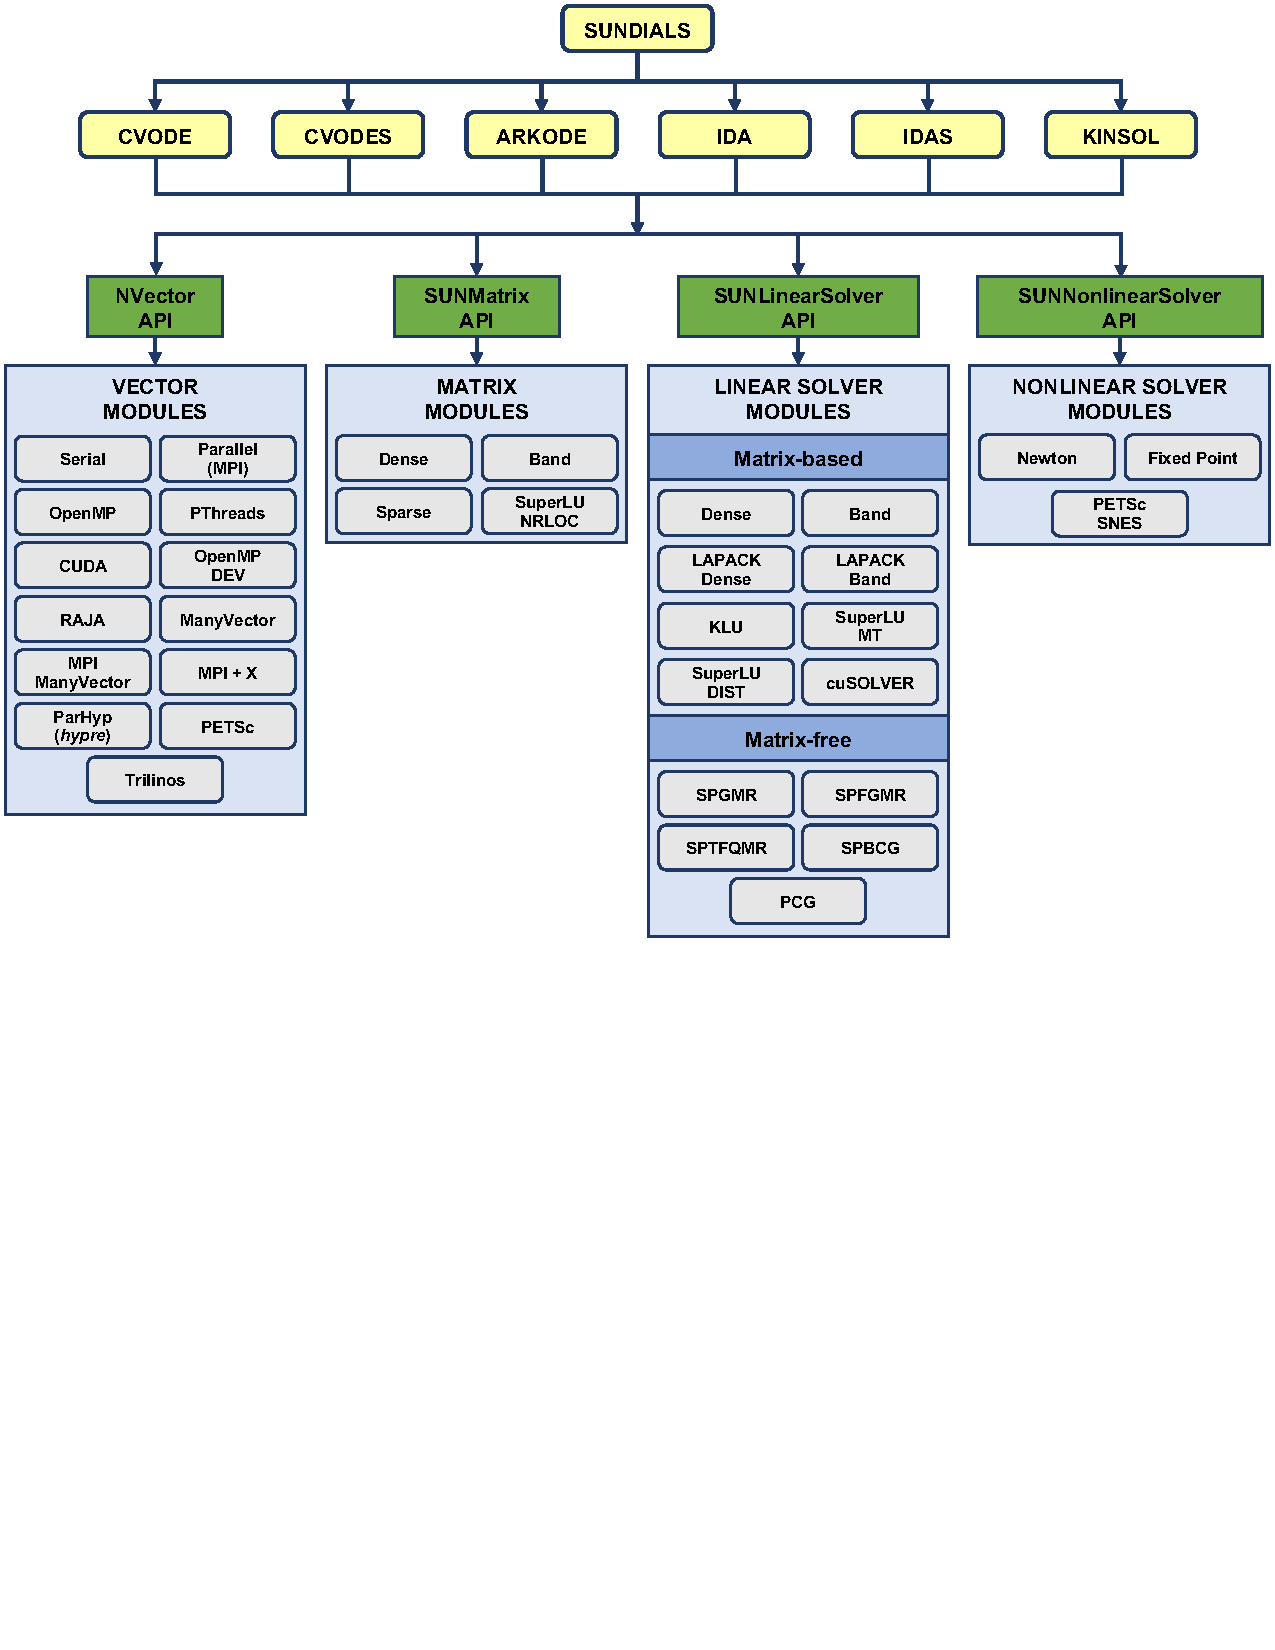
\includegraphics[width=\textwidth]{sunorg1}}}
\caption {High-level diagram of the {\sundials} suite.}\label{f:sunorg1}
\end{figure}
%%
%%
\begin{figure}[htb]
{\centerline{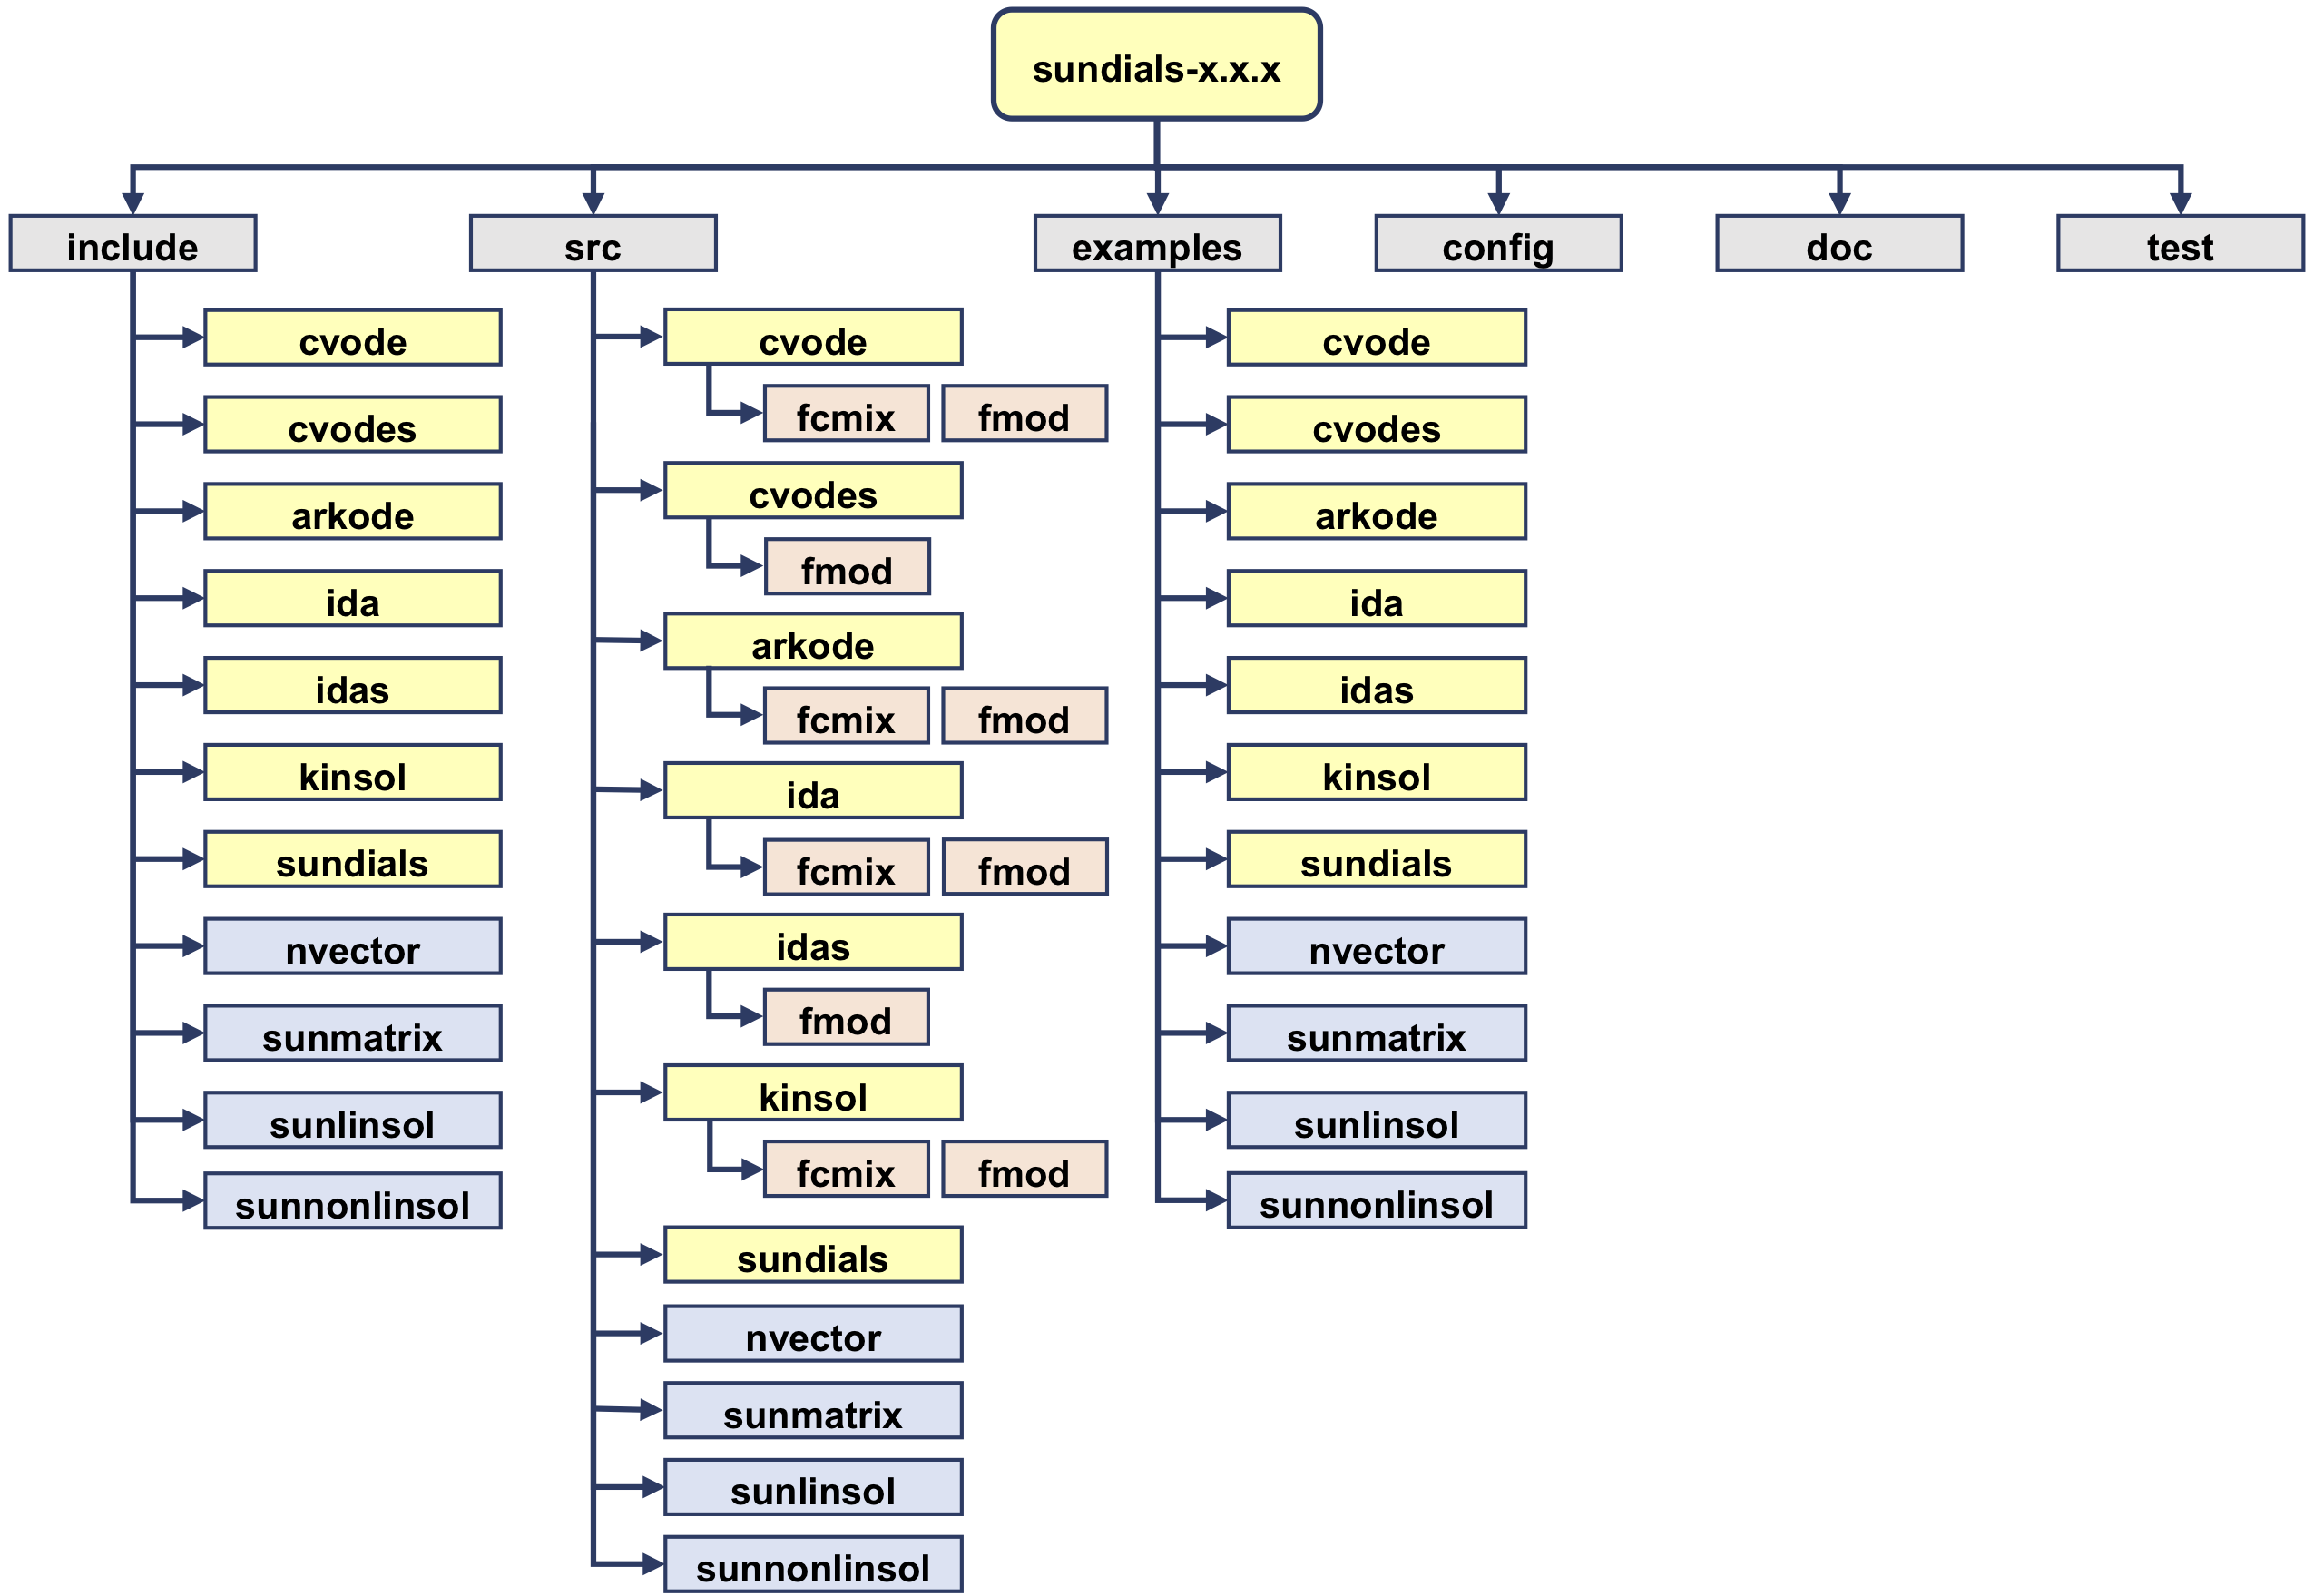
\includegraphics[width=\textwidth]{sunorg2}}}
\caption {Directory structure of the {\sundials} source tree.}\label{f:sunorg2}
\end{figure}
%%
%%
The following is a list of the solver packages presently available, and
the basic functionality of each:
\begin{itemize}

\item {\cvode},
  a solver for stiff and nonstiff ODE systems $dy/dt = f(t,y)$ based
  on Adams and BDF methods;

\item {\cvodes},
  a solver for stiff and nonstiff ODE systems with sensitivity analysis capabilities;

\item {\arkode},
  a solver for stiff, nonstiff, mixed stiff-nonstiff, and multirate ODE systems
  $M dy/dt = f_1(t,y) + f_2(t,y)$ based on Runge-Kutta methods;

\item {\ida},
  a solver for differential-algebraic systems $F(t,y,\dot{y}) = 0$ based on BDF methods;

\item {\idas},
  a solver for differential-algebraic systems
  with sensitivity analysis capabilities;

\item {\kinsol},
  a solver for nonlinear algebraic systems $F(u) = 0$.

\end{itemize}
Note for modules that provide interfaces to third-party libraries (i.e., LAPACK,
{\klu}, {\superlumt}, {\superludist}, {\hypre}, {\petsc}, {\trilinos}, and
{\raja}) users will need to download and compile those packages independently.


%----------------------------------
\section{KINSOL organization}\label{ss:kinsol_org}
%----------------------------------

\index{KINSOL@{\kinsol}!package structure}
The {\kinsol} package is written in the ANSI {\CC} language. This section
summarizes the basic structure of the package, although knowledge
of this structure is not necessary for its use.

The overall organization of the {\kinsol} package is shown in Figure
\ref{f:kinorg}.
\begin{figure}[!htb]
{\centerline{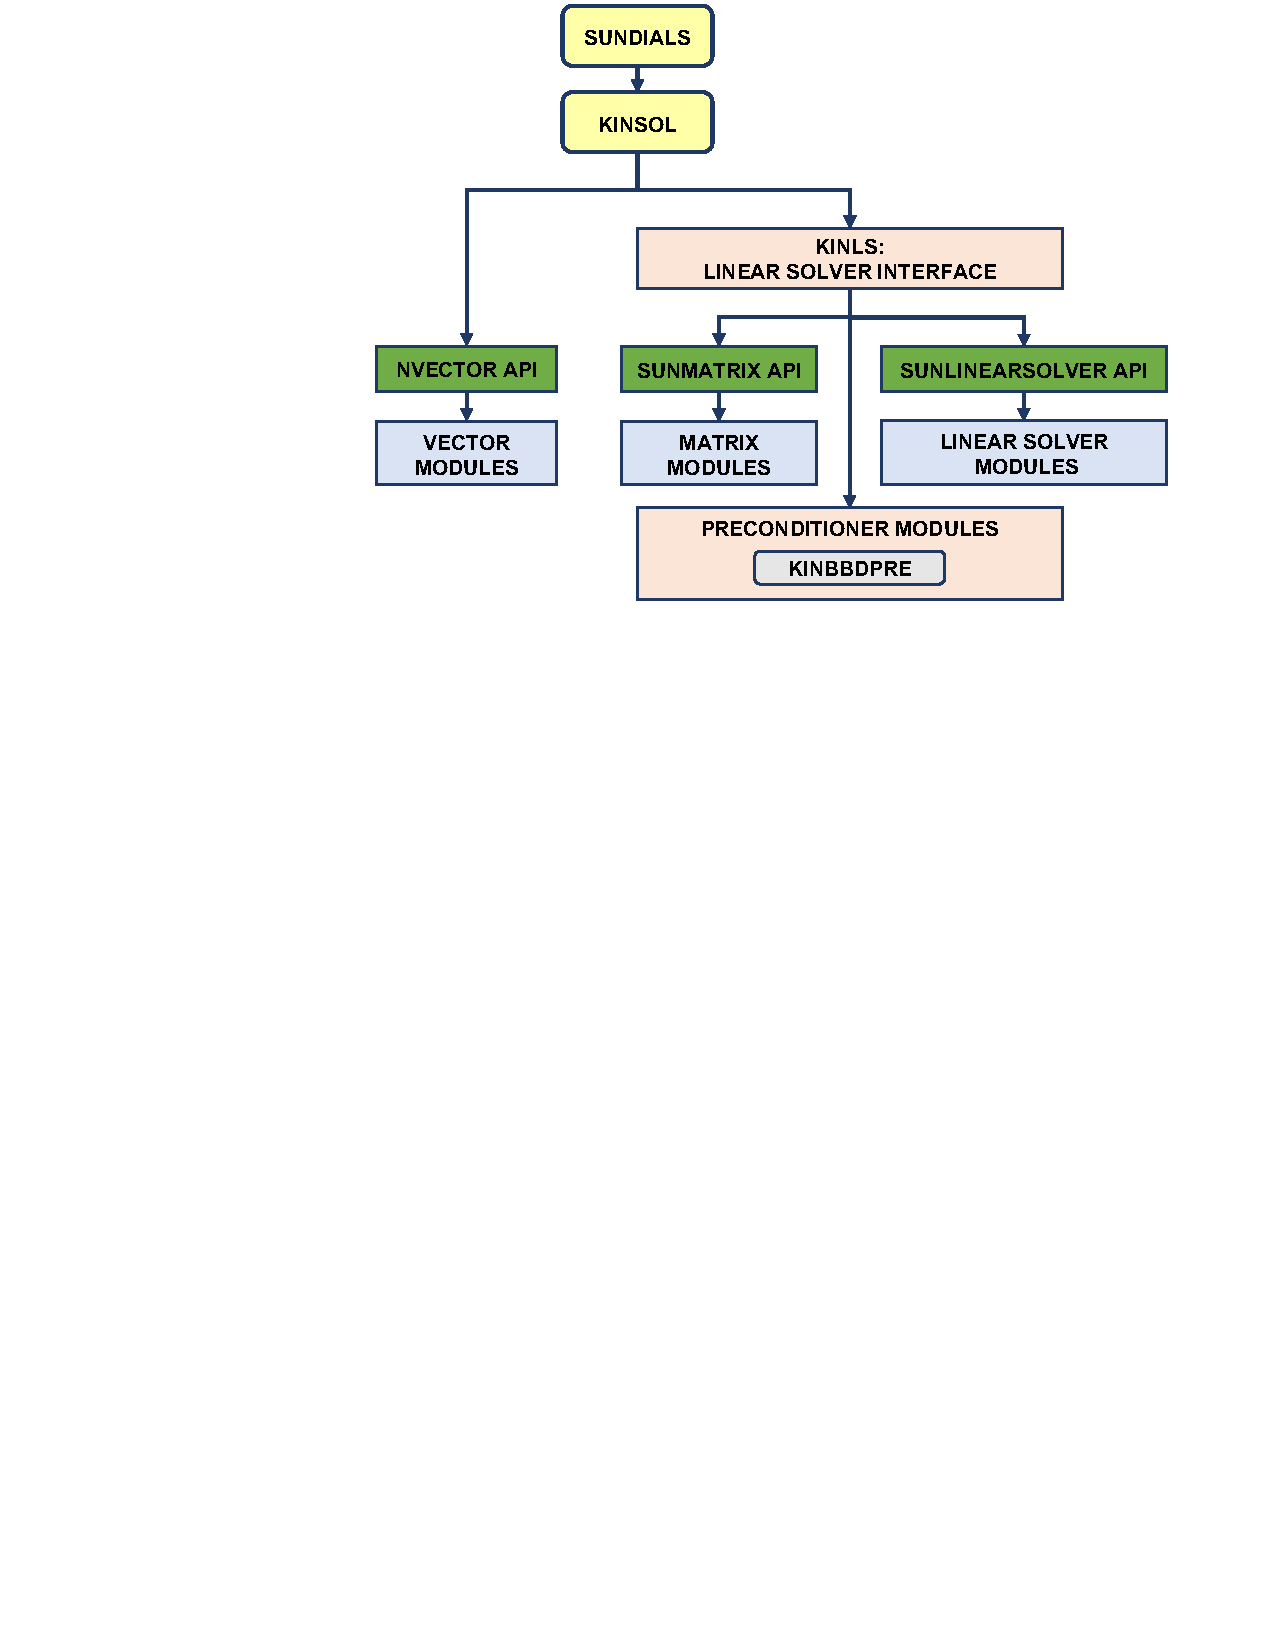
\includegraphics[width=\textwidth]{kinorg}}}
\caption [Overall structure diagram of the KINSOL package]
{Overall structure diagram of the {\kinsol} package.
  Modules specific to {\kinsol} begin with ``KIN'' ({\kinls} and {\kinbbdpre}),
  all other items correspond to generic {\sundials} vector, matrix, and solver
  modules (see Figure \ref{f:sunorg1}).}
\label{f:kinorg}
\end{figure}
The central solver module, implemented in the files
\id{kinsol.h}, \id{kinsol\_impl.h} and \id{kinsol.c}, deals with the solution
of a nonlinear algebraic system using either an Inexact Newton method or a
line search method for the global strategy. Although this module contains logic
for the Newton iteration, it has no knowledge of the method used to solve the
linear systems that arise. For any given user problem, one of the linear system
solver modules is specified, and is then invoked as needed.

\index{KINSOL@{\kinsol} linear solver interfaces|(}
{\kinsol} now has a single unified linear solver interface, {\kinls},
supporting both direct and iterative linear solvers built using the
generic {\sunlinsol} API (see Chapter \ref{s:sunlinsol}).  These
solvers may utilize a {\sunmatrix} object (see Chapter
\ref{s:sunmatrix}) for storing Jacobian information, or they may be
matrix-free. Since {\kinsol} can operate on any valid {\sunlinsol}
implementation, the set of linear solver modules available to
{\kinsol} will expand as new {\sunlinsol} modules are developed.

For users employing dense or banded Jacobian matrices, {\kinls}
includes algorithms for their approximation through difference
quotients, but the user also has the option of supplying the Jacobian
(or an approximation to it) directly.  This user-supplied
routine is required when using sparse or user-supplied Jacobian
matrices.

For users employing matrix-free iterative linear solvers, {\kinls}
includes an algorithm for the approximation by difference quotients of
the product between the Jacobian matrix and a vector, $Jv$. Again, the
user has the option of providing routines for this operation, in two
phases: setup (preprocessing of Jacobian data) and multiplication.

For preconditioned iterative methods, \index{preconditioning!setup and solve phases}
the preconditioning must be supplied by the user, again in two phases:
setup and solve.  While\index{preconditioning!advice on} there is no
default choice of preconditioner analogous to the difference-quotient
approximation in the direct case, the references
\cite{BrHi:89,Byr:92}, together with the example and demonstration
programs included with {\kinsol}, offer considerable assistance in
building preconditioners.

\index{KINSOL@{\kinsol} linear solvers!implementation details|(}
{\kinsol}'s linear solver interface consists of four primary phases,
devoted to (1) memory allocation and initialization, (2) setup of the
matrix data involved, (3) solution of the system, and (4) freeing of memory.
The setup and solution phases are separate because the evaluation of
Jacobians and preconditioners is done only periodically during the
solution, as required to achieve convergence. The call list within
the central {\kinsol} module to each of the associated functions is
fixed, thus allowing the central module to be completely independent
of the linear system method.
\index{KINSOL@{\kinsol} linear solvers!implementation details|)}

{\kinsol} also provides a preconditioner module called {\kinbbdpre} for use
with any of the Krylov iterative linear solvers. It works in conjunction
with {\nvecp} and generates a preconditioner that is
a block-diagonal matrix with each block being a banded matrix, as
further described in \S\ref{sss:kinbbdpre}.

All state information used by {\kinsol} to solve a given problem is saved
in a structure, and a pointer to that structure is returned to the
user.  There is no global data in the {\kinsol} package, and so, in this
respect, it is reentrant. State information specific to the linear
solver is saved in a separate structure, a pointer to which resides in
the {\kinsol} memory structure. The reentrancy of {\kinsol} was motivated
by the anticipated multicomputer extension, but is also essential
in a uniprocessor setting where two or more problems are solved by
intermixed calls to the package from within a single user program.

\clearemptydoublepage
%===============================================================
% Using KINSOL for C applications
%===================================================================================
\chapter{Using KINSOL for C Applications}\label{c:usage}
%===================================================================================

This chapter is concerned with the use of {\kinsol} for the solution
of nonlinear systems. The following subsections treat the header
files, the layout of the user's main program, description of the
{\kinsol} user-callable routines, and user-supplied functions.
The sample programs described in the companion document
\cite{kinsol_ex} may also be helpful.  Those codes may be used as
templates (with the removal of some lines involved in testing), and
are included in the {\kinsol} package.

Users with applications written in {\F} should see Chapter \ref{s:fcmix},
which describes the {\F}/{\CC} interface module.

The user should be aware that not all {\sunlinsol} and {\sunmatrix}
modules are compatible with all {\nvector} implementations.
\index{KINSOL@{\kinsol} linear solvers!NVECTOR@{\nvector} compatibility}
Details on compatability are given in the documentation for each
{\sunmatrix} module (Chapter \ref{s:sunmatrix}) and each {\sunlinsol}
module (Chapter \ref{s:sunlinsol}). For example, {\nvecp} is not
compatible with the dense, banded, or sparse {\sunmatrix} types, or with
the corresponding dense, banded, or sparse {\sunlinsol} modules.  Please
check Chapters \ref{s:sunmatrix} and \ref{s:sunlinsol} to verify
compatability between these modules.  In addition to that
documentation, we note that the preconditioner module {\kinbbdpre}
can only be used with {\nvecp}.
It is not recommended to use a threaded vector module with SuperLU\_MT
unless it is the {\nvecopenmp} module, and SuperLU\_MT is also compiled
with OpenMP.

{\kinsol} uses various constants for both input and output. These are
defined as needed in this chapter, but for convenience are also listed
separately in Appendix \ref{c:constants}.

%%==============================================================================
\section{Access to library and header files}\label{ss:file_access}
%%==============================================================================

At this point, it is assumed that the installation of {\kinsol},
following the procedure described in Appendix \ref{c:install}, has
been completed successfully.

Regardless of where the user's application program resides, its
associated compilation and load commands must make reference to the
appropriate locations for the library and header files required by
{\kinsol}.  The relevant library files are
\begin{itemize}
\item {\em libdir}\id{/libsundials\_kinsol.}{\em lib},
\item {\em libdir}\id{/libsundials\_nvec*.}{\em lib} (one to four files),
\end{itemize}
where the file extension .{\em lib} is typically \id{.so} for shared libraries
and \id{.a} for static libraries. The relevant header files are located in
the subdirectories
\begin{itemize}
\item {\em incdir}\id{/include/kinsol}
\item {\em incdir}\id{/include/sundials}
\item {\em incdir}\id{/include/nvector}
\item {\em incdir}\id{/include/sunmatrix}
\item {\em incdir}\id{/include/sunlinsol}
\end{itemize}
The directories {\em libdir} and {\em incdir} are the install library
and include directories, respectively.  For a default installation,
these are {\em builddir}\id{/lib} and {\em builddir}\id{/include},
respectively, where {\em builddir} was defined in Appendix \ref{c:install}.

%%----------------------------------
\section{Data types}\label{s:types}
%%----------------------------------
% This is a shared SUNDIALS TEX file with description of
% types used in llntyps.h
%
\index{portability}
The \ID{sundials\_types.h} file contains the definition of the type \ID{realtype},
which is used by the {\sundials} solvers for all floating-point data, the definition
of the integer type \ID{sunindextype}, which is used for vector and matrix indices,
and \ID{booleantype}, which is used for certain logic operations within {\sundials}.


\subsection{Floating point types}

The type \id{realtype} can be \id{float}, \id{double}, or \id{long double}, with
the default being \id{double}.
The user can change the precision of the {\sundials} solvers arithmetic at the
configuration stage (see \S\ref{ss:configuration_options_nix}).

Additionally, based on the current precision, \id{sundials\_types.h} defines
\Id{BIG\_REAL} to be the largest value representable as a \id{realtype},
\Id{SMALL\_REAL} to be the smallest value representable as a \id{realtype}, and
\Id{UNIT\_ROUNDOFF} to be the difference between $1.0$ and the minimum \id{realtype}
greater than $1.0$.

Within {\sundials}, real constants are set by way of a macro called
\Id{RCONST}.  It is this macro that needs the ability to branch on the
definition \id{realtype}.  In ANSI {\CC}, a floating-point constant with no
suffix is stored as a \id{double}.  Placing the suffix ``F'' at the
end of a floating point constant makes it a \id{float}, whereas using the suffix
``L'' makes it a \id{long double}.  For example,
\begin{verbatim}
#define A 1.0
#define B 1.0F
#define C 1.0L
\end{verbatim}
defines \id{A} to be a \id{double} constant equal to $1.0$, \id{B} to be a
\id{float} constant equal to $1.0$, and \id{C} to be a \id{long double} constant
equal to $1.0$.  The macro call \id{RCONST(1.0)} automatically expands to \id{1.0}
if \id{realtype} is \id{double}, to \id{1.0F} if \id{realtype} is \id{float},
or to \id{1.0L} if \id{realtype} is \id{long double}.  {\sundials} uses the
\id{RCONST} macro internally to declare all of its floating-point constants.

Additionally, {\sundials} defines several macros for common mathematical
functions \textit{e.g.}, \id{fabs}, \id{sqrt}, \id{exp}, etc. in
\id{sundials\_math.h}. The macros are prefixed with \id{SUNR} and expand to the
appropriate \id{C} function based on the \id{realtype}. For example, the macro
\id{SUNRabs} expands to the \id{C} function \id{fabs} when \id{realtype} is
\id{double}, \id{fabsf} when \id{realtype} is \id{float}, and \id{fabsl} when
\id{realtype} is \id{long double}.

A user program which uses the type \id{realtype}, the \id{RCONST} macro, and the
\id{SUNR} mathematical function macros is precision-independent except for any
calls to  precision-specific library functions. Our example programs use
\id{realtype}, \id{RCONST}, and the \id{SUNR} macros. Users can, however, use
the type \id{double}, \id{float}, or \id{long double} in their code (assuming
that this usage is consistent with the typedef for \id{realtype}) and call the
appropriate math library functions directly. Thus, a previously existing piece
of ANSI {\CC} code can use {\sundials} without modifying the code to use
\id{realtype}, \id{RCONST}, or the \id{SUNR} macros so long as the {\sundials}
libraries use the correct precision (for details see
\S\ref{ss:configuration_options_nix}).


\subsection{Integer types used for indexing}

The type \id{sunindextype} is used for indexing array entries in {\sundials}
modules (\textit{e.g.}, vectors lengths and matrix sizes) as well as for storing
the total problem size. During configuration \id{sunindextype} may be selected
to be either a 32- or 64-bit \emph{signed} integer with the default being
64-bit. See \S\ref{ss:configuration_options_nix} for the configuration option
to select the desired size of \id{sunindextype}. When using a 32-bit integer the
total problem size is limited to $2^{31}-1$ and with 64-bit integers the limit
is $2^{63}-1$. For users with problem sizes that exceed the 64-bit limit an
advanced configuration option is available to specify the type used for
\id{sunindextype}.

A user program which uses \id{sunindextype} to handle indices will work with
both index storage types except for any calls to index storage-specific
external libraries. Our \id{C} and \id{C++} example programs
use \id{sunindextype}. Users can, however, use any compatible type
(\textit{e.g.}, \id{int}, \id{long int}, \id{int32\_t}, \id{int64\_t}, or
\id{long long int}) in their code, assuming that this usage is consistent with
the typedef for \id{sunindextype} on their architecture. Thus, a previously
existing piece of ANSI {\CC} code can use {\sundials} without modifying the code
to use \id{sunindextype}, so long as the {\sundials} libraries use the
appropriate index storage type (for details see
\S\ref{ss:configuration_options_nix}).


%------------------------
\section{Header files}\label{s:header_sol}
%------------------------
\index{header files}
The calling program must include several header files so that various macros
and data types can be used. The header file that is always required is:
%
\begin{itemize}
\item  \Id{kinsol/kinsol.h},
  the header file for {\kinsol}, which defines several
  types and various constants, and includes function prototypes.  This
  includes the header file for {\kinls}, \Id{kinsol/kinsol\_ls.h}.
\end{itemize}
%
\id{kinsol.h} also includes \Id{sundials\_types.h},
which defines the types \id{realtype}, \id{sunindextype}, and \id{booleantype}
and constants \id{SUNFALSE} and \id{SUNTRUE}.

The calling program must also include an {\nvector} implementation header file,
of the form \id{nvector/nvector\_***.h}.  See Chapter \ref{s:nvector} for the appropriate
name.  This file in turn includes the header file \Id{sundials\_nvector.h}
which defines the abstract \Id{N\_Vector} data type.

If using a Newton or Picard nonlinear solver that requires the
solution of a linear system, then a linear solver module header file
will be required.
\index{KINSOL@{\kinsol} linear solvers!header files}
The header files corresponding to the various {\sundials}-provided
linear solver modules available for use with {\kinsol} are:
%%
\begin{itemize}
\item Direct linear solvers:
  \begin{itemize}
  \item \Id{sunlinsol/sunlinsol\_dense.h},
    which is used with the dense linear solver module,
    {\sunlinsoldense};

  \item \Id{sunlinsol/sunlinsol\_band.h},
    which is used with the banded linear solver module,
    {\sunlinsolband};

  \item \Id{sunlinsol/sunlinsol\_lapackdense.h},
    which is used with the LAPACK package dense linear solver module,
    {\sunlinsollapdense};

  \item \Id{sunlinsol/sunlinsol\_lapackband.h},
    which is used with the LAPACK package banded linear solver module,
    {\sunlinsollapband};

  \item \Id{sunlinsol/sunlinsol\_klu.h},
    which is used with the {\klu} sparse linear solver module,
    {\sunlinsolklu};

  \item \Id{sunlinsol/sunlinsol\_superlumt.h},
    which is used with the {\superlumt} sparse linear solver
    module, {\sunlinsolslumt};
  \end{itemize}

\item Iterative linear solvers:
  \begin{itemize}
  \item \Id{sunlinsol/sunlinsol\_spgmr.h},
   which is used with the scaled, preconditioned GMRES Krylov linear
    solver module, {\sunlinsolspgmr};

  \item \Id{sunlinsol/sunlinsol\_spfgmr.h},
    which is used with the scaled, preconditioned FGMRES Krylov linear
    solver module, {\sunlinsolspfgmr};

  \item \Id{sunlinsol/sunlinsol\_spbcgs.h},
    which is used with the scaled, preconditioned Bi-CGStab Krylov
    linear solver module, {\sunlinsolspbcgs};

  \item \Id{sunlinsol/sunlinsol\_sptfqmr.h},
    which is used with the scaled, preconditioned TFQMR Krylov linear
    solver module, {\sunlinsolsptfqmr};

  \item \Id{sunlinsol/sunlinsol\_pcg.h},
    which is used with the scaled, preconditioned CG Krylov linear
    solver module, {\sunlinsolpcg};
  \end{itemize}
\end{itemize}

The header files for the {\sunlinsoldense} and {\sunlinsollapdense}
linear solver modules include the file
\id{sunmatrix/sunmatrix\_dense.h}, which defines the {\sunmatdense}
matrix module, as as well as various functions and macros acting on
such matrices.

The header files for the {\sunlinsolband} and {\sunlinsollapband}
linear solver modules include the file
\id{sunmatrix/sunmatrix\_band.h}, which defines the {\sunmatband}
matrix module, as as well as various functions and macros acting on
such matrices.

The header files for the {\sunlinsolklu} and {\sunlinsolslumt}
sparse linear solvers include the file
\id{sunmatrix/sunmatrix\_sparse.h}, which defines the {\sunmatsparse}
matrix module, as well as various functions and macros acting on such
matrices.

The header files for the Krylov iterative solvers include the file
\id{sundials/sundials\_iterative.h}, which enumerates the kind of
preconditioning, and (for the {\spgmr} and {\spfgmr} solvers) the
choices for the Gram-Schmidt process.

Other headers may be needed, according to the choice of
preconditioner, etc.  For example, in the \id{kinFoodWeb\_kry\_p}
example (see \cite{kinsol_ex}), preconditioning is done with a
block-diagonal matrix. For this, even though the {\sunlinsolspgmr} linear
solver is used, the header \id{sundials/sundials\_dense.h} is included for
access to the underlying generic dense matrix arithmetic routines.

%--------------------------------------------------------------------
\section{A skeleton of the user's main program}\label{ss:skeleton_sol}
%--------------------------------------------------------------------

The following is a skeleton of the user's main program (or calling
program) for the solution of a nonlinear system problem.
Most of the steps are independent of the {\nvector}, {\sunmatrix}, and {\sunlinsol}
implementations used.
For the steps that are not, refer to Chapter \ref{s:nvector},
\ref{s:sunmatrix}, and \ref{s:sunlinsol}  for the
specific name of the function to be called or macro to be referenced.
%%
\index{User main program!KINSOL@{\kinsol} usage}
\begin{Steps}

\item
  {\bf Initialize parallel or multi-threaded environment, if appropriate}

  For example, call \id{MPI\_Init} to initialize {\mpi} if used, or
  set \id{num\_threads}, the number of threads to use within the threaded
  vector functions, if used.

\item
  {\bf Set problem dimensions etc.}

  This generally includes the problem size \id{N}, and may include
  the local vector length \id{Nlocal}.

  Note: The variables \id{N} and \id{Nlocal} should be of type \id{sunindextype}.

\item
  {\bf Set vector with initial guess}

  To set the vector \id{u} of initial guess values, use the appropriate
  functions defined by the particular {\nvector} implementation.

  For native {\sundials} vector implementations
  (except the {\cuda} and {\raja}-based ones), use a call
  of the form \id{u = N\_VMake\_***(..., udata)} if the \id{realtype} array
  \id{udata} containing the initial values of $u$ already exists.
  Otherwise, create a new vector by making a call of the form
  \id{u = N\_VNew\_***(...)}, and then set its elements by accessing
  the underlying data with a call of the form
  \id{ ydata = N\_VGetArrayPointer(u)}.
  See \S\ref{ss:nvec_ser}-\ref{ss:nvec_pthreads} for details.

  For the {\hypre} and {\petsc} vector wrappers, first create and initialize
  the underlying vector and then create an {\nvector} wrapper with a call
  of the form \id{u = N\_VMake\_***(uvec)}, where \id{uvec} is a {\hypre}
  or {\petsc} vector. Note that calls like \id{N\_VNew\_***(...)} and
  \id{N\_VGetArrayPointer(...)} are not available for these vector wrappers.
  See \S\ref{ss:nvec_parhyp} and \S\ref{ss:nvec_petsc} for details.

  If using either the {\cuda}- or {\raja}-based vector implementations
  use a call of the form
  \id{u = N\_VMake\_***(..., c)} where \id{c} is a pointer to a \id{suncudavec}
  or \id{sunrajavec} vector class if this class already exists.  Otherwise,
  create a new vector
  by making a call of the form \id{u = N\_VNew\_***(...)}, and then set its
  elements by accessing the underlying data where it is located
  with a call of the form
  \id{N\_VGetDeviceArrayPointer\_***} or \id{N\_VGetHostArrayPointer\_***}.
  Note that the vector class will allocate memory on both the host and device
  when instantiated.  See \S\ref{ss:nvec_cuda}-\ref{ss:nvec_raja} for details.

%   If a \id{realtype} array \id{udata} containing the initial values of $u$
%   already exists, it may be possible to do this either with a call of the form
%   \id{u = N\_VMake\_***(..., udata);}
%   or by making a call of the form
%   \id{u = N\_VNew\_***(...);}
%   and loading values into the structure defined by \id{NV\_DATA\_***(u)},
%   provided these functions and macro exist for the {\nvector} module chosen.

\item\label{i:kinsol_create}
  {\bf Create {\kinsol} object}

  Call \id{kin\_mem = KINCreate()} to create the {\kinsol} memory block.
  \id{KINCreate} returns a pointer to the {\kinsol} memory structure.
  See \S\ref{sss:kinmalloc} for details.

\item\label{i:kinsol_malloc}
  {\bf Allocate internal memory}

  Call \id{KINInit(...)}
  to specify the problem defining function $F$,
  allocate internal memory for {\kinsol},
  and initialize {\kinsol}.
  \id{KINInit} returns a flag to indicate success or an illegal argument value.
  See \S\ref{sss:kinmalloc} for details.

\item\label{i:matrix}
  {\bf Create matrix object}

  If a matrix-based linear solver is to be used within a Newton or Picard iteration,
  then a template Jacobian matrix must be created by using the
  appropriate functions defined by the particular {\sunmatrix}
  implementation.

  For the {\sundials}-supplied {\sunmatrix} implementations, the
  matrix object may be created using a call of the form

  \id{SUNMatrix J = }\Id{SUNBandMatrix}\id{(...);}

   or

  \id{SUNMatrix J = }\Id{SUNDenseMatrix}\id{(...);}

   or

  \id{SUNMatrix J = }\Id{SUNSparseMatrix}\id{(...);}

  NOTE: The dense, banded, and sparse matrix objects are usable only in a
  serial or threaded environment.

\item\label{i:lin_solver}
  {\bf Create linear solver object}

  If a Newton or Picard iteration is chosen, then the desired linear solver
  object must be created by using the appropriate functions defined by
  the particular {\sunlinsol} implementation.

  For any of the {\sundials}-supplied {\sunlinsol} implementations,
  the linear solver object may be created using a call of the form

  \id{SUNLinearSolver LS = SUNLinSol\_*(...);}

  where \id{*} can be replaced with ``Dense'', ``SPGMR'', or other
  options, as discussed in \S\ref{sss:lin_solv_init} and Chapter {\ref{s:sunlinsol}}.

\item
  {\bf Set linear solver optional inputs}

  Call \id{*Set*} functions from the selected linear solver module
  to change optional inputs specific to that linear solver.
  See the documentation for each {\sunlinsol} module in Chapter
  {\ref{s:sunlinsol}} for details.

\item\label{i:lin_solver_interface}
  {\bf Attach linear solver module}

  If a Newton or Picard iteration is chosen, initialize the {\kinls}
  linear solver interface by attaching the linear solver object (and
  matrix object, if applicable) with one of the following calls (for
  details see \S\ref{sss:lin_solv_init}):

  \id{ier = }\Id{KINSetLinearSolver}\id{(...);}

\item
  {\bf Set optional inputs}

  Call \id{KINSet*} routines to change from their default values any
  optional inputs that control the behavior of {\kinsol}.
  See \S\ref{ss:optional_input} for details.

\item
  {\bf Solve problem}

  Call \id{ier = }\Id{KINSol}\id{(...)} to solve the nonlinear problem for a given
  initial guess. See \S\ref{sss:kinsol} for details.

\item
  {\bf Get optional outputs}

  Call \id{KINGet*} functions to obtain optional output.
  See \S\ref{ss:optional_output} for details.

\item
  {\bf Deallocate memory for solution vector}

  Upon completion of the solution, deallocate memory for the vector \id{u} by
  calling the appropriate destructor function defined by the {\nvector} implementation:

  \id{N\_VDestroy(u);}

\item
  {\bf Free solver memory}

  Call \id{KINFree(\&kin\_mem)} to free the memory allocated for {\kinsol}.

\item
  {\bf Free linear solver and matrix memory}

  Call \Id{SUNLinSolFree} and \ID{SUNMatDestroy} to free any memory
  allocated for the linear solver and matrix objects created above.

\item
  {\bf Finalize MPI, if used}

  Call \id{MPI\_Finalize()} to terminate {\mpi}.

\end{Steps}

\input{linear-vector-table}

%%==============================================================================

\section{User-callable functions}\label{s:kinsol_fct_sol}

This section describes the {\kinsol} functions that are called by the
user to set up and solve a nonlinear problem. Some of these are required.
However, starting with \S\ref{ss:optional_input}, the functions listed involve
optional inputs/outputs or restarting, and those paragraphs can be
skipped for a casual use of {\kinsol}. In any case, refer to
\S\ref{ss:skeleton_sol} for the correct order of these calls.

The return flag (when present) for each of these routines is a
negative integer if an error occurred, and non-negative otherwise.

%%-------------------------------------------------------------------------------

\subsection{KINSOL initialization and deallocation functions}
\label{sss:kinmalloc}

The following three functions must be called in the order listed. The last one
is to be called only after the problem solution is complete, as it frees the
{\kinsol} memory block created and allocated by the first two calls.
%%
\ucfunction{KINCreate}
{
  kin\_mem = KINCreate();
}
{
  The function \ID{KINCreate} instantiates a {\kinsol} solver object.
}
{
  This function has no arguments.
}
{
  If successful, \id{KINCreate} returns a pointer to the newly created
  {\kinsol} memory block (of type \id{void *}).
  If an error occurred, \id{KINCreate} prints an error message to \id{stderr}
  and returns \id{NULL}.
}
{}
%%
%%
\ucfunction{KINInit}
{
flag = KINInit(kin\_mem, func, tmpl);
}
{
  The function \ID{KINInit} specifies the problem-defining
  function, allocates internal memory, and initializes {\kinsol}.
}
{
  \begin{args}[kin\_mem]
  \item[kin\_mem] (\id{void *})
    pointer to the {\kinsol} memory block returned by \id{KINCreate}.
  \item[func] (\Id{KINSysFn})
    is the {\CC} function which computes the system function $F$
    (or $G(u)$ for fixed-point iteration) in the nonlinear
    problem.  This function has the form \id{func(u, fval, user\_data)}.
    (For full details see \S\ref{ss:sysFn}.)
  \item[tmpl] (\id{N\_Vector})
    is any \id{N\_Vector} (e.g. the initial guess vector \id{u}) which is used
    as a template to create (by cloning) necessary vectors in \id{kin\_mem}.
  \end{args}
}
{
  The return value \id{flag} (of type \id{int}) will be one of the following:
  \begin{args}[KIN\_ILL\_INPUT]
  \item[\Id{KIN\_SUCCESS}]
    The call to \id{KINInit} was successful.
  \item[\Id{KIN\_MEM\_NULL}]
    The {\kinsol} memory block was not initialized through a previous call
    to \id{KINCreate}.
  \item[\Id{KIN\_MEM\_FAIL}]
    A memory allocation request has failed.
  \item[\Id{KIN\_ILL\_INPUT}]
    An input argument to \id{KINInit} has an illegal value.
  \end{args}
}
{
  If an error occurred, \id{KINInit} sends an error message to the
  error handler function.
}
%%
%%
\ucfunction{KINFree}
{
  KINFree(\&kin\_mem);
}
{
  The function \ID{KINFree} frees the memory allocated by
  a previous call to \id{KINCreate}.
}
{
  The argument is the address of the pointer to the {\kinsol} memory block
  returned by \id{KINCreate} (of type \id{void *}).
}
{
  The function \id{KINFree} has no return value.
}
{}
%%

%%-------------------------------------------------------------------------------

\subsection{Linear solver specification function}\label{sss:lin_solv_init}

As previously explained, Newton and Picard iterations require the solution of
linear systems of the form $J\delta = -F$. Solution of these linear
systems is handled using the {\kinls} linear solver interface.  This
interface supports all valid {\sunlinsol} modules.  Here, matrix-based
{\sunlinsol} modules utilize {\sunmatrix} objects to store the
Jacobian matrix $J = \partial{F}/\partial{u}$ and factorizations used
throughout the solution process.  Conversely, matrix-free {\sunlinsol}
modules instead use iterative methods to solve the linear systems of
equations, and only require the \emph{action} of the Jacobian on a
vector, $Jv$.

With most iterative linear solvers, preconditioning can be done on the
left only, on the right only, on both the left and the right, or not
at all.  However, only right preconditioning is supported within
{\kinls}.  If preconditioning is done, user-supplied
functions define the linear operator corresponding to a right
preconditioner matrix $P$, which should approximate the system
Jacobian matrix $J$.  For the specification of a preconditioner, see
the iterative linear solver sections in \S\ref{ss:optional_input} and
\S\ref{ss:user_fct_sol}. A preconditioner matrix $P$ must approximate
the Jacobian $J$, at least crudely.

\index{KINSOL{\kinsol} linear solvers!selecting one|(}
To specify a generic linear solver to {\kinsol}, after the call to
\id{KINCreate} but before any calls to \id{KINSol}, the user's
program must create the appropriate {\sunlinsol} object and call
the function \Id{KINSetLinearSolver}, as documented below.
To create the \id{SUNLinearSolver} object, the user may call one of
the {\sundials}-packaged {\sunlinsol} module constructor routines via
a call of the form

\begin{verbatim}
      SUNLinearSolver LS = SUNLinSol_*(...);
\end{verbatim}

The current list of such constructor routines includes
\Id{SUNLinSol\_Dense},
\Id{SUNLinSol\_Band},
\Id{SUNLinSol\_LapackDense},
\Id{SUNLinSol\_LapackBand},
\Id{SUNLinSol\_KLU},
\Id{SUNLinSol\_SuperLUMT},
\Id{SUNLinSol\_SPGMR},
\Id{SUNLinSol\_SPFGMR},
\Id{SUNLinSol\_SPBCGS},
\Id{SUNLinSol\_SPTFQMR}, and
\Id{SUNLinSol\_PCG}.

Alternately, a user-supplied
\id{SUNLinearSolver} module may be created and used instead.  The use
of each of the generic linear solvers involves certain constants,
functions and possibly some macros, that are likely to be needed in
the user code.  These are available in the corresponding header file
associated with the specific {\sunmatrix} or {\sunlinsol} module in
question, as described in Chapters \ref{s:sunmatrix} and
\ref{s:sunlinsol}.

Once this solver object has been constructed, the user should attach
it to {\kinsol} via a call to \Id{KINSetLinearSolver}.  The first
argument passed to this function is the {\kinsol} memory pointer
returned by \id{KINCreate}; the second argument is the desired
{\sunlinsol} object to use for solving Newton or Picard systems.  The
third argument is an optional {\sunmatrix} object to accompany
matrix-based {\sunlinsol} inputs (for matrix-free linear solvers, the
third argument should be \id{NULL}).  A call to this function
initializes the {\kinls} linear solver interface, linking it to the
main {\kinsol} solver, and allows the user to specify additional
parameters and routines pertinent to their choice of linear solver.
%%
\index{KINSOL@{\kinsol} linear solvers!selecting one|)}
\index{KINSOL@{\kinsol} linear solver interface!KINLS@{\kinls}}
\ucfunction{KINSetLinearSolver}
{
  flag = KINSetLinearSolver(kin\_mem, LS, J);
}
{
  The function \ID{KINSetLinearSolver} attaches a generic {\sunlinsol}
  object \id{LS} and corresponding template Jacobian {\sunmatrix}
  object \id{J} (if applicable) to {\kinsol}, initializing the
  {\kinls} linear solver interface.
}
{
  \begin{args}[kin\_mem]
  \item[kin\_mem] (\id{void *})
    pointer to the {\kinsol} memory block.
  \item[LS] (\id{SUNLinearSolver})
    {\sunlinsol} object to use for solving Newton linear systems.
  \item[J] (\id{SUNMatrix})
    {\sunmatrix} object for used as a template for the Jacobian (or
    \id{NULL} if not applicable).
  \end{args}
}
{
  The return value \id{flag} (of type \id{int}) is one of
  \begin{args}
  [KINLS\_ILL\_INPUT]
  \item[\Id{KINLS\_SUCCESS}]
    The {\kinls} initialization was successful.
  \item[\Id{KINLS\_MEM\_NULL}]
    The \id{kin\_mem} pointer is \id{NULL}.
  \item[\Id{KINLS\_ILL\_INPUT}]
    The {\kinls} interface is not compatible with the \id{LS} or
    \id{J} input objects or is incompatible with the current
    {\nvector} module.
  \item[\Id{KINLS\_SUNLS\_FAIL}]
    A call to the \id{LS} object failed.
  \item[\Id{KINLS\_MEM\_FAIL}]
    A memory allocation request failed.
  \end{args}
}
{
  If \id{LS} is a matrix-based linear solver, then the template
  Jacobian matrix \id{J} will be used in the solve process, so if
  additional storage is required within the {\sunmatrix} object
  (e.g. for factorization of a banded matrix), ensure that the input
  object is allocated with sufficient size (see the documentation of
  the particular {\sunmatrix} type in Chapter \ref{s:sunmatrix} for
  further information).

  The previous routines \Id{KINDlsSetLinearSolver} and
  \Id{KINSpilsSetLinearSolver} are now wrappers for this routine, and may
  still be used for backward-compatibility.  However, these will be
  deprecated in future releases, so we recommend that users transition
  to the new routine name soon.
}
%%
%%
%%

%--------------------------------------------------------------------
\subsection{KINSOL solver function}\label{sss:kinsol}
%--------------------------------------------------------------------

This is the central step in the solution process, the call to solve
the nonlinear algebraic system.
%
\ucfunction{KINSol}
{
  flag = KINSol(kin\_mem, u, strategy, u\_scale, f\_scale);
}
{
  The function \ID{KINSol} computes an approximate solution to the nonlinear
  system.
}
{
  \begin{args}[strategy]
  \item[kin\_mem] (\id{void *})
    pointer to the {\kinsol} memory block.
  \item[u] (\id{N\_Vector})
    vector set to initial guess by user before calling \id{KINSol},
    but which upon return contains an approximate solution of
    the nonlinear system $F(u) = 0$.
  \item[strategy] (\id{int})
    strategy used to solve the nonlinear system. It must be of the following: \\
    \ID{KIN\_NONE}  basic Newton iteration \\
    \ID{KIN\_LINESEARCH} Newton with globalization \\
    \ID{KIN\_FP} fixed-point iteration with Anderson Acceleration
                 (no linear solver needed)\\
    \ID{KIN\_PICARD} Picard iteration with Anderson Acceleration
                     (uses a linear solver)\\
  \item[u\_scale] (\id{N\_Vector})
    vector containing diagonal elements of scaling matrix $D_u$ for vector \id{u}
    chosen so that the components of $D_u \cdot$\id{u}
    (as a matrix multiplication) all have roughly the same magnitude when
    \id{u} is close to a root of $F(u)$.
  \item[f\_scale] (\id{N\_Vector})
    vector containing diagonal elements of scaling matrix $D_F$ for $F(u)$ chosen
    so that the components of $D_F \cdot F($\id{u}$)$
    (as a matrix multiplication) all have roughly the same magnitude when
    \id{u} is not too near a root of $F(u)$. In the case of a fixed-point
    iteration, consider $F(u) = G(u) - u$.
  \end{args}
}
{
  On return, \id{KINSol} returns the approximate solution in the vector \id{u}
  if successful.  The return value \id{flag} (of type \id{int}) will be one of
  the following:
  \begin{args}[a]

  \item[\Id{KIN\_SUCCESS}]\rule{0pt}{0pt}

    \id{KINSol} succeeded; the scaled norm of $F(u)$ is less than \id{fnormtol}.

  \item[\Id{KIN\_INITIAL\_GUESS\_OK}]\rule{0pt}{0pt}

    The guess \id{u} $=u_0$ satisfied the system $F(u)=0$
    within the tolerances specified (the scaled norm of $F(u_0)$ is less than
    0.01*\id{fnormtol}).

  \item[\Id{KIN\_STEP\_LT\_STPTOL}]\rule{0pt}{0pt}

    {\kinsol} stopped based on scaled step length.
    This means that the current iterate may be an approximate solution of the given
    nonlinear system, but it is also quite possible that the algorithm is ``stalled"
    (making insufficient progress) near an invalid solution, or that the
    scalar \id{scsteptol} is too large (see \id{KINSetScaledStepTol} in
    \S\ref{ss:optional_input} to change \id{scsteptol} from its default value).

  \item[\Id{KIN\_MEM\_NULL}]\rule{0pt}{0pt}

    The {\kinsol} memory block pointer was \id{NULL}.

  \item[\Id{KIN\_ILL\_INPUT}]\rule{0pt}{0pt}

    An input parameter was invalid.

  \item[\Id{KIN\_NO\_MALLOC}]\rule{0pt}{0pt}

    The {\kinsol} memory was not allocated by a call to \id{KINCreate}.

  \item[\Id{KIN\_MEM\_FAIL}]\rule{0pt}{0pt}

    A memory allocation failed.

  \item[\Id{KIN\_LINESEARCH\_NONCONV}]\rule{0pt}{0pt}

    The line search algorithm was unable to find an iterate sufficiently distinct
    from the current iterate, or could not find an iterate satisfying
    the sufficient decrease condition.

    Failure to satisfy the sufficient decrease condition could mean the current
    iterate is ``close" to an approximate solution of the given nonlinear system,
    the difference approximation of the matrix-vector product $J(u) v$ is inaccurate,
    or the real scalar \id{scsteptol} is too large.

  \item[\Id{KIN\_MAXITER\_REACHED}] \rule{0pt}{0pt}

    The maximum number of nonlinear iterations has been reached.

  \item[\Id{KIN\_MXNEWT\_5X\_EXCEEDED}]\rule{0pt}{0pt}

    Five consecutive steps have been taken that satisfy the inequality
    $\|D_u p\|_{L2} > 0.99 \,$ \id{mxnewtstep}, where $p$ denotes the current step
    and \id{mxnewtstep} is a scalar upper bound on the scaled step length.
    Such a failure may mean that $\|D_F F(u)\|_{L2}$ asymptotes from above to a
    positive value, or the real scalar \id{mxnewtstep} is too small.

  \item[\Id{KIN\_LINESEARCH\_BCFAIL}]\rule{0pt}{0pt}

    The line search algorithm was unable to satisfy the ``beta-condition'' for
    \id{MXNBCF} $+ 1$ nonlinear iterations (not necessarily consecutive),
    which may indicate the algorithm is making poor progress.

  \item[\Id{KIN\_LINSOLV\_NO\_RECOVERY}]\rule{0pt}{0pt}

    The user-supplied routine \id{psolve} encountered a recoverable error, but
    the preconditioner is already current.

  \item[\Id{KIN\_LINIT\_FAIL}]\rule{0pt}{0pt}

    The {\kinls} initialization routine (\id{linit}) encountered an error.

  \item[\Id{KIN\_LSETUP\_FAIL}]\rule{0pt}{0pt}

    The {\kinls} setup routine (\id{lsetup}) encountered an error;
    e.g., the user-supplied routine \id{pset} (used to set up the
    preconditioner data) encountered an unrecoverable error.

  \item[\Id{KIN\_LSOLVE\_FAIL}]\rule{0pt}{0pt}

    The {\kinls} solve routine (\id{lsolve}) encountered an error;
    e.g., the user-supplied routine \id{psolve} (used to to solve the preconditioned
    linear system) encountered an unrecoverable error.

  \item[\Id{KIN\_SYSFUNC\_FAIL}]\rule{0pt}{0pt}

    The system function failed in an unrecoverable manner.

  \item[\Id{KIN\_FIRST\_SYSFUNC\_ERR}]\rule{0pt}{0pt}

    The system function failed recoverably at the first call.

  \item[\Id{KIN\_REPTD\_SYSFUNC\_ERR}]\rule{0pt}{0pt}

    The system function had repeated recoverable errors. No recovery is possible.


  \end{args}
}
{
  The components of vectors \id{u\_scale} and \id{f\_scale} should be strictly positive.

  \id{KIN\_SUCCESS} $=0$, \id{KIN\_INITIAL\_GUESS\_OK} $=1$, and
  \id{KIN\_STEP\_LT\_STPTOL} $=2$.
  %%
  All remaining return values are negative and therefore a test \id{flag} $< 0$
  will trap all \id{KINSol} failures.
}


%%==============================================================================
\subsection{Optional input functions}\label{ss:optional_input}
%%==============================================================================

There are numerous optional input parameters that control the behavior
of the {\kinsol} solver.  {\kinsol} provides functions that can be used
to change these from their default values.  Table \ref{t:optional_input}
lists all optional input functions in {\kinsol} which are then
described in detail in the remainder of this section, beginning with
those for the main {\kinsol} solver and continuing with those for the
{\kinls} linear solver interface. For the most casual use of {\kinsol}, the
reader can skip to \S\ref{ss:user_fct_sol}.

We note that, on error return, all of these functions also send an error message
to the error handler function.\index{error messages}
We also note that all error return values are negative, so a test \id{flag} $<0$
will catch any error.

\begin{table}
\centering
\caption{Optional inputs for {\kinsol} and {\kinls}}
\label{t:optional_input}
\medskip
\begin{tabular}{|l|l|l|}\hline
{\bf Optional input} & {\bf Function name} & {\bf Default} \\
\hline
\multicolumn{3}{|c|}{\bf KINSOL main solver} \\
\hline
Error handler function & \id{KINSetErrHandlerFn} & internal fn. \\
Pointer to an error file & \id{KINSetErrFile} & \id{stderr}  \\
Info handler function & \id{KINSetInfoHandlerFn} & internal fn. \\
Pointer to an info file & \id{KINSetInfoFile} & \id{stdout} \\
Data for problem-defining function & \id{KINSetUserData} & \id{NULL} \\
Verbosity level of output & \id{KINSetPrintLevel} & 0 \\
Max. number of nonlinear iterations & \id{KINSetNumMaxIters} & 200 \\
No initial matrix setup & \id{KINSetNoInitSetup} & \id{SUNFALSE} \\
No residual monitoring${}^{*}$ & \id{KINSetNoResMon} & \id{SUNFALSE} \\
Max. iterations without matrix setup & \id{KINSetMaxSetupCalls} & 10 \\
Max. iterations without residual check${}^{*}$ & \id{KINSetMaxSubSetupCalls} & 5 \\
Form of $\eta$ coefficient & \id{KINSetEtaForm} &  \id{KIN\_ETACHOICE1}\\
Constant value of $\eta$ & \id{KINSetEtaConstValue} &  0.1 \\
Values of $\gamma$ and $\alpha$ & \id{KINSetEtaParams} & 0.9 and 2.0 \\
Values of $\omega_{min}$ and $\omega_{max}$${}^{*}$ & \id{KINSetResMonParams} & 0.00001 and 0.9 \\
Constant value of $\omega$${}^{*}$ & \id{KINSetResMonConstValue} & 0.9 \\
Lower bound on $\epsilon$ & \id{KINSetNoMinEps} & \id{SUNFALSE} \\
Max. scaled length of Newton step & \id{KINSetMaxNewtonStep} & $1000 \| D_u u_0 \|_2$ \\
Max. number of $\beta$-condition failures & \id{KINSetMaxBetaFails} & 10 \\
Rel. error for D.Q. $Jv$ & \id{KINSetRelErrFunc} & $\sqrt{\text{uround}}$ \\
Function-norm stopping tolerance & \id{KINSetFuncNormTol} & uround$^{1/3}$ \\
Scaled-step stopping tolerance & \id{KINSetScaledSteptol} & $\text{uround}^{2/3}$ \\
Inequality constraints on solution & \id{KINSetConstraints} & \id{NULL} \\
Nonlinear system function & \id{KINSetSysFunc} & none \\
Anderson Acceleration subspace size & \id{KINSetMAA} & 0 \\
\hline
\multicolumn{3}{|c|}{\bf KINLS linear solver interface} \\
\hline
Jacobian function & \id{KINSetJacFn} &  DQ \\
Preconditioner functions and data & \id{KINSetPreconditioner} & \id{NULL}, \id{NULL}, \id{NULL} \\
Jacobian-times-vector function and data & \id{KINSetJacTimesVecFn} & internal DQ, \\
&&\id{NULL} \\
\hline
\end{tabular}
\end{table}

\subsubsection{Main solver optional input functions}\label{ss:optin_main}
\index{optional input!solver|(}

The calls listed here can be executed in any order. However, if either of the
functions \id{KINSetErrFile} or \id{KINSetErrHandlerFn} is to be called, that
call should be first, in order to take effect for any later error message.
%%
\index{error messages!redirecting}
\ucfunction{KINSetErrFile}
{
flag = KINSetErrFile(kin\_mem, errfp);
}
{
  The function \ID{KINSetErrFile} specifies the pointer to the file
  where all {\kinsol} messages should be directed when the default
  {\kinsol} error handler function is used.
}
{
  \begin{args}[kin\_mem]
  \item[kin\_mem] (\id{void *})
    pointer to the {\kinsol} memory block.
  \item[errfp] (\id{FILE *})
    pointer to output file.
  \end{args}
}
{
  The return value \id{flag} (of type \id{int}) is one of
  \begin{args}[KIN\_MEM\_NULL]
  \item[\Id{KIN\_SUCCESS}]
    The optional value has been successfully set.
  \item[\Id{KIN\_MEM\_NULL}]
    The \id{kin\_mem} pointer is \id{NULL}.
  \end{args}
}
{
  The default value for \id{errfp} is \id{stderr}.

  Passing a value of \id{NULL} disables all future error message output
  (except for the case in which the {\kinsol} memory pointer is \id{NULL}).
  This use of \id{KINSetErrFile} is strongly discouraged.

  {\warn}If \id{KINSetErrFile} is to be called, it should be called before any
  other optional input functions, in order to take effect for any later error message.
}
%%
\index{error message!user-defined handler}
\ucfunction{KINSetErrHandlerFn}
{
flag = KINSetErrHandlerFn(kin\_mem, ehfun, eh\_data);
}
{
  The function \ID{KINSetErrHandlerFn} specifies the optional user-defined function
  to be used in handling error messages.
}
{
  \begin{args}[kin\_mem]
  \item[kin\_mem] (\id{void *})
    pointer to the {\kinsol} memory block.
  \item[ehfun] (\id{KINErrHandlerFn})
    is the user's {\CC} error handler function (see \S\ref{ss:ehFn}).
  \item[eh\_data] (\id{void *})
    pointer to user data passed to \id{ehfun} every time it is called.
  \end{args}
}
{
  The return value \id{flag} (of type \id{int}) is one of:
  \begin{args}[KIN\_MEM\_NULL]
  \item[\Id{KIN\_SUCCESS}]
    The function \id{ehfun} and data pointer \id{eh\_data} have been successfully set.
  \item[\Id{KIN\_MEM\_NULL}]
    The \id{kin\_mem} pointer is \id{NULL}.
  \end{args}
}
{
  The default internal error handler function directs error messages to the
  file specified by the file pointer \id{errfp} (see \id{KINSetErrFile} above).

  Error messages indicating that the {\kinsol} solver memory is \id{NULL} will
  always be directed to \id{stderr}.
}
%%
\index{info messages!redirecting}
\ucfunction{KINSetInfoFile}
{
flag = KINSetInfoFile(kin\_mem, infofp);
}
{
  The function \ID{KINSetInfoFile} specifies the pointer to the file
  where all informative (non-error) messages should be directed.
}
{
  \begin{args}[kin\_mem]
  \item[kin\_mem] (\id{void *})
    pointer to the {\kinsol} memory block.
  \item[infofp] (\id{FILE *})
    pointer to output file.
  \end{args}
}
{
  The return value \id{flag} (of type \id{int}) is one of:
  \begin{args}[KIN\_MEM\_NULL]
  \item[\Id{KIN\_SUCCESS}]
    The optional value has been successfully set.
  \item[\Id{KIN\_MEM\_NULL}]
    The \id{kin\_mem} pointer is \id{NULL}.
  \end{args}
}
{
  The default value for \id{infofp} is \id{stdout}.
}
%%
%%
\index{info message!user-defined handler}
\ucfunction{KINSetInfoHandlerFn}
{
flag = KINSetInfoHandlerFn(kin\_mem, ihfun, ih\_data);
}
{
  The function \ID{KINSetInfoHandlerFn} specifies the optional user-defined function
  to be used in handling informative (non-error) messages.
}
{
  \begin{args}[kin\_mem]
  \item[kin\_mem] (\id{void *})
    pointer to the {\kinsol} memory block.
  \item[ihfun] (\id{KINInfoHandlerFn})
    is the user's {\CC} information handler function (see \S\ref{ss:ihFn}).
  \item[ih\_data] (\id{void *})
    pointer to user data passed to \id{ihfun} every time it is called.
  \end{args}
}
{
  The return value \id{flag} (of type \id{int}) is one of:
  \begin{args}[KIN\_MEM\_NULL]
  \item[\Id{KIN\_SUCCESS}]
    The function \id{ihfun} and data pointer \id{ih\_data} have been successfully set.
  \item[\Id{KIN\_MEM\_NULL}]
    The \id{kin\_mem} pointer is \id{NULL}.
  \end{args}
}
{
  The default internal information handler function directs informative (non-error)
  messages to the file specified by the file pointer \id{infofp} (see
  \id{KINSetInfoFile} above).
}
%%
%%
\ucfunction{KINSetPrintLevel}
{
flag = KINSetPrintLevel(kin\_mem, printfl);
}
{
  The function \ID{KINSetPrintLevel} specifies the level of verbosity
  of the output.
}
{
  \begin{args}[kin\_mem]

  \item[kin\_mem] (\id{void *})
    pointer to the {\kinsol} memory block.

  \item[printfl] (\id{int})
    flag indicating the level of verbosity. Must be one of:

    \begin{itemize}
    \item[0]
      no information displayed.

    \item[1]
      for each nonlinear iteration display
      the following information: the scaled
      Euclidean $\ell_2$ norm of the system function
      evaluated at the current iterate, the
      scaled norm of the Newton step (only if
      using \id{KIN\_NONE}), and the
      number of function evaluations performed
      so far.

    \item[2]
      display level 1 output and the
      following values for each iteration:

      $\|F(u)\|_{D_F}$
      (only for \id{KIN\_NONE}).

      $\|F(u)\|_{D_F,\infty}$
      (for \id{KIN\_NONE} and
      \id{KIN\_LINESEARCH}).

    \item[3]
      display level 2 output plus additional
      values used by the global strategy
      (only if using \id{KIN\_LINESEARCH}), and
      statistical information for iterative linear
      solver modules.
    \end{itemize}

  \end{args}
}
{
  The return value \id{flag} (of type \id{int}) is one of:
  \begin{args}[KIN\_ILL\_INPUT]
  \item[\Id{KIN\_SUCCESS}]
    The optional value has been successfully set.
  \item[\Id{KIN\_MEM\_NULL}]
    The \id{kin\_mem} pointer is \id{NULL}.
  \item[\Id{KIN\_ILL\_INPUT}]
    The argument \id{printfl} had an illegal value.
  \end{args}
}
{
  The default value for \id{printfl} is $0$.
}
%%
\ucfunction{KINSetUserData}
{
flag = KINSetUserData(kin\_mem, user\_data);
}
{
  The function \ID{KINSetUserData} specifies the pointer to user-defined memory
  that is to be passed to all user-supplied functions.
}
{
  \begin{args}[kin\_mem]
  \item[kin\_mem] (\id{void *})
    pointer to the {\kinsol} memory block.
  \item[user\_data] (\id{void *})
    pointer to the user-defined memory.
  \end{args}
}
{
  The return value \id{flag} (of type \id{int}) is one of:
  \begin{args}[KIN\_MEM\_NULL]
  \item[\Id{KIN\_SUCCESS}]
    The optional value has been successfully set.
  \item[\Id{KIN\_MEM\_NULL}]
    The \id{kin\_mem} pointer is \id{NULL}.
  \end{args}
}
{
  If specified, the pointer to \id{user\_data} is passed to all user-supplied
  functions that have it as an argument. Otherwise, a \id{NULL} pointer is passed.

  {\warn}If \id{user\_data} is needed in user linear solver or
  preconditioner functions, the call to
  \id{KINSetUserData} must be made {\it before} the call to specify the
  linear solver module.
}
%%
%%
\ucfunction{KINSetNumMaxIters}
{
flag = KINSetNumMaxIters(kin\_mem, mxiter);
}
{
  The function \ID{KINSetNumMaxIters} specifies the maximum number of
  nonlinear iterations allowed.
}
{
  \begin{args}[kin\_mem]
  \item[kin\_mem] (\id{void *})
    pointer to the {\kinsol} memory block.
  \item[mxiter] (\id{long int})
    maximum number of nonlinear iterations.
  \end{args}
}
{
  The return value \id{flag} (of type \id{int}) is one of:
  \begin{args}[KIN\_ILL\_INPUT]
  \item[\Id{KIN\_SUCCESS}]
    The optional value has been successfully set.
  \item[\Id{KIN\_MEM\_NULL}]
    The \id{kin\_mem} pointer is \id{NULL}.
  \item[\Id{KIN\_ILL\_INPUT}]
    The maximum number of iterations was non-positive.
  \end{args}
}
{
  The default value for \id{mxiter} is \id{MXITER\_DEFAULT} $=200$.
}
%%
%%
\ucfunction{KINSetNoInitSetup}
{
flag = KINSetNoInitSetup(kin\_mem, noInitSetup);
}
{
  The function \ID{KINSetNoInitSetup} specifies whether an initial call
  to the preconditioner or Jacobian setup function should be made or not.
}
{
  \begin{args}[noInitSeti[]
  \item[kin\_mem] (\id{void *})
    pointer to the {\kinsol} memory block.
  \item[noInitSetup] (\id{booleantype})
    flag controlling whether an initial call to the preconditioner or Jacobian
    setup function is made (pass \id{SUNFALSE}) or not made (pass \id{SUNTRUE}).
  \end{args}
}
{
  The return value \id{flag} (of type \id{int}) is one of:
  \begin{args}[KIN\_MEM\_NULL]
  \item[\Id{KIN\_SUCCESS}]
    The optional value has been successfully set.
  \item[\Id{KIN\_MEM\_NULL}]
    The \id{kin\_mem} pointer is \id{NULL}.
  \end{args}
}
{
  The default value for \id{noInitSetup} is \id{SUNFALSE}, meaning that an initial call
  to the preconditioner or Jacobian setup function will be made.

  A call to this function is useful when solving a sequence of problems, in which
  the final preconditioner or Jacobian value from one problem is to be used initially
  for the next problem.
}
%%
%%
\ucfunction{KINSetNoResMon}
{
flag = KINSetNoResMon(kin\_mem, noNNIResMon);
}
{
  The function \ID{KINSetNoResMon} specifies whether or not the nonlinear
  residual monitoring scheme is used to control Jacobian updating
}
{
  \begin{args}[noNNIResMon]
  \item[kin\_mem] (\id{void *})
    pointer to the {\kinsol} memory block.
  \item[noNNIResMon] (\id{booleantype})
    flag controlling whether residual monitoring is used (pass \id{SUNFALSE})
    or not used (pass \id{SUNTRUE}).

  \end{args}
}
{
  The return value \id{flag} (of type \id{int}) is one of:
  \begin{args}[KIN\_MEM\_NULL]
  \item[\Id{KIN\_SUCCESS}]
    The optional value has been successfully set.
  \item[\Id{KIN\_MEM\_NULL}]
    The \id{kin\_mem} pointer is \id{NULL}.
  \end{args}
}
{
  When using a direct solver, the default value for \id{noNNIResMon} is \id{SUNFALSE},
  meaning that the nonlinear residual will be monitored.

  {\warn}Residual monitoring is only available for use with
  matrix-based linear solver modules.
}
%%
%%
\ucfunction{KINSetMaxSetupCalls}
{
flag = KINSetMaxSetupCalls(kin\_mem, msbset);
}
{
  The function \ID{KINSetMaxSetupCalls} specifies the maximum number of
  nonlinear iterations that can be performed between calls to the
  preconditioner or Jacobian setup function.
}
{
  \begin{args}[kin\_mem]
  \item[kin\_mem] (\id{void *})
    pointer to the {\kinsol} memory block.
  \item[msbset] (\id{long int})
    maximum number of nonlinear iterations without a call to the
    preconditioner or Jacobian setup function.  Pass 0 to indicate the default.
  \end{args}
}
{
  The return value \id{flag} (of type \id{int}) is one of:
  \begin{args}[KIN\_ILL\_INPUT]
  \item[\Id{KIN\_SUCCESS}]
    The optional value has been successfully set.
  \item[\Id{KIN\_MEM\_NULL}]
    The \id{kin\_mem} pointer is \id{NULL}.
  \item[\Id{KIN\_ILL\_INPUT}]
    The argument \id{msbset} was negative.
  \end{args}
}
{
  The default value for \id{msbset} is \id{MSBSET\_DEFAULT} $=10$.

  The value of \id{msbset} should be a multiple of \id{msbsetsub} (see
  \id{KINSetMaxSubSetupCalls}).
}
%%
%%
\ucfunction{KINSetMaxSubSetupCalls}
{
flag = KINSetMaxSubSetupCalls(kin\_mem, msbsetsub);
}
{
  The function \ID{KINSetMaxSubSetupCalls} specifies the maximum number of
  nonlinear iterations between checks by the residual monitoring algorithm.
}
{
  \begin{args}[kin\_mem]
  \item[kin\_mem] (\id{void *})
    pointer to the {\kinsol} memory block.
  \item[msbsetsub] (\id{long int})
    maximum number of nonlinear iterations without checking the
    nonlinear residual. Pass 0 to indicate the default.
  \end{args}
}
{
  The return value \id{flag} (of type \id{int}) is one of:
  \begin{args}[KIN\_ILL\_INPUT]
  \item[\Id{KIN\_SUCCESS}]
    The optional value has been successfully set.
  \item[\Id{KIN\_MEM\_NULL}]
    The \id{kin\_mem} pointer is \id{NULL}.
  \item[\Id{KIN\_ILL\_INPUT}]
    The argument \id{msbsetsub} was negative.
  \end{args}
}
{  
  The default value for \id{msbsetsub} is \id{MSBSET\_SUB\_DEFAULT} $=5$.

  The value of \id{msbset} (see \id{KINSetMaxSetupCalls}) should be a multiple
  of \id{msbsetsub}.

  {\warn}Residual monitoring is only available for use with
  matrix-based linear solver modules.
}
%%
%%
\ucfunction{KINSetEtaForm}
{
flag = KINSetEtaForm(kin\_mem, etachoice);
}
{
  The function \ID{KINSetEtaForm} specifies the method for computing
  the value of the $\eta$ coefficient used in the calculation of the
  linear solver convergence tolerance.
}
{
  \begin{args}[etachoice]
  \item[kin\_mem] (\id{void *})
    pointer to the {\kinsol} memory block.
  \item[etachoice] (\id{int})
    flag indicating the method for computing $\eta$. The value must be one
    of \Id{KIN\_ETACHOICE1}, \Id{KIN\_ETACHOICE2}, or \Id{KIN\_ETACONSTANT}
    (see Chapter \ref{s:math} for details).
  \end{args}
}
{
  The return value \id{flag} (of type \id{int}) is one of:
  \begin{args}[KIN\_ILL\_INPUT]
  \item[\Id{KIN\_SUCCESS}]
    The optional value has been successfully set.
  \item[\Id{KIN\_MEM\_NULL}]
    The \id{kin\_mem} pointer is \id{NULL}.
  \item[\Id{KIN\_ILL\_INPUT}]
    The argument \id{etachoice} had an illegal value.
  \end{args}
}
{
  The default value for \id{etachoice} is \id{KIN\_ETACHOICE1}.

  When using either \id{KIN\_ETACHOICE1} or \id{KIN\_ETACHOICE2} the safeguard
  \begin{equation*}
    \eta_n = \max(\eta_n, \eta_{\text{safe}})
  \end{equation*}
  is applied when $\eta_{\text{safe}} > 0.1$. For \id{KIN\_ETACHOICE1}
  \begin{equation*}
    \eta_{\text{safe}} = \eta_{n-1}^{\frac{1+\sqrt{5}}{2}}
  \end{equation*}
  and for \id{KIN\_ETACHOICE2}
  \begin{equation*}
    \eta_{\text{safe}} = \gamma \eta_{n-1}^{\alpha}
  \end{equation*}
  where $\gamma$ and $\alpha$ can be set with \id{KINSetEtaParams}.

  The following safeguards are always applied when using either
  \id{KIN\_ETACHOICE1} or \id{KIN\_ETACHOICE2} so that
  $\eta_{\text{min}} \leq \eta_n \leq \eta_{\text{max}}$: 
  \begin{align*}
    \eta_n &= \max(\eta_n, \eta_{\text{min}}) \\
    \eta_n &= \min(\eta_n, \eta_{\text{max}})
  \end{align*}
  where $\eta_{\text{min}} = 10^{-4}$ and $\eta_{\text{max}} = 0.9$.
}
%%
%%
\ucfunction{KINSetEtaConstValue}
{
flag = KINSetEtaConstValue(kin\_mem, eta);
}
{
  The function \ID{KINSetEtaConstValue} specifies the constant value
  for $\eta$ in the case \\ \id{etachoice = KIN\_ETACONSTANT}.
}
{
  \begin{args}[kin\_mem]
  \item[kin\_mem] (\id{void *})
    pointer to the {\kinsol} memory block.
  \item[eta] (\id{realtype})
    constant value for $\eta$.  Pass $0.0$ to indicate the default.
  \end{args}
}
{
  The return value \id{flag} (of type \id{int}) is one of:
  \begin{args}[KIN\_ILL\_INPUT]
  \item[\Id{KIN\_SUCCESS}]
    The optional value has been successfully set.
  \item[\Id{KIN\_MEM\_NULL}]
    The \id{kin\_mem} pointer is \id{NULL}.
  \item[\Id{KIN\_ILL\_INPUT}]
    The argument \id{eta} had an illegal value
  \end{args}
}
{
  The default value for \id{eta} is $0.1$.
  The legal values are $0.0 <$ \id{eta} $\le 1.0$.
}
%%
%%
\ucfunction{KINSetEtaParams}
{
flag = KINSetEtaParams(kin\_mem, egamma, ealpha);
}
{
  The function \ID{KINSetEtaParams} specifies the parameters $\gamma$ and
  $\alpha$ in the formula for $\eta$, in the case \id{etachoice = KIN\_ETACHOICE2}.
}
{
  \begin{args}[kin\_mem]
  \item[kin\_mem] (\id{void *})
    pointer to the {\kinsol} memory block.
  \item[egamma] (\id{realtype})
    value of the $\gamma$ parameter.  Pass $0.0$ to indicate the default.
  \item[ealpha] (\id{realtype})
    value of the $\alpha$ parameter.  Pass $0.0$ to indicate the default.
  \end{args}
}
{
  The return value \id{flag} (of type \id{int}) is one of:
  \begin{args}[KIN\_ILL\_INPUT]
  \item[\Id{KIN\_SUCCESS}]
    The optional values have been successfully set.
  \item[\Id{KIN\_MEM\_NULL}]
    The \id{kin\_mem} pointer is \id{NULL}.
  \item[\Id{KIN\_ILL\_INPUT}]
    One of the arguments \id{egamma} or \id{ealpha} had an illegal value.
  \end{args}
}
{
  The default values for \id{egamma} and \id{ealpha} are $0.9$ and $2.0$, respectively.

  The legal values are $0.0 <$ \id{egamma} $\le 1.0$ and
  $1.0<$ \id{ealpha} $\le 2.0$.
}
%%
%%
\ucfunction{KINSetResMonConstValue}
{
flag = KINSetResMonConstValue(kin\_mem, omegaconst);
}
{
  The function \ID{KINSetResMonConstValue} specifies the constant value
  for $\omega$ when using residual monitoring.
}
{
  \begin{args}[kin\_mem]
  \item[kin\_mem] (\id{void *})
    pointer to the {\kinsol} memory block.
  \item[omegaconst] (\id{realtype})
    constant value for $\omega$.  Passing $0.0$ results in using
    Eqn. (\ref{resmon_omega}).
  \end{args}
}
{
  The return value \id{flag} (of type \id{int}) is one of:
  \begin{args}[KIN\_ILL\_INPUT]
  \item[\Id{KIN\_SUCCESS}]
    The optional value has been successfully set.
  \item[\Id{KIN\_MEM\_NULL}]
    The \id{kin\_mem} pointer is \id{NULL}.
  \item[\Id{KIN\_ILL\_INPUT}]
    The argument \id{omegaconst} had an illegal value
  \end{args}
}
{
  The default value for \id{omegaconst} is $0.9$.
  The legal values are $0.0 <$ \id{omegaconst} $< 1.0$.
}
%%
%%
\ucfunction{KINSetResMonParams}
{
flag = KINSetResMonParams(kin\_mem, omegamin, omegamax);
}
{
  The function \ID{KINSetResMonParams} specifies the parameters $\omega_{min}$ and
  $\omega_{max}$ in the formula (\ref{resmon_omega}) for $\omega$.
}
{
  \begin{args}[kin\_mem]
  \item[kin\_mem] (\id{void *})
    pointer to the {\kinsol} memory block.
  \item[omegamin] (\id{realtype})
    value of the $\omega_{min}$ parameter.  Pass $0.0$ to indicate the default.
  \item[omegamax] (\id{realtype})
    value of the $\omega_{max}$ parameter.  Pass $0.0$ to indicate the default.
  \end{args}
}
{
  The return value \id{flag} (of type \id{int}) is one of:
  \begin{args}[KIN\_ILL\_INPUT]
  \item[\Id{KIN\_SUCCESS}]
    The optional values have been successfully set.
  \item[\Id{KIN\_MEM\_NULL}]
    The \id{kin\_mem} pointer is \id{NULL}.
  \item[\Id{KIN\_ILL\_INPUT}]
    One of the arguments \id{omegamin} or \id{omegamax} had an illegal value.
  \end{args}
}
{
  The default values for \id{omegamin} and \id{omegamax} are $0.00001$ and $0.9$,
  respectively.

  The legal values are $0.0 <$ \id{omegamin} $<$ \id{omegamax} $< 1.0$.
}
%%
%%
\ucfunction{KINSetNoMinEps}
{
flag = KINSetNoMinEps(kin\_mem, noMinEps);
}
{
  The function \ID{KINSetNoMinEps} specifies a flag that controls whether or not
  the value of $\epsilon$, the scaled linear residual tolerance, is
  bounded from below.
}
{
  \begin{args}[noMinEps]
  \item[kin\_mem] (\id{void *})
    pointer to the {\kinsol} memory block.
  \item[noMinEps] (\id{booleantype})
    flag controlling the bound on $\epsilon$. If \id{SUNFALSE} is passed the
    value of $\epsilon$ is constrained and if \id{SUNTRUE} is passed then
    $\epsilon$ is not constrained.
  \end{args}
}
{
  The return value \id{flag} (of type \id{int}) is one of:
  \begin{args}[KIN\_MEM\_NULL]
  \item[\Id{KIN\_SUCCESS}]
    The optional value has been successfully set.
  \item[\Id{KIN\_MEM\_NULL}]
    The \id{kin\_mem} pointer is \id{NULL}.
  \end{args}
}
{
  The default value for \id{noMinEps} is \id{SUNFALSE}, meaning that a
  positive minimum value, equal to $0.01$*\id{fnormtol}, is applied to
  $\epsilon$ (see \id{KINSetFuncNormTol} below).
}
%%
%%
\ucfunction{KINSetMaxNewtonStep}
{
flag = KINSetMaxNewtonStep(kin\_mem, mxnewtstep);
}
{
  The function \ID{KINSetMaxNewtonStep} specifies the maximum allowable scaled
  length of the Newton step.
}
{
  \begin{args}[mxnewtstep]
  \item[kin\_mem] (\id{void *})
    pointer to the {\kinsol} memory block.
  \item[mxnewtstep] (\id{realtype})
    maximum scaled step length ($\geq 0.0$).  Pass $0.0$ to indicate the default.
  \end{args}
}
{
  The return value \id{flag} (of type \id{int}) is one of:
  \begin{args}[KIN\_ILL\_INPUT]
  \item[\Id{KIN\_SUCCESS}]
    The optional value has been successfully set.
  \item[\Id{KIN\_MEM\_NULL}]
    The \id{kin\_mem} pointer is \id{NULL}.
  \item[\Id{KIN\_ILL\_INPUT}]
    The input value was negative.
  \end{args}
}
{
  The default value of \id{mxnewtstep} is $1000\, \| u_0 \|_{D_u}$,
  where $u_0$ is the initial guess.
}
%%
%%
\ucfunction{KINSetMaxBetaFails}
{
flag = KINSetMaxBetaFails(kin\_mem, mxnbcf);
}
{
  The function \ID{KINSetMaxBetaFails} specifies the maximum number of
  $\beta$-condition failures in the linesearch algorithm.
}
{
  \begin{args}[kin\_mem]
  \item[kin\_mem] (\id{void *})
    pointer to the {\kinsol} memory block.
  \item[mxnbcf] (\id{realtype})
    maximum number of $\beta$-condition failures.  Pass $0.0$ to indicate the
    default.
  \end{args}
}
{
  The return value \id{flag} (of type \id{int}) is one of:
  \begin{args}[KIN\_ILL\_INPUT]
  \item[\Id{KIN\_SUCCESS}]
    The optional value has been successfully set.
  \item[\Id{KIN\_MEM\_NULL}]
    The \id{kin\_mem} pointer is \id{NULL}.
  \item[\Id{KIN\_ILL\_INPUT}]
    \id{mxnbcf} was negative.
  \end{args}
}
{
  The default value of \id{mxnbcf} is \id{MXNBCF\_DEFAULT} $=10$.
}
%%
%%
\ucfunction{KINSetRelErrFunc}
{
flag = KINSetRelErrFunc(kin\_mem, relfunc);
}
{
  The function \ID{KINSetRelErrFunc} specifies the relative error in
  computing $F(u)$, which is used in the difference quotient approximation to
  the Jacobian matrix [see Eq.(\ref{e:sigmaDQ_direct})] or the Jacobian-vector
  product [see Eq.(\ref{e:sigmaDQ_iterative})]. The value stored is
  $\sqrt{\id{relfunc}}$.
}
{
  \begin{args}[relfunc]
  \item[kin\_mem] (\id{void *})
    pointer to the {\kinsol} memory block.
  \item[relfunc] (\id{realtype})
    relative error in $F(u)$ (\id{relfunc} $\geq 0.0$).  Pass $0.0$ to indicate
    the default.
  \end{args}
}
{
  The return value \id{flag} (of type \id{int}) is one of:
  \begin{args}[KIN\_ILL\_INPUT]
  \item[\Id{KIN\_SUCCESS}]
    The optional value has been successfully set.
  \item[\Id{KIN\_MEM\_NULL}]
    The \id{kin\_mem} pointer is \id{NULL}.
  \item[\Id{KIN\_ILL\_INPUT}]
    The relative error was negative.
  \end{args}
}
{
  The default value for \id{relfunc} is $U$ = unit roundoff.
}
%%
%%
\ucfunction{KINSetFuncNormTol}
{
flag = KINSetFuncNormTol(kin\_mem, fnormtol);
}
{
  The function \ID{KINSetFuncNormTol} specifies the scalar used as a stopping
  tolerance on the scaled maximum norm of the system function $F(u)$.
}
{
  \begin{args}[fnormtol]
  \item[kin\_mem] (\id{void *})
    pointer to the {\kinsol} memory block.
  \item[fnormtol] (\id{realtype})
    tolerance for stopping based on scaled function norm ($\geq 0.0$).
    Pass $0.0$ to indicate the default.
  \end{args}
}
{
  The return value \id{flag} (of type \id{int}) is one of:
  \begin{args}[KIN\_ILL\_INPUT]
  \item[\Id{KIN\_SUCCESS}]
    The optional value has been successfully set.
  \item[\Id{KIN\_MEM\_NULL}]
    The \id{kin\_mem} pointer is \id{NULL}.
  \item[\Id{KIN\_ILL\_INPUT}]
    The tolerance was negative.
  \end{args}
}
{
  The default value for \id{fnormtol} is (unit roundoff)$^{1/3}$.
}
%%
%%
\ucfunction{KINSetScaledStepTol}
{
flag = KINSetScaledStepTol(kin\_mem, scsteptol);
}
{
  The function \ID{KINSetScaledStepTol} specifies the scalar used
  as a stopping tolerance on the minimum scaled step length.
}
{
  \begin{args}[scsteptol]
  \item[kin\_mem] (\id{void *})
    pointer to the {\kinsol} memory block.
  \item[scsteptol] (\id{realtype})
    tolerance for stopping based on scaled step length ($\geq 0.0$).
    Pass $0.0$ to indicate the default.
  \end{args}
}
{
  The return value \id{flag} (of type \id{int}) is one of:
  \begin{args}[KIN\_ILL\_INPUT]
  \item[\Id{KIN\_SUCCESS}]
    The optional value has been successfully set.
  \item[\Id{KIN\_MEM\_NULL}]
    The \id{kin\_mem} pointer is \id{NULL}.
  \item[\Id{KIN\_ILL\_INPUT}]
    The tolerance was non-positive.
  \end{args}
}
{
  The default value for \id{scsteptol} is (unit roundoff)$^{2/3}$.
}
%%
%%
\ucfunction{KINSetConstraints}
{
flag = KINSetConstraints(kin\_mem, constraints);
}
{
  The function \ID{KINSetConstraints} specifies a vector that defines
  inequality constraints for each component of the solution vector $u$.
}
{
  \begin{args}[constraints]
  \item[kin\_mem] (\id{void *})
    pointer to the {\kinsol} memory block.
  \item[constraints] (\id{N\_Vector})
    vector of constraint flags. If \id{constraints[i]} is
    \begin{itemize}
    \item[$0.0$] then no constraint is imposed on $u_i$.
    \item[$1.0$] then $u_i$ will be constrained to be $u_i \ge 0.0$.
    \item[$-1.0$] then $u_i$ will be constrained to be $u_i \le 0.0$.
    \item[$2.0$] then $u_i$ will be constrained to be $u_i > 0.0$.
    \item[$-2.0$] then $u_i$ will be constrained to be $u_i < 0.0$.
    \end{itemize}
  \end{args}
}
{
  The return value \id{flag} (of type \id{int}) is one of:
  \begin{args}[KIN\_ILL\_INPUT]
  \item[\Id{KIN\_SUCCESS}]
    The optional value has been successfully set.
  \item[\Id{KIN\_MEM\_NULL}]
    The \id{kin\_mem} pointer is \id{NULL}.
  \item[\Id{KIN\_ILL\_INPUT}]
    The constraint vector contains illegal values.
  \end{args}
}
{
  The presence of a non-\id{NULL} constraints vector that is not $0.0$ in
  all components will cause constraint checking to be performed. If a \id{NULL}
  vector is supplied, constraint checking will be disabled.

  The function creates a private copy of the constraints vector. Consequently,
  the user-supplied vector can be freed after the function call, and
  the constraints can only be changed by calling this function.
}
%%
%%
\ucfunction{KINSetSysFunc}
{
flag = KINSetSysFunc(kin\_mem, func);
}
{
  The function \ID{KINSetSysFunc} specifies the user-provided function
  that evaluates the nonlinear system function $F(u)$ or $G(u)$.
}
{
  \begin{args}[kin\_mem]
  \item[kin\_mem] (\id{void *})
    pointer to the {\kinsol} memory block.
  \item[func] (\id{KINSysFn})
    user-supplied function that evaluates $F(u)$ (or $G(u)$ for fixed-point
    iteration).
  \end{args}
}
{
  The return value \id{flag} (of type \id{int}) is one of:
  \begin{args}[KIN\_ILL\_INPUT]
  \item[\Id{KIN\_SUCCESS}]
    The optional value has been successfully set.
  \item[\Id{KIN\_MEM\_NULL}]
    The \id{kin\_mem} pointer is \id{NULL}.
  \item[\Id{KIN\_ILL\_INPUT}]
    The argument \id{func} was \id{NULL}.
  \end{args}
}
{
  The nonlinear system function is initially specified through \id{KINInit}.
  The option of changing the system function is provided for a user who wishes
  to solve several problems of the same size but with different functions.
}
%%
%%
\ucfunction{KINSetMAA}
{
flag = KINSetMAA(kin\_mem, maa);
}
{
  The function \ID{KINSetMAA} specifies the size of the subspace used with
  Anderson acceleration in conjunction with Picard or fixed-point iteration.
}
{
  \begin{args}[kin\_mem]
  \item[kin\_mem] (\id{void *})
    pointer to the {\kinsol} memory block.
  \item[maa] (\id{long int})
    subspace size for various methods.  A value of 0 means no acceleration,
    while a positive value means acceleration will be done.
  \end{args}
}
{
  The return value \id{flag} (of type \id{int}) is one of:
  \begin{args}[KIN\_ILL\_INPUT]
  \item[\Id{KIN\_SUCCESS}]
    The optional value has been successfully set.
  \item[\Id{KIN\_MEM\_NULL}]
    The \id{kin\_mem} pointer is \id{NULL}.
  \item[\Id{KIN\_ILL\_INPUT}]
    The argument \id{maa} was negative.
  \end{args}
}
{
  This function sets the subspace size, which needs to be $> 0$ if Anderson
  Acceleration is to be used.
  It also allocates additional memory necessary for Anderson Acceleration.

  The default value of \id{maa} is 0, indicating no acceleration.  The value of \id{maa}
  should always be less than \id{mxiter}.

  This function MUST be called before calling \ID{KINInit}.

  If the user calls the function KINSetNumMaxIters, that call should be made
  before the call to KINSetMAA, as the latter uses the value of \id{mxiter}.
}
%%
%%
%%
\index{optional input!solver|)}

%%==============================================================================
\subsubsection{Linear solver interface optional input functions}\label{sss:optin_ls}
%%==============================================================================
\index{optional input!generic linear solver interface|(}
\index{KINLS@{\kinls} linear solver interface!optional input|(}

For matrix-based linear solver modules, the
\index{KINLS@{\kinls} linear solver interface!Jacobian approximation used by}
{\kinls} solver interface needs a function to compute an approximation to
the Jacobian matrix $J(u)$.  This function must be of type \id{KINLsJacFn}.
The user can supply a Jacobian function, or if using a dense or banded
matrix $J$ can use the default internal difference quotient approximation
\index{Jacobian approximation function!difference quotient}
that comes with the {\kinls} solver.
To specify a user-supplied Jacobian function \id{jac}, {\kinls} provides
the function \id{KINSetJacFn}.
The {\kinls} interface passes the pointer \id{user\_data}
to the Jacobian function. This allows the user to
create an arbitrary structure with relevant problem data and access it
during the execution of the user-supplied Jacobian function, without
using global data in the program.  The pointer \id{user\_data} may be
specified through \id{KINSetUserData}.
%%
\index{Jacobian approximation function!user-supplied}
\ucfunction{KINSetJacFn}
{
  flag = KINSetJacFn(kin\_mem, jac);
}
{
  The function \ID{KINSetJacFn} specifies the Jacobian
  approximation function to be used.
}
{
  \begin{args}[kin\_mem]
  \item[kin\_mem] (\id{void *})
    pointer to the {\kinsol} memory block.
  \item[jac] (\id{KINLsJacFn})
    user-defined Jacobian approximation function.
  \end{args}
}
{
  The return value \id{flag} (of type \id{int}) is one of
  \begin{args}
  \item[\Id{KINLS\_SUCCESS}]
    The optional value has been successfully set.
  \item[\Id{KINLS\_MEM\_NULL}]
    The \id{kin\_mem} pointer is \id{NULL}.
  \item[\Id{KINLS\_LMEM\_NULL}]
    The {\kinls} linear solver interface has not been initialized.
  \end{args}
}
{
  By default, {\kinls} uses an internal difference quotient function
  for dense and band matrices.  If \id{NULL} is passed to \id{jac},
  this default function is used.  An error will occur if no \id{jac}
  is supplied when using a sparse or user-supplied matrix.

  This function must be called \emph{after} the {\kinls} linear solver
  interface has been initialized through a call to
  \id{KINSetLinearSolver}.

  The function type \id{KINLsJacFn} is described in \S\ref{ss:jacFn}.

  The previous routine \Id{KINDlsSetJacFn} is now a wrapper for this
  routine, and may still be used for backward-compatibility.  However,
  this will be deprecated in future releases, so we recommend that
  users transition to the new routine name soon.
}
%%
%%
\index{KINLS@{\kinls} linear solver!Jacobian-vector product approximation used by}
When using matrix-free linear solver modules, the {\kinls} linear
solver interface requires a function to compute an approximation to
the product between the Jacobian matrix $J(u)$ and a vector $v$.
The user can supply his/her own Jacobian-times-vector approximation function,
or use the internal difference quotient approximation
\index{Jacobian approximation function!Jacobian times vector!difference quotient}
that comes with the {\kinls} solver interface.  A user-defined Jacobian-vector
function must be of type \id{KINLsJacTimesVecFn} and
can be specified through a call to \id{KINLsSetJacTimesVecFn}
(see \S\ref{ss:jtimesFn} for specification details).

The pointer \id{user\_data} received through \id{KINSetUserData} (or a
pointer to \id{NULL} if \id{user\_data} was not specified) is passed
to the Jacobian-times-vector function \id{jtimes} each time it is
called.  This allows the user to create an arbitrary structure with
relevant problem data and access it during the execution of the
user-supplied functions without using global data in the program.
%%
\index{Jacobian approximation function!Jacobian times vector!user-supplied}
\ucfunction{KINSetJacTimesVecFn}
{
  flag = KINSetJacTimesVecFn(kin\_mem, jtimes);
}
{
  The function \ID{KINSetJacTimesVecFn} specifies the Jacobian-vector
  product function.
}
{
  \begin{args}[kin\_mem]
  \item[kin\_mem] (\id{void *})
    pointer to the {\kinsol} memory block.
  \item[jtimes] (\id{KINLsJacTimesVecFn})
    user-defined Jacobian-vector product function.
  \end{args}
}
{
  The return value \id{flag} (of type \id{int}) is one of
  \begin{args}[KINLS\_SUNLS\_FAIL]
  \item[\Id{KINLS\_SUCCESS}]
    The optional value has been successfully set.
  \item[\Id{KINLS\_MEM\_NULL}]
    The \id{kin\_mem} pointer is \id{NULL}.
  \item[\Id{KINLS\_LMEM\_NULL}]
    The {\kinls} linear solver has not been initialized.
  \item[\Id{KINLS\_SUNLS\_FAIL}]
    An error occurred when setting up the system matrix-times-vector
    routines in the {\sunlinsol} object used by the {\kinls}
    interface.
  \end{args}
}
{
  The default is to use an internal difference quotient for
  \id{jtimes}.  If \id{NULL} is passed as \id{jtimes}, this default
  is used.

  This function must be called \emph{after} the {\kinls} linear solver
  interface has been initialized through a call to
  \id{KINSetLinearSolver}.

  The function type \id{KINLsJacTimesVecFn} is described in \S\ref{ss:jtimesFn}.

  The previous routine \Id{KINSpilsSetJacTimesVecFn} is now a wrapper for
  this routine, and may still be used for backward-compatibility.
  However, this will be deprecated in future releases, so we recommend
  that users transition to the new routine name soon.
}


\index{preconditioning!user-supplied|(}
When using an iterative linear solver, the user may supply a
preconditioning operator to aid in solution of the system.  This
operator consists of two user-supplied functions, \id{psetup} and
\id{psolve}, that are supplied to {\kinls} using the function
\Id{KINSetPreconditioner}.  The \id{psetup} function supplied to
this routine should handle evaluation and preprocessing of any
Jacobian data needed by the user's preconditioner solve function,
\id{psolve}.  Both of these functions are fully specified in
\S\ref{ss:user_fct_sol}.  The user data pointer received through
\id{KINSetUserData} (or a pointer to \id{NULL} if user data was not
specified) is passed to the \id{psetup} and \id{psolve} functions.
This allows the user to create an arbitrary structure with relevant
problem data and access it during the execution of the user-supplied
preconditioner functions without using global data in the program.


\index{KINLS@{\kinls} linear solver interface!preconditioner solve function}
\index{KINLS@{\kinls} linear solver interface!preconditioner setup function}
\ucfunction{KINSetPreconditioner}
{
  flag = KINSetPreconditioner(kin\_mem, psetup, psolve);
}
{
  The function \ID{KINSetPreconditioner} specifies the preconditioner
  setup and solve functions.
}
{
  \begin{args}[kin\_mem]
  \item[kin\_mem] (\id{void *})
    pointer to the {\kinsol} memory block.
  \item[psetup] (\id{KINLsPrecSetupFn})
    user-defined function to set up the preconditioner.  Pass \id{NULL} if no setup
    operation is necessary.
  \item[psolve] (\id{KINLsPrecSolveFn})
    user-defined preconditioner solve function.
  \end{args}
}
{
  The return value \id{flag} (of type \id{int}) is one of
  \begin{args}[KINLS\_LMEM\_NULL]
  \item[\Id{KINLS\_SUCCESS}]
    The optional values have been successfully set.
  \item[\Id{KINLS\_MEM\_NULL}]
    The \id{kin\_mem} pointer is \id{NULL}.
  \item[\Id{KINLS\_LMEM\_NULL}]
    The {\kinls} linear solver has not been initialized.
  \item[\Id{KINLS\_SUNLS\_FAIL}]
    An error occurred when setting up preconditioning in the
    {\sunlinsol} object used by the {\kinls} interface.
  \end{args}
}
{
  The default is \id{NULL} for both arguments (i.e., no
  preconditioning).

  This function must be called \emph{after} the {\kinls} linear solver
  interface has been initialized through a call to
  \id{KINSetLinearSolver}.

  The function type \id{KINLsPrecSolveFn} is described in \S\ref{ss:psolveFn}.

  The function type \id{KINLsPrecSetupFn} is described in \S\ref{ss:precondFn}.

  The previous routine \Id{KINSpilsSetPreconditioner} is now a wrapper
  for this routine, and may still be used for backward-compatibility.
  However, this will be deprecated in future releases, so we recommend
  that users transition to the new routine name soon.
}
%%
%%
\index{preconditioning!user-supplied|)}
\index{optional input!generic linear solver interface|)}
\index{KINLS@{\kinls} linear solver interface!optional input|)}
%%
%%

%%==============================================================================
\subsection{Optional output functions}\label{ss:optional_output}
%%==============================================================================

{\kinsol} provides an extensive list of functions that can be used to obtain
solver performance information.
Table \ref{t:optional_output} lists all optional output functions in {\kinsol},
which are then described in detail in the remainder of this section, beginning with those
for the main {\kinsol} solver and continuing with those for the
{\kinls} linear solver interface. Where the name of an output from a
linear solver module would otherwise conflict with the name of an
optional output from the main solver, a suffix \id{LS} (for Linear
Solver) has been added here ({\em e.g.}, \id{lenrwLS}).

\newlength{\colAA}
\settowidth{\colAA}{No. of $F$ calls for D.Q. Jacobian[-vector] evals.}
\newlength{\colBB}
\settowidth{\colBB}{\id{KINGetNumNonlinSolvConvFails}}



\begin{table}
\centering
\caption{Optional outputs from {\kinsol} and {\kinls}}
\label{t:optional_output}
\medskip
\begin{tabular}{|p{\colAA}|p{\colBB}|}
\hline
{\bf Optional output} & {\bf Function name} \\
\hline
\multicolumn{2}{|c|}{\bf KINSOL main solver} \\
\hline
Size of {\kinsol} real and integer workspaces & \id{KINGetWorkSpace} \\
Number of function evaluations  & \id{KINGetNumFuncEvals} \\
Number of nonlinear iterations & \id{KINGetNumNolinSolvIters} \\
Number of $\beta$-condition failures & \id{KINGetNumBetaCondFails} \\
Number of backtrack operations & \id{KINGetNumBacktrackOps} \\
Scaled norm of $F$ & \id{KINGetFuncNorm} \\
Scaled norm of the step & \id{KINGetStepLength} \\
\hline
\multicolumn{2}{|c|}{\bf KINLS linear solver interface} \\
\hline
Size of real and integer workspaces & \id{KINGetLinWorkSpace} \\
No. of Jacobian evaluations & \id{KINGetNumJacEvals} \\
No. of $F$ calls for D.Q. Jacobian[-vector] evals. & \id{KINGetNumLinFuncEvals} \\
No. of linear iterations & \id{KINGetNumLinIters} \\
No. of linear convergence failures & \id{KINGetNumLinConvFails} \\
No. of preconditioner evaluations & \id{KINGetNumPrecEvals} \\
No. of preconditioner solves & \id{KINGetNumPrecSolves} \\
No. of Jacobian-vector product evaluations & \id{KINGetNumJtimesEvals} \\
Last return from a {\kinls} function & \id{KINGetLastLinFlag} \\
Name of constant associated with a return flag & \id{KINGetLinReturnFlagName} \\
\hline
\end{tabular}
\end{table}

%%==============================================================================
%% SUNDIALS-wide functions for getting version information
\input{sundials_version}
%%==============================================================================

%%==============================================================================
\subsubsection{Main solver optional output functions}\label{sss:output_main}
%%==============================================================================
\index{optional output!solver|(}
%%
{\kinsol} provides several user-callable functions that can be used to obtain
different quantities that may be of interest to the user, such as solver workspace
requirements and solver performance statistics.
%%
These optional output functions are described next.
%%
%%
\ucfunction{KINGetWorkSpace}
{
  flag = KINGetWorkSpace(kin\_mem, \&lenrw, \&leniw);
}
{
  The function \ID{KINGetWorkSpace} returns the
  {\kinsol} integer and real workspace sizes.
}
{
  \begin{args}[kin\_mem]
  \item[kin\_mem] (\id{void *})
    pointer to the {\kinsol} memory block.
  \item[lenrw] (\id{long int})
    the number of \id{realtype} values in the {\kinsol} workspace.
  \item[leniw] (\id{long int})
    the number of integer values in the {\kinsol} workspace.
  \end{args}
}
{
  The return value \id{flag} (of type \id{int}) is one of:
  \begin{args}[KIN\_MEM\_NULL]
  \item[\Id{KIN\_SUCCESS}]
    The optional output values have been successfully set.
  \item[\Id{KIN\_MEM\_NULL}]
    The \id{kin\_mem} pointer is \id{NULL}.
  \end{args}
}
{
  \index{memory requirements!KINSOL@{\kinsol} solver}
  In terms of the problem size $N$, the actual size of the real workspace
  is $17 + 5 N$ \id{realtype} words. The real workspace is increased by
  an additional $N$ words if constraint checking is enabled (see \id{KINSetConstraints}).

  The actual size of the integer workspace (without distinction between \id{int}
  and \id{long int}) is $22 + 5 N$ (increased by $N$ if constraint checking is enabled).
}
%%
%%
\ucfunction{KINGetNumFuncEvals}
{
  flag = KINGetNumFuncEvals(kin\_mem, \&nfevals);
}
{
  The function \ID{KINGetNumFuncEvals} returns the number of evaluations
  of the system function.
}
{
  \begin{args}[kin\_mem]
  \item[kin\_mem] (\id{void *})
    pointer to the {\kinsol} memory block.
  \item[nfevals] (\id{long int})
    number of calls to the user-supplied function that evaluates $F(u)$.
  \end{args}
}
{
  The return value \id{flag} (of type \id{int}) is one of:
  \begin{args}[KIN\_MEM\_NULL]
  \item[\Id{KIN\_SUCCESS}]
    The optional output value has been successfully set.
  \item[\Id{KIN\_MEM\_NULL}]
    The \id{kin\_mem} pointer is \id{NULL}.
  \end{args}
}
{}
%%
%%
\ucfunction{KINGetNumNonlinSolvIters}
{
  flag = KINGetNumNonlinSolvIters(kin\_mem, \&nniters);
}
{
  The function \ID{KINGetNumNonlinSolvIters} returns the number
  of nonlinear iterations.
}
{
  \begin{args}[kin\_mem]
  \item[kin\_mem] (\id{void *})
    pointer to the {\kinsol} memory block.
  \item[nniters] (\id{long int})
    number of nonlinear iterations.
  \end{args}
}
{
  The return value \id{flag} (of type \id{int}) is one of:
  \begin{args}[KIN\_MEM\_NULL]
  \item[\Id{KIN\_SUCCESS}]
    The optional output value has been successfully set.
  \item[\Id{KIN\_MEM\_NULL}]
    The \id{kin\_mem} pointer is \id{NULL}.
  \end{args}
}
{}
%%
%%
\ucfunction{KINGetNumBetaCondFails}
{
  flag = KINGetNumBetaCondFails(kin\_mem, \&nbcfails);
}
{
  The function \ID{KINGetNumBetaCondFails} returns the number
  of $\beta$-condition failures.
}
{
  \begin{args}[nbcfails]
  \item[kin\_mem] (\id{void *})
    pointer to the {\kinsol} memory block.
  \item[nbcfails] (\id{long int})
    number of $\beta$-condition failures.
  \end{args}
}
{
  The return value \id{flag} (of type \id{int}) is one of:
  \begin{args}[KIN\_MEM\_NULL]
  \item[\Id{KIN\_SUCCESS}]
    The optional output value has been successfully set.
  \item[\Id{KIN\_MEM\_NULL}]
    The \id{kin\_mem} pointer is \id{NULL}.
  \end{args}
}
{}
%%
%%
\ucfunction{KINGetNumBacktrackOps}
{
  flag = KINGetNumBacktrackOps(kin\_mem, \&nbacktr);
}
{
  The function \ID{KINGetNumBacktrackOps} returns the number of
  backtrack operations (step length adjustments) performed by the
  line search algorithm.
}
{
  \begin{args}[kin\_mem]
  \item[kin\_mem] (\id{void *})
    pointer to the {\kinsol} memory block.
  \item[nbacktr] (\id{long int})
    number of backtrack operations.
  \end{args}
}
{
  The return value \id{flag} (of type \id{int}) is one of:
  \begin{args}[KIN\_MEM\_NULL]
  \item[\Id{KIN\_SUCCESS}]
    The optional output value has been successfully set.
  \item[\Id{KIN\_MEM\_NULL}]
    The \id{kin\_mem} pointer is \id{NULL}.
  \end{args}
}
{}
%%
%%
\ucfunction{KINGetFuncNorm}
{
  flag = KINGetFuncNorm(kin\_mem, \&fnorm);
}
{
  The function \ID{KINGetFuncNorm} returns the scaled Euclidean $\ell_2$ norm of the
  nonlinear system function $F(u)$ evaluated at the current iterate.
}
{
  \begin{args}[kin\_mem]
  \item[kin\_mem] (\id{void *})
    pointer to the {\kinsol} memory block.
  \item[fnorm] (\id{realtype})
    current scaled norm of $F(u)$.
  \end{args}
}
{
  The return value \id{flag} (of type \id{int}) is one of:
  \begin{args}[KIN\_MEM\_NULL]
  \item[\Id{KIN\_SUCCESS}]
    The optional output value has been successfully set.
  \item[\Id{KIN\_MEM\_NULL}]
    The \id{kin\_mem} pointer is \id{NULL}.
  \end{args}
}
{}
%%
%%
\ucfunction{KINGetStepLength}
{
  flag = KINGetStepLength(kin\_mem, \&steplength);
}
{
  The function \ID{KINGetStepLength} returns the scaled Euclidean $\ell_2$ norm of
  the step used during the previous iteration.
}
{
  \begin{args}[steplength]
  \item[kin\_mem] (\id{void *})
    pointer to the {\kinsol} memory block.
  \item[steplength] (\id{realtype})
    scaled norm of the Newton step.
  \end{args}
}
{
  The return value \id{flag} (of type \id{int}) is one of:
  \begin{args}[KIN\_MEM\_NULL]
  \item[\Id{KIN\_SUCCESS}]
    The optional output value has been successfully set.
  \item[\Id{KIN\_MEM\_NULL}]
    The \id{kin\_mem} pointer is \id{NULL}.
  \end{args}
}
{}

\index{optional output!solver|)}

%%==============================================================================
\subsubsection{{\kinls} linear solver interface optional output functions}
\label{sss:optout_ls}
%%==============================================================================
\index{optional output!generic linear solver interface|(}
\index{KINLS@{\kinls} linear solver interface!optional output|(}

The following optional outputs are available from the {\kinls} module:
workspace requirements,
number of calls to the Jacobian routine,
number of calls to the system function routine for difference quotient Jacobian or Jacobian-vector approximation,
number of linear iterations,
number of linear convergence failures,
number of calls to the preconditioner setup and solve routines,
number of calls to the Jacobian-vector product routine,
and last return value from a {\kinls} function.
%%
%%
\index{KINLS@{\kinls} linear solver!memory requirements}
\index{memory requirements!KINLS@{\kinls} linear solver}
\ucfunction{KINGetLinWorkSpace}
{
  flag = KINGetLinWorkSpace(kin\_mem, \&lenrwLS, \&leniwLS);
}
{
  The function \ID{KINGetLinWorkSpace} returns the
  {\kinls} real and integer workspace sizes.
}
{
  \begin{args}[kin\_mem]
  \item[kin\_mem] (\id{void *})
    pointer to the {\kinsol} memory block.
  \item[lenrwLS] (\id{long int})
    the number of \id{realtype} values in the {\kinls} workspace.
  \item[leniwLS] (\id{long int})
    the number of integer values in the {\kinls} workspace.
  \end{args}
}
{
  The return value \id{flag} (of type \id{int}) is one of
  \begin{args}[KINLS\_LMEM\_NULL]
  \item[\Id{KINLS\_SUCCESS}]
    The optional output value has been successfully set.
  \item[\Id{KINLS\_MEM\_NULL}]
    The \id{kin\_mem} pointer is \id{NULL}.
  \item[\Id{KINLS\_LMEM\_NULL}]
    The {\kinls} linear solver interface has not been initialized.
  \end{args}
}
{
  The workspace requirements reported by this routine correspond only
  to memory allocated within this interface and to memory allocated by
  the {\sunlinsol} object attached to it.  The template Jacobian
  matrix allocated by the user outside of {\kinls} is not included in
  this report.

  In a parallel setting, the above values are global (i.e., summed over all
  processors).

  The previous routines \Id{KINDlsGetWorkspace} and
  \Id{KINSpilsGetWorkspace} are now wrappers for this routine, and may
  still be used for backward-compatibility.  However, these will be
  deprecated in future releases, so we recommend that users transition
  to the new routine name soon.
}
%%
%%
\ucfunction{KINGetNumJacEvals}
{
  flag = KINGetNumJacEvals(kin\_mem, \&njevals);
}
{
  The function \ID{KINGetNumJacEvals} returns the cummulative
  number of calls to the {\kinls} Jacobian approximation function.
}
{
  \begin{args}[kin\_mem]
  \item[kin\_mem] (\id{void *})
    pointer to the {\kinsol} memory block.
  \item[njevals] (\id{long int})
    the number of calls to the Jacobian function.
  \end{args}
}
{
  The return value \id{flag} (of type \id{int}) is one of
  \begin{args}[KINLS\_LMEM\_NULL]
  \item[\Id{KINLS\_SUCCESS}]
    The optional output value has been successfully set.
  \item[\Id{KINLS\_MEM\_NULL}]
    The \id{kin\_mem} pointer is \id{NULL}.
  \item[\Id{KINLS\_LMEM\_NULL}]
    The {\kinls} linear solver interface has not been initialized.
  \end{args}
}
{
  The previous routine \Id{KINDlsGetNumJacEvals} is now a wrapper for
  this routine, and may still be used for backward-compatibility.
  However, this will be deprecated in future releases, so we recommend
  that users transition to the new routine name soon.
}
%%
%%
\ucfunction{KINGetNumLinFuncEvals}
{
  flag = KINGetNumLinFuncEvals(kin\_mem, \&nfevalsLS);
}
{
  The function \ID{KINGetNumLinFuncEvals} returns the number of calls
  to the user system function used to compute the difference quotient
  approximation to the Jacobian or to the Jacobian-vector product.
}
{
  \begin{args}[kin\_mem]
  \item[kin\_mem] (\id{void *})
    pointer to the {\kinsol} memory block.
  \item[nfevalsLS] (\id{long int})
    the number of calls to the user system function.
  \end{args}
}
{
  The return value \id{flag} (of type \id{int}) is one of
  \begin{args}[KINLS\_LMEM\_NULL]
  \item[\Id{KINLS\_SUCCESS}]
    The optional output value has been successfully set.
  \item[\Id{KINLS\_MEM\_NULL}]
    The \id{kin\_mem} pointer is \id{NULL}.
  \item[\Id{KINLS\_LMEM\_NULL}]
    The {\kinls} linear solver interface has not been initialized.
  \end{args}
}
{
  The value \id{nfevalsLS} is incremented only if one of the default
  internal difference quotient functions is used.

  The previous routines \Id{KINDlsGetNumFuncEvals} and
  \Id{KINSpilsGetNumFuncEvals} are now wrappers for this routine, and may
  still be used for backward-compatibility.  However, these will be
  deprecated in future releases, so we recommend that users transition
  to the new routine name soon.
}
%%
%%
\ucfunction{KINGetNumLinIters}
{
  flag = KINGetNumLinIters(kin\_mem, \&nliters);
}
{
  The function \ID{KINGetNumLinIters} returns the
  cumulative number of linear iterations.
}
{
  \begin{args}[kin\_mem]
  \item[kin\_mem] (\id{void *})
    pointer to the {\kinsol} memory block.
  \item[nliters] (\id{long int})
    the current number of linear iterations.
  \end{args}
}
{
  The return value \id{flag} (of type \id{int}) is one of:
  \begin{args}[KINLS\_LMEM\_NULL]
  \item[\Id{KINLS\_SUCCESS}]
    The optional output value has been successfully set.
  \item[\Id{KINLS\_MEM\_NULL}]
    The \id{kin\_mem} pointer is \id{NULL}.
  \item[\Id{KINIS\_LMEM\_NULL}]
    The {\kinls} linear solver interface has not been initialized.
  \end{args}
}
{
  The previous routine \Id{KINSpilsGetNumLinIters} is now a wrapper for
  this routine, and may still be used for backward-compatibility.
  However, this will be deprecated in future releases, so we recommend
  that users transition to the new routine name soon.
}
%%
%%
\ucfunction{KINGetNumLinConvFails}
{
  flag = KINGetNumLinConvFails(kin\_mem, \&nlcfails);
}
{
  The function \ID{KINGetNumLinConvFails} returns the
  cumulative number of linear convergence failures.
}
{
  \begin{args}[kin\_mem]
  \item[kin\_mem] (\id{void *})
    pointer to the {\kinsol} memory block.
  \item[nlcfails] (\id{long int})
    the current number of linear convergence failures.
  \end{args}
}
{
  The return value \id{flag} (of type \id{int}) is one of:
  \begin{args}[KINLS\_LMEM\_NULL]
  \item[\Id{KINLS\_SUCCESS}]
    The optional output value has been successfully set.
  \item[\Id{KINLS\_MEM\_NULL}]
    The \id{kin\_mem} pointer is \id{NULL}.
  \item[\Id{KINLS\_LMEM\_NULL}]
    The {\kinls} linear solver interface has not been initialized.
  \end{args}
}
{
  The previous routine \Id{KINSpilsGetNumConvFails} is now a wrapper for
  this routine, and may still be used for backward-compatibility.
  However, this will be deprecated in future releases, so we recommend
  that users transition to the new routine name soon.
}
%%
%%
\ucfunction{KINGetNumPrecEvals}
{
  flag = KINGetNumPrecEvals(kin\_mem, \&npevals);
}
{
  The function \ID{KINGetNumPrecEvals} returns the cumulative number
  of preconditioner evaluations, i.e., the number of calls made to
  \id{psetup}.
}
{
  \begin{args}[kin\_mem]
  \item[kin\_mem] (\id{void *})
    pointer to the {\kinsol} memory block.
  \item[npevals] (\id{long int})
    the current number of calls to \id{psetup}.
  \end{args}
}
{
  The return value \id{flag} (of type \id{int}) is one of:
  \begin{args}[KINLS\_LMEM\_NULL]
  \item[\Id{KINLS\_SUCCESS}]
    The optional output value has been successfully set.
  \item[\Id{KINLS\_MEM\_NULL}]
    The \id{kin\_mem} pointer is \id{NULL}.
  \item[\Id{KINLS\_LMEM\_NULL}]
    The {\kinls} linear solver interface has not been initialized.
  \end{args}
}
{
  The previous routine \Id{KINSpilsGetNumPrecEvals} is now a wrapper for
  this routine, and may still be used for backward-compatibility.
  However, this will be deprecated in future releases, so we recommend
  that users transition to the new routine name soon.
}
%%
%%
\ucfunction{KINGetNumPrecSolves}
{
  flag = KINGetNumPrecSolves(kin\_mem, \&npsolves);
}
{
  The function \ID{KINGetNumPrecSolves} returns the
  cumulative number of calls made to the preconditioner
  solve function, \id{psolve}.
}
{
  \begin{args}[kin\_mem]
  \item[kin\_mem] (\id{void *})
    pointer to the {\kinsol} memory block.
  \item[npsolves] (\id{long int})
    the current number of calls to \id{psolve}.
  \end{args}
}
{
  The return value \id{flag} (of type \id{int}) is one of:
  \begin{args}[KINLS\_LMEM\_NULL]
  \item[\Id{KINLS\_SUCCESS}]
    The optional output value has been successfully set.
  \item[\Id{KINLS\_MEM\_NULL}]
    The \id{kin\_mem} pointer is \id{NULL}.
  \item[\Id{KINLS\_LMEM\_NULL}]
    The {\kinls} linear solver interface has not been initialized.
  \end{args}
}
{
  The previous routine \Id{KINSpilsGetNumPrecSolves} is now a wrapper for
  this routine, and may still be used for backward-compatibility.
  However, this will be deprecated in future releases, so we recommend
  that users transition to the new routine name soon.
}
%%
%%
\ucfunction{KINGetNumJtimesEvals}
{
  flag = KINGetNumJtimesEvals(kin\_mem, \&njvevals);
}
{
  The function \ID{KINGetNumJtimesEvals} returns the
  cumulative number made to the Jacobian-vector product function,
  \id{jtimes}.
}
{
  \begin{args}[kin\_mem]
  \item[kin\_mem] (\id{void *})
    pointer to the {\kinsol} memory block.
  \item[njvevals] (\id{long int})
    the current number of calls to \id{jtimes}.
  \end{args}
}
{
  The return value \id{flag} (of type \id{int}) is one of:
  \begin{args}[KINLS\_LMEM\_NULL]
  \item[\Id{KINLS\_SUCCESS}]
    The optional output value has been successfully set.
  \item[\Id{KINLS\_MEM\_NULL}]
    The \id{kin\_mem} pointer is \id{NULL}.
  \item[\Id{KINLS\_LMEM\_NULL}]
    The {\kinls} linear solver interface has not been initialized.
  \end{args}
}
{
  The previous routine \Id{KINSpilsGetNumJtimesEvals} is now a wrapper for
  this routine, and may still be used for backward-compatibility.
  However, this will be deprecated in future releases, so we recommend
  that users transition to the new routine name soon.
}
%%
%%
\ucfunction{KINGetLastLinFlag}
{
  flag = KINGetLastLinFlag(kin\_mem, \&lsflag);
}
{
  The function \ID{KINGetLastLinFlag} returns the
  last return value from a {\kinls} routine.
}
{
  \begin{args}[kin\_mem]
  \item[kin\_mem] (\id{void *})
    pointer to the {\kinsol} memory block.
  \item[lsflag] (\id{long int})
    the value of the last return flag from a {\kinls} function.
  \end{args}
}
{
  The return value \id{flag} (of type \id{int}) is one of
  \begin{args}[KINLS\_LMEM\_NULL]
  \item[\Id{KINLS\_SUCCESS}]
    The optional output value has been successfully set.
  \item[\Id{KINLS\_MEM\_NULL}]
    The \id{kin\_mem} pointer is \id{NULL}.
  \item[\Id{KINLS\_LMEM\_NULL}]
    The {\kinls} linear solver interface has not been initialized.
  \end{args}
}
{
  If the {\kinls} setup function failed (i.e. \id{KINSolve} returned
  \id{KIN\_LSETUP\_FAIL}) when using the {\sunlinsoldense} or
  {\sunlinsolband} modules, then the value of \id{lsflag} is equal to
  the column index (numbered from one) at which a zero diagonal
  element was encountered during the LU factorization of the (dense or
  banded) Jacobian matrix.

  If the {\kinls} setup function failed when using another
  {\sunlinsol} module, then \id{lsflag} will be
  \id{SUNLS\_PSET\_FAIL\_UNREC}, \id{SUNLS\_ASET\_FAIL\_UNREC}, or
  \id{SUNLS\_PACKAGE\_FAIL\_UNREC}.

  If the {\kinls} solve function failed (i.e., \id{KINSol} returned
  \id{KIN\_LSOLVE\_FAIL}), then \id{lsflag} contains the error return
  flag from the {\sunlinsol} object, which will be one of the following: \\
  \id{SUNLS\_MEM\_NULL}, indicating that the {\sunlinsol} memory is \id{NULL}; \\
  \id{SUNLS\_ATIMES\_FAIL\_UNREC}, indicating an unrecoverable failure in the
  Jacobian-times-vector function; \\
  \id{SUNLS\_PSOLVE\_FAIL\_UNREC}, indicating that the preconditioner solve
  function, \id{psolve}, failed with an unrecoverable error; \\
  \id{SUNLS\_GS\_FAIL}, indicating a failure in the Gram-Schmidt procedure
  (generated only in {\spgmr} or {\spfgmr}); \\
  \id{SUNLS\_QRSOL\_FAIL}, indicating that the matrix $R$ was found to be
  singular during the QR solve phase ({\spgmr} and {\spfgmr} only); or  \\
  \id{SUNLS\_PACKAGE\_FAIL\_UNREC}, indicating an unrecoverable
  failure in an external iterative linear solver package.

  The previous routines \Id{KINDlsGetLastFlag} and
  \Id{KINSpilsGetLastFlag} are now wrappers for this routine, and may
  still be used for backward-compatibility.  However, these will be
  deprecated in future releases, so we recommend that users transition
  to the new routine name soon.
}
%%
%%
\ucfunction{KINGetLinReturnFlagName}
{
  name = KINGetLinReturnFlagName(lsflag);
}
{
  The function \ID{KINGetLinReturnFlagName} returns the
  name of the {\kinls} constant corresponding to \id{lsflag}.
}
{
  The only argument, of type \id{long int}, is a return flag from an {\kinls} function.
}
{
  The return value is a string containing the name of the corresponding constant.
}
{
  The previous routines \Id{KINDlsGetReturnFlagName} and
  \Id{KINSpilsGetReturnFlagName} are now wrappers for this routine, and may
  still be used for backward-compatibility.  However, these will be
  deprecated in future releases, so we recommend that users transition
  to the new routine name soon.
}
\index{optional output!generic linear solver interface|)}
\index{KINLS@{\kinls} linear solver interface!optional output|)}


%%==============================================================================
\section{User-supplied functions}\label{ss:user_fct_sol}
%%==============================================================================

The user-supplied functions consist of one function defining the nonlinear system,
(optionally) a function that handles error and warning messages,
(optionally) a function that handles informational messages,
(optionally) one or two functions that provides Jacobian-related information for the linear
solver, and (optionally) one or two functions that define the preconditioner for
use in any of the Krylov iterative algorithms.

%%==============================================================================
\subsection{Problem-defining function}\label{ss:sysFn}
%%==============================================================================
\index{problem-defining function}

The user must provide a function of type \ID{KINSysFn} defined as follows:
\usfunction{KINSysFn}
{
  typedef int (*KINSysFn)(N\_Vector u, N\_Vector fval, void *user\_data);
}
{
  This function computes $F(u)$ (or $G(u)$ for fixed-point iteration and Anderson
  acceleration) for a given value of the vector $u$.
}
{
  \begin{args}[user\_data]
  \item[u]
    is the current value of the variable vector, $u$.
  \item[fval]
    is the output vector $F(u)$.
  \item[user\_data]
    is a pointer to user data, the pointer \Id{user\_data}
    passed to \id{KINSetUserData}.
  \end{args}
}
{
  A \id{KINSysFn} function should return $0$ if successful, a positive value
  if a recoverable error occurred (in which case {\kinsol} will attempt to
  correct), or a negative value if it failed unrecoverably (in which case
  the solution process is halted and \id{KIN\_SYSFUNC\_FAIL} is returned).
}
{
  Allocation of memory for \id{fval} is handled within {\kinsol}.
}

%%==============================================================================
\subsection{Error message handler function}
\label{ss:ehFn}
%%==============================================================================
\index{error messages!user-defined handler}
As an alternative to the default behavior of directing error and warning messages
to the file pointed to by \id{errfp} (see \id{KINSetErrFile}), the user may
provide a function of type \ID{KINErrHandlerFn} to process any such messages.
The function type \id{KINErrHandlerFn} is defined as follows:
\usfunction{KINErrHandlerFn}
{
  typedef void (*KINErrHandlerFn)(&int error\_code, const char *module, \\
                                  &const char *function, char *msg, \\
                                  &void *eh\_data);
}
{
  This function processes error and warning messages from {\kinsol} and
  its sub-modules.
}
{
  \begin{args}[error\_code]
  \item[error\_code]
    is the error code.
  \item[module]
    is the name of the {\kinsol} module reporting the error.
  \item[function]
    is the name of the function in which the error occurred.
  \item[msg]
    is the error message.
  \item[eh\_data]
    is a pointer to user data, the same as the \Id{eh\_data}
    parameter passed to \id{KINSetErrHandlerFn}.
  \end{args}
}
{
  A \id{KINErrHandlerFn} function has no return value.
}
{
  \id{error\_code} is negative for errors and positive (\Id{KIN\_WARNING}) for warnings.
  If a function that returns a pointer to memory encounters an
  error, it sets \id{error\_code} to 0.
}

%%==============================================================================
\subsection{Informational message handler function}
\label{ss:ihFn}
%%==============================================================================
\index{informational messages!user-defined handler}
As an alternative to the default behavior of directing informational (meaning non-error) messages
to the file pointed to by \id{infofp} (see \id{KINSetInfoFile}), the user may
provide a function of type \ID{KINInfoHandlerFn} to process any such messages.
The function type \id{KINInfoHandlerFn} is defined as follows:
\usfunction{KINInfoHandlerFn}
{
  typedef void (*KINInfoHandlerFn)(&const char *module, \\
                                   &const char *function, char *msg, \\
                                   &void *ih\_data);
}
{
  This function processes informational messages from {\kinsol} and
  its sub-modules.
}
{
  \begin{args}[function]
  \item[module]
    is the name of the {\kinsol} module reporting the information.
  \item[function]
    is the name of the function reporting the information.
  \item[msg]
    is the message.
  \item[ih\_data]
    is a pointer to user data, the same as the \Id{ih\_data}
    parameter passed to \id{KINSetInfoHandlerFn}.
  \end{args}
}
{
  A \id{KINInfoHandlerFn} function has no return value.
}
{}

%%==============================================================================
\subsection{Jacobian construction (matrix-based linear solvers)}
\label{ss:jacFn}
%%==============================================================================
\index{Jacobian approximation function!user-supplied|(}

If a matrix-based linear solver module is used (i.e., a non-\id{NULL}
{\sunmatrix} object \id{J} was supplied to \Id{KINSetLinearSolver}),
the user may provide a function of type \ID{KINLsJacFn} defined as
follows
%%
\usfunction{KINLsJacFn}
{
  typedef int (*KINLsJacFn)(&N\_Vector u, N\_Vector fu,\\
                            &SUNMatrix J, void *user\_data,\\
                            &N\_Vector tmp1, N\_Vector tmp2);
}
{
  This function computes the Jacobian matrix $J(u)$
  (or an approximation to it).
}
{
  \begin{args}[jac\_data]
  \item[u]
    is the current (unscaled) iterate.
  \item[fu]
    is the current value of the vector $F(u)$.
  \item[J]
    is the output approximate Jacobian matrix, $J = \partial{F}/\partial{u}$,
    of type \id{SUNMatrix}.
  \item[user\_data]
    is a pointer to user data, the same as the \id{user\_data}
    parameter passed to \id{KINSetUserData}.
  \item[tmp1]
  \item[tmp2]
    are pointers to memory allocated
    for variables of type \id{N\_Vector} which can be used by
    the \id{KINJacFn} function as temporary storage or work space.
  \end{args}
}
{
  A function of type \id{KINLsJacFn} should return $0$ if successful
  or a non-zero value otherwise.
}
{
  Information regarding the structure of the specific {\sunmatrix}
  structure (e.g.~number of rows, upper/lower bandwidth, sparsity
  type) may be obtained through using the implementation-specific
  {\sunmatrix} interface functions (see Chapter \ref{s:sunmatrix} for
  details).

  Prior to calling the user-supplied Jacobian function, the Jacobian
  matrix $J(u)$ is zeroed out, so only nonzero elements need to be
  loaded into \id{J}.

  If the user's \id{KINLsJacFn} function uses difference quotient
  approximations, it may need to access quantities not in the call list.
  These quantities may include the scale vectors and the unit roundoff.
  To obtain the scale vectors, the user will need to add to \id{user\_data}
  pointers to \id{u\_scale} and/or \id{f\_scale} as needed.
  The unit roundoff can be accessed as \id{UNIT\_ROUNDOFF} defined in
  \id{sundials\_types.h}.

  {\bf dense:}\\
  A user-supplied dense Jacobian function must load the \id{N} $\times$ \id{N}
  dense matrix \id{J} with an approximation to the Jacobian matrix $J(u)$
  at the point (\id{u}).  The accessor macros \Id{SM\_ELEMENT\_D}
  and \Id{SM\_COLUMN\_D} allow the user to read and write dense matrix
  elements without making explicit references to the underlying
  representation of the {\sunmatdense} type.
  \id{SM\_ELEMENT\_D(J, i, j)} references the (\id{i}, \id{j})-th
  element of the dense matrix \id{J} (with \id{i}, \id{j }$= 0\ldots
  \id{N}-1$). This macro is meant for small problems for which efficiency
  of access is not a major concern.  Thus, in terms of the indices $m$
  and $n$ ranging from $1$ to $N$, the Jacobian element $J_{m,n}$ can
  be set using the statement \id{SM\_ELEMENT\_D(J, m-1, n-1) =}
  $J_{m,n}$.  Alternatively, \id{SM\_COLUMN\_D(J, j)} returns a
  pointer to the first element of the \id{j}-th column of \id{J}
  (with \id{j }$= 0\ldots \id{N}-1$), and the elements of the \id{j}-th column
  can then be accessed using ordinary array indexing.  Consequently,
  $J_{m,n}$ can be loaded using the statements
  \id{col\_n = SM\_COLUMN\_D(J, n-1);} \id{col\_n[m-1] =} $J_{m,n}$.
  For large problems, it is more efficient to use \id{SM\_COLUMN\_D}
  than to use \id{SM\_ELEMENT\_D}.  Note that both of these macros
  number rows and columns starting from $0$.  The {\sunmatdense} type
  and accessor macros are documented in \S\ref{ss:sunmat_dense}.

 {\bf banded}:\\
  A user-supplied banded Jacobian function must load the \id{N} $\times$ \id{N}
  banded matrix \id{J} with an approximation to the Jacobian matrix $J(u)$
  at the point (\id{u}).
  The accessor macros \Id{SM\_ELEMENT\_B},
  \Id{SM\_COLUMN\_B}, and \Id{SM\_COLUMN\_ELEMENT\_B} allow the user
  to read and write banded matrix elements without making specific
  references to the underlying representation of the {\sunmatband}
  type.  \id{SM\_ELEMENT\_B(J, i, j)} references the (\id{i},
  \id{j})-th element of the banded matrix \id{J}, counting from $0$.
  This macro is meant for use in small problems for which efficiency
  of access is not a major concern.  Thus, in terms of the indices $m$
  and $n$ ranging from $1$ to $\id{N}$ with $(m,n)$ within the band defined
  by \id{mupper} and \id{mlower}, the Jacobian element $J_{m,n}$ can
  be loaded using the statement \id{SM\_ELEMENT\_B(J, m-1, n-1) =}
  $J_{m,n}$. The elements within the band are those with \id{-mupper}
  $\le$ \id{m-n} $\le$ \id{mlower}. Alternatively,
  \id{SM\_COLUMN\_B(J, j)} returns a pointer to the diagonal element
  of the \id{j}-th column of \id{J}, and if we assign this address
  to \id{realtype *col\_j}, then the \id{i}-th element of the
  \id{j}-th column is given by
  \id{SM\_COLUMN\_ELEMENT\_B(col\_j, i, j)}, counting from $0$.  Thus,
  for $(m,n)$ within the band, $J_{m,n}$ can be loaded by setting
  \id{col\_n = SM\_COLUMN\_B(J, n-1);} and
  \id{SM\_COLUMN\_ELEMENT\_B(col\_n, m-1, n-1) =} $J_{m,n}$.  The
  elements of the \id{j}-th column can also be accessed via ordinary
  array indexing, but this approach requires knowledge of the
  underlying storage for a band matrix of type {\sunmatband}.
  The array \id{col\_n} can be indexed from $-$\id{mupper} to
  \id{mlower}. For large problems, it is more efficient to use
  \id{SM\_COLUMN\_B} and \id{SM\_COLUMN\_ELEMENT\_B} than to use the
  \id{SM\_ELEMENT\_B} macro.  As in the dense case, these macros all
  number rows and columns starting from $0$.  The {\sunmatband} type
  and accessor macros are documented in \S\ref{ss:sunmat_band}.

  {\bf sparse}:\\
  A user-supplied sparse Jacobian function must load the \id{N} $\times$ \id{N}
  compressed-sparse-column or compressed-sparse-row matrix \id{J}
  with an approximation to the Jacobian matrix $J(u)$
  at the point (\id{u}).
  Storage for \id{J} already exists on entry to
  this function, although the user should ensure that sufficient space
  is allocated in \id{J} to hold the nonzero values to be set; if
  the existing space is insufficient the user may reallocate the data
  and index arrays as needed.  The amount of allocated space in a
  {\sunmatsparse} object may be accessed using the macro
  \Id{SM\_NNZ\_S} or the routine \Id{SUNSparseMatrix\_NNZ}.  The
  {\sunmatsparse} type and accessor macros are documented in
  \S\ref{ss:sunmat_sparse}.

  The previous function type \Id{KINDlsJacFn} is identical to
  \id{KINLsJacFn}, and may still be used for backward-compatibility.
  However, this will be deprecated in future releases, so we recommend
  that users transition to the new function type name soon.
}
\index{Jacobian approximation function!user-supplied|)}

%%==============================================================================
\subsection{Jacobian-vector product (matrix-free linear solvers)}
\label{ss:jtimesFn}
%%==============================================================================
\index{Jacobian approximation function!Jacobian times vector!user-supplied|(}

If a matrix-free linear solver is to be used (i.e., a \id{NULL}-valued
{\sunmatrix} was supplied to \\ \noindent
\id{KINSetLinearSolver}), the user may
provide a function of type \Id{KINLsJacTimesVecFn} in the following
form, to compute products $J v$.  If such a function is not
supplied, the default is a difference quotient approximation of these
products.
%%
\usfunction{KINLsJacTimesVecFn}
{
  typedef int (*KINLsJacTimesVecFn)(&N\_Vector v, N\_Vector Jv, \\
                                    &N\_Vector u, booleantype new\_u, \\
                                    &void *user\_data);
}
{
  This \id{jtimes} function computes the product $J v$
  (or an approximation to it).
}
{
  \begin{args}[jac\_data]
  \item[v]
    is the vector by which the Jacobian must be multiplied to the right.
  \item[Jv]
      is the computed output vector.
  \item[u]
    is the current value of the dependent variable vector.
  \item[new\_u]
    is a flag, input from {\kinsol} and possibly reset by the user's
    \id{jtimes} function, indicating whether the iterate vector \id{u} has been
    updated since the last call to \id{jtimes}.  This is useful if the \id{jtimes}
    function computes and saves Jacobian data that depends on \id{u} for use in
    computing $J(u)v$.  The input value of \id{new\_u} is \id{SUNTRUE} following an
    update by {\kinsol}, and in that case any saved Jacobian data depending on
    \id{u} should be recomputed.  The \id{jtimes} routine should then set \id{new\_u}
    to \id{SUNFALSE}, so that on subsequent calls to \id{jtimes} with the same \id{u},
    the saved data can be reused.
  \item[user\_data]
    is a pointer to user data, the same as the \id{user\_data}
    parameter passed to \id{KINSetUserData}.
  \end{args}
}
{
  The value returned by the Jacobian-times-vector function should be
  $0$ if successful. If a recoverable failure occurred, the return
  value should be positive.  In this case, {\kinsol} will attempt to
  correct by calling the preconditioner setup function. If this
  information is current, {\kinsol} halts.  If the
  Jacobian-times-vector function encounters an unrecoverable error, it
  should return a negative value, prompting {\kinsol} to halt.
}
{ If a user-defined routine is not given, then an internal \id{jtimes}
  function, using a difference quotient approximation, is used.

  This function must return a value of $J*v$ that uses the {\it current}
  value of $J$, i.e. as evaluated at the current $u$.

  If the user's \id{KINLsJacTimesVecFn} function uses difference quotient
  approximations, it may need to access quantities not in the call list.
  These might include the scale vectors and the unit roundoff.
  To obtain the scale vectors, the user will need to add to \id{user\_data}
  pointers to \id{u\_scale} and/or \id{f\_scale} as needed.
  The unit roundoff can be accessed as \id{UNIT\_ROUNDOFF} defined in
  \id{sundials\_types.h}.

  The previous function type \Id{KINSpilsJacTimesVecFn} is identical to
  \id{KINLsJacTimesVecFn}, and may still be used for backward-compatibility.
  However, this will be deprecated in future releases, so we recommend
  that users transition to the new function type name soon.
}
\index{Jacobian approximation function!Jacobian times vector!user-supplied|)}
%%
%%==============================================================================
\subsection{Preconditioner solve (iterative linear solvers)} \label{ss:psolveFn}
%%==============================================================================
\index{preconditioning!user-supplied}
\index{KINLS@{\kinls} linear solver interface!preconditioner solve function}

If a user-supplied preconditioner is to be used with a {\sunlinsol}
solver module, then the user must provide a function to solve the
linear system $Pz = r$ where $P$ is the preconditioner matrix,
approximating (at least crudely) the system Jacobian $J =
\partial{F}/\partial{u}$.  This function must be of type
\ID{KINLsPrecSolveFn}, defined as follows:
%%
%%
\usfunction{KINLsPrecSolveFn}
{
  typedef int (*KINLsPrecSolveFn)(&N\_Vector u, N\_Vector uscale,  \\
                                  &N\_Vector fval, N\_Vector fscale,  \\
                                  &N\_Vector v, void *user\_data);
}
{
  This function solves the preconditioning system $Pz = r$.
}
{
  \begin{args}[prec\_data]
  \item[u]
    is the current (unscaled) value of the iterate.
  \item[uscale]
    is a vector containing diagonal elements
    of the scaling matrix for \id{u}.
  \item[fval]
    is the vector $F(u)$ evaluated at \id{u}.
  \item[fscale]
    is a vector containing diagonal elements
    of the scaling matrix for \id{fval}.
  \item[v]
    on input, \id{v} is set to the right-hand side vector of the linear
    system, \id{r}. On output, \id{v} must contain the solution \id{z} of
    the linear system $Pz=r$.
  \item[user\_data]
    is a pointer to user data, the same as the \id{user\_data}
    parameter passed to the function \id{KINSetUserData}.
  \end{args}
}
{
  The value to be returned by the preconditioner solve function is a flag
  indicating whether it was successful.  This value should be $0$ if successful,
  positive for a recoverable error, and negative for an unrecoverable error.
}
{
  If the preconditioner solve function fails recoverably and if the preconditioner
  information (set by the preconditioner setup function) is out of date, {\kinsol}
  attempts to correct by calling the setup function. If the preconditioner data
  is current, {\kinsol} halts.

  The previous function type \Id{KINSpilsPrecSolveFn} is identical to
  \id{KINLsPrecSolveFn}, and may still be used for backward-compatibility.
  However, this will be deprecated in future releases, so we recommend
  that users transition to the new function type name soon.
}

%%==============================================================================
\subsection{Preconditioner setup (iterative linear solvers)}\label{ss:precondFn}
%%==============================================================================
\index{preconditioning!user-supplied}
\index{KINLS@{\kinls} linear solver interface!preconditioner setup function}

If the user's preconditioner requires that any Jacobian-related data
be evaluated or preprocessed, then this needs to be done in a
user-supplied function of type \ID{KINLsPrecSetupFn}, defined as follows:
\usfunction{KINLsPrecSetupFn}
{
typedef int (*KINLsPrecSetupFn)(&N\_Vector u, N\_Vector uscale, \\
                                &N\_Vector fval, N\_Vector fscale,\\
                                &void *user\_data);
}
{
  This function evaluates and/or preprocesses Jacobian-related data needed
  by the preconditioner solve function.
}
{
  \begin{args}[prec\_data]
  \item[u]
    is the current (unscaled) value of the iterate.
  \item[uscale]
    is a vector containing diagonal elements
    of the scaling matrix for \id{u}.
  \item[fval]
    is the vector $F(u)$ evaluated at \id{u}.
  \item[fscale]
    is a vector containing diagonal elements
    of the scaling matrix for \id{fval}.
  \item[user\_data]
    is a pointer to user data, the same as the \id{user\_data}
    parameter passed to the function \id{KINSetUserData}.
  \end{args}
}
{
  The value to be returned by the preconditioner setup function is a flag
  indicating whether it was successful.  This value should be $0$ if successful,
  any other value resulting in halting the {\kinsol} solver.
}
{
  The user-supplied preconditioner setup subroutine should
  compute the right preconditioner matrix $P$ (stored in the memory
  block referenced by the \id{user\_data} pointer) used to form the
  scaled preconditioned linear system
    $$(D_F J(u) P^{-1} D_u^{-1}) \cdot (D_u P x) = - D_F F(u) \, ,$$
   where $D_u$ and $D_F$ denote the diagonal scaling matrices whose
  diagonal elements are stored in the vectors \id{uscale} and
  \id{fscale}, respectively.

  The preconditioner setup routine will not be called prior
  to every call made to the preconditioner solve function, but will instead be
  called only as often as necessary to achieve convergence of the
  Newton iteration.

  If the user's \id{KINLsPrecSetupFn} function uses difference quotient
  approximations, it may need to access quantities not in the call list.
  These might include the scale vectors and the unit roundoff.
  To obtain the scale vectors, the user will need to add to \id{user\_data}
  pointers to \id{u\_scale} and/or \id{f\_scale} as needed.
  The unit roundoff can be accessed as \id{UNIT\_ROUNDOFF} defined in
  \id{sundials\_types.h}.

  If the preconditioner solve routine requires no preparation, then a
  preconditioner setup function need not be given.

  The previous function type \Id{KINSpilsPrecSetupFn} is identical to
  \id{KINLsPrecSetupFn}, and may still be used for backward-compatibility.
  However, this will be deprecated in future releases, so we recommend
  that users transition to the new function type name soon.
}

%%==============================================================================
\section{A parallel band-block-diagonal preconditioner module}
\label{sss:kinbbdpre}
%%==============================================================================
The efficiency of Krylov iterative methods for the solution of linear systems
can be greatly enhanced through preconditioning. For problems in which the
user cannot define a more effective, problem-specific preconditioner,
{\kinsol} provides a band-block-diagonal preconditioner module {\kinbbdpre},
to be used with the parallel \id{N\_Vector} module described in \S\ref{ss:nvec_par}.

This module provides a preconditioner matrix for {\kinsol} that
is block-diagonal with banded blocks. The blocking corresponds
to the distribution of the dependent variable vector $u$ amongst
the processes. Each preconditioner block is generated from
the Jacobian of the local part (associated with the current
process) of a given function $G(u)$ approximating $F(u)$
($G = F$ is allowed). The blocks are generated by each process via a
difference quotient scheme, utilizing a specified band structure.
This structure is given by upper and lower half-bandwidths, \id{mudq}
and \id{mldq}, defined as the number of non-zero diagonals above and
below the main diagonal, respectively.  However, from the resulting
approximate Jacobain blocks, only a matrix of bandwidth \id{mukeep} $+$
\id{mlkeep} $+ 1$ is retained.

Neither pair of parameters need be the true half-bandwidths of the Jacobian
of the local block of $G$, if smaller values provide a more efficient
preconditioner.  Such an efficiency gain may occur if the couplings
in the system outside a certain bandwidth are considerably weaker than
those within the band.  Reducing \id{mukeep} and \id{mlkeep} while keeping
\id{mudq} and \id{mldq} at their true values, discards the elements
outside the narrower band.  Reducing both pairs has the additional
effect of lumping the outer Jacobian elements into the computed elements
within the band, and requires more caution and experimentation to see
whether the lower cost of narrower band matrices offsets the loss of
accuracy in the blocks.

\index{KINBBDPRE@{\kinbbdpre} preconditioner!user-supplied functions|(}
The {\kinbbdpre} module calls two user-provided functions to construct $P$:
a required function \id{Gloc} (of type \id{KINBBDLocalFn}) which
approximates the nonlinear system function $G(u) \approx F(u)$ and which
is computed locally, and an optional function \id{Gcomm} (of type \id{KINBBDCommFn})
which performs all interprocess communication necessary to evaluate
the approximate function $G$.
These are in addition to the user-supplied nonlinear system function that
evaluates $F(u)$.
Both functions take as input the same pointer \id{user\_data} as that passed
by the user to \id{KINSetUserData} and passed to the user's function \id{func},
and neither function has a return value. The user is responsible for
providing space (presumably within \id{user\_data}) for components of \id{u}
that are communicated by \id{Gcomm} from the other processes, and that are
then used by \id{Gloc}, which should not do any communication.
%%
%%
\usfunction{KINBBDLocalFn}
{
  typedef int (*KINBBDLocalFn)(&sunindextype Nlocal, N\_Vector u, \\
                               &N\_Vector gval, void *user\_data);
}
{
  This \id{Gloc} function computes $G($\id{u}$)$, and outputs the resulting
  vector as \id{gval}.
}
{
  \begin{args}[user\_data]
  \item[Nlocal]
    is the local vector length.
  \item[u]
    is the current value of the iterate.
  \item[gval]
    is the output vector.
  \item[user\_data]
    is a pointer to user data, the same as the \Id{user\_data}
    parameter passed to \id{KINSetUserData}.
  \end{args}
}
{
  A \id{KINBBDLocalFn} function should return 0 if successful or a non-zero
  value if an error occured.
}
{
  This function must assume that all interprocess communication of data needed to
  calculate \id{gval} has already been done, and this data is accessible within
  \id{user\_data}.

  Memory for \id{u} and \id{gval} is handled within the preconditioner module.

  The case where $G$ is mathematically identical to $F$ is allowed.
}
%%
%%
\usfunction{KINBBDCommFn}
{
  typedef int (*KINBBDCommFn)(&sunindextype Nlocal, N\_Vector u, \\
                              &void *user\_data);
}
{
  This \id{Gcomm} function performs all interprocess communications necessary
  for the execution of the \id{Gloc} function above, using the input vector \id{u}.
}
{
  \begin{args}[user\_data]
  \item[Nlocal]
    is the local vector length.
  \item[u]
    is the current value of the iterate.
  \item[user\_data]
    is a pointer to user data, the same as the \Id{user\_data}
    parameter passed to \id{KINSetUserData}.
  \end{args}
}
{
  A \id{KINBBDCommFn} function should return 0 if successful or a non-zero
  value if an error occured.
}
{
  The \id{Gcomm} function is expected to save communicated data in space defined
  within the structure \id{user\_data}.

  Each call to the \id{Gcomm} function is preceded by a call to the system function
  \id{func} with the same \id{u} argument.  Thus \id{Gcomm} can omit
  any communications done by \id{func} if relevant to the evaluation of \id{Gloc}.
  If all necessary communication was done in \id{func}, then \id{Gcomm = NULL}
  can be passed in the call to \id{KINBBDPrecInit} (see below).
}
%%
\index{KINBBDPRE@{\kinbbdpre} preconditioner!user-supplied functions|)}

%%
%% ----------------------------------------
%%
\index{KINBBDPRE@{\kinbbdpre} preconditioner!usage|(}
%%
Besides the header files required for the solution of a nonlinear problem
(see \S\ref{s:header_sol}),  to use the {\kinbbdpre} module, the main program
must include the header file \id{kinbbdpre.h} which declares the needed
function prototypes.\index{header files}

The following is a summary of the usage of this module and describes the sequence
of calls in the user main program. Steps that are unchanged from the user main
program presented in \S\ref{ss:skeleton_sol} are grayed out.
%%
%%
\index{User main program!KINBBDPRE@{\kinbbdpre} usage}
\begin{Steps}
\item
  \textcolor{gray}{\bf Initialize parallel or multi-threaded environment}

\item
  \textcolor{gray}{\bf Set problem dimensions, etc.}

\item
  \textcolor{gray}{\bf Set vector with initial guess}

\item
  \textcolor{gray}{\bf Create {\kinsol} object}

\item
  \textcolor{gray}{\bf Allocate internal memory}

\item
  {\bf Create linear solver object}

  When creating the iterative linear solver object, specify use of
  right preconditioning (\id{PREC\_RIGHT}) as {\kinsol} only supports right preconditioning.

\item \label{i:bbdpre_attach}
  {\bf Attach linear solver module}

\item \label{i:bbdpre_init}
  {\bf Initialize the {\kinbbdpre} preconditioner module}

  Specify the upper and lower half-bandwidth pairs (\id{mudq}, \id{mldq}) and
  (\id{mukeep}, \id{mlkeep}), and call

   \id{
     \begin{tabular}[t]{@{}r@{}l@{}}
       flag = KINBBDPrecInit(&kin\_mem, Nlocal, mudq, mldq, \\
                             &mukeep, mlkeep, dq\_rel\_u, Gloc, Gcomm);
     \end{tabular}
   }

  to allocate memory for and initialize the internal preconditoner data.
  The last two arguments of \id{KINBBDPrecInit} are the two user-supplied
  functions described above.

\item
  \textcolor{gray}{\bf Set optional inputs}

  Note that the user should not overwrite the preconditioner data, setup function,
  or solve function through calls to \id{KINSetPreconditioner}
  optional input functions.

\item
  \textcolor{gray}{\bf Solve problem}

\item
  {\bf Get optional output}

  Additional optional outputs associated with {\kinbbdpre} are available by
  way of two routines described below,
  \id{KINBBDPrecGetWorkSpace} and \id{KINBBDPrecGetNumGfnEvals}.

\item
  \textcolor{gray}{\bf Deallocate memory for solution vector}

\item
  \textcolor{gray}{\bf Free solver memory}

\item
  \textcolor{gray}{\bf Free linear solver memory}

\item
  \textcolor{gray}{\bf Finalize MPI, if used}

\end{Steps}
%%
\index{KINBBDPRE@{\kinbbdpre} preconditioner!usage|)}

%%
%% ----------------------------------------
%%
\index{KINBBDPRE@{\kinbbdpre} preconditioner!user-callable functions|(}
%%
The user-callable function that initializes {\kinbbdpre} (step \ref{i:bbdpre_init}),
is described in more detail below.
%%
\index{half-bandwidths}
\ucfunction{KINBBDPrecInit}
{
   \begin{tabular}[t]{@{}r@{}l@{}}
     flag = KINBBDPrecInit(&kin\_mem, Nlocal, mudq, mldq, \\
                           &mukeep, mlkeep, dq\_rel\_u, Gloc, Gcomm);
   \end{tabular}
}
{
  The function \ID{KINBBDPrecInit} initializes and allocates
  memory for the {\kinbbdpre} preconditioner.
}
{
  \begin{args}[dq\_rel\_u]
  \item[kin\_mem] (\id{void *})
    pointer to the {\kinsol} memory block.
  \item[Nlocal] (\id{sunindextype})
    local vector length.
  \item[mudq] (\id{sunindextype})
    upper half-bandwidth to be used in the difference-quotient Jacobian approximation.
  \item[mldq] (\id{sunindextype})
    lower half-bandwidth to be used in the difference-quotient Jacobian approximation.
  \item[mukeep] (\id{sunindextype})
    upper half-bandwidth of the retained banded approximate Jacobian block.
  \item[mlkeep] (\id{sunindextype})
    lower half-bandwidth of the retained banded approximate Jacobian block.
  \item[dq\_rel\_u] (\id{realtype})
    the relative increment in components of \id{u} used in the difference quotient
    approximations.  The default is \id{dq\_rel\_u}$ = \sqrt{\text{unit roundoff}}$,
    which can be specified by passing \id{dq\_rel\_u}$ = 0.0$.
  \item[Gloc] (\id{KINBBDLocalFn})
    the {\CC} function which computes the approximation $G(u) \approx F(u)$.
  \item[Gcomm] (\id{KINBBDCommFn})
    the optional {\CC} function which performs all interprocess communication required for
    the computation of $G(u)$.
  \end{args}
}
{
  The return value \id{flag} (of type \id{int}) is one of
  \begin{args}[KINLS\_ILL\_INPUT]
  \item[\id{KINLS\_SUCCESS}]
    The call to \id{KINBBDPrecInit} was successful.
  \item[\id{KINLS\_MEM\_NULL}]
    The \id{kin\_mem} pointer was \id{NULL}.
  \item[\Id{KINLS\_MEM\_FAIL}]
    A memory allocation request has failed.
  \item[\Id{KINLS\_LMEM\_NULL}]
    The {\kinls} linear solver interface has not been initialized.
  \item[\Id{KINLS\_ILL\_INPUT}]
    The supplied vector implementation was not compatible with the block band preconditioner.
  \end{args}
}
{
  If one of the half-bandwidths \id{mudq} or \id{mldq} to be used in the
  difference-quotient calculation of the approximate Jacobian is negative
  or exceeds the value \id{Nlocal}$-1$, it is replaced with $0$ or
  \id{Nlocal}$-1$ accordingly.

  The half-bandwidths \id{mudq} and \id{mldq} need
  not be the true half-bandwidths of the Jacobian of the local block of $G$,
  when smaller values may provide greater efficiency.

  Also, the half-bandwidths \id{mukeep} and \id{mlkeep} of the retained
  banded approximate Jacobian block may be even smaller, to reduce
  storage and computation costs further.

  For all four half-bandwidths, the values need not be the same for
  every process.
}
%%
\index{KINBBDPRE@{\kinbbdpre} preconditioner!user-callable functions|)}
%%
\index{optional output!band-block-diagonal preconditioner|(}
\index{KINBBDPRE@{\kinbbdpre} preconditioner!optional output|(}
The following two optional output functions are available for use with
the {\kinbbdpre} module:
%%
\ucfunction{KINBBDPrecGetWorkSpace}
{
  flag = KINBBDPrecGetWorkSpace(kin\_mem, \&lenrwBBDP, \&leniwBBDP);
}
{
  The function \ID{KINBBDPrecGetWorkSpace} returns the local
  {\kinbbdpre} real and integer workspace sizes.
}
{
  \begin{args}[lenrwBBDP]
  \item[kin\_mem] (\id{void *})
    pointer to the {\kinsol} memory block.
  \item[lenrwBBDP] (\id{long int})
    local number of \id{realtype} values in the {\kinbbdpre} workspace.
  \item[leniwBBDP] (\id{long int})
    local number of integer values in the {\kinbbdpre} workspace.
  \end{args}
}
{
  The return value \id{flag} (of type \id{int}) is one of:
  \begin{args}[KINLS\_PMEM\_NULL]
  \item[\id{KINLS\_SUCCESS}]
    The optional output value has been successfully set.
  \item[\id{KINLS\_MEM\_NULL}]
    The \id{kin\_mem} pointer was \id{NULL}.
  \item[\Id{KINLS\_PMEM\_NULL}]
    The {\kinbbdpre} preconditioner has not been initialized.
  \end{args}
}
{
  \index{memory requirements!KINBBDPRE@{\kinbbdpre} preconditioner}
  %% In terms of the local vector dimension \id{Nlocal} and
  %% \id{smu} = $\min ( N_l - 1 ,$ \id{mukeep} $+$ \id{mlkeep}$)$, the actual size
  %% of the real workspace is $(2$ \id{mlkeep} $+$ \id{mukeep} $+$ \id{smu} $+2)$ \id{Nlocal}
  %% \id{realtype} words, and the actual size of the integer workspace is
  %% \id{Nlocal} integer words. These values are local to the current processor.

  The workspace requirements reported by this routine correspond only
  to memory allocated within the {\kinbbdpre} module (the banded
  matrix approximation, banded {\sunlinsol} object, temporary vectors).
  These values are local to each process.

  The workspaces referred to here exist in addition to those given by the
  corresponding \id{KINGetLinWorkSpace} function.
}
%%
%%
\ucfunction{KINBBDPrecGetNumGfnEvals}
{
  flag = KINBBDPrecGetNumGfnEvals(kin\_mem, \&ngevalsBBDP);
}
{
  The function \ID{KINBBDPrecGetNumGfnEvals} returns the
  number of calls to the user \id{Gloc} function due to the
  difference quotient approximation of the Jacobian blocks used within
  {\kinbbdpre}'s preconditioner setup function.
}
{
  \begin{args}[ngevalsBBDP]
  \item[kin\_mem] (\id{void *})
    pointer to the {\kinsol} memory block.
  \item[ngevalsBBDP] (\id{long int})
    the number of calls to the user \id{Gloc} function.
  \end{args}
}
{
  The return value \id{flag} (of type \id{int}) is one of:
  \begin{args}[KINLS\_PMEM\_NULL]
  \item[\id{KINLS\_SUCCESS}]
    The optional output value has been successfully set.
  \item[\id{KINLS\_MEM\_NULL}]
    The \id{kin\_mem} pointer was \id{NULL}.
  \item[\Id{KINLS\_PMEM\_NULL}]
    The {\kinbbdpre} preconditioner has not been initialized.
  \end{args}
}
{}
%%
%%

\index{KINBBDPRE@{\kinbbdpre} preconditioner!optional output|)}
\index{optional output!band-block-diagonal preconditioner|)}

In addition to the \id{ngevalsBBDP} \id{Gloc} evaluations,
the costs associated with {\kinbbdpre} also include \id{nlinsetups} LU
factorizations, \id{nlinsetups} calls to \id{Gcomm}, \id{npsolves} banded
backsolve calls, and \id{nfevalsLS} right-hand side function evaluations,
where \id{nlinsetups} is an optional {\kinsol} output and \id{npsolves} and
\id{nfevalsLS} are linear solver optional outputs (see \S\ref{ss:optional_output}).

\clearemptydoublepage
%===============================================================
% FKINSOL, and interface module for Fortran applications
%%==============================================================================
\chapter{Using KINSOL for Fortran Applications}\label{s:kinfort}
%%==============================================================================

A Fortran 2003 module (\id{fkinsol\_mod}) as well as a Fortran 77 style interface
(\fkinsol) are provided to support the use of {\kinsol}, for the solution of
nonlinear systems $F(u)=0$, in a mixed Fortran/{\CC} setting. While {\kinsol} is
written in {\CC}, it is assumed here that the user's calling program and
user-supplied problem-defining routines are written in Fortran. 

%%==============================================================================
% Fortran 2003 Interfaces.
%%==============================================================================

\let\sectiontype\subsection
\section{KINSOL Fortran 2003 Interface Module}\label{s:kinsolf2003}

The \ID{fkinsol\_mod} Fortran module defines interfaces to most {\kinsol} {\CC}
functions using the intrinsic \id{iso\_c\_binding} module which provides a
standardized mechanism for interoperating with {\CC}. All interfaced functions
are named after the corresponding {\CC} function, but with a leading `F'. For
example, the {\kinsol} function \id{KINCreate} is interfaced as
\id{FKINCreate}. Thus, the steps to use {\kinsol} and the function calls in
Fortran 2003 are identical (ignoring language differences) to those in {\CC}. The
{\CC} functions with Fortran 2003 interfaces indicate this in their description in
Chapter \ref{c:usage}. The Fortran 2003 {\kinsol} interface module can be
accessed by the \id{use} statement, i.e. \id{use fkinsol\_mod}, and linking to the
library \id{libsundials\_fkinsol\_mod}.{\em lib} in addition to
\id{libsundials\_kinsol}.{\em lib}.

% Pull in sections on portability and data types.
\textit{The Fortran 2003 interface modules were generated with SWIG Fortran, a
fork of SWIG \cite{Swig-Fortran}. Users who are interested in the SWIG code used
in the generation process should contact the {\sundials} development team.}

\subsection{SUNDIALS Fortran 2003 Interface Modules}

All of the generic {\sundials} modules provide Fortran 2003 interface modules.
Many of the generic module implementations provide Fortran 2003 interfaces
(a complete list of modules with Fortran 2003 interfaces is given in
Table~\ref{t:f2003interface}). A module can be accessed with the \id{use}
statement, e.g. \id{use fnvector\_openmp\_mod}, and linking to the Fortran
2003 library in addition to the {\CC} library, e.g.
\id{libsundials\_fnvecpenmp\_mod}.{\em lib} and
\id{libsundials\_nvecopenmp}.{\em lib}.

The Fortran 2003 interfaces leverage the \id{iso\_c\_binding} module and the
\id{bind(C)} attribute to closely follow the {\sundials} {\CC} API (ignoring
language differences). The generic {\sundials} structures, e.g. \id{N\_Vector},
are interfaced as Fortran derived types, and function signatures are matched
but with an \id{F} prepending the name, e.g. \id{FN\_VConst} instead of
\id{N\_VConst}. Constants are named exactly as they are in the {\CC} API.
Accordingly, using {\sundials} via the Fortran 2003 interfaces looks just like
using it in {\CC}. Some caveats stemming from the language differences are
discussed in the section \ref{ss:fortran2003_differences}. A discussion on the
topic of equivalent data types in {\CC} and Fortran 2003 is presented in
section \ref{ss:fortran2003_data_types}.

Further information on the Fortran 2003 interfaces specific to modules is given
in the {\nvector}, {\sunmatrix}, {\sunlinsol}, and {\sunnonlinsol} alongside
the {\CC} documentation (chapters \ref{s:nvector}, \ref{s:sunmatrix},
\ref{s:sunlinsol}, and \ref{c:sunnonlinsol} respectively). For details on where
the Fortran 2003 module (\id{.mod}) files and libraries are installed see Appendix
\ref{c:install}.

\begin{table}[!htb]
\centering
\caption{Summary of Fortran 2003 interfaces for shared {\sundials} modules.}
\label{t:f2003interface}
\medskip
\begin{tabular}{|l|l|c|}
\hline
{\bf Module}                & {\bf Fortran 2003 Module Name}       \\
\hline
  NVECTOR                   & \id{fsundials\_nvector\_mod}         \\
  {\nvecs}                  & \id{fnvector\_serial\_mod}           \\
  {\nvecp}                  & \id{fnvector\_parallel\_mod}         \\
  {\nvecopenmp}             & \id{fnvector\_openmp\_mod}           \\
  {\nvecpthreads}           & \id{fnvector\_pthreads\_mod}         \\
  {\nvecph}                 & Not interfaced                       \\
  {\nvecpetsc}              & Not interfaced                       \\
  {\nveccuda}               & Not interfaced                       \\
  {\nvecraja}               & Not interfaced                       \\
  {\nvecmanyvector}         & \id{fnvector\_manyvector\_mod}       \\
  {\nvecmpimanyvector}      & \id{fnvector\_mpimanyvector\_mod}    \\
  {\nvecmpiplusx}           & \id{fnvector\_mpiplusx\_mod}         \\
  SUNMatrix                 & \id{fsundials\_matrix\_mod}          \\
  {\sunmatband}             & \id{fsunmatrix\_band\_mod}           \\
  {\sunmatdense}            & \id{fsunmatrix\_dense\_mod}          \\
  {\sunmatsparse}           & \id{fsunmatrix\_sparse\_mod}         \\
  SUNLinearSolver           & \id{fsundials\_linearsolver\_mod}    \\
  {\sunlinsolband}          & \id{fsunlinsol\_band\_mod}           \\
  {\sunlinsoldense}         & \id{fsunlinsol\_dense\_mod}          \\
  {\sunlinsollapband}       & Not interfaced                       \\
  {\sunlinsollapdense}      & Not interfaced                       \\
  {\sunlinsolklu}           & \id{fsunlinsol\_klu\_mod}            \\
  {\sunlinsolslumt}         & Not interfaced                       \\
  {\sunlinsolsludist}       & Not interfaced                       \\
  {\sunlinsolspgmr}         & \id{fsunlinsol\_spgmr\_mod}          \\
  {\sunlinsolspfgmr}        & \id{fsunlinsol\_spfgmr\_mod}         \\
  {\sunlinsolspbcgs}        & \id{fsunlinsol\_spbcgs\_mod}         \\
  {\sunlinsolsptfqmr}       & \id{fsunlinsol\_sptfqmr\_mod}        \\
  {\sunlinsolpcg}           & \id{fsunlinsol\_pcg\_mod}            \\
  SUNNonlinearSolver        & \id{fsundials\_nonlinearsolver\_mod} \\
  {\sunnonlinsolnewton}     & \id{fsunnonlinsol\_newton\_mod}      \\
  {\sunnonlinsolfixedpoint} & \id{fsunnonlinsol\_fixedpoint\_mod}  \\
\hline
\end{tabular}
\end{table}


\subsection{Data Types}\label{ss:fortran2003_data_types}
Generally, the Fortran 2003 type that is equivalent to the {\CC} type is what one
would expect. Primitive types map to the \id{iso\_c\_binding} type equivalent.
{\sundials} generic types map to a Fortran derived type. However, the handling
of pointer types is not always clear as they can depend on the parameter direction.
Table \ref{t:fortran2003_data_types} presents a summary of the type equivalencies
with the parameter direction in mind.
\\
\\
\noindent{\warn}Currently, the Fortran 2003 interfaces are only compatible with
{\sundials} builds where the \id{realtype} is double precision and the \id{sunindextype}
size is 64-bits.

\begin{table}[!htb]
\centering
\caption{C/Fortran 2003 Equivalent Types}
\label{t:fortran2003_data_types}
\medskip
\begin{tabular}{|l|l|l|}
\hline
{\bf {\CC} type}         & {\bf Parameter Direction} & {\bf Fortran 2003 type}                      \\
\hline
\id{double}              & in, inout, out, return    & \id{real(c\_double)}                         \\
\id{int}                 & in, inout, out, return    & \id{integer(c\_int)}                         \\
\id{long}                & in, inout, out, return    & \id{integer(c\_long)}                        \\
\id{booleantype}         & in, inout, out, return    & \id{integer(c\_int)}                         \\
\id{realtype}            & in, inout, out, return    & \id{real(c\_double)}                         \\
\id{sunindextype}        & in, inout, out, return    & \id{integer(c\_long)}                        \\
\id{double*}             & in, inout, out            & \id{real(c\_double), dimension(*)}           \\
\id{double*}             & return                    & \id{real(c\_double), pointer, dimension(:)}  \\
\id{int*}                & in, inout, out            & \id{integer(c\_int), dimension(*)}           \\
\id{int*}                & return                    & \id{integer(c\_int), pointer, dimension(:)}  \\
\id{long*}               & in, inout, out            & \id{integer(c\_long), dimension(*)}          \\
\id{long*}               & return                    & \id{integer(c\_long), pointer, dimension(:)} \\
\id{realtype*}           & in, inout, out            & \id{real(c\_double), dimension(*)}           \\
\id{realtype*}           & return                    & \id{real(c\_double), pointer, dimension(:)}  \\
\id{sunindextype*}       & in, inout, out            & \id{integer(c\_long), dimension(*)}          \\
\id{sunindextype*}       & return                    & \id{integer(c\_long), pointer, dimension(:)} \\
\id{realtype[]}          & in, inout, out            & \id{real(c\_double), dimension(*)}           \\
\id{sunindextype[]}      & in, inout, out            & \id{integer(c\_long), dimension(*)}          \\
\id{N\_Vector}           & in, inout, out            & \id{type(N\_Vector)}                         \\
\id{N\_Vector}           & return                    & \id{type(N\_Vector), pointer}                \\
\id{SUNMatrix}           & in, inout, out            & \id{type(SUNMatrix)}                         \\
\id{SUNMatrix}           & return                    & \id{type(SUNMatrix), pointer}                \\
\id{SUNLinearSolver}     & in, inout, out            & \id{type(SUNLinearSolver)}                   \\
\id{SUNLinearSolver}     & return                    & \id{type(SUNLinearSolver), pointer}          \\
\id{SUNNonlinearSolver}  & in, inout, out            & \id{type(SUNNonlinearSolver)}                \\
\id{SUNNonlinearSolver}  & return                    & \id{type(SUNNonlinearSolver), pointer}       \\
\id{FILE*}               & in, inout, out, return    & \id{type(c\_ptr)}                            \\
\id{void*}               & in, inout, out, return    & \id{type(c\_ptr)}                            \\
\id{T**}                 & in, inout, out, return    & \id{type(c\_ptr)}                            \\
\id{T***}                & in, inout, out, return    & \id{type(c\_ptr)}                            \\
\id{T****}               & in, inout, out, return    & \id{type(c\_ptr)}                            \\
\hline
\end{tabular}
\end{table}


\subsection{Notable Fortran/C usage differences}\label{ss:fortran2003_differences}

While the Fortran 2003 interface to {\sundials} closely follows the {\CC} API,
some differences are inevitable due to the differences between Fortran and {\CC}.
In this section, we note the most critical differences. Additionally, section
\ref{ss:fortran2003_data_types} discusses equivalencies of data types in the
two languages.

\subsubsection{Creating generic {\sundials} objects}

In the {\CC} API a generic {\sundials} object, such as an \id{N\_Vector}, is actually
a pointer to an underlying {\CC} struct. However, in the Fortran 2003 interface,
the derived type is bound to the {\CC} struct, not the pointer to the struct. E.g.,
\id{type(N\_Vector)} is bound to the {\CC} struct \id{\_generic\_N\_Vector} not the
\id{N\_Vector} type. The consequence of this is that creating and declaring {\sundials}
objects in Fortran is nuanced. This is illustrated in the code snippets below:
\\
\\
\noindent \emph{{\CC} code}:
\begin{verbatim}
N_Vector x;
x = N_VNew_Serial(N);
\end{verbatim}

\noindent \emph{Fortran code}:
\begin{verbatim}
type(N_Vector), pointer :: x
x => FN_VNew_Serial(N, sunctx)
\end{verbatim}

Note that in the Fortran declaration, the vector is a \id{type(N\_Vector), pointer}, and
that the pointer assignment operator is then used.

\subsubsection{Arrays and pointers}

Unlike in the {\CC} API, in the Fortran 2003 interface, arrays and pointers are
treated differently when they are return values versus arguments to a function.
Additionally, pointers which are meant to be out parameters, not arrays,
in the {\CC} API must still be declared as a rank-1 array in Fortran.
The reason for this is partially due to the Fortran 2003 standard for C bindings,
and partially due to the tool used to generate the interfaces. Regardless, the
code snippets below illustrate the differences.
\\
\\
\noindent \emph{{\CC} code}:
\begin{verbatim}
N_Vector x
realtype* xdata;
long int leniw, lenrw;

x = N_VNew_Serial(N);

/* capturing a returned array/pointer */
xdata = N_VGetArrayPointer(x)

/* passing array/pointer to a function */
N_VSetArrayPointer(xdata, x)

/* pointers that are out-parameters */
N_VSpace(x, &leniw, &lenrw);
\end{verbatim}

\noindent \emph{Fortran code}:
\begin{verbatim}
type(N_Vector), pointer :: x
real(c_double), pointer :: xdataptr(:)
real(c_double)          :: xdata(N)
integer(c_long)         :: leniw(1), lenrw(1)

x => FN_VNew_Serial(x)

! capturing a returned array/pointer
xdataptr => FN_VGetArrayPointer(x)

! passing array/pointer to a function
call FN_VSetArrayPointer(xdata, x)

! pointers that are out-parameters
call FN_VSpace(x, leniw, lenrw)
\end{verbatim}

\subsubsection{Passing procedure pointers and user data}

Since functions/subroutines passed to {\sundials} will be called from within
{\CC} code, the Fortran procedure must have the attribute \id{bind(C)}.
Additionally, when providing them as arguments to a Fortran 2003 interface
routine, it is required to convert a procedure's Fortran address to C with
the Fortran intrinsic \id{c\_funloc}.

Typically when passing user data to a {\sundials} function, a user may
simply cast some custom data structure as a \id{void*}. When using the
Fortran 2003 interfaces, the same thing can be achieved. Note, the
custom data structure \emph{does not} have to be \id{bind(C)} since
it is never accessed on the {\CC} side.
\\
\\
\noindent \emph{{\CC} code}:
\begin{verbatim}
MyUserData* udata;
void *cvode_mem;

ierr = CVodeSetUserData(cvode_mem, udata);
\end{verbatim}

\noindent \emph{Fortran code}:
\begin{verbatim}
type(MyUserData) :: udata
type(c_ptr)      :: cvode_mem

ierr = FCVodeSetUserData(cvode_mem, c_loc(udata))
\end{verbatim}

On the other hand, Fortran users may instead choose to store problem-specific data,
e.g. problem parameters, within modules, and thus do not need the SUNDIALS-provided
\id{user\_data} pointers to pass such data back to user-supplied functions. These users
should supply the \id{c\_null\_ptr} input for \id{user\_data} arguments to the relevant
{\sundials} functions.

\subsubsection{Passing NULL to optional parameters}

In the {\sundials} {\CC} API some functions have optional parameters that a
caller can pass \id{NULL} to. If the optional parameter is of a type that is
equivalent to a Fortran \id{type(c\_ptr)} (see section \ref{ss:fortran2003_data_types}),
then a Fortran user can pass the intrinsic \id{c\_null\_ptr}. However, if the
optional parameter is of a type that is not equivalent to \id{type(c\_ptr)},
then a caller must provide a Fortran pointer that is dissociated. This
is demonstrated in the code example below.
\\
\\
\noindent \emph{{\CC} code}:
\begin{verbatim}
SUNLinearSolver LS;
N_Vector x, b;

! SUNLinSolSolve expects a SUNMatrix or NULL
! as the second parameter.
ierr = SUNLinSolSolve(LS, NULL, x, b);
\end{verbatim}

\noindent \emph{Fortran code}:
\begin{verbatim}
type(SUNLinearSolver), pointer :: LS
type(SUNMatrix), pointer :: A
type(N_Vector), pointer :: x, b

A => null()

! SUNLinSolSolve expects a type(SUNMatrix), pointer
! as the second parameter. Therefore, we cannot
! pass a c_null_ptr, rather we pass a disassociated A.
ierr = FSUNLinSolSolve(LS, A, x, b)
\end{verbatim}

\subsubsection{Working with \id{N\_Vector} arrays}
\label{sss:fortran2003_nvarrays}

Arrays of \id{N\_Vector} objects are interfaced to Fortran 2003 as opaque
\id{type(c\_ptr)}.  As such, it is not possible to directly index an array of
\id{N\_Vector} objects returned by the \id{N\_Vector} ``VectorArray''
operations, or packages with sensitivity capablities.  Instead, {\sundials}
provides a utility function \id{FN\_VGetVecAtIndexVectorArray} that can be called for
accessing a vector in a vector array. The example below demonstrates this:
\\
\\
\noindent \emph{{\CC} code}:
\begin{verbatim}
N_Vector x;
N_Vector* vecs;

vecs = N_VCloneVectorArray(count, x);
for (int i=0; i < count; ++i)
  N_VConst(vecs[i]);
\end{verbatim}

\noindent \emph{Fortran code}:
\begin{verbatim}
type(N_Vector), pointer :: x, xi
type(c_ptr)             :: vecs

vecs = FN_VCloneVectorArray(count, x)
do index, count
  xi => FN_VGetVecAtIndexVectorArray(vecs, index)
  call FN_VConst(xi)
enddo
\end{verbatim}

{\sundials} also provides the functions \id{FN\_VSetVecAtIndexVectorArray} and
\id{FN\_VNewVectorArray} for working with \id{N\_Vector} arrays. These functions
are particularly useful for users of the Fortran interface to the
{\nvecmanyvector} or {\nvecmpimanyvector} when creating the subvector array.
Both of these functions along with \id{FN\_VGetVecAtIndexVectorArray} are further
described in Chapter \ref{ss:nvecutils}.

\subsubsection{Providing file pointers}

Expert {\sundials} users may notice that there are a few advanced functions in the {\sundials}
{\CC} API that take a \id{FILE *} argument. Since there is no portable way to convert between
a Fortran file descriptor and a {\CC} file pointer, {\sundials} provides two utility functions
for creating a \id{FILE *} and destroying it. These functions are defined in the module
\id{fsundials\_futils\_mod}.
\\
\\
\ucfunction{FSUNDIALSFileOpen}
{
  fp = FSUNDIALSFileOpen(filename, mode)
}
{
  The function allocates a \id{FILE *} by calling the C function \id{fopen}.
}
{
  \begin{args}[filename]
  \item[filename] (\id{character(kind=C\_CHAR, len=*)}) - the path to the file to open
  \item[mode] (\id{character(kind=C\_CHAR, len=*)}) - the mode string given to \id{fopen}
    It should begin with one of the following characters:
    \begin{itemize}
      \item[] ``r'' - open text file for reading
      \item[] ``r+'' - open text file for reading and writing
      \item[] ``w''  - truncate text file to zero length or create it for writing
      \item[] ``w+'' - open text file for reading or writing, create it if it does not exist
      \item[] ``a''  - open for appending, see documentation of ``fopen`` for your system/compiler
      \item[] ``a+'' - open for reading and appending, see documentation for ``fopen`` for your system/compiler
    \end{itemize}
  \end{args}
}
{
  This returns a \id{type(C\_PTR)} which is a \id{FILE*} in C.
  If it is \id{NULL}, then there was an error opening the file.
}
{}
%
\ucfunction{FSUNDIALSFileClose}
{
  call FSUNDIALSFileClose(fp)
}
{
  The function deallocates a \id{FILE*} by calling the C function \id{fclose}.
}
{
  \begin{args}[fp]
  \item[fp] (\id{type(C\_PTR)}) - the file pointer (type \id{FILE*} in C)
  \end{args}
}
{}
{}

% =============================================================================
\subsection{Important notes on portability}\label{ss:f2003_portability}

The {\sundials} Fortran 2003 interface \textit{should} be compatible with any compiler
supporting the Fortran 2003 ISO standard. However, it has only been tested and confirmed
to be working with GNU Fortran 4.9+ and Intel Fortran 18.0.1+.

Upon compilation of {\sundials}, Fortran module (\id{.mod}) files are generated
for each Fortran 2003 interface. These files are highly compiler specific, and
thus it is almost always necessary to compile a consuming application with the
same compiler used to generate the modules.


%%==============================================================================
\subsection{FKINSOL, an Interface Module for FORTRAN Applications}\label{s:fcmix}
%%==============================================================================

The {\fkinsol} interface module is a package of {\CC} functions which support
the use of the {\kinsol} solver, for the solution of nonlinear systems
$F(u)=0$, in a mixed {\F}/{\CC} setting.  While {\kinsol} is written
in {\CC}, it is assumed here that the user's calling program and
user-supplied problem-defining routines are written in {\F}.
This package provides the necessary interface to {\kinsol} for all supplied
serial and parallel {\nvector} implementations.

%%==============================================================================
% Pull in sections on portability and data types.
%%==============================================================================
\let\sectiontype\section
\input{fortran}

%% In this package, the names of the interface functions, and the names of
%% the {\F} user routines called by them, appear as dummy names
%% which are mapped to actual values by a series of definitions in the
%% header files \id{fkinsol.h} and \id{fkinbbd.h}.
%% By default, those mapping definitions depend in turn on the {\CC} macro
%% \id{F77\_FUNC} defined in the header file \id{sundials\_config.h} and
%% decided upon at configuration time (see Appendix \ref{c:install}).

%% The user must also ensure that variables in the user {\F} code are
%% declared in a manner consistent with their counterparts in {\kinsol}.
%% All real variables must be declared as \id{REAL}, \id{DOUBLE PRECISION},
%% or perhaps as \id{REAL*}{\em n}, where {\em n} denotes the number of bytes,
%% depending on whether {\kinsol} was built in single, double or extended precision 
%% (see Appendix \ref{c:install}). Moreover, some of the {\F} integer variables
%% must be declared as \id{INTEGER*4} or \id{INTEGER*8} according to the 
%% {\CC} type \id{long int}. These integer variables include:
%% the optional input (\id{IVAL}), the problem size and bandwidth parameters
%% (\id{NEQ}, \id{NLOCAL}, \id{NGLOBAL}, \id{ML}, \id{MU}, etc.),
%% and the array of integer optional outputs (\id{IOUT}).
%% EXCEPTION: In the case that LAPACK linear solvers are to be used, the
%% input arguments to \id{FKINLAPACKDENSE} or \id{FKINLAPACKBAND} (\id{NEQ},
%% \id{ML}, and \id{MU}) must be declared to be consistent with {\CC} type \id{int}.
%% This type consistency is particularly important when using
%% {\kinsol} and the {\fkinsol} package on 64-bit architectures.

%%==============================================================================
\subsection{FKINSOL routines}\label{sss:fkinroutines}
%%==============================================================================

\index{FKINSOL@{\fkinsol} interface module!user-callable functions|(}
The user-callable functions, with the corresponding {\kinsol} functions,
are as follows:
\begin{itemize}
\item
  Interface to the {\nvector} modules
  \begin{itemize}
  \item \id{FNVINITS} (defined by {\nvecs}) 
    interfaces to \id{N\_VNewEmpty\_Serial}.
  \item \id{FNVINITP} (defined by {\nvecp}) 
    interfaces to \id{N\_VNewEmpty\_Parallel}.
  \item \id{FNVINITOMP} (defined by {\nvecopenmp}) 
    interfaces to \id{N\_VNewEmpty\_OpenMP}.
  \item \id{FNVINITPTS} (defined by {\nvecpthreads}) 
    interfaces to \id{N\_VNewEmpty\_Pthreads}.
  \end{itemize}
\item
  Interface to the {\sunmatrix} modules
  \begin{itemize}
  \item \id{FSUNBANDMATINIT} (defined by {\sunmatband}) 
    interfaces to \id{SUNBandMatrix}.
  \item \id{FSUNDENSEMATINIT} (defined by {\sunmatdense}) 
    interfaces to \id{SUNDenseMatrix}.
  \item \id{FSUNSPARSEMATINIT} (defined by {\sunmatsparse}) 
    interfaces to \id{SUNSparseMatrix}.
  \end{itemize}
\item
  Interface to the {\sunlinsol} modules
  \begin{itemize}
  \item \id{FSUNBANDLINSOLINIT} (defined by {\sunlinsolband}) 
    interfaces to \id{SUNLinSol\_Band}.
  \item \id{FSUNDENSELINSOLINIT} (defined by {\sunlinsoldense}) 
    interfaces to \id{SUNLinSol\_Dense}.
  \item \id{FSUNKLUINIT} (defined by {\sunlinsolklu}) 
    interfaces to \id{SUNLinSol\_KLU}.
  \item \id{FSUNKLUREINIT} (defined by {\sunlinsolklu}) 
    interfaces to \id{SUNLinSol\_KLUReinit}.
  \item \id{FSUNLAPACKBANDINIT} (defined by {\sunlinsollapband}) 
    interfaces to \id{SUNLinSol\_LapackBand}.
  \item \id{FSUNLAPACKDENSEINIT} (defined by {\sunlinsollapdense}) 
    interfaces to \id{SUNLinSol\_LapackDense}.
  \item \id{FSUNPCGINIT} (defined by {\sunlinsolpcg}) 
    interfaces to \id{SUNLinSol\_PCG}.
  \item \id{FSUNSPBCGSINIT} (defined by {\sunlinsolspbcgs}) 
    interfaces to \id{SUNLinSol\_SPBCGS}.
  \item \id{FSUNSPFGMRINIT} (defined by {\sunlinsolspfgmr}) 
    interfaces to \id{SUNLinSol\_SPFGMR}.
  \item \id{FSUNSPGMRINIT} (defined by {\sunlinsolspgmr}) 
    interfaces to \id{SUNLinSol\_SPGMR}.
  \item \id{FSUNSPTFQMRINIT} (defined by {\sunlinsolsptfqmr}) 
    interfaces to \id{SUNLinSol\_SPTFQMR}.
  \item \id{FSUNSUPERLUMTINIT} (defined by {\sunlinsolslumt}) 
    interfaces to \id{SUNLinSol\_SuperLUMT}.
  \end{itemize}
\item Interface to the main {\kinsol} module
  \begin{itemize}
  \item \id{FKINCREATE}
    interfaces to \id{KINCreate}.
  \item \id{FKINSETIIN} and \id{FKINSETRIN}
    interface to \id{KINSet*} functions.
  \item \id{FKININIT}
    interfaces to \id{KINInit}.
  \item \id{FKINSETVIN}
    interfaces to \id{KINSetConstraints}.
  \item \id{FKINSOL}
    interfaces to \id{KINSol}, \id{KINGet*} functions, and to the optional
    output functions for the selected linear solver module.
  \item \id{FKINFREE}    
    interfaces to \id{KINFree}.
  \end{itemize}  
\item Interface to the {\kinls} module
  \begin{itemize}
  \item \id{FKINLSINIT}    
    interfaces to \id{KINSetLinearSolver}.
  \item \id{FKINLSSETJAC}
    interfaces to \id{KINSetJacTimesVecFn}.
  \item \id{FKINLSSETPREC}
    interfaces to \id{KINSetPreconditioner}.
  \item \id{FKINDENSESETJAC}
    interfaces to \id{KINSetJacFn}.
  \item \id{FKINBANDSETJAC}
    interfaces to \id{KINSetJacFn}.
  \item \id{FKINSPARSESETJAC}
    interfaces to \id{KINSetJacFn}.
 \end{itemize}

\end{itemize}
\index{FKINSOL@{\fkinsol} interface module!user-callable functions|)}

\index{FKINSOL@{\fkinsol} interface module!user-supplied functions}
The user-supplied functions, each listed with the corresponding internal
interface function which calls it (and its type within {\kinsol}), are as follows:
\begin{center}
\begin{tabular}{l||l|l}
{\fkinsol} routine      &  {\kinsol} function & {\kinsol} type of \\
({\F}, user-supplied)  &  ({\CC}, interface) & interface function \\ \hline\hline
\id{FKFUN}     & \id{FKINfunc}       & \id{KINSysFn} \\
\id{FKDJAC}    & \id{FKINDenseJac}   & \id{KINLsJacFn} \\
\id{FKBJAC}    & \id{FKINBandJac}    & \id{KINLsJacFn} \\
\id{FKINSPJAC} & \id{FKINSparseJac}  & \id{KINLsJacFn} \\
\id{FKPSET}    & \id{FKINPSet}       & \id{KINLsPrecSetupFn} \\
\id{FKPSOL}    & \id{FKINPSol}       & \id{KINLsPrecSolveFn} \\
\id{FKJTIMES}  & \id{FKINJtimes}     & \id{KINLsJacTimesVecFn} \\
\end{tabular}
\end{center}
In contrast to the case of direct use of {\kinsol}, the names of all 
user-supplied routines here are fixed, in order to maximize portability 
for the resulting mixed-language program.

%%==============================================================================
\subsection{Usage of the FKINSOL interface module}\label{ss:fkinsol_usage}
%%==============================================================================
\index{FKINSOL@{\fkinsol} interface module!usage|(}

The usage of {\fkinsol} requires calls to a few different interface
functions, depending on the method options selected, and one or more
user-supplied routines which define the problem to be solved.  These
function calls and user routines are summarized separately below.
Some details are omitted, and the user is referred to the description
of the corresponding {\kinsol} functions for information on the arguments 
of any given user-callable interface routine, or of a given user-supplied 
function called by an interface function.

%
\index{User main program!FKINSOL@{\fkinsol} usage}
\begin{Steps}
 
%%====================
\item {\bf Nonlinear system function specification}
%%====================
  
  The user must, in all cases, supply the following {\F} routine
  \index{FKFUN@\texttt{FKFUN}}
\begin{verbatim}
      SUBROUTINE FKFUN (U, FVAL, IER)
      DIMENSION U(*), FVAL(*)
\end{verbatim}
  It must set the \id{FVAL} array to $F(u)$, the system function,
  as a function of \id{U =} $u$.  
  \id{IER} is an error return flag which should be set to $0$ if successful,
  a positive value if a recoverable error occurred (in which case {\kinsol}
  will attempt to correct), or a negative value if it failed unrecoverably
  (in which case the solution process is halted).

%%====================
\item  {\bf {\nvector} module initialization}
%%====================

  If using one of the {\nvector} modules supplied with {\sundials},
  the user must make a call of the form
\begin{verbatim}
      CALL FNVINIT***(...)
\end{verbatim}
in which the name and call sequence are as described in the appropriate
section of Chapter \ref{s:nvector}.

%%====================
\item\label{i:fkin_matrix_init} {\bf {\sunmatrix} module initialization}
%%====================

  If using a Newton or Picard iteration with a matrix-based
  {\sunlinsol} linear solver module and one of the {\sunmatrix}
  modules supplied with {\sundials}, the user must make a call of the
  form 
\begin{verbatim}
      CALL FSUN***MATINIT(...)
\end{verbatim}
in which the name and call sequence are as described in the appropriate
section of Chapter \ref{s:sunmatrix}.  Note that the dense, band, or
sparse matrix options are usable only in a serial or multi-threaded
environment. 

%%====================
\item\label{i:fkin_linsol_init} {\bf {\sunlinsol} module initialization}
%%====================

  If using a Newton or Picard iteration with one of the {\sunlinsol} linear
  solver modules supplied with {\sundials}, the user must make a call
  of the form 
\begin{verbatim}
      CALL FSUNBANDLINSOLINIT(...)
      CALL FSUNDENSELINSOLINIT(...)
      CALL FSUNKLUINIT(...)
      CALL FSUNLAPACKBANDINIT(...)
      CALL FSUNLAPACKDENSEINIT(...)
      CALL FSUNPCGINIT(...)
      CALL FSUNSPBCGSINIT(...)
      CALL FSUNSPFGMRINIT(...)
      CALL FSUNSPGMRINIT(...)
      CALL FSUNSPTFQMRINIT(...)
      CALL FSUNSUPERLUMTINIT(...)
\end{verbatim}
in which the call sequence is as described in the appropriate
section of Chapter \ref{s:sunlinsol}.  Note that the dense, band, or
sparse solvers are usable only in a serial or multi-threaded
environment.

Once one of these solvers has been initialized, its solver parameters may be
modified using a call to the functions
\begin{verbatim}
      CALL FSUNKLUSETORDERING(...)
      CALL FSUNSUPERLUMTSETORDERING(...)
      CALL FSUNPCGSETPRECTYPE(...)
      CALL FSUNPCGSETMAXL(...)
      CALL FSUNSPBCGSSETPRECTYPE(...)
      CALL FSUNSPBCGSSETMAXL(...)
      CALL FSUNSPFGMRSETGSTYPE(...)
      CALL FSUNSPFGMRSETPRECTYPE(...)
      CALL FSUNSPGMRSETGSTYPE(...)
      CALL FSUNSPGMRSETPRECTYPE(...)
      CALL FSUNSPTFQMRSETPRECTYPE(...)
      CALL FSUNSPTFQMRSETMAXL(...)
\end{verbatim}
where again the call sequences are described in the appropriate
sections of Chapter \ref{s:sunlinsol}.

%%====================
\item {\bf Problem specification}
%%====================

  To create the main solver memory block, make the following call:
  \index{FKINCREATE@\texttt{FKINCREATE}}
  \ucfunction{FKINCREATE}
  {
    \begin{tabular}[t]{@{}r@{}l@{}l@{}}
        &CALL FKINCREATE (IER)
    \end{tabular}
  }
  {
    This function creates the {\kinsol} memory structure.
  }
  {
    \begin{args}[IOUT\,]
    \item[None.]
    \end{args}
  }
  {
    \id{IER} is the return completion flag. Values are $0$ for successful return
    and $-1$ otherwise. See printed message for details in case of failure.
  }
  {
  }

%%====================
\item\label{i:fkinsol_opt_input}{\bf Set optional inputs} 
%%====================

  Call \id{FKINSETIIN}, \id{FKINSETRIN}, and/or \id{FKINSETVIN}, to set desired 
  optional inputs, if any.  See \S\ref{fkin_opt_inout} for details.

%%====================
\item {\bf Solver Initialization}
%%====================

  To set various problem and solution parameters and allocate
  internal memory, make the following call:
  \index{FKININIT@\texttt{FKININIT}}
  \ucfunction{FKININIT}
  {
    \begin{tabular}[t]{@{}r@{}l@{}l@{}}
        &CALL FKININIT (IOUT, ROUT, IER)
    \end{tabular}
  }
  {
    This function specifies the optional output arrays,
    allocates internal memory, and initializes {\kinsol}.
  }
  {
    \begin{args}[IOUT\,]
    \item[IOUT] is an integer array for integer optional outputs.
    \item[ROUT] is a real array for real optional outputs.
    \end{args}
  }
  {
    \id{IER} is the return completion flag. Values are $0$ for successful return
    and $-1$ otherwise. See printed message for details in case of failure.
  }
  {
    The user integer data array \id{IOUT} must be declared as \id{INTEGER*4} or
    \id{INTEGER*8} according to the {\CC} type \id{long int}.

    The optional outputs associated with the main {\kinsol} integrator
    are listed in Table~\ref{t:fkinsol_out}.
  }

%%====================
\item\label{i:fkinsol_lin_solv_spec}{\bf Linear solver interface specification} 
%%====================

  The Newton and Picard solution methods in {\kinsol} involve the solution of linear systems 
  related to the Jacobian of the nonlinear system. 
  To attach the linear solver (and optionally the matrix) objects
  initialized in steps \ref{i:fkin_matrix_init} and
  \ref{i:fkin_linsol_init} above, the user of {\fkinsol} must initialize
  the {\kinls} linear solver interface.

  \index{KINLS@{\kinls} linear solver interface!use in {\fkinsol}}
  To attach any {\sunlinsol} object (and optional {\sunmatrix} object)
  to the {\kinls} interface, then following calls to initialize the
  {\sunlinsol} (and {\sunmatrix}) object(s) in steps
  \ref{i:fkin_matrix_init} and \ref{i:fkin_linsol_init} above, the
  user must make the call: 
  \index{FKINLSINIT@\texttt{FKINLSINIT}}
\begin{verbatim}
      CALL FKINLSINIT (IER)
\end{verbatim}
  where \id{IER} is an error return flag which is $0$ for success or 
  $-1$ if a memory allocation failure occurred.

  The previous routines \Id{FKINDLSINIT} and \Id{FKINSPILSINIT} are now
  wrappers for this routine, and may still be used for
  backward-compatibility.  However, these will be deprecated in future
  releases, so we recommend that users transition to the new routine
  name soon.
  
  {\bf {\kinls} with dense Jacobian matrix}

  \index{Jacobian approximation function!dense!use in {\fkinsol}}
  As an option when using the {\kinls} interface with the
  {\sunlinsoldense} or {\sunlinsollapdense} linear solvers, the user
  may supply a routine that computes a dense approximation of the
  system Jacobian $J = \partial F / \partial u$. If supplied, it must
  have the following form: 
  \index{FKDJAC@\texttt{FKDJAC}}
\begin{verbatim}
      SUBROUTINE FKDJAC (NEQ, U, FVAL, DJAC, WK1, WK2, IER)
      DIMENSION U(*), FVAL(*), DJAC(NEQ,*), WK1(*), WK2(*)
\end{verbatim}
  Typically this routine will use only \id{NEQ}, \id{U}, and \id{DJAC}. 
  It must compute the Jacobian and store it columnwise in \id{DJAC}.
  The input arguments \id{U} and \id{FVAL} contain the current
  values of $u$ and $F(u)$, respectively.
  The vectors \id{WK1} and \id{WK2},
  of length \id{NEQ}, are provided as work space for use in \id{FKDJAC}.
  \id{IER} is an error return flag which should be set to $0$ if successful,
  a positive value if a recoverable error occurred (in which case {\kinsol}
  will attempt to correct), or a negative value if \id{FKDJAC} failed
  unrecoverably (in which case the solution process is halted).
  NOTE: The argument \id{NEQ} has a type consistent with {\CC} type \id{long int}
  even in the case when the LAPACK dense solver is to be used.

  If the \id{FKDJAC} routine is provided, then, 
  following the call to \id{FKINLSINIT}, the user must make the call:
  \index{FKINDENSESETJAC@\texttt{FKINDENSESETJAC}}
\begin{verbatim}
      CALL FKINDENSESETJAC (FLAG, IER)
\end{verbatim}
  with \id{FLAG} $\neq 0$ to specify use of the user-supplied Jacobian
  approximation.  The argument \id{IER} is an error return flag which is $0$ 
  for success or non-zero if an error occurred.

  %%-------------------------------------------------

  {\bf {\kinls} with band Jacobian matrix}
  \index{Jacobian approximation function!band!use in {\fkinsol}}
  
  As an option when using the {\kinls} interface with the 
  {\sunlinsolband} or {\sunlinsollapband} linear solvers, the user may supply a
  routine that computes a band approximation of the system Jacobian 
  $J = \partial F / \partial u$. If supplied, it must have the following form:
  \index{FKBJAC@\texttt{FKBJAC}}
\begin{verbatim}
      SUBROUTINE FKBJAC (NEQ, MU, ML, MDIM, U, FVAL, BJAC, WK1, WK2, IER)
      DIMENSION U(*), FVAL(*), BJAC(MDIM,*), WK1(*), WK2(*)
\end{verbatim}
  Typically this routine will use only \id{NEQ}, \id{MU}, \id{ML},
  \id{U}, and \id{BJAC}.
  It must load the \id{MDIM} by \id{N} array \id{BJAC} with the Jacobian matrix
  at the current $u$ in band form.  Store in \id{BJAC}$(k,j)$ the Jacobian
  element $J_{i,j}$ with $k = i - j + $ \id{MU} $ + 1$ ($k = 1 \cdots $
  \id{ML + MU + 1}) and $j = 1 \cdots N$.
  The input arguments \id{U} and \id{FVAL} contain the current
  values of $u$, and $F(u)$, respectively.
  The vectors \id{WK1} and \id{WK2}
  of length \id{NEQ} are provided as work space for use in
  \id{FKBJAC}.
  \id{IER} is an error return flag, which should be set to $0$ if successful,
  a positive value if a recoverable error occurred (in which case {\kinsol} will
  attempt to correct), or a negative value if \id{FKBJAC} failed unrecoverably
  (in which case the solution process is halted).
  NOTE: The arguments \id{NEQ}, \id{MU}, \id{ML}, and \id{MDIM} have a type
  consistent with {\CC} type \id{long int} even in the case when the LAPACK band
  solver is to be used.

  If the \id{FKBJAC} routine is provided, then, following the call to \id{FKINLSINIT},
  the user must make the call:
  \index{FKINBANDSETJAC@\texttt{FKINBANDSETJAC}}
\begin{verbatim}
      CALL FKINBANDSETJAC (FLAG, IER)
\end{verbatim}
  with \id{FLAG} $\neq 0$ to specify use of the user-supplied Jacobian approximation.
  The argument \id{IER} is an error return flag which is $0$ 
  for success or non-zero if an error occurred.

  %%-------------------------------------------------

  {\bf {\kinls} with sparse Jacobian matrix} 
  \index{Jacobian approximation function!sparse!use in {\fkinsol}}
  \index{FKINSPJAC@\texttt{FKINSPJAC}}

  When using the {\kinls} interface with either of the {\sunlinsolklu}
  or {\sunlinsolslumt} linear solvers, the user must supply the \id{FKINSPJAC} routine
  that computes a compressed-sparse-column or compressed-sparse-row 
  approximation of the system Jacobian $J = \partial F / \partial u$.
  If supplied, it must have the following form:
\begin{verbatim}
       SUBROUTINE FKINSPJAC(Y, FY, N, NNZ, JDATA, JINDEXVALS, 
      &                     JINDEXPTRS, WK1, WK2, IER)
\end{verbatim}
  Typically this routine will use only \id{N, NNZ, JDATA, JINDEXVALS} and 
  \id{JINDEXPTRS}. It must load the \id{N} by \id{N} 
  compressed sparse column  [or compressed sparse row] matrix 
  with storage for \id{NNZ} nonzeros, stored in the arrays \id{JDATA} (nonzero
  values), \id{JINDEXVALS} (row [or column] indices for each nonzero), \id{JINDEXPTRS} (indices 
  for start of each column [or row]), with the Jacobian matrix at the current
  (y) in CSC [or CSR] form (see \id{sunmatrix\_sparse.h} for more information).
  The arguments are \id{Y}, an array containing state variables; \id{FY}, an
  array containing residual values; \id{N}, the number of matrix rows/columns 
  in the Jacobian; \id{NNZ}, allocated length of nonzero storage; \id{JDATA},
  nonzero values in the Jacobian (of length \id{NNZ}); 
  \id{JINDEXVALS}, row [or column] indices for each nonzero in Jacobian (of length \id{NNZ});
  \id{JINDEXPTRS}, pointers to each Jacobian column [or row] in the two preceding arrays
  (of length \id{N}+1); \id{WK*}, work arrays containing temporary workspace 
  of same size as \id{Y}; and \id{IER}, error return code (0 if successful,
  $>0$ if a recoverable error occurred, or $<0$ if an unrecoverable error occurred.)

  To indicate that the \id{FKINSPJAC} routine has been provided, then
  following the call to \id{FKINLSINIT}, the
  following call must be made    
  \index{FKINSPARSESETJAC@\texttt{FKINSPARSESETJAC}}
\begin{verbatim}
      CALL FKINSPARSESETJAC (IER)
\end{verbatim}
  The int return flag \id{IER} is an error return flag which is $0$
  for success or nonzero for an error.


  %%-------------------------------------------------
  {\bf {\kinls} with Jacobian-vector product}

  As an option when using the {\kinls} linear solver interface, the
  user may supply a routine that computes the product of the system
  Jacobian and a given vector.  If supplied, it must have the
  following form:
  \index{FKINJTIMES@\texttt{FKINJTIMES}}
\begin{verbatim}
      SUBROUTINE FKINJTIMES (V, FJV, NEWU, U, IER)
      DIMENSION V(*), FJV(*), U(*)
\end{verbatim}
  Typically this routine will use only \id{U}, \id{V}, and \id{FJV}.
  It must compute the product vector $Jv$, where the vector $v$ is
  stored in \id{V}, and store the product in \id{FJV}.  
  The input argument \id{U} contains the current value of $u$.  On return, set
  \id{IER = 0} if \id{FKINJTIMES} was successful, and nonzero otherwise.
  \id{NEWU} is a flag to indicate if \id{U} has been changed since the last
  call; if it has, then \id{NEWU = 1}, and \id{FKINJTIMES} should recompute any
  saved Jacobian data it uses and reset \id{NEWU} to 0.  (See \S\ref{ss:jtimesFn}.)

  To indicate that the \id{FKINJTIMES} routine has been provided, then
  following the call to \id{FKINLSINIT}, the following call must be made
  \index{FKINLSSETJAC@\texttt{FKINLSSETJAC}}
\begin{verbatim}
      CALL FKINLSSETJAC (FLAG, IER)
\end{verbatim}
  with \id{FLAG} $\neq 0$ to specify use of the user-supplied
  Jacobian-times-vector approximation.
  The argument \id{IER} is an error return flag which is $0$ 
  for success or non-zero if an error occurred.

  The previous routine \Id{FKINSPILSETJAC} is now a wrapper for this
  routine, and may still be used for backward-compatibility.  However,
  this will be deprecated in future releases, so we recommend that
  users transition to the new routine name soon.
  
  
  %%-------------------------------------------------
  {\bf {\kinls} with preconditioning}
  \index{Preconditioner setup routine!use in {\fkinsol}}
  \index{Preconditioner solve routine!use in {\fkinsol}}

  If user-supplied preconditioning is to be included, the following routine must be
  supplied, for solution of the preconditioner linear system:
  \index{FKPSOL@\texttt{FKPSOL}}
\begin{verbatim}
      SUBROUTINE FKPSOL (U, USCALE, FVAL, FSCALE, VTEM, IER)
      DIMENSION U(*), USCALE(*), FVAL(*), FSCALE(*), VTEM(*)
\end{verbatim}
  Typically this routine will use only \id{U}, \id{FVAL}, and \id{VTEM}
  It must solve the preconditioned linear system $Pz = r$, where
  $r = $ \id{VTEM} is input, and store the solution $z$ in \id{VTEM} as well. 
  Here $P$ is the right preconditioner. If scaling is being used, the
  routine supplied must also account for scaling on either coordinate
  or function value, as given in the arrays \id{USCALE} and
  \id{FSCALE}, respectively.
  
  If the user's preconditioner requires that any Jacobian-related data be evaluated
  or preprocessed, then the following routine can be used for the evaluation and
  preprocessing of the preconditioner:
  \index{FKPSET@\texttt{FKPSET}}
\begin{verbatim}
      SUBROUTINE FKPSET (U, USCALE, FVAL, FSCALE, IER)
      DIMENSION U(*), USCALE(*), FVAL(*), FSCALE(*)
\end{verbatim}
  It must perform any evaluation of Jacobian-related data and
  preprocessing needed for the solution of the preconditioned linear
  systems by \id{FKPSOL}. The variables \id{U} through \id{FSCALE} are for use in the
  preconditioning setup process. Typically, the system function \id{FKFUN} is
  called before any calls to \id{FKPSET}, so that \id{FVAL} will have
  been updated. \id{U} is the current solution
  iterate. 
  If scaling is being used, \id{USCALE} and \id{FSCALE} are available for those operations
  requiring scaling.
  
  On return, set \id{IER} $= 0$ if \id{FKPSET} was successful, or set \id{IER} $= 1$
  if an error occurred.

  To indicate that the \id{FKINPSET} and \id{FKINPSOL} routines are
  supplied, then the user must call
  \index{FKINLSSETPREC@\texttt{FKINLSSETPREC}}
\begin{verbatim}
      CALL FKINLSSETPREC (FLAG, IER)
\end{verbatim}
  with \id{FLAG} $\neq 0$.  The return flag \id{IER} is 0 if
  successful, or negative if a memory error occurred.
  In addition, the user program must include
  preconditioner routines \id{FKPSOL} and \id{FKPSET} (see below).

  The previous routine \Id{FKINSPILSETPREC} is now a wrapper for this
  routine, and may still be used for backward-compatibility.  However,
  this will be deprecated in future releases, so we recommend that
  users transition to the new routine name soon.
  
  {\warn} If the user calls \id{FKINLSSETPREC}, the routine \id{FKPSET} must
  be provided, even if it is not needed, and then it should return \id{IER = 0}.


  
%%====================
\item {\bf Problem solution}
%%====================

  Solving the nonlinear system is accomplished by making the following call:
  \index{FKINSOL@\texttt{FKINSOL}}
\begin{verbatim}
      CALL FKINSOL (U, GLOBALSTRAT, USCALE, FSCALE, IER)
\end{verbatim}
  The arguments are as follows.
  \id{U} is an array containing the initial guess on input, and the
  solution on return.
  \id{GLOBALSTRAT} is an integer (type \id{INTEGER}) defining the global strategy 
  choice ($0$ specifies Inexact Newton, $1$ indicates Newton with line search,
  $2$ indicates Picard iteration, and $3$ indicates Fixed Point iteration).
  \id{USCALE} is an array of scaling factors for the \id{U} vector.
  \id{FSCALE} is an array of scaling factors for the \id{FVAL} vector.
  \id{IER} is an integer completion flag and will have one of the following values:
  $0$ to indicate success,
  $1$ to indicate that the initial guess satisfies $F(u) = 0$ within tolerances,
  $2$ to indicate apparent stalling (small step), or a negative value to indicate
  an error or failure. These values correspond to the \id{KINSol} returns
  (see \S\ref{sss:kinsol} and \S\ref{s:kinsol_out_constants}). The values of
  the optional outputs are available in \id{IOPT} and \id{ROPT}
  (see Table~\ref{t:fkinsol_out}).

%%====================
\item {\bf Memory deallocation}
%%====================

  To free the internal memory created by calls to \id{FKINCREATE},
  \id{FKININIT}, \id{FNVINIT*}, \id{FKINLSINIT}, and \id{FSUN***MATINIT}, make the call
  \index{FKINFREE@\texttt{FKINFREE}}
\begin{verbatim}
      CALL FKINFREE
\end{verbatim}

\end{Steps}
\index{FKINSOL@{\fkinsol} interface module!usage|)}


%%==============================================================================
\subsection{FKINSOL optional input and output}\label{fkin_opt_inout}
%%==============================================================================
\index{FKINSOL@{\fkinsol} interface module!optional input and output}

In order to keep the number of user-callable {\fkinsol} interface routines to
a minimum, optional inputs to the {\kinsol} solver are passed through only three
routines: \Id{FKINSETIIN} for integer optional inputs, \ID{FKINSETRIN} for real
optional inputs, and \ID{FKINSETVIN} for real vector (array) optional inputs.
These functions should be called as follows:
\begin{verbatim}
      CALL FKINSETIIN (KEY, IVAL, IER)
      CALL FKINSETRIN (KEY, RVAL, IER)
      CALL FKINSETVIN (KEY, VVAL, IER)
\end{verbatim}
where \id{KEY} is a quoted string indicating which optional input is set,
\id{IVAL} is the integer input value to be used,
\id{RVAL} is the real input value to be used, and
\id{VVAL} is the input real array to be used.
\id{IER} is an integer return flag which is set to $0$ on success and
a negative value if a failure occurred.
For the legal values of \id{KEY} in calls to \ID{FKINSETIIN} and \ID{FKINSETRIN},
see Table \ref{t:fkinsol_in}.  The one legal value of \id{KEY} for \ID{FKINSETVIN}
is \id{CONSTR\_VEC}, for providing the array of inequality constraints to be
imposed on the solution, if any.
The integer \id{IVAL} should be declared in a manner consistent with {\CC}
type \id{long int}.

The optional outputs from the {\kinsol} solver are accessed not through
individual functions, but rather through a pair of arrays, \Id{IOUT}
(integer type) of dimension at least $15$, and \Id{ROUT} (real type) of
dimension at least $2$.  These arrays are owned (and allocated) by the user
and are passed as arguments to \id{FKININIT}.
Table \ref{t:fkinsol_out} lists the entries in these two arrays and specifies the
optional variable as well as the {\kinsol} function which is actually called to
extract the optional output.

For more details on the optional inputs and outputs, see \S\ref{ss:optional_input}
and \S\ref{ss:optional_output}.

\begin{table}
\centering
\caption{Keys for setting {\fkinsol} optional inputs}
\label{t:fkinsol_in}
\medskip
\begin{tabular}{|r|c|l|}
\multicolumn{3}{c}{Integer optional inputs \id{FKINSETIIN}}\\
\hline
{\bf Key} & {\bf Optional input} & Default value \\
\hline
\Id{PRNT\_LEVEL}     & Verbosity level of output & $0$ \\
\Id{MAA}             & Number of prior residuals for Anderson Acceleration & 0 \\
\Id{MAX\_NITERS}     & Maximum no. of nonlinear iterations & $200$ \\
\Id{ETA\_FORM}       & Form of $\eta$ coefficient & $1$ (\id{KIN\_ETACHOICE1}) \\
\Id{MAX\_SETUPS}     & Maximum no. of iterations without prec. setup & $10$ \\
\Id{MAX\_SP\_SETUPS} & Maximum no. of iterations without residual check & $5$ \\
\Id{NO\_INIT\_SETUP} & No initial preconditioner setup & \id{SUNFALSE} \\
\Id{NO\_MIN\_EPS}    & Lower bound on $\epsilon$ & \id{SUNFALSE} \\
\Id{NO\_RES\_MON}    & No residual monitoring & \id{SUNFALSE} \\
\hline
\multicolumn{3}{c}{}\\
\multicolumn{3}{c}{Real optional inputs (\id{FKINSETRIN})}\\
\hline
{\bf Key} & {\bf Optional input} & Default value \\
\hline
\Id{FNORM\_TOL}   & Function-norm stopping tolerance & uround$^{1/3}$ \\
\Id{SSTEP\_TOL}   & Scaled-step stopping tolerance & uround$^{2/3}$ \\
\Id{MAX\_STEP}    & Max. scaled length of Newton step & $1000 \| D_u u_0 \|_2$ \\
\Id{RERR\_FUNC}   & Relative error for F.D. $Jv$ & $\sqrt{\text{uround}}$ \\
\Id{ETA\_CONST}   & Constant value of $\eta$ & $0.1$ \\
\Id{ETA\_PARAMS}  & Values of $\gamma$ and $\alpha$ & $0.9$ and $2.0$ \\
\Id{RMON\_CONST}  & Constant value of $\omega$ & $0.9$ \\
\Id{RMON\_PARAMS} & Values of $\omega_{min}$ and $\omega_{max}$ & $0.00001$ and $0.9$ \\
\hline
\end{tabular}
\end{table}

\begin{table}
\centering
\caption{Description of the {\fkinsol} optional output arrays \Id{IOUT} and \Id{ROUT}}
\label{t:fkinsol_out}
\medskip
\begin{tabular}{|r|c|l|}
\multicolumn{3}{c}{Integer output array \id{IOUT}} \\
\hline
{\bf Index} & {\bf Optional output} & {\kinsol} {\bf function} \\
\hline
\multicolumn{3}{|c|}{{\kinsol} main solver} \\
\hline
1  & \id{LENRW}  & \id{KINGetWorkSpace} \\
2  & \id{LENIW}  & \id{KINGetWorkSpace} \\
3  & \id{NNI}    & \id{KINGetNumNonlinSolvIters} \\
4  & \id{NFE}    & \id{KINGetNumFuncEvals} \\
5  & \id{NBCF}   & \id{KINGetNumBetaCondFails} \\
6  & \id{NBKTRK} & \id{KINGetNumBacktrackOps} \\
\hline
\multicolumn{3}{|c|}{{\kinls} linear solver interface}\\
\hline
7  & \id{LENRWLS}  & \id{KINGetLinWorkSpace} \\ 
8  & \id{LENIWLS}  & \id{KINGetLinWorkSpace} \\ 
9  & \id{LS\_FLAG} & \id{KINGetLastLinFlag} \\ 
10 & \id{NFELS}    & \id{KINGetNumLinFuncEvals} \\ 
11 & \id{NJE}      & \id{KINGetNumJacEvals} \\ 
12 & \id{NJTV}     & \id{KINGetNumJtimesEvals} \\
13 & \id{NPE}      & \id{KINGetNumPrecEvals} \\
14 & \id{NPS}      & \id{KINGetNumPrecSolves} \\
15 & \id{NLI}      & \id{KINGetNumLinIters} \\
16 & \id{NCFL}     & \id{KINGetNumLinConvFails} \\
\hline
\multicolumn{3}{c}{}\\
\multicolumn{3}{c}{Real output array \id{ROUT}}\\
\hline
{\bf Index} & {\bf Optional output} & {\kinsol} {\bf function} \\ 
\hline
1  & \id{FNORM} & \id{KINGetFuncNorm} \\
2  & \id{SSTEP} & \id{KINGetStepLength} \\
\hline
\end{tabular}
\end{table}                                                                  


%%==============================================================================
\subsection{Usage of the FKINBBD interface to KINBBDPRE}
%%==============================================================================
\index{FKINBBD@{\fkinbbd} interface module!interface to the {\kinbbdpre} module|(}

The {\fkinbbd} interface sub-module is a package of {\CC} functions which,
as part of the {\fkinsol} interface module, support the use of the
{\kinsol} solver with the parallel {\nvecp} module and the {\kinbbdpre} 
preconditioner module (see \S\ref{sss:kinbbdpre}), for the solution of 
nonlinear problems in a mixed {\F}/{\CC} setting.  

The user-callable functions in this package, with the corresponding
{\kinsol} and {\kinbbdpre} functions, are as follows: 
\begin{itemize}
\item \id{FKINBBDINIT}
  interfaces to \id{KINBBDPrecInit}.
\item \id{FKINBBDOPT}
  interfaces to {\kinbbdpre} optional output functions.
\end{itemize}

In addition to the {\F} right-hand side function \id{FKFUN}, the
user-supplied functions used by this package, are listed below,
each with the corresponding interface function which calls it (and its
type within {\kinbbdpre} or {\kinsol}):
\begin{center}
\begin{tabular}{l||l|l}
{\fkinbbd} routine     &  {\kinsol} function & {\kinsol} type of \\
({\F}, user-supplied)  &  ({\CC}, interface) & interface function \\ \hline\hline
\id{FKLOCFN}           & \id{FKINgloc}       & \id{KINBBDLocalFn} \\
\id{FKCOMMF}           & \id{FKINgcomm}      & \id{KINBBDCommFn} \\
\id{FKJTIMES}          & \id{FKINJtimes}     & \id{KINLsJacTimesVecFn} \\
\end{tabular}
\end{center}
As with the rest of the {\fkinsol} routines, the names of all user-supplied routines
here are fixed, in order to maximize portability for the resulting mixed-language
program. Additionally, based on flags discussed above in \S\ref{sss:fkinroutines},
the names of the user-supplied routines are mapped to actual values through a
series of definitions in the header file \id{fkinbbd.h}.

The following is a summary of the usage of this module. Steps that are unchanged
from the main program described in \S\ref{ss:fkinsol_usage} are grayed-out.

\index{User main program!FKINBBD@{\fkinbbd} usage}
\begin{Steps}
  
\item \textcolor{gray}{\bf Nonlinear system function specification}

\item \textcolor{gray}{\bf {\nvector} module initialization}

\item {\bf {\sunlinsol} module initialization}

  Initialize one of the iterative {\sunlinsol} modules, by calling one
  of \id{FSUNPCGINIT}, \id{FSUNSPBCGSINIT}, \id{FSUNSPFGMRINIT},
  \id{FSUNSPGMRINIT} or \id{FSUNSPTFQMRINIT}.

\item \textcolor{gray}{\bf Problem specification}

\item \textcolor{gray}{\bf Set optional inputs}

\item \textcolor{gray}{\bf Solver Initialization}

\item {\bf Linear solver interface specification}

  Initialize the {\kinls} iterative linear solver interface
  by calling \id{FKINLSINIT}.

  To initialize the {\kinbbdpre} preconditioner, make the following call:
  \index{FKINBBDINIT@\texttt{FKINBBDINIT}}
\begin{verbatim}
      CALL FKINBBDINIT (NLOCAL, MUDQ, MLDQ, MU, ML, IER)
\end{verbatim}
  The arguments are as follows.
  \id{NLOCAL} is the local size of vectors for this process.
  \id{MUDQ} and \id{MLDQ} are the upper and lower half-bandwidths to be used
  in the computation of the local Jacobian blocks by difference quotients;
  these may be smaller than the true half-bandwidths of the Jacobian of the
  local block of $G$, when smaller values may provide greater efficiency.
  \id{MU} and \id{ML} are the upper and lower half-bandwidths of the band
  matrix that is retained as an approximation of the local Jacobian block;
  these may be smaller than \id{MUDQ} and \id{MLDQ}.
  \id{IER} is a return completion flag.  A value of $0$ indicates success, while
  a value of $-1$ indicates that a memory failure occurred or that an input had
  an illegal value.

  Optionally, to specify that the {\spgmr}, {\spfgmr}, {\spbcg}, or {\sptfqmr} solver should use
  the supplied \id{FKJTIMES}, make the call
  \index{FKINLSSETJAC@\texttt{FKINLSSETJAC}}
\begin{verbatim}
      CALL FKINLSSETJAC (FLAG, IER)
\end{verbatim}
  with \id{FLAG} $\neq 0$.
  (See step \ref{i:fkinsol_lin_solv_spec} in \S\ref{ss:fkinsol_usage}).

\item \textcolor{gray}{\bf Problem solution}

\item {\bf {\kinbbdpre} Optional outputs}

  Optional outputs specific to the {\spgmr}, {\spfgmr}, {\spbcg}, or {\sptfqmr} solver are
  listed in Table \ref{t:fkinsol_out}.
  To obtain the optional outputs associated with the {\kinbbdpre} module, make
  the following call:
  \index{FKINBBDOPT@\texttt{FKINBBDOPT}}
\begin{verbatim}
      CALL FKINBBDOPT (LENRBBD, LENIBBD, NGEBBD)
\end{verbatim}
  The arguments should be consistent with {\CC} type \id{long int}.  Their
  returned values are as follows:
  \id{LENRBBD} is the length of real preconditioner work space, in \id{realtype}
  words. \id{LENIBBD} is the length of integer preconditioner work space, in
  integer words. These sizes are local to the current process.
  \id{NGEBBD} is the cumulative number of $G(u)$ evaluations (calls to \id{FKLOCFN})
  so far.
  
\item \textcolor{gray}{\bf Memory deallocation}

  (The memory allocated for the {\fkinbbd} module is deallocated automatically
  by \id{FKINFREE}.)
\index{FKINSOL@{\fkinsol} interface module!interface to the {\kinbbdpre} module|)}

\item {\bf User-supplied routines}

  The following two routines must be supplied for use with the {\kinbbdpre}
  module:
  \index{FKLOCFN@\texttt{FKLOCFN}}
\begin{verbatim}
      SUBROUTINE FKLOCFN (NLOC, ULOC, GLOC, IER)
      DIMENSION ULOC(*), GLOC(*)
\end{verbatim}
  This routine is to evaluate the function $G(u)$ approximating $F$
  (possibly identical to $F$), in terms of the array
  \id{ULOC} (of length \id{NLOC}), which is the sub-vector
  of $u$ local to this processor.  The resulting (local) sub-vector
  is to be stored in the array \id{GLOC}.
  \id{IER} is an error return flag which should be set to $0$ if successful,
  a positive value if a recoverable error occurred (in which case {\kinsol} will
  attempt to correct), or a negative value if \id{FKLOCFN} failed unrecoverably
  (in which case the solution process is halted).

  \index{FKCOMMFN@\texttt{FKCOMMFN}}
\begin{verbatim}
      SUBROUTINE FKCOMMFN (NLOC, ULOC, IER)
      DIMENSION ULOC(*)
\end{verbatim}
  This routine is to perform the inter-processor communication necessary
  for the \id{FKLOCFN} routine.
  Each call to \id{FKCOMMFN} is preceded by a call to the system function
  routine \id{FKFUN} with the same argument \id{ULOC}.
  \id{IER} is an error return flag which should be set to $0$ if successful,
  a positive value if a recoverable error occurred (in which case {\kinsol} will
  attempt to correct), or a negative value if \id{FKCOMMFN} failed recoverably
  (in which case the solution process is halted).

  {\warn}The subroutine \id{FKCOMMFN} must be supplied even if it is not needed
  and must return \id{IER = 0}.

  \index{FKINJTIMES@\texttt{FKINJTIMES}}
  Optionally, the user can supply a routine \id{FKINJTIMES} for the evaluation of
  Jacobian-vector products, as described above in step \ref{i:fkinsol_lin_solv_spec}
  in \S\ref{ss:fkinsol_usage}.  Note that this routine is required if using
  Picard iteration.

\end{Steps}

\clearemptydoublepage
%===============================================================
% Description of the NVECTOR Concept
%===================================================================================
\chapter{Description of the NVECTOR module}\label{s:nvector}
%===================================================================================
\index{NVECTOR@\texttt{NVECTOR} module}
% This is a shared SUNDIALS TEX file with description of
% the generic nvector abstraction
%
The {\sundials} solvers are written in a data-independent manner.
They all operate on generic vectors (of type \Id{N\_Vector}) through a set of
operations defined by the particular {\nvector} implementation.
Users can provide their own specific implementation of the {\nvector}
module, or use one of the implementations provided with {\sundials}.
The generic {\nvector} is described below and the implementations
provided with {\sundials} are described in the following sections.

% ====================================================================
\section{The NVECTOR API}
\label{s:nvector_api}
% ====================================================================

The generic {\nvector} API can be broken down into groups of functions:
the core vector operations, the fused vector operations, the vector array
operations, the local reduction operations, the exchange operations, and
finally some utility functions. All but the last group are defined by a
particular {\nvector} implementation. The utility functions are defined
by the generic {\nvector} itself.

% ====================================================================
\subsection{NVECTOR core functions}\label{ss:nvecops}

\ucfunctionf{N\_VGetVectorID}
{
  id = N\_VGetVectorID(w);
}
{
  Returns the vector type identifier for the vector \id{w}. It is used to determine the
  vector implementation type (e.g.~serial, parallel,\ldots) from the abstract
  \id{N\_Vector} interface.
}
{
  \begin{args}[w]
  \item[w] (\id{N\_Vector}) a {\nvector} object
  \end{args}
}
{
  This function returns an \id{N\_Vector\_ID}. Possible values are given in Table
  \ref{t:vectorIDs}.
}
{}

\ucfunctionf{N\_VClone}
{
  v = N\_VClone(w);
}
{
  Creates a new \id{N\_Vector} of the same type as an existing vector \id{w} and sets the
  {\em ops} field. It does not copy the vector, but rather allocates storage for the new vector.
}
{
  \begin{args}[w]
  \item[w] (\id{N\_Vector}) a {\nvector} object
  \end{args}
}
{
  This function returns an \id{N\_Vector} object. If an error occurs, then this
  routine will return \id{NULL}.
}
{}

\ucfunctionf{N\_VCloneEmpty}
{
  v = N\_VCloneEmpty(w);
}
{
  Creates a new \id{N\_Vector} of the same type as an existing vector \id{w} and sets the
  {\em ops} field. It does not allocate storage for data.
}
{
  \begin{args}[w]
  \item[w] (\id{N\_Vector}) a {\nvector} object
  \end{args}
}
{
  This function returns an \id{N\_Vector} object. If an error occurs, then this
  routine will return \id{NULL}.
}
{}

\ucfunctionf{N\_VDestroy}
{
  N\_VDestroy(v);
}
{
  Destroys the \id{N\_Vector} \id{v} and frees memory allocated for its
  internal data.
}
{
  \begin{args}[v]
  \item[v] (\id{N\_Vector}) a {\nvector} object to destroy
  \end{args}
}
{}
{}

\ucfunctionfl{N\_VSpace}
{
  N\_VSpace(v, \&lrw, \&liw);
}
{
  Returns storage requirements for one \id{N\_Vector}.
  \id{lrw} contains the number of realtype words and \id{liw}
  contains the number of integer words, This function is advisory
  only, for use in determining a user's total space requirements;
  it could be a dummy function in a user-supplied
  {\nvector} module if that information is not of interest.
}
{
  \begin{args}[v]
  \item[v] (\id{N\_Vector}) a {\nvector} object
  \item[lrw] (\id{sunindextype*}) out parameter containing the number of realtype words
  \item[liw] (\id{sunindextype*}) out parameter containing the number of integer words
  \end{args}
}
{}
{}
{
  integer(c\_long) :: lrw(1), liw(1)\\
  call FN\_VSpace\_Serial(v, lrw, liw)
}

\ucfunctionf{N\_VGetArrayPointer}
{
  vdata = N\_VGetArrayPointer(v);
}
{
  Returns a pointer to a \id{realtype} array from the \id{N\_Vector} \id{v}.
  Note that this assumes that the internal data in \id{N\_Vector} is
  a contiguous array of \id{realtype} and is accessible from the CPU.

  This routine is only used in the
  solver-specific interfaces to the dense and banded (serial) linear
  solvers, the sparse linear solvers (serial and threaded), and in the
  interfaces to the banded (serial) and band-block-diagonal (parallel)
  preconditioner modules provided with {\sundials}.
}
{
  \begin{args}[v]
  \item[v] (\id{N\_Vector}) a {\nvector} object
  \end{args}
}
{
  \id{realtype*}
}
{}

\ucfunctionf{N\_VGetDeviceArrayPointer}
{
  vdata = N\_VGetDeviceArrayPointer(v);
}
{
  Returns a device pointer to a \id{realtype} array from the \id{N\_Vector}
  \id{v}. Note that this assumes that the internal data in \id{N\_Vector} is a
  contiguous array of \id{realtype} and is accessible from the device (e.g.,
  GPU).

  This operation is \textit{optional} except when using the GPU-enabled direct
  linear solvers.
}
{
  \begin{args}[v]
  \item[v] (\id{N\_Vector}) a {\nvector} object
  \end{args}
}
{
  \id{realtype*}
}
{
  Currently, only the GPU-enabled {\sundials} vectors provide this operation.
  All other SUNDIALS vectors will return \id{NULL}.
}

\ucfunctionf{N\_VSetArrayPointer}
{
  N\_VSetArrayPointer(vdata, v);
}
{
  Overwrites the pointer to the data in an \id{N\_Vector} with a given \id{realtype*}.
  Note that this assumes that the internal data in \id{N\_Vector} is a contiguous
  array of \id{realtype}. This routine is only used in the interfaces to the dense
  (serial) linear solver, hence need not exist in a user-supplied {\nvector} module
  for a parallel environment.
}
{
  \begin{args}[v]
  \item[v] (\id{N\_Vector}) a {\nvector} object
  \end{args}
}
{}
{}

\ucfunctionf{N\_VGetCommunicator}
{
  N\_VGetCommunicator(v);
}
{

  Returns a pointer to the \id{MPI\_Comm} object associated with the
  vector (if applicable). For MPI-unaware vector implementations, this
  should return \id{NULL}.
}
{
  \begin{args}[v]
  \item[v] (\id{N\_Vector}) a {\nvector} object
  \end{args}
}
{
  A \id{void *} pointer to the \id{MPI\_Comm} object if the vector is MPI-aware,
  otherwise \id{NULL}.
}
{}

\ucfunctionf{N\_VGetLength}
{
  N\_VGetLength(v);
}
{
  Returns the global length (number of `active' entries) in the
  {\nvector} \id{v}.  This value should be cumulative across all
  processes if the vector is used in a parallel environment.  If \id{v}
  contains additional storage, e.g., for parallel communication, those
  entries should not be included.
}
{
  \begin{args}[v]
  \item[v] (\id{N\_Vector}) a {\nvector} object
  \end{args}
}
{
  \id{sunindextype}
}
{}

\ucfunctionf{N\_VLinearSum}
{
  N\_VLinearSum(a, x, b, y, z);
}
{
  Performs the operation $z = a x + b y$, where $a$ and $b$ are \id{realtype}
  scalars and $x$ and $y$ are of type \id{N\_Vector}:
  $z_i = a x_i + b y_i, \: i=0,\ldots,n-1$.
}
{
  \begin{args}[a]
  \item[a] (\id{realtype}) constant that scales \id{x}
  \item[x] (\id{N\_Vector}) a {\nvector} object
  \item[b] (\id{realtype}) constant that scales \id{y}
  \item[y] (\id{N\_Vector}) a {\nvector} object
  \item[z] (\id{N\_Vector}) a {\nvector} object containing the result
  \end{args}
}
{
  The output vector \id{z} can be the same as either of the input vectors (\id{x} or \id{y}).
}
{}

\ucfunctionf{N\_VConst}
{
  N\_VConst(c, z);
}
{
  Sets all components of the \id{N\_Vector} \id{z} to \id{realtype} \id{c}:
  $z_i = c,\: i=0,\ldots,n-1$.
}
{
  \begin{args}[c]
  \item[c] (\id{realtype}) constant to set all components of \id{z} to
  \item[z] (\id{N\_Vector}) a {\nvector} object containing the result
  \end{args}
}
{}
{}

\ucfunctionf{N\_VProd}
{
  N\_VProd(x, y, z);
}
{
  Sets the \id{N\_Vector} \id{z} to be the component-wise product of the
  \id{N\_Vector} inputs \id{x} and \id{y}: $z_i = x_i y_i,\: i=0,\ldots,n-1$.
}
{
  \begin{args}[x]
  \item[x] (\id{N\_Vector}) a {\nvector} object
  \item[y] (\id{N\_Vector}) a {\nvector} object
  \item[z] (\id{N\_Vector}) a {\nvector} object containing the result
  \end{args}
}
{}
{}

\ucfunctionf{N\_VDiv}
{
  N\_VDiv(x, y, z);
}
{
  Sets the \id{N\_Vector} \id{z} to be the component-wise ratio of the
  \id{N\_Vector} inputs \id{x} and \id{y}:
  $z_i = x_i / y_i,\: i=0,\ldots,n-1$. The $y_i$ may not be tested
  for $0$ values. It should only be called with a \id{y} that is
  guaranteed to have all nonzero components.
}
{
  \begin{args}[x]
  \item[x] (\id{N\_Vector}) a {\nvector} object
  \item[y] (\id{N\_Vector}) a {\nvector} object
  \item[z] (\id{N\_Vector}) a {\nvector} object containing the result
  \end{args}
}
{}
{}

\ucfunctionf{N\_VScale}
{
  N\_VScale(c, x, z);
}
{
  Scales the \id{N\_Vector} \id{x} by the \id{realtype} scalar \id{c}
  and returns the result in \id{z}: $z_i = c x_i , \: i=0,\ldots,n-1$.
}
{
  \begin{args}[c]
  \item[c] (\id{realtype}) constant that scales the vector \id{x}
  \item[x] (\id{N\_Vector}) a {\nvector} object
  \item[z] (\id{N\_Vector}) a {\nvector} object containing the result
  \end{args}
}
{}
{}

\ucfunctionf{N\_VAbs}
{
  N\_VAbs(x, z);
}
{
  Sets the components of the \id{N\_Vector} \id{z} to be the absolute
  values of the components of the \id{N\_Vector} \id{x}:
  $z_i = | x_i | , \: i=0,\ldots,n-1$.
}
{
  \begin{args}[x]
  \item[x] (\id{N\_Vector}) a {\nvector} object
  \item[z] (\id{N\_Vector}) a {\nvector} object containing the result
  \end{args}
}
{}
{}

\ucfunctionf{N\_VInv}
{
  N\_VInv(x, z);
}
{

  Sets the components of the \id{N\_Vector} \id{z} to be the inverses
  of the components of the \id{N\_Vector} \id{x}:
  $z_i = 1.0 /  x_i  , \: i=0,\ldots,n-1$. This routine
  may not check for division by $0$. It should be called only with an
  \id{x} which is guaranteed to have all nonzero components.
}
{
  \begin{args}[x]
  \item[x] (\id{N\_Vector}) a {\nvector} object to
  \item[z] (\id{N\_Vector}) a {\nvector} object containing the result
  \end{args}
}
{}
{}

\ucfunctionf{N\_VAddConst}
{
  N\_VAddConst(x, b, z);
}
{
  Adds the \id{realtype} scalar \id{b} to all components of \id{x}
  and returns the result in the \id{N\_Vector} \id{z}:
  $z_i = x_i + b , \: i=0,\ldots,n-1$.
}
{
  \begin{args}[x]
  \item[x] (\id{N\_Vector}) a {\nvector} object
  \item[b] (\id{realtype}) constant added to all components of \id{x}
  \item[z] (\id{N\_Vector}) a {\nvector} object containing the result
  \end{args}
}
{}
{}

\ucfunctionf{N\_VDotProd}
{
  d = N\_VDotProd(x, y);
}
{
  Returns the value of the ordinary dot product of \id{x} and \id{y}:
  $d=\sum_{i=0}^{n-1} x_i y_i$.
}
{
  \begin{args}[x]
  \item[x] (\id{N\_Vector}) a {\nvector} object
    with \id{y}
  \item[y] (\id{N\_Vector}) a {\nvector} object
    with \id{x}
  \end{args}
}
{
  \id{realtype}
}
{}

\ucfunctionf{N\_VMaxNorm}
{
  m = N\_VMaxNorm(x);
}
{
  Returns the maximum norm of the \id{N\_Vector} \id{x}:
  $m = \max_{i} | x_i |$.
}
{
  \begin{args}[x]
  \item[x] (\id{N\_Vector}) a {\nvector} object
  \end{args}
}
{
  \id{realtype}
}
{}

\ucfunctionf{N\_VWrmsNorm}
{
  m = N\_VWrmsNorm(x, w)
}
{
  Returns the weighted root-mean-square norm of the \id{N\_Vector} \id{x} with
  \id{realtype} weight vector \id{w}:
  $m = \sqrt{\left( \sum_{i=0}^{n-1} (x_i w_i)^2 \right) / n}$.
}
{
  \begin{args}[x]
  \item[x] (\id{N\_Vector}) a {\nvector} object
  \item[w] (\id{N\_Vector}) a {\nvector} object containing weights
  \end{args}
}
{
  \id{realtype}
}
{}

\ucfunctionf{N\_VWrmsNormMask}
{
  m = N\_VWrmsNormMask(x, w, id);
}
{
  Returns the weighted root mean square norm of the \id{N\_Vector} \id{x} with
  \id{realtype} weight vector \id{w} built using only
  the elements of \id{x} corresponding to
  positive elements of the \id{N\_Vector} \id{id}:
  $m = \sqrt{\left( \sum_{i=0}^{n-1} (x_i w_i H(id_i))^2 \right) / n}$,
  where
  $
  H(\alpha) =
  \begin{cases}
  1 & \alpha > 0 \\
  0 & \alpha \leq 0
  \end{cases}
  $
}
{
  \begin{args}[x]
  \item[x] (\id{N\_Vector}) a {\nvector} object
  \item[w] (\id{N\_Vector}) a {\nvector} object containing weights
  \item[id] (\id{N\_Vector}) mask vector
  \end{args}
}
{
  \id{realtype}
}
{}

\ucfunctionf{N\_VMin}
{
  m = N\_VMin(x);
}
{
  Returns the smallest element of the \id{N\_Vector} \id{x}:
  $m = \min_i x_i $.
}
{
  \begin{args}[x]
  \item[x] (\id{N\_Vector}) a {\nvector} object
  \end{args}
}
{
  \id{realtype}
}
{}

\ucfunctionf{N\_VWL2Norm}
{
  m = N\_VWL2Norm(x, w);
}
{
  Returns the weighted Euclidean $\ell_2$ norm of the \id{N\_Vector} \id{x}
  with \id{realtype} weight vector \id{w}:
  $m = \sqrt{\sum_{i=0}^{n-1} (x_i w_i)^2}$.
}
{
  \begin{args}[x]
  \item[x] (\id{N\_Vector}) a {\nvector} object
  \item[w] (\id{N\_Vector}) a {\nvector} object containing weights
  \end{args}
}
{
  \id{realtype}
}
{}

\ucfunctionf{N\_VL1Norm}
{
  m = N\_VL1Norm(x);
}
{
  Returns the $\ell_1$ norm of the \id{N\_Vector} \id{x}:
  $m = \sum_{i=0}^{n-1} | x_i |$.
}
{
  \begin{args}[x]
  \item[x] (\id{N\_Vector}) a {\nvector} object to obtain the norm of
  \end{args}
}
{
  \id{realtype}
}
{}

\ucfunctionf{N\_VCompare}
{
  N\_VCompare(c, x, z);
}
{
  Compares the components of the \id{N\_Vector} \id{x} to the \id{realtype}
  scalar \id{c} and returns an \id{N\_Vector} \id{z} such that:
  $z_i = 1.0$ if $| x_i | \ge c$ and $z_i = 0.0$ otherwise.
}
{
  \begin{args}[c]
  \item[c] (\id{realtype}) constant that each component of \id{x} is compared to
  \item[x] (\id{N\_Vector}) a {\nvector} object
  \item[z] (\id{N\_Vector}) a {\nvector} object containing the result
  \end{args}
}
{}
{}

\ucfunctionf{N\_VInvTest}
{
  t = N\_VInvTest(x, z);
}
{
  Sets the components of the \id{N\_Vector} \id{z} to be the inverses
  of the components of the \id{N\_Vector} \id{x}, with prior testing
  for zero values: $z_i = 1.0 /  x_i  , \: i=0,\ldots,n-1$.
}
{
  \begin{args}[x]
  \item[x] (\id{N\_Vector}) a {\nvector} object
  \item[z] (\id{N\_Vector}) an output {\nvector} object
  \end{args}
}
{
  Returns a \id{booleantype} with value \id{SUNTRUE} if all components
  of \id{x} are nonzero (successful inversion) and returns
  \id{SUNFALSE} otherwise.
}
{}

\ucfunctionf{N\_VConstrMask}
{
  t = N\_VConstrMask(c, x, m);
}
{
  Performs the following constraint tests:
  $x_i > 0$ if $c_i=2$,
  $x_i \ge 0$ if $c_i=1$,
  $x_i \le 0$ if $c_i=-1$,
  $x_i < 0$ if $c_i=-2$.
  There is no constraint on $x_i$ if $c_i=0$. This routine returns a boolean
  assigned to \id{SUNFALSE} if any element failed the constraint test and
  assigned to \id{SUNTRUE} if all passed.  It also sets a mask vector \id{m},
  with elements equal to $1.0$ where the constraint test failed, and $0.0$
  where the test passed. This routine is used only for constraint checking.
}
{
  \begin{args}[c]
  \item[c] (\id{realtype}) scalar constraint value
  \item[x] (\id{N\_Vector}) a {\nvector} object
  \item[m] (\id{N\_Vector}) output mask vector
  \end{args}
}
{
  Returns a \id{booleantype} with value \id{SUNFALSE} if any element failed the
  constraint test, and \id{SUNTRUE} if all passed.
}
{}

\ucfunctionf{N\_VMinQuotient}
{
  minq = N\_VMinQuotient(num, denom);
}
{
  This routine returns the minimum of the quotients obtained
  by term-wise dividing \id{num}$_i$ by \id{denom}$_i$.
  A zero element in \id{denom} will be skipped.
  If no such quotients are found, then the large value
  \Id{BIG\_REAL} (defined in the header file \id{sundials\_types.h})
  is returned.
}
{
  \begin{args}[x]
  \item[num] (\id{N\_Vector}) a {\nvector} object used as the numerator
  \item[denom] (\id{N\_Vector}) a {\nvector} object used as the denominator
  \end{args}
}
{
  \id{realtype}
}
{}


% ====================================================================
\subsection{NVECTOR fused functions}\label{ss:nvecfusedops}

Fused and vector array operations are intended to increase data reuse, reduce
parallel communication on distributed memory systems, and lower the number of
kernel launches on systems with accelerators. If a particular {\nvector}
implementation defines a fused or vector array operation as \id{NULL}, the
generic {\nvector} module will automatically call standard vector operations as
necessary to complete the desired operation.  In all
{\sundials}-provided {\nvector} implementations, all fused and vector
array operations are disabled by default.  However, these
implementations provide additional user-callable functions to enable/disable
any or all of the fused and vector array operations. See the following sections
for the implementation specific functions to enable/disable operations.


\ucfunctionfl{N\_VLinearCombination}
{
  ier = N\_VLinearCombination(nv, c, X, z);
}
{
  This routine computes the linear combination of $n_v$ vectors with $n$
  elements:
  \begin{equation*}
    z_i = \sum_{j=0}^{n_v-1} c_j x_{j,i}, \quad i=0,\ldots,n-1,
  \end{equation*}
  where $c$ is an array of $n_v$ scalars, $X$ is an array of $n_v$ vectors,
  and $z$ is the output vector.
}
{
  \begin{args}[nv]
  \item[nv] (\id{int}) the number of vectors in the linear combination
  \item[c] (\id{realtype*}) an array of $n_v$ scalars used to scale
    the corresponding vector in \id{X}
  \item[X] (\id{N\_Vector*}) an array of $n_v$ {\nvector} objects
    to be scaled and combined
  \item[z] (\id{N\_Vector}) a {\nvector} object containing the result
  \end{args}
}
{
  Returns an \id{int} with value \id{0} for success and a non-zero value otherwise.
}
{
  If the output vector $z$ is one of the vectors in $X$, then it \textit{must} be
  the first vector in the vector array.
}
{
  real(c\_double) :: c(nv)\\
  type(c\_ptr), target :: X(nv)\\
  type(N\_Vector), pointer :: z\\
  ierr = FN\_VLinearCombination(nv, c, X, z)
}

\ucfunctionfl{N\_VScaleAddMulti}
{
  ier = N\_VScaleAddMulti(nv, c, x, Y, Z);
}
{
  This routine scales and adds one vector to $n_v$ vectors with $n$ elements:
  \begin{equation*}
    z_{j,i} = c_j x_i + y_{j,i}, \quad j=0,\ldots,n_v-1 \quad i=0,\ldots,n-1,
  \end{equation*}
  where $c$ is an array of $n_v$ scalars, $x$ is the vector to be scaled and
  added to each vector in the vector array of $n_v$ vectors $Y$, and $Z$ is a
  vector array of $n_v$ output vectors.
}
{
  \begin{args}[nv]
  \item[nv] (\id{int}) the number of scalars and vectors in \id{c}, \id{Y}, and \id{Z}
  \item[c] (\id{realtype*}) an array of $n_v$ scalars
  \item[x] (\id{N\_Vector}) a {\nvector} object to be scaled and added to each
    vector in \id{Y}
  \item[Y] (\id{N\_Vector*}) an array of $n_v$ {\nvector} objects where each vector
    $j$ will have the vector \id{x} scaled by \id{c\_j} added to it
  \item[Z] (\id{N\_Vector}) an output array of $n_v$ {\nvector} objects
  \end{args}
}
{
  Returns an \id{int} with value \id{0} for success and a non-zero value otherwise.
}
{}
{
  real(c\_double) :: c(nv)\\
  type(c\_ptr), target :: Y(nv), Z(nv)\\
  type(N\_Vector), pointer :: x\\
  ierr = FN\_VScaleAddMulti(nv, c, x, Y, Z)
}

\ucfunctionfl{N\_VDotProdMulti}
{
  ier = N\_VDotProdMulti(nv, x, Y, d);
}
{
  This routine computes the dot product of a vector with $n_v$ other vectors:
  \begin{equation*}
    d_j = \sum_{i=0}^{n-1} x_i y_{j,i}, \quad j=0,\ldots,n_v-1,
  \end{equation*}
  where $d$ is an array of $n_v$ scalars containing the dot products of the
  vector $x$ with each of the $n_v$ vectors in the vector array $Y$.
}
{
  \begin{args}[nv]
  \item[nv] (\id{int}) the number of vectors in \id{Y}
  \item[x] (\id{N\_Vector}) a {\nvector} object to be used in a dot product
    with each of the vectors in \id{Y}
  \item[Y] (\id{N\_Vector*}) an array of $n_v$ {\nvector} objects to use
    in a dot product with \id{x}
  \item[d] (\id{realtype*}) an output array of $n_v$ dot products
  \end{args}
}
{
  Returns an \id{int} with value \id{0} for success and a non-zero value otherwise.
}
{}
{
  real(c\_double) :: d(nv)\\
  type(c\_ptr), target :: Y(nv)\\
  type(N\_Vector), pointer :: x\\
  ierr = FN\_VDotProdMulti(nv, x, Y, d)
}


% ====================================================================
\subsection{NVECTOR vector array functions}\label{ss:nvecarrayops}


\ucfunctionf{N\_VLinearSumVectorArray}
{
  ier = N\_VLinearSumVectorArray(nv, a, X, b, Y, Z);
}
{
  This routine computes the linear sum of two vector arrays containing $n_v$
  vectors of $n$ elements:
  \begin{equation*}
    z_{j,i} = a x_{j,i} + b y_{j,i}, \quad i=0,\ldots,n-1 \quad j=0,\ldots,n_v-1,
  \end{equation*}
  where $a$ and $b$ are scalars and $X$, $Y$, and $Z$ are arrays of $n_v$ vectors.
}
{
  \begin{args}[nv]
  \item[nv] (\id{int}) the number of vectors in the vector arrays
  \item[a] (\id{realtype}) constant to scale each vector in \id{X} by
  \item[X] (\id{N\_Vector*}) an array of $n_v$ {\nvector} objects
  \item[Y] (\id{N\_Vector*}) an array of $n_v$ {\nvector} objects
  \item[Z] (\id{N\_Vector*}) an output array of $n_v$ {\nvector} objects
  \end{args}
}
{
  Returns an \id{int} with value \id{0} for success and a non-zero value otherwise.
}
{}

\ucfunctionf{N\_VScaleVectorArray}
{
  ier = N\_VScaleVectorArray(nv, c, X, Z);
}
{
  This routine scales each vector of $n$ elements in a vector array of $n_v$
  vectors by a potentially different constant:
  \begin{equation*}
    z_{j,i} = c_j x_{j,i}, \quad i=0,\ldots,n-1 \quad j=0,\ldots,n_v-1,
  \end{equation*}
  where $c$ is an array of $n_v$ scalars and $X$ and $Z$ are arrays of $n_v$
  vectors.
}
{
  \begin{args}[nv]
  \item[nv] (\id{int}) the number of vectors in the vector arrays
  \item[c] (\id{realtype}) constant to scale each vector in \id{X} by
  \item[X] (\id{N\_Vector*}) an array of $n_v$ {\nvector} objects
  \item[Z] (\id{N\_Vector*}) an output array of $n_v$ {\nvector} objects
  \end{args}
}
{
  Returns an \id{int} with value \id{0} for success and a non-zero value otherwise.
}
{}

\ucfunctionf{N\_VConstVectorArray}
{
  ier = N\_VConstVectorArray(nv, c, X);
}
{
  This routine sets each element in a vector of $n$ elements in a vector array of
  $n_v$ vectors to the same value:
  \begin{equation*}
    z_{j,i} = c, \quad i=0,\ldots,n-1 \quad j=0,\ldots,n_v-1,
  \end{equation*}
  where $c$ is a scalar and $X$ is an array of $n_v$ vectors.
}
{
  \begin{args}[nv]
  \item[nv] (\id{int}) the number of vectors in \id{X}
  \item[c] (\id{realtype}) constant to set every element in every
    vector of \id{X} to
  \item[X] (\id{N\_Vector*}) an array of $n_v$ {\nvector} objects
  \end{args}
}
{
  Returns an \id{int} with value \id{0} for success and a non-zero value otherwise.
}
{}

\ucfunctionf{N\_VWrmsNormVectorArray}
{
  ier = N\_VWrmsNormVectorArray(nv, X, W, m);
}
{
  This routine computes the weighted root mean square norm of $n_v$ vectors with
  $n$ elements:
  \begin{equation*}
    m_j = \left( \frac1n \sum_{i=0}^{n-1} \left(x_{j,i} w_{j,i}\right)^2\right)^{1/2}, \quad j=0,\ldots,n_v-1,
  \end{equation*}
  where $m$ contains the $n_v$ norms of the vectors in the vector array $X$ with
  corresponding weight vectors $W$.
}
{
  \begin{args}[nv]
  \item[nv] (\id{int}) the number of vectors in the vector arrays
  \item[X] (\id{N\_Vector*}) an array of $n_v$ {\nvector} objects
  \item[W] (\id{N\_Vector*}) an array of $n_v$ {\nvector} objects
  \item[m] (\id{realtype*}) an output array of $n_v$ norms
  \end{args}
}
{
  Returns an \id{int} with value \id{0} for success and a non-zero value otherwise.
}
{}

\ucfunctionf{N\_VWrmsNormMaskVectorArray}
{
  ier = N\_VWrmsNormMaskVectorArray(nv, X, W, id, m);
}
{
  This routine computes the masked weighted root mean square norm of $n_v$
  vectors with $n$ elements:
  \begin{equation*}
    m_j = \left( \frac1n \sum_{i=0}^{n-1} \left(x_{j,i} w_{j,i}
    H(id_i)\right)^2 \right)^{1/2}, \quad j=0,\ldots,n_v-1,
  \end{equation*}
  $H(id_i)=1$ for $id_i > 0$ and is zero otherwise, $m$ contains the $n_v$
  norms of the vectors in the vector array $X$ with corresponding weight
  vectors $W$ and mask vector $id$.
}
{
  \begin{args}[nv]
  \item[nv] (\id{int}) the number of vectors in the vector arrays
  \item[X] (\id{N\_Vector*}) an array of $n_v$ {\nvector} objects
  \item[W] (\id{N\_Vector*}) an array of $n_v$ {\nvector} objects
  \item[id] (\id{N\_Vector}) the mask vector
  \item[m] (\id{realtype*}) an output array of $n_v$ norms
  \end{args}
}
{
  Returns an \id{int} with value \id{0} for success and a non-zero value otherwise.
}
{}

\ucfunction{N\_VScaleAddMultiVectorArray}
{
  ier = N\_VScaleAddMultiVectorArray(nv, ns, c, X, YY, ZZ);
}
{
  This routine scales and adds a vector in a vector array of $n_v$ vectors to
  the corresponding vector in $n_s$ vector arrays:
  \begin{equation*}
    z_{k,j,i} = c_k x_{j,i} + y_{k,j,i}, \quad i=0,\ldots,n-1 \quad j=0,\ldots,nv-1, \quad k=0,\ldots,ns-1
  \end{equation*}
  where $c$ is an array of $n_s$ scalars, $X$ is a vector array of $n_v$ vectors
  to be scaled and added to the corresponding vector in each of the $n_s$ vector
  arrays in the array of vector arrays $YY$ and stored in the output array of vector
  arrays $ZZ$.
}
{
  \begin{args}[nv]
  \item[nv] (\id{int}) the number of vectors in the vector arrays
  \item[ns] (\id{int}) the number of scalars in \id{c} and vector arrays
    in \id{YY} and \id{ZZ}
  \item[c] (\id{realtype*}) an array of $n_s$ scalars
  \item[X] (\id{N\_Vector*}) an array of $n_v$ {\nvector} objects
  \item[YY] (\id{N\_Vector**}) an array of $n_s$ {\nvector} arrays
  \item[ZZ] (\id{N\_Vector**}) an output array of $n_s$ {\nvector}
    arrays
  \end{args}
}
{
  Returns an \id{int} with value \id{0} for success and a non-zero value otherwise.
}
{}

\ucfunction{N\_VLinearCombinationVectorArray}
{
  ier = N\_VLinearCombinationVectorArray(nv, ns, c, XX, Z);
}
{
  This routine computes the linear combination of $n_s$ vector arrays containing
  $n_v$ vectors with $n$ elements:
  \begin{equation*}
  z_{j,i} = \sum_{k=0}^{n_s-1} c_k x_{k,j,i}, \quad i=0,\ldots,n-1 \quad j=0,\ldots,n_v-1,
  \end{equation*}
  where $c$ is an array of $n_s$ scalars (type \id{realtype*}), $XX$
  (type \id{N\_Vector**}) is an array of $n_s$ vector arrays each containing $n_v$
  vectors to be summed into the output vector array of $n_v$ vectors $Z$ (type
  \id{N\_Vector*}). If the output vector array $Z$ is one of the vector arrays in
  $XX$, then it \textit{must} be the first vector array in $XX$.
}
{
 \begin{args}[nv]
  \item[nv] (\id{int}) the number of vectors in the vector arrays
  \item[ns] (\id{int}) the number of scalars in \id{c} and vector arrays
    in \id{YY} and \id{ZZ}
  \item[c] (\id{realtype*}) an array of $n_s$ scalars
  \item[XX] (\id{N\_Vector**}) an array of $n_s$ {\nvector} arrays
  \item[Z] (\id{N\_Vector*}) an output array {\nvector} objects
  \end{args}
}
{
  Returns an \id{int} with value \id{0} for success and a non-zero value otherwise.
}
{}

% ====================================================================
\subsection{NVECTOR local reduction functions}\label{ss:nveclocalops}

Local reduction operations are intended to reduce parallel
communication on distributed memory systems, particularly when
{\nvector} objects are combined together within a \\
{\nvecmpimanyvector} object (see Section \ref{ss:nvec_mpimanyvector}).  If a
particular {\nvector} implementation defines a local reduction
operation as \id{NULL}, the {\nvecmpimanyvector} module will
automatically call standard vector reduction operations as necessary
to complete the desired operation. All {\sundials}-provided {\nvector}
implementations include these local reduction operations, which may be
used as templates for user-defined {\nvector} implementations.


\ucfunctionf{N\_VDotProdLocal}
{
  d = N\_VDotProdLocal(x, y);
}
{
  This routine computes the MPI task-local portion of the ordinary dot product of \id{x} and \id{y}:
  \begin{equation*}
    d=\sum_{i=0}^{n_{local}-1} x_i y_i,
  \end{equation*}
  where $n_{local}$ corresponds
  to the number of components in the vector on this MPI task (or
  $n_{local}=n$ for MPI-unaware applications).
}
{
  \begin{args}[x]
  \item[x] (\id{N\_Vector}) a {\nvector} object
  \item[y] (\id{N\_Vector}) a {\nvector} object
  \end{args}
}
{
  \id{realtype}
}
{}

\ucfunctionf{N\_VMaxNormLocal}
{
  m = N\_VMaxNormLocal(x);
}
{
  This routine computes the MPI task-local portion of the maximum norm of the \id{N\_Vector} \id{x}:
  \begin{equation*}
    m = \max_{0\le i< n_{local}} | x_i |,
  \end{equation*}
  where $n_{local}$ corresponds
  to the number of components in the vector on this MPI task (or
  $n_{local}=n$ for MPI-unaware applications).
}
{
  \begin{args}[x]
  \item[x] (\id{N\_Vector}) a {\nvector} object
  \end{args}
}
{
  \id{realtype}
}
{}

\ucfunctionf{N\_VMinLocal}
{
  m = N\_VMinLocal(x);
}
{
  This routine computes the smallest element of the MPI task-local portion of
  the \id{N\_Vector} \id{x}:
  \begin{equation*}
    m = \min_{0\le i< n_{local}} x_i,
  \end{equation*}
  where $n_{local}$ corresponds
  to the number of components in the vector on this MPI task (or
  $n_{local}=n$ for MPI-unaware applications).
}
{
  \begin{args}[x]
  \item[x] (\id{N\_Vector}) a {\nvector} object
  \end{args}
}
{
  \id{realtype}
}
{}

\ucfunctionf{N\_VL1NormLocal}
{
  n = N\_VL1NormLocal(x);
}
{
  This routine computes the MPI task-local portion of the $\ell_1$ norm of the \id{N\_Vector} \id{x}:
  \begin{equation*}
  n = \sum_{i=0}^{n_{local}-1} | x_i |,
  \end{equation*}
  where $n_{local}$ corresponds
  to the number of components in the vector on this MPI task (or
  $n_{local}=n$ for MPI-unaware applications).
}
{
  \begin{args}[x]
  \item[x] (\id{N\_Vector}) a {\nvector} object
  \end{args}
}
{
  \id{realtype}
}
{}

\ucfunctionf{N\_VWSqrSumLocal}
{
  s = N\_VWSqrSumLocal(x,w);
}
{
  This routine computes the MPI task-local portion of the weighted
  squared sum of the \id{N\_Vector} \id{x} with weight vector \id{w}:
  \begin{equation*}
    s = \sum_{i=0}^{n_{local}-1} (x_i w_i)^2,
  \end{equation*}
  where $n_{local}$ corresponds
  to the number of components in the vector on this MPI task (or
  $n_{local}=n$ for MPI-unaware applications).
}
{
  \begin{args}[x]
  \item[x] (\id{N\_Vector}) a {\nvector} object
  \item[w] (\id{N\_Vector}) a {\nvector} object containing weights
  \end{args}
}
{
  \id{realtype}
}
{}

\ucfunctionf{N\_VWSqrSumMaskLocal}
{
  s = N\_VWSqrSumMaskLocal(x,w,id);
}
{
  This routine computes the MPI task-local portion of the weighted
  squared sum of the \id{N\_Vector} \id{x} with weight
  vector \id{w} built using only the elements of \id{x} corresponding to
  positive elements of the \id{N\_Vector} \id{id}:
  \begin{equation*}
    m = \sum_{i=0}^{n_{local}-1} (x_i w_i H(id_i))^2, \quad \text{where} \quad H(\alpha)
  = \begin{cases} 1 & \alpha > 0 \\ 0 & \alpha \leq 0 \end{cases}
  \end{equation*}
  and
  $n_{local}$ corresponds to the number of components in the vector on
  this MPI task (or $n_{local}=n$ for MPI-unaware applications).
}
{
  \begin{args}[x]
  \item[x] (\id{N\_Vector}) a {\nvector} object
  \item[w] (\id{N\_Vector}) a {\nvector} object containing weights
  \item[id] (\id{N\_Vector}) a {\nvector} object used as a mask
  \end{args}
}
{
  \id{realtype}
}
{}

\ucfunctionf{N\_VInvTestLocal}
{
  t = N\_VInvTestLocal(x, z);
}
{
  Sets the MPI task-local components of the \id{N\_Vector} \id{z} to
  be the inverses of the components of the \id{N\_Vector} \id{x}, with
  prior testing for zero values:
  \begin{equation*}
  z_i = 1.0 /  x_i  , \: i=0,\ldots,n_{local}-1,
  \end{equation*}
  where $n_{local}$
  corresponds to the number of components in the vector on this MPI task
  (or $n_{local}=n$ for MPI-unaware applications).
}
{
  \begin{args}[x]
  \item[x] (\id{N\_Vector}) a {\nvector} object
  \item[z] (\id{N\_Vector}) an output {\nvector} object
  \end{args}
}
{
  Returns a \id{booleantype} with the value \id{SUNTRUE} if all task-local
  components of \id{x} are nonzero (successful inversion) and with the
  value \id{SUNFALSE} otherwise.
}
{}

\ucfunctionf{N\_VConstrMaskLocal}
{
  t = N\_VConstrMaskLocal(c,x,m);
}
{
  Performs the following constraint tests:
  {\begin{align*}
  x_i > 0        & \quad \text{if} \quad c_i=2, \\
  x_i \ge 0      & \quad \text{if} \quad c_i=1, \\
  x_i \le 0      & \quad \text{if} \quad c_i=-1, \\
  x_i < 0        & \quad \text{if} \quad c_i=-2, \text{and} \\
  \text{no test} & \quad \text{if} \quad c_i=0,
  \end{align*}}%
  for all MPI task-local components of the vectors.
  It sets a mask vector \id{m}, with elements equal to $1.0$ where
  the constraint test failed, and $0.0$ where the test passed. This
  routine is used only for constraint checking.
}
{
  \begin{args}[c]
  \item[c] (\id{realtype}) scalar constraint value
  \item[x] (\id{N\_Vector}) a {\nvector} object
  \item[m] (\id{N\_Vector}) output mask vector
  \end{args}
}
{
  Returns a \id{booleantype} with the value \id{SUNFALSE} if any
  task-local element failed the constraint test and the value
  \id{SUNTRUE} if all passed.
}
{}

\ucfunctionf{N\_VMinQuotientLocal}
{
  minq = N\_VMinQuotientLocal(num,denom);
}
{
  This routine returns the minimum of the quotients obtained
  by term-wise dividing \id{num}$_i$ by \id{denom}$_i$, for all MPI
  task-local components of the vectors.  A zero element in \id{denom}
  will be skipped. If no such quotients are found, then the large value
  \Id{BIG\_REAL} (defined in the header file \id{sundials\_types.h})
  is returned.
}
{
  \begin{args}[denom]
  \item[num] (\id{N\_Vector}) a {\nvector} object used as the numerator
  \item[denom] (\id{N\_Vector}) a {\nvector} object used as the denominator
  \end{args}
}
{
  \id{realtype}
}
{}


% ====================================================================
\subsection{NVECTOR exchange operations}\label{ss:nvecexchangeops}

The following vector exchange operations are also \textit{optional} and are
intended only for use when interfacing with the XBraid library for
parallel-in-time integration. In that setting these operations are required but
are otherwise unused by SUNDIALS packages and may be set to \id{NULL}. For each
operation, we give the function signature, a description of the expected
behavior, and an example of the function usage.

\ucfunctionf{N\_VBufSize}
{
  flag = N\_VBufSize(N\_Vector x, sunindextype *size);
}
{
  This routine returns the buffer size need to exchange in the data in the
  vector \id{x} between computational nodes.
}
{
  \begin{args}[size]
  \item[x] (\id{N\_Vector}) a {\nvector} object
  \item[size] (\id{sunindextype*}) the size of the message buffer
  \end{args}
}
{
  Returns an \id{int} with value \id{0} for success and a non-zero value otherwise.
}
{}

\ucfunctionf{N\_VBufPack}
{
  flag = N\_VBufPack(N\_Vector x, void *buf);
}
{
  This routine fills the exchange buffer \id{buf} with the vector data in \id{x}.
}
{
  \begin{args}[buf]
  \item[x] (\id{N\_Vector}) a {\nvector} object
  \item[buf] (\id{sunindextype*}) the exchange buffer to pack
  \end{args}
}
{
  Returns an \id{int} with value \id{0} for success and a non-zero value otherwise.
}
{}

\ucfunctionf{N\_VBufUnpack}
{
  flag = N\_VBufUnpack(N\_Vector x, void *buf);
}
{
  This routine unpacks the data in the exchange buffer \id{buf} into the vector
  \id{x}.
}
{
  \begin{args}[buf]
  \item[x] (\id{N\_Vector}) a {\nvector} object
  \item[buf] (\id{sunindextype*}) the exchange buffer to unpack
  \end{args}
}
{
  Returns an \id{int} with value \id{0} for success and a non-zero value otherwise.
}
{}



% ====================================================================
\subsection{NVECTOR utility functions}\label{ss:nvecutils}

To aid in the creation of custom {\nvector} modules the generic {\nvector}
module provides three  utility functions \id{N\_VNewEmpty}, \id{N\_VCopyOps}
and \id{N\_VFreeEmpty}. When used in custom {\nvector} constructors and clone
routines these functions will ease the introduction of any new optional vector
operations to the {\nvector} API by ensuring only required operations need to
be set and all operations are copied when cloning a vector.

To aid the use of arrays of {\nvector} objects, the generic {\nvector} module
also provides the utility functions \ID{N\_VCloneVectorArray},
\ID{N\_VCloneVectorArrayEmpty}, and \ID{N\_VDestroyVectorArray}.


\ucfunctionf{N\_VNewEmpty}
{
  v = N\_VNewEmpty();
}
{
  The function \Id{N\_VNewEmpty} allocates a new generic {\nvector} object and
  initializes its content pointer and the function pointers in the operations
  structure to \id{NULL}.
}
{}
{
  This function returns an \id{N\_Vector} object. If an error occurs when
  allocating the object, then this routine will return \id{NULL}.
}
{}
{}

\ucfunctionf{N\_VCopyOps}
{
  retval = N\_VCopyOps(w, v);
}
{
  The function \Id{N\_VCopyOps} copies the function pointers in the \id{ops}
  structure of \id{w} into the \id{ops} structure of \id{v}.
}
{
  \begin{args}[w]
  \item[w] (\id{N\_Vector}) the vector to copy operations from
  \item[v] (\id{N\_Vector}) the vector to copy operations to
  \end{args}
}
{
  This returns \id{0} if successful and a non-zero value if either of the inputs
  are \id{NULL} or the \id{ops} structure of either input is \id{NULL}.
}
{}

\ucfunctionf{N\_VFreeEmpty}
{
  N\_VFreeEmpty(v);
}
{
  This routine frees the generic \id{N\_Vector} object, under the assumption that any
  implementation-specific data that was allocated within the underlying content structure
  has already been freed. It will additionally test whether the ops pointer is \id{NULL},
  and, if it is not, it will free it as well.
}
{
  \begin{args}[v]
  \item[v] (\id{N\_Vector})
  \end{args}
}
{}
{}

\ucfunction{N\_VCloneEmptyVectorArray}
{
  vecarray = N\_VCloneEmptyVectorArray(count, w);
}
{
  Creates an array of \id{count} variables of type \id{N\_Vector},
  each of the same type as the existing \id{N\_Vector} w. It achieves
  this by calling the implementation-specific \id{N\_VCloneEmpty} operation.
}
{
  \begin{args}[count]
  \item[count] (\id{int}) the size of the vector array
  \item[w] (\id{N\_Vector}) the vector to clone
  \end{args}
}
{
  Returns an array of \id{count} \id{N\_Vector} objects if successful, or
  \id{NULL} if an error occurred while cloning.
}
{}

\ucfunction{N\_VCloneVectorArray}
{
  vecarray = N\_VCloneVectorArray(count, w);
}
{
  Creates an array of \id{count} variables of type \id{N\_Vector},
  each of the same type as the existing \id{N\_Vector} w. It achieves
  this by calling the implementation-specific \id{N\_VClone} operation.
}
{
  \begin{args}[count]
  \item[count] (\id{int}) the size of the vector array
  \item[w] (\id{N\_Vector}) the vector to clone
  \end{args}
}
{
  Returns an array of \id{count} \id{N\_Vector} objects if successful, or
  \id{NULL} if an error occurred while cloning.
}
{}

\ucfunction{N\_VDestroyVectorArray}
{
   N\_VDestroyVectorArray(count, w);
}
{
  Destroys (frees) an array of variables of type \id{N\_Vector}. It
  depends on the implementation-specific \id{N\_VDestroy} operation.
}
{
  \begin{args}[count]
  \item[vs] (\id{N\_Vector*}) the array of vectors to destroy
  \item[count] (\id{int}) the size of the vector array
  \end{args}
}
{}
{}

\ucfunctionf{N\_VNewVectorArray}
{
  vecarray = N\_VNewVectorArray(count);
}
{
  Returns an empty \id{N\_Vector} array large enough to hold \id{count}
  \id{N\_Vector} objects. This function is primarily meant for users of
  the Fortran 2003 interface.
}
{
  \begin{args}[count]
  \item[count] (\id{int}) the size of the vector array
  \end{args}
}
{
  Returns a \id{N\_Vector*} if successful, Returns \id{NULL} if an error occurred.
}
{
  Users of the Fortran 2003 interface to the \id{N\_VManyVector} or
  \id{N\_VMPIManyVector} will need this to create an array to hold
  the subvectors. Note that this function does restrict the the max
  number of subvectors usable with the \id{N\_VManyVector} and
  \id{N\_VMPIManyVector} to the max size of an \id{int} despite the
  ManyVector implementations accepting a subvector count larger than
  this value.
}

\ucfunctionf{N\_VGetVecAtIndexVectorArray}
{
  v = N\_VGetVecAtIndexVectorArray(vecs, index);
}
{
  Returns the \id{N\_Vector} object stored in the vector array at the
  provided index. This function is primarily meant for users of the
  Fortran 2003 interface.
}
{
  \begin{args}[count]
  \item[vecs] (\id{N\_Vector}*) the array of vectors to index
  \item[index] (\id{int}) the index of the vector to return
  \end{args}
}
{
  Returns the \id{N\_Vector} object stored in the vector array at the
  provided index. Returns \id{NULL} if an error occurred.
}
{}

\ucfunctionf{N\_VSetVecAtIndexVectorArray}
{
  N\_VSetVecAtIndexVectorArray(vecs, index, v);
}
{
  Sets the \id{N\_Vector} object stored in the vector array at the
  provided index. This function is primarily meant for users of the
  Fortran 2003 interface.
}
{
  \begin{args}[count]
  \item[vecs] (\id{N\_Vector}*) the array of vectors to index
  \item[index] (\id{int}) the index of the vector to return
  \item[v] (\id{N\_Vector}) the vector to store at the index
  \end{args}
}
{}
{}


% ====================================================================
\subsection{NVECTOR identifiers}
\label{ss:nvecIDs}

Each {\nvector} implementation included in {\sundials} has a
unique identifier specified in enumeration and shown in Table \ref{t:vectorIDs}.

\begin{table}
\centering
\caption{Vector Identifications associated with vector kernels supplied with \id{\sundials}.}
\label{t:vectorIDs}
\medskip
\begin{tabular}{|l|l|c|}
\hline
{\bf Vector ID} & {\bf Vector type} & {\bf ID Value} \\
\hline
SUNDIALS\_NVEC\_SERIAL        & Serial                                        & 0 \\
SUNDIALS\_NVEC\_PARALLEL      & Distributed memory parallel (MPI)             & 1 \\
SUNDIALS\_NVEC\_OPENMP        & OpenMP shared memory parallel                 & 2 \\
SUNDIALS\_NVEC\_PTHREADS      & PThreads shared memory parallel               & 3 \\
SUNDIALS\_NVEC\_PARHYP        & {\hypre} ParHyp parallel vector               & 4 \\
SUNDIALS\_NVEC\_PETSC         & {\petsc} parallel vector                      & 5 \\
SUNDIALS\_NVEC\_CUDA          & {\cuda} vector                                & 6 \\
SUNDIALS\_NVEC\_HIP           & {\hip} vector                                 & 7 \\
SUNDIALS\_NVEC\_SYCL          & {\sycl} vector                                & 8 \\
SUNDIALS\_NVEC\_RAJA          & {\raja} vector                                & 9 \\
SUNDIALS\_NVEC\_OPENMPDEV     & OpenMP vector with device offloading          & 10 \\
SUNDIALS\_NVEC\_TRILINOS      & {\trilinos} Tpetra vector                     & 11 \\
SUNDIALS\_NVEC\_MANYVECTOR    & ``ManyVector'' vector                         & 12 \\
SUNDIALS\_NVEC\_MPIMANYVECTOR & MPI-enabled ``ManyVector'' vector             & 13 \\
SUNDIALS\_NVEC\_MPIPLUSX      & MPI+X vector                                  & 14 \\
SUNDIALS\_NVEC\_CUSTOM        & User-provided custom vector                   & 15 \\
\hline
\end{tabular}
\end{table}


% ====================================================================
\subsection{The generic NVECTOR module implementation}
\label{ss:nvec_impl_details}

The generic \ID{N\_Vector} type is a pointer to a structure that has an
implementation-dependent {\em content} field containing the
description and actual data of the vector, and an {\em ops} field
pointing to a structure with generic vector operations.
The type \id{N\_Vector} is defined as
%%
%%
\begin{verbatim}
typedef struct _generic_N_Vector *N_Vector;

struct _generic_N_Vector {
    void *content;
    struct _generic_N_Vector_Ops *ops;
};
\end{verbatim}
%%
%%
The \id{\_generic\_N\_Vector\_Ops} structure is essentially a list of pointers to
the various actual vector operations, and is defined as
%%
\begin{verbatim}
struct _generic_N_Vector_Ops {
  N_Vector_ID  (*nvgetvectorid)(N_Vector);
  N_Vector     (*nvclone)(N_Vector);
  N_Vector     (*nvcloneempty)(N_Vector);
  void         (*nvdestroy)(N_Vector);
  void         (*nvspace)(N_Vector, sunindextype *, sunindextype *);
  realtype*    (*nvgetarraypointer)(N_Vector);
  realtype*    (*nvgetdevicearraypointer)(N_Vector);
  void         (*nvsetarraypointer)(realtype *, N_Vector);
  void*        (*nvgetcommunicator)(N_Vector);
  sunindextype (*nvgetlength)(N_Vector);
  void         (*nvlinearsum)(realtype, N_Vector, realtype, N_Vector, N_Vector);
  void         (*nvconst)(realtype, N_Vector);
  void         (*nvprod)(N_Vector, N_Vector, N_Vector);
  void         (*nvdiv)(N_Vector, N_Vector, N_Vector);
  void         (*nvscale)(realtype, N_Vector, N_Vector);
  void         (*nvabs)(N_Vector, N_Vector);
  void         (*nvinv)(N_Vector, N_Vector);
  void         (*nvaddconst)(N_Vector, realtype, N_Vector);
  realtype     (*nvdotprod)(N_Vector, N_Vector);
  realtype     (*nvmaxnorm)(N_Vector);
  realtype     (*nvwrmsnorm)(N_Vector, N_Vector);
  realtype     (*nvwrmsnormmask)(N_Vector, N_Vector, N_Vector);
  realtype     (*nvmin)(N_Vector);
  realtype     (*nvwl2norm)(N_Vector, N_Vector);
  realtype     (*nvl1norm)(N_Vector);
  void         (*nvcompare)(realtype, N_Vector, N_Vector);
  booleantype  (*nvinvtest)(N_Vector, N_Vector);
  booleantype  (*nvconstrmask)(N_Vector, N_Vector, N_Vector);
  realtype     (*nvminquotient)(N_Vector, N_Vector);
  int          (*nvlinearcombination)(int, realtype*, N_Vector*, N_Vector);
  int          (*nvscaleaddmulti)(int, realtype*, N_Vector, N_Vector*, N_Vector*);
  int          (*nvdotprodmulti)(int, N_Vector, N_Vector*, realtype*);
  int          (*nvlinearsumvectorarray)(int, realtype, N_Vector*, realtype,
                                         N_Vector*, N_Vector*);
  int          (*nvscalevectorarray)(int, realtype*, N_Vector*, N_Vector*);
  int          (*nvconstvectorarray)(int, realtype, N_Vector*);
  int          (*nvwrmsnomrvectorarray)(int, N_Vector*, N_Vector*, realtype*);
  int          (*nvwrmsnomrmaskvectorarray)(int, N_Vector*, N_Vector*, N_Vector,
                                            realtype*);
  int          (*nvscaleaddmultivectorarray)(int, int, realtype*, N_Vector*,
                                             N_Vector**, N_Vector**);
  int          (*nvlinearcombinationvectorarray)(int, int, realtype*, N_Vector**,
                                                 N_Vector*);
  realtype     (*nvdotprodlocal)(N_Vector, N_Vector);
  realtype     (*nvmaxnormlocal)(N_Vector);
  realtype     (*nvminlocal)(N_Vector);
  realtype     (*nvl1normlocal)(N_Vector);
  booleantype  (*nvinvtestlocal)(N_Vector, N_Vector);
  booleantype  (*nvconstrmasklocal)(N_Vector, N_Vector, N_Vector);
  realtype     (*nvminquotientlocal)(N_Vector, N_Vector);
  realtype     (*nvwsqrsumlocal)(N_Vector, N_Vector);
  realtype     (*nvwsqrsummasklocal(N_Vector, N_Vector, N_Vector);
  int          (*nvbufsize)(N_Vector, sunindextype *);
  int          (*nvbufpack)(N_Vector, void*);
  int          (*nvbufunpack)(N_Vector, void*);
};
\end{verbatim}

The generic {\nvector} module defines and implements the vector operations
acting on an \id{N\_Vector}. These routines are nothing but wrappers for
the vector operations defined by a particular {\nvector} implementation,
which are accessed through the {\em ops} field of the \id{N\_Vector}
structure. To illustrate this point we show below the implementation of a
typical vector operation from the generic {\nvector} module, namely \id{N\_VScale},
which performs the scaling of a vector \id{x} by a scalar \id{c}:
%%
%%
\begin{verbatim}
void N_VScale(realtype c, N_Vector x, N_Vector z)
{
   z->ops->nvscale(c, x, z);
}
\end{verbatim}
%%
%%
Section \ref{ss:nvecops} defines a complete list of all standard vector operations
defined by the generic {\nvector} module. Sections \ref{ss:nvecfusedops},
\ref{ss:nvecarrayops} and \ref{ss:nveclocalops} list \textit{optional} fused,
vector array and local reduction operations, respectively.


The Fortran 2003 interface provides a \id{bind(C)} derived-type for the
\id{\_generic\_N\_Vector} and the \id{\_generic\_N\_Vector\_Ops} structures.
Their definition is given below.
%%
%%
\begin{verbatim}
 type, bind(C), public :: N_Vector
  type(C_PTR), public :: content
  type(C_PTR), public :: ops
 end type N_Vector

 type, bind(C), public :: N_Vector_Ops
  type(C_FUNPTR), public :: nvgetvectorid
  type(C_FUNPTR), public :: nvclone
  type(C_FUNPTR), public :: nvcloneempty
  type(C_FUNPTR), public :: nvdestroy
  type(C_FUNPTR), public :: nvspace
  type(C_FUNPTR), public :: nvgetarraypointer
  type(C_FUNPTR), public :: nvsetarraypointer
  type(C_FUNPTR), public :: nvgetcommunicator
  type(C_FUNPTR), public :: nvgetlength
  type(C_FUNPTR), public :: nvlinearsum
  type(C_FUNPTR), public :: nvconst
  type(C_FUNPTR), public :: nvprod
  type(C_FUNPTR), public :: nvdiv
  type(C_FUNPTR), public :: nvscale
  type(C_FUNPTR), public :: nvabs
  type(C_FUNPTR), public :: nvinv
  type(C_FUNPTR), public :: nvaddconst
  type(C_FUNPTR), public :: nvdotprod
  type(C_FUNPTR), public :: nvmaxnorm
  type(C_FUNPTR), public :: nvwrmsnorm
  type(C_FUNPTR), public :: nvwrmsnormmask
  type(C_FUNPTR), public :: nvmin
  type(C_FUNPTR), public :: nvwl2norm
  type(C_FUNPTR), public :: nvl1norm
  type(C_FUNPTR), public :: nvcompare
  type(C_FUNPTR), public :: nvinvtest
  type(C_FUNPTR), public :: nvconstrmask
  type(C_FUNPTR), public :: nvminquotient
  type(C_FUNPTR), public :: nvlinearcombination
  type(C_FUNPTR), public :: nvscaleaddmulti
  type(C_FUNPTR), public :: nvdotprodmulti
  type(C_FUNPTR), public :: nvlinearsumvectorarray
  type(C_FUNPTR), public :: nvscalevectorarray
  type(C_FUNPTR), public :: nvconstvectorarray
  type(C_FUNPTR), public :: nvwrmsnormvectorarray
  type(C_FUNPTR), public :: nvwrmsnormmaskvectorarray
  type(C_FUNPTR), public :: nvscaleaddmultivectorarray
  type(C_FUNPTR), public :: nvlinearcombinationvectorarray
  type(C_FUNPTR), public :: nvdotprodlocal
  type(C_FUNPTR), public :: nvmaxnormlocal
  type(C_FUNPTR), public :: nvminlocal
  type(C_FUNPTR), public :: nvl1normlocal
  type(C_FUNPTR), public :: nvinvtestlocal
  type(C_FUNPTR), public :: nvconstrmasklocal
  type(C_FUNPTR), public :: nvminquotientlocal
  type(C_FUNPTR), public :: nvwsqrsumlocal
  type(C_FUNPTR), public :: nvwsqrsummasklocal
  type(C_FUNPTR), public :: nvbufsize
  type(C_FUNPTR), public :: nvbufpack
  type(C_FUNPTR), public :: nvbufunpack
 end type N_Vector_Ops
\end{verbatim}

% =====================================================================
\subsection{Implementing a custom NVECTOR}
\label{ss:nvector_custom_implmentation}

A particular implementation of the {\nvector} module must:

\begin{itemize}
\item Specify the {\em content} field of \id{N\_Vector}.
\item Define and implement the vector operations.
  Note that the names of these routines should be unique to that implementation in order
  to permit using more than one {\nvector} module (each with different \id{N\_Vector}
  internal data representations) in the same code.
\item Define and implement user-callable constructor and destructor
  routines to create and free an \id{N\_Vector} with
  the new {\em content} field and with {\em ops} pointing to the
  new vector operations.
\item Optionally, define and implement additional user-callable routines
  acting on the newly defined \id{N\_Vector} (e.g., a routine to print
  the content for debugging purposes).
\item Optionally, provide accessor macros as needed for that particular implementation to
  be used to access different parts in the {\em content} field of the newly defined \id{N\_Vector}.
\end{itemize}

It is recommended that a user-supplied {\nvector} implementation returns the
\id{SUNDIALS\_NVEC\_CUSTOM} identifier from the \id{N\_VGetVectorID} function.

To aid in the creation of custom {\nvector} modules the generic {\nvector}
module provides two utility functions \id{N\_VNewEmpty} and \id{N\_VCopyOps}.
When used in custom {\nvector} constructors and clone routines these functions
will ease the introduction of any new optional vector operations to the
{\nvector} API by ensuring only required operations need to be set and all
operations are copied when cloning a vector.


\subsubsection{Support for complex-valued vectors}

While {\sundials} itself is written under an assumption of real-valued
data, it does provide limited support for complex-valued problems.
However, since none of the built-in {\nvector} modules supports
complex-valued data, users must provide a custom {\nvector}
implementation for this task.  Many of the {\nvector} routines
described in Sections \ref{ss:nvecops}-\ref{ss:nveclocalops} above
naturally extend to complex-valued vectors; however, some do not.  To
this end, we provide the following guidance:

\begin{itemize}
\item \id{N\_VMin} and \id{N\_VMinLocal} should return the minimum of
  all \emph{real} components of the vector, i.e.,  $m = \min_i
  \operatorname{real}(x_i) $.

\item \id{N\_VConst} (and similarly \id{N\_VConstVectorArray}) should
  set the real components of the vector to the input constant, and set
  all imaginary components to zero, i.e.,
  $z_i = c + 0 j,\: i=0,\ldots,n-1$.

\item \id{N\_VAddConst} should only update the real components of the
  vector with the input constant, leaving all imaginary components
  unchanged.

\item \id{N\_VWrmsNorm}, \id{N\_VWrmsNormMask}, \id{N\_VWSqrSumLocal}
  and \id{N\_VWSqrSumMaskLocal} should assume that all entries of the
  weight vector \id{w} and the mask vector \id{id} are real-valued.

\item \id{N\_VDotProd} should mathematically return a complex number
  for complex-valued vectors; as this is not possible with
  {\sundials}' current \id{realtype}, this routine should
  be set to \id{NULL} in the custom {\nvector} implementation.

\item \id{N\_VCompare}, \id{N\_VConstrMask}, \id{N\_VMinQuotient},
  \id{N\_VConstrMaskLocal} and \id{N\_VMinQuotientLocal}
  are ill-defined due to the lack of a clear ordering in the
  complex plane.  These routines should be set to \id{NULL}
  in the custom {\nvector} implementation.

\end{itemize}

While many {\sundials} solver modules may be utilized on
complex-valued data, others cannot.  Specifically, although both
{\sunnonlinsolnewton} and {\sunnonlinsolfixedpoint} may be used with
any of the IVP solvers ({\cvode}, {\cvodes}, {\ida}, {\idas} and
{\arkode}) for complex-valued problems, the Anderson-acceleration
feature {\sunnonlinsolfixedpoint} cannot be used due to its reliance
on \id{N\_VDotProd}.  By this same logic, the Anderson acceleration
feature within {\kinsol} also will not work with complex-valued
vectors.

Similarly, although each package's linear solver interface (e.g.,
{\cvls}) may be used on complex-valued problems, none of the built-in
{\sunmatrix} or {\sunlinsol} modules work.  Hence a complex-valued
user should provide a custom {\sunlinsol} (and optionally a custom
{\sunmatrix}) implementation for solving linear systems, and then
attach this module as normal to the package's linear solver
interface.

Finally, constraint-handling features of each package cannot be used
for complex-valued data, due to the issue of
ordering in the complex plane discussed above with
\id{N\_VCompare}, \id{N\_VConstrMask}, \id{N\_VMinQuotient},
\id{N\_VConstrMaskLocal} and \id{N\_VMinQuotientLocal}.

We provide a simple example of a complex-valued example problem,
including a custom complex-valued Fortran 2003 {\nvector} module, in the
files
\newline\noindent\id{examples/arkode/F2003\_custom/ark\_analytic\_complex\_f2003.f90},
\newline\noindent\id{examples/arkode/F2003\_custom/fnvector\_complex\_mod.f90}, and
\newline\noindent\id{examples/arkode/F2003\_custom/test\_fnvector\_complex\_mod.f90}.



%---------------------------------------------------------------------------
\section{NVECTOR functions used by KINSOL}

In Table \ref{t:nvecuse} below, we list the vector functions in the
{\nvector} module used within the {\kinsol} package.
The table also shows, for each function, which of the code modules uses
the function. The {\kinsol} column shows function usage within the main
solver module, while the remaining five columns show function
usage within each of the {\kinsol} linear solver interfaces,
the {\kinbbdpre} preconditioner module, and the {\fkinsol} module.
Here {\kinls} stands for the generic linear solver interface in {\kinsol}.

At this point, we should emphasize that the {\kinsol} user does not need to know
anything about the usage of vector functions by the {\kinsol} code modules in order
to use {\kinsol}. The information is presented as an implementation detail for the
interested reader.

\begin{table}[htb]
\centering
\caption{List of vector functions usage by {\kinsol} code modules}\label{t:nvecuse}
\medskip
\begin{tabular}{|r|c|c|c|c|c|} \hline
                                            &
\begin{sideways}{\kinsol}    \end{sideways} &
\begin{sideways}{\kinls}     \end{sideways} &
\begin{sideways}{\kinbbdpre} \end{sideways} &
\begin{sideways}{\fkinsol}   \end{sideways} \\ \hline\hline
%                           KINSOL   LS   BPRE  FKINSOL
\id{N\_VGetVectorID}        &     &     &     &     \\ \hline
\id{N\_VGetLength}          &     &  4  &     &     \\ \hline
\id{N\_VClone}              & \cm &     & \cm &     \\ \hline
\id{N\_VCloneEmpty}         &     &     &     & \cm \\ \hline
\id{N\_VDestroy}            & \cm &     & \cm & \cm \\ \hline
\id{N\_VSpace}              & \cm &  2  &     &     \\ \hline
\id{N\_VGetArrayPointer}    &     &  1  & \cm & \cm \\ \hline
\id{N\_VSetArrayPointer}    &     &  1  &     & \cm \\ \hline
\id{N\_VLinearSum}          & \cm & \cm &     &     \\ \hline
\id{N\_VConst}              &     & \cm &     &     \\ \hline
\id{N\_VProd}               & \cm & \cm &     &     \\ \hline
\id{N\_VDiv}                & \cm &     &     &     \\ \hline
\id{N\_VScale}              & \cm & \cm & \cm &     \\ \hline
\id{N\_VAbs}                & \cm &     &     &     \\ \hline
\id{N\_VInv}                & \cm &     &     &     \\ \hline
\id{N\_VDotProd}            & \cm & \cm &     &     \\ \hline
\id{N\_VMaxNorm}            & \cm &     &     &     \\ \hline
\id{N\_VMin}                & \cm &     &     &     \\ \hline
\id{N\_VWL2Norm}            & \cm & \cm &     &     \\ \hline
\id{N\_VL1Norm}             &     &  3  &     &     \\ \hline
\id{N\_VConstrMask}         & \cm &     &     &     \\ \hline
\id{N\_VMinQuotient}        & \cm &     &     &     \\ \hline
\hline
\id{N\_VLinearCombination}  & \cm & \cm &     &     \\ \hline
\id{N\_VDotProdMulti}       & \cm &     &     &     \\ \hline
\end{tabular}
\end{table}

Special cases (numbers match markings in table):
\begin{enumerate}
\item These routines are only required if an internal
  difference-quotient routine for constructing dense or band
  Jacobian matrices is used.
\item This routine is optional, and is only used in estimating
  space requirements for {\ida} modules for user feedback.
\item These routines are only required if the internal
  difference-quotient routine for approximating the Jacobian-vector
  product is used.
\item This routine is only used when an iterative {\sunlinsol} module
  that does not support the \id{SUNLinSolSetScalingVectors} routine is
  supplied to {\kinsol}.
\end{enumerate}

Each {\sunlinsol} object may require additional {\nvector} routines
not listed in the table above.  Please see the the relevant
descriptions of these modules in Sections
\ref{ss:sunlinsol_dense}-\ref{ss:sunlinsol_pcg} for additional detail
on their {\nvector} requirements.

The vector functions listed in Table \ref{ss:nvecops} that are {\em not} used by
{\kinsol} are \id{N\_VAddConst}, \id{N\_VWrmsNorm}, \id{N\_VWrmsNormMask},
\id{N\_VCompare}, \id{N\_VInvTest}, and \id{N\_VGetCommunicator}.
Therefore a user-supplied {\nvector} module for {\kinsol} could omit these
functions.

The optional function \id{N\_VLinearCombination} is only used when
Anderson acceleration is enabled or the {\spbcg}, {\sptfqmr},
{\spgmr}, or {\spfgmr} linear solvers are used. \id{N\_VDotProd} is
only used when Anderson acceleration is enabled or Classical
Gram-Schmidt is used with {\spgmr} or {\spfgmr}. The remaining
operations from Tables \ref{ss:nvecfusedops} and \ref{ss:nvecarrayops}
are unused and a user-supplied {\nvector} module for {\kinsol} could
omit these operations.

%---------------------------------------------------------------------------
% nvector module sections
%---------------------------------------------------------------------------

% This is a shared SUNDIALS TEX file with a description of the
%% serial nvector implementation
%%
\section{The NVECTOR\_SERIAL implementation}\label{ss:nvec_ser}

The serial implementation of the {\nvector} module provided with {\sundials},
{\nvecs}, defines the {\em content} field of \id{N\_Vector} to be a structure
containing the length of the vector, a pointer to the beginning of a contiguous
data array, and a boolean flag {\em own\_data} which specifies the ownership
of {\em data}.
%%
\begin{verbatim}
struct _N_VectorContent_Serial {
  sunindextype length;
  booleantype own_data;
  realtype *data;
};
\end{verbatim}
%%
%%--------------------------------------------
%%

The header file to include when using this module is \id{nvector\_serial.h}.
The installed module library to link to is
\id{libsundials\_nvecserial.\textit{lib}}
where \id{\em.lib} is typically \id{.so} for shared libraries and \id{.a}
for static libraries.


% ====================================================================
\subsection{NVECTOR\_SERIAL accessor macros}
\label{ss:nvec_ser_macros}
% ====================================================================

The following macros are provided to access the content of an {\nvecs}
vector. The suffix \id{\_S} in the names denotes the serial version.
%%
\begin{itemize}

\item \ID{NV\_CONTENT\_S}

  This routine gives access to the contents of the serial
  vector \id{N\_Vector}.

  The assignment \id{v\_cont} $=$ \id{NV\_CONTENT\_S(v)} sets
  \id{v\_cont} to be a pointer to the serial \id{N\_Vector} content
  structure.

  Implementation:

  \verb|#define NV_CONTENT_S(v) ( (N_VectorContent_Serial)(v->content) )|

\item \ID{NV\_OWN\_DATA\_S}, \ID{NV\_DATA\_S}, \ID{NV\_LENGTH\_S}


  These macros give individual access to the parts of
  the content of a serial \id{N\_Vector}.

  The assignment \id{v\_data = NV\_DATA\_S(v)} sets \id{v\_data} to be
  a pointer to the first component of the data for the \id{N\_Vector} \id{v}.
  The assignment \id{NV\_DATA\_S(v) = v\_data} sets the component array of \id{v} to
  be \id{v\_data} by storing the pointer \id{v\_data}.

  The assignment \id{v\_len = NV\_LENGTH\_S(v)} sets \id{v\_len} to be
  the length of \id{v}. On the other hand, the call \id{NV\_LENGTH\_S(v) = len\_v}
  sets the length of \id{v} to be \id{len\_v}.

  Implementation:

  \verb|#define NV_OWN_DATA_S(v) ( NV_CONTENT_S(v)->own_data )|

  \verb|#define NV_DATA_S(v) ( NV_CONTENT_S(v)->data )|

  \verb|#define NV_LENGTH_S(v) ( NV_CONTENT_S(v)->length )|

\item \ID{NV\_Ith\_S}

  This macro gives access to the individual components of the data
  array of an \id{N\_Vector}.

  The assignment \id{r = NV\_Ith\_S(v,i)} sets \id{r} to be the value of
  the \id{i}-th component of \id{v}. The assignment \id{NV\_Ith\_S(v,i) = r}
  sets the value of the \id{i}-th component of \id{v} to be \id{r}.

  Here $i$ ranges from $0$ to $n-1$ for a vector of length $n$.

  Implementation:

  \verb|#define NV_Ith_S(v,i) ( NV_DATA_S(v)[i] )|

\end{itemize}


% ====================================================================
\subsection{NVECTOR\_SERIAL functions}
\label{ss:nvec_ser_functions}
% ====================================================================

The {\nvecs} module defines serial implementations of all vector operations listed
in Tables \ref{ss:nvecops}, \ref{ss:nvecfusedops}, \ref{ss:nvecarrayops}
and \ref{ss:nveclocalops}. Their
names are obtained from those in these tables by appending the suffix \id{\_Serial}
(e.g. \id{N\_VDestroy\_Serial}).
All the standard vector operations listed in \ref{ss:nvecops} with the suffix
\id{\_Serial} appended are callable via the {\F} 2003 interface by prepending an
`F' (e.g. \id{FN\_VDestroy\_Serial}).

The module {\nvecs} provides the following additional user-callable routines:
%%--------------------------------------
\sunmodfunf{N\_VNew\_Serial}
{
  This function creates and allocates memory for a serial \id{N\_Vector}.
  Its only argument is the vector length.
}
{
  N\_Vector N\_VNew\_Serial(sunindextype vec\_length);
}
%%--------------------------------------
\sunmodfunf{N\_VNewEmpty\_Serial}
{
  This function creates a new serial \id{N\_Vector} with an empty (\id{NULL})
  data array.
}
{
  N\_Vector N\_VNewEmpty\_Serial(sunindextype vec\_length);
}
%%--------------------------------------
\sunmodfunf{N\_VMake\_Serial}
{
  This function creates and allocates memory for a serial vector
  with user-provided data array.

  (This function does {\em not} allocate memory for \id{v\_data} itself.)
}
{
  N\_Vector N\_VMake\_Serial(sunindextype vec\_length, realtype *v\_data);
}
%%--------------------------------------
\sunmodfunf{N\_VCloneVectorArray\_Serial}
{
  This function creates (by cloning) an array of \id{count} serial vectors.
}
{
  N\_Vector *N\_VCloneVectorArray\_Serial(int count, N\_Vector w);
}
%%--------------------------------------
\sunmodfunf{N\_VCloneVectorArrayEmpty\_Serial}
{
  This function creates (by cloning) an array of \id{count} serial vectors,
  each with an empty (\id{NULL}) data array.
}
{
  N\_Vector *N\_VCloneVectorArrayEmpty\_Serial(int count, N\_Vector w);
}
%%--------------------------------------
\sunmodfunf{N\_VDestroyVectorArray\_Serial}
{
  This function frees memory allocated for the array of \id{count} variables of type
  \id{N\_Vector} created with \id{N\_VCloneVectorArray\_Serial} or with \newline
  \id{N\_VCloneVectorArrayEmpty\_Serial}.
}
{
  void N\_VDestroyVectorArray\_Serial(N\_Vector *vs, int count);
}
%%--------------------------------------
\sunmodfunf{N\_VPrint\_Serial}
{
  This function prints the content of a serial vector to \id{stdout}.
}
{
  void N\_VPrint\_Serial(N\_Vector v);
}
%%--------------------------------------
\sunmodfunf{N\_VPrintFile\_Serial}
{
  This function prints the content of a serial vector to \id{outfile}.
}
{
  void N\_VPrintFile\_Serial(N\_Vector v, FILE *outfile);
}
%%--------------------------------------

By default all fused and vector array operations are disabled in the {\nvecs}
module. The following additional user-callable routines are provided to
enable or disable fused and vector array operations for a specific vector. To
ensure consistency across vectors it is recommended to first create a vector
with \id{N\_VNew\_Serial}, enable/disable the desired operations for that vector
with the functions below, and create any additional vectors from that vector
using \id{N\_VClone}. This guarantees the new vectors will have the same
operations enabled/disabled as cloned vectors inherit the same enable/disable
options as the vector they are cloned from while vectors created with
\id{N\_VNew\_Serial} will have the default settings for the {\nvecs} module.
%%--------------------------------------
\sunmodfunf{N\_VEnableFusedOps\_Serial}
{
  This function enables (\id{SUNTRUE}) or disables (\id{SUNFALSE}) all fused and
  vector array operations in the serial vector. The return value is \id{0} for
  success and \id{-1} if the input vector or its \id{ops} structure are \id{NULL}.
}
{
  int N\_VEnableFusedOps\_Serial(N\_Vector v, booleantype tf);
}
%%--------------------------------------
\sunmodfunf{N\_VEnableLinearCombination\_Serial}
{
  This function enables (\id{SUNTRUE}) or disables (\id{SUNFALSE}) the linear
  combination fused operation in the serial vector. The return value is \id{0} for
  success and \id{-1} if the input vector or its \id{ops} structure are \id{NULL}.
}
{
  int N\_VEnableLinearCombination\_Serial(N\_Vector v, booleantype tf);
}
%%--------------------------------------
\sunmodfunf{N\_VEnableScaleAddMulti\_Serial}
{
  This function enables (\id{SUNTRUE}) or disables (\id{SUNFALSE}) the scale and
  add a vector to multiple vectors fused operation in the serial vector. The
  return value is \id{0} for success and \id{-1} if the input vector or its
  \id{ops} structure are \id{NULL}.
}
{
  int N\_VEnableScaleAddMulti\_Serial(N\_Vector v, booleantype tf);
}
%%--------------------------------------
\sunmodfunf{N\_VEnableDotProdMulti\_Serial}
{
  This function enables (\id{SUNTRUE}) or disables (\id{SUNFALSE}) the multiple
  dot products fused operation in the serial vector. The return value is \id{0}
  for success and \id{-1} if the input vector or its \id{ops} structure are
  \id{NULL}.
}
{
  int N\_VEnableDotProdMulti\_Serial(N\_Vector v, booleantype tf);
}
%%--------------------------------------
\sunmodfunf{N\_VEnableLinearSumVectorArray\_Serial}
{
  This function enables (\id{SUNTRUE}) or disables (\id{SUNFALSE}) the linear sum
  operation for vector arrays in the serial vector. The return value is \id{0} for
  success and \id{-1} if the input vector or its \id{ops} structure are \id{NULL}.
}
{
  int N\_VEnableLinearSumVectorArray\_Serial(N\_Vector v, booleantype tf);
}
%%--------------------------------------
\sunmodfunf{N\_VEnableScaleVectorArray\_Serial}
{
  This function enables (\id{SUNTRUE}) or disables (\id{SUNFALSE}) the scale
  operation for vector arrays in the serial vector. The return value is \id{0} for
  success and \id{-1} if the input vector or its \id{ops} structure are \id{NULL}.
}
{
  int N\_VEnableScaleVectorArray\_Serial(N\_Vector v, booleantype tf);
}
%%--------------------------------------
\sunmodfunf{N\_VEnableConstVectorArray\_Serial}
{
  This function enables (\id{SUNTRUE}) or disables (\id{SUNFALSE}) the const
  operation for vector arrays in the serial vector. The return value is \id{0} for
  success and \id{-1} if the input vector or its \id{ops} structure are \id{NULL}.
}
{
  int N\_VEnableConstVectorArray\_Serial(N\_Vector v, booleantype tf);
}
%%--------------------------------------
\sunmodfunf{N\_VEnableWrmsNormVectorArray\_Serial}
{
  This function enables (\id{SUNTRUE}) or disables (\id{SUNFALSE}) the WRMS norm
  operation for vector arrays in the serial vector. The return value is \id{0} for
  success and \id{-1} if the input vector or its \id{ops} structure are \id{NULL}.
}
{
  int N\_VEnableWrmsNormVectorArray\_Serial(N\_Vector v, booleantype tf);
}
%%--------------------------------------
\sunmodfunf{N\_VEnableWrmsNormMaskVectorArray\_Serial}
{
  This function enables (\id{SUNTRUE}) or disables (\id{SUNFALSE}) the masked WRMS
  norm operation for vector arrays in the serial vector. The return value is
  \id{0} for success and \id{-1} if the input vector or its \id{ops} structure are
  \id{NULL}.
}
{
  int N\_VEnableWrmsNormMaskVectorArray\_Serial(N\_Vector v, booleantype tf);
}
%%--------------------------------------
\sunmodfun{N\_VEnableScaleAddMultiVectorArray\_Serial}
{
  This function enables (\id{SUNTRUE}) or disables (\id{SUNFALSE}) the scale and
  add a vector array to multiple vector arrays operation in the serial vector. The
  return value is \id{0} for success and \id{-1} if the input vector or its
  \id{ops} structure are \id{NULL}.
}
{
  int N\_VEnableScaleAddMultiVectorArray\_Serial(N\_Vector v,
  \newlinefill{int N\_VEnableScaleAddMultiVectorArray\_Serial}
  booleantype tf);
}
%%--------------------------------------
\sunmodfun{N\_VEnableLinearCombinationVectorArray\_Serial}
{
  This function enables (\id{SUNTRUE}) or disables (\id{SUNFALSE}) the linear
  combination operation for vector arrays in the serial vector. The return value
  is \id{0} for success and \id{-1} if the input vector or its \id{ops} structure
  are \id{NULL}.
}
{
  int N\_VEnableLinearCombinationVectorArray\_Serial(N\_Vector v,
  \newlinefill{int N\_VEnableLinearCombinationVectorArray\_Serial}
  booleantype tf);
}
%%
%%------------------------------------
%%
\paragraph{\bf Notes}

\begin{itemize}

\item
  When looping over the components of an \id{N\_Vector} \id{v}, it is
  more efficient to first obtain the component array via
  \id{v\_data = NV\_DATA\_S(v)} and then access \id{v\_data[i]} within the
  loop than it is to use \id{NV\_Ith\_S(v,i)} within the loop.

\item
  {\warn}\id{N\_VNewEmpty\_Serial}, \id{N\_VMake\_Serial},
  and \id{N\_VCloneVectorArrayEmpty\_Serial} set the field
  {\em own\_data} $=$ \id{SUNFALSE}.
  \id{N\_VDestroy\_Serial} and \id{N\_VDestroyVectorArray\_Serial}
  will not attempt to free the pointer {\em data} for any \id{N\_Vector} with
  {\em own\_data} set to \id{SUNFALSE}. In such a case, it is the user's responsibility to
  deallocate the {\em data} pointer.

\item
  {\warn}To maximize efficiency, vector operations in the {\nvecs} implementation
  that have more than one \id{N\_Vector} argument do not check for
  consistent internal representation of these vectors. It is the user's
  responsibility to ensure that such routines are called with \id{N\_Vector}
  arguments that were all created with the same internal representations.

\end{itemize}


% ====================================================================
\subsection{NVECTOR\_SERIAL Fortran interfaces}
\label{ss:nvec_ser_fortran}
% ====================================================================

The {\nvecs} module provides a {\F} 2003 module as well as {\F} 77
style interface functions for use from {\F} applications.

\subsubsection*{FORTRAN 2003 interface module}
The \ID{fnvector\_serial\_mod} {\F} module defines interfaces to all
{\nvecs} {\CC} functions using the intrinsic \id{iso\_c\_binding}
module which provides a standardized mechanism for interoperating with {\CC}. As
noted in the {\CC} function descriptions above, the interface functions are
named after the corresponding {\CC} function, but with a leading `F'. For
example, the function \id{N\_VNew\_Serial} is interfaced as
\id{FN\_VNew\_Serial}.

The {\F} 2003 {\nvecs} interface module can be accessed with the \id{use}
statement, i.e. \id{use fnvector\_serial\_mod}, and linking to the library
\id{libsundials\_fnvectorserial\_mod}.{\em lib} in addition to the {\CC} library.
For details on where the library and module file
\id{fnvector\_serial\_mod.mod} are installed see Appendix \ref{c:install}.
We note that the module is accessible from the {\F} 2003 {\sundials} integrators
\textit{without} separately linking to the
\id{libsundials\_fnvectorserial\_mod} library.

\subsubsection*{FORTRAN 77 interface functions}
For solvers that include a {\F} 77 interface module, the {\nvecs} module
also includes a {\F}-callable function \id{FNVINITS(code, NEQ, IER)},
to initialize this {\nvecs} module.  Here \id{code} is an input solver id
(1 for {\cvode}, 2 for {\ida}, 3 for {\kinsol}, 4 for {\arkode}); NEQ is
the problem size (declared so as to match C type \id{long int}); and
IER is an error return flag equal 0 for success and -1 for failure.

% This is a shared SUNDIALS TEX file with description of
% the MPI parallel nvector implementation
%
\section{The NVECTOR\_PARALLEL implementation}\label{ss:nvec_par}

The {\nvecp} implementation of the {\nvector} module provided with
{\sundials} is based on {\mpi}.  It defines the {\em content}
field of \id{N\_Vector} to be a structure containing the global and local lengths
of the vector, a pointer to the beginning of a contiguous local data array,
an {\mpi} communicator, and a boolean flag {\em own\_data} indicating ownership of
the data array {\em data}.
%%
\begin{verbatim}
struct _N_VectorContent_Parallel {
  sunindextype local_length;
  sunindextype global_length;
  booleantype own_data;
  realtype *data;
  MPI_Comm comm;
};
\end{verbatim}
%%
%%--------------------------------------------

The header file to include when using this module is \id{nvector\_parallel.h}.
The installed module library to link to is
\id{libsundials\_nvecparallel.\textit{lib}}
where \id{\em.lib} is typically \id{.so} for shared libraries and \id{.a}
for static libraries.


% ====================================================================
\subsection{NVECTOR\_PARALLEL accessor macros}
\label{ss:nvec_par_macros}
% ====================================================================

The following macros are provided to access the content of a {\nvecp}
vector. The suffix \id{\_P} in the names denotes the distributed memory
parallel version.
\begin{itemize}

\item
  \ID{NV\_CONTENT\_P}

  This macro gives access to the contents of the parallel
  vector \id{N\_Vector}.

  The assignment \id{v\_cont = NV\_CONTENT\_P(v)} sets
  \id{v\_cont} to be a pointer to the \id{N\_Vector} content
  structure of type \id{struct \_N\_VectorContent\_Parallel}.

  Implementation:

  \verb|#define NV_CONTENT_P(v) ( (N_VectorContent_Parallel)(v->content) )|

\item
  \ID{NV\_OWN\_DATA\_P}, \ID{NV\_DATA\_P},
  \ID{NV\_LOCLENGTH\_P}, \ID{NV\_GLOBLENGTH\_P}

  These macros give individual access to the parts of
  the content of a parallel \id{N\_Vector}.

  The assignment \id{v\_data = NV\_DATA\_P(v)} sets \id{v\_data} to be
  a pointer to the first component of the local data for the \id{N\_Vector} \id{v}.
  The assignment \id{NV\_DATA\_P(v) = v\_data} sets the component array of
  \id{v} to be \id{v\_data} by storing the pointer \id{v\_data}.

  The assignment \id{v\_llen = NV\_LOCLENGTH\_P(v)} sets \id{v\_llen} to be
  the length of the local part of \id{v}.
  The call \id{NV\_LENGTH\_P(v) = llen\_v} sets
  the local length of \id{v} to be \id{llen\_v}.

  The assignment \id{v\_glen = NV\_GLOBLENGTH\_P(v)} sets \id{v\_glen} to
  be the global length of the vector \id{v}.
  The call \id{NV\_GLOBLENGTH\_P(v) = glen\_v} sets the global
  length of \id{v} to be \id{glen\_v}.

  Implementation:

  \verb|#define NV_OWN_DATA_P(v)   ( NV_CONTENT_P(v)->own_data )|

  \verb|#define NV_DATA_P(v)       ( NV_CONTENT_P(v)->data )|

  \verb|#define NV_LOCLENGTH_P(v)  ( NV_CONTENT_P(v)->local_length )|

  \verb|#define NV_GLOBLENGTH_P(v) ( NV_CONTENT_P(v)->global_length )|

\item \ID{NV\_COMM\_P}

  This macro provides access to the {\mpi} communicator used by the {\nvecp}
  vectors.

  Implementation:

  \verb|#define NV_COMM_P(v) ( NV_CONTENT_P(v)->comm )|

\item \ID{NV\_Ith\_P}

  This macro gives access to the individual components of the local data
  array of an \id{N\_Vector}.

  The assignment \id{r = NV\_Ith\_P(v,i)} sets \id{r} to be the value of
  the \id{i}-th component of the local part of \id{v}.
  The assignment \id{NV\_Ith\_P(v,i) = r}
  sets the value of the \id{i}-th component of the local part of \id{v}
  to be \id{r}.

  Here $i$ ranges from $0$ to $n-1$, where $n$ is the local length.

  Implementation:

  \verb|#define NV_Ith_P(v,i) ( NV_DATA_P(v)[i] )|

\end{itemize}


% ====================================================================
\subsection{NVECTOR\_PARALLEL functions}
\label{ss:nvec_par_functions}
% ====================================================================

The {\nvecp} module defines parallel implementations of all vector operations listed
in Tables \ref{ss:nvecops}, \ref{ss:nvecfusedops}, \ref{ss:nvecarrayops},
and \ref{ss:nveclocalops}. Their names
are obtained from those in these tables by appending the suffix \id{\_Parallel}
(e.g. \id{N\_VDestroy\_Parallel}).
The module {\nvecp} provides the following additional
user-callable routines:
%%--------------------------------------
\sunmodfunf{N\_VNew\_Parallel}
{
  This function creates and allocates memory for a parallel vector.
}
{
  N\_Vector N\_VNew\_Parallel(MPI\_Comm comm, sunindextype
  local\_length,
  \newlinefill{N\_Vector N\_VNew\_Parallel}
  sunindextype global\_length);
}
%%--------------------------------------
\sunmodfunf{N\_VNewEmpty\_Parallel}
{
  This function creates a new parallel \id{N\_Vector} with an empty
  (\id{NULL}) data array.
}
{
  N\_Vector N\_VNewEmpty\_Parallel(MPI\_Comm comm, sunindextype
  local\_length,
  \newlinefill{N\_Vector N\_VNewEmpty\_Parallel}
  sunindextype global\_length);
}
%%--------------------------------------
\sunmodfunf{N\_VMake\_Parallel}
{
  This function creates and allocates memory for a parallel vector
  with user-provided data array. This function does {\em not} allocate memory
  for \id{v\_data} itself.
}
{
  N\_Vector N\_VMake\_Parallel(MPI\_Comm comm,
  sunindextype local\_length,
  \newlinefill{N\_Vector N\_VMake\_Parallel}
  sunindextype global\_length,
  realtype *v\_data);
}
%%--------------------------------------
\sunmodfunf{N\_VCloneVectorArray\_Parallel}
{
  This function creates (by cloning) an array of \id{count} parallel vectors.
}
{
  N\_Vector *N\_VCloneVectorArray\_Parallel(int count, N\_Vector w);
}
%%--------------------------------------
\sunmodfunf{N\_VCloneVectorArrayEmpty\_Parallel}
{
  This function creates (by cloning) an array of \id{count} parallel vectors,
  each with an empty (\id{NULL}) data array.
}
{
  N\_Vector *N\_VCloneVectorArrayEmpty\_Parallel(int count, N\_Vector w);
}
%%--------------------------------------
\sunmodfunf{N\_VDestroyVectorArray\_Parallel}
{
  This function frees memory allocated for the array of \id{count}  variables of
  type \id{N\_Vector} created with \id{N\_VCloneVectorArray\_Parallel} or with \\
  \id{N\_VCloneVectorArrayEmpty\_Parallel}.
}
{
  void N\_VDestroyVectorArray\_Parallel(N\_Vector *vs, int count);
}
%%--------------------------------------
\sunmodfunf{N\_VGetLocalLength\_Parallel}
{
  This function returns the local vector length.
}
{
  sunindextype N\_VGetLocalLength\_Parallel(N\_Vector v);
}
%%--------------------------------------
\sunmodfunf{N\_VPrint\_Parallel}
{
  This function prints the local content of a parallel vector to \id{stdout}.
}
{
  void N\_VPrint\_Parallel(N\_Vector v);
}
%%--------------------------------------
\sunmodfunf{N\_VPrintFile\_Parallel}
{
  This function prints the local content of a parallel vector to \id{outfile}.
}
{
  void N\_VPrintFile\_Parallel(N\_Vector v, FILE *outfile);
}
%%--------------------------------------
By default all fused and vector array operations are disabled in the {\nvecp}
module. The following additional user-callable routines are provided to
enable or disable fused and vector array operations for a specific vector. To
ensure consistency across vectors it is recommended to first create a vector
with \id{N\_VNew\_Parallel}, enable/disable the desired operations for that vector
with the functions below, and create any additional vectors from that vector
using \id{N\_VClone} with that vector. This guarantees the new vectors will
have the same operations enabled/disabled as cloned vectors inherit the same
enable/disable options as the vector they are cloned from while vectors created with
\id{N\_VNew\_Parallel} will have the default settings for the {\nvecp} module.
%%--------------------------------------
\sunmodfunf{N\_VEnableFusedOps\_Parallel}
{
  This function enables (\id{SUNTRUE}) or disables (\id{SUNFALSE}) all fused and
  vector array operations in the parallel vector. The return value is \id{0} for
  success and \id{-1} if the input vector or its \id{ops} structure are \id{NULL}.
}
{
  int N\_VEnableFusedOps\_Parallel(N\_Vector v, booleantype tf);
}
%%--------------------------------------
\sunmodfunf{N\_VEnableLinearCombination\_Parallel}
{
  This function enables (\id{SUNTRUE}) or disables (\id{SUNFALSE}) the linear
  combination fused operation in the parallel vector. The return value is \id{0} for
  success and \id{-1} if the input vector or its \id{ops} structure are \id{NULL}.
}
{
  int N\_VEnableLinearCombination\_Parallel(N\_Vector v, booleantype tf);
}
%%--------------------------------------
\sunmodfunf{N\_VEnableScaleAddMulti\_Parallel}
{
  This function enables (\id{SUNTRUE}) or disables (\id{SUNFALSE}) the scale and
  add a vector to multiple vectors fused operation in the parallel vector. The
  return value is \id{0} for success and \id{-1} if the input vector or its
  \id{ops} structure are \id{NULL}.
}
{
  int N\_VEnableScaleAddMulti\_Parallel(N\_Vector v, booleantype tf);
}
%%--------------------------------------
\sunmodfunf{N\_VEnableDotProdMulti\_Parallel}
{
  This function enables (\id{SUNTRUE}) or disables (\id{SUNFALSE}) the multiple
  dot products fused operation in the parallel vector. The return value is \id{0}
  for success and \id{-1} if the input vector or its \id{ops} structure are
  \id{NULL}.
}
{
  int N\_VEnableDotProdMulti\_Parallel(N\_Vector v, booleantype tf);
}
%%--------------------------------------
\sunmodfunf{N\_VEnableLinearSumVectorArray\_Parallel}
{
  This function enables (\id{SUNTRUE}) or disables (\id{SUNFALSE}) the linear sum
  operation for vector arrays in the parallel vector. The return value is \id{0} for
  success and \id{-1} if the input vector or its \id{ops} structure are \id{NULL}.
}
{
  int N\_VEnableLinearSumVectorArray\_Parallel(N\_Vector v, booleantype tf);
}
%%--------------------------------------
\sunmodfunf{N\_VEnableScaleVectorArray\_Parallel}
{
  This function enables (\id{SUNTRUE}) or disables (\id{SUNFALSE}) the scale
  operation for vector arrays in the parallel vector. The return value is \id{0} for
  success and \id{-1} if the input vector or its \id{ops} structure are \id{NULL}.
}
{
  int N\_VEnableScaleVectorArray\_Parallel(N\_Vector v, booleantype tf);
}
%%--------------------------------------
\sunmodfunf{N\_VEnableConstVectorArray\_Parallel}
{
  This function enables (\id{SUNTRUE}) or disables (\id{SUNFALSE}) the const
  operation for vector arrays in the parallel vector. The return value is \id{0} for
  success and \id{-1} if the input vector or its \id{ops} structure are \id{NULL}.
}
{
  int N\_VEnableConstVectorArray\_Parallel(N\_Vector v, booleantype tf);
}
%%--------------------------------------
\sunmodfunf{N\_VEnableWrmsNormVectorArray\_Parallel}
{
  This function enables (\id{SUNTRUE}) or disables (\id{SUNFALSE}) the WRMS norm
  operation for vector arrays in the parallel vector. The return value is \id{0} for
  success and \id{-1} if the input vector or its \id{ops} structure are \id{NULL}.
}
{
  int N\_VEnableWrmsNormVectorArray\_Parallel(N\_Vector v, booleantype tf);
}
%%--------------------------------------
\sunmodfunf{N\_VEnableWrmsNormMaskVectorArray\_Parallel}
{
  This function enables (\id{SUNTRUE}) or disables (\id{SUNFALSE}) the masked WRMS
  norm operation for vector arrays in the parallel vector. The return value is
  \id{0} for success and \id{-1} if the input vector or its \id{ops} structure are
  \id{NULL}.
}
{
  int N\_VEnableWrmsNormMaskVectorArray\_Parallel(N\_Vector v, booleantype tf);
}
%%--------------------------------------
\sunmodfun{N\_VEnableScaleAddMultiVectorArray\_Parallel}
{
  This function enables (\id{SUNTRUE}) or disables (\id{SUNFALSE}) the scale and
  add a vector array to multiple vector arrays operation in the parallel vector. The
  return value is \id{0} for success and \id{-1} if the input vector or its
  \id{ops} structure are \id{NULL}.
}
{
  int N\_VEnableScaleAddMultiVectorArray\_Parallel(N\_Vector v,
  \newlinefill{int N\_VEnableScaleAddMultiVectorArray\_Parallel}
  booleantype tf);
}
%%--------------------------------------
\sunmodfun{N\_VEnableLinearCombinationVectorArray\_Parallel}
{
  This function enables (\id{SUNTRUE}) or disables (\id{SUNFALSE}) the linear
  combination operation for vector arrays in the parallel vector. The return value
  is \id{0} for success and \id{-1} if the input vector or its \id{ops} structure
  are \id{NULL}.
}
{
  int N\_VEnableLinearCombinationVectorArray\_Parallel(N\_Vector v,
  \newlinefill{int N\_VEnableLinearCombinationVectorArray\_Parallel}
  booleantype tf);
}
%%
%%------------------------------------
%%
\paragraph{\bf Notes}

\begin{itemize}

\item
  When looping over the components of an \id{N\_Vector} \id{v}, it is
  more efficient to first obtain the local component array via
  \id{v\_data = NV\_DATA\_P(v)} and then access \id{v\_data[i]} within the
  loop than it is to use \id{NV\_Ith\_P(v,i)} within the loop.

\item
  {\warn}\id{N\_VNewEmpty\_Parallel}, \id{N\_VMake\_Parallel},
  and \id{N\_VCloneVectorArrayEmpty\_Parallel} set the field
  {\em own\_data} $=$ \id{SUNFALSE}.
  \id{N\_VDestroy\_Parallel} and \id{N\_VDestroyVectorArray\_Parallel}
  will not attempt to free the pointer {\em data} for any \id{N\_Vector} with
  {\em own\_data} set to \id{SUNFALSE}. In such a case, it is the user's responsibility to
  deallocate the {\em data} pointer.

\item
  {\warn}To maximize efficiency, vector operations in the {\nvecp} implementation
  that have more than one \id{N\_Vector} argument do not check for
  consistent internal representation of these vectors. It is the user's
  responsibility to ensure that such routines are called with \id{N\_Vector}
  arguments that were all created with the same internal representations.

\end{itemize}


% ====================================================================
\subsection{NVECTOR\_PARALLEL Fortran interfaces}
\label{ss:nvec_par_fortran}
% ====================================================================

For solvers that include a {\F} 77 interface module, the {\nvecp} module
also includes a {\F}-callable function
\id{FNVINITP(COMM, code, NLOCAL, NGLOBAL, IER)},
to initialize this {\nvecp} module.  Here \id{COMM} is the MPI communicator,
\id{code} is an input solver id (1 for {\cvode}, 2 for {\ida}, 3 for {\kinsol},
4 for {\arkode}); \id{NLOCAL} and \id{NGLOBAL} are the local and global
vector sizes, respectively (declared so as to match C type \id{long int});
and IER is an error return flag equal 0 for success and -1 for failure.
{\warn}NOTE: If the header file \id{sundials\_config.h} defines
\id{SUNDIALS\_MPI\_COMM\_F2C} to be $1$ (meaning the {\mpi}
implementation used to build {\sundials} includes the
\id{MPI\_Comm\_f2c} function), then \id{COMM} can be any valid
{\mpi} communicator. Otherwise, \id{MPI\_COMM\_WORLD} will be used, so
just pass an integer value as a placeholder.

%% This is a shared SUNDIALS TEX file with a description of the
%% OpenMP nvector implementation
%%
\section{The NVECTOR\_OPENMP implementation}\label{ss:nvec_openmp}

In situations where a user has a multi-core processing unit capable of
running multiple parallel threads with shared memory, {\sundials} provides
an implementation of {\nvector} using OpenMP, called {\nvecopenmp}, and
an implementation using Pthreads, called {\nvecpthreads}.
Testing has shown that vectors should be of length at least $100,000$
before the overhead associated with creating and using the threads is
made up by the parallelism in the vector calculations.

The OpenMP {\nvector} implementation provided with {\sundials},
{\nvecopenmp}, defines the {\em content} field of \id{N\_Vector} to be a structure
containing the length of the vector, a pointer to the beginning of a contiguous
data array, a boolean flag {\em own\_data} which specifies the ownership
of {\em data}, and the number of threads.
Operations on the vector are threaded using OpenMP.
%%
\begin{verbatim}
struct _N_VectorContent_OpenMP {
  sunindextype length;
  booleantype own_data;
  realtype *data;
  int num_threads;
};
\end{verbatim}
%%
%%--------------------------------------------
%%

The header file to include when using this module is \id{nvector\_openmp.h}.
The installed module library to link to is
\id{libsundials\_nvecopenmp.\textit{lib}}
where \id{\em.lib} is typically \id{.so} for shared libraries and \id{.a}
for static libraries.
The {\F} module file to use when using the {\F} 2003 interface to
this module is \id{fnvector\_openmp\_mod.mod}.


% ====================================================================
\subsection{NVECTOR\_OPENMP accessor macros}
\label{ss:nvec_openmp_macros}
% ====================================================================

The following macros are provided to access the content of an {\nvecopenmp}
vector. The suffix \id{\_OMP} in the names denotes the OpenMP version.
%%
\begin{itemize}

\item \ID{NV\_CONTENT\_OMP}

  This routine gives access to the contents of the OpenMP
  vector \id{N\_Vector}.

  The assignment \id{v\_cont} $=$ \id{NV\_CONTENT\_OMP(v)} sets
  \id{v\_cont} to be a pointer to the OpenMP \id{N\_Vector} content
  structure.

  Implementation:

  \verb|#define NV_CONTENT_OMP(v) ( (N_VectorContent_OpenMP)(v->content) )|

\item \ID{NV\_OWN\_DATA\_OMP}, \ID{NV\_DATA\_OMP}, \ID{NV\_LENGTH\_OMP}, \ID{NV\_NUM\_THREADS\_OMP}


  These macros give individual access to the parts of
  the content of a OpenMP \id{N\_Vector}.

  The assignment \id{v\_data = NV\_DATA\_OMP(v)} sets \id{v\_data} to be
  a pointer to the first component of the data for the \id{N\_Vector} \id{v}.
  The assignment \id{NV\_DATA\_OMP(v) = v\_data} sets the component array of \id{v} to
  be \id{v\_data} by storing the pointer \id{v\_data}.

  The assignment \id{v\_len = NV\_LENGTH\_OMP(v)} sets \id{v\_len} to be
  the length of \id{v}. On the other hand, the call \id{NV\_LENGTH\_OMP(v) = len\_v}
  sets the length of \id{v} to be \id{len\_v}.

  The assignment \id{v\_num\_threads = NV\_NUM\_THREADS\_OMP(v)} sets \id{v\_num\_threads} to be
  the number of threads from \id{v}. On the other hand, the call \id{NV\_NUM\_THREADS\_OMP(v) = num\_threads\_v}
  sets the number of threads for \id{v} to be \id{num\_threads\_v}.

  Implementation:

  \verb|#define NV_OWN_DATA_OMP(v) ( NV_CONTENT_OMP(v)->own_data )|

  \verb|#define NV_DATA_OMP(v) ( NV_CONTENT_OMP(v)->data )|

  \verb|#define NV_LENGTH_OMP(v) ( NV_CONTENT_OMP(v)->length )|

  \verb|#define NV_NUM_THREADS_OMP(v) ( NV_CONTENT_OMP(v)->num_threads )|

\item \ID{NV\_Ith\_OMP}

  This macro gives access to the individual components of the data
  array of an \id{N\_Vector}.

  The assignment \id{r = NV\_Ith\_OMP(v,i)} sets \id{r} to be the value of
  the \id{i}-th component of \id{v}. The assignment \id{NV\_Ith\_OMP(v,i) = r}
  sets the value of the \id{i}-th component of \id{v} to be \id{r}.

  Here $i$ ranges from $0$ to $n-1$ for a vector of length $n$.

  Implementation:

  \verb|#define NV_Ith_OMP(v,i) ( NV_DATA_OMP(v)[i] )|

\end{itemize}


% ====================================================================
\subsection{NVECTOR\_OPENMP functions}
\label{ss:nvec_openmp_functions}
% ====================================================================

The {\nvecopenmp} module defines OpenMP implementations of all vector operations listed
in Tables \ref{t:nvecops}, \ref{t:nvecfusedops}, \ref{t:nvecarrayops},
and \ref{t:nveclocalops}. Their names are obtained from those in these
tables by appending the suffix \id{\_OpenMP} (e.g. \id{N\_VDestroy\_OpenMP}).
All the standard vector operations listed in \ref{t:nvecops} with the suffix
\id{\_OpenMP} appended are callable via the {\F} 2003 interface by prepending an
`F' (e.g. \id{FN\_VDestroy\_OpenMP}).

The module {\nvecopenmp} provides the following additional user-callable routines:
%%--------------------------------------
\sunmodfunf{N\_VNew\_OpenMP}
{
 This function creates and allocates memory for a OpenMP \id{N\_Vector}.
 Arguments are the vector length and number of threads.
}
{
 N\_Vector N\_VNew\_OpenMP(sunindextype vec\_length, int num\_threads)
}

%%--------------------------------------

\sunmodfunf{N\_VNewEmpty\_OpenMP}
{
  This function creates a new OpenMP \id{N\_Vector} with an empty (\id{NULL}) data array.
}
{
  N\_Vector N\_VNewEmpty\_OpenMP(sunindextype vec\_length, int num\_threads)
}
%%--------------------------------------
\sunmodfunf{N\_VMake\_OpenMP}
{
 This function creates and allocates memory for a OpenMP vector
 with user-provided data array. This function does {\em not} allocate memory for
 \id{v\_data} itself.
}
{
  N\_Vector N\_VMake\_OpenMP(sunindextype vec\_length, realtype *v\_data,
  \newlinefill{N\_Vector N\_VMake\_OpenMP}
  int num\_threads);
}
%%--------------------------------------
\sunmodfun{N\_VCloneVectorArray\_OpenMP}
{
  This function creates (by cloning) an array of \id{count} OpenMP vectors.
}
{
  N\_Vector *N\_VCloneVectorArray\_OpenMP(int count, N\_Vector w)
}
%%--------------------------------------
\sunmodfun{N\_VCloneVectorArrayEmpty\_OpenMP}
{
  This function creates (by cloning) an array of \id{count} OpenMP vectors, each with an
  empty (\id{NULL}) data array.
}
{
  N\_Vector *N\_VCloneVectorArrayEmpty\_OpenMP(int count, N\_Vector w)
}
%%--------------------------------------
\sunmodfun{N\_VDestroyVectorArray\_OpenMP}
{
  This function frees memory allocated for the array of \id{count} variables of type
  \id{N\_Vector} created with \id{N\_VCloneVectorArray\_OpenMP} or with
  \id{N\_VCloneVectorArrayEmpty\_OpenMP}.
}
{
 void N\_VDestroyVectorArray\_OpenMP(N\_Vector *vs, int count)
}
%%--------------------------------------
\sunmodfunf{N\_VPrint\_OpenMP}
{
  This function prints the content of an OpenMP vector to \id{stdout}.
}
{
  void N\_VPrint\_OpenMP(N\_Vector v)
}
%%--------------------------------------
\sunmodfun{N\_VPrintFile\_OpenMP}
{
  This function prints the content of an OpenMP vector to \id{outfile}.
}
{
  void N\_VPrintFile\_OpenMP(N\_Vector v, FILE *outfile)
}
%%--------------------------------------

By default all fused and vector array operations are disabled in the {\nvecopenmp}
module. The following additional user-callable routines are provided to
enable or disable fused and vector array operations for a specific vector. To
ensure consistency across vectors it is recommended to first create a vector
with \id{N\_VNew\_OpenMP}, enable/disable the desired operations for that vector
with the functions below, and create any additional vectors from that vector
using \id{N\_VClone}. This guarantees the new vectors will have the same
operations enabled/disabled as cloned vectors inherit the same enable/disable
options as the vector they are cloned from while vectors created with
\id{N\_VNew\_OpenMP} will have the default settings for the {\nvecopenmp} module.
%%--------------------------------------
\sunmodfun{N\_VEnableFusedOps\_OpenMP}
{
  This function enables (\id{SUNTRUE}) or disables (\id{SUNFALSE}) all fused and
  vector array operations in the OpenMP vector. The return value is \id{0} for
  success and \id{-1} if the input vector or its \id{ops} structure are \id{NULL}.
}
{
  int N\_VEnableFusedOps\_OpenMP(N\_Vector v, booleantype tf)
}
%%--------------------------------------
\sunmodfun{N\_VEnableLinearCombination\_OpenMP}
{
  This function enables (\id{SUNTRUE}) or disables (\id{SUNFALSE}) the linear
  combination fused operation in the OpenMP vector. The return value is \id{0} for
  success and \id{-1} if the input vector or its \id{ops} structure are \id{NULL}.
}
{
  int N\_VEnableLinearCombination\_OpenMP(N\_Vector v, booleantype tf)
}
%%--------------------------------------
\sunmodfun{N\_VEnableScaleAddMulti\_OpenMP}
{
  This function enables (\id{SUNTRUE}) or disables (\id{SUNFALSE}) the scale and
  add a vector to multiple vectors fused operation in the OpenMP vector. The
  return value is \id{0} for success and \id{-1} if the input vector or its
  \id{ops} structure are \id{NULL}.
}
{
  int N\_VEnableScaleAddMulti\_OpenMP(N\_Vector v, booleantype tf)
}
%%--------------------------------------
\sunmodfun{N\_VEnableDotProdMulti\_OpenMP}
{
  This function enables (\id{SUNTRUE}) or disables (\id{SUNFALSE}) the multiple
  dot products fused operation in the OpenMP vector. The return value is \id{0}
  for success and \id{-1} if the input vector or its \id{ops} structure are
  \id{NULL}.
}
{
  int N\_VEnableDotProdMulti\_OpenMP(N\_Vector v, booleantype tf)
}
%%--------------------------------------
\sunmodfun{N\_VEnableLinearSumVectorArray\_OpenMP}
{
  This function enables (\id{SUNTRUE}) or disables (\id{SUNFALSE}) the linear sum
  operation for vector arrays in the OpenMP vector. The return value is \id{0} for
  success and \id{-1} if the input vector or its \id{ops} structure are \id{NULL}.
}
{
  int N\_VEnableLinearSumVectorArray\_OpenMP(N\_Vector v, booleantype tf)
}
%%--------------------------------------
\sunmodfun{N\_VEnableScaleVectorArray\_OpenMP}
{
  This function enables (\id{SUNTRUE}) or disables (\id{SUNFALSE}) the scale
  operation for vector arrays in the OpenMP vector. The return value is \id{0} for
  success and \id{-1} if the input vector or its \id{ops} structure are \id{NULL}.
}
{
  int N\_VEnableScaleVectorArray\_OpenMP(N\_Vector v, booleantype tf)
}
%%--------------------------------------
\sunmodfun{N\_VEnableConstVectorArray\_OpenMP}
{
  This function enables (\id{SUNTRUE}) or disables (\id{SUNFALSE}) the const
  operation for vector arrays in the OpenMP vector. The return value is \id{0} for
  success and \id{-1} if the input vector or its \id{ops} structure are \id{NULL}.
}
{
  int N\_VEnableConstVectorArray\_OpenMP(N\_Vector v, booleantype tf)
}
%%--------------------------------------
\sunmodfun{N\_VEnableWrmsNormVectorArray\_OpenMP}
{
  This function enables (\id{SUNTRUE}) or disables (\id{SUNFALSE}) the WRMS norm
  operation for vector arrays in the OpenMP vector. The return value is \id{0} for
  success and \id{-1} if the input vector or its \id{ops} structure are \id{NULL}.
}
{
  int N\_VEnableWrmsNormVectorArray\_OpenMP(N\_Vector v, booleantype tf)
}
%%--------------------------------------
\sunmodfun{N\_VEnableWrmsNormMaskVectorArray\_OpenMP}
{
  This function enables (\id{SUNTRUE}) or disables (\id{SUNFALSE}) the masked WRMS
  norm operation for vector arrays in the OpenMP vector. The return value is
  \id{0} for success and \id{-1} if the input vector or its \id{ops} structure are
  \id{NULL}.
}
{
  int N\_VEnableWrmsNormMaskVectorArray\_OpenMP(N\_Vector v, booleantype tf)
}
%%--------------------------------------
\sunmodfun{N\_VEnableScaleAddMultiVectorArray\_OpenMP}
{
  This function enables (\id{SUNTRUE}) or disables (\id{SUNFALSE}) the scale and
  add a vector array to multiple vector arrays operation in the OpenMP vector. The
  return value is \id{0} for success and \id{-1} if the input vector or its
  \id{ops} structure are \id{NULL}.
}
{
  int N\_VEnableScaleAddMultiVectorArray\_OpenMP(N\_Vector v, booleantype tf)
}
%%--------------------------------------
\sunmodfun{N\_VEnableLinearCombinationVectorArray\_OpenMP}
{
  This function enables (\id{SUNTRUE}) or disables (\id{SUNFALSE}) the linear
  combination operation for vector arrays in the OpenMP vector. The return value
  is \id{0} for success and \id{-1} if the input vector or its \id{ops} structure
  are \id{NULL}.
}
{
  int N\_VEnableLinearCombinationVectorArray\_OpenMP(N\_Vector v,
  \newlinefill{int N\_VEnableLinearCombinationVectorArray\_OpenMP}
  booleantype tf)
}
%%
%%------------------------------------
%%
\paragraph{\bf Notes}

\begin{itemize}

\item
  When looping over the components of an \id{N\_Vector} \id{v}, it is
  more efficient to first obtain the component array via
  \id{v\_data = NV\_DATA\_OMP(v)} and then access \id{v\_data[i]} within the
  loop than it is to use \id{NV\_Ith\_OMP(v,i)} within the loop.

\item
  {\warn}\id{N\_VNewEmpty\_OpenMP}, \id{N\_VMake\_OpenMP},
  and \id{N\_VCloneVectorArrayEmpty\_OpenMP} set the field
  {\em own\_data} $=$ \id{SUNFALSE}.
  \id{N\_VDestroy\_OpenMP} and \id{N\_VDestroyVectorArray\_OpenMP}
  will not attempt to free the pointer {\em data} for any \id{N\_Vector} with
  {\em own\_data} set to \id{SUNFALSE}. In such a case, it is the user's responsibility to
  deallocate the {\em data} pointer.

\item
  {\warn}To maximize efficiency, vector operations in the {\nvecopenmp} implementation
  that have more than one \id{N\_Vector} argument do not check for
  consistent internal representation of these vectors. It is the user's
  responsibility to ensure that such routines are called with \id{N\_Vector}
  arguments that were all created with the same internal representations.

\end{itemize}


% ====================================================================
\subsection{NVECTOR\_OPENMP Fortran interfaces}
\label{ss:nvec_openmp_fortran}
% ====================================================================

The {\nvecopenmp} module provides a {\F} 2003 module as well as {\F} 77
style interface functions for use from {\F} applications.

\subsubsection*{FORTRAN 2003 interface module}
The \ID{nvector\_openmp\_mod} {\F} module defines interfaces to most
{\nvecopenmp} {\CC} functions using the intrinsic \id{iso\_c\_binding}
module which provides a standardized mechanism for interoperating with {\CC}. As
noted in the {\CC} function descriptions above, the interface functions are
named after the corresponding {\CC} function, but with a leading `F'. For
example, the function \id{N\_VNew\_OpenMP} is interfaced as
\id{FN\_VNew\_OpenMP}.

The {\F} 2003 {\nvecopenmp} interface module can be accessed with the \id{use}
statement, i.e. \id{use fnvector\_openmp\_mod}, and linking to the library
\id{libsundials\_fnvectoropenmp\_mod}.{\em lib} in addition to the {\CC} library.
For details on where the library and module file
\id{fnvector\_openmp\_mod.mod} are installed see Appendix \ref{c:install}.

\subsubsection*{FORTRAN 77 interface functions}
For solvers that include a {\F} 77 interface module, the {\nvecopenmp}
module also includes a {\F}-callable function
\id{FNVINITOMP(code, NEQ, NUMTHREADS, IER)}, to initialize this
module.  Here \id{code} is an input solver id
(1 for {\cvode}, 2 for {\ida}, 3 for {\kinsol}, 4 for {\arkode}); NEQ is
the problem size (declared so as to match C type \id{long int});
NUMTHREADS is the number of threads; and IER is an error return flag
equal 0 for success and -1 for failure.

%% This is a shared SUNDIALS TEX file with a description of the
%% Pthreads nvector implementation
%%
\section{The NVECTOR\_PTHREADS implementation}\label{ss:nvec_pthreads}

In situations where a user has a multi-core processing unit capable of
running multiple parallel threads with shared memory, {\sundials} provides
an implementation of {\nvector} using OpenMP, called {\nvecopenmp}, and
an implementation using Pthreads, called {\nvecpthreads}.
Testing has shown that vectors should be of length at least $100,000$
before the overhead associated with creating and using the threads is
made up by the parallelism in the vector calculations.

The Pthreads {\nvector} implementation provided with {\sundials}, denoted
{\nvecpthreads}, defines the {\em content} field of \id{N\_Vector} to be a structure
containing the length of the vector, a pointer to the beginning of a contiguous
data array, a boolean flag {\em own\_data} which specifies the ownership
of {\em data}, and the number of threads.
Operations on the vector are threaded using POSIX threads
(Pthreads).
%%
\begin{verbatim}
struct _N_VectorContent_Pthreads {
  sunindextype length;
  booleantype own_data;
  realtype *data;
  int num_threads;
};
\end{verbatim}
%%
%%--------------------------------------------
%%

The header file to include when using this module is \id{nvector\_pthreads.h}.
The installed module library to link to is
\id{libsundials\_nvecpthreads.\textit{lib}}
where \id{\em.lib} is typically \id{.so} for shared libraries and \id{.a}
for static libraries.

% ====================================================================
\subsection{NVECTOR\_PTHREADS accessor macros}
\label{ss:nvec_pthreads_macros}
% ====================================================================

The following macros are provided to access the content of an {\nvecpthreads}
vector. The suffix \id{\_PT} in the names denotes the Pthreads version.
%%
\begin{itemize}

\item \ID{NV\_CONTENT\_PT}

  This routine gives access to the contents of the Pthreads
  vector \id{N\_Vector}.

  The assignment \id{v\_cont} $=$ \id{NV\_CONTENT\_PT(v)} sets
  \id{v\_cont} to be a pointer to the Pthreads \id{N\_Vector} content
  structure.

  Implementation:

  \verb|#define NV_CONTENT_PT(v) ( (N_VectorContent_Pthreads)(v->content) )|

\item \ID{NV\_OWN\_DATA\_PT}, \ID{NV\_DATA\_PT}, \ID{NV\_LENGTH\_PT}, \ID{NV\_NUM\_THREADS\_PT}


  These macros give individual access to the parts of
  the content of a Pthreads \id{N\_Vector}.

  The assignment \id{v\_data = NV\_DATA\_PT(v)} sets \id{v\_data} to be
  a pointer to the first component of the data for the \id{N\_Vector} \id{v}.
  The assignment \id{NV\_DATA\_PT(v) = v\_data} sets the component array of \id{v} to
  be \id{v\_data} by storing the pointer \id{v\_data}.

  The assignment \id{v\_len = NV\_LENGTH\_PT(v)} sets \id{v\_len} to be
  the length of \id{v}. On the other hand, the call \id{NV\_LENGTH\_PT(v) = len\_v}
  sets the length of \id{v} to be \id{len\_v}.

  The assignment \id{v\_num\_threads = NV\_NUM\_THREADS\_PT(v)} sets \id{v\_num\_threads} to be
  the number of threads from \id{v}. On the other hand, the call \id{NV\_NUM\_THREADS\_PT(v) = num\_threads\_v}
  sets the number of threads for \id{v} to be \id{num\_threads\_v}.

  Implementation:

  \verb|#define NV_OWN_DATA_PT(v) ( NV_CONTENT_PT(v)->own_data )|

  \verb|#define NV_DATA_PT(v) ( NV_CONTENT_PT(v)->data )|

  \verb|#define NV_LENGTH_PT(v) ( NV_CONTENT_PT(v)->length )|

  \verb|#define NV_NUM_THREADS_PT(v) ( NV_CONTENT_PT(v)->num_threads )|

\item \ID{NV\_Ith\_PT}

  This macro gives access to the individual components of the data
  array of an \id{N\_Vector}.

  The assignment \id{r = NV\_Ith\_PT(v,i)} sets \id{r} to be the value of
  the \id{i}-th component of \id{v}. The assignment \id{NV\_Ith\_PT(v,i) = r}
  sets the value of the \id{i}-th component of \id{v} to be \id{r}.

  Here $i$ ranges from $0$ to $n-1$ for a vector of length $n$.

  Implementation:

  \verb|#define NV_Ith_PT(v,i) ( NV_DATA_PT(v)[i] )|

\end{itemize}

% ====================================================================
\subsection{NVECTOR\_PTHREADS functions}
\label{ss:nvec_pthreads_functions}
% ====================================================================

The {\nvecpthreads} module defines Pthreads implementations of all vector operations listed
in Tables \ref{t:nvecops}, \ref{t:nvecfusedops}, \ref{t:nvecarrayops},
and \ref{t:nveclocalops}. Their names are
obtained from those in these tables by appending the suffix \id{\_Pthreads}
(e.g. \id{N\_VDestroy\_Pthreads}).
All the standard vector operations listed in \ref{t:nvecops} are callable via
the {\F} 2003 interface by prepending an `F' (e.g. \id{FN\_VDestroy\_Pthreads}).
The module {\nvecpthreads} provides the following additional user-callable routines:
%%--------------------------------------
\sunmodfunf{N\_VNew\_Pthreads}
{
  This function creates and allocates memory for a Pthreads \id{N\_Vector}.
  Arguments are the vector length and number of threads.
}
{
  N\_Vector N\_VNew\_Pthreads(sunindextype vec\_length, int num\_threads)
}
%%--------------------------------------
\sunmodfunf{N\_VNewEmpty\_Pthreads}
{
  This function creates a new Pthreads \id{N\_Vector} with an empty (\id{NULL}) data array.
}
{
  N\_Vector N\_VNewEmpty\_Pthreads(sunindextype vec\_length, int num\_threads)
}
%%--------------------------------------
\sunmodfunf{N\_VMake\_Pthreads}
{
  This function creates and allocates memory for a Pthreads vector
  with user-provided data array. This function does {\em not} allocate memory
  for \id{v\_data} itself.
}
{
  N\_Vector N\_VMake\_Pthreads(sunindextype vec\_length, realtype *v\_data,
  \newlinefill{N\_Vector N\_VMake\_Pthreads}
  int num\_threads);
}
%%--------------------------------------
\sunmodfun{N\_VCloneVectorArray\_Pthreads}
{
  This function creates (by cloning) an array of \id{count} Pthreads vectors.
}
{
  N\_Vector *N\_VCloneVectorArray\_Pthreads(int count, N\_Vector w)
}
%%--------------------------------------
\sunmodfun{N\_VCloneVectorArrayEmpty\_Pthreads}
{
  This function creates (by cloning) an array of \id{count} Pthreads vectors, each with an
  empty (\id{NULL}) data array.
}
{
  N\_Vector *N\_VCloneVectorArrayEmpty\_Pthreads(int count, N\_Vector w)
}
%%--------------------------------------
\sunmodfun{N\_VDestroyVectorArray\_Pthreads}
{
  This function frees memory allocated for the array of \id{count} variables of type
  \id{N\_Vector} created with \id{N\_VCloneVectorArray\_Pthreads} or with \newline
  \id{N\_VCloneVectorArrayEmpty\_Pthreads}.
}
{
  void N\_VDestroyVectorArray\_Pthreads(N\_Vector *vs, int count)
}
%%--------------------------------------
\sunmodfunf{N\_VPrint\_Pthreads}
{
  This function prints the content of a Pthreads vector to \id{stdout}.
}
{
  void N\_VPrint\_Pthreads(N\_Vector v)
}
%%--------------------------------------
\sunmodfun{N\_VPrintFile\_Pthreads}
{
  This function prints the content of a Pthreads vector to \id{outfile}.
}
{
  void N\_VPrintFile\_Pthreads(N\_Vector v, FILE *outfile)
}
%%--------------------------------------

By default all fused and vector array operations are disabled in the {\nvecpthreads}
module. The following additional user-callable routines are provided to
enable or disable fused and vector array operations for a specific vector. To
ensure consistency across vectors it is recommended to first create a vector
with \id{N\_VNew\_Pthreads}, enable/disable the desired operations for that vector
with the functions below, and create any additional vectors from that vector
using \id{N\_VClone}. This guarantees the new vectors will have the same
operations enabled/disabled as cloned vectors inherit the same enable/disable
options as the vector they are cloned from while vectors created with
\id{N\_VNew\_Pthreads} will have the default settings for the {\nvecpthreads} module.
%%--------------------------------------
\sunmodfun{N\_VEnableFusedOps\_Pthreads}
{
  This function enables (\id{SUNTRUE}) or disables (\id{SUNFALSE}) all fused and
  vector array operations in the Pthreads vector. The return value is \id{0} for
  success and \id{-1} if the input vector or its \id{ops} structure are \id{NULL}.
}
{
  int N\_VEnableFusedOps\_Pthreads(N\_Vector v, booleantype tf)
}
%%--------------------------------------
\sunmodfun{N\_VEnableLinearCombination\_Pthreads}
{
  This function enables (\id{SUNTRUE}) or disables (\id{SUNFALSE}) the linear
  combination fused operation in the Pthreads vector. The return value is \id{0} for
  success and \id{-1} if the input vector or its \id{ops} structure are \id{NULL}.
}
{
  int N\_VEnableLinearCombination\_Pthreads(N\_Vector v, booleantype tf)
}
%%--------------------------------------
\sunmodfun{N\_VEnableScaleAddMulti\_Pthreads}
{
  This function enables (\id{SUNTRUE}) or disables (\id{SUNFALSE}) the scale and
  add a vector to multiple vectors fused operation in the Pthreads vector. The
  return value is \id{0} for success and \id{-1} if the input vector or its
  \id{ops} structure are \id{NULL}.
}
{
  int N\_VEnableScaleAddMulti\_Pthreads(N\_Vector v, booleantype tf)
}
%%--------------------------------------
\sunmodfun{N\_VEnableDotProdMulti\_Pthreads}
{
  This function enables (\id{SUNTRUE}) or disables (\id{SUNFALSE}) the multiple
  dot products fused operation in the Pthreads vector. The return value is \id{0}
  for success and \id{-1} if the input vector or its \id{ops} structure are
  \id{NULL}.
}
{
  int N\_VEnableDotProdMulti\_Pthreads(N\_Vector v, booleantype tf)
}
%%--------------------------------------
\sunmodfun{N\_VEnableLinearSumVectorArray\_Pthreads}
{
  This function enables (\id{SUNTRUE}) or disables (\id{SUNFALSE}) the linear sum
  operation for vector arrays in the Pthreads vector. The return value is \id{0} for
  success and \id{-1} if the input vector or its \id{ops} structure are \id{NULL}.
}
{
  int N\_VEnableLinearSumVectorArray\_Pthreads(N\_Vector v, booleantype tf)
}
%%--------------------------------------
\sunmodfun{N\_VEnableScaleVectorArray\_Pthreads}
{
  This function enables (\id{SUNTRUE}) or disables (\id{SUNFALSE}) the scale
  operation for vector arrays in the Pthreads vector. The return value is \id{0} for
  success and \id{-1} if the input vector or its \id{ops} structure are \id{NULL}.
}
{
  int N\_VEnableScaleVectorArray\_Pthreads(N\_Vector v, booleantype tf)
}
%%--------------------------------------
\sunmodfun{N\_VEnableConstVectorArray\_Pthreads}
{
  This function enables (\id{SUNTRUE}) or disables (\id{SUNFALSE}) the const
  operation for vector arrays in the Pthreads vector. The return value is \id{0} for
  success and \id{-1} if the input vector or its \id{ops} structure are \id{NULL}.
}
{
  int N\_VEnableConstVectorArray\_Pthreads(N\_Vector v, booleantype tf)
}
%%--------------------------------------
\sunmodfun{N\_VEnableWrmsNormVectorArray\_Pthreads}
{
  This function enables (\id{SUNTRUE}) or disables (\id{SUNFALSE}) the WRMS norm
  operation for vector arrays in the Pthreads vector. The return value is \id{0} for
  success and \id{-1} if the input vector or its \id{ops} structure are \id{NULL}.
}
{
  int N\_VEnableWrmsNormVectorArray\_Pthreads(N\_Vector v, booleantype tf)
}
%%--------------------------------------
\sunmodfun{N\_VEnableWrmsNormMaskVectorArray\_Pthreads}
{
  This function enables (\id{SUNTRUE}) or disables (\id{SUNFALSE}) the masked WRMS
  norm operation for vector arrays in the Pthreads vector. The return value is
  \id{0} for success and \id{-1} if the input vector or its \id{ops} structure are
  \id{NULL}.
}
{
  int N\_VEnableWrmsNormMaskVectorArray\_Pthreads(N\_Vector v, booleantype tf)
}
%%--------------------------------------
\sunmodfun{N\_VEnableScaleAddMultiVectorArray\_Pthreads}
{
  This function enables (\id{SUNTRUE}) or disables (\id{SUNFALSE}) the scale and
  add a vector array to multiple vector arrays operation in the Pthreads vector. The
  return value is \id{0} for success and \id{-1} if the input vector or its
  \id{ops} structure are \id{NULL}.
}
{
  int N\_VEnableScaleAddMultiVectorArray\_Pthreads(N\_Vector v,
  \newlinefill{int N\_VEnableScaleAddMultiVectorArray\_Pthreads}
  booleantype tf)
}
%%--------------------------------------
\sunmodfun{N\_VEnableLinearCombinationVectorArray\_Pthreads}
{
  This function enables (\id{SUNTRUE}) or disables (\id{SUNFALSE}) the linear
  combination operation for vector arrays in the Pthreads vector. The return value
  is \id{0} for success and \id{-1} if the input vector or its \id{ops} structure
  are \id{NULL}.
}
{
  int N\_VEnableLinearCombinationVectorArray\_Pthreads(N\_Vector v,
  \newlinefill{int N\_VEnableLinearCombinationVectorArray\_Pthreads}
  booleantype tf)
}
%%
%%------------------------------------
%%
\paragraph{\bf Notes}

\begin{itemize}

\item
  When looping over the components of an \id{N\_Vector} \id{v}, it is
  more efficient to first obtain the component array via
  \id{v\_data = NV\_DATA\_PT(v)} and then access \id{v\_data[i]} within the
  loop than it is to use \id{NV\_Ith\_PT(v,i)} within the loop.

\item
  {\warn}\id{N\_VNewEmpty\_Pthreads}, \id{N\_VMake\_Pthreads},
  and \id{N\_VCloneVectorArrayEmpty\_Pthreads} set the field
  {\em own\_data} $=$ \id{SUNFALSE}.
  \id{N\_VDestroy\_Pthreads} and \id{N\_VDestroyVectorArray\_Pthreads}
  will not attempt to free the pointer {\em data} for any \id{N\_Vector} with
  {\em own\_data} set to \id{SUNFALSE}. In such a case, it is the user's responsibility to
  deallocate the {\em data} pointer.

\item
  {\warn}To maximize efficiency, vector operations in the {\nvecpthreads} implementation
  that have more than one \id{N\_Vector} argument do not check for
  consistent internal representation of these vectors. It is the user's
  responsibility to ensure that such routines are called with \id{N\_Vector}
  arguments that were all created with the same internal representations.

\end{itemize}


% ====================================================================
\subsection{NVECTOR\_PTHREADS Fortran interfaces}
\label{ss:nvec_pthreads_fortran}
% ====================================================================

The {\nvecpthreads} module provides a {\F} 2003 module as well as {\F} 77
style interface functions for use from {\F} applications.

\subsubsection*{FORTRAN 2003 interface module}
The \ID{nvector\_pthreads\_mod} {\F} module defines interfaces to most
{\nvecpthreads} {\CC} functions using the intrinsic \id{iso\_c\_binding}
module which provides a standardized mechanism for interoperating with {\CC}. As
noted in the {\CC} function descriptions above, the interface functions are
named after the corresponding {\CC} function, but with a leading `F'. For
example, the function \id{N\_VNew\_Pthreads} is interfaced as
\id{FN\_VNew\_Pthreads}.

The {\F} 2003 {\nvecpthreads} interface module can be accessed with the \id{use}
statement, i.e. \id{use fnvector\_pthreads\_mod}, and linking to the library
\id{libsundials\_fnvectorpthreads\_mod}.{\em lib} in addition to the {\CC} library.
For details on where the library and module file
\id{fnvector\_pthreads\_mod.mod} are installed see Appendix \ref{c:install}.

\subsubsection*{FORTRAN 77 interface functions}
For solvers that include a {\F} interface module, the {\nvecpthreads}
module also includes a {\F}-callable function
\id{FNVINITPTS(code, NEQ, NUMTHREADS, IER)}, to initialize this
module.  Here \id{code} is an input solver id
(1 for {\cvode}, 2 for {\ida}, 3 for {\kinsol}, 4 for {\arkode}); NEQ is
the problem size (declared so as to match C type \id{long int});
NUMTHREADS is the number of threads; and IER is an error return flag
equal 0 for success and -1 for failure.

% This is a shared SUNDIALS TEX file with description of
% the MPI parallel ParHyp hypre nvector implementation
%
\section{The NVECTOR\_PARHYP implementation}\label{ss:nvec_parhyp}

The {\nvecph} implementation of the {\nvector} module provided with
{\sundials} is a wrapper around {\hypre}'s ParVector class. 
Most of the vector kernels simply call {\hypre} vector operations. 
The implementation defines the {\em content} field of \id{N\_Vector} to 
be a structure containing the global and local lengths of the vector, a 
pointer to an object of type \id{HYPRE\_ParVector}, an {\mpi} communicator, 
and a boolean flag {\em own\_parvector} indicating ownership of the
{\hypre} parallel vector object {\em x}.
%%
%%
\begin{verbatim}
struct _N_VectorContent_ParHyp {
  sunindextype local_length;
  sunindextype global_length;
  booleantype own_parvector;
  MPI_Comm comm;
  HYPRE_ParVector x;
};
\end{verbatim}
%%
%%--------------------------------------------
The header file to include when using this module is \id{nvector\_parhyp.h}.
The installed module library to link to is
\id{libsundials\_nvecparhyp.\textit{lib}}
where \id{\em.lib} is typically \id{.so} for shared libraries and \id{.a}
for static libraries.

Unlike native {\sundials} vector types, {\nvecph} does not provide macros 
to access its member variables.
Note that {\nvecph} requires {\sundials} to be built with {\mpi} support.


% ====================================================================
\subsection{NVECTOR\_PARHYP functions}
\label{ss:nvec_parhyp_functions}
% ====================================================================

The {\nvecph} module defines implementations of all vector operations 
listed in Tables \ref{ss:nvecops}, \ref{ss:nvecfusedops},
\ref{ss:nvecarrayops}, and \ref{ss:nveclocalops}, except
for \id{N\_VSetArrayPointer} and \id{N\_VGetArrayPointer}, because accessing raw vector
data is handled by low-level {\hypre} functions.
As such, this vector is not available for use with {\sundials} Fortran interfaces.
When access to raw vector data is needed, one
should extract the {\hypre} vector first, and then use {\hypre}
methods to access the data. Usage examples of {\nvecph} are provided in
the \id{cvAdvDiff\_non\_ph.c} example program for {\cvode} \cite{cvode_ex}
and the \id{ark\_diurnal\_kry\_ph.c} example program for {\arkode} \cite{arkode_ex}.

The names of parhyp methods are obtained from those in Tables \ref{ss:nvecops},
\ref{ss:nvecfusedops}, \ref{ss:nvecarrayops}, and \ref{ss:nveclocalops}
by appending the suffix \id{\_ParHyp} (e.g. \id{N\_VDestroy\_ParHyp}).
The module {\nvecph} provides the following additional user-callable routines:
%%--------------------------------------
\sunmodfun{N\_VNewEmpty\_ParHyp}
{
  This function creates a new parhyp \id{N\_Vector} with the pointer to the {\hypre} 
  vector set to \id{NULL}.
}
{
  N\_Vector N\_VNewEmpty\_ParHyp(MPI\_Comm comm, sunindextype local\_length,
  \newlinefill{N\_Vector N\_VNewEmpty\_ParHyp}
  sunindextype global\_length)
}
%%--------------------------------------
\sunmodfun{N\_VMake\_ParHyp}
{  
  This function creates an \id{N\_Vector} wrapper around an existing
  {\hypre} parallel vector. It does {\em not} allocate memory for \id{x} 
  itself.  
}
{
  N\_Vector N\_VMake\_ParHyp(HYPRE\_ParVector x)
}
%%--------------------------------------
\sunmodfun{N\_VGetVector\_ParHyp}
{  
  This function returns the underlying {\hypre} vector.
}
{
  HYPRE\_ParVector N\_VGetVector\_ParHyp(N\_Vector v)
}
%%--------------------------------------
\sunmodfun{N\_VCloneVectorArray\_ParHyp}
{ 
  This function creates (by cloning) an array of \id{count} parallel vectors.
}
{
  N\_Vector *N\_VCloneVectorArray\_ParHyp(int count, N\_Vector w)
}
%%--------------------------------------
\sunmodfun{N\_VCloneVectorArrayEmpty\_ParHyp}
{
  This function creates (by cloning) an array of \id{count} parallel vectors,
  each with an empty (\id{NULL}) data array.
}
{
  N\_Vector *N\_VCloneVectorArrayEmpty\_ParHyp(int count, N\_Vector w)
}
%%--------------------------------------
\sunmodfun{N\_VDestroyVectorArray\_ParHyp}
{ 
  This function frees memory allocated for the array of \id{count}  variables of
  type \id{N\_Vector} created with \id{N\_VCloneVectorArray\_ParHyp} or with
  \id{N\_VCloneVectorArrayEmpty\_ParHyp}.
}
{
  void N\_VDestroyVectorArray\_ParHyp(N\_Vector *vs, int count)
}
%%--------------------------------------
\sunmodfun{N\_VPrint\_ParHyp}
{  
  This function prints the local content of a parhyp vector to \id{stdout}.
}
{   
  void N\_VPrint\_ParHyp(N\_Vector v)
}
%%--------------------------------------
\sunmodfun{N\_VPrintFile\_ParHyp}
{  
  This function prints the local content of a parhyp vector to \id{outfile}.
}
{   
  void N\_VPrintFile\_ParHyp(N\_Vector v, FILE *outfile)
}

By default all fused and vector array operations are disabled in the {\nvecph}
module. The following additional user-callable routines are provided to
enable or disable fused and vector array operations for a specific vector. To
ensure consistency across vectors it is recommended to first create a vector
with \id{N\_VMake\_ParHyp}, enable/disable the desired operations for that vector
with the functions below, and create any additional vectors from that vector
using \id{N\_VClone}. This guarantees the new vectors will have the same
operations enabled/disabled as cloned vectors inherit the same enable/disable
options as the vector they are cloned from while vectors created with
\id{N\_VMake\_ParHyp} will have the default settings for the {\nvecph} module.
%%--------------------------------------
\sunmodfun{N\_VEnableFusedOps\_ParHyp}
{
  This function enables (\id{SUNTRUE}) or disables (\id{SUNFALSE}) all fused and
  vector array operations in the parhyp vector. The return value is \id{0} for
  success and \id{-1} if the input vector or its \id{ops} structure are \id{NULL}.
}
{
  int N\_VEnableFusedOps\_ParHyp(N\_Vector v, booleantype tf)
}
%%--------------------------------------
\sunmodfun{N\_VEnableLinearCombination\_ParHyp}
{
  This function enables (\id{SUNTRUE}) or disables (\id{SUNFALSE}) the linear
  combination fused operation in the parhyp vector. The return value is \id{0} for
  success and \id{-1} if the input vector or its \id{ops} structure are \id{NULL}.
}
{
  int N\_VEnableLinearCombination\_ParHyp(N\_Vector v, booleantype tf)
}
%%--------------------------------------
\sunmodfun{N\_VEnableScaleAddMulti\_ParHyp}
{
  This function enables (\id{SUNTRUE}) or disables (\id{SUNFALSE}) the scale and
  add a vector to multiple vectors fused operation in the parhyp vector. The
  return value is \id{0} for success and \id{-1} if the input vector or its
  \id{ops} structure are \id{NULL}.
}
{
  int N\_VEnableScaleAddMulti\_ParHyp(N\_Vector v, booleantype tf)
}
%%--------------------------------------
\sunmodfun{N\_VEnableDotProdMulti\_ParHyp}
{
  This function enables (\id{SUNTRUE}) or disables (\id{SUNFALSE}) the multiple
  dot products fused operation in the parhyp vector. The return value is \id{0}
  for success and \id{-1} if the input vector or its \id{ops} structure are
  \id{NULL}.
}
{
  int N\_VEnableDotProdMulti\_ParHyp(N\_Vector v, booleantype tf)
}
%%--------------------------------------
\sunmodfun{N\_VEnableLinearSumVectorArray\_ParHyp}
{
  This function enables (\id{SUNTRUE}) or disables (\id{SUNFALSE}) the linear sum
  operation for vector arrays in the parhyp vector. The return value is \id{0} for
  success and \id{-1} if the input vector or its \id{ops} structure are \id{NULL}.
}
{
  int N\_VEnableLinearSumVectorArray\_ParHyp(N\_Vector v, booleantype tf)
}
%%--------------------------------------
\sunmodfun{N\_VEnableScaleVectorArray\_ParHyp}
{
  This function enables (\id{SUNTRUE}) or disables (\id{SUNFALSE}) the scale
  operation for vector arrays in the parhyp vector. The return value is \id{0} for
  success and \id{-1} if the input vector or its \id{ops} structure are \id{NULL}.
}
{
  int N\_VEnableScaleVectorArray\_ParHyp(N\_Vector v, booleantype tf)
}
%%--------------------------------------
\sunmodfun{N\_VEnableConstVectorArray\_ParHyp}
{
  This function enables (\id{SUNTRUE}) or disables (\id{SUNFALSE}) the const
  operation for vector arrays in the parhyp vector. The return value is \id{0} for
  success and \id{-1} if the input vector or its \id{ops} structure are \id{NULL}.
}
{
  int N\_VEnableConstVectorArray\_ParHyp(N\_Vector v, booleantype tf)
}
%%--------------------------------------
\sunmodfun{N\_VEnableWrmsNormVectorArray\_ParHyp}
{
  This function enables (\id{SUNTRUE}) or disables (\id{SUNFALSE}) the WRMS norm
  operation for vector arrays in the parhyp vector. The return value is \id{0} for
  success and \id{-1} if the input vector or its \id{ops} structure are \id{NULL}.
}
{
  int N\_VEnableWrmsNormVectorArray\_ParHyp(N\_Vector v, booleantype tf)
}
%%--------------------------------------
\sunmodfun{N\_VEnableWrmsNormMaskVectorArray\_ParHyp}
{
  This function enables (\id{SUNTRUE}) or disables (\id{SUNFALSE}) the masked WRMS
  norm operation for vector arrays in the parhyp vector. The return value is
  \id{0} for success and \id{-1} if the input vector or its \id{ops} structure are
  \id{NULL}.
}
{
  int N\_VEnableWrmsNormMaskVectorArray\_ParHyp(N\_Vector v, booleantype tf)
}
%%--------------------------------------
\sunmodfun{N\_VEnableScaleAddMultiVectorArray\_ParHyp}
{
  This function enables (\id{SUNTRUE}) or disables (\id{SUNFALSE}) the scale and
  add a vector array to multiple vector arrays operation in the parhyp vector. The
  return value is \id{0} for success and \id{-1} if the input vector or its
  \id{ops} structure are \id{NULL}.
}
{
  int N\_VEnableScaleAddMultiVectorArray\_ParHyp(N\_Vector v,
  \newlinefill{int N\_VEnableScaleAddMultiVectorArray\_ParHyp}
  booleantype tf)
}
%%--------------------------------------
\sunmodfun{N\_VEnableLinearCombinationVectorArray\_ParHyp}
{
  This function enables (\id{SUNTRUE}) or disables (\id{SUNFALSE}) the linear
  combination operation for vector arrays in the parhyp vector. The return value
  is \id{0} for success and \id{-1} if the input vector or its \id{ops} structure
  are \id{NULL}.
}
{
  int N\_VEnableLinearCombinationVectorArray\_ParHyp(N\_Vector v,
  \newlinefill{int N\_VEnableLinearCombinationVectorArray\_ParHyp}
  booleantype tf)
}
%%
%%------------------------------------
%%
\paragraph{\bf Notes} 
           
\begin{itemize}
                                        
\item
  When there is a need to access components of an \id{N\_Vector\_ParHyp}, \id{v}, 
  it is recommended to extract the {\hypre} vector via       
  \id{x\_vec = N\_VGetVector\_ParHyp(v)} and then access components using 
  appropriate {\hypre} functions.        
                                                               
\item
  {\warn}\id{N\_VNewEmpty\_ParHyp}, \id{N\_VMake\_ParHyp}, 
  and \id{N\_VCloneVectorArrayEmpty\_ParHyp} set the field 
  {\em own\_parvector} to \id{SUNFALSE}. 
  \id{N\_VDestroy\_ParHyp} and \id{N\_VDestroyVectorArray\_ParHyp}
  will not attempt to delete an underlying {\hypre} vector for any \id{N\_Vector} 
  with {\em own\_parvector} set to \id{SUNFALSE}. In such a case, it is the 
  user's responsibility to delete the underlying vector.

\item
  {\warn}To maximize efficiency, vector operations in the {\nvecph} implementation
  that have more than one \id{N\_Vector} argument do not check for
  consistent internal representations of these vectors. It is the user's 
  responsibility to ensure that such routines are called with \id{N\_Vector}
  arguments that were all created with the same internal representations.

\end{itemize}

% This is a shared SUNDIALS TEX file with description of
% the PETSc nvector wrapper implementation
%
\section{The NVECTOR\_PETSC implementation}\label{ss:nvec_petsc}

The {\nvecpetsc} module is an {\nvector} wrapper around the {\petsc} vector.
It defines the {\em content} field of a \id{N\_Vector} to be a structure containing
the global and local lengths of the vector, a pointer to the {\petsc} vector,
an {\mpi} communicator, and a boolean flag {\em own\_data} indicating ownership of 
the wrapped {\petsc} vector.
%%
\begin{verbatim} 
struct _N_VectorContent_Petsc {
  sunindextype local_length;
  sunindextype global_length;
  booleantype own_data;
  Vec *pvec;
  MPI_Comm comm;
};
\end{verbatim}
%%
%%--------------------------------------------
The header file to include when using this module is \id{nvector\_petsc.h}.
The installed module library to link to is
\id{libsundials\_nvecpetsc.\textit{lib}}
where \id{\em.lib} is typically \id{.so} for shared libraries and \id{.a}
for static libraries.

Unlike native {\sundials} vector types, {\nvecpetsc} does not provide macros 
to access its member variables.
Note that {\nvecpetsc} requires {\sundials} to be built with {\mpi} support.


% ====================================================================
\subsection{NVECTOR\_PETSC functions}
\label{ss:nvec_petsc_functions}
% ====================================================================

The {\nvecpetsc} module defines implementations of all vector operations listed 
in Tables \ref{ss:nvecops}, \ref{ss:nvecfusedops}, \ref{ss:nvecarrayops},
and \ref{ss:nveclocalops}, except for
\id{N\_VGetArrayPointer} and \id{N\_VSetArrayPointer}. As such, this vector cannot be
used with {\sundials} Fortran interfaces.
When access to raw vector data is needed, it is 
recommended to extract the {\petsc} vector first, and then use {\petsc} 
methods to access the data. Usage examples of {\nvecpetsc} are provided in
example programs for {\ida} \cite{ida_ex}.

The names of vector operations are obtained from those in 
Tables \ref{ss:nvecops}, \ref{ss:nvecfusedops}, \ref{ss:nvecarrayops}, and
\ref{ss:nveclocalops} by appending the
suffix \id{\_Petsc} (e.g. \id{N\_VDestroy\_Petsc}).
The module {\nvecpetsc}  provides the following additional user-callable routines:
%%--------------------------------------
\sunmodfun{N\_VNewEmpty\_Petsc}
{ 
  This function creates a new {\nvector} wrapper with the pointer to
  the wrapped {\petsc} vector set to (\id{NULL}). It is used by the 
  \id{N\_VMake\_Petsc} and \id{N\_VClone\_Petsc} implementations. 
}
{
  N\_Vector N\_VNewEmpty\_Petsc(MPI\_Comm comm, sunindextype local\_length, 
  \newlinefill{N\_Vector N\_VNewEmpty\_Petsc}
  sunindextype global\_length)
}
%%--------------------------------------
\sunmodfun{N\_VMake\_Petsc}
{  
  This function creates and allocates memory for an {\nvecpetsc}
  wrapper around a user-provided {\petsc} vector. It does {\em not} 
  allocate memory for the vector \id{pvec} itself.
}
{
  N\_Vector N\_VMake\_Petsc(Vec *pvec)
}
%%--------------------------------------
\sunmodfun{N\_VGetVector\_Petsc}
{  
  This function returns a pointer to the underlying {\petsc} vector.
}
{
  Vec *N\_VGetVector\_Petsc(N\_Vector v)
}
%%--------------------------------------
\sunmodfun{N\_VCloneVectorArray\_Petsc}
{ 
  This function creates (by cloning) an array of \id{count} {\nvecpetsc} vectors.
}
{
  N\_Vector *N\_VCloneVectorArray\_Petsc(int count, N\_Vector w)
}
%%--------------------------------------
\sunmodfun{N\_VCloneVectorArrayEmpty\_Petsc}
{ 
  This function creates (by cloning) an array of \id{count} {\nvecpetsc} vectors,
  each with pointers to {\petsc} vectors set to (\id{NULL}).
}
{
  N\_Vector *N\_VCloneVectorArrayEmpty\_Petsc(int count, N\_Vector w)
}
%%--------------------------------------
\sunmodfun{N\_VDestroyVectorArray\_Petsc}
{
  This function frees memory allocated for the array of \id{count} variables of
  type \id{N\_Vector} created with \id{N\_VCloneVectorArray\_Petsc} or with
  \id{N\_VCloneVectorArrayEmpty\_Petsc}.
}
{
  void N\_VDestroyVectorArray\_Petsc(N\_Vector *vs, int count)
}
%%--------------------------------------
\sunmodfun{N\_VPrint\_Petsc}
{
  This function prints the global content of a wrapped {\petsc} vector to \id{stdout}.
}
{
  void N\_VPrint\_Petsc(N\_Vector v)
}
%%--------------------------------------
\sunmodfun{N\_VPrintFile\_Petsc}
{  
  This function prints the global content of a wrapped {\petsc} vector to \id{fname}.
}
{
  void N\_VPrintFile\_Petsc(N\_Vector v, const char fname[])
}
%%--------------------------------------

By default all fused and vector array operations are disabled in the {\nvecpetsc}
module. The following additional user-callable routines are provided to
enable or disable fused and vector array operations for a specific vector. To
ensure consistency across vectors it is recommended to first create a vector
with \id{N\_VMake\_Petsc}, enable/disable the desired operations for that vector
with the functions below, and create any additional vectors from that vector
using \id{N\_VClone}. This guarantees the new vectors will have the same
operations enabled/disabled as cloned vectors inherit the same enable/disable
options as the vector they are cloned from while vectors created with
\id{N\_VMake\_Petsc} will have the default settings for the {\nvecpetsc} module.
%%--------------------------------------
\sunmodfun{N\_VEnableFusedOps\_Petsc}
{
  This function enables (\id{SUNTRUE}) or disables (\id{SUNFALSE}) all fused and
  vector array operations in the {\petsc} vector. The return value is \id{0} for
  success and \id{-1} if the input vector or its \id{ops} structure are \id{NULL}.
}
{
  int N\_VEnableFusedOps\_Petsc(N\_Vector v, booleantype tf)
}
%%--------------------------------------
\sunmodfun{N\_VEnableLinearCombination\_Petsc}
{
  This function enables (\id{SUNTRUE}) or disables (\id{SUNFALSE}) the linear
  combination fused operation in the {\petsc} vector. The return value is \id{0} for
  success and \id{-1} if the input vector or its \id{ops} structure are \id{NULL}.
}
{
  int N\_VEnableLinearCombination\_Petsc(N\_Vector v, booleantype tf)
}
%%--------------------------------------
\sunmodfun{N\_VEnableScaleAddMulti\_Petsc}
{
  This function enables (\id{SUNTRUE}) or disables (\id{SUNFALSE}) the scale and
  add a vector to multiple vectors fused operation in the {\petsc} vector. The
  return value is \id{0} for success and \id{-1} if the input vector or its
  \id{ops} structure are \id{NULL}.
}
{
  int N\_VEnableScaleAddMulti\_Petsc(N\_Vector v, booleantype tf)
}
%%--------------------------------------
\sunmodfun{N\_VEnableDotProdMulti\_Petsc}
{
  This function enables (\id{SUNTRUE}) or disables (\id{SUNFALSE}) the multiple
  dot products fused operation in the {\petsc} vector. The return value is \id{0}
  for success and \id{-1} if the input vector or its \id{ops} structure are
  \id{NULL}.
}
{
  int N\_VEnableDotProdMulti\_Petsc(N\_Vector v, booleantype tf)
}
%%--------------------------------------
\sunmodfun{N\_VEnableLinearSumVectorArray\_Petsc}
{
  This function enables (\id{SUNTRUE}) or disables (\id{SUNFALSE}) the linear sum
  operation for vector arrays in the {\petsc} vector. The return value is \id{0} for
  success and \id{-1} if the input vector or its \id{ops} structure are \id{NULL}.
}
{
  int N\_VEnableLinearSumVectorArray\_Petsc(N\_Vector v, booleantype tf)
}
%%--------------------------------------
\sunmodfun{N\_VEnableScaleVectorArray\_Petsc}
{
  This function enables (\id{SUNTRUE}) or disables (\id{SUNFALSE}) the scale
  operation for vector arrays in the {\petsc} vector. The return value is \id{0} for
  success and \id{-1} if the input vector or its \id{ops} structure are \id{NULL}.
}
{
  int N\_VEnableScaleVectorArray\_Petsc(N\_Vector v, booleantype tf)
}
%%--------------------------------------
\sunmodfun{N\_VEnableConstVectorArray\_Petsc}
{
  This function enables (\id{SUNTRUE}) or disables (\id{SUNFALSE}) the const
  operation for vector arrays in the {\petsc} vector. The return value is \id{0} for
  success and \id{-1} if the input vector or its \id{ops} structure are \id{NULL}.
}
{
  int N\_VEnableConstVectorArray\_Petsc(N\_Vector v, booleantype tf)
}
%%--------------------------------------
\sunmodfun{N\_VEnableWrmsNormVectorArray\_Petsc}
{
  This function enables (\id{SUNTRUE}) or disables (\id{SUNFALSE}) the WRMS norm
  operation for vector arrays in the {\petsc} vector. The return value is \id{0} for
  success and \id{-1} if the input vector or its \id{ops} structure are \id{NULL}.
}
{
  int N\_VEnableWrmsNormVectorArray\_Petsc(N\_Vector v, booleantype tf)
}
%%--------------------------------------
\sunmodfun{N\_VEnableWrmsNormMaskVectorArray\_Petsc}
{
  This function enables (\id{SUNTRUE}) or disables (\id{SUNFALSE}) the masked WRMS
  norm operation for vector arrays in the {\petsc} vector. The return value is
  \id{0} for success and \id{-1} if the input vector or its \id{ops} structure are
  \id{NULL}.
}
{
  int N\_VEnableWrmsNormMaskVectorArray\_Petsc(N\_Vector v, booleantype tf)
}
%%--------------------------------------
\sunmodfun{N\_VEnableScaleAddMultiVectorArray\_Petsc}
{
  This function enables (\id{SUNTRUE}) or disables (\id{SUNFALSE}) the scale and
  add a vector array to multiple vector arrays operation in the {\petsc} vector. The
  return value is \id{0} for success and \id{-1} if the input vector or its
  \id{ops} structure are \id{NULL}.
}
{
  int N\_VEnableScaleAddMultiVectorArray\_Petsc(N\_Vector v, booleantype tf)
}
%%--------------------------------------
\sunmodfun{N\_VEnableLinearCombinationVectorArray\_Petsc}
{
  This function enables (\id{SUNTRUE}) or disables (\id{SUNFALSE}) the linear
  combination operation for vector arrays in the {\petsc} vector. The return value
  is \id{0} for success and \id{-1} if the input vector or its \id{ops} structure
  are \id{NULL}.
}
{
  int N\_VEnableLinearCombinationVectorArray\_Petsc(N\_Vector v,
  \newlinefill{int N\_VEnableLinearCombinationVectorArray\_Petsc}
  booleantype tf)
}
%%
%%------------------------------------
%%
\paragraph{\bf Notes} 
           
\begin{itemize}
                                        
\item
  When there is a need to access components of an \id{N\_Vector\_Petsc}, \id{v}, 
  it is recommeded to extract the {\petsc} vector via       
  \id{x\_vec = N\_VGetVector\_Petsc(v)} and then access components using 
  appropriate {\petsc} functions.        
                                                               
\item
  {\warn}The functions \id{N\_VNewEmpty\_Petsc}, \id{N\_VMake\_Petsc}, and
  \id{N\_VCloneVectorArrayEmpty\_Petsc} set the field {\em own\_data} to \id{SUNFALSE}.   
  \id{N\_VDestroy\_Petsc} and \id{N\_VDestroyVectorArray\_Petsc}
  will not attempt to free the pointer {\em pvec} for any \id{N\_Vector} with
  {\em own\_data} set to \id{SUNFALSE}. In such a case, it is the user's responsibility to
  deallocate the {\em pvec} pointer.

\item
  {\warn}To maximize efficiency, vector operations in the {\nvecpetsc} implementation
  that have more than one \id{N\_Vector} argument do not check for
  consistent internal representations of these vectors. It is the user's 
  responsibility to ensure that such routines are called with \id{N\_Vector}
  arguments that were all created with the same internal representations.

\end{itemize}


% This is a shared SUNDIALS TEX file with description of
% the CUDA nvector implementation
%
\section{The NVECTOR\_CUDA implementation}\label{ss:nvec_cuda}

The {\nveccuda} module is an {\nvector} implementation in the {\cuda} language.
The module allows for {\sundials} vector kernels to run on NVIDIA GPU devices. It is intended
for users who are already familiar with {\cuda} and GPU programming. Building this vector
module requires a CUDA compiler and, by extension, a C++ compiler. The vector content layout
is as follows:

\begin{verbatim}
struct _N_VectorContent_Cuda
{
  sunindextype       length;
  booleantype        own_exec;
  booleantype        own_helper;
  SUNMemory          host_data;
  SUNMemory          device_data;
  SUNCudaExecPolicy* stream_exec_policy;
  SUNCudaExecPolicy* reduce_exec_policy;
  SUNMemoryHelper    mem_helper;
  void*              priv; /* 'private' data */
};

typedef struct _N_VectorContent_Cuda *N_VectorContent_Cuda;
\end{verbatim}

The content members are the vector length (size), ownership flags for the
\id{*\_exec\_policy} fields and the \id{mem\_helper} field, \id{SUNMemory}
objects for the vector data on the host and the device, pointers to
\id{SUNCudaExecPolicy} implementations that control how the CUDA kernels are
launched for streaming and reduction vector kernels, a \id{SUNMemoryHelper}
object, and a private data structure which holds additonal members that should
not be accessed directly.

When instantiated with \id{N\_VNew\_Cuda}, the underlying data will be allocated
memory on both the host and the device. Alternatively, a user can provide host
and device data arrays by using the \id{N\_VMake\_Cuda} constructor. To use {\cuda}
managed memory, the constructors \id{N\_VNewManaged\_Cuda} and \newline
\id{N\_VMakeManaged\_Cuda} are provided. Details on each of these constructors
are provided below.

To use the {\nveccuda} module, the header file to include is \id{nvector\_cuda.h},
and the library to link to is \id{libsundials\_nveccuda.\textit{lib}}. The
extension \id{\textit{.lib}} is typically \id{.so} for shared libraries and \id{.a}
for static libraries.

% ====================================================================
\subsection{NVECTOR\_CUDA functions}
\label{ss:nvec_cuda_functions}
% ====================================================================

Unlike other native {\sundials} vector types, {\nveccuda} does not provide macros
to access its member variables. Instead, user should use the accessor functions:
%%--------------------------------------
\sunmodfun{N\_VGetHostArrayPointer\_Cuda}
{
  This function returns a pointer to the vector data on the host.
}
{
  realtype *N\_VGetHostArrayPointer\_Cuda(N\_Vector v)
}
%%--------------------------------------
\sunmodfun{N\_VGetDeviceArrayPointer\_Cuda}
{
  This function returns a pointer to the vector data on the device.
}
{
  realtype *N\_VGetDeviceArrayPointer\_Cuda(N\_Vector v)
}
%%--------------------------------------
\sunmodfun{N\_VSetHostArrayPointer\_Cuda}
{
  This function sets the pointer to the vector data on the host.
  The existing pointer \textit{will not} be freed first.
}
{
  realtype *N\_VSetHostArrayPointer\_Cuda(N\_Vector v)
}
%%--------------------------------------
\sunmodfun{N\_VSetDeviceArrayPointer\_Cuda}
{
  This function sets pointer to the vector data on the device.
  The existing pointer \textit{will not} be freed first.
}
{
  realtype *N\_VSetDeviceArrayPointer\_Cuda(N\_Vector v)
}
%%--------------------------------------
\sunmodfun{N\_VIsManagedMemory\_Cuda}
{
  This function returns a boolean flag indicating if the vector
  data is allocated in managed memory or not.
}
{
  booleantype *N\_VIsManagedMemory\_Cuda(N\_Vector v)
}
%%--------------------------------------------

The {\nveccuda} module defines implementations of all vector operations listed
in Tables \ref{ss:nvecops}, \ref{ss:nvecfusedops}, \ref{ss:nvecarrayops}
and \ref{ss:nveclocalops}, except for \id{N\_VSetArrayPointer} and
\id{N\_VGetArrayPointer} unless managed memory is used.
As such, this vector can only be used with the {\sundials} Fortran interfaces,
and the {\sundials} direct solvers and preconditioners when using managed memory.
The {\nveccuda} module provides separate functions to access data on the host
and on the device for the unmanaged memory use case. It also provides methods
for copying from the host to the device and vice versa. Usage examples of
{\nveccuda} are provided in some example programs for {\cvode} \cite{cvode_ex}.

The names of vector operations are obtained from those in Tables \ref{ss:nvecops},
\ref{ss:nvecfusedops}, \ref{ss:nvecarrayops}, and \ref{ss:nveclocalops}
by appending the suffix \id{\_Cuda}
(e.g. \id{N\_VDestroy\_Cuda}). The module {\nveccuda} provides the following
functions:
%%--------------------------------------
\sunmodfun{N\_VNew\_Cuda}
{
  This function creates and allocates memory for a {\cuda} \id{N\_Vector}.
  The vector data array is allocated on both the host and device.
}
{
  N\_Vector N\_VNew\_Cuda(sunindextype length)
}
%%--------------------------------------
\sunmodfun{N\_VNewManaged\_Cuda}
{
  This function creates and allocates memory for a {\cuda} \id{N\_Vector}.
  The vector data array is allocated in managed memory.
}
{
  N\_Vector N\_VNewManaged\_Cuda(sunindextype length)
}
%%--------------------------------------
\sunmodfun{N\_VNewWithMemHelp\_Cuda}
{
  This function creates an {\nveccuda} which will use the \id{SUNMemoryHelper}
  object to allocate memory. If \id{use\_managed\_memory} is 0, then unmanaged
  memory is used, otherwise managed memory is used.
}
{
  N\_Vector N\_VNewWithMemHelp\_Cuda(sunindextype length,
                                     booleantype use\_managed\_mem,
                                     SUNMemoryHelper helper);
}
%%--------------------------------------
\sunmodfun{N\_VNewEmpty\_Cuda}
{
  This function creates a new {\nvector} wrapper with the pointer to
  the wrapped {\cuda} vector set to \id{NULL}. It is used by the
  \id{N\_VNew\_Cuda}, \id{N\_VMake\_Cuda}, and \id{N\_VClone\_Cuda}
  implementations.
}
{
  N\_Vector N\_VNewEmpty\_Cuda()
}
%%--------------------------------------
\sunmodfun{N\_VMake\_Cuda}
{
  This function creates an {\nveccuda} with user-supplied vector data arrays
  \id{h\_vdata} and \id{d\_vdata}. This function does not allocate memory for
  data itself.
}
{
  N\_Vector N\_VMake\_Cuda(sunindextype length, realtype *h\_data, realtype *dev\_data)
}
%%--------------------------------------
\sunmodfun{N\_VMakeManaged\_Cuda}
{
  This function creates an {\nveccuda} with a user-supplied managed memory data
  array. This function does not allocate memory for data itself.
}
{
  N\_Vector N\_VMakeManaged\_Cuda(sunindextype length, realtype *vdata)
}
%%--------------------------------------
\sunmodfun{N\_VMakeWithManagedAllocator\_Cuda}
{
  This function creates an {\nveccuda} with a user-supplied memory allocator.
  It requires the user to provide a corresponding free function as well.
  The memory allocated by the allocator function must behave like CUDA managed memory.

  \warn This function is deprecated and will be removed in the next major release.
  Use \id{N\_VNewWithMemHelp\_Cuda} instead.
}
{
  N\_Vector N\_VMakeWithManagedAllocator\_Cuda(sunindextype length,
                                               void* (*allocfn)(size\_t size),
                                               void (*freefn)(void* ptr));
}

The module {\nveccuda} also provides the following user-callable routines:
%%--------------------------------------
\sunmodfun{N\_VSetKernelExecPolicy\_Cuda}
{
  This function sets the execution policies which control the kernel parameters
  utilized when launching the streaming and reduction CUDA kernels. By default
  the vector is setup to use the \id{SUNCudaThreadDirectExecPolicy} and
  \id{SUNCudaBlockReduceExecPolicy}. Any custom execution policy for reductions
  must ensure that the grid dimensions (number of thread blocks) is a multiple of
  the CUDA warp size (32). See section \ref{ss:suncudaexecpolicy} below for more
  information about the \id{SUNCudaExecPolicy} class.

  \textit{Note: All vectors used in a single instance of a {\sundials} solver must
  use the same execution policy. It is \textbf{strongly recommended} that
  this function is called immediately after constructing the vector, and
  any subsequent vector be created by cloning to ensure consistent execution
  policies across vectors.}
}
{
  void N\_VSetKernelExecPolicy\_Cuda(N\_Vector v,
                                    SUNCudaExecPolicy* stream\_exec\_policy,
                                    SUNCudaExecPolicy* reduce\_exec\_policy);
}
%%--------------------------------------
\sunmodfun{N\_VSetCudaStream\_Cuda}
{
  This function sets the {\cuda} stream that all vector kernels will be launched on.
  By default an {\nveccuda} uses the default {\cuda} stream.\\

  \textit{Note: All vectors used in a single instance of a {\sundials} solver must
  use the same {\cuda} stream. It is \textbf{strongly recommended} that
  this function is called immediately after constructing the vector, and
  any subsequent vector be created by cloning to ensure consistent execution
  policies across vectors.}

  \warn This function will be removed in the next major release,
  user should utilize the \id{N\_VSetKernelExecPolicy\_Cuda} function instead.
}
{
  void N\_VSetCudaStream\_Cuda(N\_Vector v, cudaStream\_t *stream)
}
%%--------------------------------------
\sunmodfun{N\_VCopyToDevice\_Cuda}
{
 This function copies host vector data to the device.
}
{
 void N\_VCopyToDevice\_Cuda(N\_Vector v)
}
%%--------------------------------------
\sunmodfun{N\_VCopyFromDevice\_Cuda}
{
 This function copies vector data from the device to the host.
}
{
 void N\_VCopyFromDevice\_Cuda(N\_Vector v)
}
%%--------------------------------------
\sunmodfun{N\_VPrint\_Cuda}
{
  This function prints the content of a {\cuda} vector to \id{stdout}.
}
{
  void N\_VPrint\_Cuda(N\_Vector v)
}
%%--------------------------------------
\sunmodfun{N\_VPrintFile\_Cuda}
{
  This function prints the content of a {\cuda} vector to \id{outfile}.
}
{
  void N\_VPrintFile\_Cuda(N\_Vector v, FILE *outfile)
}
%%--------------------------------------

By default all fused and vector array operations are disabled in the {\nveccuda}
module. The following additional user-callable routines are provided to
enable or disable fused and vector array operations for a specific vector. To
ensure consistency across vectors it is recommended to first create a vector
with \id{N\_VNew\_Cuda}, enable/disable the desired operations for that vector
with the functions below, and create any additional vectors from that vector
using \id{N\_VClone}. This guarantees the new vectors will have the same
operations enabled/disabled as cloned vectors inherit the same enable/disable
options as the vector they are cloned from while vectors created with
\id{N\_VNew\_Cuda} will have the default settings for the {\nveccuda} module.
%%--------------------------------------
\sunmodfun{N\_VEnableFusedOps\_Cuda}
{
  This function enables (\id{SUNTRUE}) or disables (\id{SUNFALSE}) all fused and
  vector array operations in the {\cuda} vector. The return value is \id{0} for
  success and \id{-1} if the input vector or its \id{ops} structure are \id{NULL}.
}
{
  int N\_VEnableFusedOps\_Cuda(N\_Vector v, booleantype tf)
}
%%--------------------------------------
\sunmodfun{N\_VEnableLinearCombination\_Cuda}
{
  This function enables (\id{SUNTRUE}) or disables (\id{SUNFALSE}) the linear
  combination fused operation in the {\cuda} vector. The return value is \id{0} for
  success and \id{-1} if the input vector or its \id{ops} structure are \id{NULL}.
}
{
  int N\_VEnableLinearCombination\_Cuda(N\_Vector v, booleantype tf)
}
%%--------------------------------------
\sunmodfun{N\_VEnableScaleAddMulti\_Cuda}
{
  This function enables (\id{SUNTRUE}) or disables (\id{SUNFALSE}) the scale and
  add a vector to multiple vectors fused operation in the {\cuda} vector. The
  return value is \id{0} for success and \id{-1} if the input vector or its
  \id{ops} structure are \id{NULL}.
}
{
  int N\_VEnableScaleAddMulti\_Cuda(N\_Vector v, booleantype tf)
}
%%--------------------------------------
\sunmodfun{N\_VEnableDotProdMulti\_Cuda}
{
  This function enables (\id{SUNTRUE}) or disables (\id{SUNFALSE}) the multiple
  dot products fused operation in the {\cuda} vector. The return value is \id{0}
  for success and \id{-1} if the input vector or its \id{ops} structure are
  \id{NULL}.
}
{
  int N\_VEnableDotProdMulti\_Cuda(N\_Vector v, booleantype tf)
}
%%--------------------------------------
\sunmodfun{N\_VEnableLinearSumVectorArray\_Cuda}
{
  This function enables (\id{SUNTRUE}) or disables (\id{SUNFALSE}) the linear sum
  operation for vector arrays in the {\cuda} vector. The return value is \id{0} for
  success and \id{-1} if the input vector or its \id{ops} structure are \id{NULL}.
}
{
  int N\_VEnableLinearSumVectorArray\_Cuda(N\_Vector v, booleantype tf)
}
%%--------------------------------------
\sunmodfun{N\_VEnableScaleVectorArray\_Cuda}
{
  This function enables (\id{SUNTRUE}) or disables (\id{SUNFALSE}) the scale
  operation for vector arrays in the {\cuda} vector. The return value is \id{0} for
  success and \id{-1} if the input vector or its \id{ops} structure are \id{NULL}.
}
{
  int N\_VEnableScaleVectorArray\_Cuda(N\_Vector v, booleantype tf)
}
%%--------------------------------------
\sunmodfun{N\_VEnableConstVectorArray\_Cuda}
{
  This function enables (\id{SUNTRUE}) or disables (\id{SUNFALSE}) the const
  operation for vector arrays in the {\cuda} vector. The return value is \id{0} for
  success and \id{-1} if the input vector or its \id{ops} structure are \id{NULL}.
}
{
  int N\_VEnableConstVectorArray\_Cuda(N\_Vector v, booleantype tf)
}
%%--------------------------------------
\sunmodfun{N\_VEnableWrmsNormVectorArray\_Cuda}
{
  This function enables (\id{SUNTRUE}) or disables (\id{SUNFALSE}) the WRMS norm
  operation for vector arrays in the {\cuda} vector. The return value is \id{0} for
  success and \id{-1} if the input vector or its \id{ops} structure are \id{NULL}.
}
{
  int N\_VEnableWrmsNormVectorArray\_Cuda(N\_Vector v, booleantype tf)
}
%%--------------------------------------
\sunmodfun{N\_VEnableWrmsNormMaskVectorArray\_Cuda}
{
  This function enables (\id{SUNTRUE}) or disables (\id{SUNFALSE}) the masked WRMS
  norm operation for vector arrays in the {\cuda} vector. The return value is
  \id{0} for success and \id{-1} if the input vector or its \id{ops} structure are
  \id{NULL}.
}
{
  int N\_VEnableWrmsNormMaskVectorArray\_Cuda(N\_Vector v, booleantype tf)
}
%%--------------------------------------
\sunmodfun{N\_VEnableScaleAddMultiVectorArray\_Cuda}
{
  This function enables (\id{SUNTRUE}) or disables (\id{SUNFALSE}) the scale and
  add a vector array to multiple vector arrays operation in the {\cuda} vector. The
  return value is \id{0} for success and \id{-1} if the input vector or its
  \id{ops} structure are \id{NULL}.
}
{
  int N\_VEnableScaleAddMultiVectorArray\_Cuda(N\_Vector v, booleantype tf)
}
%%--------------------------------------
\sunmodfun{N\_VEnableLinearCombinationVectorArray\_Cuda}
{
  This function enables (\id{SUNTRUE}) or disables (\id{SUNFALSE}) the linear
  combination operation for vector arrays in the {\cuda} vector. The return value
  is \id{0} for success and \id{-1} if the input vector or its \id{ops} structure
  are \id{NULL}.
}
{
  int N\_VEnableLinearCombinationVectorArray\_Cuda(N\_Vector v,
  \newlinefill{int N\_VEnableLinearCombinationVectorArray\_Cuda}
  booleantype tf)
}
%%
%%------------------------------------
%%
\paragraph{\bf Notes}

\begin{itemize}

\item
  When there is a need to access components of an \id{N\_Vector\_Cuda}, \id{v},
  it is recommeded to use functions \id{N\_VGetDeviceArrayPointer\_Cuda} or
  \id{N\_VGetHostArrayPointer\_Cuda}. However, when using managed memory, the
  function \id{N\_VGetArrayPointer} may also be used.

\item
  Performance is better if the \id{SUNMemoryHelper} provided supports \id{SUNMEMTYPE\_PINNED};
  the default \id{SUNMemoryHelper} does provide this support. In the case that it does,
  then the buffers used for reductions will be allocated as pinned memory.

\item
  {\warn}To maximize efficiency, vector operations in the {\nveccuda} implementation
  that have more than one \id{N\_Vector} argument do not check for
  consistent internal representations of these vectors. It is the user's
  responsibility to ensure that such routines are called with \id{N\_Vector}
  arguments that were all created with the same internal representations.

\end{itemize}

%% Eventually we should move this section to a "Using <package> in GPU Environments" section
\subsection{The SUNCudaExecPolicy Class}\label{ss:suncudaexecpolicy}

In order to provide maximum flexibility to users, the CUDA kernel execution parameters used
by kernels within SUNDIALS are defined by objects of the \id{sundials::CudaExecPolicy}
abstract class type (this class can be accessed in the global namespace as \id{SUNCudaExecPolicy}).
Thus, users may provide custom execution policies that fit the needs of their problem. The
\id{sundials::CudaExecPolicy} is defined in the header file \id{sundials\_cuda\_policies.hpp},
and is as follows:

\begin{verbatim}
class CudaExecPolicy
{
public:
  virtual size_t gridSize(size_t numWorkUnits = 0, size_t blockDim = 0) const = 0;
  virtual size_t blockSize(size_t numWorkUnits = 0, size_t gridDim = 0) const = 0;
  virtual cudaStream_t stream() const = 0;
  virtual CudaExecPolicy* clone() const = 0;
  virtual ~CudaExecPolicy() {}
};
\end{verbatim}

To define a custom execution policy, a user simply needs to create a class that inherits from
the abstract class and implements the methods. The {\sundials} provided
\id{sundials::CudaThreadDirectExecPolicy} (aka in the global namespace as
\id{SUNCudaThreadDirectExecPolicy}) class is a good example of a what a custom execution policy
may look like:

\begin{verbatim}
class CudaThreadDirectExecPolicy : public CudaExecPolicy
{
public:
  CudaThreadDirectExecPolicy(const size_t blockDim, const cudaStream_t stream = 0)
    : blockDim_(blockDim), stream_(stream)
  {}

  CudaThreadDirectExecPolicy(const CudaThreadDirectExecPolicy& ex)
    : blockDim_(ex.blockDim_), stream_(ex.stream_)
  {}

  virtual size_t gridSize(size_t numWorkUnits = 0, size_t blockDim = 0) const
  {
    return (numWorkUnits + blockSize() - 1) / blockSize();
  }

  virtual size_t blockSize(size_t numWorkUnits = 0, size_t gridDim = 0) const
  {
    return blockDim_;
  }

  virtual cudaStream_t stream() const
  {
    return stream_;
  }

  virtual CudaExecPolicy* clone() const
  {
    return static_cast<CudaExecPolicy*>(new CudaThreadDirectExecPolicy(*this));
  }

private:
  const cudaStream_t stream_;
  const size_t blockDim_;
};
\end{verbatim}

In total, {\sundials} provides 3 execution policies:

\begin{enumerate}
  \item \id{SUNCudaThreadDirectExecPolicy(const size\_t blockDim, const cudaStream\_t stream = 0)}
    maps each CUDA thread to a work unit. The number of threads per block (blockDim) can be set
    to anything. The grid size will be calculated so that there are enough threads for one
    thread per element. If a CUDA stream is provided, it will be used to execute the kernel.

  \item \id{SUNCudaGridStrideExecPolicy(const size\_t blockDim, const size\_t gridDim, const cudaStream\_t stream = 0)}
    is for kernels that use grid stride loops. The number of threads per block (blockDim)
    can be set to anything. The number of blocks (gridDim) can be set to anything. If a
    CUDA stream is provided, it will be used to execute the kernel.

  \item \id{SUNCudaBlockReduceExecPolicy(const size\_t blockDim, const size\_t gridDim, const cudaStream\_t stream = 0)}
    is for kernels performing a reduction across individual thread blocks. The number of threads
    per block (blockDim) can be set to any valid multiple of the CUDA warp size. The grid size
    (gridDim) can be set to any value greater than 0. If it is set to 0, then the grid size
    will be chosen so that there is enough threads for one thread per work unit. If a
    CUDA stream is provided, it will be used to execute the kernel.
\end{enumerate}

For example, a policy that uses 128 threads per block and a user provided stream can be
created like so:

\begin{verbatim}
  cudaStream_t stream;
  cudaStreamCreate(&stream);
  SUNCudaThreadDirectExecPolicy thread_direct(128, stream);
\end{verbatim}

These default policy objects can be reused for multiple {\sundials} data structures
since they do not hold any modifiable state information.
% This is a shared SUNDIALS TEX file with description of
% the HIP nvector implementation
%
\section{The NVECTOR\_HIP implementation}\label{ss:nvec_hip}

The {\nvechip} module is an {\nvector} implementation using the AMD ROCm {\hip}
library. The module allows for {\sundials} vector kernels to run on AMD or
NVIDIA GPU devices. It is intended for users who are already familiar with
{\hip} and GPU programming. Building this vector module requires the HIP-clang
compiler. The vector content layout is as follows:

\begin{verbatim}
struct _N_VectorContent_Hip
{
  sunindextype       length;
  booleantype        own_exec;
  booleantype        own_helper;
  SUNMemory          host_data;
  SUNMemory          device_data;
  SUNHipExecPolicy*  stream_exec_policy;
  SUNHipExecPolicy*  reduce_exec_policy;
  SUNMemoryHelper    mem_helper;
  void*              priv; /* 'private' data */
};

typedef struct _N_VectorContent_Hip *N_VectorContent_Hip;
\end{verbatim}

The content members are the vector length (size), a boolean flag that signals if
the vector owns the data (i.e. it is in charge of freeing the data), pointers to
vector data on the host and the device, pointers to \id{SUNHipExecPolicy}
implementations that control how the HIP kernels are launched for streaming and
reduction vector kernels, and a private data structure which holds additional members
that should not be accessed directly.

When instantiated with \id{N\_VNew\_Hip}, the underlying data will be allocated
memory on both the host and the device. Alternatively, a user can provide host
and device data arrays by using the \id{N\_VMake\_Hip} constructor. To use {\hip}
managed memory, the constructors \id{N\_VNewManaged\_Hip} and \newline
\id{N\_VMakeManaged\_Hip} are provided. Details on each of these constructors
are provided below.

To use the {\nvechip} module, the header file to include is \id{nvector\_hip.h},
and the library to link to is \id{libsundials\_nvechip.\textit{lib}}. The
extension \id{\textit{.lib}} is typically \id{.so} for shared libraries and \id{.a}
for static libraries.

% ====================================================================
\subsection{NVECTOR\_HIP functions}
\label{ss:nvec_hip_functions}
% ====================================================================

Unlike other native {\sundials} vector types, {\nvechip} does not provide macros
to access its member variables. Instead, user should use the accessor functions:
%%--------------------------------------
\sunmodfun{N\_VGetHostArrayPointer\_Hip}
{
  This function returns a pointer to the vector data on the host.
}
{
  realtype *N\_VGetHostArrayPointer\_Hip(N\_Vector v)
}
%%--------------------------------------
\sunmodfun{N\_VGetDeviceArrayPointer\_Hip}
{
  This function returns a pointer to the vector data on the device.
}
{
  realtype *N\_VGetDeviceArrayPointer\_Hip(N\_Vector v)
}
%%--------------------------------------
\sunmodfun{N\_VIsManagedMemory\_Hip}
{
  This function returns a boolean flag indicating if the vector
  data is allocated in managed memory or not.
}
{
  booleantype *N\_VIsManagedMemory\_Hip(N\_Vector v)
}
%%--------------------------------------------

The {\nvechip} module defines implementations of all vector operations listed
in Tables \ref{ss:nvecops}, \ref{ss:nvecfusedops}, \ref{ss:nvecarrayops}
and \ref{ss:nveclocalops}, except for \id{N\_VSetArrayPointer}.
The names of vector operations are obtained from those in Tables \ref{ss:nvecops},
\ref{ss:nvecfusedops}, \ref{ss:nvecarrayops}, and \ref{ss:nveclocalops}
by appending the suffix \id{\_Hip}
(e.g. \id{N\_VDestroy\_Hip}). The module {\nvechip} provides the following
functions:
%%--------------------------------------
\sunmodfun{N\_VNew\_Hip}
{
  This function creates an empty {\hip} \id{N\_Vector} with the data
  pointers set to \id{NULL}.
}
{
  N\_Vector N\_VNew\_Hip(sunindextype length)
}
%%--------------------------------------
\sunmodfun{N\_VNewManaged\_Hip}
{
  This function creates and allocates memory for a {\hip} \id{N\_Vector}.
  The vector data array is allocated in managed memory.
}
{
  N\_Vector N\_VNewManaged\_Hip(sunindextype length)
}
%%--------------------------------------
\sunmodfun{N\_VNewEmpty\_Hip}
{
  This function creates a new {\nvector} wrapper with the pointer to
  the wrapped {\hip} vector set to \id{NULL}. It is used by the
  \id{N\_VNew\_Hip}, \id{N\_VMake\_Hip}, and \id{N\_VClone\_Hip}
  implementations.
}
{
  N\_Vector N\_VNewEmpty\_Hip()
}
%%--------------------------------------
\sunmodfun{N\_VMake\_Hip}
{
  This function creates an {\nvechip} with user-supplied vector data arrays
  \id{h\_vdata} and \id{d\_vdata}. This function does not allocate memory for
  data itself.
}
{
  N\_Vector N\_VMake\_Hip(sunindextype length, realtype *h\_data, realtype *dev\_data)
}
%%--------------------------------------
\sunmodfun{N\_VMakeManaged\_Hip}
{
  This function creates an {\nvechip} with a user-supplied managed memory data
  array. This function does not allocate memory for data itself.
}
{
  N\_Vector N\_VMakeManaged\_Hip(sunindextype length, realtype *vdata)
}

The module {\nvechip} also provides the following user-callable routines:
%%--------------------------------------
\sunmodfun{N\_VSetKernelExecPolicy\_Hip}
{
  This function sets the execution policies which control the kernel parameters
  utilized when launching the streaming and reduction HIP kernels. By default
  the vector is setup to use the \id{SUNHipThreadDirectExecPolicy} and
  \id{SUNHipBlockReduceExecPolicy}. Any custom execution policy for reductions
  must ensure that the grid dimensions (number of thread blocks) is a multiple of
  the HIP warp size (64 when targeting AMD GPUs and 32 when targing NVIDIA GPUs).
  See section \ref{ss:sunhipexecpolicy} below for more
  information about the \id{SUNHipExecPolicy} class.

  \textit{Note: All vectors used in a single instance of a {\sundials} solver must
  use the same execution policy. It is \textbf{strongly recommended} that
  this function is called immediately after constructing the vector, and
  any subsequent vector be created by cloning to ensure consistent execution
  policies across vectors.}
}
{
  void N\_VSetKernelExecPolicy\_Hip(N\_Vector v,
  \newlinefill{void N\_VSetKernelExecPolicy\_Hip}
  SUNHipExecPolicy* stream\_exec\_policy,
  \newlinefill{void N\_VSetKernelExecPolicy\_Hip}
  SUNHipExecPolicy* reduce\_exec\_policy);
}
%%--------------------------------------
\sunmodfun{N\_VCopyToDevice\_Hip}
{
 This function copies host vector data to the device.
}
{
 void N\_VCopyToDevice\_Hip(N\_Vector v)
}
%%--------------------------------------
\sunmodfun{N\_VCopyFromDevice\_Hip}
{
 This function copies vector data from the device to the host.
}
{
 void N\_VCopyFromDevice\_Hip(N\_Vector v)
}
%%--------------------------------------
\sunmodfun{N\_VPrint\_Hip}
{
  This function prints the content of a {\hip} vector to \id{stdout}.
}
{
  void N\_VPrint\_Hip(N\_Vector v)
}
%%--------------------------------------
\sunmodfun{N\_VPrintFile\_Hip}
{
  This function prints the content of a {\hip} vector to \id{outfile}.
}
{
  void N\_VPrintFile\_Hip(N\_Vector v, FILE *outfile)
}
%%--------------------------------------

By default all fused and vector array operations are disabled in the {\nvechip}
module. The following additional user-callable routines are provided to
enable or disable fused and vector array operations for a specific vector. To
ensure consistency across vectors it is recommended to first create a vector
with \id{N\_VNew\_Hip}, enable/disable the desired operations for that vector
with the functions below, and create any additional vectors from that vector
using \id{N\_VClone}. This guarantees the new vectors will have the same
operations enabled/disabled as cloned vectors inherit the same enable/disable
options as the vector they are cloned from while vectors created with
\id{N\_VNew\_Hip} will have the default settings for the {\nvechip} module.
%%--------------------------------------
\sunmodfun{N\_VEnableFusedOps\_Hip}
{
  This function enables (\id{SUNTRUE}) or disables (\id{SUNFALSE}) all fused and
  vector array operations in the {\hip} vector. The return value is \id{0} for
  success and \id{-1} if the input vector or its \id{ops} structure are \id{NULL}.
}
{
  int N\_VEnableFusedOps\_Hip(N\_Vector v, booleantype tf)
}
%%--------------------------------------
\sunmodfun{N\_VEnableLinearCombination\_Hip}
{
  This function enables (\id{SUNTRUE}) or disables (\id{SUNFALSE}) the linear
  combination fused operation in the {\hip} vector. The return value is \id{0} for
  success and \id{-1} if the input vector or its \id{ops} structure are \id{NULL}.
}
{
  int N\_VEnableLinearCombination\_Hip(N\_Vector v, booleantype tf)
}
%%--------------------------------------
\sunmodfun{N\_VEnableScaleAddMulti\_Hip}
{
  This function enables (\id{SUNTRUE}) or disables (\id{SUNFALSE}) the scale and
  add a vector to multiple vectors fused operation in the {\hip} vector. The
  return value is \id{0} for success and \id{-1} if the input vector or its
  \id{ops} structure are \id{NULL}.
}
{
  int N\_VEnableScaleAddMulti\_Hip(N\_Vector v, booleantype tf)
}
%%--------------------------------------
\sunmodfun{N\_VEnableDotProdMulti\_Hip}
{
  This function enables (\id{SUNTRUE}) or disables (\id{SUNFALSE}) the multiple
  dot products fused operation in the {\hip} vector. The return value is \id{0}
  for success and \id{-1} if the input vector or its \id{ops} structure are
  \id{NULL}.
}
{
  int N\_VEnableDotProdMulti\_Hip(N\_Vector v, booleantype tf)
}
%%--------------------------------------
\sunmodfun{N\_VEnableLinearSumVectorArray\_Hip}
{
  This function enables (\id{SUNTRUE}) or disables (\id{SUNFALSE}) the linear sum
  operation for vector arrays in the {\hip} vector. The return value is \id{0} for
  success and \id{-1} if the input vector or its \id{ops} structure are \id{NULL}.
}
{
  int N\_VEnableLinearSumVectorArray\_Hip(N\_Vector v, booleantype tf)
}
%%--------------------------------------
\sunmodfun{N\_VEnableScaleVectorArray\_Hip}
{
  This function enables (\id{SUNTRUE}) or disables (\id{SUNFALSE}) the scale
  operation for vector arrays in the {\hip} vector. The return value is \id{0} for
  success and \id{-1} if the input vector or its \id{ops} structure are \id{NULL}.
}
{
  int N\_VEnableScaleVectorArray\_Hip(N\_Vector v, booleantype tf)
}
%%--------------------------------------
\sunmodfun{N\_VEnableConstVectorArray\_Hip}
{
  This function enables (\id{SUNTRUE}) or disables (\id{SUNFALSE}) the const
  operation for vector arrays in the {\hip} vector. The return value is \id{0} for
  success and \id{-1} if the input vector or its \id{ops} structure are \id{NULL}.
}
{
  int N\_VEnableConstVectorArray\_Hip(N\_Vector v, booleantype tf)
}
%%--------------------------------------
\sunmodfun{N\_VEnableWrmsNormVectorArray\_Hip}
{
  This function enables (\id{SUNTRUE}) or disables (\id{SUNFALSE}) the WRMS norm
  operation for vector arrays in the {\hip} vector. The return value is \id{0} for
  success and \id{-1} if the input vector or its \id{ops} structure are \id{NULL}.
}
{
  int N\_VEnableWrmsNormVectorArray\_Hip(N\_Vector v, booleantype tf)
}
%%--------------------------------------
\sunmodfun{N\_VEnableWrmsNormMaskVectorArray\_Hip}
{
  This function enables (\id{SUNTRUE}) or disables (\id{SUNFALSE}) the masked WRMS
  norm operation for vector arrays in the {\hip} vector. The return value is
  \id{0} for success and \id{-1} if the input vector or its \id{ops} structure are
  \id{NULL}.
}
{
  int N\_VEnableWrmsNormMaskVectorArray\_Hip(N\_Vector v, booleantype tf)
}
%%--------------------------------------
\sunmodfun{N\_VEnableScaleAddMultiVectorArray\_Hip}
{
  This function enables (\id{SUNTRUE}) or disables (\id{SUNFALSE}) the scale and
  add a vector array to multiple vector arrays operation in the {\hip} vector. The
  return value is \id{0} for success and \id{-1} if the input vector or its
  \id{ops} structure are \id{NULL}.
}
{
  int N\_VEnableScaleAddMultiVectorArray\_Hip(N\_Vector v, booleantype tf)
}
%%--------------------------------------
\sunmodfun{N\_VEnableLinearCombinationVectorArray\_Hip}
{
  This function enables (\id{SUNTRUE}) or disables (\id{SUNFALSE}) the linear
  combination operation for vector arrays in the {\hip} vector. The return value
  is \id{0} for success and \id{-1} if the input vector or its \id{ops} structure
  are \id{NULL}.
}
{
  int N\_VEnableLinearCombinationVectorArray\_Hip(N\_Vector v,
  \newlinefill{int N\_VEnableLinearCombinationVectorArray\_Hip}
  booleantype tf)
}
%%
%%------------------------------------
%%
\paragraph{\bf Notes}

\begin{itemize}

\item
  When there is a need to access components of an \id{N\_Vector\_Hip}, \id{v},
  it is recommended to use functions \id{N\_VGetDeviceArrayPointer\_Hip} or
  \id{N\_VGetHostArrayPointer\_Hip}. However, when using managed memory, the
  function \id{N\_VGetArrayPointer} may also be used.

\item
  {\warn}To maximize efficiency, vector operations in the {\nvechip} implementation
  that have more than one \id{N\_Vector} argument do not check for
  consistent internal representations of these vectors. It is the user's
  responsibility to ensure that such routines are called with \id{N\_Vector}
  arguments that were all created with the same internal representations.

\end{itemize}

%% Eventually we should move this section to a "Using <package> in GPU Environments" section
\subsection{The SUNHipExecPolicy Class}\label{ss:sunhipexecpolicy}

In order to provide maximum flexibility to users, the HIP kernel execution parameters used
by kernels within SUNDIALS are defined by objects of the \id{sundials::HipExecPolicy}
abstract class type (this class can be accessed in the global namespace as \id{SUNHipExecPolicy}).
Thus, users may provide custom execution policies that fit the needs of their problem. The
\id{sundials::HipExecPolicy} is defined in the header file \id{sundials\_hip\_policies.hpp},
and is as follows:

\begin{verbatim}
class HipExecPolicy
{
public:
  virtual size_t gridSize(size_t numWorkUnits = 0, size_t blockDim = 0) const = 0;
  virtual size_t blockSize(size_t numWorkUnits = 0, size_t gridDim = 0) const = 0;
  virtual hipStream_t stream() const = 0;
  virtual HipExecPolicy* clone() const = 0;
  virtual ~HipExecPolicy() {}
};
\end{verbatim}

To define a custom execution policy, a user simply needs to create a class that inherits from
the abstract class and implements the methods. The {\sundials} provided
\id{sundials::HipThreadDirectExecPolicy} (aka in the global namespace as
\id{SUNHipThreadDirectExecPolicy}) class is a good example of a what a custom execution policy
may look like:

\begin{verbatim}
class HipThreadDirectExecPolicy : public HipExecPolicy
{
public:
  HipThreadDirectExecPolicy(const size_t blockDim, const hipStream_t stream = 0)
    : blockDim_(blockDim), stream_(stream)
  {}

  HipThreadDirectExecPolicy(const HipThreadDirectExecPolicy& ex)
    : blockDim_(ex.blockDim_), stream_(ex.stream_)
  {}

  virtual size_t gridSize(size_t numWorkUnits = 0, size_t blockDim = 0) const
  {
    return (numWorkUnits + blockSize() - 1) / blockSize();
  }

  virtual size_t blockSize(size_t numWorkUnits = 0, size_t gridDim = 0) const
  {
    return blockDim_;
  }

  virtual hipStream_t stream() const
  {
    return stream_;
  }

  virtual HipExecPolicy* clone() const
  {
    return static_cast<HipExecPolicy*>(new HipThreadDirectExecPolicy(*this));
  }

private:
  const hipStream_t stream_;
  const size_t blockDim_;
};
\end{verbatim}

In total, {\sundials} provides 3 execution policies:

\begin{enumerate}
  \item \id{SUNHipThreadDirectExecPolicy(const size\_t blockDim, const hipStream\_t stream = 0)}
    maps each HIP thread to a work unit. The number of threads per block (blockDim) can be set
    to anything. The grid size will be calculated so that there are enough threads for one
    thread per element. If a HIP stream is provided, it will be used to execute the kernel.

  \item \id{SUNHipGridStrideExecPolicy(const size\_t blockDim, const size\_t gridDim, const hipStream\_t stream = 0)}
    is for kernels that use grid stride loops. The number of threads per block (blockDim)
    can be set to anything. The number of blocks (gridDim) can be set to anything. If a
    HIP stream is provided, it will be used to execute the kernel.

  \item \id{SUNHipBlockReduceExecPolicy(const size\_t blockDim, const size\_t gridDim, const hipStream\_t stream = 0)}
    is for kernels performing a reduction across individual thread blocks. The number of threads
    per block (blockDim) can be set to any valid multiple of the HIP warp size. The grid size
    (gridDim) can be set to any value greater than 0. If it is set to 0, then the grid size
    will be chosen so that there is enough threads for one thread per work unit. If a
    HIP stream is provided, it will be used to execute the kernel.
\end{enumerate}

For example, a policy that uses 128 threads per block and a user provided stream can be
created like so:

\begin{verbatim}
  hipStream_t stream;
  hipStreamCreate(&stream);
  SUNHipThreadDirectExecPolicy thread_direct(128, stream);
\end{verbatim}

These default policy objects can be reused for multiple {\sundials} data structures
since they do not hold any modifiable state information.

% This is a shared SUNDIALS TEX file with description of
% the CUDA nvector implementation
%
\section{The NVECTOR\_RAJA implementation}\label{ss:nvec_raja}

The {\nvecraja} module is an experimental {\nvector} implementation using the
\href{https://software.llnl.gov/RAJA/}{\raja} hardware abstraction layer.
In this implementation, {\raja}
allows for {\sundials} vector kernels to run on GPU devices. The module is intended for users
who are already familiar with {\raja} and GPU programming. Building this vector
module requires a C++11 compliant compiler and a CUDA software development toolkit.
Besides the {\cuda} backend, {\raja} has other backends such as serial, OpenMP,
and OpenACC. These backends are not used in this {\sundials} release.
Class \id{Vector} in namespace \id{sunrajavec} manages the vector data layout:
\begin{verbatim}
template <class T, class I>
class Vector {
   I size_;
   I mem_size_;
   I global_size_;
   T* h_vec_;
   T* d_vec_;
   SUNMPI_Comm comm_;
  ...
};
\end{verbatim}
The class members are: vector size (length), size of the vector data
memory block, the global vector size (length), pointers to vector data
on the host and on the device, and the MPI communicator. The class
\id{Vector} inherits from an empty structure
\begin{verbatim}
struct _N_VectorContent_Raja { };
\end{verbatim}
to interface the C++ class with the {\nvector} C code. When instantiated, the class
\id{Vector} will allocate memory on both the host and the device. Due to the rapid
progress of {\raja} development, we expect that the \id{sunrajavec::Vector}
class will change frequently in future {\sundials} releases. The code is
structured so that it can tolerate significant changes in the
\id{sunrajavec::Vector} class without requiring changes to the user API.

%%
%%--------------------------------------------

The {\nvecraja} module can be utilized for single-node parallelism or in a distributed context with MPI.
The header file to include when using this module for single-node parallelism is \id{nvector\_raja.h}.
The header file to include when using this module in the distributed case is \id{nvector\_mpiraja.h}.
The installed module libraries to link to are \id{libsundials\_nvecraja.\textit{lib}} in the single-node case, or \id{libsundials\_nvecmpicudaraja.\textit{lib}} in the distributed case. Only one one of these libraries may be linked to when creating an executable or library. {\sundials} must be built with
MPI support if the distributed library is desired.


% ====================================================================
\subsection{NVECTOR\_RAJA functions}
\label{ss:nvec_raja_functions}
% ====================================================================

Unlike other native {\sundials} vector types, {\nvecraja} does not provide macros
to access its member variables. Instead, user should use the accessor functions:
%%--------------------------------------
\sunmodfun{N\_VGetLocalLength\_Raja}
{
  This function returns the local length of the vector.

  Note: This function is for use in a \textit{distributed context} and
  is defined in the header \id{nvector\_mpiraja.h} and the library
  to link to is \id{libsundials\_nvecmpicudaraja}.\text{lib}.
}
{
  sunindextype N\_VGetLocalLength\_Raja(N\_Vector v)
}
%%--------------------------------------
\sunmodfun{N\_VGetHostArrayPointer\_Raja}
{
  This function returns a pointer to the vector data on the host.
}
{
  realtype *N\_VGetHostArrayPointer\_Raja(N\_Vector v)
}
%%--------------------------------------
\sunmodfun{N\_VGetDeviceArrayPointer\_Raja}
{
  This function returns a pointer to the vector data on the device.
}
{
  realtype *N\_VGetDeviceArrayPointer\_Raja(N\_Vector v)
}
%%--------------------------------------
\sunmodfun{N\_VGetMPIComm\_Raja}
{
  This function returns the MPI communicator for the vector.

  Note: This function is for use in a \textit{distributed context}
  and is defined in the header \id{nvector\_mpiraja.h} and the
  library to link to is \id{libsundials\_nvecmpicudaraja}.\text{lib}.
}
{
  MPI\_Comm N\_VGetMPIComm\_Raja(N\_Vector v)
}
%%--------------------------------------

The {\nvecraja} module defines the implementations of all vector operations listed
in Tables \ref{t:nvecops}, \ref{t:nvecfusedops}, \ref{t:nvecarrayops},
and \ref{t:nveclocalops}, except
for \id{N\_VDotProdMulti}, \id{N\_VWrmsNormVectorArray}, and \\ \noindent
\id{N\_VWrmsNormMaskVectorArray} as support for arrays of reduction vectors is not
yet supported in {\raja}. These function will be added to the {\nvecraja}
implementation in the future. Additionally the vector operations \id{N\_VGetArrayPointer} and
\id{N\_VSetArrayPointer} are not implemented by the {\raja} vector.
As such, this vector cannot be used with the {\sundials} Fortran interfaces,
nor with the {\sundials} direct solvers and preconditioners.
The {\nvecraja} module provides separate functions to access data on the host
and on the device. It also provides methods for copying data from the host to
the device and vice versa. Usage examples of {\nvecraja} are provided in
some example programs for {\cvode} \cite{cvode_ex}.

The names of vector operations are obtained from those in Tables \ref{t:nvecops},
\ref{t:nvecfusedops}, \ref{t:nvecarrayops}, and \ref{t:nveclocalops}
by appending the suffix \id{\_Raja} (e.g. \id{N\_VDestroy\_Raja}).
The module {\nvecraja}  provides the following additional user-callable routines:
%%--------------------------------------
\sunmodfuns{N\_VNew\_Raja}
{
  This function creates and allocates memory for a {\cuda} \id{N\_Vector}.
  The vector data array is allocated on both the host and device.
}
{
  In the \textit{single-node} setting, the only input is the vector length. This
  constructor is defined in the header \id{nvector\_raja.h} and the library to
  link to is \id{libsundials\_nveccudaraja}.\text{lib}.
}
{
  N\_Vector N\_VNew\_Raja(sunindextype length)
}
{
  When used in a \textit{distributed} context with MPI, the arguments are the
  {\mpi} communicator, the local vector lenght, and the global vector length.
  This constructor is defined in the header \id{nvector\_mpiraja.h} and
  the library to link to is \id{libsundials\_nvecmpicudaraja}.\text{lib}.
}
{
  N\_Vector N\_VNew\_Raja(MPI\_Comm comm, sunindextype local\_length,
  \newlinefill{N\_Vector N\_VNew\_Raja}
  sunindextype global\_length)
}
%%--------------------------------------
\sunmodfun{N\_VNewEmpty\_Raja}
{
  This function creates a new {\nvector} wrapper with the pointer to
  the wrapped {\raja} vector set to \id{NULL}. It is used by the
  \id{N\_VNew\_Raja}, \id{N\_VMake\_Raja}, and \id{N\_VClone\_Raja}
  implementations.
}
{
  N\_Vector N\_VNewEmpty\_Raja()
}
%%--------------------------------------
\sunmodfun{N\_VMake\_Raja}
{
  This function creates and allocates memory for an {\nvecraja}
  wrapper around a user-provided \id{sunrajavec::Vector} class.
  Its only argument is of type \newline
  \id{N\_VectorContent\_Raja}, which is the pointer to the class.
}
{
  N\_Vector N\_VMake\_Raja(N\_VectorContent\_Raja c)
}
%%--------------------------------------
\sunmodfun{N\_VCopyToDevice\_Raja}
{
 This function copies host vector data to the device.
}
{
 realtype *N\_VCopyToDevice\_Raja(N\_Vector v)
}
%%--------------------------------------
\sunmodfun{N\_VCopyFromDevice\_Raja}
{
  This function copies vector data from the device to the host.
}
{
  realtype *N\_VCopyFromDevice\_Raja(N\_Vector v)
}
%%--------------------------------------
\sunmodfun{N\_VPrint\_Raja}
{
  This function prints the content of a {\raja} vector to \id{stdout}.
}
{
  void N\_VPrint\_Raja(N\_Vector v)
}
%%--------------------------------------
\sunmodfun{N\_VPrintFile\_Raja}
{
  This function prints the content of a {\raja} vector to \id{outfile}.
}
{
  void N\_VPrintFile\_Raja(N\_Vector v, FILE *outfile)
}
%%--------------------------------------

By default all fused and vector array operations are disabled in the {\nvecraja}
module. The following additional user-callable routines are provided to
enable or disable fused and vector array operations for a specific vector. To
ensure consistency across vectors it is recommended to first create a vector
with \id{N\_VNew\_Raja}, enable/disable the desired operations for that vector
with the functions below, and create any additional vectors from that vector
using \id{N\_VClone}. This guarantees the new vectors will have the same
operations enabled/disabled as cloned vectors inherit the same enable/disable
options as the vector they are cloned from while vectors created with
\id{N\_VNew\_Raja} will have the default settings for the {\nvecraja} module.
%%--------------------------------------
\sunmodfun{N\_VEnableFusedOps\_Raja}
{
  This function enables (\id{SUNTRUE}) or disables (\id{SUNFALSE}) all fused and
  vector array operations in the {\raja} vector. The return value is \id{0} for
  success and \id{-1} if the input vector or its \id{ops} structure are \id{NULL}.
}
{
  int N\_VEnableFusedOps\_Raja(N\_Vector v, booleantype tf)
}
%%--------------------------------------
\sunmodfun{N\_VEnableLinearCombination\_Raja}
{
  This function enables (\id{SUNTRUE}) or disables (\id{SUNFALSE}) the linear
  combination fused operation in the {\raja} vector. The return value is \id{0} for
  success and \id{-1} if the input vector or its \id{ops} structure are \id{NULL}.
}
{
  int N\_VEnableLinearCombination\_Raja(N\_Vector v, booleantype tf)
}
%%--------------------------------------
\sunmodfun{N\_VEnableScaleAddMulti\_Raja}
{
  This function enables (\id{SUNTRUE}) or disables (\id{SUNFALSE}) the scale and
  add a vector to multiple vectors fused operation in the {\raja} vector. The
  return value is \id{0} for success and \id{-1} if the input vector or its
  \id{ops} structure are \id{NULL}.
}
{
  int N\_VEnableScaleAddMulti\_Raja(N\_Vector v, booleantype tf)
}
%%--------------------------------------
\sunmodfun{N\_VEnableLinearSumVectorArray\_Raja}
{
  This function enables (\id{SUNTRUE}) or disables (\id{SUNFALSE}) the linear sum
  operation for vector arrays in the {\raja} vector. The return value is \id{0} for
  success and \id{-1} if the input vector or its \id{ops} structure are \id{NULL}.
}
{
  int N\_VEnableLinearSumVectorArray\_Raja(N\_Vector v, booleantype tf)
}
%%--------------------------------------
\sunmodfun{N\_VEnableScaleVectorArray\_Raja}
{
  This function enables (\id{SUNTRUE}) or disables (\id{SUNFALSE}) the scale
  operation for vector arrays in the {\raja} vector. The return value is \id{0} for
  success and \id{-1} if the input vector or its \id{ops} structure are \id{NULL}.
}
{
  int N\_VEnableScaleVectorArray\_Raja(N\_Vector v, booleantype tf)
}
%%--------------------------------------
\sunmodfun{N\_VEnableConstVectorArray\_Raja}
{
  This function enables (\id{SUNTRUE}) or disables (\id{SUNFALSE}) the const
  operation for vector arrays in the {\raja} vector. The return value is \id{0} for
  success and \id{-1} if the input vector or its \id{ops} structure are \id{NULL}.
}
{
  int N\_VEnableConstVectorArray\_Raja(N\_Vector v, booleantype tf)
}
%%--------------------------------------
\sunmodfun{N\_VEnableScaleAddMultiVectorArray\_Raja}
{
  This function enables (\id{SUNTRUE}) or disables (\id{SUNFALSE}) the scale and
  add a vector array to multiple vector arrays operation in the {\raja} vector. The
  return value is \id{0} for success and \id{-1} if the input vector or its
  \id{ops} structure are \id{NULL}.
}
{
  int N\_VEnableScaleAddMultiVectorArray\_Raja(N\_Vector v, booleantype tf)
}
%%--------------------------------------
\sunmodfun{N\_VEnableLinearCombinationVectorArray\_Raja}
{
  This function enables (\id{SUNTRUE}) or disables (\id{SUNFALSE}) the linear
  combination operation for vector arrays in the {\raja} vector. The return value
  is \id{0} for success and \id{-1} if the input vector or its \id{ops} structure
  are \id{NULL}.
}
{
  int N\_VEnableLinearCombinationVectorArray\_Raja(N\_Vector v,
  \newlinefill{int N\_VEnableLinearCombinationVectorArray\_Raja}
  booleantype tf)
}
%%
%%------------------------------------
%%
\paragraph{\bf Notes}

\begin{itemize}

\item
  When there is a need to access components of an \id{N\_Vector\_Raja}, \id{v},
  it is recommeded to use functions \id{N\_VGetDeviceArrayPointer\_Raja} or
  \id{N\_VGetHostArrayPointer\_Raja}.

% \item
%   {\warn}Unlike in other {\nvector} implementations, vector data will always be
%   deleted when invoking \id{N\_VDestroy\_Raja} and \id{N\_VDestroyVectorArray\_Raja},
%   even when the vector is created using \id{N\_VMake\_Raja}. It is user's responsibility
%   to track memory allocations and deletions when using \id{N\_VMake\_Raja}.

\item
  {\warn}To maximize efficiency, vector operations in the {\nvecraja} implementation
  that have more than one \id{N\_Vector} argument do not check for
  consistent internal representations of these vectors. It is the user's
  responsibility to ensure that such routines are called with \id{N\_Vector}
  arguments that were all created with the same internal representations.

\end{itemize}

\section{The NVECTOR\_SYCL implementation}\label{ss:nvec_sycl}

The {\nvecsycl} module is an experimental {\nvector} implementation using the
\href{https://www.khronos.org/sycl/}{\sycl} abstraction layer.  At present the
only supported {\sycl} compiler is the DPC++ (Intel oneAPI) compiler. This module
allows for {\sundials} vector kernels to run on Intel GPU devices. The module is
intended for users who are already familiar with {\sycl} and GPU programming.

The vector content layout is as follows:
\begin{verbatim}
struct _N_VectorContent_Sycl
{
   sunindextype       length;
   booleantype        own_exec;
   booleantype        own_helper;
   SUNMemory          host_data;
   SUNMemory          device_data;
   SUNSyclExecPolicy* stream_exec_policy;
   SUNSyclExecPolicy* reduce_exec_policy;
   SUNMemoryHelper    mem_helper;
   sycl::queue*       queue;
   void*              priv; /* 'private' data */
};

typedef struct _N_VectorContent_Sycl *N_VectorContent_Sycl;
\end{verbatim}
The content members are the vector length (size), boolean flags that indicate
if the vector owns the execution policies and memory helper objects (i.e., it is
in charge of freeing the objects), \id{SUNMemory} objects for the vector data on
the host and device, pointers to execution policies that control how streaming
and reduction kernels are launched, a \id{SUNMemoryHelper} for performing memory
operations, the {\sycl} queue, and a private data structure which holds additional
members that should not be accessed directly.

When instantiated with \id{N\_VNew\_Sycl()}, the underlying data will be
allocated on both the host and the device. Alternatively, a user can provide
host and device data arrays by using the \id{N\_VMake\_Sycl()} constructor.
To use managed (shared) memory, the constructors \id{N\_VNewManaged\_Sycl()} and
\\ \noindent
\id{N\_VMakeManaged\_Sycl()} are provided. Additionally, a user-defined
\id{SUNMemoryHelper} for allocating/freeing data can be provided with the
constructor \id{N\_VNewWithMemHelp\_Sycl()}. Details on each of these
constructors are provided below.

The header file to include when using this is \id{nvector\_sycl.h}. The
installed module library to link to is \id{libsundials\_nvecsycl.lib}. The
extension \id{.lib} is typically \id{.so} for shared libraries \id{.a} for
static libraries.

% ====================================================================
\subsection{NVECTOR\_SYCL functions}
\label{ss:nvec_sycl_functions}
% ====================================================================

The {\nvecsycl} module implementations of all vector operations listed in the
sections in Tables \ref{ss:nvecops}, \ref{ss:nvecfusedops},
\ref{ss:nvecarrayops}, and \ref{ss:nveclocalops}, except for
\id{N\_VDotProdMulti}, \id{N\_VWrmsNormVectorArray}, and \\ \noindent
\id{N\_VWrmsNormMaskVectorArray} as support for arrays of reduction vectors is
not yet supported. These function will be added to the {\nvecsycl}
implementation in the future. The names of vector operations are obtained from
those in the aforementioned sections by appending the suffix \id{\_Sycl} (e.g.,
\id{N\_VDestroy\_Sycl}).

Additionally, the {\nvecsycl} module provides the following user-callable
constructors for creating a new {\nvecsycl}:

%%--------------------------------------
\sunmodfun{N\_VNew\_Sycl}
{
  This function creates and allocates memory for a {\sycl} \id{N\_Vector}.
  The vector data array is allocated on both the host and device.
}
{
  N\_Vector N\_VNew\_Sycl(sunindextype length, sycl::queue* Q)
}
%%--------------------------------------
\sunmodfun{N\_VNewManaged\_Sycl}
{
  This function creates and allocates memory for a {\sycl} \id{N\_Vector}.
  The vector data array is allocated in managed memory.
}
{
  N\_Vector N\_VNewManaged\_Sycl(sunindextype length, sycl::queue* Q)
}
%%--------------------------------------
\sunmodfun{N\_VMake\_Sycl}
{
  This function creates an {\nvecsycl} with user-supplied vector data arrays
  \id{h\_vdata} and \id{d\_vdata}. This function does not allocate memory for
  data itself.
}
{
  N\_Vector N\_VMake\_Sycl(sunindextype length, realtype *h\_data,
  \newlinefill{N\_Vector N\_VMake\_Sycl} realtype *dev\_data, sycl::queue* Q)
}
%%--------------------------------------
\sunmodfun{N\_VMakeManaged\_Sycl}
{
  This function creates an {\nvecsycl} with a user-supplied managed memory data
  array. This function does not allocate memory for data itself.
}
{
  N\_Vector N\_VMakeManaged\_Sycl(sunindextype length, realtype *vdata,
  \newlinefill{N\_Vector N\_VMakeManaged\_Sycl} sycl::queue* Q)
}
%%--------------------------------------
\sunmodfun{N\_VNewWithMemHelp\_Sycl}
{
  This function creates an {\nvecsycl} which will use the \id{SUNMemoryHelper}
  object to allocate memory. If \id{use\_managed\_memory} is 0, then unmanaged
  memory is used, otherwise managed memory is used.
}
{
  N\_Vector N\_VNewWithMemHelp\_Sycl(sunindextype length,
  \newlinefill{N\_Vector N\_VNewWithMemHelp\_Sycl} booleantype use\_managed\_mem,
  \newlinefill{N\_Vector N\_VNewWithMemHelp\_Sycl} SUNMemoryHelper helper, sycl::queue* Q);
}

%%--------------------------------------
\sunmodfun{N\_VNewEmpty\_Sycl}
{
  This function creates a new {\nvecsycl} where the members of the content
  structure have not been allocated. This utility function is used by the
  other constructors to create a new vector.
}
{
  N\_Vector N\_VNewEmpty\_Sycl()
}
%%--------------------------------------

The following user-callable functions are provided for accessing the vector data
arrays on the host and device and copying data between the two memory spaces.
Note the generic {\nvector} operations \id{N\_VGetArrayPointer()} and
\id{N\_VSetArrayPointer()} are mapped to the corresponding \id{HostArray}
functions given below. To ensure memory coherency, a user will need to call the
\id{CopyTo} or \id{CopyFrom} functions as necessary to transfer data between the
host and device, unless managed (shared) memory is used.

%%--------------------------------------
\sunmodfun{N\_VGetHostArrayPointer\_Sycl}
{
  This function returns a pointer to the vector data on the host.
}
{
  realtype *N\_VGetHostArrayPointer\_Sycl(N\_Vector v)
}
%%--------------------------------------
\sunmodfun{N\_VGetDeviceArrayPointer\_Sycl}
{
  This function returns a pointer to the vector data on the device.
}
{
  realtype *N\_VGetDeviceArrayPointer\_Sycl(N\_Vector v)
}
%%--------------------------------------
\sunmodfun{N\_VSetHostArrayPointer\_Sycl}
{
  This function sets the pointer to the vector data on the host.
  The existing pointer \textit{will not} be freed first.
}
{
  realtype *N\_VSetHostArrayPointer\_Sycl(N\_Vector v)
}
%%--------------------------------------
\sunmodfun{N\_VSetDeviceArrayPointer\_Sycl}
{
  This function sets pointer to the vector data on the device.
  The existing pointer \textit{will not} be freed first.
}
{
  realtype *N\_VSetDeviceArrayPointer\_Sycl(N\_Vector v)
}
%%--------------------------------------
\sunmodfun{N\_VCopyToDevice\_Sycl}
{
 This function copies host vector data to the device.
}
{
 realtype *N\_VCopyToDevice\_Sycl(N\_Vector v)
}
%%--------------------------------------
\sunmodfun{N\_VCopyFromDevice\_Sycl}
{
  This function copies vector data from the device to the host.
}
{
  realtype *N\_VCopyFromDevice\_Sycl(N\_Vector v)
}
%%--------------------------------------
\sunmodfun{N\_VIsManagedMemory\_Sycl}
{
  This function returns a boolean flag indicating if the vector
  data is allocated in managed memory or not.
}
{
  booleantype *N\_VIsManagedMemory\_Sycl(N\_Vector v)
}
%%--------------------------------------

The following user-callable function is provided to set the execution policies
for how {\sycl} kernels are launched on a device.

\sunmodfun{N\_VSetKernelExecPolicy\_Sycl}
{
  This function sets the execution policies which control the kernel parameters
  utilized when launching the streaming and reduction kernels. By default the
  vector is setup to use the \id{SUNSyclThreadDirectExecPolicy} and
  \id{SUNSyclBlockReduceExecPolicy}. See Section \ref{ss:sunsyclexecpolicy}
  below for more information about the \id{SUNSyclExecPolicy} class.

  \textbf{Note:} All vectors used in a single instance of a {\sundials} package
  must use the same execution policy. It is \textbf{strongly recommended} that
  this function is called immediately after constructing the vector, and any
  subsequent vector be created by cloning to ensure consistent execution
  policies across vectors.
}
{
  int N\_VSetKernelExecPolicy\_Sycl(N\_Vector v,
  \newlinefill{int N\_VSetKernelExecPolicy\_Sycl} SUNSyclExecPolicy *stream\_exec\_policy,
  \newlinefill{int N\_VSetKernelExecPolicy\_Sycl} SUNSyclExecPolicy *reduce\_exec\_policy)
}


The following user-callable functions are provided to print the host vector data
array. Unless managed memory is used, a user may need to call
\id{N\_VCopyFromDevice\_Sycl()} to ensure consistency between the host and
device array.
%%--------------------------------------
\sunmodfun{N\_VPrint\_Sycl}
{
  This function prints the host data of a {\sycl} vector to \id{stdout}.
}
{
  void N\_VPrint\_Sycl(N\_Vector v)
}
%%--------------------------------------
\sunmodfun{N\_VPrintFile\_Sycl}
{
  This function prints the host data of a {\sycl} vector to \id{outfile}.
}
{
  void N\_VPrintFile\_Sycl(N\_Vector v, FILE *outfile)
}
%%--------------------------------------

By default all fused and vector array operations are disabled in the {\nvecsycl}
module. The following additional user-callable routines are provided to
enable or disable fused and vector array operations for a specific vector. To
ensure consistency across vectors it is recommended to first create a vector
with one of the above constructors, enable/disable the desired operations on
that vector with the functions below, and then use this vector in conjunction
\id{N\_VClone} to create any additional vectors. This guarantees the new vectors
will have the same operations enabled/disabled as cloned vectors inherit the
same enable/disable options as the vector they are cloned from while vectors
created by any of the above constructors will have the default settings for the
{\nvecsycl} module.
%%--------------------------------------
\sunmodfun{N\_VEnableFusedOps\_Sycl}
{
  This function enables (\id{SUNTRUE}) or disables (\id{SUNFALSE}) all fused and
  vector array operations in the {\sycl} vector. The return value is \id{0} for
  success and \id{-1} if the input vector or its \id{ops} structure are \id{NULL}.
}
{
  int N\_VEnableFusedOps\_Sycl(N\_Vector v, booleantype tf)
}
%%--------------------------------------
\sunmodfun{N\_VEnableLinearCombination\_Sycl}
{
  This function enables (\id{SUNTRUE}) or disables (\id{SUNFALSE}) the linear
  combination fused operation in the {\sycl} vector. The return value is \id{0} for
  success and \id{-1} if the input vector or its \id{ops} structure are \id{NULL}.
}
{
  int N\_VEnableLinearCombination\_Sycl(N\_Vector v, booleantype tf)
}
%%--------------------------------------
\sunmodfun{N\_VEnableScaleAddMulti\_Sycl}
{
  This function enables (\id{SUNTRUE}) or disables (\id{SUNFALSE}) the scale and
  add a vector to multiple vectors fused operation in the {\sycl} vector. The
  return value is \id{0} for success and \id{-1} if the input vector or its
  \id{ops} structure are \id{NULL}.
}
{
  int N\_VEnableScaleAddMulti\_Sycl(N\_Vector v, booleantype tf)
}
%%--------------------------------------
\sunmodfun{N\_VEnableLinearSumVectorArray\_Sycl}
{
  This function enables (\id{SUNTRUE}) or disables (\id{SUNFALSE}) the linear sum
  operation for vector arrays in the {\sycl} vector. The return value is \id{0} for
  success and \id{-1} if the input vector or its \id{ops} structure are \id{NULL}.
}
{
  int N\_VEnableLinearSumVectorArray\_Sycl(N\_Vector v, booleantype tf)
}
%%--------------------------------------
\sunmodfun{N\_VEnableScaleVectorArray\_Sycl}
{
  This function enables (\id{SUNTRUE}) or disables (\id{SUNFALSE}) the scale
  operation for vector arrays in the {\sycl} vector. The return value is \id{0} for
  success and \id{-1} if the input vector or its \id{ops} structure are \id{NULL}.
}
{
  int N\_VEnableScaleVectorArray\_Sycl(N\_Vector v, booleantype tf)
}
%%--------------------------------------
\sunmodfun{N\_VEnableConstVectorArray\_Sycl}
{
  This function enables (\id{SUNTRUE}) or disables (\id{SUNFALSE}) the const
  operation for vector arrays in the {\sycl} vector. The return value is \id{0} for
  success and \id{-1} if the input vector or its \id{ops} structure are \id{NULL}.
}
{
  int N\_VEnableConstVectorArray\_Sycl(N\_Vector v, booleantype tf)
}
%%--------------------------------------
\sunmodfun{N\_VEnableScaleAddMultiVectorArray\_Sycl}
{
  This function enables (\id{SUNTRUE}) or disables (\id{SUNFALSE}) the scale and
  add a vector array to multiple vector arrays operation in the {\sycl} vector. The
  return value is \id{0} for success and \id{-1} if the input vector or its
  \id{ops} structure are \id{NULL}.
}
{
  int N\_VEnableScaleAddMultiVectorArray\_Sycl(N\_Vector v, booleantype tf)
}
%%--------------------------------------
\sunmodfun{N\_VEnableLinearCombinationVectorArray\_Sycl}
{
  This function enables (\id{SUNTRUE}) or disables (\id{SUNFALSE}) the linear
  combination operation for vector arrays in the {\sycl} vector. The return value
  is \id{0} for success and \id{-1} if the input vector or its \id{ops} structure
  are \id{NULL}.
}
{
  int N\_VEnableLinearCombinationVectorArray\_Sycl(N\_Vector v,
  \newlinefill{int N\_VEnableLinearCombinationVectorArray\_Sycl}
  booleantype tf)
}
%%
%%------------------------------------
%%
\paragraph{\bf Notes}

\begin{itemize}

\item
  When there is a need to access components of an \id{N\_Vector\_Sycl}, \id{v},
  it is recommended to use \id{N\_VGetDeviceArrayPointer} to access the device
  array or \id{N\_VGetArrayPointer} for the host array. When using managed
  (shared) memory, either function may be used. To ensure memory coherency, a
  user may need to call the \id{CopyTo} or \id{CopyFrom} functions as necessary
  to transfer data between the host and device, unless managed (shared) memory
  is used.

\item
  {\warn}To maximize efficiency, vector operations in the {\nvecsycl} implementation
  that have more than one \id{N\_Vector} argument do not check for
  consistent internal representations of these vectors. It is the user's
  responsibility to ensure that such routines are called with \id{N\_Vector}
  arguments that were all created with the same internal representations.

\end{itemize}

% ====================================================================
\subsection{The SUNSyclExecPolicy Class}
\label{ss:sunsyclexecpolicy}
% ====================================================================

In order to provide maximum flexibility to users, the {\sycl} kernel execution
parameters used by kernels within {\sundials} are defined by objects of the
\id{sundials::SyclExecPolicy} abstract class type (this class can be accessed in
the global namespace as \id{SUNSyclExecPolicy}). Thus, users may provide custom
execution policies that fit the needs of their problem. The
\id{sundials::SyclExecPolicy} is defined in the header file
\id{sundials\_sycl\_policies.hpp}, as follows:

\begin{verbatim}
class SyclExecPolicy
{
public:
   virtual size_t gridSize(size_t numWorkUnits = 0, size_t blockDim = 0) const = 0;
   virtual size_t blockSize(size_t numWorkUnits = 0, size_t gridDim = 0) const = 0;
   virtual SyclExecPolicy* clone() const = 0;
   virtual ~SyclExecPolicy() {}
};
\end{verbatim}

For consistency the function names and behavior mirror the execution policies
for the CUDA and HIP vectors. In the {\sycl} case the \id{blockSize} is the local
work-group range in a one-dimensional \id{nd\_range} (threads per group). The
\id{gridSize} is the number of local work groups so the global work-group range
in a one-dimensional \id{nd\_range} is \id{blockSize * gridSize} (total number of
threads). All vector kernels are written with a many-to-one mapping where work
units (vector elements) are mapped in a round-robin manner across the global
range. As such, the \id{blockSize} and \id{gridSize} can be set to any positive
value.

To define a custom execution policy, a user simply needs to create a class that
inherits from the abstract class and implements the methods. The {\sundials}
provided \\ \noindent
\id{sundials::SyclThreadDirectExecPolicy} (aka in the global namespace
as \\ \noindent
\id{SUNSyclThreadDirectExecPolicy}) class is a good example of a what a custom
execution policy may look like:

\begin{verbatim}
class SyclThreadDirectExecPolicy : public SyclExecPolicy
{
public:
   SyclThreadDirectExecPolicy(const size_t blockDim)
      : blockDim_(blockDim)
   {}

   SyclThreadDirectExecPolicy(const SyclThreadDirectExecPolicy& ex)
      : blockDim_(ex.blockDim_)
   {}

   virtual size_t gridSize(size_t numWorkUnits = 0, size_t blockDim = 0) const
   {
      return (numWorkUnits + blockSize() - 1) / blockSize();
   }

   virtual size_t blockSize(size_t numWorkUnits = 0, size_t gridDim = 0) const
   {
      return blockDim_;
   }

   virtual SyclExecPolicy* clone() const
   {
      return static_cast<SyclExecPolicy*>(new SyclThreadDirectExecPolicy(*this));
   }

private:
   const size_t blockDim_;
};
\end{verbatim}

{\sundials} provides the following execution policies:
\begin{enumerate}
\item \id{SUNSyclThreadDirectExecPolicy(const size\_t blockDim)}
  is for kernels performing streaming operations and maps each work unit
  (vector element) to a work-item (thread). Based on the local work-group range
  (number of threads per group, \id{blockSize}) the number of local work-groups
  (\id{gridSize}) is computed so there are enough work-items in the global
  work-group range ( total number of threads, \id{blockSize * gridSize}) for one
  work unit per work-item (thread).

\item  \id{SUNSyclGridStrideExecPolicy(const size\_t blockDim, const size\_t gridDim)}
  is for kernels performing streaming operations and maps each work unit
  (vector element) to a work-item (thread) in a round-robin manner so the local
  work-group range (number of threads per group, \id{blockSize}) and the number
  of local work-groups (\id{gridSize}) can be set to any positive value. In this
  case the global work-group range (total number of threads,
  \id{blockSize * gridSize}) may be less than the number of work units (vector
  elements).

\item \id{SUNSyclBlockReduceExecPolicy(const size\_t blockDim)}
  is for kernels performing a reduction, the local work-group range (number
  of threads per group, \id{blockSize}) and the number of local work-groups
  (\id{gridSize}) can be set to any positive value or the \id{gridSize} may be
  set to \id{0} in which case the global range is chosen so that there are
  enough threads for at most two work units per work-item.
\end{enumerate}


By default the {\nvecsycl} module uses the \id{SUNSyclThreadDirectExecPolicy}
and \\ \noindent
\id{SUNSyclBlockReduceExecPolicy} where the default \id{blockDim} is
determined by querying the device for the \id{max\_work\_group\_size}. User may
specify different policies by constructing a new \id{SyclExecPolicy} and
attaching it with \id{N\_VSetKernelExecPolicy\_Sycl()}. For example, a policy
that uses 128 work-items (threads) per group can be created and attached like
so:

\begin{verbatim}
N_Vector v = N_VNew_Sycl(length);
SUNSyclThreadDirectExecPolicy thread_direct(128);
SUNSyclBlockReduceExecPolicy  block_reduce(128);
flag = N_VSetKernelExecPolicy_Sycl(v, &thread_direct, &block_reduce);
\end{verbatim}

These default policy objects can be reused for multiple {\sundials} data structures
(e.g. a \id{SUNMatrix} and an \id{N\_Vector}) since they do not hold any
modifiable state information.

%% This is a shared SUNDIALS TEX file with a description of the
%% OpenMPDEV nvector implementation
%%
\section{The NVECTOR\_OPENMPDEV implementation}\label{ss:nvec_openmpdev}

In situations where a user has access to a device such as a GPU for
offloading computation, {\sundials} provides an {\nvector} implementation using
OpenMP device offloading, called {\nvecopenmpdev}.

The {\nvecopenmpdev} implementation defines the \textit{content} field
of the \id{N\_Vector} to be a structure  containing the length of the vector, a pointer
to the beginning of a contiguous  data array on the host, a pointer to the beginning of
a contiguous data array on the device, and a boolean flag \id{own\_data} which specifies
the ownership of host and device data arrays.
%%
\begin{verbatim}
struct _N_VectorContent_OpenMPDEV {
  sunindextype length;
  booleantype own_data;
  realtype *host_data;
  realtype *dev_data;
};
\end{verbatim}
%%
%%--------------------------------------------

The header file to include when using this module is \id{nvector\_openmpdev.h}.
The installed module library to link to is
\id{libsundials\_nvecopenmpdev.\textit{lib}}
where \id{\em.lib} is typically \id{.so} for shared libraries and \id{.a}
for static libraries.


% ====================================================================
\subsection{NVECTOR\_OPENMPDEV accessor macros}
\label{ss:nvec_openmpdev_macros}
% ====================================================================

The following macros are provided to access the content of an {\nvecopenmpdev}
vector.
%%
\begin{itemize}

\item \ID{NV\_CONTENT\_OMPDEV}

  This routine gives access to the contents of the {\nvecopenmpdev}
  vector \id{N\_Vector}.

  The assignment \id{v\_cont} $=$ \id{NV\_CONTENT\_OMPDEV(v)} sets
  \id{v\_cont} to be a pointer to the {\nvecopenmpdev} \id{N\_Vector} content
  structure.

  Implementation:

  \verb|#define NV_CONTENT_OMPDEV(v) ( (N_VectorContent_OpenMPDEV)(v->content) )|

\item \ID{NV\_OWN\_DATA\_OMPDEV}, \ID{NV\_DATA\_HOST\_OMPDEV}, \ID{NV\_DATA\_DEV\_OMPDEV}, \ID{NV\_LENGTH\_OMPDEV}

  These macros give individual access to the parts of
  the content of an {\nvecopenmpdev} \id{N\_Vector}.

  The assignment \id{v\_data = NV\_DATA\_HOST\_OMPDEV(v)} sets \id{v\_data} to be
  a pointer to the first component of the data on the host for the \id{N\_Vector} \id{v}.
  The assignment \id{NV\_DATA\_HOST\_OMPDEV(v) = v\_data} sets the host component array of \id{v} to
  be \id{v\_data} by storing the pointer \id{v\_data}.

  The assignment \id{v\_dev\_data = NV\_DATA\_DEV\_OMPDEV(v)} sets \id{v\_dev\_data} to be
  a pointer to the first component of the data on the device for the \id{N\_Vector} \id{v}.
  The assignment \id{NV\_DATA\_DEV\_OMPDEV(v) = v\_dev\_data} sets the device component array of \id{v} to
  be \id{v\_dev\_data} by storing the pointer \id{v\_dev\_data}.

  The assignment \id{v\_len = NV\_LENGTH\_OMPDEV(v)} sets \id{v\_len} to be
  the length of \id{v}. On the other hand, the call \id{NV\_LENGTH\_OMPDEV(v) = len\_v}
  sets the length of \id{v} to be \id{len\_v}.

  Implementation:

  \verb|#define NV_OWN_DATA_OMPDEV(v) ( NV_CONTENT_OMPDEV(v)->own_data )|

  \verb|#define NV_DATA_HOST_OMPDEV(v) ( NV_CONTENT_OMPDEV(v)->host_data )|

  \verb|#define NV_DATA_DEV_OMPDEV(v) ( NV_CONTENT_OMPDEV(v)->dev_data )|

  \verb|#define NV_LENGTH_OMPDEV(v) ( NV_CONTENT_OMPDEV(v)->length )|

\end{itemize}


% ====================================================================
\subsection{NVECTOR\_OPENMPDEV functions}
\label{ss:nvec_openmpdev_functions}
% ====================================================================%

The {\nvecopenmpdev} module defines OpenMP device offloading implementations of
all vector operations listed in Tables \ref{t:nvecops}, \ref{t:nvecfusedops},
\ref{t:nvecarrayops}, and \ref{t:nveclocalops}, except for \id{N\_VGetArrayPointer} and
\id{N\_VSetArrayPointer}. As such, this vector cannot be used with the
{\sundials} Fortran interfaces, nor with the {\sundials} direct solvers and
preconditioners. It also provides methods for copying from the host to
the device and vice versa.

The names of vector operations are obtained from those in Tables
\ref{t:nvecops}, \ref{t:nvecfusedops}, \ref{t:nvecarrayops}, and
\ref{t:nveclocalops} by appending the
suffix \id{\_OpenMPDEV} (e.g. \id{N\_VDestroy\_OpenMPDEV}). The module
{\nvecopenmpdev} provides the following additional user-callable routines:
%%--------------------------------------
\sunmodfun{N\_VNew\_OpenMPDEV}
{
  This function creates and allocates memory for an {\nvecopenmpdev} \id{N\_Vector}.
}
{
  N\_Vector N\_VNew\_OpenMPDEV(sunindextype vec\_length)
}
%%--------------------------------------
\sunmodfun{N\_VNewEmpty\_OpenMPDEV}
{
  This function creates a new {\nvecopenmpdev} \id{N\_Vector} with an empty
  (\id{NULL}) host and device data arrays.
}
{
  N\_Vector N\_VNewEmpty\_OpenMPDEV(sunindextype vec\_length)
}
%%--------------------------------------
\sunmodfun{N\_VMake\_OpenMPDEV}
{
 This function creates an {\nvecopenmpdev} vector with user-supplied vector data
 arrays \id{h\_vdata} and \id{d\_vdata}. This function does not allocate memory for
 data itself.
}
{
  N\_Vector N\_VMake\_OpenMPDEV(sunindextype vec\_length, realtype *h\_vdata,
  \newlinefill{N\_Vector N\_VMake\_OpenMPDEV}
  realtype *d\_vdata)
}
%%--------------------------------------
\sunmodfun{N\_VCloneVectorArray\_OpenMPDEV}
{
 This function creates (by cloning) an array of \id{count} {\nvecopenmpdev} vectors.
}
{
 N\_Vector *N\_VCloneVectorArray\_OpenMPDEV(int count, N\_Vector w)
}
%%--------------------------------------
\sunmodfun{N\_VCloneVectorArrayEmpty\_OpenMPDEV}
{
 This function creates (by cloning) an array of \id{count} {\nvecopenmpdev} vectors, each with an
 empty (\id{NULL}) data array.
}
{
 N\_Vector *N\_VCloneVectorArrayEmpty\_OpenMPDEV(int count, N\_Vector w)
}
%%--------------------------------------
\sunmodfun{N\_VDestroyVectorArray\_OpenMPDEV}
{
 This function frees memory allocated for the array of \id{count} variables of type
 \id{N\_Vector} created with \id{N\_VCloneVectorArray\_OpenMPDEV} or with \newline
 \id{N\_VCloneVectorArrayEmpty\_OpenMPDEV}.
}
{
 void N\_VDestroyVectorArray\_OpenMPDEV(N\_Vector *vs, int count)
}
%%--------------------------------------
\sunmodfun{N\_VGetHostArrayPointer\_OpenMPDEV}
{
 This function returns a pointer to the host data array.
}
{
 realtype *N\_VGetHostArrayPointer\_OpenMPDEV(N\_Vector v)
}
%%--------------------------------------
\sunmodfun{N\_VGetDeviceArrayPointer\_OpenMPDEV}
{
 This function returns a pointer to the device data array.
}
{
 realtype *N\_VGetDeviceArrayPointer\_OpenMPDEV(N\_Vector v)
}
%%--------------------------------------
\sunmodfun{N\_VPrint\_OpenMPDEV}
{
 This function prints the content of an {\nvecopenmpdev} vector to \id{stdout}.
}
{
 void N\_VPrint\_OpenMPDEV(N\_Vector v)
}
%%--------------------------------------
\sunmodfun{N\_VPrintFile\_OpenMPDEV}
{
 This function prints the content of an {\nvecopenmpdev} vector to \id{outfile}.
}
{
 void N\_VPrintFile\_OpenMPDEV(N\_Vector v, FILE *outfile)
}
%%--------------------------------------
\sunmodfun{N\_VCopyToDevice\_OpenMPDEV}
{
 This function copies the content of an {\nvecopenmpdev} vector's host data array
 to the device data array.
}
{
 void N\_VCopyToDevice\_OpenMPDEV(N\_Vector v)
}
%%--------------------------------------
\sunmodfun{N\_VCopyFromDevice\_OpenMPDEV}
{
 This function copies the content of an {\nvecopenmpdev} vector's device data array
 to the host data array.
}
{
  void N\_VCopyFromDevice\_OpenMPDEV(N\_Vector v)
}
%%--------------------------------------

By default all fused and vector array operations are disabled in the {\nvecopenmpdev}
module. The following additional user-callable routines are provided to
enable or disable fused and vector array operations for a specific vector. To
ensure consistency across vectors it is recommended to first create a vector
with \id{N\_VNew\_OpenMPDEV}, enable/disable the desired operations for that vector
with the functions below, and create any additional vectors from that vector
using \id{N\_VClone}. This guarantees the new vectors will have the same
operations enabled/disabled as cloned vectors inherit the same enable/disable
options as the vector they are cloned from while vectors created with
\id{N\_VNew\_OpenMPDEV} will have the default settings for the {\nvecopenmpdev} module.
%%--------------------------------------
\sunmodfun{N\_VEnableFusedOps\_OpenMPDEV}
{
  This function enables (\id{SUNTRUE}) or disables (\id{SUNFALSE}) all fused and
  vector array operations in the {\nvecopenmpdev} vector. The return value is \id{0} for
  success and \id{-1} if the input vector or its \id{ops} structure are \id{NULL}.
}
{
  int N\_VEnableFusedOps\_OpenMPDEV(N\_Vector v, booleantype tf)
}
%%--------------------------------------
\sunmodfun{N\_VEnableLinearCombination\_OpenMPDEV}
{
  This function enables (\id{SUNTRUE}) or disables (\id{SUNFALSE}) the linear
  combination fused operation in the {\nvecopenmpdev} vector. The return value is \id{0} for
  success and \id{-1} if the input vector or its \id{ops} structure are \id{NULL}.
}
{
  int N\_VEnableLinearCombination\_OpenMPDEV(N\_Vector v, booleantype tf)
}
%%--------------------------------------
\sunmodfun{N\_VEnableScaleAddMulti\_OpenMPDEV}
{
  This function enables (\id{SUNTRUE}) or disables (\id{SUNFALSE}) the scale and
  add a vector to multiple vectors fused operation in the {\nvecopenmpdev} vector. The
  return value is \id{0} for success and \id{-1} if the input vector or its
  \id{ops} structure are \id{NULL}.
}
{
  int N\_VEnableScaleAddMulti\_OpenMPDEV(N\_Vector v, booleantype tf)
}
%%--------------------------------------
\sunmodfun{N\_VEnableDotProdMulti\_OpenMPDEV}
{
  This function enables (\id{SUNTRUE}) or disables (\id{SUNFALSE}) the multiple
  dot products fused operation in the {\nvecopenmpdev} vector. The return value is \id{0}
  for success and \id{-1} if the input vector or its \id{ops} structure are
  \id{NULL}.
}
{
  int N\_VEnableDotProdMulti\_OpenMPDEV(N\_Vector v, booleantype tf)
}
%%--------------------------------------
\sunmodfun{N\_VEnableLinearSumVectorArray\_OpenMPDEV}
{
  This function enables (\id{SUNTRUE}) or disables (\id{SUNFALSE}) the linear sum
  operation for vector arrays in the {\nvecopenmpdev} vector. The return value is \id{0} for
  success and \id{-1} if the input vector or its \id{ops} structure are \id{NULL}.
}
{
  int N\_VEnableLinearSumVectorArray\_OpenMPDEV(N\_Vector v, booleantype tf)
}
%%--------------------------------------
\sunmodfun{N\_VEnableScaleVectorArray\_OpenMPDEV}
{
  This function enables (\id{SUNTRUE}) or disables (\id{SUNFALSE}) the scale
  operation for vector arrays in the {\nvecopenmpdev} vector. The return value is \id{0} for
  success and \id{-1} if the input vector or its \id{ops} structure are \id{NULL}.
}
{
  int N\_VEnableScaleVectorArray\_OpenMPDEV(N\_Vector v, booleantype tf)
}
%%--------------------------------------
\sunmodfun{N\_VEnableConstVectorArray\_OpenMPDEV}
{
  This function enables (\id{SUNTRUE}) or disables (\id{SUNFALSE}) the const
  operation for vector arrays in the {\nvecopenmpdev} vector. The return value is \id{0} for
  success and \id{-1} if the input vector or its \id{ops} structure are \id{NULL}.
}
{
  int N\_VEnableConstVectorArray\_OpenMPDEV(N\_Vector v, booleantype tf)
}
%%--------------------------------------
\sunmodfun{N\_VEnableWrmsNormVectorArray\_OpenMPDEV}
{
  This function enables (\id{SUNTRUE}) or disables (\id{SUNFALSE}) the WRMS norm
  operation for vector arrays in the {\nvecopenmpdev} vector. The return value is \id{0} for
  success and \id{-1} if the input vector or its \id{ops} structure are \id{NULL}.
}
{
  int N\_VEnableWrmsNormVectorArray\_OpenMPDEV(N\_Vector v, booleantype tf)
}
%%--------------------------------------
\sunmodfun{N\_VEnableWrmsNormMaskVectorArray\_OpenMPDEV}
{
  This function enables (\id{SUNTRUE}) or disables (\id{SUNFALSE}) the masked WRMS
  norm operation for vector arrays in the {\nvecopenmpdev} vector. The return value is
  \id{0} for success and \id{-1} if the input vector or its \id{ops} structure are
  \id{NULL}.
}
{
  int N\_VEnableWrmsNormMaskVectorArray\_OpenMPDEV(N\_Vector v,
  \newlinefill{int N\_VEnableWrmsNormMaskVectorArray\_OpenMPDEV}
  booleantype tf)
}
%%--------------------------------------
\sunmodfun{N\_VEnableScaleAddMultiVectorArray\_OpenMPDEV}
{
  This function enables (\id{SUNTRUE}) or disables (\id{SUNFALSE}) the scale and
  add a vector array to multiple vector arrays operation in the {\nvecopenmpdev} vector. The
  return value is \id{0} for success and \id{-1} if the input vector or its
  \id{ops} structure are \id{NULL}.
}
{
  int N\_VEnableScaleAddMultiVectorArray\_OpenMPDEV(N\_Vector v,
  \newlinefill{int N\_VEnableScaleAddMultiVectorArray\_OpenMPDEV}
  booleantype tf)
}
%%--------------------------------------
\sunmodfun{N\_VEnableLinearCombinationVectorArray\_OpenMPDEV}
{
  This function enables (\id{SUNTRUE}) or disables (\id{SUNFALSE}) the linear
  combination operation for vector arrays in the {\nvecopenmpdev} vector. The return value
  is \id{0} for success and \id{-1} if the input vector or its \id{ops} structure
  are \id{NULL}.
}
{
  int N\_VEnableLinearCombinationVectorArray\_OpenMPDEV(N\_Vector v,
  \newlinefill{int N\_VEnableLinearCombinationVectorArray\_OpenMPDEV}
  booleantype tf)
}
%%
%%------------------------------------
%%
\paragraph{\bf Notes}

\begin{itemize}

\item
  When looping over the components of an \id{N\_Vector} \id{v}, it is
  most efficient to first obtain the component array via
  \id{h\_data = NV\_DATA\_HOST\_OMPDEV(v)} for the host array or \newline
  \id{d\_data = NV\_DATA\_DEV\_OMPDEV(v)} for the device array and then access
  \id{h\_data[i]} or \id{d\_data[i]} within the loop.

\item
  When accessing individual components of an \id{N\_Vector} \id{v} on
  the host remember to first copy the array
  back from the device with \id{N\_VCopyFromDevice\_OpenMPDEV(v)}
  to ensure the array is up to date.

\item
  {\warn}\id{N\_VNewEmpty\_OpenMPDEV}, \id{N\_VMake\_OpenMPDEV},
  and \id{N\_VCloneVectorArrayEmpty\_OpenMPDEV} set the field
  \id{own\_data} $=$ \id{SUNFALSE}.
  \id{N\_VDestroy\_OpenMPDEV} and \id{N\_VDestroyVectorArray\_OpenMPDEV}
  will not attempt to free the pointer {\em data} for any \id{N\_Vector} with
  \id{own\_data} set to \id{SUNFALSE}. In such a case, it is the user's responsibility to
  deallocate the {\em data} pointer.

\item
  {\warn}To maximize efficiency, vector operations in the {\nvecopenmpdev} implementation
  that have more than one \id{N\_Vector} argument do not check for
  consistent internal representation of these vectors. It is the user's
  responsibility to ensure that such routines are called with \id{N\_Vector}
  arguments that were all created with the same internal representations.

\end{itemize}

% This is a shared SUNDIALS TEX file with description of
% the Trilinos nvector wrapper implementation
%
\section{The NVECTOR\_TRILINOS implementation}\label{ss:nvec_trilinos}

The {\nvectrilinos} module is an {\nvector} wrapper around the {\trilinos}
\href{https://github.com/trilinos/Trilinos}{Tpetra} vector. The interface
to Tpetra is implemented in the \id{Sundials::TpetraVectorInterface} class. This
class simply stores a reference counting pointer to a Tpetra vector and
inherits from an empty structure
%%
\begin{verbatim}
struct _N_VectorContent_Trilinos {};
\end{verbatim}
%%
%%--------------------------------------------
to interface the C++ class with the {\nvector} C code.
A pointer to an instance of this class is kept in the \id{content} field
of the \id{N\_Vector} object, to ensure that the Tpetra vector
is not deleted for as long as the \id{N\_Vector} object exists.

The Tpetra vector type in the \id{Sundials::TpetraVectorInterface} class is defined
as:
\begin{verbatim}
  typedef Tpetra::Vector<realtype, int, sunindextype> vector_type;
\end{verbatim}
The Tpetra vector will use the {\sundials}-specified \id{realtype} as its scalar
type, \id{int} as its local ordinal type, and \id{sunindextype} as the global ordinal type.
This type definition will use Tpetra's default node type. Available Kokkos node
types in {\trilinos} 12.14 release are serial (single thread), OpenMP, Pthread,
and {\cuda}. The default node type is selected when building the Kokkos package.
For example, the Tpetra vector will use a {\cuda} node if Tpetra was built with
{\cuda} support and the {\cuda} node was selected as the default when Tpetra was
built.

The header file to include when using this module is \id{nvector\_trilinos.h}.
The installed module library to link to is
\id{libsundials\_nvectrilinos.\textit{lib}}
where \id{\em.lib} is typically \id{.so} for shared libraries and \id{.a}
for static libraries.


% ====================================================================
\subsection{NVECTOR\_TRILINOS functions}
\label{ss:nvec_trilinos_functions}
% ====================================================================

The {\nvectrilinos} module defines implementations of all vector operations listed
in Tables \ref{ss:nvecops}, \ref{ss:nveclocalops}, and
\ref{ss:nveclocalops}, except for \verb|N_VGetArrayPointer| and
\verb|N_VSetArrayPointer|. As such, this vector cannot be used with
{\sundials} Fortran interfaces, nor with the {\sundials} direct
solvers and preconditioners. When access to raw vector data is needed, it is
recommended to extract the {\trilinos} Tpetra vector first, and then use Tpetra vector
methods to access the data. Usage examples of {\nvectrilinos} are provided in
example programs for {\ida} \cite{ida_ex}.

The names of vector operations are obtained from those in
Tables \ref{ss:nvecops}, \ref{ss:nveclocalops}, and \ref{ss:nveclocalops} by appending the
suffix \id{\_Trilinos} (e.g. \id{N\_VDestroy\_Trilinos}).
Vector operations call existing \id{Tpetra::Vector} methods when available. Vector
operations specific to {\sundials} are implemented as standalone functions in the namespace
\id{Sundials::TpetraVector}, located in the file \id{SundialsTpetraVectorKernels.hpp}.
The module {\nvectrilinos} provides the following additional user-callable functions:
%%
%%
\begin{itemize}


%%--------------------------------------

\item \ID{N\_VGetVector\_Trilinos}

  This C++ function takes an \id{N\_Vector} as the argument and returns a reference
  counting pointer to the underlying Tpetra vector. This is a standalone function
  defined in the global namespace.

\begin{verbatim}
Teuchos::RCP<vector_type> N_VGetVector_Trilinos(N_Vector v);
\end{verbatim}


%%--------------------------------------

\item \ID{N\_VMake\_Trilinos}

  This C++ function creates and allocates memory for an {\nvectrilinos}
  wrapper around a user-provided Tpetra vector. This is a standalone function
  defined in the global namespace.

\begin{verbatim}
N_Vector N_VMake_Trilinos(Teuchos::RCP<vector_type> v);
\end{verbatim}


\end{itemize}
%%
%%------------------------------------
%%
\paragraph{\bf Notes}

\begin{itemize}

\item

  The template parameter \id{vector\_type} should be set as:\\
  \verb|  typedef Sundials::TpetraVectorInterface::vector_type vector_type|\\
   This will ensure that data types used in Tpetra vector match those in {\sundials}.

\item
  When there is a need to access components of an \id{N\_Vector\_Trilinos}, \id{v},
  it is recommeded to extract the {\trilinos} vector object via
  \id{x\_vec = N\_VGetVector\_Trilinos(v)} and then access components using
  the appropriate {\trilinos} functions.

\item
  The functions \id{N\_VDestroy\_Trilinos} and \id{N\_VDestroyVectorArray\_Trilinos}
  only delete the \id{N\_Vector} wrapper. The underlying Tpetra vector object will exist for as long as
  there is at least one reference to it.

\end{itemize}

% This is a shared SUNDIALS TEX file with description of
% the ManyVector nvector implementation
%
\section{The NVECTOR\_MANYVECTOR implementation}\label{ss:nvec_manyvector}

The {\nvecmanyvector} implementation of the {\nvector} module provided
with {\sundials} is designed to facilitate problems with an inherent
data partitioning for the solution vector.  These data partitions are
entirely user-defined, through construction of distinct {\nvector}
modules for each component, that are then combined together to form
the {\nvecmanyvector}.  We envision three generic use cases for this
implementation:
\begin{itemize}
\item[A.] \emph{Heterogeneous computational architectures (serial or
    parallel)}: for users who wish to partition data on a node between
  different computing resources, they may create architecture-specific
  subvectors for each partition.  For example, a user could create one
  MPI-parallel component based on {\nvecp}, another single-node
  component for GPU accelerators based on {\nveccuda}, and another
  threaded single-node component based on {\nvecopenmp}.
\item[B.] \emph{Process-based multiphysics decompositions (parallel)}: for
  users who wish to combine separate simulations together, e.g., where
  one subvector resides on one subset of MPI processes, while another
  subvector resides on a different subset of MPI processes, and where
  the user has created a MPI \emph{intercommunicator} to connect these
  distinct process sets together.
\item[C.] \emph{Structure of arrays (SOA) data layouts (serial or
    parallel)}: for users who wish to create separate subvectors for
  each solution component, e.g., in a Navier-Stokes simulation they
  could have separate subvectors for density, velocities and
  pressure, which are combined together into a single
  {\nvecmanyvector} for the overall ``solution''. 
\end{itemize}
We note that the above use cases are not mutually exclusive, and the
{\nvecmanyvector} implementation should support arbitrary combinations
of these cases.

The {\nvecmanyvector} implementation is designed to work with any
{\nvector} subvectors that implement the minimum \emph{required} set
of operations, however significant performance benefits may be
obtained when subvectors additionally implement the optional local
reduction operations listed in Table \ref{t:nveclocalops}.

Additionally, {\nvecmanyvector} sets no limit on the number of
subvectors that may be attached (aside from the limitations of using
\id{sunindextype} for indexing, and standard per-node memory
limitations).  However, while this ostensibly supports subvectors
with one entry each (i.e., one subvector for each solution entry), we
anticipate that this extreme situation will hinder performance due to
non-stride-one memory accesses and increased function call overhead.
We therefore recommend a relatively coarse partitioning of the
problem, although actual performance will likely be
problem-dependent.

As a final note, in the coming years we plan to introduce additional
algebraic solvers and time integration modules that will leverage the
problem partitioning enabled by {\nvecmanyvector}.  However, even at
present we anticipate that users will be able to leverage such data
partitioning in their problem-defining ODE right-hand side, DAE
residual, or nonlinear solver residual functions.


% ====================================================================
\subsection{NVECTOR\_MANYVECTOR structure}
\label{ss:nvec_manyvector_functions}
% ====================================================================

The {\nvecmanyvector} implementation defines the {\em content} field
of \id{N\_Vector} to be a structure containing the MPI communicator
(or \id{SUNMPI\_COMM\_NULL} if running in serial), the number of
subvectors comprising the ManyVector, the global length of the
ManyVector (including all subvectors on all MPI tasks), a pointer to
the beginning of the array of subvectors, and a boolean flag
\id{own\_data} indicating ownership of the subvectors that populate
\id{subvec\_array}.
%%
\begin{verbatim} 
struct _N_VectorContent_ManyVector {
  SUNMPI_Comm   comm;            /* overall MPI communicator        */
  sunindextype  num_subvectors;  /* number of vectors attached      */
  sunindextype  global_length;   /* overall manyvector length       */
  N_Vector*     subvec_array;    /* pointer to N_Vector array       */
  booleantype   own_data;        /* flag indicating data ownership  */
};
\end{verbatim}
%%
%%--------------------------------------------

The header file to include when using this module is
\id{nvector\_manyvector.h}. The installed module library to link against is
\id{libsundials\_nvecmanyvector.\textit{lib}} where \id{\em.lib} is typically
\id{.so} for shared libraries and \id{.a} for static libraries.

\warn\textbf{Note:} If {\sundials} is configured with MPI enabled, then the
ManyVector library will be built for the parallel use case and \id{SUNMPI\_Comm}
is set to \id{MPI\_Comm}. As such an MPI-aware compiler will become necessary
even in single node uses of the ManyVector library. If {\sundials} is configured
with MPI disabled, then the ManyVector library is built for the single-node
(serial) use case and \id{SUNMPI\_Comm} is set to \id{int}. As such, users need
not include \id{mpi.h}, nor must executables be built with an MPI-aware
compiler. For more details see Appendix \ref{c:install}.


% ====================================================================
\subsection{NVECTOR\_MANYVECTOR functions}
\label{ss:nvec_manyvector_functions}
% ====================================================================

The {\nvecmanyvector} module implements all vector operations listed 
in Tables \ref{t:nvecops}, \ref{t:nvecfusedops}, \ref{t:nvecarrayops},
and \ref{t:nveclocalops}, except for \id{N\_VGetArrayPointer},
\id{N\_VSetArrayPointer}, \id{N\_VScaleAddMultiVectorArray}, and
\id{N\_VLinearCombinationVectorArray}.  As such, this vector cannot be
used with the {\sundials} Fortran interfaces, nor with the {\sundials}
direct solvers and preconditioners. Instead, the \\
{\nvecmanyvector} module provides functions to access subvectors,
whose data may in turn be accessed according to their {\nvector}
implementations.

The names of vector operations are obtained from those in Tables
\ref{t:nvecops}, \ref{t:nvecfusedops}, \ref{t:nvecarrayops}, and
\ref{t:nveclocalops} by appending the suffix \id{\_ManyVector} 
(e.g. \id{N\_VDestroy\_ManyVector}).
The module {\nvecmanyvector} provides the following additional
user-callable routines:
%%--------------------------------------
\sunmodfun{N\_VNew\_ManyVector}
{
  This function creates a ManyVector from a set of existing {\nvector}
  objects, under the requirement that all MPI-aware subvectors use the
  same MPI communicator (this is checked internally).  If none of the
  subvectors are MPI-aware, then this may equivalently be used to
  describe data partitioning within a single node.  We note that this
  routine is designed to support use cases A and C above.

  This routine will copy all \id{N\_Vector} pointers from the input
  \id{vec\_array}, so the user may modify/free that pointer array
  after calling this function.  However, this routine does \emph{not}
  allocate any new subvectors, so the underlying {\nvector} objects
  themselves should not be destroyed before the ManyVector that
  contains them.

  Upon successful completion, the new ManyVector is returned;
  otherwise this routine returns \id{NULL} (e.g., if two MPI-aware
  subvectors use different MPI communicators).
}
{
  N\_Vector N\_VNew\_ManyVector(sunindextype num\_subvectors,
  \newlinefill{N\_Vector N\_VNew\_ManyVector}
  N\_Vector *vec\_array);
}
%%--------------------------------------
\sunmodfun{N\_VMake\_ManyVector}
{
  This function creates a ManyVector from a set of existing {\nvector}
  objects, and a user-created MPI communicator that ``connects'' these
  subvectors.  Any MPI-aware subvectors may use different MPI
  communicators than the input \id{comm}.  We note that this routine
  is designed to support any combination of the use cases above.

  The input \id{comm} should be the memory reference to this
  user-created MPI communicator.  We note that since many {\mpi}
  implementations \id{\#define} \id{MPI\_COMM\_WORLD} to be a specific
  integer \emph{value} (that has no memory reference), users who wish
  to supply \id{MPI\_COMM\_WORLD} to this routine should first
  duplicate this to a specific \id{MPI\_Comm} variable before passing
  in the reference, e.g.

  \hspace{0.5in} \texttt{MPI\_Comm comm;}\vspace{-0.5em}
  
  \hspace{0.5in} \texttt{N\_Vector x;}\vspace{-0.5em}
  
  \hspace{0.5in} \texttt{MPI\_Comm\_dup(MPI\_COMM\_WORLD, \&comm);}\vspace{-0.5em}
  
  \hspace{0.5in} \texttt{x = N\_VMake\_ManyVector(\&comm, ...);}

  This routine will internally call \id{MPI\_Comm\_dup} to create a
  copy of the input \id{comm}, so the user-supplied \id{comm} argument
  need not be retained after the call to \id{N\_VMake\_ManyVector}.

  If all subvectors are MPI-unaware, then the input \id{comm} argument
  should be \id{NULL}, although in this case, it would be simpler to
  call \Id{N\_VNew\_ManyVector} instead.
  
  This routine will copy all \id{N\_Vector} pointers from the input
  \id{vec\_array}, so the user may modify/free that pointer array
  after calling this function.  However, this routine does \emph{not}
  allocate any new subvectors, so the underlying {\nvector} objects
  themselves should not be destroyed before the ManyVector that
  contains them.

  Upon successful completion, the new ManyVector is returned;
  otherwise this routine returns \id{NULL} (e.g., if the input
  \id{vec\_array} is \id{NULL}).
}
{
  N\_Vector N\_VMake\_ManyVector(void *comm, 
  sunindextype num\_subvectors,
  \newlinefill{N\_Vector N\_VMake\_ManyVector}
  N\_Vector *vec\_array);
}
%%--------------------------------------
\sunmodfun{N\_VGetSubvector\_ManyVector}
{
  This function returns the \id{vec\_num} subvector from the {\nvector}
   array.
}
{
  N\_Vector N\_VGetSubvector\_ManyVector(N\_Vector v, sunindextype vec\_num);
}
%%--------------------------------------
\sunmodfun{N\_VGetNumSubvectors\_ManyVector}
{
  This function returns the overall number of subvectors in the
  ManyVector object.
}
{
  sunindextype N\_VGetNumSubvectors\_ManyVector(N\_Vector v);
}
%%--------------------------------------
By default all fused and vector array operations are disabled in the {\nvecmanyvector}
module, except for \id{N\_VWrmsNormVectorArray} and
\id{N\_VWrmsNormMaskVectorArray}, that are enabled by default. The
following additional user-callable routines are provided to enable or
disable fused and vector array operations for a specific vector. To
ensure consistency across vectors it is recommended to first create a
vector with \id{N\_VNew\_ManyVector} or \id{N\_VMake\_ManyVector},
enable/disable the desired operations for that vector with the
functions below, and create any additional vectors from that vector
using \id{N\_VClone}. This guarantees that the new vectors will have
the same operations enabled/disabled, since cloned vectors inherit
those configuration options from the vector they are cloned from, while
vectors created with \id{N\_VNew\_ManyVector} and
\id{N\_VMake\_ManyVector} will have the default settings for the
{\nvecmanyvector} module.  We note that these routines \emph{do not} 
call the corresponding routines on subvectors, so those should be set up
as desired \emph{before} attaching them to the ManyVector in
\id{N\_VNew\_ManyVector} or \id{N\_VMake\_ManyVector}.
%%--------------------------------------
\sunmodfun{N\_VEnableFusedOps\_ManyVector}
{
  This function enables (\id{SUNTRUE}) or disables (\id{SUNFALSE}) all fused and
  vector array operations in the ManyVector. The return value is \id{0} for
  success and \id{-1} if the input vector or its \id{ops} structure are \id{NULL}.
}
{
  int N\_VEnableFusedOps\_ManyVector(N\_Vector v, booleantype tf);
}
%%--------------------------------------
\sunmodfun{N\_VEnableLinearCombination\_ManyVector}
{
  This function enables (\id{SUNTRUE}) or disables (\id{SUNFALSE}) the linear
  combination fused operation in the ManyVector. The return value is \id{0} for
  success and \id{-1} if the input vector or its \id{ops} structure are \id{NULL}.
}
{
  int N\_VEnableLinearCombination\_ManyVector(N\_Vector v, booleantype tf);
}
%%--------------------------------------
\sunmodfun{N\_VEnableScaleAddMulti\_ManyVector}
{
  This function enables (\id{SUNTRUE}) or disables (\id{SUNFALSE}) the scale and
  add a vector to multiple vectors fused operation in the ManyVector. The
  return value is \id{0} for success and \id{-1} if the input vector or its
  \id{ops} structure are \id{NULL}.
}
{
  int N\_VEnableScaleAddMulti\_ManyVector(N\_Vector v, booleantype tf);
}
%%--------------------------------------
\sunmodfun{N\_VEnableDotProdMulti\_ManyVector}
{
  This function enables (\id{SUNTRUE}) or disables (\id{SUNFALSE}) the multiple
  dot products fused operation in the ManyVector. The return value is \id{0}
  for success and \id{-1} if the input vector or its \id{ops} structure are
  \id{NULL}.
}
{
  int N\_VEnableDotProdMulti\_ManyVector(N\_Vector v, booleantype tf);
}
%%--------------------------------------
\sunmodfun{N\_VEnableLinearSumVectorArray\_ManyVector}
{
  This function enables (\id{SUNTRUE}) or disables (\id{SUNFALSE}) the linear sum
  operation for vector arrays in the ManyVector. The return value is \id{0} for
  success and \id{-1} if the input vector or its \id{ops} structure are \id{NULL}.
}
{
  int N\_VEnableLinearSumVectorArray\_ManyVector(N\_Vector v, booleantype tf);
}
%%--------------------------------------
\sunmodfun{N\_VEnableScaleVectorArray\_ManyVector}
{
  This function enables (\id{SUNTRUE}) or disables (\id{SUNFALSE}) the scale
  operation for vector arrays in the ManyVector. The return value is \id{0} for
  success and \id{-1} if the input vector or its \id{ops} structure are \id{NULL}.
}
{
  int N\_VEnableScaleVectorArray\_ManyVector(N\_Vector v, booleantype tf);
}
%%--------------------------------------
\sunmodfun{N\_VEnableConstVectorArray\_ManyVector}
{
  This function enables (\id{SUNTRUE}) or disables (\id{SUNFALSE}) the const
  operation for vector arrays in the ManyVector. The return value is \id{0} for
  success and \id{-1} if the input vector or its \id{ops} structure are \id{NULL}.
}
{
  int N\_VEnableConstVectorArray\_ManyVector(N\_Vector v, booleantype tf);
}
%%--------------------------------------
\sunmodfun{N\_VEnableWrmsNormVectorArray\_ManyVector}
{
  This function enables (\id{SUNTRUE}) or disables (\id{SUNFALSE}) the WRMS norm
  operation for vector arrays in the ManyVector. The return value is \id{0} for
  success and \id{-1} if the input vector or its \id{ops} structure are \id{NULL}.
}
{
  int N\_VEnableWrmsNormVectorArray\_ManyVector(N\_Vector v, booleantype tf);
}
%%--------------------------------------
\sunmodfun{N\_VEnableWrmsNormMaskVectorArray\_ManyVector}
{
  This function enables (\id{SUNTRUE}) or disables (\id{SUNFALSE}) the masked WRMS
  norm operation for vector arrays in the ManyVector. The return value is
  \id{0} for success and \id{-1} if the input vector or its \id{ops} structure are
  \id{NULL}.
}
{
  int N\_VEnableWrmsNormMaskVectorArray\_ManyVector(N\_Vector v, booleantype tf);
}
%%
%%------------------------------------
%%
\paragraph{\bf Notes} 
           
\begin{itemize}
                                        
\item
  {\warn}\id{N\_VNew\_ManyVector} and \id{N\_VMake\_ManyVector} set
  the field {\em own\_data} $=$ \id{SUNFALSE}.  \\
  \id{N\_VDestroy\_ManyVector} will not attempt to call
  \id{N\_VDestroy} on any subvectors contained in the subvector array
  for any \id{N\_Vector} with {\em own\_data} set to \id{SUNFALSE}. In
  such a case, it is the user's responsibility to deallocate the
  subvectors.

\item
  {\warn}To maximize efficiency, arithmetic vector operations in the
  {\nvecmanyvector} implementation that have more than one
  \id{N\_Vector} argument do not check for consistent internal
  representation of these vectors. It is the user's responsibility to
  ensure that such routines are called with \id{N\_Vector} arguments
  that were all created with the same subvector representations.

\end{itemize}


% This is a shared SUNDIALS TEX file with description of
% the MPIManyVector nvector implementation
%
\section{The NVECTOR\_MPIMANYVECTOR implementation}\label{ss:nvec_mpimanyvector}

The {\nvecmpimanyvector} implementation of the {\nvector} module provided
with {\sundials} is designed to facilitate problems with an inherent
data partitioning for the solution vector, and when using
distributed-memory parallel architectures.  As such, the MPIManyVector
implementation supports all use cases allowed by the MPI-unaware
ManyVector implementation, as well as partitioning data between nodes
in a parallel environment.  These data partitions are entirely
user-defined, through construction of distinct {\nvector} modules for
each component, that are then combined together to form the
{\nvecmpimanyvector}.  We envision three generic use cases for this
implementation:
\begin{itemize}
\item[A.] \emph{Heterogeneous computational architectures (single-node or
  multi-node)}: for users who wish to partition data on a node between
  different computing resources, they may create architecture-specific
  subvectors for each partition.  For example, a user could create one
  MPI-parallel component based on {\nvecp}, another single-node
  component for GPU accelerators based on {\nveccuda}, and another
  threaded single-node component based on {\nvecopenmp}.
\item[B.] \emph{Process-based multiphysics decompositions (multi-node)}: for
  users who wish to combine separate simulations together, e.g., where
  one subvector resides on one subset of MPI processes, while another
  subvector resides on a different subset of MPI processes, and where
  the user has created a MPI \emph{intercommunicator} to connect these
  distinct process sets together.
\item[C.] \emph{Structure of arrays (SOA) data layouts (single-node or
  multi-node)}: for users who wish to create separate subvectors for
  each solution component, e.g., in a Navier-Stokes simulation they
  could have separate subvectors for density, velocities and
  pressure, which are combined together into a single
  {\nvecmpimanyvector} for the overall ``solution''.
\end{itemize}
We note that the above use cases are not mutually exclusive, and the
{\nvecmpimanyvector} implementation should support arbitrary combinations
of these cases.

The {\nvecmpimanyvector} implementation is designed to work with any
{\nvector} subvectors that implement the minimum \emph{required} set
of operations, however significant performance benefits may be
obtained when subvectors additionally implement the optional local
reduction operations listed in Table \ref{ss:nveclocalops}.

Additionally, {\nvecmpimanyvector} sets no limit on the number of
subvectors that may be attached (aside from the limitations of using
\id{sunindextype} for indexing, and standard per-node memory
limitations).  However, while this ostensibly supports subvectors
with one entry each (i.e., one subvector for each solution entry), we
anticipate that this extreme situation will hinder performance due to
non-stride-one memory accesses and increased function call overhead.
We therefore recommend a relatively coarse partitioning of the
problem, although actual performance will likely be
problem-dependent.

As a final note, in the coming years we plan to introduce additional
algebraic solvers and time integration modules that will leverage the
problem partitioning enabled by {\nvecmpimanyvector}.  However, even at
present we anticipate that users will be able to leverage such data
partitioning in their problem-defining ODE right-hand side, DAE
residual, or nonlinear solver residual functions.


% ====================================================================
\subsection{NVECTOR\_MPIMANYVECTOR structure}
\label{ss:nvec_mpimanyvector_structure}
% ====================================================================


The {\nvecmpimanyvector} implementation defines the {\em content} field
of \id{N\_Vector} to be a structure containing the MPI communicator
(or \id{MPI\_COMM\_NULL} if running on a single-node), the number of
subvectors comprising the MPIManyVector, the global length of the
MPIManyVector (including all subvectors on all MPI tasks), a pointer to
the beginning of the array of subvectors, and a boolean flag
\id{own\_data} indicating ownership of the subvectors that populate
\id{subvec\_array}.
%%
\begin{verbatim}
struct _N_VectorContent_MPIManyVector {
  MPI_Comm      comm;            /* overall MPI communicator        */
  sunindextype  num_subvectors;  /* number of vectors attached      */
  sunindextype  global_length;   /* overall mpimanyvector length    */
  N_Vector*     subvec_array;    /* pointer to N_Vector array       */
  booleantype   own_data;        /* flag indicating data ownership  */
};
\end{verbatim}
%%
%%--------------------------------------------

The header file to include when using this module is
\id{nvector\_mpimanyvector.h}. The installed module library to link against is
\id{libsundials\_nvecmpimanyvector.\textit{lib}} where \id{\em.lib} is typically
\id{.so} for shared libraries and \id{.a} for static libraries.

\warn\textbf{Note:} If {\sundials} is configured with MPI disabled, then the
MPIManyVector library will not be built.  Furthermore, any user codes
that include \id{nvector\_mpimanyvector.h} \emph{must} be compiled
using an MPI-aware compiler (whether the specific user code utilizes
MPI or not).  We note that the {\nvecmanyvector} implementation is
designed for ManyVector use cases in an MPI-unaware environment.


% ====================================================================
\subsection{NVECTOR\_MPIMANYVECTOR functions}
\label{ss:nvec_mpimanyvector_functions}
% ====================================================================

The {\nvecmpimanyvector} module implements all vector operations listed
in Tables \ref{ss:nvecops}, \ref{ss:nvecfusedops}, \ref{ss:nvecarrayops},
and \ref{ss:nveclocalops}, except for \id{N\_VGetArrayPointer},
\id{N\_VSetArrayPointer}, \id{N\_VScaleAddMultiVectorArray}, and
\id{N\_VLinearCombinationVectorArray}.  As such, this vector cannot be
used with the {\sundials} Fortran-77 interfaces, nor with the
{\sundials} direct solvers and preconditioners. Instead, the \\
{\nvecmpimanyvector} module provides functions to access subvectors,
whose data may in turn be accessed according to their {\nvector}
implementations.

The names of vector operations are obtained from those in Tables
\ref{ss:nvecops}, \ref{ss:nvecfusedops}, \ref{ss:nvecarrayops}, and
\ref{ss:nveclocalops} by appending the suffix \id{\_MPIManyVector}
(e.g. \id{N\_VDestroy\_MPIManyVector}).
The module {\nvecmpimanyvector} provides the following additional
user-callable routines:
%%--------------------------------------
\sunmodfunf{N\_VNew\_MPIManyVector}
{
  This function creates an MPIManyVector from a set of existing {\nvector}
  objects, under the requirement that all MPI-aware subvectors use the
  same MPI communicator (this is checked internally).  If none of the
  subvectors are MPI-aware, then this may equivalently be used to
  describe data partitioning within a single node.  We note that this
  routine is designed to support use cases A and C above.

  This routine will copy all \id{N\_Vector} pointers from the input
  \id{vec\_array}, so the user may modify/free that pointer array
  after calling this function.  However, this routine does \emph{not}
  allocate any new subvectors, so the underlying {\nvector} objects
  themselves should not be destroyed before the MPIManyVector that
  contains them.

  Upon successful completion, the new MPIManyVector is returned;
  otherwise this routine returns \id{NULL} (e.g., if two MPI-aware
  subvectors use different MPI communicators).

  Users of the Fortran 2003 interface to this function will first need
  to use the generic \id{N\_Vector} utility functions
  \id{N\_VNewVectorArray}, and \id{N\_VSetVecAtIndexVectorArray} to create
  the \id{N\_Vector*} argument. This is further explained in
  Chapter~\ref{sss:fortran2003_nvarrays}, and the functions are documented
  in Chapter~\ref{ss:nvecutils}.
}
{
  N\_Vector N\_VNew\_MPIManyVector(sunindextype num\_subvectors,
  \newlinefill{N\_Vector N\_VNew\_MPIManyVector}
  N\_Vector *vec\_array);
}
%%--------------------------------------
\sunmodfunf{N\_VMake\_MPIManyVector}
{
  This function creates an MPIManyVector from a set of existing {\nvector}
  objects, and a user-created MPI communicator that ``connects'' these
  subvectors.  Any MPI-aware subvectors may use different MPI
  communicators than the input \id{comm}.  We note that this routine
  is designed to support any combination of the use cases above.

  The input \id{comm} should be this user-created MPI communicator.
  This routine will internally call \id{MPI\_Comm\_dup} to create a
  copy of the input \id{comm}, so the user-supplied \id{comm} argument
  need not be retained after the call to \id{N\_VMake\_MPIManyVector}.

  If all subvectors are MPI-unaware, then the input \id{comm} argument
  should be \id{MPI\_COMM\_NULL}, although in this case, it would be
  simpler to call \Id{N\_VNew\_MPIManyVector} instead, or to just use
  the {\nvecmanyvector} module.

  This routine will copy all \id{N\_Vector} pointers from the input
  \id{vec\_array}, so the user may modify/free that pointer array
  after calling this function.  However, this routine does \emph{not}
  allocate any new subvectors, so the underlying {\nvector} objects
  themselves should not be destroyed before the MPIManyVector that
  contains them.

  Upon successful completion, the new MPIManyVector is returned;
  otherwise this routine returns \id{NULL} (e.g., if the input
  \id{vec\_array} is \id{NULL}).
}
{
  N\_Vector N\_VMake\_MPIManyVector(MPI\_Comm comm,
  sunindextype num\_subvectors,
  \newlinefill{N\_Vector N\_VMake\_MPIManyVector}
  N\_Vector *vec\_array);
}
%%--------------------------------------
\sunmodfunf{N\_VGetSubvector\_MPIManyVector}
{
  This function returns the \id{vec\_num} subvector from the {\nvector}
  array.
}
{
  N\_Vector N\_VGetSubvector\_MPIManyVector(N\_Vector v, sunindextype vec\_num);
}
%%--------------------------------------
\sunmodfunf{N\_VGetSubvectorArrayPointer\_MPIManyVector}
{
  This function returns the data array pointer for the \id{vec\_num}
  subvector from the {\nvector} array.

  If the input \id{vec\_num} is invalid, or if the subvector does not
  support the \id{N\_VGetArrayPointer} operation, then \id{NULL} is returned.
}
{
  realtype *N\_VGetSubvectorArrayPointer\_MPIManyVector(N\_Vector v, sunindextype vec\_num);
}
%%--------------------------------------
\sunmodfunf{N\_VSetSubvectorArrayPointer\_MPIManyVector}
{
  This function sets the data array pointer for the \id{vec\_num}
  subvector from the {\nvector} array.

  If the input \id{vec\_num} is invalid, or if the subvector does not
  support the \id{N\_VSetArrayPointer} operation, then this routine
  returns \id{-1}; otherwise it returns \id{0}.
}
{
  int N\_VSetSubvectorArrayPointer\_MPIManyVector(realtype *v\_data, N\_Vector v, sunindextype vec\_num);
}
%%--------------------------------------
\sunmodfunf{N\_VGetNumSubvectors\_MPIManyVector}
{
  This function returns the overall number of subvectors in the
  MPIManyVector object.
}
{
  sunindextype N\_VGetNumSubvectors\_MPIManyVector(N\_Vector v);
}
%%--------------------------------------
By default all fused and vector array operations are disabled in the {\nvecmpimanyvector}
module, except for \id{N\_VWrmsNormVectorArray} and
\id{N\_VWrmsNormMaskVectorArray}, that are enabled by default. The
following additional user-callable routines are provided to enable or
disable fused and vector array operations for a specific vector. To
ensure consistency across vectors it is recommended to first create a
vector with \id{N\_VNew\_MPIManyVector} or \id{N\_VMake\_MPIManyVector},
enable/disable the desired operations for that vector with the
functions below, and create any additional vectors from that vector
using \id{N\_VClone}. This guarantees that the new vectors will have
the same operations enabled/disabled, since cloned vectors inherit
those configuration options from the vector they are cloned from, while
vectors created with \id{N\_VNew\_MPIManyVector} and
\id{N\_VMake\_MPIManyVector} will have the default settings for the
{\nvecmpimanyvector} module.  We note that these routines \emph{do not}
call the corresponding routines on subvectors, so those should be set up
as desired \emph{before} attaching them to the MPIManyVector in
\id{N\_VNew\_MPIManyVector} or \id{N\_VMake\_MPIManyVector}.
%%--------------------------------------
\sunmodfunf{N\_VEnableFusedOps\_MPIManyVector}
{
  This function enables (\id{SUNTRUE}) or disables (\id{SUNFALSE}) all fused and
  vector array operations in the MPIManyVector. The return value is \id{0} for
  success and \id{-1} if the input vector or its \id{ops} structure are \id{NULL}.
}
{
  int N\_VEnableFusedOps\_MPIManyVector(N\_Vector v, booleantype tf);
}
%%--------------------------------------
\sunmodfunf{N\_VEnableLinearCombination\_MPIManyVector}
{
  This function enables (\id{SUNTRUE}) or disables (\id{SUNFALSE}) the linear
  combination fused operation in the MPIManyVector. The return value is \id{0} for
  success and \id{-1} if the input vector or its \id{ops} structure are \id{NULL}.
}
{
  int N\_VEnableLinearCombination\_MPIManyVector(N\_Vector v, booleantype tf);
}
%%--------------------------------------
\sunmodfunf{N\_VEnableScaleAddMulti\_MPIManyVector}
{
  This function enables (\id{SUNTRUE}) or disables (\id{SUNFALSE}) the scale and
  add a vector to multiple vectors fused operation in the MPIManyVector. The
  return value is \id{0} for success and \id{-1} if the input vector or its
  \id{ops} structure are \id{NULL}.
}
{
  int N\_VEnableScaleAddMulti\_MPIManyVector(N\_Vector v, booleantype tf);
}
%%--------------------------------------
\sunmodfunf{N\_VEnableDotProdMulti\_MPIManyVector}
{
  This function enables (\id{SUNTRUE}) or disables (\id{SUNFALSE}) the multiple
  dot products fused operation in the MPIManyVector. The return value is \id{0}
  for success and \id{-1} if the input vector or its \id{ops} structure are
  \id{NULL}.
}
{
  int N\_VEnableDotProdMulti\_MPIManyVector(N\_Vector v, booleantype tf);
}
%%--------------------------------------
\sunmodfunf{N\_VEnableLinearSumVectorArray\_MPIManyVector}
{
  This function enables (\id{SUNTRUE}) or disables (\id{SUNFALSE}) the linear sum
  operation for vector arrays in the MPIManyVector. The return value is \id{0} for
  success and \id{-1} if the input vector or its \id{ops} structure are \id{NULL}.
}
{
  int N\_VEnableLinearSumVectorArray\_MPIManyVector(N\_Vector v, booleantype tf);
}
%%--------------------------------------
\sunmodfunf{N\_VEnableScaleVectorArray\_MPIManyVector}
{
  This function enables (\id{SUNTRUE}) or disables (\id{SUNFALSE}) the scale
  operation for vector arrays in the MPIManyVector. The return value is \id{0} for
  success and \id{-1} if the input vector or its \id{ops} structure are \id{NULL}.
}
{
  int N\_VEnableScaleVectorArray\_MPIManyVector(N\_Vector v, booleantype tf);
}
%%--------------------------------------
\sunmodfunf{N\_VEnableConstVectorArray\_MPIManyVector}
{
  This function enables (\id{SUNTRUE}) or disables (\id{SUNFALSE}) the const
  operation for vector arrays in the MPIManyVector. The return value is \id{0} for
  success and \id{-1} if the input vector or its \id{ops} structure are \id{NULL}.
}
{
  int N\_VEnableConstVectorArray\_MPIManyVector(N\_Vector v, booleantype tf);
}
%%--------------------------------------
\sunmodfunf{N\_VEnableWrmsNormVectorArray\_MPIManyVector}
{
  This function enables (\id{SUNTRUE}) or disables (\id{SUNFALSE}) the WRMS norm
  operation for vector arrays in the MPIManyVector. The return value is \id{0} for
  success and \id{-1} if the input vector or its \id{ops} structure are \id{NULL}.
}
{
  int N\_VEnableWrmsNormVectorArray\_MPIManyVector(N\_Vector v, booleantype tf);
}
%%--------------------------------------
\sunmodfunf{N\_VEnableWrmsNormMaskVectorArray\_MPIManyVector}
{
  This function enables (\id{SUNTRUE}) or disables (\id{SUNFALSE}) the masked WRMS
  norm operation for vector arrays in the MPIManyVector. The return value is
  \id{0} for success and \id{-1} if the input vector or its \id{ops} structure are
  \id{NULL}.
}
{
  int N\_VEnableWrmsNormMaskVectorArray\_MPIManyVector(N\_Vector v, booleantype tf);
}
%%
%%------------------------------------
%%
\paragraph{\bf Notes}

\begin{itemize}

\item
  {\warn}\id{N\_VNew\_MPIManyVector} and \id{N\_VMake\_MPIManyVector} set
  the field {\em own\_data} $=$ \id{SUNFALSE}.  \\
  \id{N\_VDestroy\_MPIManyVector} will not attempt to call
  \id{N\_VDestroy} on any subvectors contained in the subvector array
  for any \id{N\_Vector} with {\em own\_data} set to \id{SUNFALSE}. In
  such a case, it is the user's responsibility to deallocate the
  subvectors.

\item
  {\warn}To maximize efficiency, arithmetic vector operations in the
  {\nvecmpimanyvector} implementation that have more than one
  \id{N\_Vector} argument do not check for consistent internal
  representation of these vectors. It is the user's responsibility to
  ensure that such routines are called with \id{N\_Vector} arguments
  that were all created with the same subvector representations.

\end{itemize}

% This is a shared SUNDIALS TEX file with description of
% the mpiplusx nvector implementation
%
\section{The NVECTOR\_MPIPLUSX implementation}\label{ss:nvec_mpiplusx}

The {\nvecmpiplusx} implementation of the {\nvector} module provided
with {\sundials} is designed to facilitate the MPI+X paradigm, where
X is some form of on-node (local) parallelism (e.g. OpenMP, CUDA).
This paradigm is becoming increasingly popular with the rise of
heterogeneous computing architectures.

The {\nvecmpiplusx} implementation is designed to work with any {\nvector} that
implements the minimum \emph{required} set of operations. However, it is not
recommended to use the {\nvecp}, {\nvecph}, {\nvecpetsc}, or {\nvectrilinos}
implementations underneath the {\nvecmpiplusx} module since they already provide
MPI capabilities.

% ====================================================================
\subsection{NVECTOR\_MPIPLUSX structure}
\label{ss:nvec_mpiplusx_structure}
% ====================================================================

The {\nvecmpiplusx} implementation is a thin wrapper around the
{\nvecmpimanyvector}. Accordingly, it adopts the same content structure
as defined in Section~\ref{ss:nvec_mpimanyvector_structure}. 

The header file to include when using this module is
\id{nvector\_mpiplusx.h}. The installed module library to link against is
\id{libsundials\_nvecmpiplusx.\textit{lib}} where \id{\em.lib} is typically
\id{.so} for shared libraries and \id{.a} for static libraries.

\warn\textbf{Note:} If {\sundials} is configured with MPI disabled, then the
mpiplusx library will not be built.  Furthermore, any user codes
that include \id{nvector\_mpiplusx.h} \emph{must} be compiled
using an MPI-aware compiler.

% ====================================================================
\subsection{NVECTOR\_MPIPLUSX functions}
\label{ss:nvec_mpiplusx_functions}
% ====================================================================

The {\nvecmpiplusx} module adopts all vector operations listed
in Tables \ref{ss:nvecops}, \ref{ss:nvecfusedops}, \ref{ss:nvecarrayops},
and \ref{ss:nveclocalops}, from the {\nvecmpimanyvector} (see section
\ref{ss:nvec_mpimanyvector_functions}) except for \id{N\_VGetArrayPointer}
and \id{N\_VSetArrayPointer}; the module provides its own implementation
of these functions that call the local vector implementations. Therefore,
the {\nvecmpiplusx} module implements all of the operations listed in the
referenced sections except for \id{N\_VScaleAddMultiVectorArray}, and
\id{N\_VLinearCombinationVectorArray}. Accordingly, it's compatibility
with the {\sundials} Fortran-77 interface, and with the {\sundials}
direct solvers and preconditioners depends on the local vector implementation.

The module {\nvecmpiplusx} provides the following additional
user-callable routines:
%%--------------------------------------
\sunmodfunf{N\_VMake\_MPIPlusX}
{
  This function creates an MPIPlusX vector from an existing local
  (i.e. on-node) {\nvector} object, and a user-created MPI communicator.

  The input \id{comm} should be this user-created MPI communicator.
  This routine will internally call \id{MPI\_Comm\_dup} to create a
  copy of the input \id{comm}, so the user-supplied \id{comm} argument
  need not be retained after the call to \id{N\_VMake\_MPIPlusX}.

  This routine will copy the \id{N\_Vector} pointer to the input
  \id{local\_vector}, so the underlying local {\nvector} object
  should not be destroyed before the mpiplusx that contains it.

  Upon successful completion, the new MPIPlusX is returned;
  otherwise this routine returns \id{NULL} (e.g., if the input
  \id{local\_vector} is \id{NULL}).
}
{
  N\_Vector N\_VMake\_MPIPlusX(MPI\_Comm comm, 
  \newlinefill{N\_Vector N\_VMake\_MPIPlusX}
  N\_Vector *local\_vector);
}
%%--------------------------------------
\sunmodfunf{N\_VGetLocalVector\_MPIPlusX}
{
  This function returns the local vector underneath the 
  the MPIPlusX {\nvector}.
}
{
  N\_Vector N\_VGetLocalVector\_MPIPlusX(N\_Vector v);
}
\sunmodfunf{N\_VGetArrayPointer\_MPIPlusX}
{
  This function returns the data array pointer for the local vector
  if the local vector implements the \id{N\_VGetArrayPointer} operation;
  otherwise it returns \id{NULL}.
}
{
  realtype* N\_VGetLocalVector\_MPIPlusX(N\_Vector v);
}
\sunmodfunf{N\_VSetArrayPointer\_MPIPlusX}
{
  This function sets the data array pointer for the local vector
  if the local vector implements the \id{N\_VSetArrayPointer} operation.
}
{
  void N\_VSetArrayPointer\_MPIPlusX(realtype *data, N\_Vector v);
}
%%--------------------------------------
The {\nvecmpiplusx} module does not implement any fused or vector array
operations. Instead users should enable/disable fused operations on the
local vector.
%%
%%------------------------------------
%%
\paragraph{\bf Notes} 
           
\begin{itemize}
                                        
\item
  {\warn}\id{N\_VMake\_MPIPlusX} sets the field {\em own\_data} $=$ \id{SUNFALSE}. \\
  and \id{N\_VDestroy\_MPIPlusX} will not call \id{N\_VDestroy} on the local
  vector. In this case, it is the user's responsibility to deallocate the local vector.

\item
  {\warn}To maximize efficiency, arithmetic vector operations in the
  {\nvecmpiplusx} implementation that have more than one
  \id{N\_Vector} argument do not check for consistent internal
  representation of these vectors. It is the user's responsibility to
  ensure that such routines are called with \id{N\_Vector} arguments
  that were all created with the same local vector representations.

\end{itemize}


\section{NVECTOR Examples}\label{ss:nvec_examples}

There are \id{NVector} examples that may be installed for the
implementations provided with {\sundials}. Each
implementation makes use of the functions in \id{test\_nvector.c}.
These example functions show simple usage of the \id{NVector} family
of functions. The input to the examples are the vector length, number
of threads (if threaded implementation), and a print timing flag.

\noindent The following is a list of the example functions in \id{test\_nvector.c}:
\begin{itemize}
\item \id{Test\_N\_VClone}: Creates clone of vector and checks validity of clone.
\item \id{Test\_N\_VCloneEmpty}: Creates clone of empty vector and checks validity of clone.
\item \id{Test\_N\_VCloneVectorArray}: Creates clone of vector array and checks validity of cloned array.
\item \id{Test\_N\_VCloneVectorArray}: Creates clone of empty vector array and checks validity of cloned array.
\item \id{Test\_N\_VGetArrayPointer}: Get array pointer.
\item \id{Test\_N\_VSetArrayPointer}: Allocate new vector, set pointer to new vector array, and check values.
\item \id{Test\_N\_VGetLength}: Compares self-reported length to calculated length.
\item \id{Test\_N\_VGetCommunicator}: Compares self-reported communicator to the one used in constructor; or for MPI-unaware vectors it ensures that NULL is reported.
\item \id{Test\_N\_VLinearSum} Case 1a: Test y =  x + y
\item \id{Test\_N\_VLinearSum} Case 1b: Test y = -x + y
\item \id{Test\_N\_VLinearSum} Case 1c: Test y = ax + y
\item \id{Test\_N\_VLinearSum} Case 2a: Test x =  x + y
\item \id{Test\_N\_VLinearSum} Case 2b: Test x =  x - y
\item \id{Test\_N\_VLinearSum} Case 2c: Test x =  x + by
\item \id{Test\_N\_VLinearSum} Case 3:  Test z =  x + y
\item \id{Test\_N\_VLinearSum} Case 4a: Test z =  x - y
\item \id{Test\_N\_VLinearSum} Case 4b: Test z = -x + y
\item \id{Test\_N\_VLinearSum} Case 5a: Test z =  x + by
\item \id{Test\_N\_VLinearSum} Case 5b: Test z = ax + y
\item \id{Test\_N\_VLinearSum} Case 6a: Test z = -x + by
\item \id{Test\_N\_VLinearSum} Case 6b: Test z = ax - y
\item \id{Test\_N\_VLinearSum} Case 7:  Test z = a(x + y)
\item \id{Test\_N\_VLinearSum} Case 8:  Test z = a(x - y)
\item \id{Test\_N\_VLinearSum} Case 9:  Test z = ax + by
\item \id{Test\_N\_VConst}: Fill vector with constant and check result.
\item \id{Test\_N\_VProd}: Test vector multiply: z = x * y
\item \id{Test\_N\_VDiv}: Test vector division: z = x / y
\item \id{Test\_N\_VScale}: Case 1: scale: x = cx
\item \id{Test\_N\_VScale}: Case 2: copy: z = x
\item \id{Test\_N\_VScale}: Case 3: negate: z = -x
\item \id{Test\_N\_VScale}: Case 4: combination: z = cx
\item \id{Test\_N\_VAbs}: Create absolute value of vector.
\item \id{Test\_N\_VAddConst}: add constant vector: z = c + x
\item \id{Test\_N\_VDotProd}: Calculate dot product of two vectors.
\item \id{Test\_N\_VMaxNorm}: Create vector with known values, find and validate the max norm.
\item \id{Test\_N\_VWrmsNorm}: Create vector of known values, find and validate the weighted root mean square.
\item \id{Test\_N\_VWrmsNormMask}: Create vector of known values, find and validate the weighted root mean square using all elements except one.
\item \id{Test\_N\_VMin}: Create vector, find and validate the min.
\item \id{Test\_N\_VWL2Norm}: Create vector, find and validate the weighted Euclidean L2 norm.
\item \id{Test\_N\_VL1Norm}: Create vector, find and validate the L1 norm.
\item \id{Test\_N\_VCompare}: Compare vector with constant returning and validating comparison vector.
\item \id{Test\_N\_VInvTest}: Test z[i] = 1 / x[i]
\item \id{Test\_N\_VConstrMask}: Test mask of vector x with vector c.
\item \id{Test\_N\_VMinQuotient}: Fill two vectors with known values. Calculate and validate minimum quotient.
\item \id{Test\_N\_VLinearCombination} Case 1a: Test x = a x
\item \id{Test\_N\_VLinearCombination} Case 1b: Test z = a x
\item \id{Test\_N\_VLinearCombination} Case 2a: Test x = a x + b y
\item \id{Test\_N\_VLinearCombination} Case 2b: Test z = a x + b y
\item \id{Test\_N\_VLinearCombination} Case 3a: Test x = x + a y + b z
\item \id{Test\_N\_VLinearCombination} Case 3b: Test x = a x + b y + c z
\item \id{Test\_N\_VLinearCombination} Case 3c: Test w = a x + b y + c z
\item \id{Test\_N\_VScaleAddMulti} Case 1a: y = a x + y
\item \id{Test\_N\_VScaleAddMulti} Case 1b: z = a x + y
\item \id{Test\_N\_VScaleAddMulti} Case 2a: Y[i] = c[i] x + Y[i], i = 1,2,3
\item \id{Test\_N\_VScaleAddMulti} Case 2b: Z[i] = c[i] x + Y[i], i = 1,2,3
\item \id{Test\_N\_VDotProdMulti} Case 1: Calculate the dot product of two vectors
\item \id{Test\_N\_VDotProdMulti} Case 2: Calculate the dot product of one vector with three other vectors in a vector array.
\item \id{Test\_N\_VLinearSumVectorArray} Case 1: z = a x + b y
\item \id{Test\_N\_VLinearSumVectorArray} Case 2a: Z[i] = a X[i] + b Y[i]
\item \id{Test\_N\_VLinearSumVectorArray} Case 2b: X[i] = a X[i] + b Y[i]
\item \id{Test\_N\_VLinearSumVectorArray} Case 2c: Y[i] = a X[i] + b Y[i]
\item \id{Test\_N\_VScaleVectorArray} Case 1a: y = c y
\item \id{Test\_N\_VScaleVectorArray} Case 1b: z = c y
\item \id{Test\_N\_VScaleVectorArray} Case 2a: Y[i] = c[i] Y[i]
\item \id{Test\_N\_VScaleVectorArray} Case 2b: Z[i] = c[i] Y[i]
\item \id{Test\_N\_VScaleVectorArray} Case 1a: z = c
\item \id{Test\_N\_VScaleVectorArray} Case 1b: Z[i] = c
\item \id{Test\_N\_VWrmsNormVectorArray} Case 1a: Create a vector of know values, find and validate the weighted root mean square norm.
\item \id{Test\_N\_VWrmsNormVectorArray} Case 1b: Create a vector array of three vectors of know values, find and validate the weighted root mean square norm of each.
\item \id{Test\_N\_VWrmsNormMaskVectorArray} Case 1a: Create a vector of know values, find and validate the weighted root mean square norm using all elements except one.
\item \id{Test\_N\_VWrmsNormMaskVectorArray} Case 1b: Create a vector array of three vectors of know values, find and validate the weighted root mean square norm of each using all elements except one.
\item \id{Test\_N\_VScaleAddMultiVectorArray} Case 1a: y = a x + y
\item \id{Test\_N\_VScaleAddMultiVectorArray} Case 1b: z = a x + y
\item \id{Test\_N\_VScaleAddMultiVectorArray} Case 2a: Y[j][0] = a[j] X[0] + Y[j][0]
\item \id{Test\_N\_VScaleAddMultiVectorArray} Case 2b: Z[j][0] = a[j] X[0] + Y[j][0]
\item \id{Test\_N\_VScaleAddMultiVectorArray} Case 3a: Y[0][i] = a[0] X[i] + Y[0][i]
\item \id{Test\_N\_VScaleAddMultiVectorArray} Case 3b: Z[0][i] = a[0] X[i] + Y[0][i]
\item \id{Test\_N\_VScaleAddMultiVectorArray} Case 4a: Y[j][i] = a[j] X[i] + Y[j][i]
\item \id{Test\_N\_VScaleAddMultiVectorArray} Case 4b: Z[j][i] = a[j] X[i] + Y[j][i]
\item \id{Test\_N\_VLinearCombinationVectorArray} Case 1a: x = a x
\item \id{Test\_N\_VLinearCombinationVectorArray} Case 1b: z = a x
\item \id{Test\_N\_VLinearCombinationVectorArray} Case 2a: x = a x + b y
\item \id{Test\_N\_VLinearCombinationVectorArray} Case 2b: z = a x + b y
\item \id{Test\_N\_VLinearCombinationVectorArray} Case 3a: x = a x + b y + c z
\item \id{Test\_N\_VLinearCombinationVectorArray} Case 3b: w = a x + b y + c z
\item \id{Test\_N\_VLinearCombinationVectorArray} Case 4a: X[0][i] = c[0] X[0][i]
\item \id{Test\_N\_VLinearCombinationVectorArray} Case 4b: Z[i] = c[0] X[0][i]
\item \id{Test\_N\_VLinearCombinationVectorArray} Case 5a: X[0][i] = c[0] X[0][i] + c[1] X[1][i]
\item \id{Test\_N\_VLinearCombinationVectorArray} Case 5b: Z[i] = c[0] X[0][i] + c[1] X[1][i]
\item \id{Test\_N\_VLinearCombinationVectorArray} Case 6a: X[0][i] = X[0][i] + c[1] X[1][i] + c[2] X[2][i]
\item \id{Test\_N\_VLinearCombinationVectorArray} Case 6b: X[0][i] = c[0] X[0][i] + c[1] X[1][i] + c[2] X[2][i]
\item \id{Test\_N\_VLinearCombinationVectorArray} Case 6c: Z[i] = c[0] X[0][i] + c[1] X[1][i] + c[2] X[2][i]
\item \id{Test\_N\_VDotProdLocal}: Calculate MPI task-local portion of the dot product of two vectors.
\item \id{Test\_N\_VMaxNormLocal}: Create vector with known values, find and validate the MPI task-local portion of the max norm.
\item \id{Test\_N\_VMinLocal}: Create vector, find and validate the MPI task-local min.
\item \id{Test\_N\_VL1NormLocal}: Create vector, find and validate the MPI task-local portion of the L1 norm.
\item \id{Test\_N\_VWSqrSumLocal}: Create vector of known values, find and validate the MPI task-local portion of the weighted squared sum of two vectors.
\item \id{Test\_N\_VWSqrSumMaskLocal}: Create vector of known values, find and validate the MPI task-local portion of the weighted squared sum of two vectors, using all elements except one.
\item \id{Test\_N\_VInvTestLocal}: Test the MPI task-local portion of z[i] = 1 / x[i]
\item \id{Test\_N\_VConstrMaskLocal}: Test the MPI task-local portion of the mask of vector x with vector c.
\item \id{Test\_N\_VMinQuotientLocal}: Fill two vectors with known values. Calculate and validate the MPI task-local minimum quotient.
\end{itemize}


\clearemptydoublepage
%===============================================================
% Description of the SUNMatrix Concept
%===================================================================================
\chapter{Description of the SUNMatrix module}\label{s:sunmatrix}
%===================================================================================
\index{SUNMatrix@\texttt{SUNMatrix} module}
% This is a shared SUNDIALS TEX file with description of
% the generic sunmatrix abstraction
%
For problems that involve direct methods for solving linear systems,
the {\sundials} solvers not only operate on generic vectors, but also
on generic matrices (of type \Id{SUNMatrix}), through a set of
operations defined by the particular {\sunmatrix} implementation.
Users can provide their own specific implementation of the
{\sunmatrix} module, particularly in cases where they provide their
own {\nvector} and/or linear solver modules, and require matrices that
are compatible with those implementations.  Alternately, we provide three
{\sunmatrix} implementations: dense, banded, and sparse.  The
generic operations are described below, and descriptions of the
implementations provided with {\sundials} follow.

% ====================================================================
\section{The SUNMatrix API}
\label{s:sunmatrix_api}
% ====================================================================

The {\sunmatrix} API can be grouped into two sets of functions:
the core matrix operations, and utility functions. Section \ref{ss:sunmatrix_functions}
lists the core operations, while Section \ref{ss:sunmatrix_utilities} lists
the utility functions.

%==============================================================================
\subsection{SUNMatrix core functions}\label{ss:sunmatrix_functions}

The generic \id{SUNMatrix} object defines the following set of core operations:

\ucfunctionf{SUNMatGetID}
{
  id = SUNMatGetID(A);
}
{
  Returns the type identifier for the matrix \id{A}. It is used to determine the
  matrix implementation type (e.g.~dense, banded, sparse,\ldots) from the abstract
  \id{SUNMatrix} interface.  This is used to assess compatibility with
  {\sundials}-provided linear solver implementations.
}
{
  \begin{args}[c]
  \item[A] (\id{SUNMatrix}) a {\sunmatrix} object
  \end{args}
}
{
  A \id{SUNMATRIX\_ID}, possible values are given in the Table \ref{t:matrixIDs}.
}
{}

\ucfunctionfl{SUNMatClone}
{
  B = SUNMatClone(A);
}
{
  Creates a new \id{SUNMatrix} of the same type as an existing matrix
  \id{A} and sets the {\em ops} field. It does not copy the matrix, but
  rather allocates storage for the new matrix.
}
{
  \begin{args}[c]
  \item[A] (\id{SUNMatrix}) a {\sunmatrix} object
  \end{args}
}
{
  \id{SUNMatrix}
}
{}
{
  type(SUNMatrix), pointer :: B\\
  B => FSUNMatClone(A)
}

\ucfunctionf{SUNMatDestroy}
{
  SUNMatDestroy(A);
}
{
  Destroys \id{A} and frees memory allocated for its internal data.
}
{
  \begin{args}[c]
  \item[A] (\id{SUNMatrix}) a {\sunmatrix} object
  \end{args}
}
{}
{}

\ucfunctionfl{SUNMatSpace}
{
  ier = SUNMatSpace(A, \&lrw, \&liw);
}
{
  Returns the storage requirements for the matrix \id{A}. \id{lrw}
  is a \id{long int} containing the number of realtype words
  and \id{liw} is a \id{long int} containing the number of integer
  words.
}
{
  \begin{args}[c]
  \item[A] (\id{SUNMatrix}) a {\sunmatrix} object
  \item[lrw] (\id{sunindextype*}) the number of realtype words
  \item[liw] (\id{sunindextype*}) the number of integer words
  \end{args}
}
{}
{
  This function is advisory only, for use in determining a user's total
  space requirements; it could be a dummy function in a user-supplied
  {\sunmatrix} module if that information is not of interest.
}
{
  integer(c\_long) :: lrw(1), liw(1)\\
  ier = FSUNMatSpace(A, lrw, liw)
}

\ucfunctionf{SUNMatZero}
{
  ier = SUNMatZero(A);
}
{
  Performs the operation $A_{ij} = 0$ for all entries of the matrix $A$.
}
{
  \begin{args}[c]
  \item[A] (\id{SUNMatrix}) a {\sunmatrix} object
  \end{args}
}
{
  A {\sunmatrix} return code of type \id{int} denoting success/failure
}
{}

\ucfunctionf{SUNMatCopy}
{
  ier = SUNMatCopy(A,B);
}
{
  Performs the operation $B_{ij} = A_{i,j}$ for all entries of the matrices
  $A$ and $B$.
}
{
  \begin{args}[c]
  \item[A] (\id{SUNMatrix}) a {\sunmatrix} object
  \item[B] (\id{SUNMatrix}) a {\sunmatrix} object
  \end{args}
}
{
  A {\sunmatrix} return code of type \id{int} denoting success/failure
}
{}

\ucfunctionf{SUNMatScaleAdd}
{
  ier = SUNMatScaleAdd(c, A, B);
}
{
  Performs the operation $A = cA + B$.
}
{
  \begin{args}[c]
  \item[c] (\id{realtype}) constant that scales \id{A}
  \item[A] (\id{SUNMatrix}) a {\sunmatrix} object
  \item[B] (\id{SUNMatrix}) a {\sunmatrix} object
  \end{args}
}
{
  A {\sunmatrix} return code of type \id{int} denoting success/failure
}
{}

\ucfunctionf{SUNMatScaleAddI}
{
  ier = SUNMatScaleAddI(c, A);
}
{
  Performs the operation $A = cA + I$.
}
{
  \begin{args}[c]
  \item[c] (\id{realtype}) constant that scales \id{A}
  \item[A] (\id{SUNMatrix}) a {\sunmatrix} object
  \end{args}
}
{
  A {\sunmatrix} return code of type \id{int} denoting success/failure
}
{}

\ucfunctionf{SUNMatMatvecSetup}
{
  ier = SUNMatMatvecSetup(A);
}
{
  Performs any setup necessary to perform a matrix-vector product.
  It is useful for SUNMatrix implementations which need to prepare
  the matrix itself, or communication structures before performing
  the matrix-vector product.
}
{
  \begin{args}[A]
  \item[A] (\id{SUNMatrix}) a {\sunmatrix} object
  \end{args}
}
{
  A {\sunmatrix} return code of type \id{int} denoting success/failure
}
{}

\ucfunctionf{SUNMatMatvec}
{
  ier = SUNMatMatvec(A, x, y);
}
{
  Performs the matrix-vector product operation, $y = Ax$. It should
  only be called with vectors \id{x} and \id{y} that are compatible with
  the matrix \id{A} -- both in storage type and dimensions.
}
{
  \begin{args}[A]
  \item[A] (\id{SUNMatrix}) a {\sunmatrix} object
  \item[x] (\id{N\_Vector}) a {\nvector} object
  \item{y} (\id{N\_Vector}) an output {\nvector} object
  \end{args}
}
{
  A {\sunmatrix} return code of type \id{int} denoting success/failure
}
{}


%==============================================================================
\subsection{SUNMatrix utility functions}\label{ss:sunmatrix_utilities}

To aid in the creation of custom {\sunmatrix} modules the generic {\sunmatrix}
module provides two utility functions \id{SUNMatNewEmpty} and
\id{SUNMatVCopyOps}.

\ucfunctionf{SUNMatNewEmpty}
{
  A = SUNMatNewEmpty();
}
{
  The function \Id{SUNMatNewEmpty} allocates a new generic {\sunmatrix} object
  and initializes its content pointer and the function pointers in the
  operations structure to \id{NULL}.
}
{}
{
  This function returns a \id{SUNMatrix} object. If an error occurs when
  allocating the object, then this routine will return \id{NULL}.
}
{}

\ucfunctionf{SUNMatFreeEmpty}
{
  SUNMatFreeEmpty(A);
}
{
  This routine frees the generic \id{SUNMatrix} object, under the assumption that any
  implementation-specific data that was allocated within the underlying content structure
  has already been freed. It will additionally test whether the ops pointer is \id{NULL},
  and, if it is not, it will free it as well.
}
{
  \begin{args}[A]
  \item[A] (\id{SUNMatrix}) a \id{SUNMatrix} object
  \end{args}
}
{}
{}

\ucfunctionf{SUNMatCopyOps}
{
  retval = SUNMatCopyOps(A, B);
}
{
  The function \Id{SUNMatCopyOps} copies the function pointers in the \id{ops}
  structure of \id{A} into the \id{ops} structure of \id{B}.
}
{
  \begin{args}[A]
  \item[A] (\id{SUNMatrix}) the matrix to copy operations from
  \item[B] (\id{SUNMatrix}) the matrix to copy operations to
  \end{args}
}
{
  This returns \id{0} if successful and a non-zero value if either of the inputs
  are \id{NULL} or the \id{ops} structure of either input is \id{NULL}.
}
{}


%==============================================================================
\subsection{SUNMatrix return codes}\label{ss:sunmatrix_ReturnCodes}

The functions provided to {\sunmatrix} modules within the
{\sundials}-provided {\sunmatrix} implementations utilize a common
set of return codes, shown in Table \ref{t:sunmatrixerr}. These adhere
to a common pattern: 0 indicates success, and a negative value
indicates a failure. The actual values of each return code are
primarily to provide additional information to the user in case of
a failure.

\newlength{\AColOne}
\settowidth{\AColOne}{\id{SUNMAT\_MATVEC\_SETUP\_REQUIRED}}
\newlength{\AColTwo}
\settowidth{\AColTwo}{\id{Value}}
\newlength{\AColThree}
\setlength{\AColThree}{\textwidth}
\addtolength{\AColThree}{-0.5in}
\addtolength{\AColThree}{-\AColOne}
\addtolength{\AColThree}{-\AColTwo}

\tablecaption{Description of the \id{SUNMatrix} return codes}\label{t:sunmatrixerr}
\tablehead{\hline {\rule{0mm}{5mm}}{\bf Name} & {\bf Value} & {\bf Description} \\[3mm] \hline\hline}
\tabletail{\hline \multicolumn{3}{|r|}{\small\slshape continued on next page} \\ \hline}
\begin{xtabular}{|p{\AColOne}|p{\AColTwo}|p{\AColThree}|}
%%
\id{SUNMAT\_SUCCESS} & \id{0} & successful call or converged solve
\\[1mm]
%%
\id{SUNMAT\_ILL\_INPUT} & \id{-701} & an illegal input has been provided to the function
\\[1mm]
%%
\id{SUNMAT\_MEM\_FAIL} & \id{-702} & failed memory access or allocation
\\[1mm]
%%
\id{SUNMAT\_OPERATION\_FAIL} & \id{-703} & a SUNMatrix operation returned nonzero
\\
%%
\id{SUNMAT\_MATVEC\_SETUP\_REQUIRED} & \id{-704} & the \id{SUNMatMatvecSetup} routine
needs to be called before calling \id{SUNMatMatvec}
\\
\hline
\end{xtabular}
\bigskip


%==============================================================================
\subsection{SUNMatrix identifiers}\label{ss:sunmatrix_identifiers}

Each {\sunmatrix} implementation included in {\sundials} has a unique
identifier specified in enumeration and shown in Table \ref{t:matrixIDs}.
It is recommended that a user-supplied {\sunmatrix} implementation use the
\id{SUNMATRIX\_CUSTOM} identifier.

\begin{table}
\centering
\caption{Identifiers associated with matrix kernels supplied with {\sundials}.}
\label{t:matrixIDs}
\medskip
\begin{tabular}{|l|l|c|}
\hline
{\bf Matrix ID} & {\bf Matrix type} & {\bf ID Value} \\
\hline
SUNMATRIX\_DENSE      & Dense $\id{M} \times \id{N}$ matrix               & 0 \\
SUNMATRIX\_BAND       & Band $\id{M} \times \id{M}$ matrix                & 1 \\
SUNMATRIX\_MAGMADENSE & Magma dense $\id{M} \times \id{N}$ matrix         & 2 \\
SUNMATRIX\_SPARSE     & Sparse (CSR or CSC) $\id{M} \times \id{N}$ matrix & 3 \\
SUNMATRIX\_SLUNRLOC   & Adapter for the {\superludist} \id{SuperMatrix}   & 4 \\
SUNMATRIX\_CUSPARSE   & CUDA sparse CSR matrix                            & 5 \\
SUNMATRIX\_CUSTOM     & User-provided custom matrix                       & 6 \\
\hline
\end{tabular}
\end{table}


%==============================================================================
\subsection{Compatibility of SUNMatrix modules}\label{ss:sunmatrix_compatibility}

We note that not all {\sunmatrix} types are compatible with all
{\nvector} types provided with {\sundials}.  This is primarily due to
the need for compatibility within the \id{SUNMatMatvec} routine;
however, compatibility between {\sunmatrix} and {\nvector}
implementations is more crucial when considering their interaction
within {\sunlinsol} objects, as will be described in more detail in
Chapter \ref{s:sunlinsol}.  More specifically, in Table
\ref{t:matrix-vector} we show the matrix interfaces available as
{\sunmatrix} modules, and the compatible vector implementations.

\tablecaption{{\sundials} matrix interfaces and vector
             implementations that can be used for each.}\label{t:matrix-vector}
\tablehead{\hline \multicolumn{1}{|p{1.5cm}|}{{Matrix Interface}} &
                  \multicolumn{1}{p{0.7cm}|}{{Serial}} &
                  \multicolumn{1}{p{1.1cm}|}{{Parallel (MPI)}} &
                  \multicolumn{1}{p{1.3cm}|}{{OpenMP}} &
                  \multicolumn{1}{p{1.3cm}|}{{pThreads}} &
                  \multicolumn{1}{p{0.9cm}|}{{{\hypre} Vec.}} &
                  \multicolumn{1}{p{0.9cm}|}{{{\petsc} Vec.}} &
                  \multicolumn{1}{p{0.8cm}|}{{{\cuda}}} &
                  \multicolumn{1}{p{0.8cm}|}{{{\raja}}} &
                  \multicolumn{1}{p{1.1cm}|}{{User Suppl.}} \\ \hline }
\tabletail{\hline \multicolumn{10}{|r|}{\small\slshape continued on next page} \\ \hline}
{\renewcommand{\arraystretch}{1.2}
\begin{xtabular}{|l|c|c|c|c|c|c|c|c|c|}
    Dense         &  \cm     &           & \cm      &  \cm       &             &          &          &          & \cm      \\
    Band          &  \cm     &           & \cm      &  \cm       &             &          &          &          & \cm      \\
    Sparse        &  \cm     &           & \cm      &  \cm       &             &          &          &          & \cm      \\
    SLUNRloc      &  \cm     & \cm       & \cm      &  \cm       & \cm         &  \cm     &          &          & \cm      \\
    User supplied &  \cm     & \cm       & \cm      &  \cm       & \cm         &  \cm     & \cm      & \cm      & \cm      \\
    \hline
\end{xtabular}
}
\bigskip


\subsection{The generic SUNMatrix module implementation}\label{ss:sunmatrix_implmentation}

The generic \ID{SUNMatrix} type has been modeled after the
object-oriented style of the generic \id{N\_Vector} type.
Specifically, a generic \ID{SUNMatrix} is a pointer to a structure
that has an implementation-dependent {\em content} field containing
the description and actual data of the matrix, and an {\em ops} field
pointing to a structure with generic matrix operations.
The type \id{SUNMatrix} is defined as
%%
%%
\begin{verbatim}
typedef struct _generic_SUNMatrix *SUNMatrix;

struct _generic_SUNMatrix {
    void *content;
    struct _generic_SUNMatrix_Ops *ops;
};
\end{verbatim}
%%
%%
The \id{\_generic\_SUNMatrix\_Ops} structure is essentially a list of pointers to
the various actual matrix operations, and is defined as
%%
\begin{verbatim}
struct _generic_SUNMatrix_Ops {
  SUNMatrix_ID (*getid)(SUNMatrix);
  SUNMatrix    (*clone)(SUNMatrix);
  void         (*destroy)(SUNMatrix);
  int          (*zero)(SUNMatrix);
  int          (*copy)(SUNMatrix, SUNMatrix);
  int          (*scaleadd)(realtype, SUNMatrix, SUNMatrix);
  int          (*scaleaddi)(realtype, SUNMatrix);
  int          (*matvecsetup)(SUNMatrix)
  int          (*matvec)(SUNMatrix, N_Vector, N_Vector);
  int          (*space)(SUNMatrix, long int*, long int*);
};
\end{verbatim}


The generic {\sunmatrix} module defines and implements the matrix operations
acting on \id{SUNMatrix} objects.
These routines are nothing but wrappers for the matrix operations defined by
a particular {\sunmatrix} implementation, which are accessed through the {\em ops}
field of the \id{SUNMatrix} structure. To illustrate this point we
show below the implementation of a typical matrix operation from the
generic {\sunmatrix} module, namely \id{SUNMatZero}, which sets all
values of a matrix \id{A} to zero, returning a flag denoting a
successful/failed operation:
%%
%%
\begin{verbatim}
int SUNMatZero(SUNMatrix A)
{
  return((int) A->ops->zero(A));
}
\end{verbatim}
%%
%%
Section \ref{ss:sunmatrix_functions} contains a complete list of all matrix operations
defined by the generic {\sunmatrix} module.

The Fortran 2003 interface provides a \id{bind(C)} derived-type for the
\id{\_generic\_SUNMatrix} and the \id{\_generic\_SUNMatrix\_Ops} structures.
Their definition is given below.
%%
%%
\begin{verbatim}
 type, bind(C), public :: SUNMatrix
  type(C_PTR), public :: content
  type(C_PTR), public :: ops
 end type SUNMatrix

 type, bind(C), public :: SUNMatrix_Ops
  type(C_FUNPTR), public :: getid
  type(C_FUNPTR), public :: clone
  type(C_FUNPTR), public :: destroy
  type(C_FUNPTR), public :: zero
  type(C_FUNPTR), public :: copy
  type(C_FUNPTR), public :: scaleadd
  type(C_FUNPTR), public :: scaleaddi
  type(C_FUNPTR), public :: matvecsetup
  type(C_FUNPTR), public :: matvec
  type(C_FUNPTR), public :: space
 end type SUNMatrix_Ops
\end{verbatim}


%==============================================================================
\subsection{Implementing a custom SUNMatrix}\label{ss:sunmatrix_custom}

A particular implementation of the {\sunmatrix} module must:
\begin{itemize}
\item Specify the {\em content} field of the \id{SUNMatrix} object.
\item Define and implement a minimal subset of the matrix operations.
  See the documentation for each {\sundials} solver to determine which
  {\sunmatrix} operations they require.

  Note that the names of these routines should be unique to that
  implementation in order to permit using more than one {\sunmatrix}
  module (each with different \id{SUNMatrix} internal data
  representations) in the same code.
\item Define and implement user-callable constructor and destructor
  routines to create and free a \id{SUNMatrix} with
  the new {\em content} field and with {\em ops} pointing to the
  new matrix operations.
\item Optionally, define and implement additional user-callable routines
  acting on the newly defined \id{SUNMatrix} (e.g., a routine to print
  the content for debugging purposes).
\item Optionally, provide accessor macros or functions as needed for
  that particular implementation to access different parts
  of the {\em content} field of the newly defined \id{SUNMatrix}.
\end{itemize}

It is recommended that a user-supplied {\sunmatrix} implementation use the
\id{SUNMATRIX\_CUSTOM} identifier.

To aid in the creation of custom {\sunmatrix} modules the generic {\sunmatrix}
module provides two utility functions \id{SUNMatNewEmpty} and
\id{SUNMatVCopyOps}. When used in custom {\sunmatrix} constructors and clone
routines these functions will ease the introduction of any new optional matrix
operations to the {\sunmatrix} API by ensuring only required operations need to
be set and all operations are copied when cloning a matrix. These functions
are desrcribed in Section \ref{ss:sunmatrix_utilities}.



%---------------------------------------------------------------------------
\section{SUNMatrix functions used by KINSOL}
\label{s:sunmat_usage}
%---------------------------------------------------------------------------

In Table \ref{t:sunmatuse} below, we list the matrix functions in the 
{\sunmatrix} module used within the {\kinsol} package.
The table also shows, for each function, which of the code modules uses
the function. The main {\kinsol} integrator does not call any
{\sunmatrix} functions directly, so the table columns are specific to
the {\kinls} interface and the {\kinbbdpre} preconditioner module.  We
further note that the {\kinls} interface only utilizes these routines
when supplied with a \emph{matrix-based} linear solver, i.e., the
{\sunmatrix} object passed to \Id{KINSetLinearSolver} was not \id{NULL}.

At this point, we should emphasize that the {\kinsol} user does not need
to know anything about the usage of matrix functions by the {\kinsol}
code modules in order to use {\kinsol}. The information is presented as
an implementation detail for the interested reader.

\begin{table}[htb]
\centering
\caption{List of matrix functions usage by {\kinsol} code modules}\label{t:sunmatuse}
\medskip
\begin{tabular}{|r|c|c|} \hline
                                             & 
\begin{sideways}{\kinls}       \end{sideways} & 
\begin{sideways}{\kinbbdpre}   \end{sideways} \\ \hline\hline
%                             KINLS       BBD
\id{SUNMatGetID}         &    \cm    &           \\ \hline
\id{SUNMatDestroy}       &           &    \cm    \\ \hline
\id{SUNMatZero}          &    \cm    &    \cm    \\ \hline
\id{SUNMatSpace}         &           & $\dagger$ \\ \hline
\end{tabular}
\end{table}

The matrix functions listed in Section \ref{ss:sunmatrix_functions} with
a $\dagger$ symbol are optionally used, in that these are only called
if they are implemented in the {\sunmatrix} module that is being used
(i.e.~their function pointers are non-\id{NULL}).  The matrix
functions listed in Section \ref{ss:sunmatrix_functions} that are {\em not} used by 
{\kinsol} are: \id{SUNMatCopy}, \id{SUNMatClone}, \id{SUNMatScaleAdd},
\id{SUNMatScaleAddI} and \id{SUNMatMatvec}. Therefore a user-supplied
{\sunmatrix} module for {\kinsol} could omit these functions.

We note that the {\kinbbdpre} preconditioner module is hard-coded to
use the {\sundials}-supplied band {\sunmatrix} type, so the most
useful information above for user-supplied {\sunmatrix}
implementations is the column relating the {\kinls} requirements. 

%---------------------------------------------------------------------------
% sunmatrix module sections
%---------------------------------------------------------------------------

%% This is a shared SUNDIALS TEX file with a description of the
%% dense sunmatrix implementation
%%
\section{The SUNMatrix\_Dense implementation}\label{ss:sunmat_dense}

The dense implementation of the {\sunmatrix} module provided with
{\sundials}, {\sunmatdense}, defines the {\em content} field
of \id{SUNMatrix} to be the following structure:
%%
\begin{verbatim}
struct _SUNMatrixContent_Dense {
  sunindextype M;
  sunindextype N;
  realtype *data;
  sunindextype ldata;
  realtype **cols;
};
\end{verbatim}
%%
These entries of the \emph{content} field contain the following
information:
\begin{args}[ldata]
  \item[M] - number of rows
  \item[N] - number of columns
  \item[data] - pointer to a contiguous block of \id{realtype} variables.
    The elements of the dense matrix are stored columnwise, i.e.~the
    (\id{i},\id{j})-th element of a dense {\sunmatrix} \id{A}
    (with $0 \le$ \id{i} $<$ \id{M} and $ 0 \le$ \id{j} $<$ \id{N})
    may be accessed via \id{data[j*M+i]}.
  \item[ldata] - length of the data array ($=$ \id{M}$\cdot$\id{N}).
  \item[cols] - array of pointers. \id{cols[j]} points to the first
    element of the j-th column of the matrix in the array \id{data}.
    The (\id{i},\id{j})-th element of a dense {\sunmatrix} \id{A}
    (with $0 \le$ \id{i} $<$ \id{M} and $ 0 \le$ \id{j} $<$ \id{N})
    may be accessed via \id{cols[j][i]}.
\end{args}

\noindent The header file to include when using this module
is \id{sunmatrix/sunmatrix\_dense.h}. The {\sunmatdense} module
is accessible from all {\sundials} solvers \textit{without}
linking to the \newline
\id{libsundials\_sunmatrixdense} module library.


% ====================================================================
\subsection{SUNMatrix\_Dense accessor macros}
\label{ss:sunmat_dense_macros}
% ====================================================================

The following macros are provided to access the
content of a {\sunmatdense} matrix. The prefix \id{SM\_} in the names
denotes that these macros are for \emph{SUNMatrix} implementations,
and the suffix \id{\_D} denotes that these are specific to
the \emph{dense} version.
%%
\begin{itemize}

\item \ID{SM\_CONTENT\_D}

  This macro gives access to the contents of the
  dense \id{SUNMatrix}.

  The assignment \id{A\_cont} $=$ \id{SM\_CONTENT\_D(A)} sets
  \id{A\_cont} to be a pointer to the dense \id{SUNMatrix} content
  structure.

  Implementation:

  \verb|#define SM_CONTENT_D(A)     ( (SUNMatrixContent_Dense)(A->content) )|

\item \ID{SM\_ROWS\_D}, \ID{SM\_COLUMNS\_D}, and \ID{SM\_LDATA\_D}

  These macros give individual access to various lengths relevant to the
  content of a dense \id{SUNMatrix}.

  These may be used either to retrieve or to set these values.  For
  example, the assignment \id{A\_rows = SM\_ROWS\_D(A)} sets \id{A\_rows} to be
  the number of rows in the matrix \id{A}.  Similarly, the
  assignment \id{SM\_COLUMNS\_D(A) = A\_cols} sets the number of
  columns in \id{A} to equal \id{A\_cols}.

  Implementation:

  \verb|#define SM_ROWS_D(A)        ( SM_CONTENT_D(A)->M )|

  \verb|#define SM_COLUMNS_D(A)     ( SM_CONTENT_D(A)->N )|

  \verb|#define SM_LDATA_D(A)       ( SM_CONTENT_D(A)->ldata )|

\item \ID{SM\_DATA\_D} and \ID{SM\_COLS\_D}

  These macros give access to the \id{data} and \id{cols} pointers for
  the matrix entries.

  The assignment \id{A\_data = SM\_DATA\_D(A)} sets \id{A\_data} to be
  a pointer to the first component of the data array for the dense
  \id{SUNMatrix} \id{A}.  The assignment \id{SM\_DATA\_D(A) = A\_data}
  sets the data array of \id{A} to be \id{A\_data} by storing the
  pointer \id{A\_data}.

  Similarly, the assignment \id{A\_cols = SM\_COLS\_D(A)} sets \id{A\_cols} to be
  a pointer to the array of column pointers for the dense \id{SUNMatrix} \id{A}.
  The assignment \id{SM\_COLS\_D(A) = A\_cols} sets the column pointer
  array of \id{A} to be \id{A\_cols} by storing the pointer \id{A\_cols}.

  Implementation:

  \verb|#define SM_DATA_D(A)        ( SM_CONTENT_D(A)->data )|

  \verb|#define SM_COLS_D(A)        ( SM_CONTENT_D(A)->cols )|


\item \ID{SM\_COLUMN\_D} and \ID{SM\_ELEMENT\_D}

  These macros give access to the individual columns and entries of
  the data array of a dense \id{SUNMatrix}.

  The assignment \id{col\_j = SM\_COLUMN\_D(A,j)} sets \id{col\_j} to be
  a pointer to the first entry of the \id{j}-th column of the $\id{M} \times \id{N}$
  dense matrix \id{A} (with $0 \le \id{j} < \id{N}$).  The type of the
  expression \id{SM\_COLUMN\_D(A,j)} is \id{realtype *}.  The pointer
  returned by the call \id{SM\_COLUMN\_D(A,j)} can be treated as
  an array which is indexed from $0$ to $\id{M}-1$.

  The assignments \id{SM\_ELEMENT\_D(A,i,j) = a\_ij} and \id{a\_ij =
  SM\_ELEMENT\_D(A,i,j)} reference the (\id{i},\id{j})-th element of the
  $\id{M} \times \id{N}$ dense matrix \id{A} (with $0 \le \id{i} < \id{M}$ and
  $0 \le \id{j} < \id{N}$).

  Implementation:

  \verb|#define SM_COLUMN_D(A,j)    ( (SM_CONTENT_D(A)->cols)[j] )|

  \verb|#define SM_ELEMENT_D(A,i,j) ( (SM_CONTENT_D(A)->cols)[j][i] )|

\end{itemize}


% ====================================================================
\subsection{SUNMatrix\_Dense functions}
\label{ss:sunmat_dense_functions}
% ====================================================================

The {\sunmatdense} module defines dense implementations of all matrix
operations listed in Section \ref{ss:sunmatrix_functions}. Their names are obtained
from those in Section \ref{ss:sunmatrix_functions} by appending the
suffix \id{\_Dense} (e.g. \id{SUNMatCopy\_Dense}).
All the standard matrix operations listed in Section \ref{ss:sunmatrix_functions} with the suffix
\id{\_Dense} appended are callable via the {\F} 2003 interface by prepending an
`F' (e.g. \id{FSUNMatCopy\_Dense}).

The module {\sunmatdense} provides the following additional
user-callable routines:
%%--------------------------------------
\sunmodfunf{SUNDenseMatrix}
{
  This constructor function creates and allocates memory for a dense \id{SUNMatrix}.
  Its arguments are the number of rows, \id{M}, and columns, \id{N}, for
  the dense matrix.
}
{
  SUNMatrix SUNDenseMatrix(sunindextype M, sunindextype N)
}
%%--------------------------------------
\sunmodfun{SUNDenseMatrix\_Print}
{
  This function prints the content of a dense \id{SUNMatrix} to the
  output stream specified by \id{outfile}.  Note: \id{stdout}
  or \id{stderr} may be used as arguments for \id{outfile} to print
  directly to standard output or standard error, respectively.
}
{
  void SUNDenseMatrix\_Print(SUNMatrix A, FILE* outfile)
}
%%--------------------------------------
\sunmodfunf{SUNDenseMatrix\_Rows}
{
  This function returns the number of rows in the dense \id{SUNMatrix}.
}
{
  sunindextype SUNDenseMatrix\_Rows(SUNMatrix A)
}
%%--------------------------------------
\sunmodfunf{SUNDenseMatrix\_Columns}
{
  This function returns the number of columns in the dense \id{SUNMatrix}.
}
{
  sunindextype SUNDenseMatrix\_Columns(SUNMatrix A)
}
%%--------------------------------------
\sunmodfunf{SUNDenseMatrix\_LData}
{
  This function returns the length of the data array for the dense \id{SUNMatrix}.
}
{
  sunindextype SUNDenseMatrix\_LData(SUNMatrix A)
}
%%--------------------------------------
\sunmodfunf{SUNDenseMatrix\_Data}
{
  This function returns a pointer to the data array for the dense \id{SUNMatrix}.
}
{
  realtype* SUNDenseMatrix\_Data(SUNMatrix A)
}
%%--------------------------------------
\sunmodfun{SUNDenseMatrix\_Cols}
{
  This function returns a pointer to the cols array for the dense \id{SUNMatrix}.
}
{
  realtype** SUNDenseMatrix\_Cols(SUNMatrix A)
}
%%--------------------------------------
\sunmodfunf{SUNDenseMatrix\_Column}
{
  This function returns a pointer to the first entry of the jth
  column of the dense \id{SUNMatrix}.  The resulting pointer should
  be indexed over the range $0$ to $\id{M}-1$.
}
{
  realtype* SUNDenseMatrix\_Column(SUNMatrix A, sunindextype j)
}
%%
%%------------------------------------
%%
\paragraph{\bf Notes}

\begin{itemize}

\item
  When looping over the components of a dense \id{SUNMatrix} \id{A},
  the most efficient approaches are to:
  \begin{itemize}
    \item First obtain the component array via \id{A\_data = SM\_DATA\_D(A)} or\\
    \id{A\_data = SUNDenseMatrix\_Data(A)} and then
    access \id{A\_data[i]} within the loop.

    \item First obtain the array of column pointers via \id{A\_cols = SM\_COLS\_D(A)} or\\
    \id{A\_cols = SUNDenseMatrix\_Cols(A)}, and then
    access \id{A\_cols[j][i]} within the loop.

    \item Within a loop over the columns, access the column pointer via\\
    \id{A\_colj = SUNDenseMatrix\_Column(A,j)} and then to access the
    entries within that column using \id{A\_colj[i]} within the loop.
  \end{itemize}
  All three of these are more efficient than
  using \id{SM\_ELEMENT\_D(A,i,j)} within a double loop.

\item
  {\warn} Within the \id{SUNMatMatvec\_Dense} routine, internal
  consistency checks are performed to ensure that the matrix is called
  with consistent {\nvector} implementations.  These are currently
  limited to: {\nvecs}, {\nvecopenmp}, and {\nvecpthreads}.  As additional
  compatible vector implementations are added to {\sundials}, these
  will be included within this compatibility check.

\end{itemize}



% ====================================================================
\subsection{SUNMatrix\_Dense Fortran interfaces}
\label{ss:sunmat_dense_fortran}
% ====================================================================

The {\sunmatdense} module provides a {\F} 2003 module as well as {\F} 77
style interface functions for use from {\F} applications.

\subsubsection*{FORTRAN 2003 interface module}
The \ID{fsunmatrix\_dense\_mod} {\F} module defines interfaces to most
{\sunmatdense} {\CC} functions using the intrinsic \id{iso\_c\_binding}
module which provides a standardized mechanism for interoperating with {\CC}. As
noted in the {\CC} function descriptions above, the interface functions are
named after the corresponding {\CC} function, but with a leading `F'. For
example, the function \id{SUNDenseMatrix} is interfaced as
\id{FSUNDenseMatrix}.

The {\F} 2003 {\sunmatdense} interface module can be accessed with the \id{use}
statement, i.e. \id{use fsunmatrix\_dense\_mod}, and linking to the library
\id{libsundials\_fsunmatrixdense\_mod}.{\em lib} in addition to the {\CC} library.
For details on where the library and module file
\id{fsunmatrix\_dense\_mod.mod} are installed see Appendix \ref{c:install}.
We note that the module is accessible from the {\F} 2003 {\sundials} integrators
\textit{without} separately linking to the
\id{libsundials\_fsunmatrixdense\_mod} library.

\subsubsection*{FORTRAN 77 interface functions}
For solvers that include a {\F} interface module, the {\sunmatdense}
module also includes the {\F}-callable
function \id{FSUNDenseMatInit(code, M, N, ier)} to initialize
this {\sunmatdense} module for a given {\sundials} solver.
Here \id{code} is an integer input solver id (1 for {\cvode}, 2 for {\ida}, 3
for {\kinsol}, 4 for {\arkode}); \id{M} and \id{N} are the
corresponding dense matrix construction arguments (declared to
match C type \id{long int}); and \id{ier} is an error return flag
equal to 0 for success and -1 for failure. Both \id{code} and \id{ier}
are declared to match C type \id{int}. Additionally, when using
{\arkode} with a non-identity mass matrix, the {\F}-callable
function \id{FSUNDenseMassMatInit(M, N, ier)} initializes this
{\sunmatdense} module for storing the mass matrix.

%% This is a shared SUNDIALS TEX file with a description of the
%% banded sunmatrix implementation
%%
\section{The SUNMatrix\_Band implementation}\label{ss:sunmat_band}

The banded implementation of the {\sunmatrix} module provided with
{\sundials}, {\sunmatband}, defines the {\em content} field
of \id{SUNMatrix} to be the following structure:
%%
\begin{verbatim}
struct _SUNMatrixContent_Band {
  sunindextype M;
  sunindextype N;
  sunindextype mu;
  sunindextype ml;
  sunindextype s_mu;
  sunindextype ldim;
  realtype *data;
  sunindextype ldata;
  realtype **cols;
};
\end{verbatim}
%%
A diagram of the underlying data representation in a banded matrix is
shown in Figure \ref{f:sunbandmat}.  A more complete description of the
parts of this \emph{content} field is given below:
\begin{args}[ldata]
  \item[M] - number of rows
  \item[N] - number of columns (\id{N} = \id{M})
  \item[mu] - upper half-bandwidth, $0 \le$ \id{mu} $<$ \id{N}
  \item[ml] - lower half-bandwidth, $0 \le$ \id{ml} $<$ \id{N}
  \item[s\_mu] - storage upper bandwidth, \id{mu} $\le$ \id{s\_mu} $<$ \id{N}.
    The LU decomposition routines in the associated {\sunlinsolband}
    and {\sunlinsollapband} modules write the LU factors into the
    storage for A. The upper triangular factor U, however, may have
    an upper bandwidth as big as min(\id{N}-1,\id{mu}+\id{ml}) because of
    partial pivoting. The \id{s\_mu} field holds the upper
  half-bandwidth allocated for A.
  \item[ldim] - leading dimension (\id{ldim} $\ge$ \id{s\_mu}+\id{ml}+1)
  \item[data] - pointer to a contiguous block of \id{realtype} variables.
    The elements of the banded matrix are stored columnwise
    (i.e.~columns are stored one on top of the other in memory). Only
    elements within the specified half-bandwidths are stored.
    \id{data} is a pointer to \id{ldata} contiguous locations
    which hold the elements within the band of A.
  \item[ldata] - length of the data array
    ($=$ \id{ldim}$\cdot N$)
  \item[cols] - array of pointers. \id{cols[j]} is a pointer to the
    uppermost element within the band in the j-th column. This pointer
    may be treated as an array indexed from \id{s\_mu}$-$\id{mu} (to
    access the uppermost element within the band in the j-th column)
    to \id{s\_mu}$+$\id{ml} (to access the lowest element within the
    band in the j-th column). Indices from $0$ to
    \id{s\_mu}$-$\id{mu}$-1$ give access to extra storage elements
    required by the LU decomposition function.
    Finally, \id{cols[j][i-j+s\_mu]} is the $(i,j)$-th element with
    $j-$\id{mu} $\le i \le j+$\id{ml}.
\end{args}
%%
%%--------------------------------------------
%%
\begin{figure}
\centerline{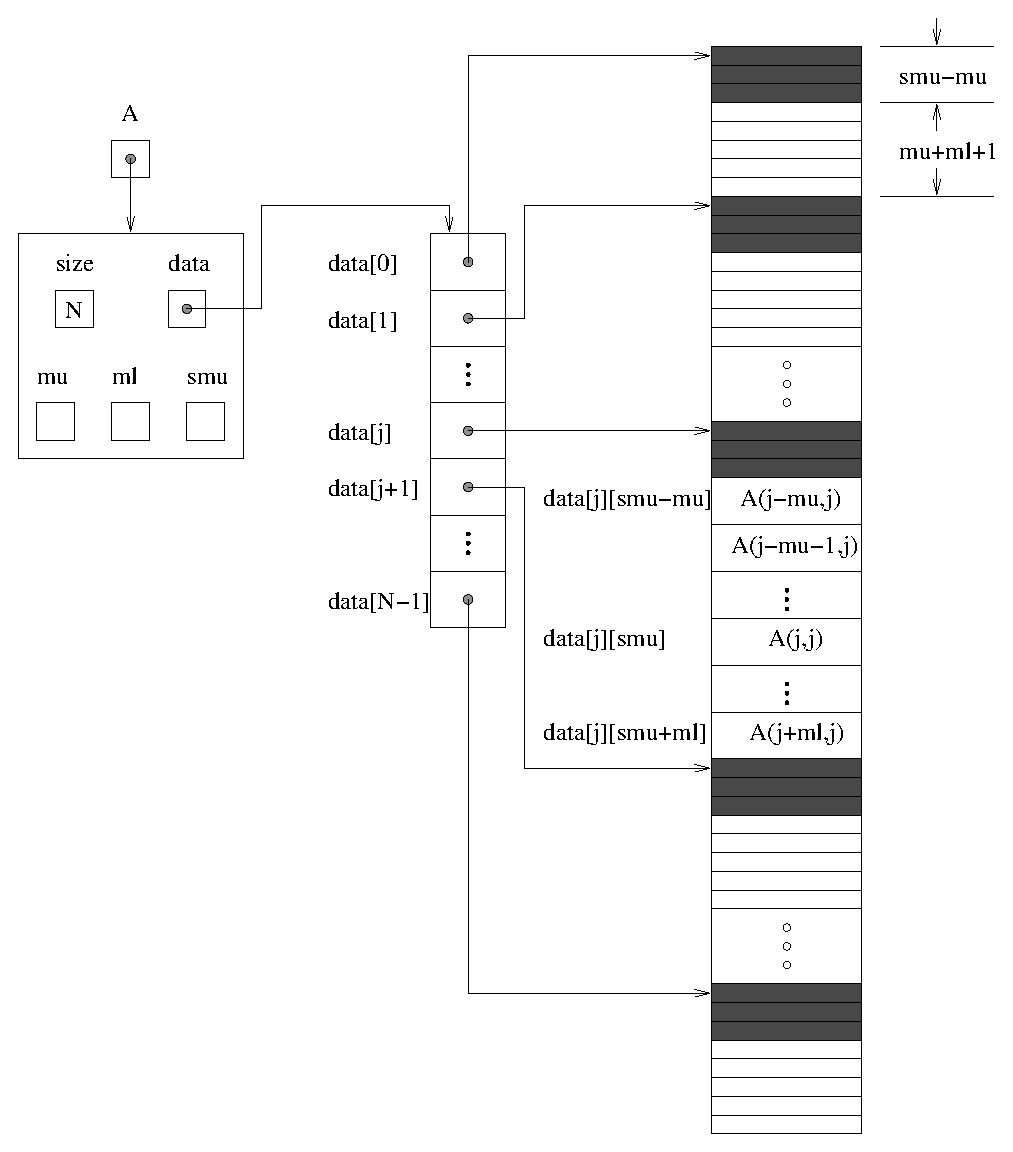
\includegraphics[width=4.5 in]{bandmat}}
\caption[Diagram of the storage for a {\sunmatband} object]
  {Diagram of the storage for the {\sunmatband} module. Here \id{A} is an
  $\id{N} \times \id{N}$ band matrix with upper and lower half-bandwidths \id{mu}
  and \id{ml}, respectively. The rows and columns of \id{A} are
  numbered from $0$ to $\id{N}-1$ and the ($i,j$)-th element of \id{A} is
  denoted \id{A(i,j)}. The greyed out areas of the underlying
  component storage are used by the associated {\sunlinsolband}
  linear solver.}\label{f:sunbandmat}
\end{figure}

\noindent The header file to include when using this module
is \id{sunmatrix/sunmatrix\_band.h}. The {\sunmatband} module
is accessible from all {\sundials} solvers \textit{without}
linking to the \newline
\id{libsundials\_sunmatrixband} module library.


% ====================================================================
\subsection{SUNMatrix\_Band accessor macros}
\label{ss:sunmat_band_macros}
% ====================================================================

The following macros are provided to access the
content of a {\sunmatband} matrix. The prefix \id{SM\_} in the names
denotes that these macros are for \emph{SUNMatrix} implementations,
and the suffix \id{\_B} denotes that these are specific to
the \emph{banded} version.
%%
\begin{itemize}

\item \ID{SM\_CONTENT\_B}

  This routine gives access to the contents of the
  banded \id{SUNMatrix}.

  The assignment \id{A\_cont} $=$ \id{SM\_CONTENT\_B(A)} sets
  \id{A\_cont} to be a pointer to the banded \id{SUNMatrix} content
  structure.

  Implementation:

  \verb|#define SM_CONTENT_B(A)     ( (SUNMatrixContent_Band)(A->content) )|

\item \ID{SM\_ROWS\_B}, \ID{SM\_COLUMNS\_B}, \ID{SM\_UBAND\_B}, \ID{SM\_LBAND\_B}, \ID{SM\_SUBAND\_B}, \ID{SM\_LDIM\_B}, and \ID{SM\_LDATA\_B}

  These macros give individual access to various lengths relevant to the
  content of a banded \id{SUNMatrix}.

  These may be used either to retrieve or to set these values.  For
  example, the assignment \id{A\_rows = SM\_ROWS\_B(A)} sets \id{A\_rows} to be
  the number of rows in the matrix \id{A}.  Similarly, the
  assignment \id{SM\_COLUMNS\_B(A) = A\_cols} sets the number of
  columns in \id{A} to equal \id{A\_cols}.

  Implementation:

  \verb|#define SM_ROWS_B(A)        ( SM_CONTENT_B(A)->M )|

  \verb|#define SM_COLUMNS_B(A)     ( SM_CONTENT_B(A)->N )|

  \verb|#define SM_UBAND_B(A)       ( SM_CONTENT_B(A)->mu )|

  \verb|#define SM_LBAND_B(A)       ( SM_CONTENT_B(A)->ml )|

  \verb|#define SM_SUBAND_B(A)      ( SM_CONTENT_B(A)->s_mu )|

  \verb|#define SM_LDIM_B(A)        ( SM_CONTENT_B(A)->ldim )|

  \verb|#define SM_LDATA_B(A)       ( SM_CONTENT_B(A)->ldata )|

\item \ID{SM\_DATA\_B} and \ID{SM\_COLS\_B}

  These macros give access to the \id{data} and \id{cols} pointers for
  the matrix entries.

  The assignment \id{A\_data = SM\_DATA\_B(A)} sets \id{A\_data} to be
  a pointer to the first component of the data array for the
  banded \id{SUNMatrix} \id{A}.  The assignment \id{SM\_DATA\_B(A) =
  A\_data} sets the data array of \id{A} to be \id{A\_data} by storing
  the pointer \id{A\_data}.

  Similarly, the assignment \id{A\_cols = SM\_COLS\_B(A)} sets \id{A\_cols} to be
  a pointer to the array of column pointers for the banded \id{SUNMatrix} \id{A}.
  The assignment \id{SM\_COLS\_B(A) = A\_cols} sets the column pointer
  array of \id{A} to be \id{A\_cols} by storing the pointer \id{A\_cols}.

  Implementation:

  \verb|#define SM_DATA_B(A)        ( SM_CONTENT_B(A)->data )|

  \verb|#define SM_COLS_B(A)        ( SM_CONTENT_B(A)->cols )|


\item \ID{SM\_COLUMN\_B}, \ID{SM\_COLUMN\_ELEMENT\_B}, and \ID{SM\_ELEMENT\_B}

  These macros give access to the individual columns and entries of
  the data array of a banded \id{SUNMatrix}.

  The assignments \id{SM\_ELEMENT\_B(A,i,j) = a\_ij} and \id{a\_ij =
  SM\_ELEMENT\_B(A,i,j)} reference the (\id{i},\id{j})-th element of the
  $\id{N} \times \id{N}$ band matrix \id{A}, where $0 \le \id{i}, \id{j} \le \id{N}-1$.
  The location (\id{i},\id{j}) should further satisfy
  \id{j}$-$\id{mu} $\le$ \id{i} $\le$ \id{j}$+$\id{ml}.

  The assignment \id{col\_j = SM\_COLUMN\_B(A,j)} sets \id{col\_j} to be
  a pointer to the diagonal element of the \id{j}-th column of the
  $\id{N} \times \id{N}$ band matrix \id{A}, $0 \le \id{j} \le \id{N}-1$.
  The type of the expression \id{SM\_COLUMN\_B(A,j)} is \id{realtype *}.
  The pointer returned by the call \id{SM\_COLUMN\_B(A,j)} can be treated as
  an array which is indexed from $-$\id{mu} to \id{ml}.

  The assignments \id{SM\_COLUMN\_ELEMENT\_B(col\_j,i,j) = a\_ij} and\\
  \id{a\_ij = SM\_COLUMN\_ELEMENT\_B(col\_j,i,j)} reference the
  (\id{i},\id{j})-th entry of the band matrix \id{A} when used in
  conjunction with \id{SM\_COLUMN\_B} to reference the \id{j}-th column
  through \id{col\_j}. The index (\id{i},\id{j}) should satisfy
  \id{j}$-$\id{mu} $\le$ \id{i} $\le$ \id{j}$+$\id{ml}.

  Implementation:

  \verb|#define SM_COLUMN_B(A,j)    ( ((SM_CONTENT_B(A)->cols)[j])+SM_SUBAND_B(A) )|

  \verb|#define SM_COLUMN_ELEMENT_B(col_j,i,j) (col_j[(i)-(j)])|

  \verb|#define SM_ELEMENT_B(A,i,j)|

  \hspace{1in} \verb|( (SM_CONTENT_B(A)->cols)[j][(i)-(j)+SM_SUBAND_B(A)] )|

\end{itemize}


% ====================================================================
\subsection{SUNMatrix\_Band functions}
\label{ss:sunmat_band_functions}
% ====================================================================

The {\sunmatband} module defines banded implementations of all matrix
operations listed in Section \ref{ss:sunmatrix_functions}. Their names are obtained
from those in Section \ref{ss:sunmatrix_functions} by appending the
suffix \id{\_Band} (e.g. \id{SUNMatCopy\_Band}).
All the standard matrix operations listed in Section \ref{ss:sunmatrix_functions} with the suffix
\id{\_Band} appended are callable via the {\F} 2003 interface by prepending an
`F' (e.g. \id{FSUNMatCopy\_Band}).

The module {\sunmatband} provides the following additional user-callable routines:
%%--------------------------------------
\sunmodfunf{SUNBandMatrix}
{
  This constructor function creates and allocates memory for a banded \id{SUNMatrix}.
  Its arguments are the matrix size, \id{N}, and the upper and lower
  half-bandwidths of the matrix, \id{mu} and \id{ml}.  The stored
  upper bandwidth is set to \id{mu+ml} to accommodate subsequent
  factorization in the {\sunlinsolband} and {\sunlinsollapband} modules.
}
{
  SUNMatrix SUNBandMatrix(sunindextype N, sunindextype mu,
  sunindextype ml)
}
%%--------------------------------------
\sunmodfun{SUNBandMatrixStorage}
{
  This constructor function creates and allocates memory for a banded \id{SUNMatrix}.
  Its arguments are the matrix size, \id{N}, the upper and lower
  half-bandwidths of the matrix, \id{mu} and \id{ml}, and the stored
  upper bandwidth, \id{smu}.  When creating a band \id{SUNMatrix},
  this value should be
  \begin{itemize}
  \item at least min(\id{N}-1,\id{mu}+\id{ml}) if the matrix will be
    used by the {\sunlinsolband} module;
  \item exactly equal to \id{mu}+\id{ml} if the matrix will be used by
    the {\sunlinsollapband} module;
  \item at least \id{mu} if used in some other manner.
  \end{itemize}
  \emph{Note: it is strongly recommended that users call the default
    constructor, \id{SUNBandMatrix}, in all standard use cases.  This
    advanced constructor is used internally within {\sundials}
    solvers, and is provided to users who require banded matrices for
    non-default purposes.}
}
{
  SUNMatrix SUNBandMatrixStorage(sunindextype N, sunindextype mu,
  \newlinefill{SUNMatrix SUNBandMatrixStorage}
  sunindextype ml, sunindextype smu)
}
%%--------------------------------------
\sunmodfun{SUNBandMatrix\_Print}
{
  This function prints the content of a banded \id{SUNMatrix} to the
  output stream specified by \id{outfile}.  Note: \id{stdout}
  or \id{stderr} may be used as arguments for \id{outfile} to print
  directly to standard output or standard error, respectively.
}
{
  void SUNBandMatrix\_Print(SUNMatrix A, FILE* outfile)
}
%%--------------------------------------
\sunmodfunf{SUNBandMatrix\_Rows}
{
  This function returns the number of rows in the banded \id{SUNMatrix}.
}
{
  sunindextype SUNBandMatrix\_Rows(SUNMatrix A)
}
%%--------------------------------------
\sunmodfunf{SUNBandMatrix\_Columns}
{
  This function returns the number of columns in the banded \id{SUNMatrix}.
}
{
  sunindextype SUNBandMatrix\_Columns(SUNMatrix A)
}
%%--------------------------------------
\sunmodfunf{SUNBandMatrix\_LowerBandwidth}
{
  This function returns the lower half-bandwidth of the banded \id{SUNMatrix}.
}
{
  sunindextype SUNBandMatrix\_LowerBandwidth(SUNMatrix A)
}
%%--------------------------------------
\sunmodfunf{SUNBandMatrix\_UpperBandwidth}
{
  This function returns the upper half-bandwidth of the banded \id{SUNMatrix}.
}
{
  sunindextype SUNBandMatrix\_UpperBandwidth(SUNMatrix A)
}
%%--------------------------------------
\sunmodfunf{SUNBandMatrix\_StoredUpperBandwidth}
{
  This function returns the stored upper half-bandwidth of the banded \id{SUNMatrix}.
}
{
  sunindextype SUNBandMatrix\_StoredUpperBandwidth(SUNMatrix A)
}
%%--------------------------------------
\sunmodfunf{SUNBandMatrix\_LDim}
{
  This function returns the length of the leading dimension of the banded \id{SUNMatrix}.
}
{
  sunindextype SUNBandMatrix\_LDim(SUNMatrix A)
}
%%--------------------------------------
\sunmodfunf{SUNBandMatrix\_Data}
{
  This function returns a pointer to the data array for the banded \id{SUNMatrix}.
}
{
  realtype* SUNBandMatrix\_Data(SUNMatrix A)
}
%%--------------------------------------
\sunmodfun{SUNBandMatrix\_Cols}
{
  This function returns a pointer to the cols array for the banded \id{SUNMatrix}.
}
{
  realtype** SUNBandMatrix\_Cols(SUNMatrix A)
}
%%--------------------------------------
\sunmodfunf{SUNBandMatrix\_Column}
{
  This function returns a pointer to the diagonal entry of the j-th
  column of the banded \id{SUNMatrix}.  The resulting pointer should
  be indexed over the range $-$\id{mu} to \id{ml}.
}
{
  realtype* SUNBandMatrix\_Column(SUNMatrix A, sunindextype j)
}
%%
%%------------------------------------
%%
\paragraph{\bf Notes}

\begin{itemize}

\item
  When looping over the components of a banded \id{SUNMatrix} \id{A},
  the most efficient approaches are to:
  \begin{itemize}
    \item First obtain the component array via \id{A\_data = SM\_DATA\_B(A)} or\\
    \id{A\_data = SUNBandMatrix\_Data(A)} and then
    access \id{A\_data[i]} within the loop.

    \item First obtain the array of column pointers via \id{A\_cols = SM\_COLS\_B(A)} or\\
    \id{A\_cols = SUNBandMatrix\_Cols(A)}, and then
    access \id{A\_cols[j][i]} within the loop.

    \item Within a loop over the columns, access the column pointer via\\
    \id{A\_colj = SUNBandMatrix\_Column(A,j)} and then to access the
    entries within that column using \id{SM\_COLUMN\_ELEMENT\_B(A\_colj,i,j)}.
  \end{itemize}
  All three of these are more efficient than
  using \id{SM\_ELEMENT\_B(A,i,j)} within a double loop.

\item
  {\warn} Within the \id{SUNMatMatvec\_Band} routine, internal
  consistency checks are performed to ensure that the matrix is called
  with consistent {\nvector} implementations.  These are currently
  limited to: {\nvecs}, {\nvecopenmp}, and {\nvecpthreads}.  As additional
  compatible vector implementations are added to {\sundials}, these
  will be included within this compatibility check.

\end{itemize}


% ====================================================================
\subsection{SUNMatrix\_Band Fortran interfaces}
\label{ss:sunmat_band_fortran}
% ====================================================================

The {\sunmatband} module provides a {\F} 2003 module as well as {\F} 77
style interface functions for use from {\F} applications.

\subsubsection*{FORTRAN 2003 interface module}
The \ID{fsunmatrix\_band\_mod} {\F} module defines interfaces to most
{\sunmatband} {\CC} functions using the intrinsic \id{iso\_c\_binding}
module which provides a standardized mechanism for interoperating with {\CC}. As
noted in the {\CC} function descriptions above, the interface functions are
named after the corresponding {\CC} function, but with a leading `F'. For
example, the function \id{SUNBandMatrix} is interfaced as
\id{FSUNBandMatrix}.

The {\F} 2003 {\sunmatband} interface module can be accessed with the \id{use}
statement, i.e. \id{use fsunmatrix\_band\_mod}, and linking to the library
\id{libsundials\_fsunmatrixband\_mod}.{\em lib} in addition to the {\CC} library.
For details on where the library and module file
\id{fsunmatrix\_band\_mod.mod} are installed see Appendix \ref{c:install}.
We note that the module is accessible from the {\F} 2003 {\sundials} integrators
\textit{without} separately linking to the
\id{libsundials\_fsunmatrixband\_mod} library.

\subsubsection*{FORTRAN 77 interface functions}
For solvers that include a {\F} interface module, the {\sunmatband}
module also includes the {\F}-callable
function \id{FSUNBandMatInit(code, N, mu, ml, ier)} to initialize
this {\sunmatband} module for a given {\sundials} solver.
Here \id{code} is an integer input solver id (1 for {\cvode}, 2 for {\ida}, 3
for {\kinsol}, 4 for {\arkode}); \id{N}, \id{mu}, and \id{ml}
are the corresponding band matrix construction arguments (declared
to match C type \id{long int}); and \id{ier} is an error return flag
equal to 0 for success and -1 for failure. Both \id{code} and \id{ier}
are declared to match C type \id{int}. Additionally, when using
{\arkode} with a non-identity mass matrix, the {\F}-callable
function \id{FSUNBandMassMatInit(N, mu, ml, ier)} initializes
this {\sunmatband} module for storing the mass matrix.

%% This is a shared SUNDIALS TEX file with a description of the
%% sparse sunmatrix implementation
%%
\section{The SUNMatrix\_Sparse implementation}\label{ss:sunmat_sparse}

The sparse implementation of the {\sunmatrix} module provided with
{\sundials}, {\sunmatsparse}, is designed to work with either
\emph{compressed-sparse-column} (CSC) or \emph{compressed-sparse-row}
(CSR) sparse matrix formats.  To this end, it defines the {\em
content} field of \id{SUNMatrix} to be the following structure:
%%
\begin{verbatim} 
struct _SUNMatrixContent_Sparse {
  sunindextype M;
  sunindextype N;
  sunindextype NNZ;
  sunindextype NP;
  realtype *data;
  int sparsetype;
  sunindextype *indexvals;
  sunindextype *indexptrs;
  /* CSC indices */
  sunindextype **rowvals;
  sunindextype **colptrs;
  /* CSR indices */
  sunindextype **colvals;
  sunindextype **rowptrs;
};
\end{verbatim}
%%
A diagram of the underlying data representation for a
CSC matrix is shown in Figure \ref{f:sparsemat} (the CSR format is
similar).  A more complete description of the parts of
this \emph{content} field is given below: 
\begin{args}[sparsetype]
  \item[M]  - number of rows
  \item[N]  - number of columns
  \item[NNZ]  - maximum number of nonzero entries in the matrix
    (allocated length of \id{data} and \id{indexvals} arrays)
  \item[NP]  - number of index pointers (e.g. number of column pointers for 
    CSC matrix). For CSC matrices $\id{NP}=\id{N}$, and for CSR
    matrices $\id{NP}=\id{M}$. This value is set automatically based
    the input for \verb|sparsetype|.
  \item[data]  - pointer to a contiguous block of \id{realtype}
    variables (of length \id{NNZ}), containing the values of the
    nonzero entries in the matrix
  \item[sparsetype]  - type of the sparse matrix (\id{CSC\_MAT} or \id{CSR\_MAT})
  \item[indexvals] - pointer to a contiguous block of \id{int} variables
    (of length \id{NNZ}), containing the row indices (if CSC) or column
   indices (if CSR) of each nonzero matrix entry held in \id{data}
  \item[indexptrs]  - pointer to a contiguous block of \id{int}
    variables (of length \id{NP+1}). For CSC matrices each 
    entry provides the index of the first column entry into the 
    \id{data} and \id{indexvals} arrays, e.g. if \id{indexptr[3]=7}, then 
    the first nonzero entry in the fourth column of the matrix is 
    located in \id{data[7]}, and is located in row \id{indexvals[7]} of the 
    matrix.  The last entry contains the total number of nonzero values in 
    the matrix and hence points one past the end of the active data in the 
    \id{data} and \id{indexvals} arrays. For CSR matrices, each entry provides 
    the index of the first row entry into the \id{data} and \id{indexvals} 
    arrays.
\end{args}
\noindent The following pointers are added to the \id{SlsMat} type for
  user convenience, to provide a more intuitive interface to the CSC
  and CSR sparse matrix data structures. They are set automatically
  when creating a sparse {\sunmatrix}, based on the sparse matrix storage
  type.  
\begin{args}[colptrs]
  \item[rowvals] - pointer to \verb|indexvals| when \id{sparsetype} is \id{CSC\_MAT},
    otherwise set to \verb|NULL|.
  \item[colptrs] - pointer to \verb|indexptrs| when \id{sparsetype} is \id{CSC\_MAT},
    otherwise set to \verb|NULL|.
  \item[colvals] - pointer to \verb|indexvals| when \id{sparsetype} is \id{CSR\_MAT},
    otherwise set to \verb|NULL|.
  \item[rowptrs] - pointer to \verb|indexptrs| when \id{sparsetype} is \id{CSR\_MAT},
    otherwise set to \verb|NULL|.
\end{args}
For example, the $5\times 4$ CSC matrix
\[
  \left[\begin{array}{cccc} 
     0 & 3 & 1 & 0\\
     3 & 0 & 0 & 2\\
     0 & 7 & 0 & 0\\
     1 & 0 & 0 & 9\\
     0 & 0 & 0 & 5
  \end{array}\right]
\]
could be stored in this structure as either
\begin{verbatim}
  M = 5;
  N = 4;
  NNZ = 8;
  NP = N;
  data = {3.0, 1.0, 3.0, 7.0, 1.0, 2.0, 9.0, 5.0};
  sparsetype = CSC_MAT;
  indexvals = {1, 3, 0, 2, 0, 1, 3, 4};
  indexptrs = {0, 2, 4, 5, 8};
\end{verbatim}
or 
\begin{verbatim}
  M = 5;
  N = 4;
  NNZ = 10;
  NP = N;
  data = {3.0, 1.0, 3.0, 7.0, 1.0, 2.0, 9.0, 5.0, *, *};
  sparsetype = CSC_MAT;
  indexvals = {1, 3, 0, 2, 0, 1, 3, 4, *, *};
  indexptrs = {0, 2, 4, 5, 8};
\end{verbatim}
where the first has no unused space, and the second has additional
storage (the entries marked with \texttt{*} may contain any values).
Note in both cases that the final value in \id{indexptrs} is $8$,
indicating the total number of nonzero entries in the matrix.

Similarly, in CSR format, the same matrix could be stored as
\begin{verbatim}
  M = 5;
  N = 4;
  NNZ = 8;
  NP = N;
  data = {3.0, 1.0, 3.0, 2.0, 7.0, 1.0, 9.0, 5.0};
  sparsetype = CSR_MAT;
  indexvals = {1, 2, 0, 3, 1, 0, 3, 3};
  indexptrs = {0, 2, 4, 5, 7, 8};
\end{verbatim}

%%
%%--------------------------------------------
%%
\begin{figure}
\centerline{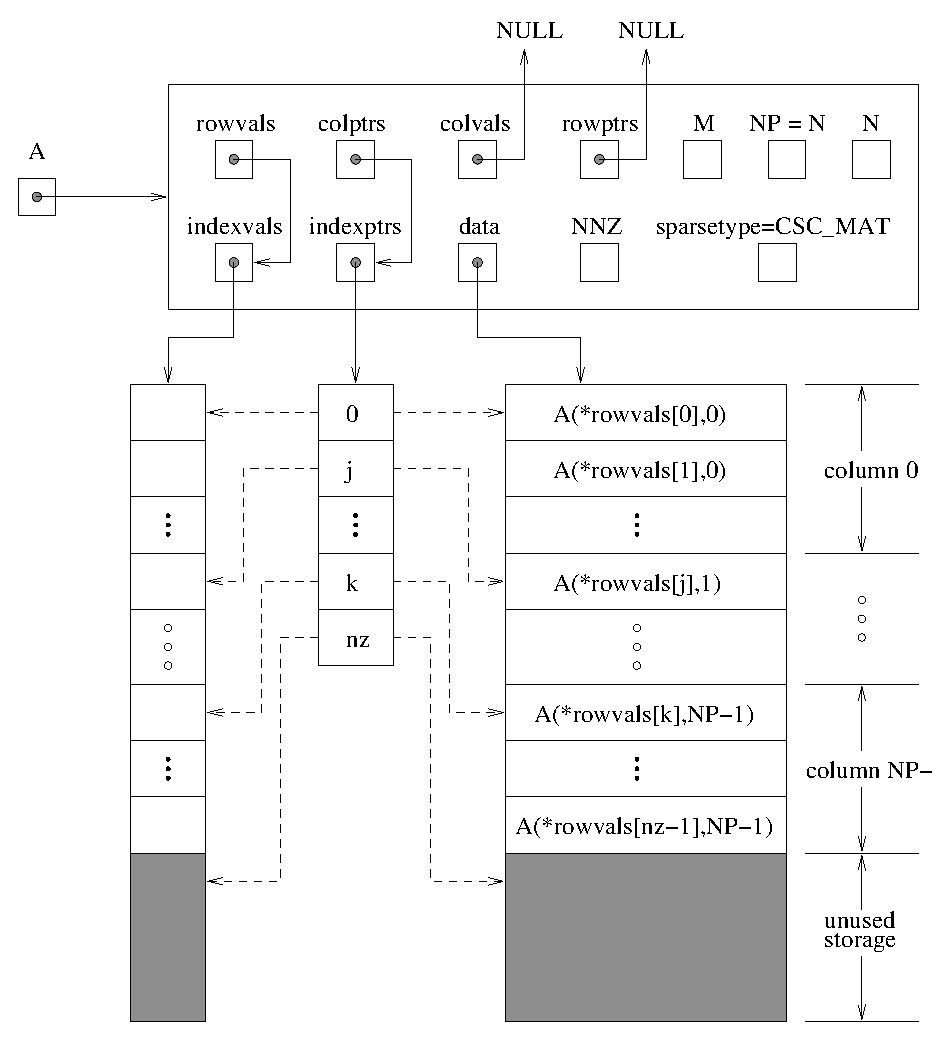
\includegraphics[width=4.5 in]{cscmat}}
\caption[Diagram of the storage for a compressed-sparse-column matrix] 
  {Diagram of the storage for a compressed-sparse-column
  matrix. Here \id{A} is an $\id{M} \times \id{N}$ sparse matrix with storage
  for up to \id{NNZ} nonzero entries (the allocated length of
  both \id{data} and \id{indexvals}).  The entries in \id{indexvals}
  may assume values from $0$ to $\id{M}-1$, corresponding to the row index
  (zero-based) of each nonzero value.  The entries in \id{data} contain
  the values of the nonzero entries, with the row $i$, column $j$
  entry of \id{A} (again, zero-based) denoted as \id{A(i,j)}.
  The \id{indexptrs} array contains $\id{N}+1$ entries; the first $\id{N}$
  denote the starting index of each column within the \id{indexvals}
  and \id{data} arrays, while the final entry points one past the
  final nonzero entry.  Here, although \id{NNZ} values are allocated,
  only \id{nz} are actually filled in; the greyed-out portions
  of \id{data} and \id{indexvals} indicate extra allocated
  space.}\label{f:sparsemat} 
\end{figure}

\noindent The header file to include when using this module 
is \id{sunmatrix/sunmatrix\_sparse.h}. The {\sunmatsparse} module
is accessible from all {\sundials} solvers \textit{without}
linking to the \\
\id{libsundials\_sunmatrixsparse} module library.


% ====================================================================
\subsection{SUNMatrix\_Sparse accessor macros}
\label{ss:sunmat_sparse_macros}
% ====================================================================

The following macros are provided to access the
content of a {\sunmatsparse} matrix. The prefix \id{SM\_} in the names
denotes that these macros are for \emph{SUNMatrix} implementations,
and the suffix \id{\_S} denotes that these are specific to
the \emph{sparse} version.
%%
\begin{itemize}

\item \ID{SM\_CONTENT\_S}
    
  This routine gives access to the contents of the
  sparse \id{SUNMatrix}.
  
  The assignment \id{A\_cont} $=$ \id{SM\_CONTENT\_S(A)} sets           
  \id{A\_cont} to be a pointer to the sparse \id{SUNMatrix} content  
  structure.                                             
                                                            
  Implementation: 
  
  \verb|#define SM_CONTENT_S(A)     ( (SUNMatrixContent_Sparse)(A->content) )|
  
\item \ID{SM\_ROWS\_S}, \ID{SM\_COLUMNS\_S}, \ID{SM\_NNZ\_S}, \ID{SM\_NP\_S}, and \ID{SM\_SPARSETYPE\_S}

  These macros give individual access to various lengths relevant to the
  content of a sparse \id{SUNMatrix}.
                                                               
  These may be used either to retrieve or to set these values.  For
  example, the assignment \id{A\_rows = SM\_ROWS\_S(A)} sets \id{A\_rows} to be
  the number of rows in the matrix \id{A}.  Similarly, the
  assignment \id{SM\_COLUMNS\_S(A) = A\_cols} sets the number of
  columns in \id{A} to equal \id{A\_cols}.
  
  Implementation: 
  
  \verb|#define SM_ROWS_S(A)        ( SM_CONTENT_S(A)->M )|

  \verb|#define SM_COLUMNS_S(A)     ( SM_CONTENT_S(A)->N )|

  \verb|#define SM_NNZ_S(A)         ( SM_CONTENT_S(A)->NNZ )|

  \verb|#define SM_NP_S(A)          ( SM_CONTENT_S(A)->NP )|

  \verb|#define SM_SPARSETYPE_S(A)  ( SM_CONTENT_S(A)->sparsetype )|


\item \ID{SM\_DATA\_S}, \ID{SM\_INDEXVALS\_S}, and \ID{SM\_INDEXPTRS\_S}
                                                            
  These macros give access to the \id{data} and index arrays for
  the matrix entries.

  The assignment \id{A\_data = SM\_DATA\_S(A)} sets \id{A\_data} to be     
  a pointer to the first component of the data array for the
  sparse \id{SUNMatrix} \id{A}.  The assignment \id{SM\_DATA\_S(A) =
  A\_data} sets the data array of \id{A} to be \id{A\_data} by storing
  the pointer \id{A\_data}. 
  
  Similarly, the assignment \id{A\_indexvals = SM\_INDEXVALS\_S(A)}
  sets \id{A\_indexvals} to be a pointer to the array of index values
  (i.e.~row indices for a CSC matrix, or column indices for a CSR
  matrix) for the sparse \id{SUNMatrix} \id{A}.  The
  assignment \id{A\_indexptrs = SM\_INDEXPTRS\_S(A)}
  sets \id{A\_indexptrs} to be a pointer to the array of index
  pointers (i.e.~the starting indices in the data/indexvals arrays for
  each row or column in CSR or CSC formats, respectively).
  
  Implementation:

  \verb|#define SM_DATA_S(A)        ( SM_CONTENT_S(A)->data )|

  \verb|#define SM_INDEXVALS_S(A)   ( SM_CONTENT_S(A)->indexvals )|

  \verb|#define SM_INDEXPTRS_S(A)   ( SM_CONTENT_S(A)->indexptrs )|

\end{itemize}


% ====================================================================
\subsection{SUNMatrix\_Sparse functions}
\label{ss:sunmat_sparse_functions}
% ====================================================================

The {\sunmatsparse} module defines sparse implementations of all matrix
operations listed in Section \ref{ss:sunmatrix_functions}. Their names are obtained
from those in Section \ref{ss:sunmatrix_functions} by appending the
suffix \id{\_Sparse} (e.g. \id{SUNMatCopy\_Sparse}). 
All the standard matrix operations listed in Section \ref{ss:sunmatrix_functions} with the suffix
\id{\_Sparse} appended are callable via the {\F} 2003 interface by prepending an
`F' (e.g. \id{FSUNMatCopy\_Sparse}).

The module {\sunmatsparse} provides the following additional
user-callable routines: 
%%--------------------------------------
\sunmodfunf{SUNSparseMatrix}
{
  This function creates and allocates memory for a sparse \id{SUNMatrix}.
  Its arguments are the number of rows and columns of the
  matrix, \id{M} and \id{N}, the maximum number of nonzeros to be
  stored in the matrix, \id{NNZ}, and a flag \id{sparsetype}
  indicating whether to use CSR or CSC format (valid arguments
  are \id{CSR\_MAT} or \id{CSC\_MAT}). 
}
{
  SUNMatrix SUNSparseMatrix(sunindextype M, sunindextype N,
  \newlinefill{SUNMatrix SUNSparseMatrix}
  sunindextype NNZ, int sparsetype)
}
%%--------------------------------------
\sunmodfunf{SUNSparseFromDenseMatrix}
{
  This function creates a new sparse matrix from an existing dense
  matrix by copying all values with magnitude larger than \id{droptol}
  into the sparse matrix structure.

  Requirements:
  \begin{itemize}
  \item \id{A} must have type \id{SUNMATRIX\_DENSE};
  \item \id{droptol} must be non-negative;
  \item \id{sparsetype} must be either \id{CSC\_MAT} or \id{CSR\_MAT}.
  \end{itemize}
  The function returns NULL if any requirements are violated, or if
  the matrix storage request cannot be satisfied. 
}
{
  SUNMatrix SUNSparseFromDenseMatrix(SUNMatrix A, realtype droptol,
  \newlinefill{SUNMatrix SUNSparseFromDenseMatrix}
  int sparsetype);
}
%%--------------------------------------
\sunmodfunf{SUNSparseFromBandMatrix}
{
  This function creates a new sparse matrix from an existing band
  matrix by copying all values with magnitude larger than \id{droptol}
  into the sparse matrix structure.

  Requirements:
  \begin{itemize}
  \item \id{A} must have type \id{SUNMATRIX\_BAND};
  \item \id{droptol} must be non-negative;
  \item \id{sparsetype} must be either \id{CSC\_MAT} or \id{CSR\_MAT}.
  \end{itemize}
  The function returns NULL if any requirements are violated, or if
  the matrix storage request cannot be satisfied. 
}
{
  SUNMatrix SUNSparseFromBandMatrix(SUNMatrix A, realtype droptol,
  \newlinefill{SUNMatrix SUNSparseFromBandMatrix}
  int sparsetype);
}
%%--------------------------------------
\sunmodfunf{SUNSparseMatrix\_Realloc}
{
  This function reallocates internal storage arrays in a sparse matrix
  so that the resulting sparse matrix has no wasted space (i.e.~the
  space allocated for nonzero entries equals the actual number of
  nonzeros, \id{indexptrs[NP]}). Returns 0 on success and 
  1 on failure (e.g.~if the input matrix is not sparse).
}
{
  int SUNSparseMatrix\_Realloc(SUNMatrix A)
}
%%--------------------------------------
\sunmodfunf{SUNSparseMatrix\_Reallocate}
{
  This function reallocates internal storage arrays in a sparse matrix
  so that the resulting sparse matrix has storage for a specified
  number of nonzeros. Returns 0 on success and 
  1 on failure (e.g.~if the input matrix is not sparse or if NNZ is
  negative). 
}
{
  int SUNSparseMatrix\_Reallocate(SUNMatrix A, sunindextype NNZ)
}
%%--------------------------------------
\sunmodfun{SUNSparseMatrix\_Print}
{
  This function prints the content of a sparse \id{SUNMatrix} to the
  output stream specified by \id{outfile}.  Note: \id{stdout}
  or \id{stderr} may be used as arguments for \id{outfile} to print
  directly to standard output or standard error, respectively.
}
{
  void SUNSparseMatrix\_Print(SUNMatrix A, FILE* outfile)
}
%%--------------------------------------
\sunmodfunf{SUNSparseMatrix\_Rows}
{
  This function returns the number of rows in the sparse \id{SUNMatrix}.
}
{
  sunindextype SUNSparseMatrix\_Rows(SUNMatrix A)
}
%%--------------------------------------
\sunmodfunf{SUNSparseMatrix\_Columns}
{
  This function returns the number of columns in the sparse \id{SUNMatrix}.
}
{
  sunindextype SUNSparseMatrix\_Columns(SUNMatrix A)
}
%%--------------------------------------
\sunmodfunf{SUNSparseMatrix\_NNZ}
{
  This function returns the number of entries allocated for nonzero
  storage for  the sparse matrix \id{SUNMatrix}.
}
{
  sunindextype SUNSparseMatrix\_NNZ(SUNMatrix A)
}
%%--------------------------------------
\sunmodfunf{SUNSparseMatrix\_NP}
{
  This function returns the number of columns/rows for the
  sparse \id{SUNMatrix}, depending on whether the matrix uses CSC/CSR
  format, respectively.  The \id{indexptrs} array has \id{NP+1} entries.
}
{
  sunindextype SUNSparseMatrix\_NP(SUNMatrix A)
}
%%--------------------------------------
\sunmodfunf{SUNSparseMatrix\_SparseType}
{
  This function returns the storage type (\id{CSR\_MAT}
  or \id{CSC\_MAT}) for the sparse \id{SUNMatrix}.
}
{
  int SUNSparseMatrix\_SparseType(SUNMatrix A)
}
%%--------------------------------------
\sunmodfunf{SUNSparseMatrix\_Data}
{
  This function returns a pointer to the data array for the
  sparse \id{SUNMatrix}. 
}
{
  realtype* SUNSparseMatrix\_Data(SUNMatrix A)
}
%%--------------------------------------
\sunmodfunf{SUNSparseMatrix\_IndexValues}
{
  This function returns a pointer to index value array for the sparse
  \id{SUNMatrix}: for CSR format this is the column index for each nonzero
  entry, for CSC format this is the row index for each nonzero entry.
}
{
  sunindextype* SUNSparseMatrix\_IndexValues(SUNMatrix A)
}
%%--------------------------------------
\sunmodfunf{SUNSparseMatrix\_IndexPointers}
{
  This function returns a pointer to the index pointer array for the
  sparse \id{SUNMatrix}: for CSR format this is the location of the first
  entry of each row in the \id{data} and \id{indexvalues} arrays, for
  CSC format this is the location of the first entry of each column.
}
{
  sunindextype* SUNSparseMatrix\_IndexPointers(SUNMatrix A)
}
%%
%%------------------------------------
%%
{\warn} Within the \id{SUNMatMatvec\_Sparse} routine, internal
consistency checks are performed to ensure that the matrix is called
with consistent {\nvector} implementations.  These are currently
limited to: {\nvecs}, {\nvecopenmp}, {\nvecpthreads}, and {\nveccuda}
when using managed memory.  As additional compatible vector implementations
are added to {\sundials}, these will be included within this compatibility check. 


% ====================================================================
\subsection{SUNMatrix\_Sparse Fortran interfaces}
\label{ss:sunmat_sparse_fortran}
% ====================================================================

The {\sunmatsparse} module provides a {\F} 2003 module as well as {\F} 77
style interface functions for use from {\F} applications.

\subsubsection*{FORTRAN 2003 interface module}
The \ID{fsunmatrix\_sparse\_mod} {\F} module defines interfaces to most
{\sunmatsparse} {\CC} functions using the intrinsic \id{iso\_c\_binding}
module which provides a standardized mechanism for interoperating with {\CC}. As
noted in the {\CC} function descriptions above, the interface functions are
named after the corresponding {\CC} function, but with a leading `F'. For
example, the function \id{SUNSparseMatrix} is interfaced as
\id{FSUNSparseMatrix}.

The {\F} 2003 {\sunmatsparse} interface module can be accessed with the \id{use}
statement, i.e. \id{use fsunmatrix\_sparse\_mod}, and linking to the library
\id{libsundials\_fsunmatrixsparse\_mod}.{\em lib} in addition to the {\CC} library.
For details on where the library and module file
\id{fsunmatrix\_sparse\_mod.mod} are installed see Appendix \ref{c:install}.
We note that the module is accessible from the {\F} 2003 {\sundials} integrators
\textit{without} separately linking to the
\id{libsundials\_fsunmatrixsparse\_mod} library.

\subsubsection*{FORTRAN 77 interface functions}
For solvers that include a Fortran interface module, the {\sunmatsparse}
module also includes the Fortran-callable
function \id{FSUNSparseMatInit(code, M, N, NNZ, sparsetype, ier)} to
initialize this {\sunmatsparse} module for a given {\sundials} solver.
Here \id{code} is an integer input for the solver id (1 for {\cvode},
2 for {\ida}, 3 for {\kinsol}, 4 for {\arkode}); \id{M}, \id{N}
and \id{NNZ} are the corresponding sparse matrix construction
arguments (declared to match C type \id{long
int}); \id{sparsetype} is an integer flag indicating the sparse
storage type (0 for CSC, 1 for CSR); and \id{ier} is an error return
flag equal to 0 for success and -1 for failure. Each of \id{code},
\id{sparsetype} and \id{ier} are declared so as to match C
type \id{int}. Additionally, when using {\arkode} with a non-identity
mass matrix, the Fortran-callable
function \id{FSUNSparseMassMatInit(M, N, NNZ, sparsetype, ier)} 
initializes this {\sunmatsparse} module for storing the mass matrix.

%% This is a shared SUNDIALS TEX file with a description of the
%% SuperLU_DIST SLUNRloc SUNMatrix implementation
%%
\section{The SUNMatrix\_SLUNRloc implementation}\label{ss:sunmat_slunrloc}

The {\sunmatslunrloc} implementation of the {\sunmatrix} module provided with
{\sundials} is an adapter for the \id{SuperMatrix} structure provided by the
{\superludist} sparse matrix factorization and solver library written by
X. Sherry Li \cite{SuperLUDIST_site,GDL:07,LD:03,SLUUG:99}.
It is designed to be used with the {\sunlinsolsludist} linear solver
discussed in Section~\ref{ss:sunlinsol_sludist}. To this end, it defines the
{\em content} field of \id{SUNMatrix} to be the following structure:
%%
\begin{verbatim}
struct _SUNMatrixContent_SLUNRloc {
  booleantype   own_data;
  gridinfo_t    *grid;
  sunindextype  *row_to_proc;
  pdgsmv_comm_t *gsmv_comm;
  SuperMatrix   *A_super;
  SuperMatrix   *ACS_super;
};
\end{verbatim}
%%

A more complete description of the this \emph{content} field is given below:

\begin{description}
  \item[own\_data] - a flag which indicates if the SUNMatrix is responsible for freeing
    \id{A\_super}
  \item[grid] - pointer to the {\superludist} structure that stores the 2D process grid
  \item[row\_to\_proc] - a mapping between the rows in the matrix and the process it
    resides on; will be \id{NULL} until the \id{SUNMatMatvecSetup} routine is called
  \item[gsmv\_comm] - pointer to the {\superludist} structure that stores the
    communication information needed for matrix-vector multiplication; will be
    \id{NULL} until the \id{SUNMatMatvecSetup} routine is called
  \item[A\_super] - pointer to the underlying {\superludist} \id{SuperMatrix} with
      \id{Stype = SLU\_NR\_loc, Dtype = SLU\_D, Mtype = SLU\_GE}; must have the
      full diagonal present to be used with \id{SUNMatScaleAddI} routine
  \item[ACS\_super] - a column-sorted version of the matrix needed to perform matrix-vector
    multiplication; will be \id{NULL} until the routine \id{SUNMatMatvecSetup}
    routine is called
\end{description}

\noindent The header file to include when using this module
is \id{sunmatrix/sunmatrix\_slunrloc.h}. The installed module
library to link to is \id{libsundials\_sunmatrixslunrloc.\textit{lib}}
where \id{\em.lib} is typically \id{.so} for shared libraries and
\id{.a} for static libraries.


% ====================================================================
\subsection{SUNMatrix\_SLUNRloc functions}
\label{ss:sunmat_slunrloc_functions}
% ====================================================================

The module {\sunmatslunrloc} provides the following user-callable routines:
%%--------------------------------------
%%
\ucfunction{SUNMatrix\_SLUNRloc}
{
  A = SUNMatrix\_SLUNRloc(Asuper, grid);
}
{
  The function \ID{SUNMatrix\_SLUNRloc} creates and allocates memory for a
  {\sunmatslunrloc} object.
}
{
  \begin{args}
  \item[Asuper] (\id{SuperMatrix*})
      a fully-allocated {\superludist} \id{SuperMatrix} that the SUNMatrix will
      wrap; must have \id{Stype = SLU\_NR\_loc, Dtype = SLU\_D, Mtype = SLU\_GE}
      to be compatible
  \item[grid] (\id{gridinfo\_t*}) the initialized {\superludist} 2D process grid structure
  \end{args}
}
{
  a \id{SUNMatrix} object if \id{Asuper} is compatible else \id{NULL}
}
{
}

\ucfunction{SUNMatrix\_SLUNRloc\_Print}
{
  SUNMatrix\_SLUNRloc\_Print(A, fp);
}
{
  The function \ID{SUNMatrix\_SLUNRloc\_Print} prints the underlying
  \id{SuperMatrix} content.
}
{
  \begin{args}
  \item[A] (\id{SUNMatrix}) the matrix to print
  \item[fp] (\id{FILE}) the file pointer used for printing
  \end{args}
}
{
  \id{void}
}
{
}

\ucfunction{SUNMatrix\_SLUNRloc\_SuperMatrix}
{
  Asuper = SUNMatrix\_SLUNRloc\_SuperMatrix(A);
}
{
  The function \ID{SUNMatrix\_SLUNRloc\_SuperMatrix} provides access
  to the underlying {\superludist} \id{SuperMatrix} of \id{A}.
}
{
  \begin{args}
  \item[A] (\id{SUNMatrix}) the matrix to access
  \end{args}
}
{
  \id{SuperMatrix*}
}
{
}

\ucfunction{SUNMatrix\_SLUNRloc\_ProcessGrid}
{
  grid = SUNMatrix\_SLUNRloc\_ProcessGrid(A);
}
{
  The function \ID{SUNMatrix\_SLUNRloc\_ProcessGrid} provides access
  to the {\superludist} \id{gridinfo\_t} structure associated with \id{A}.
}
{
  \begin{args}
  \item[A] (\id{SUNMatrix}) the matrix to access
  \end{args}
}
{
  \id{gridinfo\_t*}
}
{
}

\ucfunction{SUNMatrix\_SLUNRloc\_OwnData}
{
  does\_own\_data = SUNMatrix\_SLUNRloc\_OwnData(A);
}
{
  The function \ID{SUNMatrix\_SLUNRloc\_OwnData} returns true if the \id{SUNMatrix}
  object is responsible for freeing \id{A\_super}, otherwise it returns false.
}
{
  \begin{args}
  \item[A] (\id{SUNMatrix}) the matrix to access
  \end{args}
}
{
  \id{booleantype}
}
{
}

The {\sunmatslunrloc} module defines implementations of all generic \id{SUNMatrix} operations
listed in Section \ref{ss:sunmatrix_functions}:

\begin{itemize}
  \item \id{SUNMatGetID\_SLUNRloc} - returns \id{SUNMATRIX\_SLUNRLOC}
  \item \id{SUNMatClone\_SLUNRloc}
  \item \id{SUNMatDestroy\_SLUNRloc}
  \item \id{SUNMatSpace\_SLUNRloc} - this only returns information for the storage within the
    matrix interface, i.e. storage for \id{row\_to\_proc}
  \item \id{SUNMatZero\_SLUNRloc}
  \item \id{SUNMatCopy\_SLUNRloc}
  \item \id{SUNMatScaleAdd\_SLUNRloc} - performs $A = cA + B$, but $A$ and $B$ must have the same sparsity pattern 
  \item \id{SUNMatScaleAddI\_SLUNRloc} - performs $A = cA + I$, but the diagonal of $A$ must be present
  \item \id{SUNMatMatvecSetup\_SLUNRloc} - initializes the {\superludist} parallel communication
    structures needed to perform a matrix-vector product; only needs to be called before the
    first call to \id{SUNMatMatvec} or if the matrix changed since the last setup
  \item \id{SUNMatMatvec\_SLUNRloc}
\end{itemize}

%%------------------------------------
%%
{\warn} The {\sunmatslunrloc} module requires that the complete diagonal, i.e. nonzeros and zeros,
is present in order to use the \id{SUNMatScaleAddI} operation.

% % ====================================================================
% \subsection{SUNMatrix\_SLUNRloc Fortran interfaces}
% \label{ss:sunmat_slunrloc_fortran}
% % ====================================================================

% The {\sunmatslunrloc} module provides a {\F} 2003 module as well as {\F} 77
% style interface functions for use from {\F} applications.

% \subsubsection*{FORTRAN 2003 interface module}
% The \ID{fsunmatrix\_slunrloc\_mod} {\F} module defines interfaces to most
% {\sunmatslunrloc} {\CC} functions using the intrinsic \id{iso\_c\_binding}
% module which provides a standardized mechanism for interoperating with {\CC}. As
% noted in the {\CC} function descriptions above, the interface functions are
% named after the corresponding {\CC} function, but with a leading `F'. For
% example, the function \id{SUNMatrix\_SLUNRloc} is interfaced as
% \id{FSUNMatrix\_SLUNRloc}.

% The {\F} 2003 {\sunmatslunrloc} interface module can be accessed with the \id{use}
% statement, i.e. \id{use fsunmatrix\_slunrloc\_mod}, and linking to the library
% \id{libsundials\_fsunmatrixslunrloc\_mod}.{\em lib} in addition to the {\CC} library.
% For details on where the library and module file \id{fsunmatrix\_slunrloc\_mod.mod}
% are installed see Appendix \ref{c:install}.



\clearemptydoublepage
%===============================================================
% Description of the SUNLinearSolver Concept
%===================================================================================
\chapter{Description of the SUNLinearSolver module}\label{s:sunlinsol}
%===================================================================================
\index{SUNLinearSolver@\texttt{SUNLinearSolver} module}
% This is a shared SUNDIALS TEX file with description of
% the generic sunlinsol abstraction
%
For problems that involve the solution of linear systems of equations,
the {\sundials} packages operate using generic linear solver modules
defined through the {\sunlinsol} API.  This allows {\sundials}
packages to utilize any valid {\sunlinsol} implementation that provides
a set of required functions.  These functions can be divided into
three categories.  The first are the core linear solver functions.  The
second group consists of ``set'' routines to supply the linear solver object
with functions provided by the {\sundials} package, or for modification
of solver parameters.  The last group consists of ``get'' routines for
retrieving artifacts (statistics, residual vectors, etc.) from the
linear solver.  All of these functions are defined in the header file
\Id{sundials/sundials\_linearsolver.h}.

The implementations provided with {\sundials} work in coordination
with the {\sundials} generic {\nvector} and {\sunmatrix} modules to
provide a set of compatible data structures and solvers for the
solution of linear systems using direct or iterative (matrix-based or matrix-free)
methods.  Moreover, advanced users can provide a customized
\Id{SUNLinearSolver} implementation to any {\sundials} package,
particularly in cases where they provide their own {\nvector} and/or
{\sunmatrix} modules.

Historically, the {\sundials} packages have been designed to specifically
leverage the use of either \emph{direct linear solvers} or matrix-free,
\emph{scaled, preconditioned, iterative linear solvers}.  However, user-supplied
implementations for matrix-based iterative linear solvers and linear solvers
with `embedded' matrices are also supported.

The iterative linear solvers packaged with {\sundials} leverage
scaling and preconditioning, as applicable, to balance error between
solution components and to accelerate convergence of the linear
solver.  To this end, instead of solving the  linear system $Ax = b$
directly, these apply the underlying iterative algorithm to the
transformed system
\begin{equation}
  \label{eq:transformed_linear_system}
  \tilde{A} \tilde{x} = \tilde{b}
\end{equation}
where
\begin{align}
  \notag
  \tilde{A} &= S_1 P_1^{-1} A P_2^{-1} S_2^{-1},\\
  \label{eq:transformed_linear_system_components}
  \tilde{b} &= S_1 P_1^{-1} b,\\
  \notag
  \tilde{x} &= S_2 P_2 x,
\end{align}
and where
\begin{itemize}
\item $P_1$ is the left preconditioner,
\item $P_2$ is the right preconditioner,
\item $S_1$ is a diagonal matrix of scale factors for $P_1^{-1} b$,
\item $S_2$ is a diagonal matrix of scale factors for $P_2 x$.
\end{itemize}
The scaling matrices are chosen so that $S_1 P_1^{-1} b$ and $S_2 P_2 x$
have dimensionless components. If preconditioning is done on the left only
($P_2 = I$), by a  matrix $P$, then $S_2$ must be a scaling for $x$, while $S_1$
is a scaling for $P^{-1} b$, and so may also be taken as a scaling for $x$.
Similarly, if preconditioning is done on the right only ($P_1 = I$ and
$P_2 = P$), then $S_1$ must be a scaling for $b$, while $S_2$ is a scaling for
$P x$, and may also be taken as a scaling for $b$.

{\sundials} packages request that iterative linear solvers stop
based on the 2-norm of the scaled preconditioned residual meeting a
prescribed tolerance
\[
  \left\| \tilde{b} - \tilde{A} \tilde{x} \right\|_2  <  \text{tol}.
\]

When provided an iterative {\sunlinsol} implementation that does not
support the scaling matrices $S_1$ and $S_2$, {\sundials}'
packages will adjust the value of $\text{tol}$ accordingly
(see \S\ref{ss:sunlinsol_iterative_tolerance} for more details). In
this case, they instead request that iterative linear solvers stop
based on the criteria
\[
   \left\| P_1^{-1} b - P_1^{-1} A x \right\|_2  <  \text{tol}.
\]
We note that the corresponding adjustments to $\text{tol}$ in
this case are non-optimal, in that they cannot balance error between
specific entries of the solution $x$, only the aggregate error
in the overall solution vector.

We further note that not all of the {\sundials}-provided iterative
linear solvers support the full range of the above options (e.g.,
separate left/right preconditioning), and that some of the {\sundials}
packages only utilize a subset of these options.  Further details on
these exceptions are described in the documentation for each
{\sunlinsol} implementation, or for each {\sundials} package.

For users interested in providing their own {\sunlinsol} module, the
following section presents the {\sunlinsol} API and its implementation
beginning with the definition of {\sunlinsol} functions in sections
\ref{ss:sunlinsol_CoreFn} -- \ref{ss:sunlinsol_GetFn}. This is followed by
the definition of functions supplied to a linear solver implementation in
section \ref{ss:sunlinsol_SUNSuppliedFn}. A table of linear solver return
codes is given in section \ref{ss:sunlinsol_ErrorCodes}. The
\id{SUNLinearSolver} type and the generic {\sunlinsol} module are defined
in section \ref{ss:sunlinsol_Generic}.  The section
\ref{ss:sunlinsol_compatibility} discusses compatibility between the
{\sundials}-provided {\sunlinsol} modules and {\sunmatrix} modules.
Section \ref{ss:sunlinsol_custom} lists the requirements for supplying a custom
{\sunlinsol} module and discusses some intended use cases. Users wishing to
supply their own {\sunlinsol} module are encouraged to use the {\sunlinsol}
implementations provided with {\sundials} as a template for supplying custom
linear solver modules. The {\sunlinsol} functions required by this {\sundials}
package as well as other package specific details are given in
section \ref{s:sunlinsol_interface}. The remaining sections of this chapter
present the {\sunlinsol} modules provided with {\sundials}.

% ====================================================================
\section{The SUNLinearSolver API}
\label{s:sunlinsol_api}
% ====================================================================

The {\sunlinsol} API defines several linear solver operations that enable
{\sundials} packages to utilize any {\sunlinsol} implementation that
provides the required functions. These functions can be divided into three
categories. The first are the core linear solver functions. The second group
of functions consists of set routines to supply the linear solver with
functions provided by the {\sundials} time integrators and to modify solver
parameters. The final group consists of get routines for retrieving linear
solver statistics. All of these functions are defined in the header file
\id{sundials/sundials\_linearsolver.h}.



%---------------------------------------------------------------------------
\subsection{\id{SUNLinearSolver} core functions}\label{ss:sunlinsol_CoreFn}

The core linear solver functions consist of two required functions to get the
linear solver type \\ \noindent (\Id{SUNLinSolGetType}) and solve the linear
system $Ax=b$ (\Id{SUNLinSolSolve}). The remaining functions are for getting the
solver ID (\Id{SUNLinSolGetID}), initializing the linear solver object once all
solver-specific options have been set (\Id{SUNLinSolInitialize}), setting up the
linear solver object to utilize an updated matrix $A$ (\Id{SUNLinSolSetup}), and
for destroying the linear solver object (\Id{SUNLinSolFree}) are optional.

% --------------------------------------------------------------------
\ucfunctionf{SUNLinSolGetType}
{
  type = SUNLinSolGetType(LS);
}
{
  The \textit{required} function \Id{SUNLinSolGetType} returns the
  type identifier for the linear solver \id{LS}. It is used to
  determine the solver type (direct, iterative, or matrix-iterative) from
  the abstract \id{SUNLinearSolver} interface.
}
{
  \begin{args}[LS]
  \item[LS] (\id{SUNLinearSolver})
    a {\sunlinsol} object.
  \end{args}
}
{
  The return value \id{type} (of type \id{int}) will be one of the
  following:
  \begin{itemize}
  \item \Id{SUNLINEARSOLVER\_DIRECT} -- \id{0}, the {\sunlinsol} module requires
  a matrix, and computes an `exact' solution to the linear system defined by
  that matrix.
  \item \Id{SUNLINEARSOLVER\_ITERATIVE} -- \id{1}, the {\sunlinsol} module does
  not require a matrix (though one may be provided), and computes an inexact
  solution to the linear system using a matrix-free iterative algorithm. That is
  it solves the linear system defined by the package-supplied \id{ATimes}
  routine (see \Id{SUNLinSolSetATimes} below), even if that linear
  system differs from the one encoded in the matrix object (if one is
  provided). As the solver computes the solution only inexactly (or may
  diverge), the linear solver should check for solution convergence/accuracy as
  appropriate.
  \item \Id{SUNLINEARSOLVER\_MATRIX\_ITERATIVE} -- \id{2}, the {\sunlinsol}
  module requires a matrix, and computes an inexact solution to the linear
  system defined by that matrix using an iterative algorithm. That is it solves
  the linear system defined by the matrix object even if that linear system
  differs from that encoded by the package-supplied \id{ATimes} routine. As the
  solver computes the solution only inexactly (or may diverge), the linear
  solver should check for solution convergence/accuracy as appropriate.
  \item \Id{SUNLINEARSOLVER\_MATRIX\_EMBEDDED} -- \id{3}, the {\sunlinsol} module sets up
  and solves the specified linear system at each linear solve call.  Any
  matrix-related data structures are held internally to the linear solver itself,
  and are not provided by the {\sundials} package.
  \end{itemize}
}
{
 See section \ref{ss:sunlinsol_intended} for more information on intended use
 cases corresponding to the linear solver type.
}
% --------------------------------------------------------------------
\ucfunctionf{SUNLinSolGetID}
{
  id = SUNLinSolGetID(LS);
}
{
  The \textit{optional} function \Id{SUNLinSolGetID} returns the
  identifier for the linear solver \id{LS}.
}
{
  \begin{args}[LS]
  \item[LS] (\id{SUNLinearSolver})
    a {\sunlinsol} object.
  \end{args}
}
{
  The return value \id{id} (of type \id{int}) will be a non-negative value
  defined by the enumeration \id{SUNLinearSolver\_ID}.  The possible enumeration
  values are specified in the \id{sundials\_linearsolver.h} header file.
}
{
  It is recommended that a user-supplied \id{SUNLinearSolver} return the\\
  \noindent \id{SUNLINEARSOLVER\_CUSTOM} identifier.
}
% --------------------------------------------------------------------
\ucfunctionf{SUNLinSolInitialize}
{
  retval = SUNLinSolInitialize(LS);
}
{
  The \textit{optional} function \Id{SUNLinSolInitialize} performs
  linear solver initialization (assuming that all solver-specific
  options have been set).
}
{
  \begin{args}[LS]
  \item[LS] (\id{SUNLinearSolver})
    a {\sunlinsol} object.
  \end{args}
}
{
  This should return zero for a
  successful call, and a negative value for a failure, ideally
  returning one of the generic error codes listed in Table
  \ref{t:sunlinsolerr}.
}
{}
% --------------------------------------------------------------------
\ucfunctionf{SUNLinSolSetup}
{
  retval = SUNLinSolSetup(LS, A);
}
{
  The \textit{optional} function \Id{SUNLinSolSetup} performs
  any linear solver setup needed, based on an updated system
  {\sunmatrix} \id{A}.  This may be called frequently (e.g., with a full
  Newton method) or infrequently (for a modified Newton method), based
  on the type of integrator and/or nonlinear solver requesting the
  solves.
}
{
  \begin{args}[LS]
  \item[LS] (\id{SUNLinearSolver})
    a {\sunlinsol} object.
  \item[A] (\id{SUNMatrix})
    a {\sunmatrix} object.
  \end{args}
}
{
  This should return zero for a successful call, a positive
  value for a recoverable failure and a negative value for an
  unrecoverable failure, ideally returning one of the generic error
  codes listed in Table \ref{t:sunlinsolerr}.
}
{}
% --------------------------------------------------------------------
\ucfunctionf{SUNLinSolSolve}
{
  retval = SUNLinSolSolve(LS, A, x, b, tol);
}
{
  The \textit{required} function \Id{SUNLinSolSolve} solves a linear system $Ax = b$.
}
{
  \begin{args}[tol]
  \item[LS] (\id{SUNLinearSolver})
    a {\sunlinsol} object.
  \item[A] (\id{SUNMatrix})
    a {\sunmatrix} object.
  \item[x] (\id{N\_Vector})
    a {\nvector} object containing the initial guess for the solution of the
    linear system, and the solution to the linear system upon return.
  \item[b] (\id{N\_Vector})
    a {\nvector} object containing the linear system right-hand side.
  \item[tol] (\id{realtype})
    the desired linear solver tolerance.
  \end{args}
}
{
  This should return zero for
  a successful call, a positive value for a recoverable failure and a
  negative value for an unrecoverable failure, ideally returning one
  of the generic error codes listed in Table \ref{t:sunlinsolerr}.
}
{
  {\bf Direct solvers:} can ignore the \id{tol} argument.

  {\bf Matrix-free solvers:} (those that identify as
  \id{SUNLINEARSOLVER\_ITERATIVE}) can ignore the {\sunmatrix} input
  \id{A}, and should instead rely on the matrix-vector product
  function supplied through the routine \Id{SUNLinSolSetATimes}.

  {\bf Iterative solvers:} (those that identify as
  \id{SUNLINEARSOLVER\_ITERATIVE} or \newline
  \id{SUNLINEARSOLVER\_MATRIX\_ITERATIVE})
  should attempt to solve to the specified tolerance \id{tol} in a weighted
  2-norm. If the solver does not support scaling then it should just use a
  2-norm.

  {\bf Matrix-embedded solvers:} should ignore the {\sunmatrix} input \id{A}
  as this will be \id{NULL}.  It is assumed that within this call, the solver
  will call interface routines from the relevant {\sundials} package to
  directly form the relevant linear system matrix $A$, and then solve the system
  before returning with the solution $x$.
}
% --------------------------------------------------------------------
\ucfunctionf{SUNLinSolFree}
{
  retval = SUNLinSolFree(LS);
}
{
  The \textit{optional} function \Id{SUNLinSolFree} frees memory allocated by the linear solver.
}
{
  \begin{args}[LS]
  \item[LS] (\id{SUNLinearSolver})
    a {\sunlinsol} object.
  \end{args}
}
{
  This should return zero for a successful call and a negative value
  for a failure.
}
{}
% --------------------------------------------------------------------


%---------------------------------------------------------------------------
\subsection{\id{SUNLinearSolver} set functions}\label{ss:sunlinsol_SetFn}

The following set functions are used to supply linear solver modules with
functions defined by the {\sundials} packages and to modify solver
parameters.  Only the routine for setting the matrix-vector product
routine is required, and even then is only required for matrix-free linear
solver modules.  Otherwise, all other set functions are optional.  {\sunlinsol}
implementations that do not provide the functionality for any optional
routine should leave the corresponding function pointer \id{NULL}
instead of supplying a dummy routine.

% --------------------------------------------------------------------
\ucfunctionf{SUNLinSolSetATimes}
{
  retval = SUNLinSolSetATimes(LS, A\_data, ATimes);
}
{
  The function \Id{SUNLinSolSetATimes} is \textit{required for matrix-free
  linear solvers}; otherwise it is optional.

  This routine provides an \id{ATimesFn} function pointer, as well as
  a \id{void*} pointer to a data structure used by this routine, to a
  linear solver object.  {\sundials} packages will call this function
  to set the matrix-vector product function to either a
  solver-provided difference-quotient via vector operations or a
  user-supplied solver-specific routine.

}
{
  \begin{args}[ATimes]
  \item[LS] (\id{SUNLinearSolver})
    a {\sunlinsol} object.
  \item[A\_data] (\id{void*})
    data structure passed to \id{ATimes}.
  \item[ATimes] (\id{ATimesFn})
    function pointer implementing the matrix-vector product routine.
  \end{args}
}
{
  This routine should return zero for a successful call, and a
  negative value for a failure, ideally returning one of the generic
  error codes listed in Table \ref{t:sunlinsolerr}.
}
{}
% --------------------------------------------------------------------
\ucfunctionf{SUNLinSolSetPreconditioner}
{
  retval = SUNLinSolSetPreconditioner(LS, Pdata, Pset, Psol);
}
{
  The \emph{optional} function \Id{SUNLinSolSetPreconditioner}
  provides \id{PSetupFn} and \id{PSolveFn} function pointers that
  implement the preconditioner solves $P_1^{-1}$ and $P_2^{-1}$ from
  equations
  \eqref{eq:transformed_linear_system}-\eqref{eq:transformed_linear_system_components}.
  This routine will be called by a {\sundials} package, which will
  provide translation between the generic \id{Pset} and \id{Psol}
  calls and the package- or user-supplied routines.
}
{
  \begin{args}[Pdata]
  \item[LS] (\id{SUNLinearSolver})
    a {\sunlinsol} object.
  \item[Pdata] (\id{void*})
    data structure passed to both \id{Pset} and \id{Psol}.
  \item[Pset] (\id{PSetupFn})
    function pointer implementing the preconditioner setup.
  \item[Psol] (\id{PSolveFn})
    function pointer implementing the preconditioner solve.
  \end{args}
}
{
  This routine should return zero for a successful call, and a
  negative value for a failure, ideally returning one of the generic
  error codes listed in Table \ref{t:sunlinsolerr}.
}
{}
% --------------------------------------------------------------------
\ucfunctionf{SUNLinSolSetScalingVectors}
{
  retval = SUNLinSolSetScalingVectors(LS, s1, s2);
}
{
  The \emph{optional} function \Id{SUNLinSolSetScalingVectors}
  provides left/right scaling vectors for the linear system
  solve.  Here, \id{s1} and \id{s2} are {\nvector} of positive scale factors
  containing the diagonal of the matrices $S_1$ and $S_2$ from
  equations
  \eqref{eq:transformed_linear_system}-\eqref{eq:transformed_linear_system_components},
  respectively.
  Neither of these vectors need to be tested for positivity, and a \id{NULL}
  argument for either indicates that the corresponding scaling matrix
  is the identity.
}
{
  \begin{args}[LS]
  \item[LS] (\id{SUNLinearSolver})
    a {\sunlinsol} object.
  \item[s1] (\id{N\_Vector})
    diagonal of the matrix $S_1$
  \item[s2] (\id{N\_Vector})
    diagonal of the matrix $S_2$
  \end{args}
}
{
  This routine should return zero for a successful call, and a
  negative value for a failure, ideally returning one of the generic
  error codes listed in Table \ref{t:sunlinsolerr}.
}
{}
% --------------------------------------------------------------------
\ucfunctionf{SUNLinSolSetZeroGuess}
{
  retval = SUNLinSolSetZeroGuess(LS, onoff);
}
{
  The \emph{optional} function \Id{SUNLinSolSetZeroGuess} indicates if the
  next call to \id{SUNLinSolSolve} will be made with a zero initial guess.
}
{
  \begin{args}[onoff]
  \item[LS] (\id{SUNLinearSolver})
    a {\sunlinsol} object.
  \item[onoff] (\id{booleantype})
    a flag indicating if the initial guess to linear solver is zero
    (\id{SUNTRUE}) or non-zero (\id{SUNFALSE}).
  \end{args}
}
{
  This routine should return zero for a successful call, and a
  negative value for a failure, ideally returning one of the generic
  error codes listed in Table \ref{t:sunlinsolerr}.
}
{
  Is is assumed that the initial guess status is not retained across calls to
  \id{SUNLinSolSolve}. As such, the linear solver interfaces in each of the
  {\sundials} packages call \id{SUNLinSolSetZeroGuess} prior to each call to
  \id{SUNLinSolSolve}.
}
% --------------------------------------------------------------------


%---------------------------------------------------------------------------
\subsection{\id{SUNLinearSolver} get functions}\label{ss:sunlinsol_GetFn}

The following get functions allow {\sundials} packages to retrieve
results from a linear solve.  All routines are optional.

% --------------------------------------------------------------------
\ucfunctionf{SUNLinSolNumIters}
{
  its = SUNLinSolNumIters(LS);
}
{
  The \emph{optional} function \Id{SUNLinSolNumIters}
  should return the number of linear iterations performed in
  the last `solve' call.
}
{
  \begin{args}[LS]
  \item[LS] (\id{SUNLinearSolver})
    a {\sunlinsol} object.
  \end{args}
}
{
  \id{int} containing the number of iterations
}
{}
% --------------------------------------------------------------------
\ucfunctionf{SUNLinSolResNorm}
{
  rnorm = SUNLinSolResNorm(LS);
}
{
  The \emph{optional} function \Id{SUNLinSolResNorm}
  should return the final residual norm from the last
  `solve' call.
}
{
  \begin{args}[LS]
  \item[LS] (\id{SUNLinearSolver})
    a {\sunlinsol} object.
  \end{args}
}
{
  \id{realtype} containing the final residual norm
}
{}
% --------------------------------------------------------------------
\ucfunctionf{SUNLinSolResid}
{
  rvec = SUNLinSolResid(LS);
}
{
   If an iterative method computes the preconditioned initial residual
   and returns with a successful solve without performing any
   iterations (i.e., either the initial guess or the preconditioner is
   sufficiently accurate), then this \emph{optional} routine may be
   called by the {\sundials} package.  This routine should return the
   {\nvector} containing the preconditioned initial residual vector.
}
{
  \begin{args}[LS]
  \item[LS] (\id{SUNLinearSolver})
    a {\sunlinsol} object.
  \end{args}
}
{
  \id{N\_Vector} containing the final residual vector
}
{
  Since \id{N\_Vector} is actually a pointer, and the results
  are not modified, this routine should \emph{not} require additional
  memory allocation.  If the {\sunlinsol} object does not retain a
  vector for this purpose, then this function pointer should be set to
  \id{NULL} in the implementation.
}
% --------------------------------------------------------------------
\ucfunctionf{SUNLinSolLastFlag}
{
  lflag = SUNLinSolLastFlag(LS);
}
{
  The \emph{optional} function \Id{SUNLinSolLastFlag}
  should return the last error flag encountered within the
  linear solver. This is not called by the {\sundials} packages
  directly; it allows the user to investigate linear solver issues
  after a failed solve.
}
{
  \begin{args}[LS]
  \item[LS] (\id{SUNLinearSolver})
    a {\sunlinsol} object.
  \end{args}
}
{
  \id{sunindextype} containing the most recent error flag
}
{}
% --------------------------------------------------------------------
\ucfunctionf{SUNLinSolSpace}
{
  retval = SUNLinSolSpace(LS, \&lrw, \&liw);
}
{
  The \emph{optional} function \Id{SUNLinSolSpace}
  should return the storage requirements for the linear
  solver \id{LS}.
}
{
  \begin{args}[lrw]
  \item[LS] (\id{SUNLinearSolver})
    a {\sunlinsol} object.
  \item[lrw] (\id{long int*})
    the number of realtype words stored by the linear solver.
  \item[liw] (\id{long int*})
    the number of integer words stored by the linear solver.
  \end{args}
}
{
  This should return zero for a successful call, and a negative value
  for a failure, ideally returning one of the generic error codes
  listed in Table \ref{t:sunlinsolerr}.
}
{
  This function is advisory only, for use in determining a user's
  total space requirements.
}
% --------------------------------------------------------------------



%---------------------------------------------------------------------------
\subsection{Functions provided by {\sundials} packages}\label{ss:sunlinsol_SUNSuppliedFn}

To interface with the {\sunlinsol} modules, the {\sundials} packages
supply a variety of routines for evaluating the matrix-vector product,
and setting up and applying the preconditioner.  These
package-provided routines translate between the user-supplied ODE, DAE,
or nonlinear systems and the generic interfaces to the linear systems
of equations that result in their solution.  The types for functions
provided to a {\sunlinsol} module are defined in the header
file \id{sundials/sundials\_iterative.h}, and are described below.



% --------------------------------------------------------------------
\usfunction{ATimesFn}
{
  typedef int (*ATimesFn)(void *A\_data, N\_Vector v, N\_Vector z);
}
{
  These functions compute the action of a matrix on a vector,
  performing the operation $z = Av$.  Memory for \id{z} should already be
  allocted prior to calling this function.  The vector \id{v} should
  be left unchanged.
}
{
  \begin{args}[A\_data]
  \item[A\_data]
    is a pointer to client data, the same as that supplied to \id{SUNLinSolSetATimes}.
  \item[v]
    is the input vector to multiply.
  \item[z]
    is the output vector computed.
  \end{args}
}
{
  This routine should return 0 if successful and a
  non-zero value if unsuccessful.
}
{}
% --------------------------------------------------------------------
\usfunction{PSetupFn}
{
  typedef int (*PSetupFn)(void *P\_data)
}
{
  These functions set up any requisite problem data in preparation
  for calls to the corresponding \id{PSolveFn}.
}
{
  \begin{args}[P\_data]
  \item[P\_data]
    is a pointer to client data, the same pointer as that supplied to the routine
    \id{SUNLinSolSetPreconditioner}.
  \end{args}
}
{
  This routine should return 0 if successful and a non-zero value if unsuccessful.
}
{}
% --------------------------------------------------------------------
\usfunction{PSolveFn}
{
  typedef int (*PSolveFn)(&void *P\_data, N\_Vector r, N\_Vector z, \\
                          &realtype tol, int lr)
}
{
  These functions solve the preconditioner equation $Pz = r$
  for the vector $z$.  Memory for \id{z} should already be
  allocted prior to calling this function.  The
  parameter \id{P\_data} is a pointer to any information about $P$
  which the function needs in order to do its job (set up by the
  corresponding \id{PSetupFn}). The parameter \id{lr} is input, and
  indicates whether $P$ is to be taken as the left preconditioner or
  the right preconditioner: \id{lr} = 1 for left and \id{lr} = 2 for
  right.  If preconditioning is on one side only, \id{lr} can be
  ignored.  If the preconditioner is iterative, then it should strive
  to solve the preconditioner equation so that
  \[
      \| Pz - r \|_{\text{wrms}} < tol
  \]
  where the weight vector for the WRMS norm may be accessed from the
  main package memory structure.  The vector \id{r} should not be
  modified by the \id{PSolveFn}.
}
{
  \begin{args}[P\_data]
  \item[P\_data]
    is a pointer to client data, the same pointer as that supplied to the routine \id{SUNLinSolSetPreconditioner}.
  \item[r]
    is the right-hand side vector for the preconditioner system.
  \item[z]
    is the solution vector for the preconditioner system.
  \item[tol]
    is the desired tolerance for an iterative preconditioner.
  \item[lr]
    is flag indicating whether the routine should perform left (1) or
    right (2) preconditioning.
  \end{args}
}
{
  This routine should return 0 if successful and a non-zero value if
  unsuccessful.  On a failure, a negative return value indicates an
  unrecoverable condition, while a positive value indicates a
  recoverable one, in which the calling routine may reattempt the
  solution after updating preconditioner data.
}
{}
% --------------------------------------------------------------------



%---------------------------------------------------------------------------
\subsection{\id{SUNLinearSolver} return codes}\label{ss:sunlinsol_ErrorCodes}


The functions provided to {\sunlinsol} modules by each {\sundials}
package, and functions within the {\sundials}-provided {\sunlinsol}
implementations utilize a common set of return codes, shown in
Table \ref{t:sunlinsolerr}.  These adhere to a
common pattern: 0 indicates success, a postitive value corresponds to
a recoverable failure, and a negative value indicates a
non-recoverable failure.  Aside from this pattern, the actual values
of each error code are primarily to provide additional information to
the user in case of a linear solver failure.

\newlength{\ColumnOne}
\settowidth{\ColumnOne}{\id{SUNLS\_PACKAGE\_FAIL\_UNREC}}
\newlength{\ColumnTwo}
\settowidth{\ColumnTwo}{\id{Value}}
\newlength{\ColumnThree}
\setlength{\ColumnThree}{\textwidth}
\addtolength{\ColumnThree}{-0.5in}
\addtolength{\ColumnThree}{-\ColumnOne}
\addtolength{\ColumnThree}{-\ColumnTwo}

\tablecaption{Description of the \id{SUNLinearSolver} error codes}\label{t:sunlinsolerr}
\tablehead{\hline {\rule{0mm}{5mm}}{\bf Name} & {\bf Value} & {\bf Description} \\[3mm] \hline\hline}
\tabletail{\hline \multicolumn{3}{|r|}{\small\slshape continued on next page} \\ \hline}
\begin{xtabular}{|p{\ColumnOne}|p{\ColumnTwo}|p{\ColumnThree}|}
%%
\id{SUNLS\_SUCCESS} & \id{0} & successful call or converged solve
\\[1mm]
%%
\id{SUNLS\_MEM\_NULL} & \id{-801} & the memory argument to the function is \id{NULL}
\\[1mm]
%%
\id{SUNLS\_ILL\_INPUT} & \id{-802} & an illegal input has been provided to the function
\\[1mm]
%%
\id{SUNLS\_MEM\_FAIL} & \id{-803} & failed memory access or allocation
\\[1mm]
%%
\id{SUNLS\_ATIMES\_NULL} & \id{-804} & the Atimes function is \id{NULL}
\\[1mm]
%%
\id{SUNLS\_ATIMES\_FAIL\_UNREC} & \id{-805} & an unrecoverable failure
  occurred in the \id{ATimes} routine
\\[1mm]
%%
\id{SUNLS\_PSET\_FAIL\_UNREC} & \id{-806} & an unrecoverable failure
  occurred in the \id{Pset} routine
\\[1mm]
%%
\id{SUNLS\_PSOLVE\_NULL} & \id{-807} & the preconditioner solve function is \id{NULL}
\\[1mm]
%%
\id{SUNLS\_PSOLVE\_FAIL\_UNREC} & \id{-808} & an unrecoverable failure
  occurred in the \id{Psolve} routine
\\[1mm]
%%
\id{SUNLS\_PACKAGE\_FAIL\_UNREC} & \id{-809} & an unrecoverable failure
  occurred in an external linear solver package
\\[1mm]
%%
\id{SUNLS\_GS\_FAIL} & \id{-810} & a failure occurred during
  Gram-Schmidt orthogonalization ({\sunlinsolspgmr}/{\sunlinsolspfgmr})
\\[1mm]
%%
\id{SUNLS\_QRSOL\_FAIL} & \id{-811} & a singular $R$ matrix was
  encountered in a QR factorization ({\sunlinsolspgmr}/{\sunlinsolspfgmr})
\\[1mm]
%%
\id{SUNLS\_VECTOROP\_ERR} & \id{-812} & a vector operation error occurred
\\[1mm]
%%
\id{SUNLS\_RES\_REDUCED} & \id{801} &  an iterative solver reduced the
  residual, but did not converge to the desired tolerance
\\[1mm]
%%
\id{SUNLS\_CONV\_FAIL} & \id{802} &  an iterative solver did not
converge (and the residual was not reduced)
\\[1mm]
%%
\id{SUNLS\_ATIMES\_FAIL\_REC} & \id{803} & a recoverable failure occurred
  in the \id{ATimes} routine
\\[1mm]
%%
\id{SUNLS\_PSET\_FAIL\_REC} & \id{804} & a recoverable failure occurred
  in the \id{Pset} routine
\\[1mm]
%%
\id{SUNLS\_PSOLVE\_FAIL\_REC} & \id{805} & a recoverable failure occurred
  in the \id{Psolve} routine
\\[1mm]
%%
\id{SUNLS\_PACKAGE\_FAIL\_REC} & \id{806} &  a recoverable failure
  occurred in an external linear solver package
\\[1mm]
%%
\id{SUNLS\_QRFACT\_FAIL} & \id{807} & a singular matrix was encountered
  during a QR factorization ({\sunlinsolspgmr}/{\sunlinsolspfgmr})
\\[1mm]
%%
\id{SUNLS\_LUFACT\_FAIL} & \id{808} & a singular matrix was encountered
  during a LU factorization ({\sunlinsoldense}/{\sunlinsolband})
\\
\hline
\end{xtabular}
\bigskip


%---------------------------------------------------------------------------
\subsection{The generic \id{SUNLinearSolver} module}\label{ss:sunlinsol_Generic}

{\sundials} packages interact with specific {\sunlinsol} implementations
through the generic {\sunlinsol} module on which all other {\sunlinsol}
iplementations are built.  The \id{SUNLinearSolver} type is a pointer
to a structure containing an implementation-dependent \emph{content} field,
and an \emph{ops} field.  The type \Id{SUNLinearSolver} is defined as
%%
%%
\begin{verbatim}
typedef struct _generic_SUNLinearSolver *SUNLinearSolver;

struct _generic_SUNLinearSolver {
  void *content;
  struct _generic_SUNLinearSolver_Ops *ops;
};
\end{verbatim}
%%
%%
where the \id{\_generic\_SUNLinearSolver\_Ops} structure is a list of
pointers to the various actual linear solver operations provided by a
specific implementation.  The \id{\_generic\_SUNLinearSolver\_Ops}
structure is defined as
%%
\begin{verbatim}
struct _generic_SUNLinearSolver_Ops {
  SUNLinearSolver_Type (*gettype)(SUNLinearSolver);
  SUNLinearSolver_ID   (*getid)(SUNLinearSolver);
  int                  (*setatimes)(SUNLinearSolver, void*, ATimesFn);
  int                  (*setpreconditioner)(SUNLinearSolver, void*,
                                            PSetupFn, PSolveFn);
  int                  (*setscalingvectors)(SUNLinearSolver,
                                            N_Vector, N_Vector);
  int                  (*setzeroguess)(SUNLinearSolver, booleantype);
  int                  (*initialize)(SUNLinearSolver);
  int                  (*setup)(SUNLinearSolver, SUNMatrix);
  int                  (*solve)(SUNLinearSolver, SUNMatrix, N_Vector,
                                N_Vector, realtype);
  int                  (*numiters)(SUNLinearSolver);
  realtype             (*resnorm)(SUNLinearSolver);
  sunindxetype         (*lastflag)(SUNLinearSolver);
  int                  (*space)(SUNLinearSolver, long int*, long int*);
  N_Vector             (*resid)(SUNLinearSolver);
  int                  (*free)(SUNLinearSolver);
};
\end{verbatim}

The generic {\sunlinsol} module defines and implements the linear
solver operations defined in Sections
\ref{ss:sunlinsol_CoreFn}-\ref{ss:sunlinsol_GetFn}.  These routines
are in fact only wrappers to the linear solver operations
defined by a particular {\sunlinsol} implementation, which are
accessed through the {\em ops} field of the \id{SUNLinearSolver}
structure. To illustrate this point we show below the implementation
of a typical linear solver operation from the generic {\sunlinsol}
module, namely \id{SUNLinSolInitialize}, which initializes a
{\sunlinsol} object for use after it has been created and configured,
and returns a flag denoting a successful/failed operation:
%%
%%
\begin{verbatim}
int SUNLinSolInitialize(SUNLinearSolver S)
{
  return ((int) S->ops->initialize(S));
}
\end{verbatim}

The Fortran 2003 interface provides a \id{bind(C)} derived-type for the
\id{\_generic\_SUNLinearSolver} and the \id{\_generic\_SUNLinearSolver\_Ops} structures.
Their definition is given below.
%%
%%
\begin{verbatim}
 type, bind(C), public :: SUNLinearSolver
  type(C_PTR), public :: content
  type(C_PTR), public :: ops
 end type SUNLinearSolver

 type, bind(C), public :: SUNLinearSolver_Ops
  type(C_FUNPTR), public :: gettype
  type(C_FUNPTR), public :: setatimes
  type(C_FUNPTR), public :: setpreconditioner
  type(C_FUNPTR), public :: setscalingvectors
  type(C_FUNPTR), public :: setzeroguess
  type(C_FUNPTR), public :: initialize
  type(C_FUNPTR), public :: setup
  type(C_FUNPTR), public :: solve
  type(C_FUNPTR), public :: numiters
  type(C_FUNPTR), public :: resnorm
  type(C_FUNPTR), public :: lastflag
  type(C_FUNPTR), public :: space
  type(C_FUNPTR), public :: resid
  type(C_FUNPTR), public :: free
 end type SUNLinearSolver_Ops
\end{verbatim}


\section{Compatibility of \id{SUNLinearSolver} modules}\label{ss:sunlinsol_compatibility}

We note that not all {\sunlinsol} types are compatible with all
{\sunmatrix} and {\nvector} types provided with {\sundials}.  In Table
\ref{t:linsol-matrix} we show the matrix-based linear solvers
available as {\sunlinsol} modules, and the compatible matrix
implementations.  Recall that Table \ref{t:solver-vector} shows the
compatibility between all {\sunlinsol} modules and vector
implementations.

\tablecaption{{\sundials} matrix-based linear solvers and matrix
              implementations that can be used for each.}\label{t:linsol-matrix}
\tablehead{\hline \multicolumn{1}{|p{2cm}|}{{Linear Solver Interface}} &
                  \multicolumn{1}{p{1.3cm}|}{{Dense Matrix}} &
                  \multicolumn{1}{p{1.3cm}|}{{Banded Matrix}} &
                  \multicolumn{1}{p{1.4cm}|}{{Sparse Matrix}} &
                  \multicolumn{1}{p{1.4cm}|}{{SLUNRloc Matrix}} &
                  \multicolumn{1}{p{1.4cm}|}{{User Supplied}} \\ \hline}
\tabletail{\hline \multicolumn{6}{|r|}{\small\slshape continued on next page} \\ \hline}
\begin{center}
\begin{xtabular}{|l|c|c|c|c|c|}
  %   Linear Solver &  Dense   & Banded & Sparse & SLUNRloc & User     \\
  %   Interface     &          &        &        &          & Supplied \\
      Dense         &  \cm     &        &        &          & \cm      \\ \hline
      Band          &          & \cm    &        &          & \cm      \\ \hline
      LapackDense   &  \cm     &        &        &          & \cm      \\ \hline
      LapackBand    &          & \cm    &        &          & \cm      \\ \hline
      \klu          &          &        &  \cm   &          & \cm      \\ \hline
      \superludist  &          &        &        & \cm      & \cm      \\ \hline
      \superlumt    &          &        &  \cm   &          & \cm      \\ \hline
      User supplied &  \cm     & \cm    &  \cm   & \cm      & \cm      \\ \hline
\end{xtabular}
\end{center}
\bigskip



\section{Implementing a custom \id{SUNLinearSolver} module}\label{ss:sunlinsol_custom}

A particular implementation of the {\sunlinsol} module must:
\begin{itemize}
\item Specify the {\em content} field of the \id{SUNLinearSolver} object.
\item Define and implement a minimal subset of the linear solver
  operations. See the section \ref{s:sunlinsol_interface} to determine which
  {\sunlinsol} operations are required for this {\sundials} package.

  Note that the names of these routines should be unique to that
  implementation in order to permit using more than one {\sunlinsol}
  module (each with different \id{SUNLinearSolver} internal data
  representations) in the same code.
\item Define and implement user-callable constructor and destructor
  routines to create and free a \id{SUNLinearSolver} with
  the new {\em content} field and with {\em ops} pointing to the
  new linear solver operations.
\end{itemize}

We note that the function pointers for all unsupported optional
routines should be set to \id{NULL} in the \emph{ops} structure.  This
allows the {\sundials} package that is using the {\sunlinsol} object
to know that the associated functionality is not supported.

To aid in the creation of custom {\sunlinsol} modules the generic {\sunlinsol}
module provides the utility functions \id{SUNLinSolNewEmpty} and \id{SUNLinSolFreeEmpty}.
When used in custom {\sunlinsol} constructors the function \id{SUNLinSolNewEmpty} will
ease the introduction of any new optional linear solver operations to the {\sunlinsol}
API by ensuring only required operations need to be set.
%
% --------------------------------------------------------------------
%
\ucfunctionf{SUNLinSolNewEmpty}
{
  LS = SUNLinSolNewEmpty();
}
{
  The function \Id{SUNLinSolNewEmpty} allocates a new generic {\sunlinsol}
  object and initializes its content pointer and the function pointers in the
  operations structure to \id{NULL}.
}
{}
{
  This function returns a \id{SUNLinearSolver} object. If an error occurs when
  allocating the object, then this routine will return \id{NULL}.
}
{}
%
% --------------------------------------------------------------------
%
\ucfunctionf{SUNLinSolFreeEmpty}
{
  SUNLinSolFreeEmpty(LS);
}
{
  This routine frees the generic \id{SUNLinSolFreeEmpty} object, under the assumption that any
  implementation-specific data that was allocated within the underlying content structure
  has already been freed. It will additionally test whether the ops pointer is \id{NULL},
  and, if it is not, it will free it as well.
}
{
  \begin{args}[LS]
  \item[LS] (\id{SUNLinearSolver})
  \end{args}
}
{}
{}


Additionally, a {\sunlinsol} implementation \emph{may} do the
following:
\begin{itemize}
\item Define and implement additional user-callable ``set'' routines
  acting on the \id{SUNLinearSolver}, e.g., for setting various
  configuration options to tune the linear solver to a
  particular problem.
\item Provide additional user-callable ``get'' routines acting on the
  \id{SUNLinearSolver} object, e.g., for returning various solve
  statistics.
\end{itemize}

\subsection{Intended use cases}\label{ss:sunlinsol_intended}

The {\sunlinsol} (and {\sunmatrix}) APIs are designed to require a minimal set
of routines to ease interfacing with custom or third-party linear solver
libraries. External solvers provide similar routines with
the necessary functionality and thus will require minimal effort to wrap within
custom {\sunmatrix} and {\sunlinsol} implementations. Sections
\ref{s:sunmat_usage} and \ref{s:sunlinsol_interface} include a list of the required set
of routines that compatible {\sunmatrix} and {\sunlinsol} implementations must
provide. As {\sundials} packages utilize generic {\sunlinsol} modules allowing
for user-supplied \id{SUNLinearSolver} implementations, there exists a wide
range of possible linear solver combinations. Some intended use cases for both
the {\sundials}-provided and user-supplied {\sunlinsol} modules are discussd in
the following sections.

\subsubsection*{Direct linear solvers}

Direct linear solver modules require a matrix and compute an `exact' solution to
the linear system \textit{defined by the matrix}. Multiple matrix formats and
associated direct linear solvers are supplied with {\sundials} through different
{\sunmatrix} and {\sunlinsol} implementations. {\sundials} packages strive to
amortize the high cost of matrix construction by reusing matrix information for
multiple nonlinear iterations. As a result, each package's linear solver
interface recomputes Jacobian information as infrequently as possible.

Alternative matrix storage formats and compatible linear solvers that are not
currently provided by, or interfaced with, {\sundials} can leverage this
infrastructure with minimal effort. To do so, a user must implement custom
{\sunmatrix} and {\sunlinsol} wrappers for the desired matrix format
and/or linear solver following the APIs described in Chapters
\ref{s:sunmatrix} and \ref{s:sunlinsol}. \emph{This user-supplied
{\sunlinsol} module must then self-identify as having
\Id{SUNLINEARSOLVER\_DIRECT} type.}

\subsubsection*{Matrix-free iterative linear solvers}

Matrix-free iterative linear solver modules do not require a matrix and compute
an inexact solution to the linear system \textit{defined by the package-supplied
\id{ATimes} routine}. {\sundials} supplies multiple scaled, preconditioned
iterative linear solver (spils) {\sunlinsol} modules that support scaling to
allow users to handle non-dimensionalization (as best as possible) within each
{\sundials} package and retain variables and define equations as desired in
their applications. For linear solvers that do not support left/right scaling,
the tolerance supplied to the linear solver is adjusted to compensate (see
section \ref{ss:sunlinsol_iterative_tolerance} for more details); however, this
use case may be non-optimal and cannot handle situations where the magnitudes of
different solution components or equations vary dramatically within a single
problem.

To utilize alternative linear solvers that are not currently provided by, or
interfaced with, {\sundials} a user must implement a custom {\sunlinsol} wrapper
for the linear solver following the API described in Chapter \ref{s:sunlinsol}.
\emph{This user-supplied {\sunlinsol} module must then self-identify as having
\Id{SUNLINEARSOLVER\_ITERATIVE} type.}

\subsubsection*{Matrix-based iterative linear solvers (reusing $A$)}

Matrix-based iterative linear solver modules require a matrix and compute an
inexact solution to the linear system \textit{defined by the matrix}.
This matrix will be updated infrequently and resued across multiple
solves to amortize cost of matrix construction. As in the direct
linear solver case, only wrappers for the matrix and linear solver in
{\sunmatrix} and {\sunlinsol} implementations need to be created to
utilize a new linear solver. \emph{This user-supplied {\sunlinsol}
module must then self-identify as having
\Id{SUNLINEARSOLVER\_MATRIX\_ITERATIVE} type.}

At present, {\sundials} has one example problem that uses this approach for
wrapping a structured-grid matrix, linear solver, and preconditioner from the
{\hypre} library that may be used as a template for other customized
implementations
(see \texttt{examples/arkode/CXX\_parhyp/ark\_heat2D\_hypre.cpp}).

\subsubsection*{Matrix-based iterative linear solvers (current $A$)}

For users who wish to utilize a matrix-based iterative linear solver module
where the matrix is \textit{purely for preconditioning} and the linear system is
\textit{defined by the package-supplied \id{ATimes} routine}, we envision two
current possibilities.

The preferred approach is for users to employ one of the {\sundials}
spils {\sunlinsol} implementations ({\sunlinsolspgmr}, {\sunlinsolspfgmr},
{\sunlinsolspbcgs}, {\sunlinsolsptfqmr}, or {\sunlinsolpcg}) as the outer
solver. The creation and storage of the preconditioner matrix, and interfacing
with the corresponding linear solver, can be handled through a package's
preconditioner `setup' and `solve' functionality (see \S\ref{sss:optin_ls})
without creating {\sunmatrix} and {\sunlinsol} implementations. This usage mode
is recommended primarily because the {\sundials}-provided spils modules support
the scaling as described above.

A second approach supported by the linear solver APIs is as follows. If the
{\sunlinsol} implementation is matrix-based, \textit{self-identifies
as having \Id{SUNLINEARSOLVER\_ITERATIVE} type}, and \emph{also provides a
non-\id{NULL} \Id{SUNLinSolSetATimes} routine}, then each {\sundials} package
will call that routine to attach its package-specific matrix-vector product
routine to the {\sunlinsol} object. The {\sundials} package will then call the
{\sunlinsol}-provided \Id{SUNLinSolSetup} routine (infrequently) to update
matrix information, but will provide current matrix-vector products to the
{\sunlinsol} implementation through the package-supplied \id{ATimesFn} routine.

\subsubsection*{Application-specific linear solvers with embedded matrix structure}

Many applications can exploit additional linear system structure due to the
implicit couplings in their model equations.  In certain circumstances,
the linear solve $Ax=b$ may be performed without the need for a global
system matrix $A$, as the unformed $A$ may be block diagonal or block triangular,
and thus the overall linear solve may be performed through a sequence of smaller
linear solves.  In other circumstances, a linear system solve may be accomplished
via specialized fast solvers, such as the fast Fourier transform, fast multipole
method, or treecode, in which case no matrix structure may be explicitly necessary.
Furthermore, in many of these situations construction and preprocessing of the
linear system matrix $A$ may be inexpensive, and thus increased performance
may be possible if the current linear system information is used within every solve
(instead of being lagged, as occurs with matrix-based solvers that reuse $A$).

To support such application-specific situations, {\sundials} supports user-provided
linear solvers with the \Id{SUNLINEARSOLVER\_MATRIX\_EMBEDDED} type.  For an
application to leverage this support, it should define a custom {\sunlinsol}
implementation having this type.  For this implementation, only the required
\Id{SUNLinSolGetType} and \Id{SUNLinSolSolve} operations should be needed.  Within
\Id{SUNLinSolSolve}, the linear solver implementation should call package-specific
interface routines (e.g., \Id{ARKStepGetNonlinearSystemData},
\Id{CVodeGetNonlinearSystemData}, \Id{IDAGetNonlinearSystemData},
\Id{ARKStepGetCurrentGamma}, \Id{CVodeGetCurrentGamma}, \Id{IDAGetCurrentCj} or
\Id{MRIStepGetCurrentGamma}) to construct the relevant system matrix $A$ (or
portions thereof), solve the linear system $Ax=b$, and return the solution vector $x$.

We note that when attaching this custom {\sunlinsol} object with the relevant
{\sundials} package \id{SetLinearSolver} routine, the input {\sunmatrix} \id{A}
should be set to \id{NULL}.



%---------------------------------------------------------------------------
\section{KINSOL SUNLinearSolver interface}
\label{s:sunlinsol_interface}
%---------------------------------------------------------------------------

Table \ref{t:sunlinsoluse} below lists the {\sunlinsol} module linear solver
functions used within the {\kinls} interface. As with the {\sunmatrix} module, we
emphasize that the {\kinsol} user does not need to know detailed usage of linear
solver functions by the {\kinsol} code modules in order to use {\kinsol}. The
information is presented as an implementation detail for the interested reader.

The linear solver functions listed below are marked with \cm to
indicate that they are required, or with $\dagger$ to indicate that
they are only called if they are non-\id{NULL} in the {\sunlinsol}
implementation that is being used. Note:
\begin{enumerate}
\item \id{SUNLinSolNumIters} is only used to accumulate overall
  iterative linear solver statistics.  If it is not implemented by
  the {\sunlinsol} module, then {\kinls} will consider all solves as
  requiring zero iterations.
\item Although \id{SUNLinSolResNorm} is optional, if it is not
  implemented by the {\sunlinsol} then {\kinls} will consider all
   solves a being \emph{exact}.
\item Although {\kinls} does not call \id{SUNLinSolLastFlag}
  directly, this routine is available for users to query linear solver
  issues directly.
\item Although {\kinls} does not call \id{SUNLinSolFree}
  directly, this routine should be available for users to call when
  cleaning up from a simulation.
\end{enumerate}

\begin{table}[htb]
\centering
\caption{List of linear solver function usage in the {\kinls} interface}\label{t:sunlinsoluse}
\medskip
\begin{tabular}{|r|c|c|c|} \hline
                                                    &
\begin{sideways}{DIRECT}             \end{sideways} &
\begin{sideways}{ITERATIVE}          \end{sideways} &
\begin{sideways}{MATRIX\_ITERATIVE}  \end{sideways} \\ \hline\hline
%                                  DIRECT       ITER    & MAT-ITER
\id{SUNLinSolGetType}           &    \cm    &    \cm    &    \cm    \\ \hline
\id{SUNLinSolSetATimes}         & $\dagger$ &    \cm    & $\dagger$ \\ \hline
\id{SUNLinSolSetPreconditioner} & $\dagger$ & $\dagger$ & $\dagger$ \\ \hline
\id{SUNLinSolSetScalingVectors} & $\dagger$ & $\dagger$ & $\dagger$ \\ \hline
\id{SUNLinSolInitialize}        &    \cm    &    \cm    &    \cm    \\ \hline
\id{SUNLinSolSetup}             &    \cm    &    \cm    &    \cm    \\ \hline
\id{SUNLinSolSolve}             &    \cm    &    \cm    &    \cm    \\ \hline
$^1$\id{SUNLinSolNumIters}      &           & $\dagger$ & $\dagger$ \\ \hline
$^2$\id{SUNLinSolResNorm}       &           & $\dagger$ & $\dagger$ \\ \hline
$^3$\id{SUNLinSolLastFlag}      &           &           &           \\ \hline
$^4$\id{SUNLinSolFree}          &           &           &           \\ \hline
\id{SUNLinSolSpace}             & $\dagger$ & $\dagger$ & $\dagger$ \\ \hline
\end{tabular}
\end{table}

Since there are a wide range of potential {\sunlinsol} use cases, the following
subsections describe some details of the {\kinls} interface, in the case that
interested users wish to develop custom {\sunlinsol} modules.

%---------------------------------------------------------------------------
\subsection{Lagged matrix information}
\label{ss:sunlinsol_lagged_matrix}
%---------------------------------------------------------------------------

If the {\sunlinsol} object self-identifies as having type
\id{SUNLINEARSOLVER\_DIRECT} or \\ \noindent
\id{SUNLINEARSOLVER\_MATRIX\_ITERATIVE}, then the {\sunlinsol} object solves a
linear system \emph{defined} by a {\sunmatrix} object. As a result,
{\kinsol} can perform its optional residual monitoring scheme,
described in \S\ref{ss:ModifiedNewtonResidualMon}.

%---------------------------------------------------------------------------
\subsection{Iterative linear solver tolerance}
\label{ss:sunlinsol_iterative_tolerance}
%---------------------------------------------------------------------------

If the {\sunlinsol} object self-identifies as having type
\id{SUNLINEARSOLVER\_ITERATIVE} or \newline
\id{SUNLINEARSOLVER\_MATRIX\_ITERATIVE} then {\kinls} will adjust the linear solver
tolerance \id{delta} as described in \S\ref{ss:InexactNewtonStopCrit}
during the course of the nonlinear solve process. However, if the
iterative linear solver does not support scaling matrices (i.e., the
\id{SUNLinSolSetScalingVectors} routine is \id{NULL}), then {\kinls} will
be unable to fully handle ill-conditioning in the nonlinear solve process
through the solution and residual scaling operators described in
\S\ref{ss:Scaling}. In this case, {\kinls} will attempt to adjust the linear
solver tolerance to account for this lack of functionality. To this end, the
following assumptions are made:
\begin{enumerate}
\item All residual components have similar magnitude; hence the
  scaling matrix $D_F$ used in computing the linear residual norm (see
  \S\ref{ss:Scaling}) should satisfy the assumption
  \[
    (D_F)_{i,i} \approx D_{F,mean},\quad \text{for}\quad i=0,\ldots,n-1.
  \]
\item The {\sunlinsol} object uses a standard 2-norm to measure
  convergence.
\end{enumerate}

Since {\kinsol} uses $D_F$ as the left-scaling matrix, $S_1 = D_F$,
then the linear solver convergence requirement is converted as follows
(using the notation from equations
\eqref{eq:transformed_linear_system}-\eqref{eq:transformed_linear_system_components}):
\begin{align*}
  &\left\| \tilde{b} - \tilde{A} \tilde{x} \right\|_2  <  \text{tol}\\
  \Leftrightarrow \quad & \left\| D_F P_1^{-1} b - D_F P_1^{-1} A x \right\|_2  <  \text{tol}\\
  \Leftrightarrow \quad & \sum_{i=0}^{n-1} \left[(D_F)_{i,i} \left(P_1^{-1} (b - A x)\right)_i\right]^2  <  \text{tol}^2\\
  \Leftrightarrow \quad & D_{F,mean}^2 \sum_{i=0}^{n-1} \left[\left(P_1^{-1} (b - A x)\right)_i\right]^2  <  \text{tol}^2\\
  \Leftrightarrow \quad & \sum_{i=0}^{n-1} \left[\left(P_1^{-1} (b - A x)\right)_i\right]^2  <  \left(\frac{\text{tol}}{D_{F,mean}}\right)^2\\
  \Leftrightarrow \quad & \left\| P_1^{-1} (b - A x)\right\|_2  <  \frac{\text{tol}}{D_{F,mean}}
\end{align*}
Therefore the tolerance scaling factor
\[
  D_{F,mean} = \frac{1}{\sqrt{n}}\left(\sum_{i=0}^{n-1} (D_F)_{i,i}^2\right)^{1/2}
\]
is computed and the scaled tolerance \id{delta}$= \text{tol} / D_{F,mean}$ is
supplied to the {\sunlinsol} object.

%---------------------------------------------------------------------------
\subsection{Matrix-embedded solver incompatibility}
\label{ss:sunlinsol_matrix_embedded}
%---------------------------------------------------------------------------

At present, {\kinls} is incompatible with {\sunlinsol} objects that self-identify as having type
\id{SUNLINEARSOLVER\_MATRIX\_EMBEDDED}.  Support for such user-supplied linear solvers may be 
added in a future release.  Users interested in such support are recommended to contact the 
{\sundials} development team.

%---------------------------------------------------------------------------
% sunlinsol module sections
%---------------------------------------------------------------------------

% ====================================================================
\section{The SUNLinearSolver\_Dense implementation}
\label{ss:sunlinsol_dense}
% ====================================================================

This section describes the {\sunlinsol} implementation for solving dense linear
systems. The {\sunlinsoldense} module is designed to be used with the
corresponding {\sunmatdense} matrix type, and one of the serial or
shared-memory {\nvector} implementations ({\nvecs}, {\nvecopenmp}, or
{\nvecpthreads}).

To access the {\sunlinsoldense} module, include the header file
\id{sunlinsol/sunlinsol\_dense.h}. We note that the {\sunlinsoldense} module is
accessible from {\sundials} packages \textit{without} separately linking to
the \id{libsundials\_sunlinsoldense} module library.


% ====================================================================
\subsection{SUNLinearSolver\_Dense description}
\label{ss:sunlinsol_dense_description}
% ====================================================================

This solver is constructed to perform the following operations:
\begin{itemize}
\item The ``setup'' call performs a $LU$ factorization with
  partial (row) pivoting ($\mathcal O(N^3)$ cost), $PA=LU$, where $P$
  is a permutation matrix, $L$ is a lower triangular matrix with 1's
  on the diagonal, and $U$ is an upper triangular matrix.  This
  factorization is stored in-place on the input {\sunmatdense} object
  $A$, with pivoting information encoding $P$ stored in
  the \id{pivots} array.
\item The ``solve'' call performs pivoting and forward and
  backward substitution using the stored \id{pivots} array and the
  $LU$ factors held in the {\sunmatdense} object ($\mathcal O(N^2)$
  cost).
\end{itemize}


% ====================================================================
\subsection{SUNLinearSolver\_Dense functions}
\label{ss:sunlinsol_dense_functions}
% ====================================================================

The {\sunlinsoldense} module provides the following user-callable constructor
for creating a \newline \id{SUNLinearSolver} object.
%
% --------------------------------------------------------------------
%
\ucfunctiondf{SUNLinSol\_Dense}
{
  LS = SUNLinSol\_Dense(y, A);
}
{
  The function \ID{SUNLinSol\_Dense} creates and allocates memory for
  a dense \newline \id{SUNLinearSolver} object.
}
{
  \begin{args}[y]
  \item[y] (\id{N\_Vector})
    a template for cloning vectors needed within the solver
  \item[A] (\id{SUNMatrix})
    a {\sunmatdense} matrix template for cloning matrices needed
    within the solver
  \end{args}
}
{
  This returns a \id{SUNLinearSolver} object.  If either \id{A} or
  \id{y} are incompatible then this routine will return \id{NULL}.
}
{
  This routine will perform consistency checks to ensure that it is
  called with consistent {\nvector} and {\sunmatrix} implementations.
  These are currently limited to the {\sunmatdense} matrix type and
  the {\nvecs}, {\nvecopenmp}, and {\nvecpthreads} vector types.  As
  additional compatible matrix and vector implementations are added to
  {\sundials}, these will be included within this compatibility check.
}
{SUNDenseLinearSolver}
%
% --------------------------------------------------------------------
%
The {\sunlinsoldense} module defines implementations of all
``direct'' linear solver operations listed in Sections
\ref{ss:sunlinsol_CoreFn} -- \ref{ss:sunlinsol_GetFn}:
\begin{itemize}
\item \id{SUNLinSolGetType\_Dense}
\item \id{SUNLinSolInitialize\_Dense} -- this does nothing, since all
  consistency checks are performed at solver creation.
\item \id{SUNLinSolSetup\_Dense} -- this performs the $LU$ factorization.
\item \id{SUNLinSolSolve\_Dense} -- this uses the $LU$ factors
  and \id{pivots} array to perform the solve.
\item \id{SUNLinSolLastFlag\_Dense}
\item \id{SUNLinSolSpace\_Dense} -- this only returns information for
  the storage \emph{within} the solver object, i.e.~storage
  for \id{N}, \id{last\_flag}, and \id{pivots}.
\item \id{SUNLinSolFree\_Dense}
\end{itemize}
All of the listed operations are callable via the {\F} 2003 interface module
by prepending an `F' to the function name.


% ====================================================================
\subsection{SUNLinearSolver\_Dense Fortran interfaces}
\label{ss:sunlinsol_dense_fortran}
% ====================================================================

The {\sunlinsoldense} module provides a {\F} 2003 module as well as {\F} 77
style interface functions for use from {\F} applications.

\subsubsection*{FORTRAN 2003 interface module}
The \ID{fsunlinsol\_dense\_mod} {\F} module defines interfaces to all
{\sunlinsoldense} {\CC} functions using the intrinsic \id{iso\_c\_binding}
module which provides a standardized mechanism for interoperating with {\CC}. As
noted in the {\CC} function descriptions above, the interface functions are
named after the corresponding {\CC} function, but with a leading `F'. For
example, the function \id{SUNLinSol\_Dense} is interfaced as
\id{FSUNLinSol\_Dense}.

The {\F} 2003 {\sunlinsoldense} interface module can be accessed with the \id{use}
statement, i.e. \id{use fsunlinsol\_dense\_mod}, and linking to the library
\id{libsundials\_fsunlinsoldense\_mod}.{\em lib} in addition to the {\CC} library.
For details on where the library and module file
\id{fsunlinsol\_dense\_mod.mod} are installed see Appendix \ref{c:install}.
We note that the module is accessible from the {\F} 2003 {\sundials} integrators
\textit{without} separately linking to the
\id{libsundials\_fsunlinsoldense\_mod} library.

\subsubsection*{FORTRAN 77 interface functions}
For solvers that include a {\F} 77 interface module, the {\sunlinsoldense}
module also includes a Fortran-callable function for creating a
\id{SUNLinearSolver} object.
%
% --------------------------------------------------------------------
%
\ucfunction{FSUNDENSELINSOLINIT}
{
  FSUNDENSELINSOLINIT(code, ier)
}
{
  The function \ID{FSUNDENSELINSOLINIT} can be called for Fortran programs
  to create a dense \id{SUNLinearSolver} object.
}
{
  \begin{args}[code]
  \item[code] (\id{int*})
    is an integer input specifying the solver id (1 for {\cvode}, 2
    for {\ida}, 3 for {\kinsol}, and 4 for {\arkode}).
  \end{args}
}
{
  \id{ier} is a return completion flag equal to \id{0} for a success
  return and \id{-1} otherwise. See printed message for details in case
  of failure.
}
{
  This routine must be
  called \emph{after} both the {\nvector} and {\sunmatrix} objects have
  been initialized.
}
Additionally, when using {\arkode} with a non-identity
mass matrix, the {\sunlinsoldense} module includes a Fortran-callable
function for creating a \id{SUNLinearSolver} mass matrix solver
object.
%
% --------------------------------------------------------------------
%
\ucfunction{FSUNMASSDENSELINSOLINIT}
{
  FSUNMASSDENSELINSOLINIT(ier)
}
{
  The function \ID{FSUNMASSDENSELINSOLINIT} can be called for Fortran programs
  to create a dense \id{SUNLinearSolver} object for mass matrix linear
  systems.
}
{}
{
  \id{ier} is a \id{int} return completion flag equal to \id{0} for a success
  return and \id{-1} otherwise. See printed message for details in case
  of failure.
}
{
  This routine must be
  called \emph{after} both the {\nvector} and {\sunmatrix} mass-matrix
  objects have been initialized.
}


% ====================================================================
\subsection{SUNLinearSolver\_Dense content}
\label{ss:sunlinsol_dense_content}
% ====================================================================

The {\sunlinsoldense} module defines the \textit{content} field of a
\id{SUNLinearSolver} as the following structure:
%%
\begin{verbatim}
struct _SUNLinearSolverContent_Dense {
  sunindextype N;
  sunindextype *pivots;
  sunindextype last_flag;
};
\end{verbatim}
%%
These entries of the \emph{content} field contain the following
information:
\begin{args}[last\_flag]
  \item[N] - size of the linear system,
  \item[pivots] - index array for partial pivoting in LU factorization,
  \item[last\_flag] - last error return flag from internal function evaluations.
\end{args}

% ====================================================================
\section{The SUNLinearSolver\_Band implementation}
\label{ss:sunlinsol_band}
% ====================================================================

This section describes the {\sunlinsol} implementation for solving banded linear
systems. The {\sunlinsolband} module is designed to be used with the
corresponding {\sunmatband} matrix type, and one of the serial or
shared-memory {\nvector} implementations ({\nvecs}, {\nvecopenmp}, or
{\nvecpthreads}).

To access the {\sunlinsolband} module, include the header file
\id{sunlinsol/sunlinsol\_band.h}. We note that the {\sunlinsolband} module is
accessible from {\sundials} packages \textit{without} separately linking to
the \id{libsundials\_sunlinsolband} module library.


% ====================================================================
\subsection{SUNLinearSolver\_Band description}
\label{ss:sunlinsol_band_description}
% ====================================================================

This solver is constructed to perform the following operations:
\begin{itemize}
\item The ``setup'' call performs a $LU$ factorization with
  partial (row) pivoting, $PA=LU$, where $P$ is a permutation matrix,
  $L$ is a lower triangular matrix with 1's on the diagonal, and $U$
  is an upper triangular matrix.  This factorization is stored
  in-place on the input {\sunmatband} object $A$, with pivoting
  information encoding $P$ stored in the \id{pivots} array.
\item The ``solve'' call performs pivoting and forward and
  backward substitution using the stored \id{pivots} array and the
  $LU$ factors held in the {\sunmatband} object.
\item
  $A$ must be allocated to accommodate the increase in upper
  bandwidth that occurs during factorization.  More precisely, if $A$
  is a band matrix with upper bandwidth \id{mu} and lower bandwidth
  \id{ml}, then the upper triangular factor $U$ can have upper
  bandwidth as big as \id{smu = MIN(N-1,mu+ml)}. The lower triangular
  factor $L$ has lower bandwidth \id{ml}. {\warn}
\end{itemize}


% ====================================================================
\subsection{SUNLinearSolver\_Band functions}
\label{ss:sunlinsol_band_functions}
% ====================================================================

The {\sunlinsolband} module provides the following user-callable constructor
for creating a \newline \id{SUNLinearSolver} object.
%
% --------------------------------------------------------------------
%
\ucfunctiondf{SUNLinSol\_Band}
{
  LS = SUNLinSol\_Band(y, A);
}
{
  The function \ID{SUNLinSol\_Band} creates and allocates memory for
  a band \newline \id{SUNLinearSolver} object.
}
{
  \begin{args}[y]
  \item[y] (\id{N\_Vector})
    a template for cloning vectors needed within the solver
  \item[A] (\id{SUNMatrix})
    a {\sunmatband} matrix template for cloning matrices needed
    within the solver
  \end{args}
}
{
  This returns a \id{SUNLinearSolver} object.  If either \id{A} or
  \id{y} are incompatible then this routine will return \id{NULL}.
}
{
  This routine will perform consistency checks to ensure that it is
  called with consistent {\nvector} and {\sunmatrix} implementations.
  These are currently limited to the {\sunmatband} matrix type and
  the {\nvecs}, {\nvecopenmp}, and {\nvecpthreads} vector types.  As
  additional compatible matrix and vector implementations are added to
  {\sundials}, these will be included within this compatibility check.

  Additionally, this routine will verify that the input matrix \id{A}
  is allocated with appropriate upper bandwidth storage for the $LU$
  factorization.
}
{SUNBandLinearSolver}
%
% --------------------------------------------------------------------
%
The {\sunlinsolband} module defines band implementations of all
``direct'' linear solver operations listed in Sections
\ref{ss:sunlinsol_CoreFn} -- \ref{ss:sunlinsol_GetFn}:
\begin{itemize}
\item \id{SUNLinSolGetType\_Band}
\item \id{SUNLinSolInitialize\_Band} -- this does nothing, since all
  consistency checks are performed at solver creation.
\item \id{SUNLinSolSetup\_Band} -- this performs the $LU$ factorization.
\item \id{SUNLinSolSolve\_Band} -- this uses the $LU$ factors
  and \id{pivots} array to perform the solve.
\item \id{SUNLinSolLastFlag\_Band}
\item \id{SUNLinSolSpace\_Band} -- this only returns information for
  the storage \emph{within} the solver object, i.e.~storage
  for \id{N}, \id{last\_flag}, and \id{pivots}.
\item \id{SUNLinSolFree\_Band}
\end{itemize}
All of the listed operations are callable via the {\F} 2003 interface module
by prepending an `F' to the function name.


% ====================================================================
\subsection{SUNLinearSolver\_Band Fortran interfaces}
\label{ss:sunlinsol_band_fortran}
% ====================================================================

The {\sunlinsolband} module provides a {\F} 2003 module as well as {\F} 77
style interface functions for use from {\F} applications.

\subsubsection*{FORTRAN 2003 interface module}
The \ID{fsunlinsol\_band\_mod} {\F} module defines interfaces to all
{\sunlinsolband} {\CC} functions using the intrinsic \id{iso\_c\_binding}
module which provides a standardized mechanism for interoperating with {\CC}. As
noted in the {\CC} function descriptions above, the interface functions are
named after the corresponding {\CC} function, but with a leading `F'. For
example, the function \id{SUNLinSol\_Band} is interfaced as
\id{FSUNLinSol\_Band}.

The {\F} 2003 {\sunlinsolband} interface module can be accessed with the \id{use}
statement, i.e. \id{use fsunlinsol\_band\_mod}, and linking to the library
\id{libsundials\_fsunlinsolband\_mod}.{\em lib} in addition to the {\CC} library.
For details on where the library and module file
\id{fsunlinsol\_band\_mod.mod} are installed see Appendix \ref{c:install}.
We note that the module is accessible from the {\F} 2003 {\sundials} integrators
\textit{without} separately linking to the
\id{libsundials\_fsunlinsolband\_mod} library.

\subsubsection*{FORTRAN 77 interface functions}
For solvers that include a {\F} 77 interface module, the {\sunlinsolband}
module also includes a Fortran-callable function for creating a
\id{SUNLinearSolver} object.
%
% --------------------------------------------------------------------
%
\ucfunction{FSUNBANDLINSOLINIT}
{
  FSUNBANDLINSOLINIT(code, ier)
}
{
  The function \ID{FSUNBANDLINSOLINIT} can be called for Fortran programs
  to create a band \id{SUNLinearSolver} object.
}
{
  \begin{args}[code]
  \item[code] (\id{int*})
    is an integer input specifying the solver id (1 for {\cvode}, 2
    for {\ida}, 3 for {\kinsol}, and 4 for {\arkode}).
  \end{args}
}
{
  \id{ier} is a return completion flag equal to \id{0} for a success
  return and \id{-1} otherwise. See printed message for details in case
  of failure.
}
{
  This routine must be
  called \emph{after} both the {\nvector} and {\sunmatrix} objects have
  been initialized.
}
Additionally, when using {\arkode} with a non-identity
mass matrix, the {\sunlinsolband} module includes a Fortran-callable
function for creating a \id{SUNLinearSolver} mass matrix solver
object.
%
% --------------------------------------------------------------------
%
\ucfunction{FSUNMASSBANDLINSOLINIT}
{
  FSUNMASSBANDLINSOLINIT(ier)
}
{
  The function \ID{FSUNMASSBANDLINSOLINIT} can be called for Fortran programs
  to create a band \id{SUNLinearSolver} object for mass matrix linear
  systems.
}
{}
{
  \id{ier} is a \id{int} return completion flag equal to \id{0} for a success
  return and \id{-1} otherwise. See printed message for details in case
  of failure.
}
{
  This routine must be
  called \emph{after} both the {\nvector} and {\sunmatrix} mass-matrix
  objects have been initialized.
}


% ====================================================================
\subsection{SUNLinearSolver\_Band content}
\label{ss:sunlinsol_band_content}
% ====================================================================

The {\sunlinsolband} module defines the \textit{content} field of a
\id{SUNLinearSolver} as the following structure:
%%
\begin{verbatim}
struct _SUNLinearSolverContent_Band {
  sunindextype N;
  sunindextype *pivots;
  sunindextype last_flag;
};
\end{verbatim}
%%
These entries of the \emph{content} field contain the following
information:
\begin{args}[last\_flag]
  \item[N] - size of the linear system,
  \item[pivots] - index array for partial pivoting in LU factorization,
  \item[last\_flag] - last error return flag from internal function evaluations.
\end{args}

% ====================================================================
\section{The SUNLinearSolver\_LapackDense implementation}
\label{ss:sunlinsol_lapdense}
% ====================================================================

This section describes the {\sunlinsol} implementation for solving dense linear
systems with LAPACK. The {\sunlinsollapdense} module is designed to be used with the
corresponding {\sunmatdense} matrix type, and one of the serial or
shared-memory {\nvector} implementations ({\nvecs}, {\nvecopenmp}, or
{\nvecpthreads}).

To access the {\sunlinsollapdense} module, include the header file \newline
\id{sunlinsol/sunlinsol\_lapackdense.h}. The installed module library to link
to is \newline
\id{libsundials\_sunlinsollapackdense.\textit{lib}} where \id{\em.lib}
is typically \id{.so} for shared libraries and \id{.a} for static libraries.

The {\sunlinsollapdense} module is a {\sunlinsol} wrapper for
the LAPACK dense matrix factorization and solve routines, \id{*GETRF}
and \id{*GETRS}, where \id{*} is either \id{D} or \id{S}, depending on
whether {\sundials} was configured to have \id{realtype} set to
\id{double} or \id{single}, respectively (see Section \ref{s:types}).
In order to use the {\sunlinsollapdense} module it is assumed
that LAPACK has been installed on the system prior to installation of
{\sundials}, and that {\sundials} has been configured appropriately to
link with LAPACK (see Appendix \ref{c:install} for details).
We note that since there do not exist 128-bit floating-point
factorization and solve routines in LAPACK, this interface cannot be
compiled when using \id{extended} precision for \id{realtype}.
Similarly, since there do not exist 64-bit integer LAPACK routines,
the {\sunlinsollapdense} module also cannot be compiled when using
64-bit integers for the \id{sunindextype}. {\warn}


% ====================================================================
\subsection{SUNLinearSolver\_LapackDense description}
\label{ss:sunlinsol_lapdense_description}
% ====================================================================

This solver is constructed to perform the following operations:
\begin{itemize}
\item The ``setup'' call performs a $LU$ factorization with
  partial (row) pivoting ($\mathcal O(N^3)$ cost), $PA=LU$, where $P$
  is a permutation matrix, $L$ is a lower triangular matrix with 1's
  on the diagonal, and $U$ is an upper triangular matrix.  This
  factorization is stored in-place on the input {\sunmatdense} object
  $A$, with pivoting information encoding $P$ stored in
  the \id{pivots} array.
\item The ``solve'' call performs pivoting and forward and
  backward substitution using the stored \id{pivots} array and the
  $LU$ factors held in the {\sunmatdense} object ($\mathcal O(N^2)$
  cost).
\end{itemize}


% ====================================================================
\subsection{SUNLinearSolver\_LapackDense functions}
\label{ss:sunlinsol_lapdense_functions}
% ====================================================================

The {\sunlinsollapdense} module provides the following user-callable constructor
for creating a \newline \id{SUNLinearSolver} object.
%
% --------------------------------------------------------------------
%
\ucfunctiond{SUNLinSol\_LapackDense}
{
  LS = SUNLinSol\_LapackDense(y, A);
}
{
  The function \ID{SUNLinSol\_LapackDense} creates and allocates memory for
  a LAPACK-based, dense \id{SUNLinearSolver} object.
}
{
  \begin{args}[y]
  \item[y] (\id{N\_Vector})
    a template for cloning vectors needed within the solver
  \item[A] (\id{SUNMatrix})
    a {\sunmatdense} matrix template for cloning matrices needed
    within the solver
  \end{args}
}
{
  This returns a \id{SUNLinearSolver} object.  If either \id{A} or
  \id{y} are incompatible then this routine will return \id{NULL}.
}
{
  This routine will perform consistency checks to ensure that it is
  called with consistent {\nvector} and {\sunmatrix} implementations.
  These are currently limited to the {\sunmatdense} matrix type and
  the {\nvecs}, {\nvecopenmp}, and {\nvecpthreads} vector types.  As
  additional compatible matrix and vector implementations are added to
  {\sundials}, these will be included within this compatibility check.
}
{SUNLapackDense}
%
% --------------------------------------------------------------------
%
The {\sunlinsollapdense} module defines dense implementations of all
``direct'' linear solver operations listed in Sections
\ref{ss:sunlinsol_CoreFn} -- \ref{ss:sunlinsol_GetFn}:
\begin{itemize}
\item \id{SUNLinSolGetType\_LapackDense}
\item \id{SUNLinSolInitialize\_LapackDense} -- this does nothing, since all
  consistency checks are performed at solver creation.
\item \id{SUNLinSolSetup\_LapackDense} -- this calls either
  \id{DGETRF} or \id{SGETRF} to perform the $LU$ factorization.
\item \id{SUNLinSolSolve\_LapackDense} -- this calls either
  \id{DGETRS} or \id{SGETRS} to use the $LU$ factors and \id{pivots}
  array to perform the solve.
\item \id{SUNLinSolLastFlag\_LapackDense}
\item \id{SUNLinSolSpace\_LapackDense} -- this only returns information for
  the storage \emph{within} the solver object, i.e.~storage
  for \id{N}, \id{last\_flag}, and \id{pivots}.
\item \id{SUNLinSolFree\_LapackDense}
\end{itemize}


% ====================================================================
\subsection{SUNLinearSolver\_LapackDense Fortran interfaces}
\label{ss:sunlinsol_lapdense_fortran}
% ====================================================================

For solvers that include a {\F} 77 interface module, the {\sunlinsollapdense}
module also includes a Fortran-callable function for creating a
\id{SUNLinearSolver} object.
%
% --------------------------------------------------------------------
%
\ucfunction{FSUNLAPACKDENSEINIT}
{
  FSUNLAPACKDENSEINIT(code, ier)
}
{
  The function \ID{FSUNLAPACKDENSEINIT} can be called for Fortran programs
  to create a LAPACK-based dense \id{SUNLinearSolver} object.
}
{
  \begin{args}[code]
  \item[code] (\id{int*})
    is an integer input specifying the solver id (1 for {\cvode}, 2
    for {\ida}, 3 for {\kinsol}, and 4 for {\arkode}).
  \end{args}
}
{
  \id{ier} is a return completion flag equal to \id{0} for a success
  return and \id{-1} otherwise. See printed message for details in case
  of failure.
}
{
  This routine must be
  called \emph{after} both the {\nvector} and {\sunmatrix} objects have
  been initialized.
}
Additionally, when using {\arkode} with a non-identity
mass matrix, the {\sunlinsollapdense} module includes a Fortran-callable
function for creating a \id{SUNLinearSolver} mass matrix solver
object.
%
% --------------------------------------------------------------------
%
\ucfunction{FSUNMASSLAPACKDENSEINIT}
{
  FSUNMASSLAPACKDENSEINIT(ier)
}
{
  The function \ID{FSUNMASSLAPACKDENSEINIT} can be called for Fortran programs
  to create a LAPACK-based, dense \id{SUNLinearSolver} object for mass matrix linear
  systems.
}
{}
{
  \id{ier} is a \id{int} return completion flag equal to \id{0} for a success
  return and \id{-1} otherwise. See printed message for details in case
  of failure.
}
{
  This routine must be
  called \emph{after} both the {\nvector} and {\sunmatrix} mass-matrix
  objects have been initialized.
}


% ====================================================================
\subsection{SUNLinearSolver\_LapackDense content}
\label{ss:sunlinsol_lapdense_content}
% ====================================================================

The {\sunlinsollapdense} module defines the \textit{content} field of a
\id{SUNLinearSolver} as the following structure:
%%
\begin{verbatim}
struct _SUNLinearSolverContent_Dense {
  sunindextype N;
  sunindextype *pivots;
  sunindextype last_flag;
};
\end{verbatim}
%%
These entries of the \emph{content} field contain the following
information:
\begin{args}[last\_flag]
  \item[N] - size of the linear system,
  \item[pivots] - index array for partial pivoting in LU factorization,
  \item[last\_flag] - last error return flag from internal function evaluations.
\end{args}

% ====================================================================
\section{The SUNLinearSolver\_LapackBand implementation}
\label{ss:sunlinsol_lapband}
% ====================================================================

This section describes the {\sunlinsol} implementation for solving banded linear
systems with LAPACK. The {\sunlinsollapband} module is designed to be used with the
corresponding {\sunmatband} matrix type, and one of the serial or
shared-memory {\nvector} implementations ({\nvecs}, {\nvecopenmp}, or
{\nvecpthreads}).

To access the {\sunlinsollapband} module, include the header file \newline
\id{sunlinsol/sunlinsol\_lapackband.h}. The installed module library to link
to is \newline
\id{libsundials\_sunlinsollapackband.\textit{lib}} where \id{\em.lib}
is typically \id{.so} for shared libraries and \id{.a} for static libraries.

The {\sunlinsollapband} module is a {\sunlinsol} wrapper for
the LAPACK band matrix factorization and solve routines, \id{*GBTRF}
and \id{*GBTRS}, where \id{*} is either \id{D} or \id{S}, depending on
whether {\sundials} was configured to have \id{realtype} set to
\id{double} or \id{single}, respectively (see Section \ref{s:types}).
In order to use the {\sunlinsollapband} module it is assumed
that LAPACK has been installed on the system prior to installation of
{\sundials}, and that {\sundials} has been configured appropriately to
link with LAPACK (see Appendix \ref{c:install} for details).
We note that since there do not exist 128-bit floating-point
factorization and solve routines in LAPACK, this interface cannot be
compiled when using \id{extended} precision for \id{realtype}.
Similarly, since there do not exist 64-bit integer LAPACK routines,
the {\sunlinsollapband} module also cannot be compiled when using
64-bit integers for the \id{sunindextype}. {\warn}


% ====================================================================
\subsection{SUNLinearSolver\_LapackBand description}
\label{ss:sunlinsol_lapband_description}
% ====================================================================

This solver is constructed to perform the following operations:
\begin{itemize}
\item The ``setup'' call performs a $LU$ factorization with
  partial (row) pivoting, $PA=LU$, where $P$ is a permutation matrix,
  $L$ is a lower triangular matrix with 1's on the diagonal, and $U$
  is an upper triangular matrix.  This factorization is stored
  in-place on the input {\sunmatband} object $A$, with pivoting
  information encoding $P$ stored in the \id{pivots} array.
\item The ``solve'' call performs pivoting and forward and
  backward substitution using the stored \id{pivots} array and the
  $LU$ factors held in the {\sunmatband} object.
\item
  $A$ must be allocated to accommodate the increase in upper
  bandwidth that occurs during factorization.  More precisely, if $A$
  is a band matrix with upper bandwidth \id{mu} and lower bandwidth
  \id{ml}, then the upper triangular factor $U$ can have upper
  bandwidth as big as \id{smu = MIN(N-1,mu+ml)}. The lower triangular
  factor $L$ has lower bandwidth \id{ml}. {\warn}
\end{itemize}


% ====================================================================
\subsection{SUNLinearSolver\_LapackBand functions}
\label{ss:sunlinsol_lapband_functions}
% ====================================================================

The {\sunlinsollapband} module provides the following user-callable constructor
for creating a \newline \id{SUNLinearSolver} object.
%
% --------------------------------------------------------------------
%
\ucfunctiond{SUNLinSol\_LapackBand}
{
  LS = SUNLinSol\_LapackBand(y, A);
}
{
  The function \ID{SUNLinSol\_LapackBand} creates and allocates memory for
  a LAPACK-based, band \id{SUNLinearSolver} object.
}
{
  \begin{args}[y]
  \item[y] (\id{N\_Vector})
    a template for cloning vectors needed within the solver
  \item[A] (\id{SUNMatrix})
    a {\sunmatband} matrix template for cloning matrices needed
    within the solver
  \end{args}
}
{
  This returns a \id{SUNLinearSolver} object.  If either \id{A} or
  \id{y} are incompatible then this routine will return \id{NULL}.
}
{
  This routine will perform consistency checks to ensure that it is
  called with consistent {\nvector} and {\sunmatrix} implementations.
  These are currently limited to the {\sunmatband} matrix type and
  the {\nvecs}, {\nvecopenmp}, and {\nvecpthreads} vector types.  As
  additional compatible matrix and vector implementations are added to
  {\sundials}, these will be included within this compatibility check.

  Additionally, this routine will verify that the input matrix \id{A}
  is allocated with appropriate upper bandwidth storage for the $LU$
  factorization.
}
{SUNLapackBand}
%
% --------------------------------------------------------------------
%
The {\sunlinsollapband} module defines band implementations of all
``direct'' linear solver operations listed in Sections
\ref{ss:sunlinsol_CoreFn} -- \ref{ss:sunlinsol_GetFn}:
\begin{itemize}
\item \id{SUNLinSolGetType\_LapackBand}
\item \id{SUNLinSolInitialize\_LapackBand} -- this does nothing, since all
  consistency checks are performed at solver creation.
\item \id{SUNLinSolSetup\_LapackBand} -- this calls either
  \id{DGBTRF} or \id{SGBTRF} to perform the $LU$ factorization.
\item \id{SUNLinSolSolve\_LapackBand} -- this calls either
  \id{DGBTRS} or \id{SGBTRS} to use the $LU$ factors and \id{pivots}
  array to perform the solve.
\item \id{SUNLinSolLastFlag\_LapackBand}
\item \id{SUNLinSolSpace\_LapackBand} -- this only returns information for
  the storage \emph{within} the solver object, i.e.~storage
  for \id{N}, \id{last\_flag}, and \id{pivots}.
\item \id{SUNLinSolFree\_LapackBand}
\end{itemize}


% ====================================================================
\subsection{SUNLinearSolver\_LapackBand Fortran interfaces}
\label{ss:sunlinsol_lapband_fortran}
% ====================================================================

For solvers that include a {\F} 77 interface module, the {\sunlinsollapband}
module also includes a Fortran-callable function for creating a
\id{SUNLinearSolver} object.
%
% --------------------------------------------------------------------
%
\ucfunction{FSUNLAPACKDENSEINIT}
{
  FSUNLAPACKBANDINIT(code, ier)
}
{
  The function \ID{FSUNLAPACKBANDINIT} can be called for Fortran programs
  to create a LAPACK-based band \id{SUNLinearSolver} object.
}
{
  \begin{args}[code]
  \item[code] (\id{int*})
    is an integer input specifying the solver id (1 for {\cvode}, 2
    for {\ida}, 3 for {\kinsol}, and 4 for {\arkode}).
  \end{args}
}
{
  \id{ier} is a return completion flag equal to \id{0} for a success
  return and \id{-1} otherwise. See printed message for details in case
  of failure.
}
{
  This routine must be
  called \emph{after} both the {\nvector} and {\sunmatrix} objects have
  been initialized.
}
Additionally, when using {\arkode} with a non-identity
mass matrix, the {\sunlinsollapband} module includes a Fortran-callable
function for creating a \id{SUNLinearSolver} mass matrix solver
object.
%
% --------------------------------------------------------------------
%
\ucfunction{FSUNMASSLAPACKBANDINIT}
{
  FSUNMASSLAPACKBANDINIT(ier)
}
{
  The function \ID{FSUNMASSLAPACKBANDINIT} can be called for Fortran programs
  to create a LAPACK-based, band \id{SUNLinearSolver} object for mass matrix linear
  systems.
}
{}
{
  \id{ier} is a \id{int} return completion flag equal to \id{0} for a success
  return and \id{-1} otherwise. See printed message for details in case
  of failure.
}
{
  This routine must be
  called \emph{after} both the {\nvector} and {\sunmatrix} mass-matrix
  objects have been initialized.
}


% ====================================================================
\subsection{SUNLinearSolver\_LapackBand content}
\label{ss:sunlinsol_lapband_content}
% ====================================================================

The {\sunlinsollapband} module defines the \textit{content} field of a
\id{SUNLinearSolver} as the following structure:
%%
\begin{verbatim}
struct _SUNLinearSolverContent_Band {
  sunindextype N;
  sunindextype *pivots;
  sunindextype last_flag;
};
\end{verbatim}
%%
These entries of the \emph{content} field contain the following
information:
\begin{args}[last\_flag]
  \item[N] - size of the linear system,
  \item[pivots] - index array for partial pivoting in LU factorization,
  \item[last\_flag] - last error return flag from internal function evaluations.
\end{args}

% ====================================================================
\section{The SUNLinearSolver\_KLU implementation}
\label{ss:sunlinsol_klu}
% ====================================================================

This section describes the {\sunlinsol} implementation for solving sparse linear
systems with KLU. The {\sunlinsolklu} module is designed to be used with the
corresponding {\sunmatsparse} matrix type, and one of the serial or
shared-memory {\nvector} implementations ({\nvecs}, {\nvecopenmp}, or
{\nvecpthreads}).

The header file to include when using this module
is \id{sunlinsol/sunlinsol\_klu.h}. The installed module
library to link to is
\id{libsundials\_sunlinsolklu.\textit{lib}}
where \id{\em.lib} is typically \id{.so} for shared libraries and
\id{.a} for static libraries.

The {\sunlinsolklu} module is a {\sunlinsol} wrapper for
the {\klu} sparse matrix factorization and solver library written by Tim
Davis \cite{KLU_site,DaPa:10}.  In order to use the
{\sunlinsolklu} interface to {\klu}, it is assumed that {\klu} has
been installed on the system prior to installation of {\sundials}, and
that {\sundials} has been configured appropriately to link with {\klu}
(see Appendix \ref{c:install} for details).  Additionally, this
wrapper only supports double-precision calculations, and therefore
cannot be compiled if {\sundials} is configured to have \id{realtype}
set to either \id{extended} or \id{single} (see Section \ref{s:types}).
Since the {\klu} library supports both 32-bit and 64-bit integers, this
interface will be compiled for either of the available \id{sunindextype}
options. {\warn}

% ====================================================================
\subsection{SUNLinearSolver\_KLU description}
\label{ss:sunlinsol_klu_description}
% ====================================================================

The {\klu} library has a symbolic factorization routine that computes
the permutation of the linear system matrix to block triangular form
and the permutations that will pre-order the diagonal blocks (the only
ones that need to be factored) to reduce fill-in (using AMD, COLAMD,
CHOLAMD, natural, or an ordering given by the user).  Of these
ordering choices, the default value in the {\sunlinsolklu}
module is the COLAMD ordering.

{\klu} breaks the factorization into two separate parts.  The first is
a symbolic factorization and the second is a numeric factorization
that returns the factored matrix along with final pivot information.
{\klu} also has a refactor routine that can be called instead of the numeric
factorization.  This routine will reuse the pivot information.  This routine
also returns diagnostic information that a user can examine to determine if
numerical stability is being lost and a full numerical factorization should
be done instead of the refactor.

Since the linear systems that arise within the context of {\sundials}
calculations will typically have identical sparsity patterns, the
{\sunlinsolklu} module is constructed to perform the
following operations:
\begin{itemize}
\item The first time that the ``setup'' routine is called, it
  performs the symbolic factorization, followed by an initial
  numerical factorization.
\item On subsequent calls to the ``setup'' routine, it calls the
  appropriate {\klu} ``refactor'' routine, followed by estimates of
  the numerical conditioning using the relevant ``rcond'', and if
  necessary ``condest'', routine(s).  If these estimates of the
  condition number are larger than $\varepsilon^{-2/3}$ (where
  $\varepsilon$ is the double-precision unit roundoff), then a new
  factorization is performed.
\item The module includes the routine \id{SUNKLUReInit}, that
  can be called by the user to force a full or partial refactorization
  at the next ``setup'' call.
\item The ``solve'' call performs pivoting and forward and
  backward substitution using the stored {\klu} data structures.  We
  note that in this solve {\klu} operates on the native data arrays
  for the right-hand side and solution vectors, without requiring
  costly data copies.
\end{itemize}


% ====================================================================
\subsection{SUNLinearSolver\_KLU functions}
\label{ss:sunlinsol_klu_functions}
% ====================================================================

The {\sunlinsolklu} module provides the following user-callable constructor
for creating a \newline \id{SUNLinearSolver} object.
%
% --------------------------------------------------------------------
%
\ucfunctiondf{SUNLinSol\_KLU}
{
  LS = SUNLinSol\_KLU(y, A);
}
{
  The function \ID{SUNLinSol\_KLU} creates and allocates memory for
  a KLU-based \newline \id{SUNLinearSolver} object.
}
{
  \begin{args}[y]
  \item[y] (\id{N\_Vector})
    a template for cloning vectors needed within the solver
  \item[A] (\id{SUNMatrix})
    a {\sunmatsparse} matrix template for cloning matrices needed
    within the solver
  \end{args}
}
{
  This returns a \id{SUNLinearSolver} object.  If either \id{A} or
  \id{y} are incompatible then this routine will return \id{NULL}.
}
{
  This routine will perform consistency checks to ensure that it is
  called with consistent {\nvector} and {\sunmatrix} implementations.
  These are currently limited to the {\sunmatsparse} matrix type
  (using either CSR or CSC storage formats) and the {\nvecs},
  {\nvecopenmp}, and {\nvecpthreads} vector types.  As additional
  compatible matrix and vector implementations are added to
  {\sundials}, these will be included within this compatibility
  check.
}
{SUNKLU}
%
% --------------------------------------------------------------------
%
The {\sunlinsolklu} module defines implementations of all
``direct'' linear solver operations listed in Sections
\ref{ss:sunlinsol_CoreFn} -- \ref{ss:sunlinsol_GetFn}:
\begin{itemize}
\item \id{SUNLinSolGetType\_KLU}
\item \id{SUNLinSolInitialize\_KLU} -- this sets the
  \id{first\_factorize} flag to 1, forcing both symbolic and numerical
  factorizations on the subsequent ``setup'' call.
\item \id{SUNLinSolSetup\_KLU} -- this performs either a $LU$
  factorization or refactorization of the input matrix.
\item \id{SUNLinSolSolve\_KLU} -- this calls the appropriate {\klu}
  solve routine to utilize the $LU$ factors to solve the linear
  system.
\item \id{SUNLinSolLastFlag\_KLU}
\item \id{SUNLinSolSpace\_KLU} -- this only returns information for
  the storage within the solver \emph{interface}, i.e.~storage for the
  integers \id{last\_flag} and \id{first\_factorize}.  For additional
  space requirements, see the {\klu} documentation.
\item \id{SUNLinSolFree\_KLU}
\end{itemize}
All of the listed operations are callable via the {\F} 2003 interface module
by prepending an `F' to the function name.

The {\sunlinsolklu} module also defines the following additional
user-callable functions.
%
% --------------------------------------------------------------------
%
\ucfunctiondf{SUNLinSol\_KLUReInit}
{
  retval = SUNLinSol\_KLUReInit(LS, A, nnz, reinit\_type);
}
{
  The function \ID{SUNLinSol\_KLUReInit} reinitializes memory and
  flags for a new factorization (symbolic and numeric) to be conducted
  at the next solver setup call.  This routine is useful in the cases
  where the number of nonzeroes has changed or if the structure of the
  linear system has changed which would require a new symbolic (and
  numeric factorization).
}
{
  \begin{args}[reinit\_type]
  \item[LS] (\id{SUNLinearSolver})
    a template for cloning vectors needed within the solver
  \item[A] (\id{SUNMatrix})
    a {\sunmatsparse} matrix template for cloning matrices needed
    within the solver
  \item[nnz] (\id{sunindextype})
    the new number of nonzeros in the matrix
  \item[reinit\_type] (\id{int})
    flag governing the level of reinitialization.  The allowed values
    are:
    \begin{itemize}
    \item \id{SUNKLU\_REINIT\_FULL} -- The Jacobian matrix will be
      destroyed and a new one will be allocated based on the \id{nnz}
      value passed to this call.  New symbolic and numeric
      factorizations will be completed at the next solver setup.
    \item \id{SUNKLU\_REINIT\_PARTIAL} -- Only symbolic and numeric
      factorizations will be completed.  It is assumed that the
      Jacobian size has not exceeded the size of \id{nnz} given in the
      sparse matrix provided to the original constructor routine (or
      the previous \id{SUNLinSol\_KLUReInit} call).
    \end{itemize}
  \end{args}
}
{
  The return values from this function are \id{SUNLS\_MEM\_NULL}
  (either \id{S} or \id{A} are \id{NULL}), \id{SUNLS\_ILL\_INPUT}
  (\id{A} does not have type \id{SUNMATRIX\_SPARSE} or
  \id{reinit\_type} is invalid), \id{SUNLS\_MEM\_FAIL} (reallocation
  of the sparse matrix failed) or \id{SUNLS\_SUCCESS}.
}
{
  This routine will perform consistency checks to ensure that it is
  called with consistent {\nvector} and {\sunmatrix} implementations.
  These are currently limited to the {\sunmatsparse} matrix type
  (using either CSR or CSC storage formats) and the {\nvecs},
  {\nvecopenmp}, and {\nvecpthreads} vector types.  As additional
  compatible matrix and vector implementations are added to
  {\sundials}, these will be included within this compatibility
  check.

  This routine assumes no other changes to solver use are necessary.
}
{SUNKLUReInit}
%
% --------------------------------------------------------------------
%
\ucfunctiondf{SUNLinSol\_KLUSetOrdering}
{
  retval = SUNLinSol\_KLUSetOrdering(LS, ordering);
}
{
  This function sets the ordering used by {\klu} for reducing fill in
  the linear solve.
}
{
  \begin{args}[ordering]
  \item[LS] (\id{SUNLinearSolver})
    the {\sunlinsolklu} object
  \item[ordering] (\id{int})
    flag indicating the reordering algorithm to use, the options are:
    \begin{itemize}
    \item[0] AMD,
    \item[1] COLAMD, and
    \item[2] the natural ordering.
    \end{itemize}
    The default is 1 for COLAMD.
  \end{args}
}
{
  The return values from this function are \id{SUNLS\_MEM\_NULL}
  (\id{S} is \id{NULL}), \newline
  \id{SUNLS\_ILL\_INPUT} (invalid ordering choice), or \id{SUNLS\_SUCCESS}.
}
{}
{SUNKLUSetOrdering}
%
% --------------------------------------------------------------------
%
\ucfunction{SUNLinSol\_KLUGetSymbolic}
{
  symbolic = SUNLinSol\_KLUGetSymbolic(LS);
}
{
  This function returns a pointer to the {\klu} symbolic factorization
  stored in the {\sunlinsolklu} \id{content} structure.
}
{
  \begin{args}[LS]
  \item[LS] (\id{SUNLinearSolver})
    the {\sunlinsolklu} object
  \end{args}
}
{
  The return type from this function is \id{sun\_klu\_symbolic}.
}
{
  When {\sundials} is compiled with 32-bit indices
  (\id{SUNDIALS\_INDEX\_SIZE=32}),\\
  \id{sun\_klu\_symbolic} is mapped to the {\klu} type
  \id{klu\_symbolic}; when {\sundials} is compiled with 64-bit indices
  (\id{SUNDIALS\_INDEX\_SIZE=64}) this is mapped to the {\klu}
  type \id{klu\_l\_symbolic}.
}
%
% --------------------------------------------------------------------
%
\ucfunction{SUNLinSol\_KLUGetNumeric}
{
  numeric = SUNLinSol\_KLUGetNumeric(LS);
}
{
  This function returns a pointer to the {\klu} numeric factorization
  stored in the {\sunlinsolklu} \id{content} structure.
}
{
  \begin{args}[LS]
  \item[LS] (\id{SUNLinearSolver})
    the {\sunlinsolklu} object
  \end{args}
}
{
  The return type from this function is \id{sun\_klu\_numeric}.
}
{
  When {\sundials} is compiled with 32-bit indices
  (\id{SUNDIALS\_INDEX\_SIZE=32}),\\
  \id{sun\_klu\_numeric} is mapped to the {\klu} type
  \id{klu\_numeric}; when {\sundials} is compiled with 64-bit indices
  (\id{SUNDIALS\_INDEX\_SIZE=64}), this is mapped to the {\klu}
  type \id{klu\_l\_numeric}.
}
%
% --------------------------------------------------------------------
%
\ucfunction{SUNLinSol\_KLUGetCommon}
{
  common = SUNLinSol\_KLUGetCommon(LS);
}
{
  This function returns a pointer to the {\klu} common structure
  stored within in the {\sunlinsolklu} \id{content} structure.
}
{
  \begin{args}[LS]
  \item[LS] (\id{SUNLinearSolver})
    the {\sunlinsolklu} object
  \end{args}
}
{
  The return type from this function is \id{sun\_klu\_common}.
}
{
  When {\sundials} is compiled with 32-bit indices
  (\id{SUNDIALS\_INDEX\_SIZE=32}),\\
  \id{sun\_klu\_common} is mapped to the {\klu} type
  \id{klu\_common}; when {\sundials} is compiled with 64-bit indices
  (\id{SUNDIALS\_INDEX\_SIZE=64}), this is mapped to the {\klu} type\\
  \id{klu\_l\_common}.
}



% ====================================================================
\subsection{SUNLinearSolver\_KLU Fortran interfaces}
\label{ss:sunlinsol_klu_fortran}
% ====================================================================

The {\sunlinsolklu} module provides a {\F} 2003 module as well as {\F} 77
style interface functions for use from {\F} applications.

\subsubsection*{FORTRAN 2003 interface module}
The \ID{fsunlinsol\_klu\_mod} {\F} module defines interfaces to all
{\sunlinsolklu} {\CC} functions using the intrinsic \id{iso\_c\_binding}
module which provides a standardized mechanism for interoperating with {\CC}. As
noted in the {\CC} function descriptions above, the interface functions are
named after the corresponding {\CC} function, but with a leading `F'. For
example, the function \id{SUNLinSol\_klu} is interfaced as
\id{FSUNLinSol\_klu}.

The {\F} 2003 {\sunlinsolklu} interface module can be accessed with the \id{use}
statement, i.e. \id{use fsunlinsol\_klu\_mod}, and linking to the library
\id{libsundials\_fsunlinsolklu\_mod}.{\em lib} in addition to the {\CC} library.
For details on where the library and module file
\id{fsunlinsol\_klu\_mod.mod} are installed see Appendix \ref{c:install}.

\subsubsection*{FORTRAN 77 interface functions}
For solvers that include a {\F} 77 interface module, the {\sunlinsolklu}
module also includes a Fortran-callable function for creating a
\id{SUNLinearSolver} object.
%
% --------------------------------------------------------------------
%
\ucfunction{FSUNKLUINIT}
{
  FSUNKLUINIT(code, ier)
}
{
  The function \ID{FSUNKLUINIT} can be called for Fortran programs
  to create a {\sunlinsolklu} object.
}
{
  \begin{args}[code]
  \item[code] (\id{int*})
    is an integer input specifying the solver id (1 for {\cvode}, 2
    for {\ida}, 3 for {\kinsol}, and 4 for {\arkode}).
  \end{args}
}
{
  \id{ier} is a return completion flag equal to \id{0} for a success
  return and \id{-1} otherwise. See printed message for details in case
  of failure.
}
{
  This routine must be
  called \emph{after} both the {\nvector} and {\sunmatrix} objects have
  been initialized.
}
Additionally, when using {\arkode} with a non-identity
mass matrix, the {\sunlinsolklu} module includes a Fortran-callable
function for creating a \id{SUNLinearSolver} mass matrix solver
object.
%
% --------------------------------------------------------------------
%
\ucfunction{FSUNMASSKLUINIT}
{
  FSUNMASSKLUINIT(ier)
}
{
  The function \ID{FSUNMASSKLUINIT} can be called for Fortran programs
  to create a KLU-based \id{SUNLinearSolver} object for mass matrix linear
  systems.
}
{}
{
  \id{ier} is a \id{int} return completion flag equal to \id{0} for a success
  return and \id{-1} otherwise. See printed message for details in case
  of failure.
}
{
  This routine must be
  called \emph{after} both the {\nvector} and {\sunmatrix} mass-matrix
  objects have been initialized.
}
The \id{SUNLinSol\_KLUReInit} and \ID{SUNLinSol\_KLUSetOrdering}
routines also support {\F} interfaces for the system and mass
matrix solvers:
%
% --------------------------------------------------------------------
%
\ucfunction{FSUNKLUREINIT}
{
  FSUNKLUREINIT(code, nnz, reinit\_type, ier)
}
{
  The function \ID{FSUNKLUREINIT} can be called for Fortran programs
  to re-initialize a {\sunlinsolklu} object.
}
{
  \begin{args}[reinit\_type]
  \item[code] (\id{int*})
    is an integer input specifying the solver id (1 for {\cvode}, 2
    for {\ida}, 3 for {\kinsol}, and 4 for {\arkode}).
  \item[nnz] (\id{sunindextype*})
    the new number of nonzeros in the matrix
  \item[reinit\_type] (\id{int*})
    flag governing the level of reinitialization.  The allowed values
    are:
    \begin{itemize}
    \item[1] -- The Jacobian matrix will be
      destroyed and a new one will be allocated based on the \id{nnz}
      value passed to this call.  New symbolic and numeric
      factorizations will be completed at the next solver setup.
    \item[2] -- Only symbolic and numeric
      factorizations will be completed.  It is assumed that the
      Jacobian size has not exceeded the size of \id{nnz} given in the
      sparse matrix provided to the original constructor routine (or
      the previous \id{SUNLinSol\_KLUReInit} call).
    \end{itemize}
  \end{args}
}
{
  \id{ier} is a \id{int} return completion flag equal to \id{0} for a success
  return and \id{-1} otherwise. See printed message for details in case
  of failure.
}
{
  See \id{SUNLinSol\_KLUReInit} for complete further documentation of
  this routine.
}
%
% --------------------------------------------------------------------
%
\ucfunction{FSUNMASSKLUREINIT}
{
  FSUNMASSKLUREINIT(nnz, reinit\_type, ier)
}
{
  The function \ID{FSUNMASSKLUREINIT} can be called for Fortran programs
  to re-initialize a {\sunlinsolklu} object for mass matrix linear systems.
}
{
  The arguments are identical to \id{FSUNKLUREINIT} above, except that
  \id{code} is not needed since mass matrix linear systems only arise
  in {\arkode}.
}
{
  \id{ier} is a \id{int} return completion flag equal to \id{0} for a success
  return and \id{-1} otherwise. See printed message for details in case
  of failure.
}
{
  See \id{SUNLinSol\_KLUReInit} for complete further documentation of
  this routine.
}
%
% --------------------------------------------------------------------
%
\ucfunction{FSUNKLUSETORDERING}
{
  FSUNKLUSETORDERING(code, ordering, ier)
}
{
  The function \ID{FSUNKLUSETORDERING} can be called for Fortran programs
  to change the reordering algorithm used by {\klu}.
}
{
  \begin{args}[ordering]
  \item[code] (\id{int*})
    is an integer input specifying the solver id (1 for {\cvode}, 2
    for {\ida}, 3 for {\kinsol}, and 4 for {\arkode}).
  \item[ordering] (\id{int*})
    flag indication the reordering algorithm to use.  Options include:
    \begin{itemize}
    \item[0] AMD,
    \item[1] COLAMD, and
    \item[2] the natural ordering.
    \end{itemize}
    The default is 1 for COLAMD.
  \end{args}
}
{
  \id{ier} is a \id{int} return completion flag equal to \id{0} for a success
  return and \id{-1} otherwise. See printed message for details in case
  of failure.
}
{
  See \id{SUNLinSol\_KLUSetOrdering} for complete further documentation of
  this routine.
}
%
% --------------------------------------------------------------------
%
\ucfunction{FSUNMASSKLUSETORDERING}
{
  FSUNMASSKLUSETORDERING(ier)
}
{
  The function \ID{FSUNMASSKLUSETORDERING} can be called for Fortran programs
  to change the reordering algorithm used by {\klu} for mass matrix linear systems.
}
{
  The arguments are identical to \id{FSUNKLUSETORDERING} above, except that
  \id{code} is not needed since mass matrix linear systems only arise
  in {\arkode}.
}
{
  \id{ier} is a \id{int} return completion flag equal to \id{0} for a success
  return and \id{-1} otherwise. See printed message for details in case
  of failure.
}
{
  See \id{SUNLinSol\_KLUSetOrdering} for complete further documentation of
  this routine.
}


% ====================================================================
\subsection{SUNLinearSolver\_KLU content}
\label{ss:sunlinsol_klu_content}
% ====================================================================

The {\sunlinsolklu} module defines the \textit{content} field of a
\id{SUNLinearSolver} as the following structure:
%%
\begin{verbatim}
struct _SUNLinearSolverContent_KLU {
  int              last_flag;
  int              first_factorize;
  sun_klu_symbolic *symbolic;
  sun_klu_numeric  *numeric;
  sun_klu_common   common;
  sunindextype     (*klu_solver)(sun_klu_symbolic*, sun_klu_numeric*,
                                 sunindextype, sunindextype,
                                 double*, sun_klu_common*);
};
\end{verbatim}
%%
These entries of the \emph{content} field contain the following
information:
\begin{args}[first\_factorize]
  \item[last\_flag] - last error return flag from internal function evaluations,
  \item[first\_factorize] - flag indicating whether the factorization
    has ever been performed,
  \item[symbolic] - {\klu} storage structure for symbolic
    factorization components, with underlying type \id{klu\_symbolic}
    or \id{klu\_l\_symbolic}, depending on whether {\sundials} was
    installed with 32-bit versus 64-bit indices, respectively,
  \item[numeric] - {\klu} storage structure for numeric factorization
    components, with underlying type \id{klu\_numeric} or
    \id{klu\_l\_numeric}, depending on whether {\sundials} was
    installed with 32-bit versus 64-bit indices, respectively.
  \item[common] - storage structure for common {\klu} solver
    components, with underlying type \id{klu\_common} or
    \id{klu\_l\_common}, depending on whether {\sundials} was
    installed with 32-bit versus 64-bit indices, respectively,
  \item[klu\_solver] -- pointer to the appropriate {\klu} solver function
    (depending on whether it is using a CSR or CSC sparse matrix, and
    on whether {\sundials} was installed with 32-bit or 64-bit indices).
\end{args}

%% This is a shared SUNDIALS TEX file with a description of the
%% superludist sunlinsol implementation
%%
\section{The SUNLinearSolver\_SuperLUDIST implementation}\label{ss:sunlinsol_sludist}

The {\superludist} implementation of the {\sunlinsol} module provided with
{\sundials},\\
\noindent{\sunlinsolsludist}, is designed to be used with the
corresponding {\sunmatslunrloc} matrix type, and one of the serial, threaded
or parallel {\nvector} implementations ({\nvecs}, {\nvecopenmp}, {\nvecpthreads},
{\nvecp}, or {\nvecph}).

The header file to include when using this module 
is \id{sunlinsol/sunlinsol\_superludist.h}. The installed module
library to link to is
\id{libsundials\_sunlinsolsuperludist.\textit{lib}}
where \id{\em.lib} is typically \id{.so} for shared libraries and
\id{.a} for static libraries.


% --------------------------------------------------------------------
\subsection{SUNLinearSolver\_SuperLUDIST description}\label{ss:sunlinsol_sludist_description}

The {\sunlinsolsludist} module is a {\sunlinsol} adapter for the
{\superludist} sparse matrix factorization and solver library written by
X. Sherry Li \cite{SuperLUDIST_site,GDL:07,LD:03,SLUUG:99}.
The package uses a SPMD parallel programming model and multithreading
to enhance efficiency in distributed-memory parallel environments with
multicore nodes and possibly GPU accelerators. It uses {\mpi} for communication,
{\openmp} for threading, and {\cuda} for GPU support. In order to use the
{\sunlinsolsludist} interface to {\superludist}, it is assumed that {\superludist}
has been installed on the system prior to installation of {\sundials}, and
that {\sundials} has been configured appropriately to link with {\superludist}
(see Appendix \ref{c:install} for details). Additionally, the adapter only
supports double-precision calculations, and therefore cannot be compiled if {\sundials}
is configured to use single or extended precision. Moreover, since the {\superludist}
library may be installed to support either 32-bit or 64-bit integers,
it is assumed that the {\superludist} library is installed using the same
integer size as {\sundials}.

The {\superludist} library provides many options to control how a linear
system will be solved. These options may be set by a user on an instance
of the \id{superlu\_dist\_options\_t} struct, and then it may be provided
as an argument to the {\sunlinsolsludist} constructor. The {\sunlinsolsludist}
module will respect all options set except for \id{Fact} -- this option is
necessarily modified by the {\sunlinsolsludist} module in the setup and solve routines.

Since the linear systems that arise within the context of {\sundials}
calculations will typically have identical sparsity patterns, the
{\sunlinsolsludist} module is constructed to perform the
following operations:
\begin{itemize}
\item The first time that the ``setup'' routine is called, it
  sets the {\superludist} option \id{Fact} to \id{DOFACT} so that a subsequent
  call to the ``solve'' routine will perform a symbolic factorization,
  followed by an initial numerical factorization before continuing
  to solve the system.
\item On subsequent calls to the ``setup'' routine, it sets the
  {\superludist} option \id{Fact} to \id{SamePattern} so that
  a subsequent call to ``solve'' will perform factorization assuming
  the same sparsity pattern as prior, i.e. it will reuse the column
  permutation vector.
\item If ``setup'' is called prior to the ``solve'' routine, then the ``solve''
  routine will perform a symbolic factorization, followed by an initial
  numerical factorization before continuing to the sparse triangular
  solves, and, potentially, iterative refinement. If ``setup'' is not
  called prior, ``solve'' will skip to the triangular solve step. We
  note that in this solve {\superludist} operates on the native data arrays
  for the right-hand side and solution vectors, without requiring costly data copies.
\end{itemize}


\subsection{SUNLinearSolver\_SuperLUDIST functions}\label{ss:sunlinsol_sludist_functions}

The {\sunlinsolsludist} module defines implementations of all
``direct'' linear solver operations listed in Sections
\ref{ss:sunlinsol_CoreFn}-\ref{ss:sunlinsol_GetFn}:
\begin{itemize}
\item \id{SUNLinSolGetType\_SuperLUDIST}
\item \id{SUNLinSolInitialize\_SuperLUDIST} -- this sets the
  \id{first\_factorize} flag to 1 and resets the internal {\superludist}
  statistics variables.
\item \id{SUNLinSolSetup\_SuperLUDIST} -- this sets the appropriate
  {\superludist} options so that a subsequent solve will perform a
  symbolic and numerical factorization before proceeding with the
  triangular solves
\item \id{SUNLinSolSolve\_SuperLUDIST} -- this calls the {\superludist}
  solve routine to perform factorization (if the setup routine
  was called prior) and then use the $LU$ factors to solve the
  linear system.
\item \id{SUNLinSolLastFlag\_SuperLUDIST}
\item \id{SUNLinSolSpace\_SuperLUDIST} -- this only returns information for
  the storage within the solver \emph{interface}, i.e.~storage for the
  integers \id{last\_flag} and \id{first\_factorize}.  For additional
  space requirements, see the {\superludist} documentation.
\item \id{SUNLinSolFree\_SuperLUDIST}
\end{itemize}

In addition, the module {\sunlinsolsludist} provides the following user-callable routines: 
%%
% --------------------------------------------------------------------
\ucfunction{SUNLinSol\_SuperLUDIST}
{
  LS = SUNLinSol\_SuperLUDIST(y, A, grid, lu, scaleperm, solve, stat, options);
}
{
  The function \ID{SUNLinSol\_SuperLUDIST} creates and allocates memory for a
  {\sunlinsolsludist} object.
}
{
  \begin{args}[options]
  \item[y] (\id{N\_Vector})
    a template for cloning vectors needed within the solver
  \item[A] (\id{SUNMatrix})
    a {\sunmatslunrloc} matrix template for cloning matrices needed
    within the solver 
  \item[grid] (\id{gridinfo\_t*})
  \item[lu] (\id{LUstruct\_t*})
  \item[scaleperm] (\id{ScalePermstruct\_t*})
  \item[solve] (\id{SOLVEstruct\_t*})
  \item[stat] (\id{SuperLUStat\_t*})
  \item[options] (\id{superlu\_dist\_options\_t*})
  \end{args}
}
{
  This returns a \id{SUNLinearSolver} object.  If either \id{A} or
  \id{y} are incompatible then this routine will return \id{NULL}.
}
{
  This routine analyzes the input matrix and vector to determine the
  linear system size and to assess compatibility with the {\superludist}
  library.

  This routine will perform consistency checks to ensure that it is
  called with consistent {\nvector} and {\sunmatrix} implementations.
  These are currently limited to the {\sunmatslunrloc} matrix type
  and the {\nvecs}, {\nvecp}, {\nvecph}, {\nvecopenmp}, and {\nvecpthreads}
  vector types. As additional compatible matrix and vector implementations
  are added to {\sundials}, these will be included within this compatibility
  check.

  The \id{grid}, \id{lu}, \id{scaleperm}, \id{solve}, and \id{options} arguments
  are not checked and are passed directly to {\superludist} routines.

  Some struct members of the \id{options} argument are modified internally
  by the {\sunlinsolsludist} solver. Specifically the member \id{Fact},
  is modified in the setup and solve routines.
}

% --------------------------------------------------------------------
\ucfunction{SUNLinSol\_SuperLUDIST\_GetBerr}
{
  realtype berr = SUNLinSol\_SuperLUDIST\_GetBerr(LS);
}
{
  The function \ID{SUNLinSol\_SuperLUDIST\_GetBerr} returns the componentwise
  relative backward error of the computed solution.
}
{
  \begin{args}[LS]
  \item[LS] (\id{SUNLinearSolver})
    the {\sunlinsolsludist} object
  \end{args}
}
{
  \id{realtype}
}
{
}

% --------------------------------------------------------------------
\ucfunction{SUNLinSol\_SuperLUDIST\_GetGridinfo}
{
  gridinfo\_t *grid = SUNLinSol\_SuperLUDIST\_GetGridinfo(LS);
}
{
  The function \ID{SUNLinSol\_SuperLUDIST\_GetGridinfo} returns the
  {\superludist} structure that contains the 2D process grid.
}
{
  \begin{args}[LS]
  \item[LS] (\id{SUNLinearSolver})
    the {\sunlinsolsludist} object
  \end{args}
}
{
  \id{gridinfo\_t*}
}
{
}

% --------------------------------------------------------------------
\ucfunction{SUNLinSol\_SuperLUDIST\_GetLUstruct}
{
  LUstruct\_t *lu = SUNLinSol\_SuperLUDIST\_GetLUstruct(LS);
}
{
  The function \ID{SUNLinSol\_SuperLUDIST\_GetLUstruct} returns the
  {\superludist} structure that contains the distributed $L$ and $U$ factors.
}
{
  \begin{args}[LS]
  \item[LS] (\id{SUNLinearSolver})
    the {\sunlinsolsludist} object
  \end{args}
}
{
  \id{LUstruct\_t*}
}
{
}

% --------------------------------------------------------------------
\ucfunction{SUNLinSol\_SuperLUDIST\_GetSuperLUOptions}
{
  superlu\_dist\_options\_t *opts = SUNLinSol\_SuperLUDIST\_GetSuperLUOptions(LS);
}
{
  The function \ID{SUNLinSol\_SuperLUDIST\_GetSuperLUOptions} returns the
  {\superludist} structure that contains the options which control how
  the linear system is factorized and solved.
}
{
  \begin{args}[LS]
  \item[LS] (\id{SUNLinearSolver})
    the {\sunlinsolsludist} object
  \end{args}
}
{
  \id{superlu\_dist\_options\_t*}
}
{
}

% --------------------------------------------------------------------
\ucfunction{SUNLinSol\_SuperLUDIST\_GetScalePermstruct}
{
  ScalePermstruct\_t *sp = SUNLinSol\_SuperLUDIST\_GetScalePermstruct(LS);
}
{
  The function \ID{SUNLinSol\_SuperLUDIST\_GetScalePermstruct} returns the
  {\superludist} structure that contains the vectors that describe the
  transformations done to the matrix, $A$.
}
{
  \begin{args}[LS]
  \item[LS] (\id{SUNLinearSolver})
    the {\sunlinsolsludist} object
  \end{args}
}
{
  \id{ScalePermstruct\_t*} 
}
{
}

% --------------------------------------------------------------------
\ucfunction{SUNLinSol\_SuperLUDIST\_GetSOLVEstruct}
{
  SOLVEstruct\_t *solve = SUNLinSol\_SuperLUDIST\_GetSOLVEstruct(LS);
}
{
  The function \ID{SUNLinSol\_SuperLUDIST\_GetSOLVEstruct} returns the
  {\superludist} structure that contains information for communication
  during the solution phase.
}
{
  \begin{args}[LS]
  \item[LS] (\id{SUNLinearSolver})
    the {\sunlinsolsludist} object
  \end{args}
}
{
  \id{SOLVEstruct\_t*} 
}
{
}

% --------------------------------------------------------------------
\ucfunction{SUNLinSol\_SuperLUDIST\_GetSuperLUStat}
{
  SuperLUStat\_t *stat = SUNLinSol\_SuperLUDIST\_GetSuperLUStat(LS);
}
{
  The function \ID{SUNLinSol\_SuperLUDIST\_GetSuperLUStat} returns the
  {\superludist} structure that stores information about runtime and
  flop count.
}
{
  \begin{args}[LS]
  \item[LS] (\id{SUNLinearSolver})
    the {\sunlinsolsludist} object
  \end{args}
}
{
  \id{SuperLUStat\_t*} 
}
{
}


% --------------------------------------------------------------------
\subsection{SUNLinearSolver\_SuperLUDIST content}\label{ss:sunlinsol_sludist_content}

The {\sunlinsolsludist} module defines the {\em
content} field of a \id{SUNLinearSolver} to be the following structure:
%%
\begin{verbatim} 
struct _SUNLinearSolverContent_SuperLUDIST {
  booleantype             first_factorize;
  long int                last_flag;
  realtype                berr;
  gridinfo_t              *grid;
  LUstruct_t              *lu;
  superlu_dist_options_t  *options;
  ScalePermstruct_t       *scaleperm;
  SOLVEstruct_t           *solve;
  SuperLUStat_t           *stat;
  sunindextype            N;
};
\end{verbatim}
%%
These entries of the \emph{content} field contain the following
information:
\begin{description}
  \item[first\_factorize] - flag indicating whether the factorization
    has ever been performed,
  \item[last\_flag] - last error return flag from calls to internal routines,
  \item[berr] - the componentwise relative backward error of the computed solution,
  \item[grid] - pointer to the {\superludist} structure that stores the 2D process grid,
  \item[lu] - pointer to the {\superludist} structure that stores the distributed $L$
    and $U$ factors,
  \item[options] - pointer to {\superludist} options structure,
  \item[scaleperm] - pointer to the {\superludist} structure that stores vectors describing
    the transformations done to the matrix, $A$,
  \item[solve] - pointer to the {\superludist} solve structure,
  \item[stat] - pointer to the {\superludist} structure that stores information about runtime
    and flop count,
  \item[N] - the number of equations in the system
\end{description}


% ====================================================================
\section{The SUNLinearSolver\_SuperLUMT implementation}
\label{ss:sunlinsol_superlumt}
% ====================================================================

This section describes the {\sunlinsol} implementation for solving sparse linear
systems with SuperLU\_MT. The {\superlumt} module is designed to be used with the
corresponding {\sunmatsparse} matrix type, and one of the serial or
shared-memory {\nvector} implementations ({\nvecs}, {\nvecopenmp}, or
{\nvecpthreads}). While these are compatible, it is not recommended
to use a threaded vector module with {\sunlinsolslumt} unless it is
the {\nvecopenmp} module and the {\superlumt} library has also been
compiled with OpenMP.

The header file to include when using this module
is \id{sunlinsol/sunlinsol\_superlumt.h}. The installed module
library to link to is
\id{libsundials\_sunlinsolsuperlumt.\textit{lib}}
where \id{\em.lib} is typically \id{.so} for shared libraries and
\id{.a} for static libraries.

The {\sunlinsolslumt} module is a {\sunlinsol} wrapper for
the {\superlumt} sparse matrix factorization and solver library
written by X. Sherry Li \cite{SuperLUMT_site,Li:05,DGL:99}.  The
package performs matrix factorization using threads to enhance
efficiency in shared memory parallel environments.  It should be noted
that threads are only used in the factorization step.  In
order to use the {\sunlinsolslumt} interface to {\superlumt}, it is
assumed that {\superlumt} has been installed on the system prior to
installation of {\sundials}, and that {\sundials} has been configured
appropriately to link with {\superlumt} (see Appendix \ref{c:install}
for details).  Additionally, this wrapper only supports single- and
double-precision calculations, and therefore cannot be compiled if
{\sundials} is configured to have \id{realtype} set to \id{extended}
(see Section \ref{s:types}).  Moreover, since the {\superlumt} library
may be installed to support either 32-bit or 64-bit integers, it is
assumed that the {\superlumt} library is installed using the same
integer precision as the {\sundials} \id{sunindextype} option. {\warn}

% ====================================================================
\subsection{SUNLinearSolver\_SuperLUMT description}
\label{ss:sunlinsol_slumt_usage}
% ====================================================================

The {\superlumt} library has a symbolic factorization routine that
computes the permutation of the linear system matrix to reduce fill-in
on subsequent $LU$ factorizations (using COLAMD, minimal degree
ordering on $A^T*A$, minimal degree ordering on $A^T+A$, or natural
ordering).  Of these ordering choices, the default value in the
{\sunlinsolslumt} module is the COLAMD ordering.

Since the linear systems that arise within the context of {\sundials}
calculations will typically have identical sparsity patterns, the
{\sunlinsolslumt} module is constructed to perform the
following operations:
\begin{itemize}
\item The first time that the ``setup'' routine is called, it
  performs the symbolic factorization, followed by an initial
  numerical factorization.
\item On subsequent calls to the ``setup'' routine, it skips the
  symbolic factorization, and only refactors the input matrix.
\item The ``solve'' call performs pivoting and forward and
  backward substitution using the stored {\superlumt} data
  structures.  We note that in this solve {\superlumt} operates on the
  native data arrays for the right-hand side and solution vectors,
  without requiring costly data copies.
\end{itemize}


% ====================================================================
\subsection{SUNLinearSolver\_SuperLUMT functions}
\label{ss:sunlinsol_slumt_functions}
% ====================================================================

The module {\sunlinsolslumt} provides the following user-callable constructor
for creating a \newline \id{SUNLinearSolver} object.
%
% --------------------------------------------------------------------
%
\ucfunctiond{SUNLinSol\_SuperLUMT}
{
  LS = SUNLinSol\_SuperLUMT(y, A, num\_threads);
}
{
  The function \ID{SUNLinSol\_SuperLUMT} creates and allocates memory for
  a \newline SuperLU\_MT-based \id{SUNLinearSolver} object.
}
{
  \begin{args}[num\_threads]
  \item[y] (\id{N\_Vector})
    a template for cloning vectors needed within the solver
  \item[A] (\id{SUNMatrix})
    a {\sunmatsparse} matrix template for cloning matrices needed
    within the solver
  \item[num\_threads] (\id{int})
    desired number of threads (OpenMP or Pthreads, depending on how
    {\superlumt} was installed) to use during the factorization steps
  \end{args}
}
{
  This returns a \id{SUNLinearSolver} object.  If either \id{A} or
  \id{y} are incompatible then this routine will return \id{NULL}.
}
{
  This routine analyzes the input matrix and vector to determine the
  linear system size and to assess compatibility with the {\superlumt}
  library.

  This routine will perform consistency checks to ensure that it is
  called with consistent {\nvector} and {\sunmatrix} implementations.
  These are currently limited to the {\sunmatsparse} matrix type
  (using either CSR or CSC storage formats) and the {\nvecs},
  {\nvecopenmp}, and {\nvecpthreads} vector types.  As additional
  compatible matrix and vector implementations are added to
  {\sundials}, these will be included within this compatibility
  check.

  The \id{num\_threads} argument is not checked and is passed directly
  to {\superlumt} routines.
}
{SUNSuperLUMT}
%
% --------------------------------------------------------------------
%
\noindent The {\sunlinsolslumt} module defines implementations of all
``direct'' linear solver operations listed in Sections
\ref{ss:sunlinsol_CoreFn} -- \ref{ss:sunlinsol_GetFn}:
\begin{itemize}
\item \id{SUNLinSolGetType\_SuperLUMT}
\item \id{SUNLinSolInitialize\_SuperLUMT} -- this sets the
  \id{first\_factorize} flag to 1 and resets the internal {\superlumt}
  statistics variables.
\item \id{SUNLinSolSetup\_SuperLUMT} -- this performs either a $LU$
  factorization or refactorization of the input matrix.
\item \id{SUNLinSolSolve\_SuperLUMT} -- this calls the appropriate
  {\superlumt} solve routine to utilize the $LU$ factors to solve the
  linear system.
\item \id{SUNLinSolLastFlag\_SuperLUMT}
\item \id{SUNLinSolSpace\_SuperLUMT} -- this only returns information for
  the storage within the solver \emph{interface}, i.e.~storage for the
  integers \id{last\_flag} and \id{first\_factorize}.  For additional
  space requirements, see the {\superlumt} documentation.
\item \id{SUNLinSolFree\_SuperLUMT}
\end{itemize}

The {\sunlinsolslumt} module also defines the following additional
user-callable function.
%
% --------------------------------------------------------------------
%
\ucfunctiond{SUNLinSol\_SuperLUMTSetOrdering}
{
  retval = SUNLinSol\_SuperLUMTSetOrdering(LS, ordering);
}
{
  This function sets the ordering used by {\superlumt} for reducing fill in
  the linear solve.
}
{
  \begin{args}[ordering]
  \item[LS] (\id{SUNLinearSolver})
    the {\sunlinsolslumt} object
  \item[ordering] (\id{int})
    a flag indicating the ordering algorithm to use, the options are:
    \begin{itemize}
    \item[0] natural ordering
    \item[1] minimal degree ordering on $A^TA$
    \item[2] minimal degree ordering on $A^T+A$
    \item[3] COLAMD ordering for unsymmetric matrices
    \end{itemize}
    The default is 3 for COLAMD.
  \end{args}
}
{
  The return values from this function are \id{SUNLS\_MEM\_NULL}
  (\id{S} is \id{NULL}), \newline \id{SUNLS\_ILL\_INPUT}
  (invalid ordering choice), or \id{SUNLS\_SUCCESS}.
}
{}
{SUNSuperLUMTSetOrdering}

% ====================================================================
\subsection{SUNLinearSolver\_SuperLUMT Fortran interfaces}
\label{ss:sunlinsol_slumt_fortran}
% ====================================================================

For solvers that include a Fortran interface module, the
{\sunlinsolslumt} module also includes a Fortran-callable function
for creating a \id{SUNLinearSolver} object.
%
% --------------------------------------------------------------------
%
\ucfunction{FSUNSUPERLUMTINIT}
{
  FSUNSUPERLUMTINIT(code, num\_threads, ier)
}
{
  The function \ID{FSUNSUPERLUMTINIT} can be called for Fortran programs
  to create a {\sunlinsolklu} object.
}
{
  \begin{args}[num\_threads]
  \item[code] (\id{int*})
    is an integer input specifying the solver id (1 for {\cvode}, 2
    for {\ida}, 3 for {\kinsol}, and 4 for {\arkode}).
  \item[num\_threads] (\id{int*})
    desired number of threads (OpenMP or Pthreads, depending on how
    {\superlumt} was installed) to use during the factorization steps
  \end{args}
}
{
  \id{ier} is a return completion flag equal to \id{0} for a success
  return and \id{-1} otherwise. See printed message for details in case
  of failure.
}
{
  This routine must be
  called \emph{after} both the {\nvector} and {\sunmatrix} objects have
  been initialized.
}
Additionally, when using {\arkode} with a non-identity
mass matrix, the {\sunlinsolslumt} module includes a Fortran-callable
function for creating a \id{SUNLinearSolver} mass matrix solver
object.
%
% --------------------------------------------------------------------
%
\ucfunction{FSUNMASSSUPERLUMTINIT}
{
  FSUNMASSSUPERLUMTINIT(num\_threads, ier)
}
{
  The function \ID{FSUNMASSSUPERLUMTINIT} can be called for Fortran programs
  to create a SuperLU\_MT-based \id{SUNLinearSolver} object for mass matrix linear
  systems.
}
{
  \begin{args}[num\_threads]
  \item[num\_threads] (\id{int*})
    desired number of threads (OpenMP or Pthreads, depending on how
    {\superlumt} was installed) to use during the factorization steps.
  \end{args}
}
{
  \id{ier} is a \id{int} return completion flag equal to \id{0} for a success
  return and \id{-1} otherwise. See printed message for details in case
  of failure.
}
{
  This routine must be
  called \emph{after} both the {\nvector} and {\sunmatrix} mass-matrix
  objects have been initialized.
}
The \ID{SUNLinSol\_SuperLUMTSetOrdering} routine also supports Fortran
interfaces for the system and mass matrix solvers:
%
% --------------------------------------------------------------------
%
\ucfunction{FSUNSUPERLUMTSETORDERING}
{
  FSUNSUPERLUMTSETORDERING(code, ordering, ier)
}
{
  The function \ID{FSUNSUPERLUMTSETORDERING} can be called for Fortran programs
  to update the ordering algorithm in a {\sunlinsolslumt} object.
}
{
  \begin{args}[ordering]
  \item[code] (\id{int*})
    is an integer input specifying the solver id (1 for {\cvode}, 2
    for {\ida}, 3 for {\kinsol}, and 4 for {\arkode}).
  \item[ordering] (\id{int*})
    a flag indicating the ordering algorithm, options are:
    \begin{itemize}
    \item[0] natural ordering
    \item[1] minimal degree ordering on $A^TA$
    \item[2] minimal degree ordering on $A^T+A$
    \item[3] COLAMD ordering for unsymmetric matrices
    \end{itemize}
    The default is 3 for COLAMD.
  \end{args}
}
{
  \id{ier} is a \id{int} return completion flag equal to \id{0} for a success
  return and \id{-1} otherwise. See printed message for details in case
  of failure.
}
{
  See \id{SUNLinSol\_SuperLUMTSetOrdering} for complete further
  documentation of this routine.
}
%
% --------------------------------------------------------------------
%
\ucfunction{FSUNMASSUPERLUMTSETORDERING}
{
  FSUNMASSUPERLUMTSETORDERING(ordering, ier)
}
{
  The function \ID{FSUNMASSUPERLUMTSETORDERING} can be called for Fortran
  programs to update the ordering algorithm in a {\sunlinsolslumt}
  object for mass matrix linear systems.
}
{
  \begin{args}[ordering]
  \item[ordering] (\id{int*})
    a flag indicating the ordering algorithm, options are:
    \begin{itemize}
    \item[0] natural ordering
    \item[1] minimal degree ordering on $A^TA$
    \item[2] minimal degree ordering on $A^T+A$
    \item[3] COLAMD ordering for unsymmetric matrices
    \end{itemize}
    The default is 3 for COLAMD.
  \end{args}
}
{
  \id{ier} is a \id{int} return completion flag equal to \id{0} for a success
  return and \id{-1} otherwise. See printed message for details in case
  of failure.
}
{
  See \id{SUNLinSol\_SuperLUMTSetOrdering} for complete further
  documentation of this routine.
}


% ====================================================================
\subsection{SUNLinearSolver\_SuperLUMT content}
\label{ss:sunlinsol_slumt_content}
% ====================================================================

The {\sunlinsolslumt} module defines the \textit{content} field of a
\id{SUNLinearSolver} as the following structure:
%%
\begin{verbatim}
struct _SUNLinearSolverContent_SuperLUMT {
  int          last_flag;
  int          first_factorize;
  SuperMatrix  *A, *AC, *L, *U, *B;
  Gstat_t      *Gstat;
  sunindextype *perm_r, *perm_c;
  sunindextype N;
  int          num_threads;
  realtype     diag_pivot_thresh;
  int          ordering;
  superlumt_options_t *options;
};
\end{verbatim}
%%
These entries of the \emph{content} field contain the following
information:
\begin{args}[diag\_pivot\_thresh]
  \item[last\_flag] - last error return flag from internal function evaluations,
  \item[first\_factorize] - flag indicating whether the factorization
    has ever been performed,
  \item[A, AC, L, U, B] - \id{SuperMatrix} pointers used in solve,
  \item[Gstat] - \id{GStat\_t} object used in solve,
  \item[perm\_r, perm\_c] - permutation arrays used in solve,
  \item[N] - size of the linear system,
  \item[num\_threads] - number of OpenMP/Pthreads threads to use,
  \item[diag\_pivot\_thresh] - threshold on diagonal pivoting,
  \item[ordering] - flag for which reordering algorithm to use,
  \item[options] - pointer to {\superlumt} options structure.
\end{args}

%% This is a shared SUNDIALS TEX file with a description of the
%% cusolversp batch QR sunlinsol implementation
%%
\section{The SUNLinearSolver\_cuSolverSp\_batchQR implementation}\label{ss:sunlinsol_cuspbqr}

The \id{SUNLinearSolver\_cuSolverSp\_batchQR} implementation of the {\sunlinsol} API is
designed to be used with the \id{SUNMATRIX\_CUSPARSE} matrix, and the {\nveccuda} vector.
The header file to include when using this module is \id{sunlinsol/sunlinsol\_cusolversp\_batchqr.h}.
The installed library to link to is \id{libsundials\_sunlinsolcusolversp.\textit{lib}}
where \id{\em.lib} is typically \id{.so} for shared libraries and \id{.a} for static libraries.
\newline
\newline
{\warn}The \id{SUNLinearSolver\_cuSolverSp\_batchQR} module is experimental and subject to change.

% --------------------------------------------------------------------
\subsection{SUNLinearSolver\_cuSolverSp\_batchQR description}\label{ss:sunlinsol_cuspbqr_description}

The \id{SUNLinearSolver\_cuSolverSp\_batchQR} implementation provides an interface to
the batched sparse QR factorization method provided by the NVIDIA cuSOLVER library
\cite{cuSOLVER_site}. The module is designed for solving block diagonal linear systems
of the form
\begin{equation*}
  \begin{bmatrix}
    \mathbf{A_1} & 0 & \cdots & 0\\
    0 & \mathbf{A_2} & \cdots & 0\\
    \vdots & \vdots & \ddots & \vdots\\
    0 & 0 & \cdots & \mathbf{A_n}\\
  \end{bmatrix}
  x_j
  =
  b_j
\end{equation*}
where all block matrices $\mathbf{A_j}$ share the same sparsisty pattern. The matrix
must be the \id{SUNMATRIX\_CUSPARSE} module.


% % --------------------------------------------------------------------
\subsection{SUNLinearSolver\_cuSolverSp\_batchQR functions}\label{ss:sunlinsol_cuspbqr_functions}

The \id{SUNLinearSolver\_cuSolverSp\_batchQR} module defines implementations of
all ``direct'' linear solver operations listed in
Sections \ref{ss:sunlinsol_CoreFn}-\ref{ss:sunlinsol_GetFn}:
%%
%%
\begin{itemize}
\item \id{SUNLinSolGetType\_cuSolverSp\_batchQR}
\item \id{SUNLinSolInitialize\_cuSolverSp\_batchQR} -- this sets the
  \id{first\_factorize} flag to 1
\item \id{SUNLinSolSetup\_cuSolverSp\_batchQR} -- this always copies the
  relevant {\sunmatsparse} data to the GPU; if this is the first setup
  it will perform symbolic analysis on the system
\item \id{SUNLinSolSolve\_cuSolverSp\_batchQR} -- this calls the
  \id{cusolverSpXcsrqrsvBatched} routine to perform factorization
\item \id{SUNLinSolLastFlag\_cuSolverSp\_batchQR}
\item \id{SUNLinSolFree\_cuSolverSp\_batchQR}
\end{itemize}
%%
%%
In addition, the module provides the following user-callable routines:
%%
%%
\ucfunction{SUNLinSol\_cuSolverSp\_batchQR}
{
  LS = SUNLinSol\_cuSolverSp\_batchQR(y, A, cusol);
}
{
  The function \ID{SUNLinSol\_cuSolverSp\_batchQR} creates and allocates memory for a
  {\sunlinsol} object.
}
{
  \begin{args}[subsys\_size]
  \item[y] (\id{N\_Vector})
    a {\nveccuda} vector for checking compatibility with the solver
  \item[A] (\id{SUNMatrix})
    a {\sunmatsparse} matrix for checking compatibility with the solver
  \item[cusol] (\id{cusolverHandle\_t}) a valid cuSOLVER handle
  \end{args}
}
{
  This returns a \id{SUNLinearSolver} object.  If either \id{A} or
  \id{y} are incompatible then this routine will return \id{NULL}.
}
{
  This routine analyzes the input matrix and vector to determine the
  linear system size and to assess compatibility with the solver.

  This routine will perform consistency checks to ensure that it is
  called with consistent {\nvector} and {\sunmatrix} implementations.
  These are currently limited to the \id{SUNMAT\_CUSPARSE} matrix type
  and the {\nveccuda} vector type. As additional compatible matrix and
  vector implementations are added to {\sundials}, these will be included
  within this compatibility check.
}
%
%
\ucfunction{SUNLinSol\_cuSolverSp\_batchQR\_GetDescription}
{
  SUNLinSol\_cuSolverSp\_batchQR\_GetDescription(LS, \&desc);
}
{
  The function \ID{SUNLinSol\_cuSolverSp\_batchQR\_GetDescription}
  accesses the string description of the object (empty by default).
}
{
  \begin{args}[options]
  \item[LS] (\id{SUNLinearSolver})
    a \id{SUNLinSol\_cuSolverSp\_batchQR} object
  \item[desc] (\id{char **})
    the string description of the linear solver
  \end{args}
}
{ None }
{}
%%
%%
\ucfunction{SUNLinSol\_cuSolverSp\_batchQR\_SetDescription}
{
  SUNLinSol\_cuSolverSp\_batchQR\_SetDescription(LS, desc);
}
{
  The function \ID{SUNLinSol\_cuSolverSp\_batchQR\_SetDescription}
  sets the string description of the object (empty by default).
}
{
  \begin{args}[options]
  \item[LS] (\id{SUNLinearSolver})
    a \id{SUNLinSol\_cuSolverSp\_batchQR} object
  \item[desc] (\id{const char *})
    the string description of the linear solver
  \end{args}
}
{ None }
{}
%%
%%
\ucfunction{SUNLinSol\_cuSolverSp\_batchQR\_GetDeviceSpace}
{
  SUNLinSol\_cuSolverSp\_batchQR\_GetDeviceSpace(LS, cuSolverInternal, cuSolverWorkspace);
}
{
  The function \id{SUNLinSol\_cuSolverSp\_batchQR\_GetDeviceSpace}
  returns the cuSOLVER batch QR method internal buffer size, in bytes,
  in the argument \id{cuSolverInternal} and the cuSOLVER
  batch QR workspace buffer size, in bytes, in the agrument
  \id{cuSolverWorkspace}. The size of the internal buffer is
  proportional to the number of matrix blocks while the size
  of the workspace is almost independent of the number of blocks.
}
{
  \begin{args}[options]
  \item[LS] (\id{SUNLinearSolver})
    a \id{SUNLinSol\_cuSolverSp\_batchQR} object
  \item[cuSolverInternal] (\id{size\_t *})
    output -- the size of the cuSOLVER internal buffer in bytes
  \item[cuSolverWorkspace] (\id{size\_t *})
    output -- the size of the cuSOLVER workspace buffer in bytes
  \end{args}
}
{ None }
{}

% --------------------------------------------------------------------
\subsection{SUNLinearSolver\_cuSolverSp\_batchQR content}\label{ss:sunlinsol_cuspbqr_content}

The \id{SUNLinearSolver\_cuSolverSp\_batchQR} module defines the
{\em content} field of a \id{SUNLinearSolver} to be the following structure:
%%
\begin{verbatim}
struct _SUNLinearSolverContent_cuSolverSp_batchQR {
  int                last_flag;          /* last return flag                                     */
  booleantype        first_factorize;    /* is this the first factorization?                     */
  size_t             internal_size;      /* size of cusolver internal buffer for Q and R         */
  size_t             workspace_size;     /* size of cusolver memory block for num. factorization */
  cusolverSpHandle_t cusolver_handle;    /* cuSolverSp context                                   */
  csrqrInfo_t        info;               /* opaque cusolver data structure                       */
  void*              workspace;          /* memory block used by cusolver                        */
  const char*        desc;               /* description of this linear solver                    */
};
\end{verbatim}

%%
\section{The SUNLinearSolver\_MagmaDense implementation}\label{ss:sunlinsol_magmadense}

The \id{SUNLinearSolver\_MagmaDense} implementation of the {\sunlinsol} API is
designed to be used with the \id{SUNMATRIX\_MAGMADENSE} matrix, and a
GPU-enabled vector. This implementation interfaces to the MAGMA
(\href{https://icl.utk.edu/magma/}) linear algebra library and can target
NVIDIA's CUDA programming model or AMD's HIP programming model \cite{magma_ref}.

The header file to include when using this module is
\id{sunlinsol/sunlinsol\_magmadense.h}. The installed library to link to is
\id{libsundials\_sunlinsolmagmadense.\textit{lib}} where \id{\em.lib} is
typically \id{.so} for shared libraries and \id{.a} for static libraries.
\newline
\newline
{\warn}The \id{SUNLinearSolver\_MagmaDense} module is experimental and subject to change.

% --------------------------------------------------------------------
\subsection{SUNLinearSolver\_MagmaDense description}\label{ss:sunlinsol_magmadense_description}

The \id{SUNLinearSolver\_MagmaDense} implementation provides an interface to
the dense LU and dense batched LU methods in the MAGMA linear algebra library
\cite{magma_site}. The batched LU methods are leveraged when solving block diagonal
linear systems of the form
\begin{equation*}
  \begin{bmatrix}
    \mathbf{A_0} & 0 & \cdots & 0\\
    0 & \mathbf{A_1} & \cdots & 0\\
    \vdots & \vdots & \ddots & \vdots\\
    0 & 0 & \cdots & \mathbf{A_{n-1}}\\
  \end{bmatrix}
  x_j
  =
  b_j.
\end{equation*}


% % --------------------------------------------------------------------
\subsection{SUNLinearSolver\_MagmaDense functions}\label{ss:sunlinsol_magmadense_functions}

The \id{SUNLinearSolver\_MagmaDense} module defines implementations of
all ``direct'' linear solver operations listed in
Sections \ref{ss:sunlinsol_CoreFn}-\ref{ss:sunlinsol_GetFn}:
%%
%%
\begin{itemize}
\item \id{SUNLinSolGetType\_MagmaDense}
\item \id{SUNLinSolInitialize\_MagmaDense}
\item \id{SUNLinSolSetup\_MagmaDense}
\item \id{SUNLinSolSolve\_MagmaDense}
\item \id{SUNLinSolLastFlag\_MagmaDense}
\item \id{SUNLinSolFree\_MagmaDense}
\end{itemize}
%%
%%
In addition, the module provides the following user-callable routines:
%%
%%
\ucfunction{SUNLinSol\_MagmaDense}
{
  LS = SUNLinSol\_MagmaDense(y, A);
}
{
  The function \ID{SUNLinSol\_MagmaDense} creates and allocates memory for a
  {\sunlinsol} object.
}
{
  \begin{args}[A]
  \item[y] (\id{N\_Vector})
    a vector for checking compatibility with the solver
  \item[A] (\id{SUNMatrix})
    a \id{SUNMATRIX\_MAGMADENSE} matrix for checking compatibility with the solver
  \end{args}
}
{
  This returns a \id{SUNLinearSolver} object.  If either \id{A} or
  \id{y} are incompatible then this routine will return \id{NULL}.
}
{
  This routine analyzes the input matrix and vector to determine the
  linear system size and to assess compatibility with the solver.
}
%%
%%
\ucfunction{SUNLinSol\_MagmaDense\_SetAsync}
{
  SUNLinSol\_MagmaDense\_SetAsync(SUNLinearSolver LS, booleantype onoff);
}
{
  The function \id{SUNLinSol\_MagmaDense\_SetAsync} can be used to toggle the
  linear solver between asynchronous and synchronous modes. In asynchronous
  mode, \id{SUNLinearSolver} operations are asynchronous with respect to the
  host. In synchronous mode, the host and GPU device are synchronized prior to
  the operation returning.
}
{
  \begin{args}[onoff]
  \item[LS] (\id{SUNLinearSolver})
    a \id{SUNLinSol\_MagmaDense} object
  \item[onoff] (\id{booleantype})
    set to 0 for synchronous mode, or 1 for asynchronous mode
  \end{args}
}
{ None }
{
  The default is asynchronous mode.
}

% --------------------------------------------------------------------
\subsection{SUNLinearSolver\_MagmaDense content}\label{ss:sunlinsol_magmadense_content}

The \id{SUNLinearSolver\_MagmaDense} module defines the
{\em content} field of a \id{SUNLinearSolver} to be the following structure:
%%
\begin{verbatim}
struct _SUNLinearSolverContent_MagmaDense {
  int             last_flag;
  booleantype     async;
  sunindextype    N;
  SUNMemory       pivots;
  SUNMemory       pivotsarr;
  SUNMemory       dpivotsarr;
  SUNMemory       infoarr;
  SUNMemory       rhsarr;
  SUNMemoryHelper memhelp;
  magma_queue_t   q;
};
\end{verbatim}

\section{The SUNLinearSolver\_OneMklDense Implementation}
\label{ss:sunlinsol_onemkldense}

The \id{SUNLinearSolver\_OneMklDense} implementation of the {\sunlinsol} class
interfaces to the direct linear solvers from the
\href{https://software.intel.com/content/www/us/en/develop/tools/oneapi/components/onemkl.html}{Intel oneAPI Math Kernel Library (oneMKL)}
for solving dense systems of block-diagonal systems with dense blocks. This
linear solver is best paired with the \id{SUNMatrix\_OneMklDense} matrix.

The header file to include when using this class is
\id{sunlinsol/sunlinsol\_onemkldense.h}. The installed library to link to is
\id{libsundials\_sunlinsolonemkldense.\textit{lib}} where \id{\em.lib} is
typically \id{.so} for shared libraries and \id{.a} for static libraries.
\newline
\newline
{\warn}The \id{SUNLinearSolver\_OneMklDense} class is experimental and subject
to change.


% --------------------------------------------------------------------
\subsection{SUNLinearSolver\_OneMklDense Functions}
\label{ss:sunlinsol_onemkldense_functions}

The \id{SUNLinearSolver\_OneMklDense} class defines implementations of
all ``direct'' linear solver operations listed in
Sections \ref{ss:sunlinsol_CoreFn}-\ref{ss:sunlinsol_GetFn}:
%%
%%
\begin{itemize}
\item \id{SUNLinSolGetType\_OneMklDense} -- returns \id{SUNLINEARSOLVER\_ONEMKLDENSE}
\item \id{SUNLinSolInitialize\_OneMklDense}
\item \id{SUNLinSolSetup\_OneMklDense}
\item \id{SUNLinSolSolve\_OneMklDense}
\item \id{SUNLinSolLastFlag\_OneMklDense}
\item \id{SUNLinSolFree\_OneMklDense}
\end{itemize}
%%
%%
In addition, the class provides the following user-callable routines:
%%
%%
\ucfunction{SUNLinSol\_OneMklDense}
{
  LS = SUNLinSol\_OneMklDense(y, A);
}
{
  The function \ID{SUNLinSol\_OneMklDense} creates and allocates memory for a
  {\sunlinsol} object.
}
{
  \begin{args}[A]
  \item[y] (\id{N\_Vector})
    a vector for checking compatibility with the solver
  \item[A] (\id{SUNMatrix})
    a \id{SUNMATRIX\_ONEMKLDENSE} matrix for checking compatibility with the solver
  \end{args}
}
{
  This returns a \id{SUNLinearSolver} object.  If either \id{A} or
  \id{y} are incompatible then this routine will return \id{NULL}.
}
{
  This routine analyzes the input matrix and vector to determine the
  linear system size and to assess compatibility with the solver.
}

% --------------------------------------------------------------------
\subsection{SUNLinearSolver\_OneMklDense Usage Notes}
\label{ss:sunmat_OneMkldense_notes}
% ====================================================================

The \id{SUNLinearSolver\_OneMklDense} class only supports 64-bit indexing, thus
{\sundials} must be built for 64-bit indexing to use this class.

When using the \id{SUNLinearSolver\_OneMklDense} class with a {\sundials}
package (e.g. {\cvode}), the queue given to matrix is also used for the linear
solver.

% ====================================================================
\section{The SUNLinearSolver\_SPGMR implementation}
\label{ss:sunlinsol_spgmr}
% ====================================================================

This section describes the {\sunlinsol} implementation of the {\spgmr}
(Scaled, Preconditioned, Generalized Minimum Residual \cite{SaSc:86})
iterative linear solver. The {\sunlinsolspgmr} module is designed to be
compatible with any {\nvector} implementation that supports a minimal subset
of operations (\id{N\_VClone}, \id{N\_VDotProd}, \id{N\_VScale},
\id{N\_VLinearSum}, \id{N\_VProd}, \id{N\_VConst}, \id{N\_VDiv}, and
\id{N\_VDestroy}). When using Classical Gram-Schmidt, the optional function
\id{N\_VDotProdMulti} may be supplied for increased efficiency.

To access the {\sunlinsolspgmr} module, include the header file
\id{sunlinsol/sunlinsol\_spgmr.h}. We note that the {\sunlinsolspgmr} module is
accessible from {\sundials} packages \textit{without} separately linking to
the \id{libsundials\_sunlinsolspgmr} module library.


% ====================================================================
\subsection{SUNLinearSolver\_SPGMR description}
\label{ss:sunlinsol_spgmr_description}
% ====================================================================

This solver is constructed to perform the following operations:
\begin{itemize}
\item During construction, the \id{xcor} and \id{vtemp} arrays are
  cloned from a template {\nvector} that is input, and default solver
  parameters are set.
\item User-facing ``set'' routines may be called to modify default
  solver parameters.
\item Additional ``set'' routines are called by the {\sundials} solver
  that interfaces with {\sunlinsolspgmr} to supply the
  \id{ATimes}, \id{PSetup}, and \id{Psolve} function pointers and
  \id{s1} and \id{s2} scaling vectors.
\item In the ``initialize'' call, the remaining solver data is
  allocated (\id{V}, \id{Hes}, \id{givens}, and \id{yg} )
\item In the ``setup'' call, any non-\id{NULL}
  \id{PSetup} function is called.  Typically, this is provided by
  the {\sundials} solver itself, that translates between the
  generic \id{PSetup} function and the
  solver-specific routine (solver-supplied or user-supplied).
\item In the ``solve'' call, the GMRES iteration is performed.  This
  will include scaling, preconditioning, and restarts if those options
  have been supplied.
\end{itemize}


% ====================================================================
\subsection{SUNLinearSolver\_SPGMR functions}
\label{ss:sunlinsol_spgmr_functions}
% ====================================================================

The {\sunlinsolspgmr} module provides the following user-callable constructor
for creating a \newline \id{SUNLinearSolver} object.
%
% --------------------------------------------------------------------
%
\ucfunctiondf{SUNLinSol\_SPGMR}
{
  LS = SUNLinSol\_SPGMR(y, pretype, maxl);
}
{
  The function \ID{SUNLinSol\_SPGMR} creates and allocates memory for
  a {\spgmr} \newline \id{SUNLinearSolver} object.
}
{
  \begin{args}[pretype]
  \item[y] (\id{N\_Vector})
    a template for cloning vectors needed within the solver
  \item[pretype] (\id{int})
    flag indicating the desired type of preconditioning, allowed
    values are:
    \begin{itemize}
    \item \id{PREC\_NONE} (0)
    \item \id{PREC\_LEFT} (1)
    \item \id{PREC\_RIGHT} (2)
    \item \id{PREC\_BOTH} (3)
    \end{itemize}
    Any other integer input will result in the default (no
    preconditioning).
  \item[maxl] (\id{int})
    the number of Krylov basis vectors to use. Values $\le0$ will
    result in the default value (5).
  \end{args}
}
{
  This returns a \id{SUNLinearSolver} object.  If either \id{y} is
  incompatible then this routine will return \id{NULL}.
}
{
  This routine will perform consistency checks to ensure that it is
  called with a consistent {\nvector} implementation (i.e.~that it
  supplies the requisite vector operations).  If \id{y} is
  incompatible, then this routine will return \id{NULL}.

  We note that some {\sundials} solvers are designed to only work
  with left preconditioning ({\ida} and {\idas}) and others with only
  right preconditioning ({\kinsol}). While it is possible to configure
  a {\sunlinsolspgmr} object to use any of the preconditioning options
  with these solvers, this use mode is not supported and may result in
  inferior performance.
}
{SUNSPGMR}
%
% --------------------------------------------------------------------
%
The {\sunlinsolspgmr} module defines implementations of all
``iterative'' linear solver operations listed in Sections
\ref{ss:sunlinsol_CoreFn} -- \ref{ss:sunlinsol_GetFn}:
\begin{itemize}
\item \id{SUNLinSolGetType\_SPGMR}
\item \id{SUNLinSolInitialize\_SPGMR}
\item \id{SUNLinSolSetATimes\_SPGMR}
\item \id{SUNLinSolSetPreconditioner\_SPGMR}
\item \id{SUNLinSolSetScalingVectors\_SPGMR}
\item \id{SUNLinSolSetup\_SPGMR}
\item \id{SUNLinSolSolve\_SPGMR}
\item \id{SUNLinSolNumIters\_SPGMR}
\item \id{SUNLinSolResNorm\_SPGMR}
\item \id{SUNLinSolResid\_SPGMR}
\item \id{SUNLinSolLastFlag\_SPGMR}
\item \id{SUNLinSolSpace\_SPGMR}
\item \id{SUNLinSolFree\_SPGMR}
\end{itemize}
All of the listed operations are callable via the {\F} 2003 interface module
by prepending an `F' to the function name.

The {\sunlinsolspgmr} module also defines the following additional
user-callable functions.
%
% --------------------------------------------------------------------
%
\ucfunctiondf{SUNLinSol\_SPGMRSetPrecType}
{
  retval = SUNLinSol\_SPGMRSetPrecType(LS, pretype);
}
{
  The function \ID{SUNLinSol\_SPGMRSetPrecType} updates the type of
  preconditioning to use in the {\sunlinsolspgmr} object.
}
{
  \begin{args}[pretype]
  \item[LS] (\id{SUNLinearSolver})
    the {\sunlinsolspgmr} object to update
  \item[pretype] (\id{int})
    flag indicating the desired type of preconditioning, allowed
    values match those discussed in \id{SUNLinSol\_SPGMR}.
  \end{args}
}
{
  This routine will return with one of the error codes
  \id{SUNLS\_ILL\_INPUT} (illegal \id{pretype}), \id{SUNLS\_MEM\_NULL}
  (\id{S} is \id{NULL}) or \id{SUNLS\_SUCCESS}.
}
{}
{SUNSPGMRSetPrecType}
%
% --------------------------------------------------------------------
%
\ucfunctiondf{SUNLinSol\_SPGMRSetGSType}
{
  retval = SUNLinSol\_SPGMRSetGSType(LS, gstype);
}
{
  The function \ID{SUNLinSol\_SPGMRSetPrecType} sets the type of
  Gram-Schmidt orthogonalization to use in the {\sunlinsolspgmr}
  object.
}
{
  \begin{args}[gstype]
  \item[LS] (\id{SUNLinearSolver})
    the {\sunlinsolspgmr} object to update
  \item[gstype] (\id{int})
    flag indicating the desired orthogonalization algorithm; allowed
    values are:
    \begin{itemize}
    \item \id{MODIFIED\_GS} (1)
    \item \id{CLASSICAL\_GS} (2)
    \end{itemize}
    Any other integer input will result in a
    failure, returning error code \newline \id{SUNLS\_ILL\_INPUT}.
  \end{args}
}
{
  This routine will return with one of the error codes
  \id{SUNLS\_ILL\_INPUT} (illegal \id{pretype}), \id{SUNLS\_MEM\_NULL}
  (\id{S} is \id{NULL}) or \id{SUNLS\_SUCCESS}.
}
{}
{SUNSPGMRSetGSType}
%
% --------------------------------------------------------------------
%
\ucfunctiondf{SUNLinSol\_SPGMRSetMaxRestarts}
{
  retval = SUNLinSol\_SPGMRSetMaxRestarts(LS, maxrs);
}
{
  The function \ID{SUNLinSol\_SPGMRSetMaxRestarts} sets the number of
  GMRES restarts to allow in the {\sunlinsolspgmr} object.
}
{
  \begin{args}[maxrs]
  \item[LS] (\id{SUNLinearSolver})
    the {\sunlinsolspgmr} object to update
  \item[maxrs] (\id{int})
    integer indicating number of restarts to allow.  A negative input
    will result in the default of 0.
  \end{args}
}
{
  This routine will return with one of the error codes
  \id{SUNLS\_MEM\_NULL} (\id{S} is \id{NULL}) or \id{SUNLS\_SUCCESS}.
}
{}
{SUNSPGMRSetMaxRestarts}


% ====================================================================
\subsection{SUNLinearSolver\_SPGMR Fortran interfaces}
\label{ss:sunlinsol_spgmr_fortran}
% ====================================================================

The {\sunlinsolspgmr} module provides a {\F} 2003 module as well as {\F} 77
style interface functions for use from {\F} applications.

\subsubsection*{FORTRAN 2003 interface module}
The \ID{fsunlinsol\_spgmr\_mod} {\F} module defines interfaces to all
{\sunlinsolspgmr} {\CC} functions using the intrinsic \id{iso\_c\_binding}
module which provides a standardized mechanism for interoperating with {\CC}. As
noted in the {\CC} function descriptions above, the interface functions are
named after the corresponding {\CC} function, but with a leading `F'. For
example, the function \id{SUNLinSol\_SPGMR} is interfaced as
\id{FSUNLinSol\_SPGMR}.

The {\F} 2003 {\sunlinsolspgmr} interface module can be accessed with the \id{use}
statement, i.e. \id{use fsunlinsol\_spgmr\_mod}, and linking to the library
\id{libsundials\_fsunlinsolspgmr\_mod}.{\em lib} in addition to the {\CC} library.
For details on where the library and module file
\id{fsunlinsol\_spgmr\_mod.mod} are installed see Appendix \ref{c:install}.
We note that the module is accessible from the {\F} 2003 {\sundials} integrators
\textit{without} separately linking to the
\id{libsundials\_fsunlinsolspgmr\_mod} library.

\subsubsection*{FORTRAN 77 interface functions}
For solvers that include a {\F} 77 interface module, the
{\sunlinsolspgmr} module also includes a Fortran-callable function
for creating a \id{SUNLinearSolver} object.
%
% --------------------------------------------------------------------
%
\ucfunction{FSUNSPGMRINIT}
{
  FSUNSPGMRINIT(code, pretype, maxl, ier)
}
{
  The function \ID{FSUNSPGMRINIT} can be called for Fortran programs
  to create a {\sunlinsolspgmr} object.
}
{
  \begin{args}[pretype]
  \item[code] (\id{int*})
    is an integer input specifying the solver id (1 for {\cvode}, 2
    for {\ida}, 3 for {\kinsol}, and 4 for {\arkode}).
  \item[pretype] (\id{int*})
    flag indicating desired preconditioning type
  \item[maxl] (\id{int*})
    flag indicating Krylov subspace size
  \end{args}
}
{
  \id{ier} is a return completion flag equal to \id{0} for a success
  return and \id{-1} otherwise. See printed message for details in case
  of failure.
}
{
  This routine must be called \emph{after} the {\nvector} object has
  been initialized.

  Allowable values for \id{pretype} and \id{maxl} are the same as for
  the {\CC} function \newline \ID{SUNLinSol\_SPGMR}.
}
Additionally, when using {\arkode} with a non-identity
mass matrix, the {\sunlinsolspgmr} module includes a Fortran-callable
function for creating a \id{SUNLinearSolver} mass matrix solver
object.
%
% --------------------------------------------------------------------
%
\ucfunction{FSUNMASSSPGMRINIT}
{
  FSUNMASSSPGMRINIT(pretype, maxl, ier)
}
{
  The function \ID{FSUNMASSSPGMRINIT} can be called for Fortran programs
  to create a {\sunlinsolspgmr} object for mass matrix linear systems.
}
{
  \begin{args}[pretype]
  \item[pretype] (\id{int*})
    flag indicating desired preconditioning type
  \item[maxl] (\id{int*})
    flag indicating Krylov subspace size
  \end{args}
}
{
  \id{ier} is a \id{int} return completion flag equal to \id{0} for a success
  return and \id{-1} otherwise. See printed message for details in case
  of failure.
}
{
  This routine must be called \emph{after} the {\nvector} object has
  been initialized.

  Allowable values for \id{pretype} and \id{maxl} are the same as for
  the {\CC} function \newline \ID{SUNLinSol\_SPGMR}.
}
%
% --------------------------------------------------------------------
%
The \id{SUNLinSol\_SPGMRSetPrecType}, \id{SUNLinSol\_SPGMRSetGSType}
and \newline \id{SUNLinSol\_SPGMRSetMaxRestarts} routines also
support Fortran interfaces for the system and mass matrix solvers.
%
% --------------------------------------------------------------------
%
\ucfunction{FSUNSPGMRSETGSTYPE}
{
  FSUNSPGMRSETGSTYPE(code, gstype, ier)
}
{
  The function \ID{FSUNSPGMRSETGSTYPE} can be called for Fortran
  programs to change the Gram-Schmidt orthogonaliation algorithm.
}
{
  \begin{args}[gstype]
  \item[code] (\id{int*})
    is an integer input specifying the solver id (1 for {\cvode}, 2
    for {\ida}, 3 for {\kinsol}, and 4 for {\arkode}).
  \item[gstype] (\id{int*})
    flag indicating the desired orthogonalization algorithm.
  \end{args}
}
{
  \id{ier} is a \id{int} return completion flag equal to \id{0} for a success
  return and \id{-1} otherwise. See printed message for details in case
  of failure.
}
{
  See \id{SUNLinSol\_SPGMRSetGSType} for complete further documentation of
  this routine.
}
%
% --------------------------------------------------------------------
%
\ucfunction{FSUNMASSSPGMRSETGSTYPE}
{
  FSUNMASSSPGMRSETGSTYPE(gstype, ier)
}
{
  The function \ID{FSUNMASSSPGMRSETGSTYPE} can be called for Fortran
  programs to change the Gram-Schmidt orthogonaliation algorithm for
  mass matrix linear systems.
}
{
  The arguments are identical to \id{FSUNSPGMRSETGSTYPE} above, except that
  \id{code} is not needed since mass matrix linear systems only arise
  in {\arkode}.
}
{
  \id{ier} is a \id{int} return completion flag equal to \id{0} for a success
  return and \id{-1} otherwise. See printed message for details in case
  of failure.
}
{
  See \id{SUNLinSol\_SPGMRSetGSType} for complete further documentation of
  this routine.
}
%
% --------------------------------------------------------------------
%
\ucfunction{FSUNSPGMRSETPRECTYPE}
{
  FSUNSPGMRSETPRECTYPE(code, pretype, ier)
}
{
  The function \ID{FSUNSPGMRSETPRECTYPE} can be called for Fortran
  programs to change the type of preconditioning to use.
}
{
  \begin{args}[pretype]
  \item[code] (\id{int*})
    is an integer input specifying the solver id (1 for {\cvode}, 2
    for {\ida}, 3 for {\kinsol}, and 4 for {\arkode}).
  \item[pretype] (\id{int*})
    flag indicating the type of preconditioning to use.
  \end{args}
}
{
  \id{ier} is a \id{int} return completion flag equal to \id{0} for a success
  return and \id{-1} otherwise. See printed message for details in case
  of failure.
}
{
  See \id{SUNLinSol\_SPGMRSetPrecType} for complete further documentation of
  this routine.
}
%
% --------------------------------------------------------------------
%
\ucfunction{FSUNMASSSPGMRSETPRECTYPE}
{
  FSUNMASSSPGMRSETPRECTYPE(pretype, ier)
}
{
  The function \ID{FSUNMASSSPGMRSETPRECTYPE} can be called for Fortran
  programs to change the type of preconditioning for mass matrix
  linear systems.
}
{
  The arguments are identical to \id{FSUNSPGMRSETPRECTYPE} above, except that
  \id{code} is not needed since mass matrix linear systems only arise
  in {\arkode}.
}
{
  \id{ier} is a \id{int} return completion flag equal to \id{0} for a success
  return and \id{-1} otherwise. See printed message for details in case
  of failure.
}
{
  See \id{SUNLinSol\_SPGMRSetPrecType} for complete further documentation of
  this routine.
}
%
% --------------------------------------------------------------------
%
\ucfunction{FSUNSPGMRSETMAXRS}
{
  FSUNSPGMRSETMAXRS(code, maxrs, ier)
}
{
  The function \ID{FSUNSPGMRSETMAXRS} can be called for Fortran programs
  to change the maximum number of restarts allowed for {\spgmr}.
}
{
  \begin{args}[maxrs]
  \item[code] (\id{int*})
    is an integer input specifying the solver id (1 for {\cvode}, 2
    for {\ida}, 3 for {\kinsol}, and 4 for {\arkode}).
  \item[maxrs] (\id{int*})
    maximum allowed number of restarts.
  \end{args}
}
{
  \id{ier} is a \id{int} return completion flag equal to \id{0} for a success
  return and \id{-1} otherwise. See printed message for details in case
  of failure.
}
{
  See \id{SUNLinSol\_SPGMRSetMaxRestarts} for complete further
  documentation of this routine.
}
%
% --------------------------------------------------------------------
%
\ucfunction{FSUNMASSSPGMRSETMAXRS}
{
  FSUNMASSSPGMRSETMAXRS(maxrs, ier)
}
{
  The function \ID{FSUNMASSSPGMRSETMAXRS} can be called for Fortran
  programs to change the maximum number of restarts allowed for
  {\spgmr} for mass matrix linear systems.
}
{
  The arguments are identical to \id{FSUNSPGMRSETMAXRS} above, except that
  \id{code} is not needed since mass matrix linear systems only arise
  in {\arkode}.
}
{
  \id{ier} is a \id{int} return completion flag equal to \id{0} for a success
  return and \id{-1} otherwise. See printed message for details in case
  of failure.
}
{
  See \id{SUNLinSol\_SPGMRSetMaxRestarts} for complete further
  documentation of this routine.
}
%
% --------------------------------------------------------------------
%

% ====================================================================
\subsection{SUNLinearSolver\_SPGMR content}
\label{ss:sunlinsol_spgmr_content}
% ====================================================================

The {\sunlinsolspgmr} module defines the \textit{content} field of a
\id{SUNLinearSolver} as the following structure:
%%
\begin{verbatim}
struct _SUNLinearSolverContent_SPGMR {
  int maxl;
  int pretype;
  int gstype;
  int max_restarts;
  int numiters;
  realtype resnorm;
  int last_flag;
  ATimesFn ATimes;
  void* ATData;
  PSetupFn Psetup;
  PSolveFn Psolve;
  void* PData;
  N_Vector s1;
  N_Vector s2;
  N_Vector *V;
  realtype **Hes;
  realtype *givens;
  N_Vector xcor;
  realtype *yg;
  N_Vector vtemp;
};
\end{verbatim}
%%
These entries of the \emph{content} field contain the following
information:
\begin{args}[max\_restarts]
  \item[maxl] - number of GMRES basis vectors to use (default is 5),
  \item[pretype] - flag for type of preconditioning to employ
    (default is none),
  \item[gstype] - flag for type of Gram-Schmidt orthogonalization
    (default is modified Gram-Schmidt),
  \item[max\_restarts] - number of GMRES restarts to allow
    (default is 0),
  \item[numiters] - number of iterations from the most-recent solve,
  \item[resnorm] - final linear residual norm from the most-recent solve,
  \item[last\_flag] - last error return flag from an internal function,
  \item[ATimes] - function pointer to perform $Av$ product,
  \item[ATData] - pointer to structure for \id{ATimes},
  \item[Psetup] - function pointer to preconditioner setup routine,
  \item[Psolve] - function pointer to preconditioner solve routine,
  \item[PData] - pointer to structure for \id{Psetup} and \id{Psolve},
  \item[s1, s2] - vector pointers for supplied scaling matrices
    (default is \id{NULL}),
  \item[V] - the array of Krylov basis vectors
    $v_1, \ldots, v_{\text{\id{maxl}}+1}$, stored in \id{V[0]},
    \ldots, \id{V[maxl]}. Each $v_i$ is a vector of type {\nvector}.,
  \item[Hes] - the $(\text{\id{maxl}}+1)\times\text{\id{maxl}}$
    Hessenberg matrix. It is stored row-wise so that the (i,j)th
    element is given by \id{Hes[i][j]}.,
  \item[givens] - a length \id{2*maxl} array which represents the
    Givens rotation matrices that arise in the GMRES algorithm. These
    matrices are $F_0, F_1, \ldots, F_j$, where
    \begin{equation*}
    F_i = \begin{bmatrix}
      1 &        &   &     &      &   &        &   \\
        & \ddots &   &     &      &   &        &   \\
        &        & 1 &     &      &   &        &   \\
        &        &   & c_i & -s_i &   &        &   \\
        &        &   & s_i &  c_i &   &        &   \\
        &        &   &     &      & 1 &        &   \\
        &        &   &     &      &   & \ddots &   \\
        &        &   &     &      &   &        & 1\end{bmatrix},
    \end{equation*}
    are represented in the \id{givens} vector as \id{givens[0] =}
    $c_0$, \id{givens[1] = } $s_0$, \id{givens[2] = } $c_1$,
    \id{givens[3] = } $s_1$, \ldots \id{givens[2j] = } $c_j$,
    \id{givens[2j+1] = } $s_j$.,
  \item[xcor] - a vector which holds the scaled, preconditioned
    correction to the initial guess,
  \item[yg] - a length \id{(maxl+1)} array of \id{realtype} values
    used to hold ``short'' vectors (e.g. $y$ and $g$),
  \item[vtemp] - temporary vector storage.
\end{args}

% ====================================================================
\section{The SUNLinearSolver\_SPFGMR implementation}
\label{ss:sunlinsol_spfgmr}
% ====================================================================

This section describes the {\sunlinsol} implementation of the {\spfgmr}
(Scaled, Preconditioned, Flexible, Generalized Minimum Residual \cite{Saa:93})
iterative linear solver. The {\sunlinsolspfgmr} module is designed to be
compatible with any {\nvector} implementation that supports a minimal subset
of operations (\id{N\_VClone}, \id{N\_VDotProd}, \id{N\_VScale},
\id{N\_VLinearSum}, \id{N\_VProd}, \id{N\_VConst}, \id{N\_VDiv}, and
\id{N\_VDestroy}). When using Classical Gram-Schmidt, the optional function
\id{N\_VDotProdMulti} may be supplied for increased efficiency.
Unlike the other Krylov iterative linear solvers supplied with {\sundials},
{\spfgmr} is specifically designed to work with a changing preconditioner
(e.g.~from an iterative method).

To access the {\sunlinsolspfgmr} module, include the header file
\id{sunlinsol/sunlinsol\_spfgmr.h}. We note that the {\sunlinsolspfgmr} module is
accessible from {\sundials} packages \textit{without} separately linking to
the \id{libsundials\_sunlinsolspfgmr} module library.


% ====================================================================
\subsection{SUNLinearSolver\_SPFGMR description}
\label{ss:sunlinsol_spfgmr_description}
% ====================================================================

This solver is constructed to perform the following operations:
\begin{itemize}
\item During construction, the \id{xcor} and \id{vtemp} arrays are
  cloned from a template {\nvector} that is input, and default solver
  parameters are set.
\item User-facing ``set'' routines may be called to modify default
  solver parameters.
\item Additional ``set'' routines are called by the {\sundials} solver
  that interfaces with \newline {\sunlinsolspfgmr} to supply the
  \id{ATimes}, \id{PSetup}, and \id{Psolve} function pointers and
  \id{s1} and \id{s2} scaling vectors.
\item In the ``initialize'' call, the remaining solver data is
  allocated (\id{V}, \id{Hes}, \id{givens}, and \id{yg} )
\item In the ``setup'' call, any non-\id{NULL}
  \id{PSetup} function is called.  Typically, this is provided by
  the {\sundials} solver itself, that translates between the
  generic \id{PSetup} function and the
  solver-specific routine (solver-supplied or user-supplied).
\item In the ``solve'' call, the FGMRES iteration is performed.  This
  will include scaling, preconditioning, and restarts if those options
  have been supplied.
\end{itemize}


% ====================================================================
\subsection{SUNLinearSolver\_SPFGMR functions}
\label{ss:sunlinsol_spfgmr_functions}
% ====================================================================

The {\sunlinsolspfgmr} module provides the following user-callable constructor
for creating a \newline \id{SUNLinearSolver} object.
%
% --------------------------------------------------------------------
%
\ucfunctionf{SUNLinSol\_SPFGMR}
{
  LS = SUNLinSol\_SPFGMR(y, pretype, maxl);
}
{
  The function \ID{SUNLinSol\_SPFGMR} creates and allocates memory for
  a {\spfgmr} \newline \id{SUNLinearSolver} object.
}
{
  \begin{args}[pretype]
  \item[y] (\id{N\_Vector})
    a template for cloning vectors needed within the solver
  \item[pretype] (\id{int})
    flag indicating the desired type of preconditioning, allowed
    values are:
    \begin{itemize}
    \item \id{PREC\_NONE} (0)
    \item \id{PREC\_LEFT} (1)
    \item \id{PREC\_RIGHT} (2)
    \item \id{PREC\_BOTH} (3)
    \end{itemize}
    Any other integer input will result in the default (no
    preconditioning).
  \item[maxl] (\id{int})
    the number of Krylov basis vectors to use. Values $\le0$ will
    result in the default value (5).
  \end{args}
}
{
  This returns a \id{SUNLinearSolver} object.  If either \id{y} is
  incompatible then this routine will return \id{NULL}.
}
{
  This routine will perform consistency checks to ensure that it is
  called with a consistent {\nvector} implementation (i.e.~that it
  supplies the requisite vector operations).  If \id{y} is
  incompatible, then this routine will return \id{NULL}.

  We note that some {\sundials} solvers are designed to only work
  with left preconditioning ({\ida} and {\idas}) and others with only
  right preconditioning ({\kinsol}). While it is possible to configure
  a {\sunlinsolspfgmr} object to use any of the preconditioning options
  with these solvers, this use mode is not supported and may result in
  inferior performance.
}
{SUNSPFGMR}
%
% --------------------------------------------------------------------
%
The {\sunlinsolspfgmr} module defines implementations of all
``iterative'' linear solver operations listed in Sections
\ref{ss:sunlinsol_CoreFn} -- \ref{ss:sunlinsol_GetFn}:
\begin{itemize}
\item \id{SUNLinSolGetType\_SPFGMR}
\item \id{SUNLinSolInitialize\_SPFGMR}
\item \id{SUNLinSolSetATimes\_SPFGMR}
\item \id{SUNLinSolSetPreconditioner\_SPFGMR}
\item \id{SUNLinSolSetScalingVectors\_SPFGMR}
\item \id{SUNLinSolSetup\_SPFGMR}
\item \id{SUNLinSolSolve\_SPFGMR}
\item \id{SUNLinSolNumIters\_SPFGMR}
\item \id{SUNLinSolResNorm\_SPFGMR}
\item \id{SUNLinSolResid\_SPFGMR}
\item \id{SUNLinSolLastFlag\_SPFGMR}
\item \id{SUNLinSolSpace\_SPFGMR}
\item \id{SUNLinSolFree\_SPFGMR}
\end{itemize}
All of the listed operations are callable via the {\F} 2003 interface module
by prepending an `F' to the function name.

The {\sunlinsolspfgmr} module also defines the following additional
user-callable functions.
%
% --------------------------------------------------------------------
%
\ucfunctiondf{SUNLinSol\_SPFGMRSetPrecType}
{
  retval = SUNLinSol\_SPFGMRSetPrecType(LS, pretype);
}
{
  The function \ID{SUNLinSol\_SPFGMRSetPrecType} updates the type of
  preconditioning to use in the {\sunlinsolspfgmr} object.
}
{
  \begin{args}[pretype]
  \item[LS] (\id{SUNLinearSolver})
    the {\sunlinsolspfgmr} object to update
  \item[pretype] (\id{int})
    flag indicating the desired type of preconditioning, allowed
    values match those discussed in \id{SUNLinSol\_SPFGMR}.
  \end{args}
}
{
  This routine will return with one of the error codes
  \id{SUNLS\_ILL\_INPUT} (illegal \id{pretype}), \id{SUNLS\_MEM\_NULL}
  (\id{S} is \id{NULL}) or \id{SUNLS\_SUCCESS}.
}
{}
{SUNSPFGMRSetPrecType}
%
% --------------------------------------------------------------------
%
\ucfunctiondf{SUNLinSol\_SPFGMRSetGSType}
{
  retval = SUNLinSol\_SPFGMRSetGSType(LS, gstype);
}
{
  The function \ID{SUNLinSol\_SPFGMRSetPrecType} sets the type of
  Gram-Schmidt orthogonalization to use in the {\sunlinsolspfgmr}
  object.
}
{
  \begin{args}[gstype]
  \item[LS] (\id{SUNLinearSolver})
    the {\sunlinsolspfgmr} object to update
  \item[gstype] (\id{int})
    flag indicating the desired orthogonalization algorithm; allowed
    values are:
    \begin{itemize}
    \item \id{MODIFIED\_GS} (1)
    \item \id{CLASSICAL\_GS} (2)
    \end{itemize}
    Any other integer input will result in a
    failure, returning error code \newline \id{SUNLS\_ILL\_INPUT}.
  \end{args}
}
{
  This routine will return with one of the error codes
  \id{SUNLS\_ILL\_INPUT} (illegal \id{pretype}), \id{SUNLS\_MEM\_NULL}
  (\id{S} is \id{NULL}) or \id{SUNLS\_SUCCESS}.
}
{}
{SUNSPFGMRSetGSType}
%
% --------------------------------------------------------------------
%
\ucfunctiondf{SUNLinSol\_SPFGMRSetMaxRestarts}
{
  retval = SUNLinSol\_SPFGMRSetMaxRestarts(LS, maxrs);
}
{
  The function \ID{SUNLinSol\_SPFGMRSetMaxRestarts} sets the number of
  GMRES \newline restarts to allow in the {\sunlinsolspfgmr} object.
}
{
  \begin{args}[maxrs]
  \item[LS] (\id{SUNLinearSolver})
    the {\sunlinsolspfgmr} object to update
  \item[maxrs] (\id{int})
    integer indicating number of restarts to allow.  A negative input
    will result in the default of 0.
  \end{args}
}
{
  This routine will return with one of the error codes
  \id{SUNLS\_MEM\_NULL} (\id{S} is \id{NULL}) or \id{SUNLS\_SUCCESS}.
}
{}
{SUNSPFGMRSetMaxRestarts}


% ====================================================================
\subsection{SUNLinearSolver\_SPFGMR Fortran interfaces}
\label{ss:sunlinsol_spfgmr_fortran}
% ====================================================================

The {\sunlinsolspfgmr} module provides a {\F} 2003 module as well as {\F} 77
style interface functions for use from {\F} applications.

\subsubsection*{FORTRAN 2003 interface module}
The \ID{fsunlinsol\_spfgmr\_mod} {\F} module defines interfaces to all
{\sunlinsolspfgmr} {\CC} functions using the intrinsic \id{iso\_c\_binding}
module which provides a standardized mechanism for interoperating with {\CC}. As
noted in the {\CC} function descriptions above, the interface functions are
named after the corresponding {\CC} function, but with a leading `F'. For
example, the function \id{SUNLinSol\_SPFGMR} is interfaced as
\id{FSUNLinSol\_SPFGMR}.

The {\F} 2003 {\sunlinsolspfgmr} interface module can be accessed with the \id{use}
statement, i.e. \id{use fsunlinsol\_spfgmr\_mod}, and linking to the library
\id{libsundials\_fsunlinsolspfgmr\_mod}.{\em lib} in addition to the {\CC} library.
For details on where the library and module file \newline
\id{fsunlinsol\_spfgmr\_mod.mod} are installed see Appendix \ref{c:install}.
We note that the module is accessible from the {\F} 2003 {\sundials} integrators
\textit{without} separately linking to the \newline
\id{libsundials\_fsunlinsolspfgmr\_mod} library.

\subsubsection*{FORTRAN 77 interface functions}
For solvers that include a {\F} 77 interface module, the
{\sunlinsolspfgmr} module also includes a Fortran-callable function
for creating a \id{SUNLinearSolver} object.
%
% --------------------------------------------------------------------
%
\ucfunction{FSUNSPFGMRINIT}
{
  FSUNSPFGMRINIT(code, pretype, maxl, ier)
}
{
  The function \ID{FSUNSPFGMRINIT} can be called for Fortran programs
  to create a {\sunlinsolspfgmr} object.
}
{
  \begin{args}[pretype]
  \item[code] (\id{int*})
    is an integer input specifying the solver id (1 for {\cvode}, 2
    for {\ida}, 3 for {\kinsol}, and 4 for {\arkode}).
  \item[pretype] (\id{int*})
    flag indicating desired preconditioning type
  \item[maxl] (\id{int*})
    flag indicating Krylov subspace size
  \end{args}
}
{
  \id{ier} is a return completion flag equal to \id{0} for a success
  return and \id{-1} otherwise. See printed message for details in case
  of failure.
}
{
  This routine must be called \emph{after} the {\nvector} object has
  been initialized.

  Allowable values for \id{pretype} and \id{maxl} are the same as for
  the {\CC} function \newline \ID{SUNLinSol\_SPFGMR}.
}
Additionally, when using {\arkode} with a non-identity
mass matrix, the {\sunlinsolspfgmr} module includes a Fortran-callable
function for creating a \id{SUNLinearSolver} mass matrix solver
object.
%
% --------------------------------------------------------------------
%
\ucfunction{FSUNMASSSPFGMRINIT}
{
  FSUNMASSSPFGMRINIT(pretype, maxl, ier)
}
{
  The function \ID{FSUNMASSSPFGMRINIT} can be called for Fortran programs
  to create a {\sunlinsolspfgmr} object for mass matrix linear systems.
}
{
  \begin{args}[pretype]
  \item[pretype] (\id{int*})
    flag indicating desired preconditioning type
  \item[maxl] (\id{int*})
    flag indicating Krylov subspace size
  \end{args}
}
{
  \id{ier} is a \id{int} return completion flag equal to \id{0} for a success
  return and \id{-1} otherwise. See printed message for details in case
  of failure.
}
{
  This routine must be called \emph{after} the {\nvector} object has
  been initialized.

  Allowable values for \id{pretype} and \id{maxl} are the same as for
  the {\CC} function \newline \ID{SUNLinSol\_SPFGMR}.
}
% --------------------------------------------------------------------
%
The \id{SUNLinSol\_SPFGMRSetPrecType}, \id{SUNLinSol\_SPFGMRSetGSType}
and \newline \id{SUNLinSol\_SPFGMRSetMaxRestarts} routines also
support Fortran interfaces for the system and mass matrix solvers.
%
% --------------------------------------------------------------------
%
\ucfunction{FSUNSPFGMRSETGSTYPE}
{
  FSUNSPFGMRSETGSTYPE(code, gstype, ier)
}
{
  The function \ID{FSUNSPFGMRSETGSTYPE} can be called for Fortran
  programs to change the Gram-Schmidt orthogonaliation algorithm.
}
{
  \begin{args}[gstype]
  \item[code] (\id{int*})
    is an integer input specifying the solver id (1 for {\cvode}, 2
    for {\ida}, 3 for {\kinsol}, and 4 for {\arkode}).
  \item[gstype] (\id{int*})
    flag indicating the desired orthogonalization algorithm.
  \end{args}
}
{
  \id{ier} is a \id{int} return completion flag equal to \id{0} for a success
  return and \id{-1} otherwise. See printed message for details in case
  of failure.
}
{
  See \id{SUNLinSol\_SPFGMRSetGSType} for complete further documentation of
  this routine.
}
%
% --------------------------------------------------------------------
%
\ucfunction{FSUNMASSSPFGMRSETGSTYPE}
{
  FSUNMASSSPFGMRSETGSTYPE(gstype, ier)
}
{
  The function \ID{FSUNMASSSPFGMRSETGSTYPE} can be called for Fortran
  programs to change the Gram-Schmidt orthogonaliation algorithm for
  mass matrix linear systems.
}
{
  The arguments are identical to \id{FSUNSPFGMRSETGSTYPE} above, except that
  \id{code} is not needed since mass matrix linear systems only arise
  in {\arkode}.
}
{
  \id{ier} is a \id{int} return completion flag equal to \id{0} for a success
  return and \id{-1} otherwise. See printed message for details in case
  of failure.
}
{
  See \id{SUNLinSol\_SPFGMRSetGSType} for complete further documentation of
  this routine.
}
%
% --------------------------------------------------------------------
%
\ucfunction{FSUNSPFGMRSETPRECTYPE}
{
  FSUNSPFGMRSETPRECTYPE(code, pretype, ier)
}
{
  The function \ID{FSUNSPFGMRSETPRECTYPE} can be called for Fortran
  programs to change the type of preconditioning to use.
}
{
  \begin{args}[pretype]
  \item[code] (\id{int*})
    is an integer input specifying the solver id (1 for {\cvode}, 2
    for {\ida}, 3 for {\kinsol}, and 4 for {\arkode}).
  \item[pretype] (\id{int*})
    flag indicating the type of preconditioning to use.
  \end{args}
}
{
  \id{ier} is a \id{int} return completion flag equal to \id{0} for a success
  return and \id{-1} otherwise. See printed message for details in case
  of failure.
}
{
  See \id{SUNLinSol\_SPFGMRSetPrecType} for complete further documentation of
  this routine.
}
%
% --------------------------------------------------------------------
%
\ucfunction{FSUNMASSSPFGMRSETPRECTYPE}
{
  FSUNMASSSPFGMRSETPRECTYPE(pretype, ier)
}
{
  The function \ID{FSUNMASSSPFGMRSETPRECTYPE} can be called for Fortran
  programs to change the type of preconditioning for mass matrix
  linear systems.
}
{
  The arguments are identical to \id{FSUNSPFGMRSETPRECTYPE} above, except that
  \id{code} is not needed since mass matrix linear systems only arise
  in {\arkode}.
}
{
  \id{ier} is a \id{int} return completion flag equal to \id{0} for a success
  return and \id{-1} otherwise. See printed message for details in case
  of failure.
}
{
  See \id{SUNLinSol\_SPFGMRSetPrecType} for complete further documentation of
  this routine.
}
%
% --------------------------------------------------------------------
%
\ucfunction{FSUNSPFGMRSETMAXRS}
{
  FSUNSPFGMRSETMAXRS(code, maxrs, ier)
}
{
  The function \ID{FSUNSPFGMRSETMAXRS} can be called for Fortran programs
  to change the maximum number of restarts allowed for {\spfgmr}.
}
{
  \begin{args}[maxrs]
  \item[code] (\id{int*})
    is an integer input specifying the solver id (1 for {\cvode}, 2
    for {\ida}, 3 for {\kinsol}, and 4 for {\arkode}).
  \item[maxrs] (\id{int*})
    maximum allowed number of restarts.
  \end{args}
}
{
  \id{ier} is a \id{int} return completion flag equal to \id{0} for a success
  return and \id{-1} otherwise. See printed message for details in case
  of failure.
}
{
  See \id{SUNLinSol\_SPFGMRSetMaxRestarts} for complete further
  documentation of this routine.
}
%
% --------------------------------------------------------------------
%
\ucfunction{FSUNMASSSPFGMRSETMAXRS}
{
  FSUNMASSSPFGMRSETMAXRS(maxrs, ier)
}
{
  The function \ID{FSUNMASSSPFGMRSETMAXRS} can be called for Fortran
  programs to change the maximum number of restarts allowed for
  {\spfgmr} for mass matrix linear systems.
}
{
  The arguments are identical to \id{FSUNSPFGMRSETMAXRS} above, except that
  \id{code} is not needed since mass matrix linear systems only arise
  in {\arkode}.
}
{
  \id{ier} is a \id{int} return completion flag equal to \id{0} for a success
  return and \id{-1} otherwise. See printed message for details in case
  of failure.
}
{
  See \id{SUNLinSol\_SPFGMRSetMaxRestarts} for complete further
  documentation of this routine.
}
%
% --------------------------------------------------------------------
%

% ====================================================================
\subsection{SUNLinearSolver\_SPFGMR content}
\label{ss:sunlinsol_spfgmr_content}
% ====================================================================

The {\sunlinsolspfgmr} module defines the \textit{content} field of a
\id{SUNLinearSolver} as the following structure:
%%
\begin{verbatim}
struct _SUNLinearSolverContent_SPFGMR {
  int maxl;
  int pretype;
  int gstype;
  int max_restarts;
  int numiters;
  realtype resnorm;
  int last_flag;
  ATimesFn ATimes;
  void* ATData;
  PSetupFn Psetup;
  PSolveFn Psolve;
  void* PData;
  N_Vector s1;
  N_Vector s2;
  N_Vector *V;
  N_Vector *Z;
  realtype **Hes;
  realtype *givens;
  N_Vector xcor;
  realtype *yg;
  N_Vector vtemp;
};
\end{verbatim}
%%
These entries of the \emph{content} field contain the following
information:
\begin{args}[max\_restarts]
  \item[maxl] - number of FGMRES basis vectors to use (default is 5),
  \item[pretype] - flag for type of preconditioning to employ
    (default is none),
  \item[gstype] - flag for type of Gram-Schmidt orthogonalization
    (default is modified Gram-Schmidt),
  \item[max\_restarts] - number of FGMRES restarts to allow
    (default is 0),
  \item[numiters] - number of iterations from the most-recent solve,
  \item[resnorm] - final linear residual norm from the most-recent solve,
  \item[last\_flag] - last error return flag from an internal function,
  \item[ATimes] - function pointer to perform $Av$ product,
  \item[ATData] - pointer to structure for \id{ATimes},
  \item[Psetup] - function pointer to preconditioner setup routine,
  \item[Psolve] - function pointer to preconditioner solve routine,
  \item[PData] - pointer to structure for \id{Psetup} and \id{Psolve},
  \item[s1, s2] - vector pointers for supplied scaling matrices
    (default is \id{NULL}),
  \item[V] - the array of Krylov basis vectors
    $v_1, \ldots, v_{\text{\id{maxl}}+1}$, stored in \id{V[0]},
    \ldots, \id{V[maxl]}. Each $v_i$ is a vector of type {\nvector}.,
  \item[Z] - the array of preconditioned Krylov basis vectors
    $z_1, \ldots, z_{\text{\id{maxl}}+1}$, stored in \id{Z[0]},
    \ldots, \id{Z[maxl]}. Each $z_i$ is a vector of type {\nvector}.,
  \item[Hes] - the $(\text{\id{maxl}}+1)\times\text{\id{maxl}}$
    Hessenberg matrix. It is stored row-wise so that the (i,j)th
    element is given by \id{Hes[i][j]}.,
  \item[givens] - a length \id{2*maxl} array which represents the
    Givens rotation matrices that arise in the FGMRES algorithm. These
    matrices are $F_0, F_1, \ldots, F_j$, where
    \begin{equation*}
    F_i = \begin{bmatrix}
      1 &        &   &     &      &   &        &   \\
        & \ddots &   &     &      &   &        &   \\
        &        & 1 &     &      &   &        &   \\
        &        &   & c_i & -s_i &   &        &   \\
        &        &   & s_i &  c_i &   &        &   \\
        &        &   &     &      & 1 &        &   \\
        &        &   &     &      &   & \ddots &   \\
        &        &   &     &      &   &        & 1\end{bmatrix},
    \end{equation*}
    are represented in the \id{givens} vector as \id{givens[0] =}
    $c_0$, \id{givens[1] = } $s_0$, \id{givens[2] = } $c_1$,
    \id{givens[3] = } $s_1$, \ldots \id{givens[2j] = } $c_j$,
    \id{givens[2j+1] = } $s_j$.,
  \item[xcor] - a vector which holds the scaled, preconditioned
    correction to the initial guess,
  \item[yg] - a length \id{(maxl+1)} array of \id{realtype} values
    used to hold ``short'' vectors (e.g. $y$ and $g$),
  \item[vtemp] - temporary vector storage.
\end{args}

% ====================================================================
\section{The SUNLinearSolver\_SPBCGS implementation}
\label{ss:sunlinsol_spbcgs}
% ====================================================================

This section describes the {\sunlinsol} implementation of the {\spbcgs}
(Scaled, Preconditioned, Bi-Conjugate Gradient, Stabilized \cite{Van:92})
iterative linear solver. The {\sunlinsolspbcgs} module is designed to be
compatible with any {\nvector} implementation that supports a minimal subset
of operations (\id{N\_VClone}, \id{N\_VDotProd}, \id{N\_VScale},
\id{N\_VLinearSum}, \id{N\_VProd}, \id{N\_VDiv}, and
\id{N\_VDestroy}). Unlike the {\spgmr} and {\spfgmr} algorithms, {\spbcgs}
requires a fixed amount of memory that does not increase with the number of
allowed iterations.

To access the {\sunlinsolspbcgs} module, include the header file
\id{sunlinsol/sunlinsol\_spbcgs.h}. We note that the {\sunlinsolspbcgs} module is
accessible from {\sundials} packages \textit{without} separately linking to
the \id{libsundials\_sunlinsolspbcgs} module library.


% ====================================================================
\subsection{SUNLinearSolver\_SPBCGS description}
\label{ss:sunlinsol_spbcgs_description}
% ====================================================================

This solver is constructed to perform the following operations:
\begin{itemize}
\item During construction all {\nvector} solver data is allocated,
  with vectors cloned from a template {\nvector} that is input, and
  default solver parameters are set.
\item User-facing ``set'' routines may be called to modify default
  solver parameters.
\item Additional ``set'' routines are called by the {\sundials} solver
  that interfaces with {\sunlinsolspbcgs} to supply the
  \id{ATimes}, \id{PSetup}, and \id{Psolve} function pointers and
  \id{s1} and \id{s2} scaling vectors.
\item In the ``initialize'' call, the solver parameters are checked
  for validity.
\item In the ``setup'' call, any non-\id{NULL}
  \id{PSetup} function is called.  Typically, this is provided by
  the {\sundials} solver itself, that translates between the
  generic \id{PSetup} function and the
  solver-specific routine (solver-supplied or user-supplied).
\item In the ``solve'' call the {\spbcgs} iteration is performed.  This
  will include scaling and preconditioning if those options have been
  supplied.
\end{itemize}


% ====================================================================
\subsection{SUNLinearSolver\_SPBCGS functions}
\label{ss:sunlinsol_spbcgs_functions}
% ====================================================================

The {\sunlinsolspbcgs} module provides the following user-callable constructor
for creating a \newline \id{SUNLinearSolver} object.
%
% --------------------------------------------------------------------
%
\ucfunctiondf{SUNLinSol\_SPBCGS}
{
  LS = SUNLinSol\_SPBCGS(y, pretype, maxl);
}
{
  The function \ID{SUNLinSol\_SPBCGS} creates and allocates memory for
  a {\spbcgs} \newline \id{SUNLinearSolver} object.
}
{
  \begin{args}[pretype]
  \item[y] (\id{N\_Vector})
    a template for cloning vectors needed within the solver
  \item[pretype] (\id{int})
    flag indicating the desired type of preconditioning, allowed
    values are:
    \begin{itemize}
    \item \id{PREC\_NONE} (0)
    \item \id{PREC\_LEFT} (1)
    \item \id{PREC\_RIGHT} (2)
    \item \id{PREC\_BOTH} (3)
    \end{itemize}
    Any other integer input will result in the default (no
    preconditioning).
  \item[maxl] (\id{int})
    the number of linear iterations to allow. Values $\le0$ will
    result in the default value (5).
  \end{args}
}
{
  This returns a \id{SUNLinearSolver} object.  If either \id{y} is
  incompatible then this routine will return \id{NULL}.
}
{
  This routine will perform consistency checks to ensure that it is
  called with a consistent {\nvector} implementation (i.e.~that it
  supplies the requisite vector operations).  If \id{y} is
  incompatible, then this routine will return \id{NULL}.

  We note that some {\sundials} solvers are designed to only work
  with left preconditioning ({\ida} and {\idas}) and others with only
  right preconditioning ({\kinsol}). While it is possible to configure
  a {\sunlinsolspbcgs} object to use any of the preconditioning options
  with these solvers, this use mode is not supported and may result in
  inferior performance.

  With \id{PREC\_RIGHT} or \id{PREC\_BOTH} the initial guess must be zero (use
  \id{SUNLinSolSetZeroGuess} to indicate the initial guess is zero).
}
{SUNSPBCGS}
%
% --------------------------------------------------------------------
%
The {\sunlinsolspbcgs} module defines implementations of all
``iterative'' linear solver operations listed in Sections
\ref{ss:sunlinsol_CoreFn} -- \ref{ss:sunlinsol_GetFn}:
\begin{itemize}
\item \id{SUNLinSolGetType\_SPBCGS}
\item \id{SUNLinSolInitialize\_SPBCGS}
\item \id{SUNLinSolSetATimes\_SPBCGS}
\item \id{SUNLinSolSetPreconditioner\_SPBCGS}
\item \id{SUNLinSolSetScalingVectors\_SPBCGS}
\item \id{SUNLinSolSetZeroGuess\_SPBCGS}  -- note the solver assumes a non-zero
  guess by default and the zero guess flag is reset to \id{SUNFALSE} after each
  call to \id{SUNLinSolSolve\_SPBCGS}.
\item \id{SUNLinSolSetup\_SPBCGS}
\item \id{SUNLinSolSolve\_SPBCGS}
\item \id{SUNLinSolNumIters\_SPBCGS}
\item \id{SUNLinSolResNorm\_SPBCGS}
\item \id{SUNLinSolResid\_SPBCGS}
\item \id{SUNLinSolLastFlag\_SPBCGS}
\item \id{SUNLinSolSpace\_SPBCGS}
\item \id{SUNLinSolFree\_SPBCGS}
\end{itemize}
All of the listed operations are callable via the {\F} 2003 interface module
by prepending an `F' to the function name.

The {\sunlinsolspbcgs} module also defines the following additional
user-callable functions.
%
% --------------------------------------------------------------------
%
\ucfunctiondf{SUNLinSol\_SPBCGSSetPrecType}
{
  retval = SUNLinSol\_SPBCGSSetPrecType(LS, pretype);
}
{
  The function \ID{SUNLinSol\_SPBCGSSetPrecType} updates the type of
  preconditioning to use in the {\sunlinsolspbcgs} object.
}
{
  \begin{args}[pretype]
  \item[LS] (\id{SUNLinearSolver})
    the {\sunlinsolspbcgs} object to update
  \item[pretype] (\id{int})
    flag indicating the desired type of preconditioning, allowed
    values match those discussed in \id{SUNLinSol\_SPBCGS}.
  \end{args}
}
{
  This routine will return with one of the error codes
  \id{SUNLS\_ILL\_INPUT} (illegal \id{pretype}), \id{SUNLS\_MEM\_NULL}
  (\id{S} is \id{NULL}) or \id{SUNLS\_SUCCESS}.
}
{}
{SUNSPBCGSSetPrecType}
%
% --------------------------------------------------------------------
%
\ucfunctiondf{SUNLinSol\_SPBCGSSetMaxl}
{
  retval = SUNLinSol\_SPBCGSSetMaxl(LS, maxl);
}
{
  The function \ID{SUNLinSol\_SPBCGSSetMaxl} updates the number of
  linear solver iterations to allow.
}
{
  \begin{args}[maxl]
  \item[LS] (\id{SUNLinearSolver})
    the {\sunlinsolspbcgs} object to update
  \item[maxl] (\id{int})
    flag indicating the number of iterations to allow. Values $\le0$
    will result in the default value (5).
  \end{args}
}
{
  This routine will return with one of the error codes
  \id{SUNLS\_MEM\_NULL} (\id{S} is \id{NULL}) or \id{SUNLS\_SUCCESS}.
}
{}
{SUNSPBCGSSetMaxl}
%
% --------------------------------------------------------------------
%
\ucfunctionf{SUNLinSolSetInfoFile\_SPBCGS}
{
  retval = SUNLinSolSetInfoFile\_SPBCGS(LS, info\_file);
}
{
  The function \ID{SUNLinSolSetInfoFile\_SPBCGS} sets the
  output file where all informative (non-error) messages should be directed.
}
{
  \begin{args}[info\_file]
    \item[LS] (\id{SUNLinearSolver})
      a {\sunnonlinsol} object
    \item[info\_file] (\id{FILE*}) pointer to output file (\id{stdout} by default);
      a \id{NULL} input will disable output
  \end{args}
}
{
  The return value is
  \begin{itemize}
    \item \id{SUNLS\_SUCCESS} if successful
    \item \id{SUNLS\_MEM\_NULL} if the SUNLinearSolver memory was \id{NULL}
    \item \id{SUNLS\_ILL\_INPUT} if {\sundials} was not built with monitoring enabled
  \end{itemize}
}
{
  This function is intended for users that wish to monitor the linear
  solver progress. By default, the file pointer is set to \id{stdout}.

  \textbf{{\sundials} must be built with the CMake option
  \id{SUNDIALS\_BUILD\_WITH\_MONITORING}, to utilize this function.}
  See section \ref{ss:configuration_options_nix} for more information.
}
%
% --------------------------------------------------------------------
%
\ucfunctionf{SUNLinSolSetPrintLevel\_SPBCGS}
{
  retval = SUNLinSolSetPrintLevel\_SPBCGS(NLS, print\_level);
}
{
  The function \ID{SUNLinSolSetPrintLevel\_SPBCGS} specifies the level
  of verbosity of the output.
}
{
  \begin{args}[print\_level]
  \item[LS] (\id{SUNLinearSolver})
    a {\sunnonlinsol} object
  \item[print\_level] (\id{int}) flag indicating level of verbosity;
    must be one of:
    \begin{itemize}
      \item 0, no information is printed (default)
      \item 1, for each linear iteration the residual norm is printed
    \end{itemize}
  \end{args}
}
{
  The return value is
  \begin{itemize}
    \item \id{SUNLS\_SUCCESS} if successful
    \item \id{SUNLS\_MEM\_NULL} if the SUNLinearSolver memory was \id{NULL}
    \item \id{SUNLS\_ILL\_INPUT} if {\sundials} was not built with monitoring enabled,
      or the print level value was invalid
  \end{itemize}
}
{
  This function is intended for users that wish to monitor the linear
  solver progress. By default, the print level is 0.

  \textbf{{\sundials} must be built with the CMake option
  \id{SUNDIALS\_BUILD\_WITH\_MONITORING}, to utilize this function.}
  See section \ref{ss:configuration_options_nix} for more information.
}


% ====================================================================
\subsection{SUNLinearSolver\_SPBCGS Fortran interfaces}
\label{ss:sunlinsol_spbcgs_fortran}
% ====================================================================

The {\sunlinsolspbcgs} module provides a {\F} 2003 module as well as {\F} 77
style interface functions for use from {\F} applications.

\subsubsection*{FORTRAN 2003 interface module}
The \ID{fsunlinsol\_spbcgs\_mod} {\F} module defines interfaces to all
{\sunlinsolspbcgs} {\CC} functions using the intrinsic \id{iso\_c\_binding}
module which provides a standardized mechanism for interoperating with {\CC}. As
noted in the {\CC} function descriptions above, the interface functions are
named after the corresponding {\CC} function, but with a leading `F'. For
example, the function \id{SUNLinSol\_SPBCGS} is interfaced as
\id{FSUNLinSol\_SPBCGS}.

The {\F} 2003 {\sunlinsolspbcgs} interface module can be accessed with the \id{use}
statement, i.e. \id{use fsunlinsol\_spbcgs\_mod}, and linking to the library
\id{libsundials\_fsunlinsolspbcgs\_mod}.{\em lib} in addition to the {\CC} library.
For details on where the library and module file \newline
\id{fsunlinsol\_spbcgs\_mod.mod} are installed see Appendix \ref{c:install}.
We note that the module is accessible from the {\F} 2003 {\sundials} integrators
\textit{without} separately linking to the \newline
\id{libsundials\_fsunlinsolspbcgs\_mod} library.

\subsubsection*{FORTRAN 77 interface functions}
For solvers that include a {\F} 77 interface module, the
{\sunlinsolspbcgs} module also includes a Fortran-callable function
for creating a \id{SUNLinearSolver} object.
%
% --------------------------------------------------------------------
%
\ucfunction{FSUNSPBCGSINIT}
{
  FSUNSPBCGSINIT(code, pretype, maxl, ier)
}
{
  The function \ID{FSUNSPBCGSINIT} can be called for Fortran programs
  to create a {\sunlinsolspbcgs} object.
}
{
  \begin{args}[pretype]
  \item[code] (\id{int*})
    is an integer input specifying the solver id (1 for {\cvode}, 2
    for {\ida}, 3 for {\kinsol}, and 4 for {\arkode}).
  \item[pretype] (\id{int*})
    flag indicating desired preconditioning type
  \item[maxl] (\id{int*})
    flag indicating number of iterations to allow
  \end{args}
}
{
  \id{ier} is a return completion flag equal to \id{0} for a success
  return and \id{-1} otherwise. See printed message for details in case
  of failure.
}
{
  This routine must be called \emph{after} the {\nvector} object has
  been initialized.

  Allowable values for \id{pretype} and \id{maxl} are the same as for
  the {\CC} function \newline \ID{SUNLinSol\_SPBCGS}.
}
Additionally, when using {\arkode} with a non-identity
mass matrix, the {\sunlinsolspbcgs} module includes a Fortran-callable
function for creating a \id{SUNLinearSolver} mass matrix solver
object.
%
% --------------------------------------------------------------------
%
\ucfunction{FSUNMASSSPBCGSINIT}
{
  FSUNMASSSPBCGSINIT(pretype, maxl, ier)
}
{
  The function \ID{FSUNMASSSPBCGSINIT} can be called for Fortran programs
  to create a {\sunlinsolspbcgs} object for mass matrix linear systems.
}
{
  \begin{args}[pretype]
  \item[pretype] (\id{int*})
    flag indicating desired preconditioning type
  \item[maxl] (\id{int*})
    flag indicating number of iterations to allow
  \end{args}
}
{
  \id{ier} is a \id{int} return completion flag equal to \id{0} for a success
  return and \id{-1} otherwise. See printed message for details in case
  of failure.
}
{
  This routine must be called \emph{after} the {\nvector} object has
  been initialized.

  Allowable values for \id{pretype} and \id{maxl} are the same as for
  the {\CC} function \newline \ID{SUNLinSol\_SPBCGS}.
}
%
% --------------------------------------------------------------------
%
The \id{SUNLinSol\_SPBCGSSetPrecType} and
\id{SUNLinSol\_SPBCGSSetMaxl} routines also support Fortran interfaces
for the system and mass matrix solvers.
%
% --------------------------------------------------------------------
%
\ucfunction{FSUNSPBCGSSETPRECTYPE}
{
  FSUNSPBCGSSETPRECTYPE(code, pretype, ier)
}
{
  The function \ID{FSUNSPBCGSSETPRECTYPE} can be called for Fortran
  programs to change the type of preconditioning to use.
}
{
  \begin{args}[pretype]
  \item[code] (\id{int*})
    is an integer input specifying the solver id (1 for {\cvode}, 2
    for {\ida}, 3 for {\kinsol}, and 4 for {\arkode}).
  \item[pretype] (\id{int*})
    flag indicating the type of preconditioning to use.
  \end{args}
}
{
  \id{ier} is a \id{int} return completion flag equal to \id{0} for a success
  return and \id{-1} otherwise. See printed message for details in case
  of failure.
}
{
  See \id{SUNLinSol\_SPBCGSSetPrecType} for complete further documentation of
  this routine.
}
%
% --------------------------------------------------------------------
%
\ucfunction{FSUNMASSSPBCGSSETPRECTYPE}
{
  FSUNMASSSPBCGSSETPRECTYPE(pretype, ier)
}
{
  The function \ID{FSUNMASSSPBCGSSETPRECTYPE} can be called for Fortran
  programs to change the type of preconditioning for mass matrix
  linear systems.
}
{
  The arguments are identical to \id{FSUNSPBCGSSETPRECTYPE} above, except that
  \id{code} is not needed since mass matrix linear systems only arise
  in {\arkode}.
}
{
  \id{ier} is a \id{int} return completion flag equal to \id{0} for a success
  return and \id{-1} otherwise. See printed message for details in case
  of failure.
}
{
  See \id{SUNLinSol\_SPBCGSSetPrecType} for complete further documentation of
  this routine.
}
%
% --------------------------------------------------------------------
%
\ucfunction{FSUNSPBCGSSETMAXL}
{
  FSUNSPBCGSSETMAXL(code, maxl, ier)
}
{
  The function \ID{FSUNSPBCGSSETMAXL} can be called for Fortran
  programs to change the maximum number of iterations to allow.
}
{
  \begin{args}[maxl]
  \item[code] (\id{int*})
    is an integer input specifying the solver id (1 for {\cvode}, 2
    for {\ida}, 3 for {\kinsol}, and 4 for {\arkode}).
  \item[maxl] (\id{int*})
    the number of iterations to allow.
  \end{args}
}
{
  \id{ier} is a \id{int} return completion flag equal to \id{0} for a success
  return and \id{-1} otherwise. See printed message for details in case
  of failure.
}
{
  See \id{SUNLinSol\_SPBCGSSetMaxl} for complete further
  documentation of this routine.
}
%
% --------------------------------------------------------------------
%
\ucfunction{FSUNMASSSPBCGSSETMAXL}
{
  FSUNMASSSPBCGSSETMAXL(maxl, ier)
}
{
  The function \ID{FSUNMASSSPBCGSSETMAXL} can be called for Fortran
  programs to change the type of preconditioning for mass matrix
  linear systems.
}
{
  The arguments are identical to \id{FSUNSPBCGSSETMAXL} above, except that
  \id{code} is not needed since mass matrix linear systems only arise
  in {\arkode}.
}
{
  \id{ier} is a \id{int} return completion flag equal to \id{0} for a success
  return and \id{-1} otherwise. See printed message for details in case
  of failure.
}
{
  See \id{SUNLinSol\_SPBCGSSetMaxl} for complete further
  documentation of this routine.
}
%
% --------------------------------------------------------------------
%

% ====================================================================
\subsection{SUNLinearSolver\_SPBCGS content}
\label{ss:sunlinsol_spbcgs_content}
% ====================================================================

The {\sunlinsolspbcgs} module defines the \textit{content} field of a
\id{SUNLinearSolver} as the following structure:
%%
\begin{verbatim}
struct _SUNLinearSolverContent_SPBCGS {
  int maxl;
  int pretype;
  booleantype zeroguess;
  int numiters;
  realtype resnorm;
  int last_flag;
  ATimesFn ATimes;
  void* ATData;
  PSetupFn Psetup;
  PSolveFn Psolve;
  void* PData;
  N_Vector s1;
  N_Vector s2;
  N_Vector r;
  N_Vector r_star;
  N_Vector p;
  N_Vector q;
  N_Vector u;
  N_Vector Ap;
  N_Vector vtemp;
  int      print_level;
  FILE*    info_file;
};
\end{verbatim}
%%
These entries of the \emph{content} field contain the following
information:
\begin{args}[print\_level]
  \item[maxl] - number of {\spbcgs} iterations to allow (default is 5),
  \item[pretype] - flag for type of preconditioning to employ
    (default is none),
  \item[numiters] - number of iterations from the most-recent solve,
  \item[resnorm] - final linear residual norm from the most-recent solve,
  \item[last\_flag] - last error return flag from an internal function,
  \item[ATimes] - function pointer to perform $Av$ product,
  \item[ATData] - pointer to structure for \id{ATimes},
  \item[Psetup] - function pointer to preconditioner setup routine,
  \item[Psolve] - function pointer to preconditioner solve routine,
  \item[PData] - pointer to structure for \id{Psetup} and \id{Psolve},
  \item[s1, s2] - vector pointers for supplied scaling matrices
    (default is \id{NULL}),
  \item[r] - a {\nvector} which holds the current scaled,
    preconditioned linear system residual,
  \item[r\_star] - a {\nvector} which holds the initial scaled,
    preconditioned linear system residual,
  \item[p, q, u, Ap, vtemp] - {\nvector}s used for workspace by the
    {\spbcgs} algorithm.
  \item[print\_level] - controls the amount of information to be printed to the info file
  \item[info\_file]   - the file where all informative (non-error) messages will be directed
\end{args}

% ====================================================================
\section{The SUNLinearSolver\_SPTFQMR implementation}
\label{ss:sunlinsol_sptfqmr}
% ====================================================================

This section describes the {\sunlinsol} implementation of the {\sptfqmr}
(Scaled, Preconditioned, \newline Transpose-Free Quasi-Minimum Residual \cite{Fre:93})
iterative linear solver. The {\sunlinsolsptfqmr} module is designed to be
compatible with any {\nvector} implementation that supports a minimal subset
of operations (\id{N\_VClone}, \id{N\_VDotProd}, \id{N\_VScale},
\id{N\_VLinearSum}, \id{N\_VProd}, \id{N\_VConst}, \id{N\_VDiv}, and
\id{N\_VDestroy}). Unlike the {\spgmr} and {\spfgmr} algorithms, {\sptfqmr}
requires a fixed amount of memory that does not increase with the number of
allowed iterations.

To access the {\sunlinsolsptfqmr} module, include the header file \newline
\id{sunlinsol/sunlinsol\_sptfqmr.h}. We note that the {\sunlinsolsptfqmr} module is
accessible from {\sundials} packages \textit{without} separately linking to
the \id{libsundials\_sunlinsolsptfqmr} module library.


% ====================================================================
\subsection{SUNLinearSolver\_SPTFQMR description}
\label{ss:sunlinsol_sptfqmr_description}
% ====================================================================

This solver is constructed to perform the following operations:
\begin{itemize}
\item During construction all {\nvector} solver data is allocated,
  with vectors cloned from a template {\nvector} that is input, and
  default solver parameters are set.
\item User-facing ``set'' routines may be called to modify default
  solver parameters.
\item Additional ``set'' routines are called by the {\sundials} solver
  that interfaces with \newline {\sunlinsolsptfqmr} to supply the
  \id{ATimes}, \id{PSetup}, and \id{Psolve} function pointers and
  \id{s1} and \id{s2} scaling vectors.
\item In the ``initialize'' call, the solver parameters are checked
  for validity.
\item In the ``setup'' call, any non-\id{NULL}
  \id{PSetup} function is called.  Typically, this is provided by
  the {\sundials} solver itself, that translates between the
  generic \id{PSetup} function and the
  solver-specific routine (solver-supplied or user-supplied).
\item In the ``solve'' call the TFQMR iteration is performed.  This
  will include scaling and preconditioning if those options have been
  supplied.
\end{itemize}


% ====================================================================
\subsection{SUNLinearSolver\_SPTFQMR functions}
\label{ss:sunlinsol_sptfqmr_functions}
% ====================================================================

The {\sunlinsolsptfqmr} module provides the following user-callable constructor
for creating a \newline \id{SUNLinearSolver} object.
%
% --------------------------------------------------------------------
%
\ucfunctiondf{SUNLinSol\_SPTFQMR}
{
  LS = SUNLinSol\_SPTFQMR(y, pretype, maxl);
}
{
  The function \ID{SUNLinSol\_SPTFQMR} creates and allocates memory for
  a {\sptfqmr} \newline \id{SUNLinearSolver} object.
}
{
  \begin{args}[pretype]
  \item[y] (\id{N\_Vector})
    a template for cloning vectors needed within the solver
  \item[pretype] (\id{int})
    flag indicating the desired type of preconditioning, allowed
    values are:
    \begin{itemize}
    \item \id{PREC\_NONE} (0)
    \item \id{PREC\_LEFT} (1)
    \item \id{PREC\_RIGHT} (2)
    \item \id{PREC\_BOTH} (3)
    \end{itemize}
    Any other integer input will result in the default (no
    preconditioning).
  \item[maxl] (\id{int})
    the number of linear iterations to allow. Values $\le0$ will
    result in the default value (5).
  \end{args}
}
{
  This returns a \id{SUNLinearSolver} object.  If either \id{y} is
  incompatible then this routine will return \id{NULL}.
}
{
  This routine will perform consistency checks to ensure that it is
  called with a consistent {\nvector} implementation (i.e.~that it
  supplies the requisite vector operations).  If \id{y} is
  incompatible, then this routine will return \id{NULL}.

  We note that some {\sundials} solvers are designed to only work
  with left preconditioning ({\ida} and {\idas}) and others with only
  right preconditioning ({\kinsol}). While it is possible to configure
  a {\sunlinsolsptfqmr} object to use any of the preconditioning options
  with these solvers, this use mode is not supported and may result in
  inferior performance.

  With \id{PREC\_RIGHT} or \id{PREC\_BOTH} the initial guess must be zero (use
  \id{SUNLinSolSetZeroGuess} to indicate the initial guess is zero).
}
{SUNSPTFQMR}
%
% --------------------------------------------------------------------
%
The {\sunlinsolsptfqmr} module defines implementations of all
``iterative'' linear solver operations listed in Sections
\ref{ss:sunlinsol_CoreFn} -- \ref{ss:sunlinsol_GetFn}:
\begin{itemize}
\item \id{SUNLinSolGetType\_SPTFQMR}
\item \id{SUNLinSolInitialize\_SPTFQMR}
\item \id{SUNLinSolSetATimes\_SPTFQMR}
\item \id{SUNLinSolSetPreconditioner\_SPTFQMR}
\item \id{SUNLinSolSetScalingVectors\_SPTFQMR}
\item \id{SUNLinSolSetZeroGuess\_SPTFQMR} -- note the solver assumes a non-zero
  guess by default and the zero guess flag is reset to \id{SUNFALSE} after each
  call to \id{SUNLinSolSolve\_SPTFQMR}.
\item \id{SUNLinSolSetup\_SPTFQMR}
\item \id{SUNLinSolSolve\_SPTFQMR}
\item \id{SUNLinSolNumIters\_SPTFQMR}
\item \id{SUNLinSolResNorm\_SPTFQMR}
\item \id{SUNLinSolResid\_SPTFQMR}
\item \id{SUNLinSolLastFlag\_SPTFQMR}
\item \id{SUNLinSolSpace\_SPTFQMR}
\item \id{SUNLinSolFree\_SPTFQMR}
\end{itemize}
All of the listed operations are callable via the {\F} 2003 interface module
by prepending an `F' to the function name.

The {\sunlinsolsptfqmr} module also defines the following additional
user-callable functions.
%
% --------------------------------------------------------------------
%
\ucfunctiondf{SUNLinSol\_SPTFQMRSetPrecType}
{
  retval = SUNLinSol\_SPTFQMRSetPrecType(LS, pretype);
}
{
  The function \ID{SUNLinSol\_SPTFQMRSetPrecType} updates the type of
  preconditioning to use in the {\sunlinsolsptfqmr} object.
}
{
  \begin{args}[pretype]
  \item[LS] (\id{SUNLinearSolver})
    the {\sunlinsolsptfqmr} object to update
  \item[pretype] (\id{int})
    flag indicating the desired type of preconditioning, allowed
    values match those discussed in \id{SUNLinSol\_SPTFQMR}.
  \end{args}
}
{
  This routine will return with one of the error codes
  \id{SUNLS\_ILL\_INPUT} (illegal \id{pretype}), \id{SUNLS\_MEM\_NULL}
  (\id{S} is \id{NULL}) or \id{SUNLS\_SUCCESS}.
}
{}
{SUNSPTFQMRSetPrecType}
%
% --------------------------------------------------------------------
%
\ucfunctionf{SUNLinSol\_SPTFQMRSetMaxl}
{
  retval = SUNLinSol\_SPTFQMRSetMaxl(LS, maxl);
}
{
  The function \ID{SUNLinSol\_SPTFQMRSetMaxl} updates the number of
  linear solver iterations to allow.
}
{
  \begin{args}[maxl]
  \item[LS] (\id{SUNLinearSolver})
    the {\sunlinsolsptfqmr} object to update
  \item[maxl] (\id{int})
    flag indicating the number of iterations to allow; values $\le0$
    will result in the default value (5)
  \end{args}
}
{
  This routine will return with one of the error codes
  \id{SUNLS\_MEM\_NULL} (\id{S} is \id{NULL}) or \id{SUNLS\_SUCCESS}.
}
{}
{SUNSPTFQMRSetMaxl}
%
% --------------------------------------------------------------------
%
\ucfunctionf{SUNLinSolSetInfoFile\_SPTFQMR}
{
  retval = SUNLinSolSetInfoFile\_SPTFQMR(LS, info\_file);
}
{
  The function \ID{SUNLinSolSetInfoFile\_SPTFQMR} sets the
  output file where all informative (non-error) messages should be directed.
}
{
  \begin{args}[info\_file]
    \item[LS] (\id{SUNLinearSolver})
      a {\sunnonlinsol} object
    \item[info\_file] (\id{FILE*}) pointer to output file (\id{stdout} by default);
      a \id{NULL} input will disable output
  \end{args}
}
{
  The return value is
  \begin{itemize}
    \item \id{SUNLS\_SUCCESS} if successful
    \item \id{SUNLS\_MEM\_NULL} if the SUNLinearSolver memory was \id{NULL}
    \item \id{SUNLS\_ILL\_INPUT} if {\sundials} was not built with monitoring enabled
  \end{itemize}
}
{
  This function is intended for users that wish to monitor the linear
  solver progress. By default, the file pointer is set to \id{stdout}.

  \textbf{{\sundials} must be built with the CMake option
  \id{SUNDIALS\_BUILD\_WITH\_MONITORING}, to utilize this function.}
  See section \ref{ss:configuration_options_nix} for more information.
}
%
% --------------------------------------------------------------------
%
\ucfunctionf{SUNLinSolSetPrintLevel\_SPTFQMR}
{
  retval = SUNLinSolSetPrintLevel\_SPTFQMR(NLS, print\_level);
}
{
  The function \ID{SUNLinSolSetPrintLevel\_SPTFQMR} specifies the level
  of verbosity of the output.
}
{
  \begin{args}[print\_level]
  \item[LS] (\id{SUNLinearSolver})
    a {\sunnonlinsol} object
  \item[print\_level] (\id{int}) flag indicating level of verbosity;
    must be one of:
    \begin{itemize}
      \item 0, no information is printed (default)
      \item 1, for each linear iteration the residual norm is printed
    \end{itemize}
  \end{args}
}
{
  The return value is
  \begin{itemize}
    \item \id{SUNLS\_SUCCESS} if successful
    \item \id{SUNLS\_MEM\_NULL} if the SUNLinearSolver memory was \id{NULL}
    \item \id{SUNLS\_ILL\_INPUT} if {\sundials} was not built with monitoring enabled,
      or the print level value was invalid
  \end{itemize}
}
{
  This function is intended for users that wish to monitor the linear
  solver progress. By default, the print level is 0.

  \textbf{{\sundials} must be built with the CMake option
  \id{SUNDIALS\_BUILD\_WITH\_MONITORING}, to utilize this function.}
  See section \ref{ss:configuration_options_nix} for more information.
}


% ====================================================================
\subsection{SUNLinearSolver\_SPTFQMR Fortran interfaces}
\label{ss:sunlinsol_sptfqmr_fortran}
% ====================================================================

The {\sunlinsolspfgmr} module provides a {\F} 2003 module as well as {\F} 77
style interface functions for use from {\F} applications.

\subsubsection*{FORTRAN 2003 interface module}
The \ID{fsunlinsol\_sptfqmr\_mod} {\F} module defines interfaces to all
{\sunlinsolspfgmr} {\CC} functions using the intrinsic \id{iso\_c\_binding}
module which provides a standardized mechanism for interoperating with {\CC}. As
noted in the {\CC} function descriptions above, the interface functions are
named after the corresponding {\CC} function, but with a leading `F'. For
example, the function \id{SUNLinSol\_SPTFQMR} is interfaced as
\id{FSUNLinSol\_SPTFQMR}.

The {\F} 2003 {\sunlinsolspfgmr} interface module can be accessed with the \id{use}
statement, i.e. \id{use fsunlinsol\_sptfqmr\_mod}, and linking to the library
\id{libsundials\_fsunlinsolsptfqmr\_mod}.{\em lib} in addition to the {\CC} library.
For details on where the library and module file \newline
\id{fsunlinsol\_sptfqmr\_mod.mod} are installed see Appendix \ref{c:install}.
We note that the module is accessible from the {\F} 2003 {\sundials} integrators
\textit{without} separately linking to the \newline
\id{libsundials\_fsunlinsolsptfqmr\_mod} library.

\subsubsection*{FORTRAN 77 interface functions}
For solvers that include a {\F} 77 interface module, the
{\sunlinsolsptfqmr} module also includes a Fortran-callable function
for creating a \id{SUNLinearSolver} object.
%
% --------------------------------------------------------------------
%
\ucfunction{FSUNSPTFQMRINIT}
{
  FSUNSPTFQMRINIT(code, pretype, maxl, ier)
}
{
  The function \ID{FSUNSPTFQMRINIT} can be called for Fortran programs
  to create a {\sunlinsolsptfqmr} object.
}
{
  \begin{args}[pretype]
  \item[code] (\id{int*})
    is an integer input specifying the solver id (1 for {\cvode}, 2
    for {\ida}, 3 for {\kinsol}, and 4 for {\arkode}).
  \item[pretype] (\id{int*})
    flag indicating desired preconditioning type
  \item[maxl] (\id{int*})
    flag indicating number of iterations to allow
  \end{args}
}
{
  \id{ier} is a return completion flag equal to \id{0} for a success
  return and \id{-1} otherwise. See printed message for details in case
  of failure.
}
{
  This routine must be called \emph{after} the {\nvector} object has
  been initialized.

  Allowable values for \id{pretype} and \id{maxl} are the same as for
  the {\CC} function \newline \ID{SUNLinSol\_SPTFQMR}.
}
Additionally, when using {\arkode} with a non-identity
mass matrix, the {\sunlinsolsptfqmr} module includes a Fortran-callable
function for creating a \id{SUNLinearSolver} mass matrix solver
object.
%
% --------------------------------------------------------------------
%
\ucfunction{FSUNMASSSPTFQMRINIT}
{
  FSUNMASSSPTFQMRINIT(pretype, maxl, ier)
}
{
  The function \ID{FSUNMASSSPTFQMRINIT} can be called for Fortran programs
  to create a {\sunlinsolsptfqmr} object for mass matrix linear systems.
}
{
  \begin{args}[pretype]
  \item[pretype] (\id{int*})
    flag indicating desired preconditioning type
  \item[maxl] (\id{int*})
    flag indicating number of iterations to allow
  \end{args}
}
{
  \id{ier} is a \id{int} return completion flag equal to \id{0} for a success
  return and \id{-1} otherwise. See printed message for details in case
  of failure.
}
{
  This routine must be called \emph{after} the {\nvector} object has
  been initialized.

  Allowable values for \id{pretype} and \id{maxl} are the same as for
  the {\CC} function \newline \ID{SUNLinSol\_SPTFQMR}.
}
%
% --------------------------------------------------------------------
%
The \id{SUNLinSol\_SPTFQMRSetPrecType} and
\id{SUNLinSol\_SPTFQMRSetMaxl} routines also support Fortran
interfaces for the system and mass matrix solvers.
%
% --------------------------------------------------------------------
%
\ucfunction{FSUNSPTFQMRSETPRECTYPE}
{
  FSUNSPTFQMRSETPRECTYPE(code, pretype, ier)
}
{
  The function \ID{FSUNSPTFQMRSETPRECTYPE} can be called for Fortran
  programs to change the type of preconditioning to use.
}
{
  \begin{args}[pretype]
  \item[code] (\id{int*})
    is an integer input specifying the solver id (1 for {\cvode}, 2
    for {\ida}, 3 for {\kinsol}, and 4 for {\arkode}).
  \item[pretype] (\id{int*})
    flag indicating the type of preconditioning to use.
  \end{args}
}
{
  \id{ier} is a \id{int} return completion flag equal to \id{0} for a success
  return and \id{-1} otherwise. See printed message for details in case
  of failure.
}
{
  See \id{SUNLinSol\_SPTFQMRSetPrecType} for complete further documentation of
  this routine.
}
%
% --------------------------------------------------------------------
%
\ucfunction{FSUNMASSSPTFQMRSETPRECTYPE}
{
  FSUNMASSSPTFQMRSETPRECTYPE(pretype, ier)
}
{
  The function \ID{FSUNMASSSPTFQMRSETPRECTYPE} can be called for Fortran
  programs to change the type of preconditioning for mass matrix
  linear systems.
}
{
  The arguments are identical to \id{FSUNSPTFQMRSETPRECTYPE} above,
  except that \id{code} is not needed since mass matrix linear systems
  only arise in {\arkode}.
}
{
  \id{ier} is a \id{int} return completion flag equal to \id{0} for a success
  return and \id{-1} otherwise. See printed message for details in case
  of failure.
}
{
  See \id{SUNLinSol\_SPTFQMRSetPrecType} for complete further documentation of
  this routine.
}
%
% --------------------------------------------------------------------
%
\ucfunction{FSUNSPTFQMRSETMAXL}
{
  FSUNSPTFQMRSETMAXL(code, maxl, ier)
}
{
  The function \ID{FSUNSPTFQMRSETMAXL} can be called for Fortran
  programs to change the maximum number of iterations to allow.
}
{
  \begin{args}[maxl]
  \item[code] (\id{int*})
    is an integer input specifying the solver id (1 for {\cvode}, 2
    for {\ida}, 3 for {\kinsol}, and 4 for {\arkode}).
  \item[maxl] (\id{int*})
    the number of iterations to allow.
  \end{args}
}
{
  \id{ier} is a \id{int} return completion flag equal to \id{0} for a success
  return and \id{-1} otherwise. See printed message for details in case
  of failure.
}
{
  See \id{SUNLinSol\_SPTFQMRSetMaxl} for complete further
  documentation of this routine.
}
%
% --------------------------------------------------------------------
%
\ucfunction{FSUNMASSSPTFQMRSETMAXL}
{
  FSUNMASSSPTFQMRSETMAXL(maxl, ier)
}
{
  The function \ID{FSUNMASSSPTFQMRSETMAXL} can be called for Fortran
  programs to change the type of preconditioning for mass matrix
  linear systems.
}
{
  The arguments are identical to \id{FSUNSPTFQMRSETMAXL} above, except that
  \id{code} is not needed since mass matrix linear systems only arise
  in {\arkode}.
}
{
  \id{ier} is a \id{int} return completion flag equal to \id{0} for a success
  return and \id{-1} otherwise. See printed message for details in case
  of failure.
}
{
  See \id{SUNLinSol\_SPTFQMRSetMaxl} for complete further
  documentation of this routine.
}
%
% --------------------------------------------------------------------
%

% ====================================================================
\subsection{SUNLinearSolver\_SPTFQMR content}
\label{ss:sunlinsol_sptfqmr_content}
% ====================================================================

The {\sunlinsolsptfqmr} module defines the \textit{content} field of a
\id{SUNLinearSolver} as the following structure:
%%
\begin{verbatim}
struct _SUNLinearSolverContent_SPTFQMR {
  int maxl;
  int pretype;
  booleantype zeroguess;
  int numiters;
  realtype resnorm;
  int last_flag;
  ATimesFn ATimes;
  void* ATData;
  PSetupFn Psetup;
  PSolveFn Psolve;
  void* PData;
  N_Vector s1;
  N_Vector s2;
  N_Vector r_star;
  N_Vector q;
  N_Vector d;
  N_Vector v;
  N_Vector p;
  N_Vector *r;
  N_Vector u;
  N_Vector vtemp1;
  N_Vector vtemp2;
  N_Vector vtemp3;
  int      print_level;
  FILE*    info_file;
};
\end{verbatim}
%%
These entries of the \emph{content} field contain the following
information:
\begin{args}[print\_level]
  \item[maxl] - number of TFQMR iterations to allow (default is 5),
  \item[pretype] - flag for type of preconditioning to employ
    (default is none),
  \item[numiters] - number of iterations from the most-recent solve,
  \item[resnorm] - final linear residual norm from the most-recent solve,
  \item[last\_flag] - last error return flag from an internal function,
  \item[ATimes] - function pointer to perform $Av$ product,
  \item[ATData] - pointer to structure for \id{ATimes},
  \item[Psetup] - function pointer to preconditioner setup routine,
  \item[Psolve] - function pointer to preconditioner solve routine,
  \item[PData] - pointer to structure for \id{Psetup} and \id{Psolve},
  \item[s1, s2] - vector pointers for supplied scaling matrices
    (default is \id{NULL}),
  \item[r\_star] - a {\nvector} which holds the initial scaled,
    preconditioned linear system residual,
  \item[q, d, v, p, u] - {\nvector}s used for workspace by the SPTFQMR
    algorithm,
  \item [r] - array of two {\nvector}s used for workspace within the
    SPTFQMR algorithm,
  \item[vtemp1, vtemp2, vtemp3] - temporary vector storage.
  \item[print\_level] - controls the amount of information to be printed to the info file
  \item[info\_file]   - the file where all informative (non-error) messages will be directed
\end{args}

% ====================================================================
\section{The SUNLinearSolver\_PCG implementation}
\label{ss:sunlinsol_pcg}
% ====================================================================

This section describes the {\sunlinsol} implementaiton of the {\pcg}
(Preconditioned Conjugate Gradient \cite{HeSt:52})
iterative linear solver. The {\sunlinsolpcg} module is designed to be
compatible with any {\nvector} implementation that supports a minimal subset
of operations (\id{N\_VClone}, \id{N\_VDotProd}, \id{N\_VScale},
\id{N\_VLinearSum}, \id{N\_VProd}, and \id{N\_VDestroy}). Unlike the {\spgmr}
and {\spfgmr} algorithms, {\pcg} requires a fixed amount of memory that does
not increase with the number of allowed iterations.

To access the {\sunlinsolpcg} module, include the header file \newline
\id{sunlinsol/sunlinsol\_pcg.h}. We note that the {\sunlinsolpcg} module is
accessible from {\sundials} packages \textit{without} separately linking to
the \id{libsundials\_sunlinsolpcg} module library.


% ====================================================================
\subsection{SUNLinearSolver\_PCG description}
\label{ss:sunlinsol_pcg_description}
% ====================================================================

Unlike all of the other iterative linear solvers supplied with
{\sundials}, {\pcg} should only be used on \emph{symmetric} linear
systems (e.g.~mass matrix linear systems encountered in
{\arkode}). As a result, the explanation of the role of scaling and
preconditioning matrices given in general must be modified in this
scenario.  The {\pcg} algorithm solves a linear system $Ax = b$ where
$A$ is a symmetric ($A^T=A$), real-valued matrix.  Preconditioning is
allowed, and is applied in a symmetric fashion on both the right and
left.  Scaling is also allowed and is applied symmetrically.  We
denote the preconditioner and scaling matrices as follows:
\begin{itemize}
\item $P$ is the preconditioner (assumed symmetric),
\item $S$ is a diagonal matrix of scale factors.
\end{itemize}
The matrices $A$ and $P$ are not required explicitly; only routines
that provide $A$ and $P^{-1}$ as operators are required.  The diagonal
of the matrix $S$ is held in a single {\nvector}, supplied by the user.

In this notation, {\pcg} applies the underlying CG algorithm to the
equivalent transformed system
\begin{equation}
  \label{eq:transformed_linear_systemPCG}
  \tilde{A} \tilde{x} = \tilde{b}
\end{equation}
where
\begin{align}
  \notag
  \tilde{A} &= S P^{-1} A P^{-1} S,\\
  \label{eq:transformed_linear_system_componentsPCG}
  \tilde{b} &= S P^{-1} b,\\
  \notag
  \tilde{x} &= S^{-1} P x.
\end{align}
The scaling matrix must be chosen so that the vectors $SP^{-1}b$ and
$S^{-1}Px$ have dimensionless components.

The stopping test for the PCG iterations is on the L2 norm of the
scaled preconditioned residual:
\begin{align*}
  &\| \tilde{b} - \tilde{A} \tilde{x} \|_2  <  \delta\\
  \Leftrightarrow\quad &\\
  &\| S P^{-1} b - S P^{-1} A x \|_2  <  \delta\\
  \Leftrightarrow\quad &\\
  &\| P^{-1} b - P^{-1} A x \|_S  <  \delta
\end{align*}
where $\| v \|_S = \sqrt{v^T S^T S v}$, with an input tolerance $\delta$.

This solver is constructed to perform the following operations:
\begin{itemize}
\item During construction all {\nvector} solver data is allocated,
  with vectors cloned from a template {\nvector} that is input, and
  default solver parameters are set.
\item User-facing ``set'' routines may be called to modify default
  solver parameters.
\item Additional ``set'' routines are called by the {\sundials} solver
  that interfaces with {\sunlinsolpcg} to supply the
  \id{ATimes}, \id{PSetup}, and \id{Psolve} function pointers and
  \id{s} scaling vector.
\item In the ``initialize'' call, the solver parameters are checked
  for validity.
\item In the ``setup'' call, any non-\id{NULL} \id{PSetup} function is
  called.  Typically, this is provided by the {\sundials} solver
  itself, that translates between the generic \id{PSetup} function and
  the solver-specific routine (solver-supplied or user-supplied).
\item In the ``solve'' call the {\pcg} iteration is performed.  This
  will include scaling and preconditioning if those options have been
  supplied.
\end{itemize}

% ====================================================================
\subsection{SUNLinearSolver\_PCG functions}
\label{ss:sunlinsol_pcg_functions}
% ====================================================================

The {\sunlinsolpcg} module provides the following user-callable constructor
for creating a \newline \id{SUNLinearSolver} object.
%
% --------------------------------------------------------------------
%
\ucfunctiondf{SUNLinSol\_PCG}
{
  LS = SUNLinSol\_PCG(y, pretype, maxl);
}
{
  The function \ID{SUNLinSol\_PCG} creates and allocates memory for
  a {\pcg} \id{SUNLinearSolver} object.
}
{
  \begin{args}[pretype]
  \item[y] (\id{N\_Vector})
    a template for cloning vectors needed within the solver
  \item[pretype] (\id{int})
    flag indicating whether to use preconditioning.
    Since the {\pcg} algorithm is designed to only support symmetric
    preconditioning, then any of the \id{pretype} inputs
    \id{PREC\_LEFT} (1), \id{PREC\_RIGHT} (2), or \id{PREC\_BOTH} (3)
    will result in use of the symmetric preconditioner;  any other
    integer input will result in the default (no preconditioning).
  \item[maxl] (\id{int})
    the number of linear iterations to allow; values $\le0$ will
    result in the default value (5).
  \end{args}
}
{
  This returns a \id{SUNLinearSolver} object.  If either \id{y} is
  incompatible then this routine will return \id{NULL}.
}
{
  This routine will perform consistency checks to ensure that it is
  called with a consistent {\nvector} implementation (i.e.~that it
  supplies the requisite vector operations).  If \id{y} is
  incompatible, then this routine will return \id{NULL}.

  Although some {\sundials} solvers are designed to only work
  with left preconditioning ({\ida} and {\idas}) and others with only
  right preconditioning ({\kinsol}), {\pcg} should \emph{only} be used
  with these packages when the linear systems are known to
  be \emph{symmetric}.  Since the scaling of matrix rows and columns
  must be identical in a symmetric matrix, symmetric preconditioning
  should work appropriately even for packages designed with one-sided
  preconditioning in mind.
}
{SUNPCG}
%
% --------------------------------------------------------------------
%
\noindent The {\sunlinsolpcg} module defines implementations of all
``iterative'' linear solver operations listed in Sections
\ref{ss:sunlinsol_CoreFn} -- \ref{ss:sunlinsol_GetFn}:
\begin{itemize}
\item \id{SUNLinSolGetType\_PCG}
\item \id{SUNLinSolInitialize\_PCG}
\item \id{SUNLinSolSetATimes\_PCG}
\item \id{SUNLinSolSetPreconditioner\_PCG}
\item \id{SUNLinSolSetScalingVectors\_PCG} -- since {\pcg} only
  supports symmetric scaling, the second {\nvector} argument to this
  function is ignored
\item \id{SUNLinSolSetZeroGuess\_PCG} -- note the solver assumes a non-zero
  guess by default and the zero guess flag is reset to \id{SUNFALSE} after each
  call to \id{SUNLinSolSolve\_PCG}.
\item \id{SUNLinSolSetup\_PCG}
\item \id{SUNLinSolSolve\_PCG}
\item \id{SUNLinSolNumIters\_PCG}
\item \id{SUNLinSolResNorm\_PCG}
\item \id{SUNLinSolResid\_PCG}
\item \id{SUNLinSolLastFlag\_PCG}
\item \id{SUNLinSolSpace\_PCG}
\item \id{SUNLinSolFree\_PCG}
\end{itemize}
All of the listed operations are callable via the {\F} 2003 interface module
by prepending an `F' to the function name.

The {\sunlinsolpcg} module also defines the following additional
user-callable functions.
%
% --------------------------------------------------------------------
%
\ucfunctiondf{SUNLinSol\_PCGSetPrecType}
{
  retval = SUNLinSol\_PCGSetPrecType(LS, pretype);
}
{
  The function \ID{SUNLinSol\_PCGSetPrecType} updates the flag
  indicating use of preconditioning in the {\sunlinsolpcg} object.
}
{
  \begin{args}[pretype]
  \item[LS] (\id{SUNLinearSolver})
    the {\sunlinsolpcg} object to update
  \item[pretype] (\id{int})
    flag indicating use of preconditioning, allowed
    values match those discussed in \id{SUNLinSol\_PCG}.
  \end{args}
}
{
  This routine will return with one of the error codes
  \id{SUNLS\_ILL\_INPUT} (illegal \id{pretype}), \id{SUNLS\_MEM\_NULL}
  (\id{S} is \id{NULL}) or \id{SUNLS\_SUCCESS}.
}
{}
{SUNPCGSetPrecType}
%
% --------------------------------------------------------------------
%
\ucfunctiondf{SUNLinSol\_PCGSetMaxl}
{
  retval = SUNLinSol\_PCGSetMaxl(LS, maxl);
}
{
  The function \ID{SUNLinSol\_PCGSetMaxl} updates the number of
  linear solver iterations to allow.
}
{
  \begin{args}[maxl]
  \item[LS] (\id{SUNLinearSolver})
    the {\sunlinsolpcg} object to update
  \item[maxl] (\id{int})
    flag indicating the number of iterations to allow; values $\le0$
    will result in the default value (5)
  \end{args}
}
{
  This routine will return with one of the error codes
  \id{SUNLS\_MEM\_NULL} (\id{S} is \id{NULL}) or \id{SUNLS\_SUCCESS}.
}
{}
{SUNPCGSetMaxl}
%
% --------------------------------------------------------------------
%
\ucfunctionf{SUNLinSolSetInfoFile\_PCG}
{
  retval = SUNLinSolSetInfoFile\_PCG(LS, info\_file);
}
{
  The function \ID{SUNLinSolSetInfoFile\_PCG} sets the
  output file where all informative (non-error) messages should be directed.
}
{
  \begin{args}[info\_file]
  \item[LS] (\id{SUNLinearSolver})
    a {\sunnonlinsol} object
  \item[info\_file] (\id{FILE*}) pointer to output file (\id{stdout} by default);
    a \id{NULL} input will disable output
  \end{args}
}
{
  The return value is
  \begin{itemize}
    \item \id{SUNLS\_SUCCESS} if successful
    \item \id{SUNLS\_MEM\_NULL} if the SUNLinearSolver memory was \id{NULL}
    \item \id{SUNLS\_ILL\_INPUT} if {\sundials} was not built with monitoring enabled
  \end{itemize}
}
{
  This function is intended for users that wish to monitor the linear
  solver progress. By default, the file pointer is set to \id{stdout}.

  \textbf{{\sundials} must be built with the CMake option
  \id{SUNDIALS\_BUILD\_WITH\_MONITORING}, to utilize this function.}
  See section \ref{ss:configuration_options_nix} for more information.
}
%
% --------------------------------------------------------------------
%
\ucfunctionf{SUNLinSolSetPrintLevel\_PCG}
{
  retval = SUNLinSolSetPrintLevel\_PCG(NLS, print\_level);
}
{
  The function \ID{SUNLinSolSetPrintLevel\_PCG} specifies the level
  of verbosity of the output.
}
{
  \begin{args}[print\_level]
  \item[LS] (\id{SUNLinearSolver})
    a {\sunnonlinsol} object
  \item[print\_level] (\id{int}) flag indicating level of verbosity;
    must be one of:
    \begin{itemize}
      \item 0, no information is printed (default)
      \item 1, for each linear iteration the residual norm is printed
    \end{itemize}
  \end{args}
}
{
  The return value is
  \begin{itemize}
    \item \id{SUNLS\_SUCCESS} if successful
    \item \id{SUNLS\_MEM\_NULL} if the SUNLinearSolver memory was \id{NULL}
    \item \id{SUNLS\_ILL\_INPUT} if {\sundials} was not built with monitoring enabled,
      or the print level value was invalid
  \end{itemize}
}
{
  This function is intended for users that wish to monitor the linear
  solver progress. By default, the print level is 0.

  \textbf{{\sundials} must be built with the CMake option
  \id{SUNDIALS\_BUILD\_WITH\_MONITORING}, to utilize this function.}
  See section \ref{ss:configuration_options_nix} for more information.
}


% ====================================================================
\subsection{SUNLinearSolver\_PCG Fortran interfaces}
\label{ss:sunlinsol_pcg_fortran}
% ====================================================================

The {\sunlinsolpcg} module provides a {\F} 2003 module as well as {\F} 77
style interface functions for use from {\F} applications.

\subsubsection*{FORTRAN 2003 interface module}
The \ID{fsunlinsol\_pcg\_mod} {\F} module defines interfaces to all
{\sunlinsolpcg} {\CC} functions using the intrinsic \id{iso\_c\_binding}
module which provides a standardized mechanism for interoperating with {\CC}. As
noted in the {\CC} function descriptions above, the interface functions are
named after the corresponding {\CC} function, but with a leading `F'. For
example, the function \id{SUNLinSol\_PCG} is interfaced as
\id{FSUNLinSol\_PCG}.

The {\F} 2003 {\sunlinsolpcg} interface module can be accessed with the \id{use}
statement, i.e. \id{use fsunlinsol\_pcg\_mod}, and linking to the library
\id{libsundials\_fsunlinsolpcg\_mod}.{\em lib} in addition to the {\CC} library.
For details on where the library and module file
\id{fsunlinsol\_pcg\_mod.mod} are installed see Appendix \ref{c:install}.
We note that the module is accessible from the {\F} 2003 {\sundials} integrators
\textit{without} separately linking to the
\id{libsundials\_fsunlinsolpcg\_mod} library.

\subsubsection*{FORTRAN 77 interface functions}
For solvers that include a {\F} 77 interface module, the
{\sunlinsolpcg} module also includes a Fortran-callable function
for creating a \id{SUNLinearSolver} object.
%
% --------------------------------------------------------------------
%
\ucfunction{FSUNPCGINIT}
{
  FSUNPCGINIT(code, pretype, maxl, ier)
}
{
  The function \ID{FSUNPCGINIT} can be called for Fortran programs
  to create a {\sunlinsolpcg} object.
}
{
  \begin{args}[pretype]
  \item[code] (\id{int*})
    is an integer input specifying the solver id (1 for {\cvode}, 2
    for {\ida}, 3 for {\kinsol}, and 4 for {\arkode}).
  \item[pretype] (\id{int*})
    flag indicating desired preconditioning type
  \item[maxl] (\id{int*})
    flag indicating number of iterations to allow
  \end{args}
}
{
  \id{ier} is a return completion flag equal to \id{0} for a success
  return and \id{-1} otherwise. See printed message for details in case
  of failure.
}
{
  This routine must be called \emph{after} the {\nvector} object has
  been initialized.

  Allowable values for \id{pretype} and \id{maxl} are the same as for
  the {\CC} function \ID{SUNLinSol\_PCG}.
}
Additionally, when using {\arkode} with a non-identity
mass matrix, the {\sunlinsolpcg} module includes a Fortran-callable
function for creating a \id{SUNLinearSolver} mass matrix solver
object.
%
% --------------------------------------------------------------------
%
\ucfunction{FSUNMASSPCGINIT}
{
  FSUNMASSPCGINIT(pretype, maxl, ier)
}
{
  The function \ID{FSUNMASSPCGINIT} can be called for Fortran programs
  to create a {\sunlinsolpcg} object for mass matrix linear systems.
}
{
  \begin{args}[pretype]
  \item[pretype] (\id{int*})
    flag indicating desired preconditioning type
  \item[maxl] (\id{int*})
    flag indicating number of iterations to allow
  \end{args}
}
{
  \id{ier} is a \id{int} return completion flag equal to \id{0} for a success
  return and \id{-1} otherwise. See printed message for details in case
  of failure.
}
{
  This routine must be called \emph{after} the {\nvector} object has
  been initialized.

  Allowable values for \id{pretype} and \id{maxl} are the same as for
  the C function \ID{SUNLinSol\_PCG}.
}
%
% --------------------------------------------------------------------
%
The \id{SUNLinSol\_PCGSetPrecType} and
\id{SUNLinSol\_PCGSetMaxl} routines also support Fortran
interfaces for the system and mass matrix solvers.
%
% --------------------------------------------------------------------
%
\ucfunction{FSUNPCGSETPRECTYPE}
{
  FSUNPCGSETPRECTYPE(code, pretype, ier)
}
{
  The function \ID{FSUNPCGSETPRECTYPE} can be called for Fortran
  programs to change the type of preconditioning to use.
}
{
  \begin{args}[pretype]
  \item[code] (\id{int*})
    is an integer input specifying the solver id (1 for {\cvode}, 2
    for {\ida}, 3 for {\kinsol}, and 4 for {\arkode}).
  \item[pretype] (\id{int*})
    flag indicating the type of preconditioning to use.
  \end{args}
}
{
  \id{ier} is a \id{int} return completion flag equal to \id{0} for a success
  return and \id{-1} otherwise. See printed message for details in case
  of failure.
}
{
  See \id{SUNLinSol\_PCGSetPrecType} for complete further documentation of
  this routine.
}
%
% --------------------------------------------------------------------
%
\ucfunction{FSUNMASSPCGSETPRECTYPE}
{
  FSUNMASSPCGSETPRECTYPE(pretype, ier)
}
{
  The function \ID{FSUNMASSPCGSETPRECTYPE} can be called for Fortran
  programs to change the type of preconditioning for mass matrix
  linear systems.
}
{
  The arguments are identical to \id{FSUNPCGSETPRECTYPE} above,
  except that \id{code} is not needed since mass matrix linear systems
  only arise in {\arkode}.
}
{
  \id{ier} is a \id{int} return completion flag equal to \id{0} for a success
  return and \id{-1} otherwise. See printed message for details in case
  of failure.
}
{
  See \id{SUNLinSol\_PCGSetPrecType} for complete further documentation of
  this routine.
}
%
% --------------------------------------------------------------------
%
\ucfunction{FSUNPCGSETMAXL}
{
  FSUNPCGSETMAXL(code, maxl, ier)
}
{
  The function \ID{FSUNPCGSETMAXL} can be called for Fortran
  programs to change the maximum number of iterations to allow.
}
{
  \begin{args}[maxl]
  \item[code] (\id{int*})
    is an integer input specifying the solver id (1 for {\cvode}, 2
    for {\ida}, 3 for {\kinsol}, and 4 for {\arkode}).
  \item[maxl] (\id{int*})
    the number of iterations to allow.
  \end{args}
}
{
  \id{ier} is a \id{int} return completion flag equal to \id{0} for a success
  return and \id{-1} otherwise. See printed message for details in case
  of failure.
}
{
  See \id{SUNLinSol\_PCGSetMaxl} for complete further
  documentation of this routine.
}
%
% --------------------------------------------------------------------
%
\ucfunction{FSUNMASSPCGSETMAXL}
{
  FSUNMASSPCGSETMAXL(maxl, ier)
}
{
  The function \ID{FSUNMASSPCGSETMAXL} can be called for Fortran
  programs to change the type of preconditioning for mass matrix
  linear systems.
}
{
  The arguments are identical to \id{FSUNPCGSETMAXL} above, except that
  \id{code} is not needed since mass matrix linear systems only arise
  in {\arkode}.
}
{
  \id{ier} is a \id{int} return completion flag equal to \id{0} for a success
  return and \id{-1} otherwise. See printed message for details in case
  of failure.
}
{
  See \id{SUNLinSol\_PCGSetMaxl} for complete further
  documentation of this routine.
}
%
% --------------------------------------------------------------------
%

% ====================================================================
\subsection{SUNLinearSolver\_PCG content}
\label{ss:sunlinsol_pcg_content}
% ====================================================================

The {\sunlinsolpcg} module defines the \textit{content} field of a
\id{SUNLinearSolver} as the following structure:
%%
\begin{verbatim}
struct _SUNLinearSolverContent_PCG {
  int maxl;
  int pretype;
  booleantype zeroguess;
  int numiters;
  realtype resnorm;
  int last_flag;
  ATimesFn ATimes;
  void* ATData;
  PSetupFn Psetup;
  PSolveFn Psolve;
  void* PData;
  N_Vector s;
  N_Vector r;
  N_Vector p;
  N_Vector z;
  N_Vector Ap;
  int      print_level;
  FILE*    info_file;
};
\end{verbatim}
%%
These entries of the \emph{content} field contain the following
information:
\begin{args}[print\_level]
  \item[maxl] - number of {\pcg} iterations to allow (default is 5),
  \item[pretype] - flag for use of preconditioning (default is none),
  \item[numiters] - number of iterations from the most-recent solve,
  \item[resnorm] - final linear residual norm from the most-recent solve,
  \item[last\_flag] - last error return flag from an internal function,
  \item[ATimes] - function pointer to perform $Av$ product,
  \item[ATData] - pointer to structure for \id{ATimes},
  \item[Psetup] - function pointer to preconditioner setup routine,
  \item[Psolve] - function pointer to preconditioner solve routine,
  \item[PData] - pointer to structure for \id{Psetup} and \id{Psolve},
  \item[s] - vector pointer for supplied scaling matrix
    (default is \id{NULL}),
  \item[r] - a {\nvector} which holds the preconditioned linear system
    residual,
  \item[p, z, Ap] - {\nvector}s used for workspace by the
    {\pcg} algorithm.
  \item[print\_level] - controls the amount of information to be printed to the info file
  \item[info\_file]   - the file where all informative (non-error) messages will be directed
\end{args}

\input{sunlinsol_examples}

\clearemptydoublepage
%===============================================================
%% % Providing a new linear solver module
%% \include{kin_newlinsolv}
%% \clearemptydoublepage
%% %===============================================================
%% % Generic linear solvers
%% \include{linsolv}
%% \clearemptydoublepage
%===============================================================
\appendix
%===============================================================
% SUNDIALS installation procedure
\chapter{SUNDIALS Package Installation Procedure}\label{c:install}

The installation of any {\sundials} package is accomplished by installing the
{\sundials} suite as a whole, according to the instructions that follow. The
same procedure applies whether or not the downloaded file contains one or all
solvers in {\sundials}.

The {\sundials} suite (or individual solvers) are distributed as compressed
archives (\id{.tar.gz}). The name of the distribution archive is of the form
{\em solver}\id{-x.y.z.tar.gz}, where {\em solver} is one of: \id{sundials},
\id{cvode}, \id{cvodes}, \id{arkode}, \id{ida}, \id{idas}, or \id{kinsol}, and
\id{x.y.z} represents the version number (of the {\sundials} suite or of the
individual solver).
%%
To begin the installation, first uncompress and expand the sources, by issuing
\begin{verbatim}
   % tar xzf solver-x.y.z.tar.gz
\end{verbatim}
This will extract source files under a directory {\em solver}\id{-x.y.z}.

Starting with version \id{2.6.0} of {\sundials}, CMake is the only supported method
of installation.
The explanations of the installation procedure begins with a few common observations:
%%
\begin{itemize}

\item The remainder of this chapter will follow these conventions:
  \begin{description} \item[{\em solverdir}] is the directory {\em
    solver}\id{-x.y.z} created above; i.e., the directory containing the
    {\sundials} sources.  \item[{\em builddir}] is the (temporary) directory
    under which {\sundials} is built.  \item[{\em instdir}] is the directory
    under which the {\sundials} exported header files and libraries will be
    installed. Typically, header files are exported under a directory {\em
    instdir}\id{/include} while libraries are installed under {\em
  instdir}\id{/CMAKE\_INSTALL\_LIBDIR}, with {\em instdir} and\\
  \id{CMAKE\_INSTALL\_LIBDIR} specified at configuration time.
  \end{description}

\item For {\sundials} CMake-based installation, in-source builds are prohibited;
  in other words, the build directory {\em builddir} can {\bf not} be the same
  as {\em solverdir} and such an attempt will lead to an error. This prevents
  ``polluting'' the source tree and allows efficient builds for different
  configurations and/or options.

\item {\warn}The installation directory {\em instdir} can {\bf not} be the same
  as the source directory {\em solverdir}.

\item By default, only the libraries and header files are exported to the
  installation directory {\em instdir}.  If enabled by the user (with the
  appropriate toggle for CMake), the examples distributed with {\sundials} will
  be built together with the solver libraries but the installation step will
  result in exporting (by default in a subdirectory of the installation
  directory) the example sources and sample outputs together with automatically
  generated configuration files that reference the {\em installed} {\sundials}
  headers and libraries.  As such, these configuration files for the {\sundials}
  examples can be used as ``templates'' for your own problems. CMake installs
  \id{CMakeLists.txt} files and also (as an option available only under
  Unix/Linux) \id{Makefile} files. Note this installation approach also allows
  the option of building the {\sundials} examples without having to install
  them.  (This can be used as a sanity check for the freshly built libraries.)

\item Even if generation of shared libraries is enabled, only static libraries
  are created for the FCMIX modules.  (Because of the use of fixed names for the
  Fortran user-provided subroutines, FCMIX shared libraries would result in
  ``undefined symbol'' errors at link time.)

\end{itemize}


%%===============================================================================
\section{CMake-based installation}\label{s:cmake_inst}
%%===============================================================================

CMake-based installation provides a platform-independent build system. CMake can
generate Unix and Linux Makefiles, as well as KDevelop, Visual Studio, and
(Apple) XCode project files from the same configuration file.  In addition,
CMake also provides a GUI front end and which allows an interactive build and
installation process.

The {\sundials} build process requires CMake version \id{3.1.3} or higher and a
working {\CC} compiler.  On Unix-like operating systems, it also requires Make
(and \id{curses}, including its development libraries, for the GUI front end to
CMake, \id{ccmake}), while on Windows it requires Visual Studio. CMake is
continually adding new features, and the latest version can be downloaded from
{\tt http://www.cmake.org}. Build instructions for CMake (only necessary for
Unix-like systems) can be found on the CMake website.  Once CMake is installed,
Linux/Unix users will be able to use \id{ccmake}, while Windows users will be
able to use \id{CMakeSetup}.

As previously noted, when using CMake to configure, build and install
{\sundials}, it is always required to use a separate build directory. While
in-source builds are possible, they are explicitly prohibited by the {\sundials}
CMake scripts (one of the reasons being that, unlike autotools, CMake does not
provide a \id{make distclean} procedure and it is therefore difficult to
clean-up the source tree after an in-source build). By ensuring a separate build
directory, it is an easy task for the user to clean-up all traces of the build
by simply removing the build directory. CMake does generate a \id{make clean}
which will remove files generated by the compiler and linker.

\subsection{Configuring, building, and installing on Unix-like systems}

The default CMake configuration will build all included solvers and associated
examples and will build static and shared libraries. The {\em instdir} defaults
to \id{/usr/local} and can be changed by setting the \id{CMAKE\_INSTALL\_PREFIX}
variable.  Support for FORTRAN and all other options are disabled.

CMake can be used from the command line with the \id{cmake} command, or from a
\id{curses}-based GUI by using the \id{ccmake} command. Examples for using both
methods will be presented.  For the examples shown it is assumed that there is a
top level {\sundials} directory with appropriate source, build and install
directories:

\begin{verbatim}
   % mkdir (...)sundials/instdir
   % mkdir (...)sundials/builddir
   % cd (...)sundials/builddir
\end{verbatim}

%%
%% Building with the GUI configuration
%%
\subsubsection*{Building with the GUI}

Using CMake with the GUI follows this general process:
\begin{itemize}
\item Select and modify values, run configure (\id{c} key)
\item New values are denoted with an asterisk
\item To set a variable, move the cursor to the variable and press enter
  \begin{itemize}
  \item If it is a boolean (ON/OFF) it will toggle the value
  \item If it is string or file, it will allow editing of the string
  \item For file and directories, the \id{<tab>} key can be used to complete
  \end{itemize}
\item Repeat until all values are set as desired and the generate option is available (\id{g} key)
\item Some variables (advanced variables) are not visible right away
\item To see advanced variables, toggle to advanced mode (\id{t} key)
\item To search for a variable press \id{/} key, and to repeat the search, press the
\id{n} key
\end{itemize}

To build the default configuration using the GUI, from the {\em builddir} enter
the ccmake command and point to the {\em solverdir}:

\begin{verbatim}
    % ccmake ../solverdir
\end{verbatim}

The default configuration screen is shown in Figure
\ref{f:ccmakedefault}.
\begin{figure}[!ht]
{\centerline{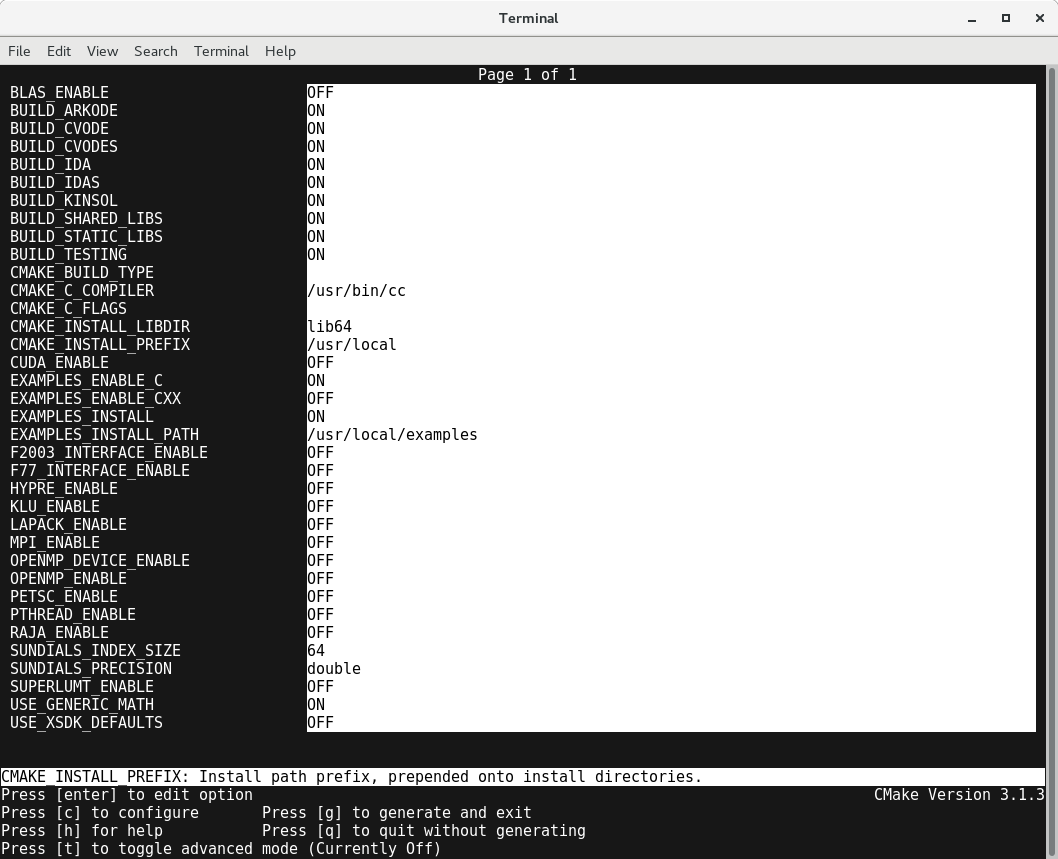
\includegraphics[width=\textwidth]{ccmakedefault}}}
\caption [Initial {\em ccmake} configuration screen]
{Default configuration screen. Note: Initial screen is empty.
To get this default configuration, press 'c' repeatedly (accepting default values denoted with asterisk)
until the 'g' option is available.}
\label{f:ccmakedefault}
\end{figure}

The default {\em instdir} for both {\sundials} and corresponding examples
can be changed by setting the \id{CMAKE\_INSTALL\_PREFIX} and
the \id{EXAMPLES\_INSTALL\_PATH} as shown in figure
\ref{f:ccmakeprefix}.
\begin{figure}[!ht]
{\centerline{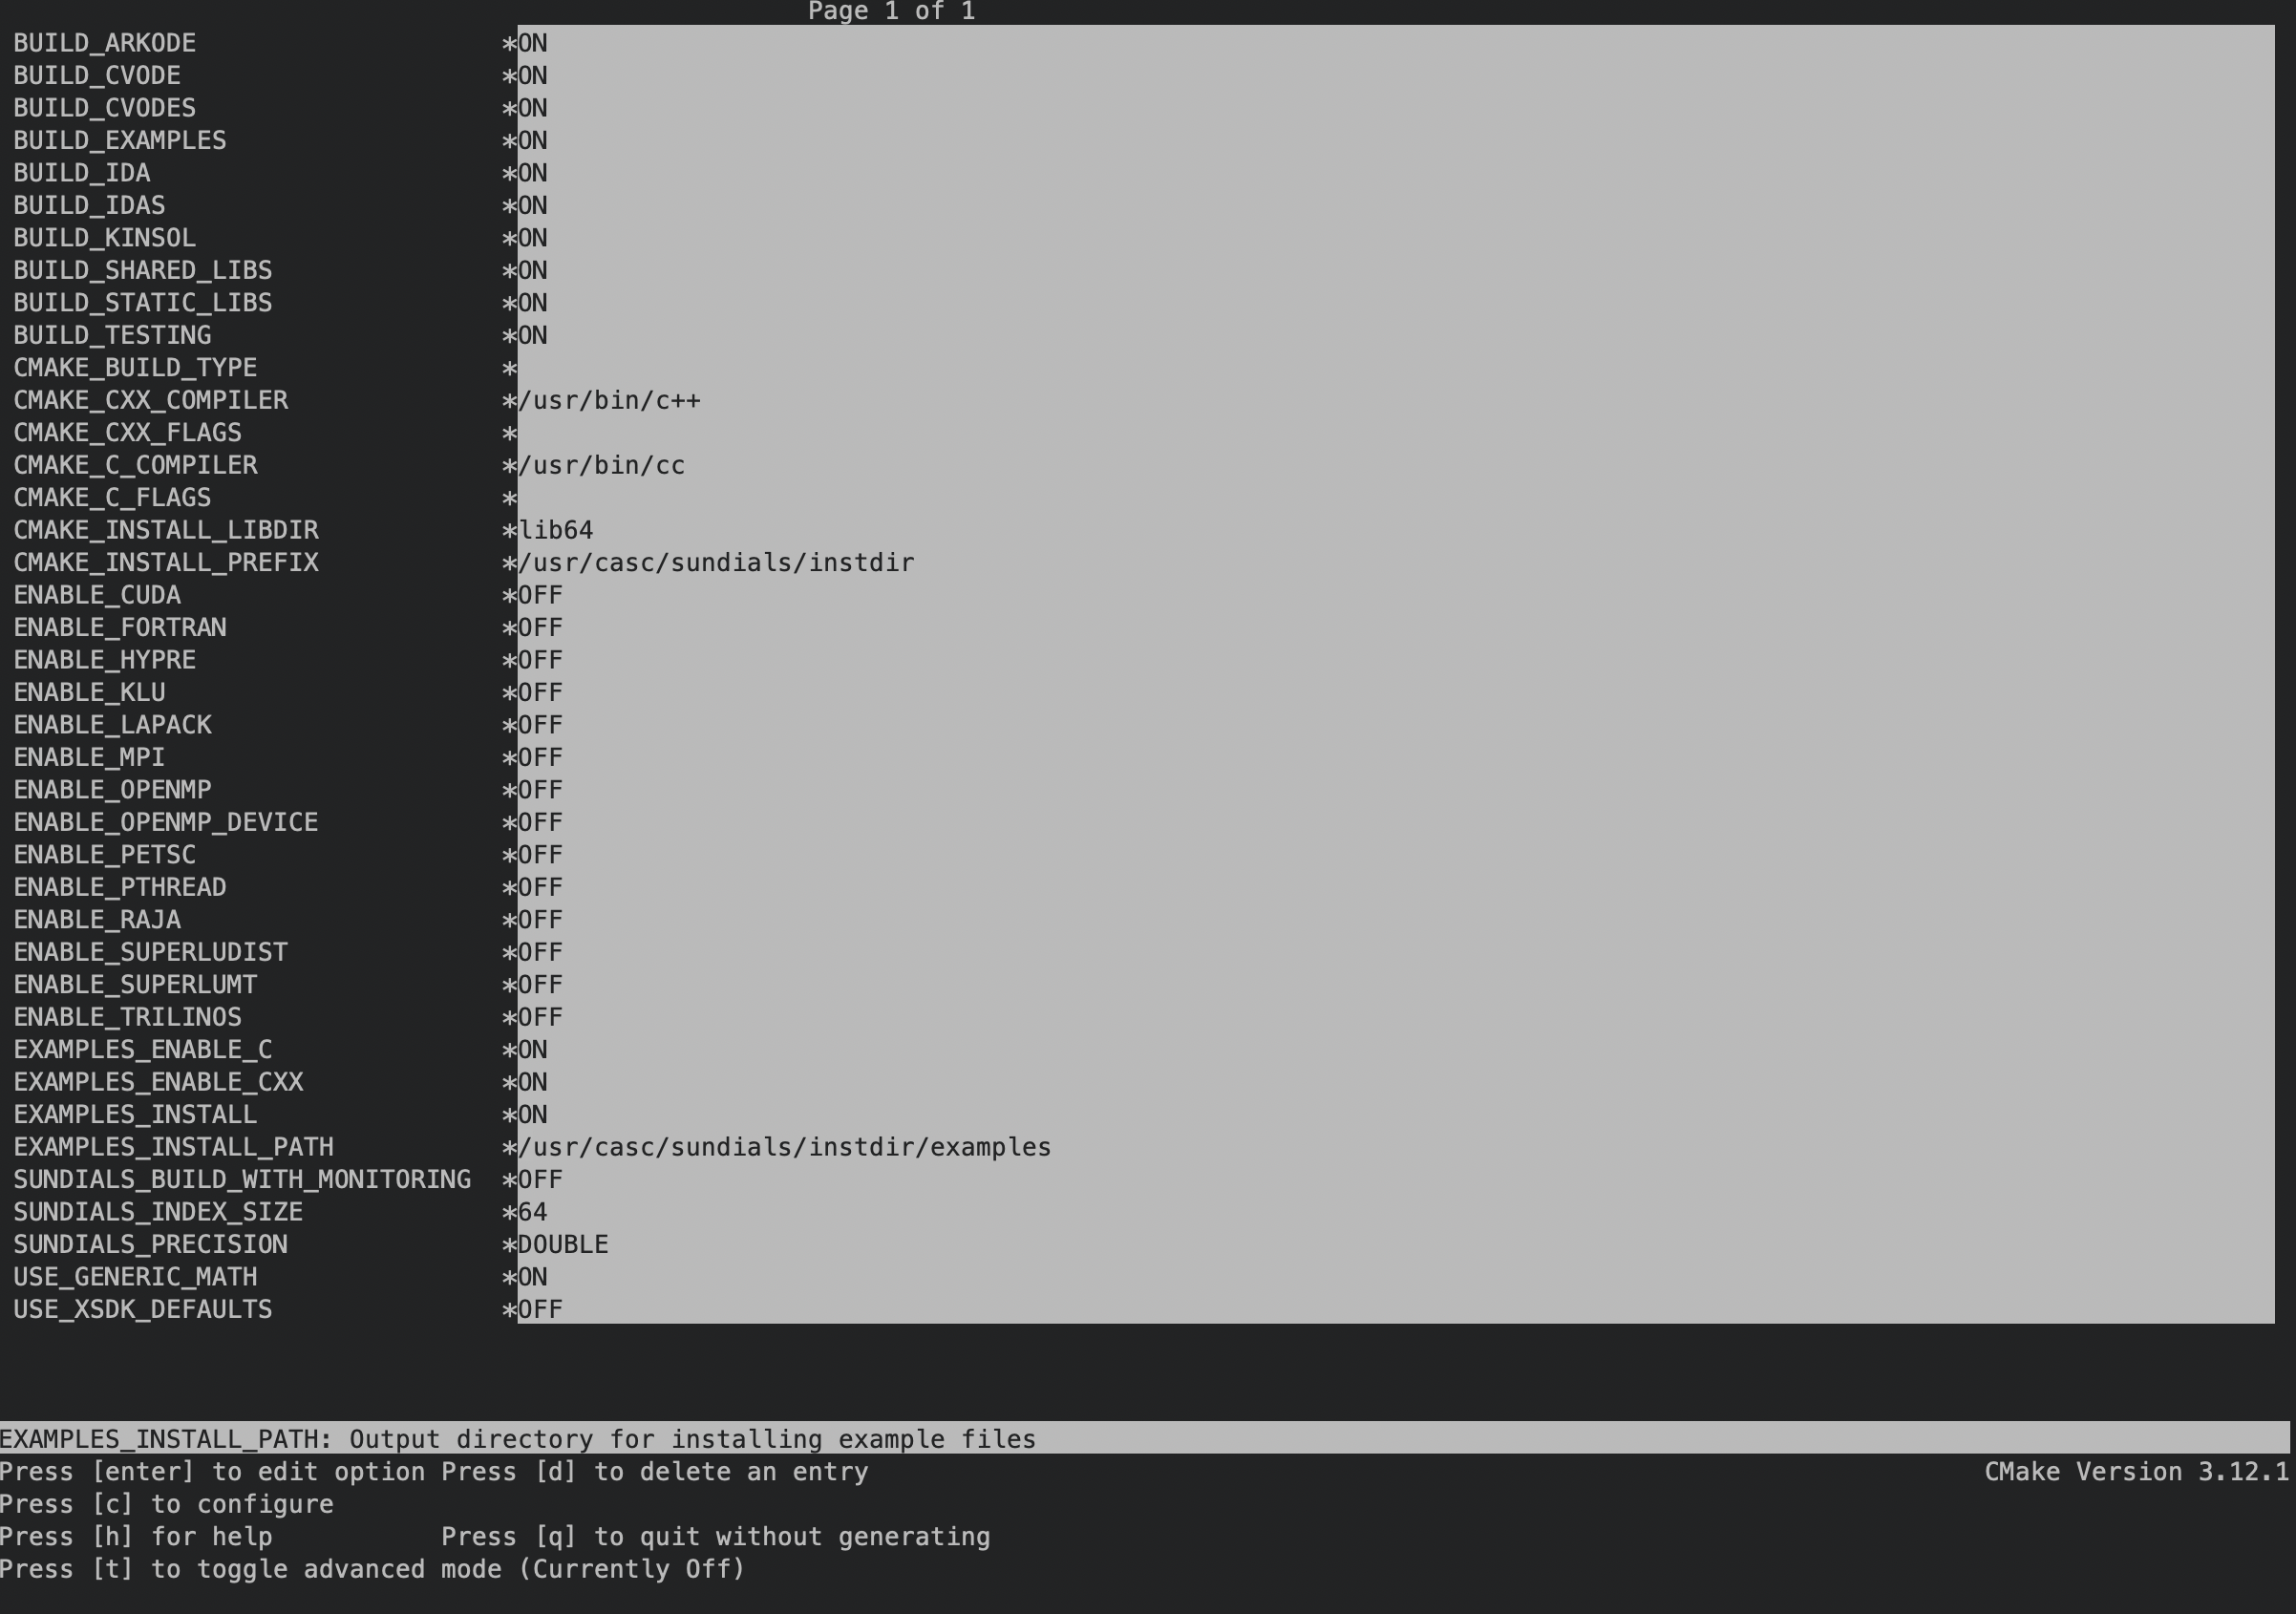
\includegraphics[width=\textwidth]{ccmakeprefix}}}
\caption [Changing the {\em instdir}]
{Changing the {\em instdir} for {\sundials} and
corresponding {\id examples} }
\label{f:ccmakeprefix}
\end{figure}

Pressing the (\id{g} key) will generate makefiles including all dependencies
and all rules to build {\sundials} on this system.
Back at the command prompt, you can now run:

\begin{verbatim}
  % make
\end{verbatim}

To install {\sundials} in the installation directory specified in the configuration, simply run:

\begin{verbatim}
  % make install
\end{verbatim}

%%
%% *** NOTE: The TestRunner will not be distributed at this time.
%% *** Thus the following is commented out from the documentation.
%% TestRunner
%%
%\subsubsection*{Testing Installation}
%The distribution of {\sundials} includes several examples corresponding to the solvers to be
%installed. Also included in the source bundle is a test script: \id{testRunner}, configured by CMake
%to test the included examples.
%To run the tests, enter:

%\begin{verbatim}
%  % make test
%\end{verbatim}
%The output of \id{testRunner} should look similar to the screens in figure
%\ref{f:testrunner}. The success of each test is based on a line-by-line comparison of expected output files, bundled with the source code, with
%the output of the newly compiled examples. The file compare does allow some differences in rounding for float values.\\\\
%NOTE: Some tests may {\em fail} due to differences in machine architecture, compiler versions, third party libraries etc.{\warn}

%\begin{figure}[!ht]
%{\centerline{\includegraphics{figure=testrunnertop.eps,width=\textwidth}}}
%\vspace{3 mm}
%{\centerline{\includegraphics{figure=testrunnerbot.eps,width=\textwidth}}}
%\caption [Running {\em testRunner}]
%{Invoking {\em testRunner} with {\id make test} to execute all configured
%{\id examples} }
%\label{f:testrunner}
%\end{figure}


%%
%% Building from the command line
%%
\subsubsection*{Building from the command line}

Using CMake from the command line is simply a matter of specifying CMake variable settings
with the \id{cmake} command.  The following will build the default configuration:

\begin{verbatim}
   % cmake -DCMAKE_INSTALL_PREFIX=/home/myname/sundials/instdir \
   > -DEXAMPLES_INSTALL_PATH=/home/myname/sundials/instdir/examples \
   > ../solverdir
   % make
   % make install
\end{verbatim}


\subsection{Configuration options (Unix/Linux)}\label{ss:configuration_options_nix}

A complete list of all available options for a CMake-based {\sundials}
configuration is provide below. Note that the default values shown are for
a typical configuration on a Linux system and are provided as illustration only.

\begin{description}
\item[\id{BUILD\_ARKODE}] -
  Build the ARKODE library
  \\
  Default: ON
\item[\id{BUILD\_CVODE}] -
  Build the CVODE library
  \\
  Default: ON
\item[\id{BUILD\_CVODES}] -
  Build the CVODES library
  \\
  Default: ON
\item[\id{BUILD\_IDA}] -
   Build the IDA library
  \\
   Default: ON
\item[\id{BUILD\_IDAS}] -
  Build the IDAS library
  \\
  Default: ON
\item[\id{BUILD\_KINSOL}] -
  Build the KINSOL library
  \\
  Default: ON
\item[\id{BUILD\_SHARED\_LIBS}] -
  Build shared libraries
  \\
  Default: ON
\item[\id{BUILD\_STATIC\_LIBS}] -
  Build static libraries
  \\
  Default: ON
\item[\id{CMAKE\_BUILD\_TYPE}] -
  Choose the type of build, options are:
  \id{None} (CMAKE\_C\_FLAGS used), \id{Debug}, \id{Release},
  \id{RelWithDebInfo}, and \id{MinSizeRel}
  \\
  Default:
  \\
  Note: Specifying a build type will trigger the corresponding
  build type specific compiler flag options below which will be
  appended to the flags set by
  CMAKE\_{\textless}language{\textgreater}\_FLAGS.
\item[\id{CMAKE\_C\_COMPILER}] -
  C compiler
  \\
  Default: /usr/bin/cc
\item[\id{CMAKE\_C\_FLAGS}] -
  Flags for C compiler
  \\
  Default:
\item[\id{CMAKE\_C\_FLAGS\_DEBUG}] -
  Flags used by the C compiler during debug builds
  \\
  Default: -g
\item[\id{CMAKE\_C\_FLAGS\_MINSIZEREL}] -
  Flags used by the C compiler during release minsize builds
  \\
  Default: -Os -DNDEBUG
\item[\id{CMAKE\_C\_FLAGS\_RELEASE}] -
  Flags used by the C compiler during release builds
  \\
  Default: -O3 -DNDEBUG
\item[\id{CMAKE\_CXX\_COMPILER}] -
  {\CPP} compiler
  \\
  Default: /usr/bin/c++
  \\
  Note: A {\CPP} compiler (and all related options) are only
  triggered if {\CPP} examples are enabled (\id{EXAMPLES\_ENABLE\_CXX}
  is ON). All {\sundials} solvers can be used from {\CPP} applications
  by default without setting any additional configuration options.
\item[\id{CMAKE\_CXX\_FLAGS}] -
  Flags for {\CPP} compiler
  \\
  Default:
\item[\id{CMAKE\_CXX\_FLAGS\_DEBUG}] -
  Flags used by the {\CPP} compiler during debug builds
  \\
  Default: -g
\item[\id{CMAKE\_CXX\_FLAGS\_MINSIZEREL}] -
  Flags used by the {\CPP} compiler during release minsize builds
  \\
  Default: -Os -DNDEBUG
\item[\id{CMAKE\_CXX\_FLAGS\_RELEASE}] -
  Flags used by the {\CPP} compiler during release builds
  \\
  Default: -O3 -DNDEBUG
\item[\id{CMAKE\_Fortran\_COMPILER}] -
  Fortran compiler
  \\
  Default: /usr/bin/gfortran
  \\
  Note: Fortran support (and all related options) are triggered only if
  either Fortran-C support is enabled (\id{FCMIX\_ENABLE} is ON) or
  LAPACK support is enabled (\id{LAPACK\_ENABLE} is ON).
\item[\id{CMAKE\_Fortran\_FLAGS}] -
  Flags for Fortran compiler
  \\
  Default:
\item[\id{CMAKE\_Fortran\_FLAGS\_DEBUG}] -
  Flags used by the Fortran compiler during debug builds
  \\
  Default: -g
\item[\id{CMAKE\_Fortran\_FLAGS\_MINSIZEREL}] -
  Flags used by the Fortran compiler during release minsize builds
  \\
  Default: -Os
\item[\id{CMAKE\_Fortran\_FLAGS\_RELEASE}] -
  Flags used by the Fortran compiler during release builds
  \\
  Default: -O3
\item[\id{CMAKE\_INSTALL\_PREFIX}] -
  Install path prefix, prepended onto install directories
  \\
  Default: /usr/local
  \\
  Note: The user must have write access to the location specified through
  this option. Exported {\sundials} header files and libraries will be
  installed under subdirectories \id{include} and
  \id{CMAKE\_INSTALL\_LIBDIR} of \id{CMAKE\_INSTALL\_PREFIX}, respectively.
\item[\id{CMAKE\_INSTALL\_LIBDIR}] -
  Library installation directory
  \\
  Default:
  \\
  Note: This is the directory within \id{CMAKE\_INSTALL\_PREFIX} that the {\sundials}
  libraries will be installed under. The default is automatically set based on the
  operating system using the GNUInstallDirs CMake module.
\item[\id{Fortran\_INSTALL\_MODDIR}] -
  Fortran module installation directory
  \\
  Default: fortran
\item[\id{CUDA\_ENABLE}] -
  Build the {\sundials} {\cuda} modules.
  \\
  Default: OFF
\item[\id{CUDA\_ARCH}] -
  Specifies the CUDA architecture to compile for.
  \\
  Default: sm\_30
\item[\id{EXAMPLES\_ENABLE\_C}] -
  Build the {\sundials} {\CC} examples
  \\
  Default: ON
\item[\id{EXAMPLES\_ENABLE\_CUDA}] -
  Build the {\sundials} {\cuda} examples
  \\
  Default: OFF
  \\
  Note: You need to enable {\cuda} support to build these examples.
\item[\id{EXAMPLES\_ENABLE\_CXX}] -
  Build the {\sundials} {\CPP} examples
  \\
  Default: OFF unless \id{Trilinos\_ENABLE} is ON.
\item[\id{EXAMPLES\_ENABLE\_F77}] -
  Build the {\sundials} Fortran77 examples
  \\
  Default: ON (if \id{F77\_INTERFACE\_ENABLE} is ON)
\item[\id{EXAMPLES\_ENABLE\_F90}] -
  Build the {\sundials} Fortran90 examples
  \\
  Default: ON (if \id{F77\_INTERFACE\_ENABLE} is ON)
\item[\id{EXAMPLES\_ENABLE\_F2003}] -
  Build the {\sundials} Fortran2003 examples
  \\
  Default: ON (if \id{F2003\_INTERFACE\_ENABLE} is ON)
\item[\id{EXAMPLES\_INSTALL}] -
  Install example files
  \\
  Default: ON
  \\
  Note: This option is triggered when any of the {\sundials}
  example programs are enabled \\
  (\id{EXAMPLES\_ENABLE\_$<$language$>$} is ON). If the user requires
  installation of example programs then the sources and sample output files
  for all {\sundials} modules that are currently enabled will be exported to
  the directory specified by \id{EXAMPLES\_INSTALL\_PATH}. A CMake configuration
  script will also be automatically generated and exported to the same directory.
  Additionally, if the configuration is done under a Unix-like system, makefiles
  for the compilation of the example programs (using the installed {\sundials} libraries)
  will be automatically generated and exported to the directory
  specified by \id{EXAMPLES\_INSTALL\_PATH}.
\item[\id{EXAMPLES\_INSTALL\_PATH}] -
  Output directory for installing example files
  \\
  Default: /usr/local/examples
  \\
  Note: The actual default value for this option will be an \id{examples}
  subdirectory created under \id{CMAKE\_INSTALL\_PREFIX}.
\item[\id{F77\_INTERFACE\_ENABLE}] -
  Enable Fortran-C support via the Fortran 77 interfaces
  \\
  Default: OFF
\item[\id{F2003\_INTERFACE\_ENABLE}] -
  Enable Fortran-C support via the Fortran 2003 interfaces
  \\
  Default: OFF
\item[\id{HYPRE\_ENABLE}] -
  Enable {\hypre} support
  \\
  Default: OFF
  \\
  Note: See additional information on building with {\hypre} enabled in
  \ref{ss:externallibs}.
\item[\id{HYPRE\_INCLUDE\_DIR}] -
  Path to {\hypre} header files
\item[\id{HYPRE\_LIBRARY\_DIR}] -
  Path to {\hypre} installed library files
\item[\id{KLU\_ENABLE}] -
  Enable KLU support
  \\
  Default: OFF
  \\
  Note: See additional information on building with KLU enabled in
  \ref{ss:externallibs}.
\item[\id{KLU\_INCLUDE\_DIR}] -
  Path to SuiteSparse header files
\item[\id{KLU\_LIBRARY\_DIR}] -
  Path to SuiteSparse installed library files
\item[\id{LAPACK\_ENABLE}] -
  Enable LAPACK support
  \\
  Default: OFF
  \\
  Note: Setting this option to ON will trigger additional CMake
  options. See additional information on building with LAPACK enabled
  in \ref{ss:externallibs}.
\item[\id{LAPACK\_LIBRARIES}] -
  LAPACK (and BLAS) libraries
  \\
  Default: /usr/lib/liblapack.so;/usr/lib/libblas.so
  \\
  Note: CMake will search for libraries in your \id{LD\_LIBRARY\_PATH} prior
  to searching default system paths.
\item[\id{MPI\_ENABLE}] -
  Enable MPI support. This will build the parallel {\nvector} and the
  MPI-aware version of the ManyVector library.
  \\
  Default: OFF
  \\
  Note: Setting this option to ON will trigger several additional options
  related to MPI.
\item[\id{MPI\_C\_COMPILER}] -
  \id{mpicc} program
  \\
  Default:
\item[\id{MPI\_CXX\_COMPILER}] -
  \id{mpicxx} program
  \\
  Default:
  \\
  Note: This option is triggered only if MPI is enabled
  (\id{MPI\_ENABLE} is ON) and {\CPP} examples are enabled
  (\id{EXAMPLES\_ENABLE\_CXX} is ON). All {\sundials}
  solvers can be used from {\CPP} MPI applications by default
  without setting any additional configuration options other than
  \id{MPI\_ENABLE}.
\item[\id{MPI\_Fortran\_COMPILER}] -
  \id{mpif77} or \id{mpif90} program
  \\
  Default:
  \\
  Note: This option is triggered only if MPI is enabled
  (\id{MPI\_ENABLE} is ON) and Fortran-C support is enabled
  (\id{F77\_INTERFACE\_ENABLE} or \id{F2003\_INTERFACE\_ENABLE} is ON).
\item[\id{MPIEXEC\_EXECUTABLE}] -
  Specify the executable for running MPI programs
  \\
  Default: \id{mpirun}
  \\
  Note: This option is triggered only if MPI is enabled
  (\id{MPI\_ENABLE} is ON).
  %% \\
  %% Note: This can either be set to \id{mpirun} for OpenMPI or \id{srun} if jobs are
  %% managed by \id{SLURM} - Simple Linux Utility for Resource Management as exists on
  %% LLNL's high performance computing clusters.
\item[\id{OPENMP\_ENABLE}] -
  Enable {\openmp} support (build the {\openmp} {\nvector}).
  \\
  Default: OFF
\item[\id{OPENMP\_DEVICE\_ENABLE}] -
  Enable {\openmp} device offloading (build the OpenMPDEV nvector) if supported by
  the provided compiler.
  \\
  Default: OFF
\item[\id{SKIP\_OPENMP\_DEVICE\_CHECK}] - \textbf{advanced option} -
  Skip the check done to see if the {\openmp} provided by the compiler
  supports {\openmp} device offloading.
  \\
  Default: OFF
\item[\id{PETSC\_ENABLE}] -
  Enable {\petsc} support
  \\
  Default: OFF
  \\
  Note: See additional information on building with {\petsc} enabled
  in \ref{ss:build_with_petsc}.
\item[\id{PETSC\_DIR}] -
  Path to {\petsc} installation
  \\
  Default:
\item[\id{PETSC\_LIBRARIES}] - \textbf{advanced option} -
  Semi-colon separated list of PETSc link libraries. Unless provided by the
  user, this is autopopulated based on the PETSc installation found in
  \id{PETSC\_DIR}.
  \\
  Default:
\item[\id{PETSC\_INCLUDES}] - \textbf{advanced option} -
  Semi-colon separated list of PETSc include directories. Unless provided by the
  user, this is autopopulated based on the PETSc installation found in
  \id{PETSC\_DIR}.
  \\
  Default:
\item[\id{PTHREAD\_ENABLE}] -
  Enable Pthreads support (build the Pthreads {\nvector}).
  \\
  Default: OFF
\item[\id{RAJA\_ENABLE}] -
  Enable {\raja} support (build the {\raja} {\nvector}).
  \\
  Default: OFF
  \\
  Note: You need to enable {\cuda} in order to build the {\raja} vector module.
\item[\id{SUNDIALS\_F77\_FUNC\_CASE}] - \textbf{advanced option} -
  Specify the case to use in the Fortran name-mangling scheme, options
  are: \id{lower} or \id{upper}
  \\
  Default:
  \\
  Note: The build system will attempt to infer the Fortran
  name-mangling scheme using the Fortran compiler. This option should
  only be used if a Fortran compiler is not available or to override
  the inferred or default (\id{lower}) scheme if one can not be
  determined. If used, \id{SUNDIALS\_F77\_FUNC\_UNDERSCORES} must also
  be set.
\item[\id{SUNDIALS\_F77\_FUNC\_UNDERSCORES}] - \textbf{advanced option} -
  Specify the number of underscores to append in the Fortran
  name-mangling scheme, options are: \id{none}, \id{one}, or \id{two}
  \\
  Default:
  \\
  Note: The build system will attempt to infer the Fortran
  name-mangling scheme using the Fortran compiler. This option should
  only be used if a Fortran compiler is not available or to override
  the inferred or default (\id{one}) scheme if one can not be
  determined. If used, \id{SUNDIALS\_F77\_FUNC\_CASE} must also be set.
\item[\id{SUNDIALS\_INDEX\_TYPE}] - \textbf{advanced option} -
  Integer type used for {\sundials} indices. The size must match the size provided for
  the \\ \noindent \id{SUNDIALS\_INDEX\_SIZE} option.
  \\
  Default:
  \\
  Note:
  In past SUNDIALS versions, a user could set this option to \id{INT64\_T} to use 64-bit
  integers, or \id{INT32\_T} to use 32-bit integers. Starting in SUNDIALS 3.2.0, these
  special values are deprecated. For SUNDIALS 3.2.0 and up, a user will only need to use
  the \id{SUNDIALS\_INDEX\_SIZE} option in most cases.
\item[\id{SUNDIALS\_INDEX\_SIZE}] -
  Integer size (in bits) used for indices in {\sundials}, options are: \id{32} or \id{64}
  \\
  Default: \id{64}
  \\
  Note:
  The build system tries to find an integer type of appropriate size. Candidate 64-bit
  integer types are (in order of preference): \id{int64\_t}, \id{\_\_int64}, \id{long long}, and \id{long}.
  Candidate 32-bit integers are (in order of preference): \id{int32\_t}, \id{int}, and \id{long}.
  The advanced option, \id{SUNDIALS\_INDEX\_TYPE} can be used to provide a type not listed here.
\item[\id{SUNDIALS\_PRECISION}] -
  Precision used in {\sundials}, options are: \id{double}, \id{single}, or \id{extended}
  \\
  Default: \id{double}
\item[\id{SUPERLUDIST\_ENABLE}] -
  Enable {\superludist} support
  \\
  Default: OFF
  \\
  Note: See additional information on building with {\superludist} enabled
  in \ref{ss:externallibs}.
\item[\id{SUPERLUDIST\_INCLUDE\_DIR}] -
  Path to {\superludist} header files (typically SRC directory)
\item[\id{SUPERLUDIST\_LIBRARY\_DIR}] -
  Path to {\superludist} installed library files
\item[\id{SUPERLUDIST\_LIBRARIES}] -
  Semi-colon separated list of libraries needed for {\superludist}
\item[\id{SUPERLUDIST\_OpenMP}] -
  Enable {\sundials} support for {\superludist} built with {\openmp}
  \\
  Default: OFF
  \\
  Note: {\superludist} must be built with {\openmp} support for this option to function
  properly. Additionally the environment variable \id{OMP\_NUM\_THREADS} must be set to
  the desired number of threads.
\item[\id{SUPERLUMT\_ENABLE}] -
  Enable {\superlumt} support
  \\
  Default: OFF
  \\
  Note: See additional information on building with {\superlumt} enabled
  in \ref{ss:externallibs}.
\item[\id{SUPERLUMT\_INCLUDE\_DIR}] -
  Path to SuperLU\_MT header files (typically SRC directory)
\item[\id{SUPERLUMT\_LIBRARY\_DIR}] -
  Path to SuperLU\_MT installed library files
\item[\id{SUPERLUMT\_LIBRARIES}] -
  Semi-colon separated list of libraries needed for SuperLU\_MT
\item[\id{SUPERLUMT\_THREAD\_TYPE}] -
  Must be set to Pthread or {\openmp}
  \\
  Default: Pthread
\item[\id{Trilinos\_ENABLE}] -
  Enable {\trilinos} support (build the {\tpetra} {\nvector}).
  \\
  Default: OFF
\item[\id{Trilinos\_DIR}] -
  Path to the Trilinos install directory.
  \\
  Default:
\item[\id{TRILINOS\_INTERFACE\_C\_COMPILER}] - \textbf{advanced option} -
  Set the {\CC} compiler for building the {\trilinos} interface
  (i.e., {\nvectrilinos} and the examples that use it).
  \\
  Default: The {\CC} compiler exported from the found {\trilinos} installation
  if \id{USE\_XSDK\_DEFAULTS=OFF}. \id{CMAKE\_C\_COMPILER} or \id{MPI\_C\_COMPILER} if \id{USE\_XSDK\_DEFAULTS=ON}.
  \\
  Note: It is recommended to use the same compiler that was used to build the {\trilinos} library.
\item[\id{TRILINOS\_INTERFACE\_C\_COMPILER\_FLAGS}] - \textbf{advanced option} -
  Set the {\CC} compiler flags for {\trilinos} interface
  (i.e., {\nvectrilinos} and the examples that use it).
  \\
  Default: The {\CC} compiler flags exported from the found {\trilinos} installation
  if \id{USE\_XSDK\_DEFAULTS=OFF}. \id{CMAKE\_C\_FLAGS} if \id{USE\_XSDK\_DEFAULTS=ON}.
  \\
  Note: It is recommended to use the same flags that were used to build the {\trilinos} library.
\item[\id{TRILINOS\_INTERFACE\_CXX\_COMPILER}] - \textbf{advanced option} -
  Set the {\CPP} compiler for builing {\trilinos} interface
  (i.e., {\nvectrilinos} and the examples that use it).
  \\
  Default: The {\CPP} compiler exported from the found {\trilinos} installation
  if \id{USE\_XSDK\_DEFAULTS=OFF}. \id{CMAKE\_CXX\_COMPILER} or \id{MPI\_CXX\_COMPILER} if \id{USE\_XSDK\_DEFAULTS=ON}.
  \\
  Note: It is recommended to use the same compiler that was used to build the {\trilinos} library.
\item[\id{TRILINOS\_INTERFACE\_CXX\_COMPILER\_FLAGS}] - \textbf{advanced option} -
  Set the {\CPP} compiler flags for {\trilinos} interface
  (i.e., {\nvectrilinos} and the examples that use it).
  \\
  Default: The {\CPP} compiler flags exported from the found {\trilinos} installation
  if \id{USE\_XSDK\_DEFAULTS=OFF}. \id{CMAKE\_CXX\_FLAGS} if \id{USE\_XSDK\_DEFAULTS=ON}.
  \\
  Note: Is is recommended to use the same flags that were used to build the {\trilinos} library.
\item[\id{USE\_GENERIC\_MATH}] -
  Use generic (stdc) math libraries
  \\
  Default: ON



\end{description}

\subsubsection*{xSDK Configuration Options}

{\sundials} supports CMake configuration options defined by the
Extreme-scale Scientific Software Development Kit (xSDK) community
policies (see {\tt https://xsdk.info} for more information). xSDK
CMake options are unused by default but may be activated by setting
\id{USE\_XSDK\_DEFAULTS} to ON.

{\warn} When xSDK options are active, they will overwrite the
corresponding {\sundials} option and may have different default values
(see details below). As such the equivalent {\sundials} options should
not be used when configuring with xSDK options. In the GUI front end
to CMake (\id{ccmake}), setting \id{USE\_XSDK\_DEFAULTS} to ON will
hide the corresponding {\sundials} options as advanced CMake variables.
During configuration, messages are output detailing
which xSDK flags are active and the equivalent {\sundials} options
that are replaced. Below is a complete list xSDK options and the
corresponding {\sundials} options if applicable.

\begin{description}
\item[\id{TPL\_ENABLE\_HYPRE}] -
  Enable {\hypre} support
  \\
  Default: OFF
  \\
  {\sundials} equivalent: \id{HYPRE\_ENABLE}
\item[\id{TPL\_ENABLE\_KLU}] -
  Enable KLU support
  \\
  Default: OFF
  \\
  {\sundials} equivalent: \id{KLU\_ENABLE}
\item[\id{TPL\_ENABLE\_PETSC}] -
  Enable {\petsc} support
  \\
  Default: OFF
  \\
  {\sundials} equivalent: \id{PETSC\_ENABLE}
\item[\id{TPL\_ENABLE\_LAPACK}] -
  Enable LAPACK support
  \\
  Default: OFF
  \\
  {\sundials} equivalent: \id{LAPACK\_ENABLE}
\item[\id{TPL\_ENABLE\_SUPERLUDIST}] -
  Enable {\superludist} support
  \\
  Default: OFF
  \\
  {\sundials} equivalent: \id{SUPERLUDIST\_ENABLE}
\item[\id{TPL\_ENABLE\_SUPERLUMT}] -
  Enable SuperLU\_MT support
  \\
  Default: OFF
  \\
  {\sundials} equivalent: \id{SUPERLUMT\_ENABLE}
\item[\id{TPL\_HYPRE\_INCLUDE\_DIRS}] -
  Path to {\hypre} header files
  \\
  {\sundials} equivalent: \id{HYPRE\_INCLUDE\_DIR}
\item[\id{TPL\_HYPRE\_LIBRARIES}] -
  {\hypre} library
  \\
  {\sundials} equivalent: N/A
\item[\id{TPL\_KLU\_INCLUDE\_DIRS}] -
  Path to KLU header files
  \\
  {\sundials} equivalent: \id{KLU\_INCLUDE\_DIR}
\item[\id{TPL\_KLU\_LIBRARIES}] -
  KLU library
  \\
  {\sundials} equivalent: N/A
\item[\id{TPL\_LAPACK\_LIBRARIES}] -
  LAPACK (and BLAS) libraries
  \\
  Default: /usr/lib/liblapack.so;/usr/lib/libblas.so
  \\
  {\sundials} equivalent: \id{LAPACK\_LIBRARIES}
  \\
  Note: CMake will search for libraries in your \id{LD\_LIBRARY\_PATH} prior
  to searching default system paths.
\item[\id{TPL\_PETSC\_DIR}] -
  Path to {\petsc} installation
  \\
  {\sundials} equivalent: \id{PETSC\_DIR}
\item[\id{TPL\_SUPERLUDIST\_INCLUDE\_DIRS}] -
  Path to {\superludist} header files
  \\
  {\sundials} equivalent: \id{SUPERLUDIST\_INCLUDE\_DIR}
\item[\id{TPL\_SUPERLUDIST\_LIBRARIES}] -
  Semi-colon separated list of libraries needed for {\superludist}
  including the {\superludist} library itself
  \\
  {\sundials} equivalent: \id{SUPERLUDIST\_LIBRARIES}
\item[\id{TPL\_SUPERLUDIST\_OPENMP}] -
  Enable {\sundials} support for {\superludist} built with {\openmp}
  \\
  {\sundials} equivalent: \id{SUPERLUDIST\_OPENMP}
\item[\id{TPL\_SUPERLUMT\_LIBRARIES}] -
  SuperLU\_MT library
  \\
  {\sundials} equivalent: N/A
\item[\id{TPL\_SUPERLUMT\_THREAD\_TYPE}] -
  SuperLU\_MT library thread type
  \\
  {\sundials} equivalent: \id{SUPERLUMT\_THREAD\_TYPE}
\item[\id{USE\_XSDK\_DEFAULTS}] -
  Enable xSDK default configuration settings
  \\
  Default: OFF
  \\
  {\sundials} equivalent: N/A
  \\
  Note: Enabling xSDK defaults also sets \id{CMAKE\_BUILD\_TYPE} to \id{Debug}
\item[\id{XSDK\_ENABLE\_FORTRAN}] -
  Enable {\sundials} Fortran interfaces
  \\
  Default: OFF
  \\
  {\sundials} equivalent: \id{F77\_INTERFACE\_ENABLE}/\id{F2003\_INTERFACE\_ENABLE}
\item[\id{XSDK\_INDEX\_SIZE}] -
  Integer size (bits) used for indices in {\sundials}, options are: \id{32} or \id{64}
  \\
  Default: \id{32}
  \\
  {\sundials} equivalent: \id{SUNDIALS\_INDEX\_SIZE}
\item[\id{XSDK\_PRECISION}] -
  Precision used in {\sundials}, options are: \id{double}, \id{single}, or \id{quad}
  \\
  Default: \id{double}
  \\
  {\sundials} equivalent: \id{SUNDIALS\_PRECISION}
\end{description}



%%===============================================================================

\subsection{Configuration examples}

The following examples will help demonstrate usage of the CMake configure options.

\noindent To configure {\sundials} using the default C and Fortran compilers,
and default \id{mpicc} and \id{mpif77} parallel compilers,
enable compilation of examples, and install libraries, headers, and
example sources under subdirectories of
\id{/home/myname/sundials/}, use:

\begin{verbatim}
   % cmake \
   > -DCMAKE_INSTALL_PREFIX=/home/myname/sundials/instdir \
   > -DEXAMPLES_INSTALL_PATH=/home/myname/sundials/instdir/examples \
   > -DMPI_ENABLE=ON \
   > -DFCMIX_ENABLE=ON \
   > /home/myname/sundials/solverdir
   %
   % make install
   %
\end{verbatim}

\noindent To disable installation of the examples, use:
\begin{verbatim}
   % cmake \
   > -DCMAKE_INSTALL_PREFIX=/home/myname/sundials/instdir \
   > -DEXAMPLES_INSTALL_PATH=/home/myname/sundials/instdir/examples \
   > -DMPI_ENABLE=ON \
   > -DFCMIX_ENABLE=ON \
   > -DEXAMPLES_INSTALL=OFF \
   > /home/myname/sundials/solverdir
   %
   % make install
   %
\end{verbatim}

%%===============================================================================
\subsection{Working with external Libraries} \label{ss:externallibs}

The {\sundials} suite contains many options to enable implementation flexibility
when developing solutions. The following are some notes addressing specific configurations
when using the supported third party libraries.
When building {\sundials} as a shared library any external libraries
used with {\sundials} must also be build as a shared library or as a
static library compiled with the \id{-fPIC} flag.{\warn}

\subsubsection*{Building with LAPACK}
To enable LAPACK, set the \id{LAPACK\_ENABLE} option to \id{ON}.
If the directory containing the LAPACK library is in the
\id{LD\_LIBRARY\_PATH} environment variable, CMake will set the
\id{LAPACK\_LIBRARIES} variable accordingly, otherwise CMake will
attempt to find the LAPACK library in standard system locations. To
explicitly tell CMake what library to use, the \id{LAPACK\_LIBRARIES}
variable can be set to the desired libraries rquired for LAPACK.
\begin{verbatim}
   % cmake \
   > -DCMAKE_INSTALL_PREFIX=/home/myname/sundials/instdir \
   > -DEXAMPLES_INSTALL_PATH=/home/myname/sundials/instdir/examples \
   > -DLAPACK_ENABLE=ON \
   > -DLAPACK_LIBRARIES=/mylapackpath/lib/libblas.so;/mylapackpath/lib/liblapack.so \
   > /home/myname/sundials/solverdir
   %
   % make install
   %
\end{verbatim}

If a working Fortran compiler is not available to infer the Fortran
name-mangling scheme, the options \id{SUNDIALS\_F77\_FUNC\_CASE} and
\id{SUNDIALS\_F77\_FUNC\_UNDERSCORES} \textit{must} be set in order to
bypass the check for a Fortran compiler and define the name-mangling
scheme. The defaults for these options in earlier versions of
{\sundials} were \id{lower} and \id{one} respectively.

\subsubsection*{Building with KLU}
The KLU libraries are part of SuiteSparse, a suite of sparse matrix software,
available from the Texas A\&M University website: {\tt
http://faculty.cse.tamu.edu/davis/suitesparse.html}.  {\sundials} has been
tested with SuiteSparse version 5.3.0.  To enable KLU, set \id{KLU\_ENABLE} to
\id{ON}, set \id{KLU\_INCLUDE\_DIR} to the \id{include} path of the KLU
installation and set \id{KLU\_LIBRARY\_DIR} to the \id{lib} path of the KLU
installation.  The CMake configure will result in populating the following
variables: \id{AMD\_LIBRARY}, \id{AMD\_LIBRARY\_DIR}, \id{BTF\_LIBRARY},
\id{BTF\_LIBRARY\_DIR}, \id{COLAMD\_LIBRARY}, \id{COLAMD\_LIBRARY\_DIR}, and
\newline\id{KLU\_LIBRARY}.

\subsubsection*{Building with SuperLU\_MT}
The SuperLU\_MT libraries are available for download from the Lawrence Berkeley
National Laboratory website: {\tt
http://crd-legacy.lbl.gov/$\sim$xiaoye/SuperLU/\#superlu\_mt}.  {\sundials} has
been tested with SuperLU\_MT version 3.1.  To enable SuperLU\_MT, set
\id{SUPERLUMT\_ENABLE} to \id{ON}, set \id{SUPERLUMT\_INCLUDE\_DIR} to the
\id{SRC} path of the SuperLU\_MT installation, and set the variable
\newline\id{SUPERLUMT\_LIBRARY\_DIR} to the \id{lib} path of the SuperLU\_MT
installation.  At the same time, the variable \id{SUPERLUMT\_LIBRARIES} must be
set to a semi-colon separated list of other libraries SuperLU\_MT depends on.
For example, if SuperLU\_MT ws build with an external blas library, then include
the full path to the blas library in this list. Additionally, the variable
\id{SUPERLUMT\_THREAD\_TYPE} must be set to either \id{Pthread} or
\id{{\openmp}}.

\noindent Do not mix thread types when building {\sundials} solvers.  If
threading is enabled for {\sundials} by having either \id{OPENMP\_ENABLE} or
\id{PTHREAD\_ENABLE} set to \id{ON} then SuperLU\_MT should be set to use the
same threading type.{\warn}

\subsubsection*{Building with {\superludist}}
The {\superludist} libraries are available for download from the Lawrence
Berkeley National Laboratory website: {\tt
http://crd-legacy.lbl.gov/$\sim$xiaoye/SuperLU/\#superlu\_dist}.  {\sundials}
has been tested with {\superludist} 6.1.1.  To enable {\superludist}, set
\id{SUPERLUDIST\_ENABLE} to \id{ON}, set \id{SUPERLUDIST\_INCLUDE\_DIR} to the
include directory of the {\superludist} installation (typically \id{SRC}), and
set the variable \newline\id{SUPERLUDIST\_LIBRARY\_DIR} to the path to library
directory of the {\superludist} installation (typically \id{lib}). At the same
time, the variable \id{SUPERLUDIST\_LIBRARIES} must be set to a semi-colon
separated list of other libraries {\superludist} depends on. For example, if
{\superludist} was built with LAPACK, then include the LAPACK library in this
list.  If {\superludist} was built with {\openmp} support, then you may set
\id{SUPERLUDIST\_OPENMP} to \id{ON} to utilize the {\openmp} functionality of
{\superludist}.

\noindent Do not mix thread types when building {\sundials} solvers.  If
threading is enabled for {\sundials} by having \id{PTHREAD\_ENABLE} set to
\id{ON} then {\superludist} should not be set to use {\openmp}.{\warn}

\subsubsection*{Building with PETSc}
\label{ss:building_with_petsc}
The {\petsc} libraries are available for download from the Argonne National
Laboratory website: {\tt http://www.mcs.anl.gov/petsc}. {\sundials} has been
tested with {\petsc} version 3.10.0--3.12.1. To enable {\petsc}, set
\id{PETSC\_ENABLE} to \id{ON} and then set \id{PETSC\_DIR} to the path of the
{\petsc} installation. Alternatively, a user can provide a list of include paths
in \id{PETSC\_INCLUDES}, and a list of complete paths to the libraries needed in
\id{PETSC\_LIBRARIES}.


\subsubsection*{Building with {\hypre}}
The {\hypre} libraries are available for download from the Lawrence Livermore
National Laboratory website: {\tt http://computing.llnl.gov/projects/hypre}.
{\sundials} has been tested with {\hypre} version 2.14.0--2.18.0.  To enable
{\hypre}, set  \id{HYPRE\_ENABLE} to \id{ON}, set \id{HYPRE\_INCLUDE\_DIR} to
the \id{include} path of the {\hypre} installation, and set the variable
\id{HYPRE\_LIBRARY\_DIR} to the \id{lib} path of the {\hypre} installation.

Note: {\sundials} must be configured so that \id{SUNDIALS\_INDEX\_SIZE} (or
equivalently, \id{XSDK\_INDEX\_SIZE}) equals the precision of
\id{HYPRE\_BigInt} in the corresponding {\hypre} installation.


\subsubsection*{Building with CUDA}
{\sundials} {\cuda} modules and examples have been tested with versions 9
through 10.1 of the {\cuda} toolkit. To build them, you need to install the
Toolkit and compatible NVIDIA drivers. Both are available for download from the
NVIDIA website: {\tt https://developer.nvidia.com/cuda-downloads}. To enable
{\cuda}, set \id{CUDA\_ENABLE} to \id{ON}. If {\cuda} is installed in a
nonstandard location, you may be prompted to set the variable
\id{CUDA\_TOOLKIT\_ROOT\_DIR} with your {\cuda} Toolkit installation path. To
enable {\cuda} examples, set \id{EXAMPLES\_ENABLE\_CUDA} to \id{ON}.

\subsubsection*{Building with RAJA}
{\raja} is a performance portability layer developed by Lawrence Livermore
National Laboratory and can be obtained from {\tt https://github.com/LLNL/RAJA}.
{\sundials} {\raja} modules and examples have been tested with {\raja} up to
version 0.9. Building {\sundials} {\raja} modules requires a {\cuda}-enabled
{\raja} installation. To enable {\raja}, set \id{CUDA\_ENABLE} and
\id{RAJA\_ENABLE} to \id{ON}. If {\raja} is installed in a nonstandard location
you will be prompted to set the variable \id{RAJA\_DIR} with the path to the
{\raja} CMake configuration file. To enable building the {\raja} examples set
\id{EXAMPLES\_ENABLE\_CUDA} to \id{ON}.

\subsubsection*{Building with Trilinos}
{\trilinos} is a suite of numerical libraries developed by Sandia National
Laboratories. It can be obtained at {\tt https://github.com/trilinos/Trilinos}.
{\sundials} {\trilinos} modules and examples have been tested with {\trilinos}
version 12.14.1. To enable {\trilinos}, set
\id{Trilinos\_ENABLE} to \id{ON}. If {\trilinos} is
installed in a nonstandard location you will be prompted to set the
variable \id{Trilinos\_DIR} with the path to the {\trilinos} CMake
configuration file. It is desireable to build the {\trilinos} vector interface
with same compiler and options that were used to build {\trilinos}.
CMake will try to find the correct compiler settings automatically from the
{\trilinos} configuration file. If that is not successful,
the compilers and options can be manually set with the following CMake variables:
\begin{itemize}
\item
\id{Trilinos\_INTERFACE\_C\_COMPILER}
\item
\id{Trilinos\_INTERFACE\_C\_COMPILER\_FLAGS}
\item
\id{Trilinos\_INTERFACE\_CXX\_COMPILER}
\item
\id{Trilinos\_INTERFACE\_CXX\_COMPILER\_FLAGS}
\end{itemize}

\subsection{Testing the build and installation}

If {\sundials} was configured with
\id{EXAMPLES\_ENABLE\_$<$language$>$} options to \id{ON}, then a set of
regression tests can be run after building with the \id{make} command
by running:
\begin{verbatim}
  % make test
\end{verbatim}
Additionally, if \id{EXAMPLES\_INSTALL} was also set to \id{ON}, then
a set of smoke tests can be run after installing with the \id{make install}
command by running:
\begin{verbatim}
  % make test_install
\end{verbatim}

%%===============================================================================
\section{Building and Running Examples}
%%===============================================================================
Each of the {\sundials} solvers is distributed with a set of examples
demonstrating basic usage. To build and install the examples, set at least of
the \id{EXAMPLES\_ENABLE\_$<$language$>$} options to \id{ON}, and set
\id{EXAMPLES\_INSTALL} to \id{ON}.  Specify the installation path for the
examples with the variable \id{EXAMPLES\_INSTALL\_PATH}. CMake will generate
\id{CMakeLists.txt} configuration files (and \id{Makefile} files if on
Linux/Unix) that reference the {\em installed} {\sundials} headers and
libraries.

Either the \id{CMakeLists.txt} file or the traditional \id{Makefile} may be used
to build the examples as well as serve as a template for creating user developed
solutions.  To use the supplied \id{Makefile} simply run \id{make} to compile
and generate the executables.  To use CMake from within the installed example
directory, run \id{cmake} (or \id{ccmake} to use the GUI) followed by \id{make}
to compile the example code.  Note that if CMake is used, it will overwrite the
traditional \id{Makefile} with a new CMake-generated \id{Makefile}.  The
resulting output from running the examples can be compared with example output
bundled in the {\sundials} distribution.

\noindent NOTE: There will potentially be differences in the output due to
machine architecture, compiler versions, use of third party libraries
etc.{\warn}


%%===============================================================================
\section{Configuring, building, and installing  on Windows}\label{s:cmake_windows}
%%===============================================================================
CMake can also be used to build {\sundials} on Windows. To build {\sundials} for
use with Visual Studio the following steps should be performed:
\begin{enumerate}
\item Unzip the downloaded tar file(s) into a directory. This will be the {\em solverdir}
\item Create a separate {\em builddir}
\item Open a Visual Studio Command Prompt and cd to {\em builddir}
\item Run cmake-gui ../{\em solverdir}
\begin{enumerate}
\item Hit Configure
\item Check/Uncheck solvers to be built
\item Change CMAKE\_INSTALL\_PREFIX to {\em instdir}
\item Set other options as desired
\item Hit Generate
\end{enumerate}
\item Back in the VS Command Window:
\begin{enumerate}
\item Run msbuild ALL\_BUILD.vcxproj
\item Run msbuild INSTALL.vcxproj
\end{enumerate}
\end{enumerate}

\noindent The resulting libraries will be in the {\em instdir}.
\noindent The {\sundials} project can also now be opened in Visual Studio.
Double click on the ALL\_BUILD.vcxproj file to open the project.
Build the whole {\em solution} to create the {\sundials} libraries.
To use the {\sundials} libraries in your own projects, you must
set the include directories for your project,
add the {\sundials} libraries to your project solution,
and set the {\sundials} libraries as dependencies for your project.

%%===============================================================================
\section{Installed libraries and exported header files}
%%===============================================================================

Using the CMake {\sundials} build system, the command
\begin{verbatim}
   % make install
\end{verbatim}
will install the libraries under {\em libdir} and the public header
files under {\em includedir}. The values for these directories are
{\em instdir}\id{/CMAKE\_INSTALL\_LIBDIR} and {\em instdir}\id{/include},
respectively. The location can be changed by setting the CMake variable \id{CMAKE\_INSTALL\_PREFIX}.
Although all installed libraries reside under {\em libdir}\id{/CMAKE\_INSTALL\_LIBDIR}, the public
header files are further organized into subdirectories under {\em includedir}\id{/include}.

The installed libraries and exported header files are listed for
reference in Table \ref{t:sundials_files}.
The file extension .{\em lib}
is typically \id{.so} for shared libraries and \id{.a} for static libraries.
Note that, in the Tables, names are relative to {\em libdir}
for libraries and to {\em includedir} for header files.

A typical user program need not explicitly include any of the shared
{\sundials} header files from under the {\em includedir}\id{/include}\id{/sundials}
directory since they are explicitly included by the appropriate solver
header files ({\em e.g.}, \id{cvode\_dense.h} includes
\id{sundials\_dense.h}). However, it is both legal and safe to do so,
and would be useful, for example, if the functions declared in \id{sundials\_dense.h}
are to be used in building a preconditioner.

%---------------------------------------------------------------------------
% Table of installed files
%---------------------------------------------------------------------------

\newlength{\colLenOne}
\settowidth{\colLenOne}{{\sunnonlinsolfixedpoint}}

\newlength{\colLenTwo}
\settowidth{\colLenTwo}{Header files}

\newlength{\colLenThree}
\setlength{\colLenThree}{\textwidth}
\addtolength{\colLenThree}{-0.5in}
\addtolength{\colLenThree}{-\colLenOne}
\addtolength{\colLenThree}{-\colLenTwo}

%\caption{{\sundials} libraries and header files (cont.)}\label{t:sundials_files2}

\clearpage
\tablecaption{{\sundials} libraries and header files}\label{t:sundials_files}
\tablefirsthead{\hline}
\tablehead{\hline \multicolumn{4}{|l|}{\small\slshape continued from last page} \\
           \hline}
\tabletail{\hline \multicolumn{4}{|r|}{\small\slshape continued on next page} \\ \hline}
\begin{xtabular}{|p{\colLenOne}|p{\colLenTwo}|p{0.5\colLenThree} p{0.5\colLenThree}|}

%% --------------------------------------------------
{\shared}
 & Libraries    & n/a  & \\
\cline{2-4}
& Header files & sundials/sundials\_config.h                         &                           \\
&              & sundials/sundials\_fconfig.h                        &                           \\
&              & sundials/sundials\_types.h                          &                           \\
&              & sundials/sundials\_math.h                           &                           \\
&              & sundials/sundials\_nvector.h                        &                           \\
&              & sundials/sundials\_fnvector.h                       &                           \\
&              & sundials/sundials\_matrix.h                         &                           \\
&              & sundials/sundials\_linearsolver.h                   &                           \\
&              & sundials/sundials\_iterative.h                      &                           \\
&              & sundials/sundials\_direct.h                         &                           \\
&              & sundials/sundials\_dense.h                          &                           \\
&              & sundials/sundials\_band.h                           &                           \\
&              & sundials/sundials\_nonlinearsolver.h                &                           \\
&              & sundials/sundials\_version.h                        &                           \\
&              & sundials/sundials\_mpi\_types.h                     &                           \\
\hline
%% --------------------------------------------------
{\nvecs}
& Libraries    & libsundials\_nvecserial.{\em lib}                   &                           \\
&              & libsundials\_fnvecserial\_mod.{\em lib}             &                           \\
&              & libsundials\_fnvecserial.a                          &                           \\
\cline{2-4}
& Header files & nvector/nvector\_serial.h                           &                           \\
\cline{2-4}
& Module files & fnvector\_serial\_mod.mod                           &                           \\
\hline
%% --------------------------------------------------
{\nvecp}
& Libraries    & libsundials\_nvecparallel.{\em lib}                 &                           \\
&              & libsundials\_fnvecparallel.a                        &                           \\
&              & libsundials\_fnvecparallel\_mod.{\em lib}           &                           \\
\cline{2-4}
& Header files & nvector/nvector\_parallel.h                         &                           \\
\cline{2-4}
& Module files & fnvector\_parallel\_mod.mod                         &                           \\
\hline
%% --------------------------------------------------
{\nvecmanyvector}
& Libraries    & libsundials\_nvecmanyvector.{\em lib}               &                           \\
&              & libsundials\_nvecmanyvector\_mod.{\em lib}          &                           \\
\cline{2-4}
& Header files & nvector/nvector\_manyvector.h                       &                           \\
\cline{2-4}
& Module files & fnvector\_manyvector\_mod.mod                       &                           \\
\hline
%% --------------------------------------------------
{\nvecmpimanyvector}
& Libraries    & libsundials\_nvecmpimanyvector.{\em lib}            &                           \\
&              & libsundials\_nvecmpimanyvector\_mod.{\em lib}       &                           \\
\cline{2-4}
& Header files & nvector/nvector\_mpimanyvector.h                    &                           \\
\cline{2-4}
& Module files & fnvector\_mpimanyvector\_mod.mod                    &                           \\
\hline
%% --------------------------------------------------
{\nvecmpiplusx}
& Libraries    & libsundials\_nvecmpiplusx.{\em lib}                 &                           \\
&              & libsundials\_nvecmpiplusx\_mod.{\em lib}            &                           \\
\cline{2-4}
& Header files & nvector/nvector\_mpiplusx.h                         &                           \\
\cline{2-4}
& Module files & fnvector\_mpiplusx\_mod.mod                         &                           \\
\hline
%% --------------------------------------------------
{\nvecopenmp}
& Libraries    & libsundials\_nvecopenmp.{\em lib}                   &                           \\
&              & libsundials\_fnvecopenmp\_mod.{\em lib}             &                           \\
&              & libsundials\_fnvecopenmp.a                          &                           \\
\cline{2-4}
& Header files & nvector/nvector\_openmp.h                           &                           \\
\cline{2-4}
& Module files & fnvector\_openmp\_mod.mod                           &                           \\
\hline
%% --------------------------------------------------
{\nvecopenmpdev}
& Libraries    & libsundials\_nvecopenmpdev.{\em lib}                &                           \\
\cline{2-4}
& Header files & nvector/nvector\_openmpdev.h                        &                           \\
\hline
%% --------------------------------------------------
{\nvecpthreads}
& Libraries    & libsundials\_nvecpthreads.{\em lib}                 &                           \\
&              & libsundials\_fnvecpthreads\_mod.{\em lib}           &                           \\
&              & libsundials\_fnvecpthreads.a                        &                           \\
\cline{2-4}
& Header files & nvector/nvector\_pthreads.h                         &                           \\
\cline{2-4}
& Module files & fnvector\_pthreads\_mod.mod                         &                           \\
\hline
%% --------------------------------------------------
{\nvecph}
& Libraries    & libsundials\_nvecparhyp.{\em lib}                   &                           \\
\cline{2-4}
& Header files & nvector/nvector\_parhyp.h                           &                           \\
\hline
%% --------------------------------------------------
{\nvecpetsc}
& Libraries    & libsundials\_nvecpetsc.{\em lib}                    &                           \\
\cline{2-4}
& Header files & nvector/nvector\_petsc.h                            &                           \\
\hline
%% --------------------------------------------------
{\nveccuda}
& Libraries    & libsundials\_nveccuda.{\em lib}                     &                           \\
\cline{2-4}
& Header files & nvector/nvector\_cuda.h                             &                           \\
&              & nvector/cuda/ThreadPartitioning.hpp                 &                           \\
&              & nvector/cuda/Vector.hpp                             &                           \\
&              & nvector/cuda/VectorKernels.cuh                      &                           \\
\hline
%% --------------------------------------------------
{\nvecraja}
& Libraries    & libsundials\_nveccudaraja.{\em lib}                 &                           \\
\cline{2-4}
& Header files & nvector/nvector\_raja.h                             &                           \\
&              & nvector/raja/Vector.hpp                             &                           \\
\hline
%% --------------------------------------------------
{\nvectrilinos}
& Libraries    & libsundials\_nvectrilinos.{\em lib}                 &                           \\
\cline{2-4}
& Header files & nvector/nvector\_trilinos.h                         &                           \\
&              & nvector/trilinos/SundialsTpetraVectorInterface.hpp  &                           \\
&              & nvector/trilinos/SundialsTpetraVectorKernels.hpp    &                           \\
\hline
%% --------------------------------------------------
{\sunmatband}
& Libraries    & libsundials\_sunmatrixband.{\em lib}                &                           \\
&              & libsundials\_fsunmatrixband\_mod.{\em lib}          &                           \\
&              & libsundials\_fsunmatrixband.a                       &                           \\
\cline{2-4}
& Header files & sunmatrix/sunmatrix\_band.h                         &                           \\
\cline{2-4}
& Module files & fsunmatrix\_band\_mod.mod                           &                           \\
\hline
%% --------------------------------------------------
{\sunmatdense}
& Libraries    & libsundials\_sunmatrixdense.{\em lib}               &                           \\
&              & libsundials\_fsunmatrixdense\_mod.{\em lib}         &                           \\
&              & libsundials\_fsunmatrixdense.a                      &                           \\
\cline{2-4}
& Header files & sunmatrix/sunmatrix\_dense.h                        &                           \\
\cline{2-4}
& Module files & fsunmatrix\_dense\_mod.mod                          &                           \\
\hline
%% --------------------------------------------------
{\sunmatsparse}
& Libraries    & libsundials\_sunmatrixsparse.{\em lib}              &                           \\
&              & libsundials\_fsunmatrixsparse\_mod.{\em lib}        &                           \\
&              & libsundials\_fsunmatrixsparse.a                     &                           \\
\cline{2-4}
& Header files & sunmatrix/sunmatrix\_sparse.h                       &                           \\
\cline{2-4}
& Module files & fsunmatrix\_sparse\_mod.mod                         &                           \\
\hline
%% --------------------------------------------------
{\sunmatslunrloc}
& Libraries    & libsundials\_sunmatrixslunrloc.{\em lib}            &                           \\
\cline{2-4}
& Header files & sunmatrix/sunmatrix\_slunrloc.h                     &                           \\
\hline
%% --------------------------------------------------
{\sunlinsolband}
& Libraries    & libsundials\_sunlinsolband.{\em lib}                &                           \\
&              & libsundials\_fsunlinsolband\_mod.{\em lib}          &                           \\
&              & libsundials\_fsunlinsolband.a                       &                           \\
\cline{2-4}
& Header files & sunlinsol/sunlinsol\_band.h                         &                           \\
\cline{2-4}
& Module files & fsunlinsol\_band\_mod.mod                           &                           \\
\hline
%% --------------------------------------------------
{\sunlinsoldense}
& Libraries    & libsundials\_sunlinsoldense.{\em lib}               &                           \\
&              & libsundials\_fsunlinsoldense\_mod.{\em lib}         &                           \\
&              & libsundials\_fsunlinsoldense.a                      &                           \\
\cline{2-4}
& Header files & sunlinsol/sunlinsol\_dense.h                        &                           \\
\cline{2-4}
& Module files & fsunlinsol\_dense\_mod.mod                          &                           \\
\hline
%% --------------------------------------------------
{\sunlinsolklu}
& Libraries    & libsundials\_sunlinsolklu.{\em lib}                 &                           \\
&              & libsundials\_fsunlinsolklu\_mod.{\em lib}           &                           \\
&              & libsundials\_fsunlinsolklu.a                        &                           \\
\cline{2-4}
& Header files & sunlinsol/sunlinsol\_klu.h                          &                           \\
\cline{2-4}
& Module files & fsunlinsol\_klu\_mod.mod                            &                           \\
\hline
%% --------------------------------------------------
{\sunlinsollapband}
& Libraries    & libsundials\_sunlinsollapackband.{\em lib}          &                           \\
&              & libsundials\_fsunlinsollapackband.a                 &                           \\
\cline{2-4}
& Header files & sunlinsol/sunlinsol\_lapackband.h                   &                           \\
\hline
%% --------------------------------------------------
{\sunlinsollapdense}
& Libraries    & libsundials\_sunlinsollapackdense.{\em lib}         &                           \\
&              & libsundials\_fsunlinsollapackdense.a                &                           \\
\cline{2-4}
& Header files & sunlinsol/sunlinsol\_lapackdense.h                  &                           \\
\hline
%% --------------------------------------------------
{\sunlinsolpcg}
& Libraries    & libsundials\_sunlinsolpcg.{\em lib}                 &                           \\
&              & libsundials\_fsunlinsolpcg\_mod.{\em lib}           &                           \\
&              & libsundials\_fsunlinsolpcg.a                        &                           \\
\cline{2-4}
& Header files & sunlinsol/sunlinsol\_pcg.h                          &                           \\
\cline{2-4}
& Module files & fsunlinsol\_pcg\_mod.mod                            &                           \\
\hline
%% --------------------------------------------------
{\sunlinsolspbcgs}
& Libraries    & libsundials\_sunlinsolspbcgs.{\em lib}              &                           \\
&              & libsundials\_fsunlinsolspbcgs\_mod.{\em lib}        &                           \\
&              & libsundials\_fsunlinsolspbcgs.a                     &                           \\
\cline{2-4}
& Header files & sunlinsol/sunlinsol\_spbcgs.h                       &                           \\
\cline{2-4}
& Module files & fsunlinsol\_spbcgs\_mod.mod                         &                           \\
\hline
%% --------------------------------------------------
{\sunlinsolspfgmr}
& Libraries    & libsundials\_sunlinsolspfgmr.{\em lib}              &                           \\
&              & libsundials\_fsunlinsolspfgmr\_mod.{\em lib}        &                           \\
&              & libsundials\_fsunlinsolspfgmr.a                     &                           \\
\cline{2-4}
& Header files & sunlinsol/sunlinsol\_spfgmr.h                       &                           \\
\cline{2-4}
& Module files & fsunlinsol\_spfgmr\_mod.mod                         &                           \\
\hline
%% --------------------------------------------------
{\sunlinsolspgmr}
& Libraries    & libsundials\_sunlinsolspgmr.{\em lib}               &                           \\
&              & libsundials\_fsunlinsolspgmr\_mod.{\em lib}         &                           \\
&              & libsundials\_fsunlinsolspgmr.a                      &                           \\
\cline{2-4}
& Header files & sunlinsol/sunlinsol\_spgmr.h                        &                           \\
\cline{2-4}
& Module files & fsunlinsol\_spgmr\_mod.mod                          &                           \\
\hline
%% --------------------------------------------------
{\sunlinsolsptfqmr}
& Libraries    & libsundials\_sunlinsolsptfqmr.{\em lib}             &                           \\
&              & libsundials\_fsunlinsolsptfqmr\_mod.{\em lib}       &                           \\
&              & libsundials\_fsunlinsolsptfqmr.a                    &                           \\
\cline{2-4}
& Header files & sunlinsol/sunlinsol\_sptfqmr.h                      &                           \\
\cline{2-4}
& Module files & fsunlinsol\_sptfqmr\_mod.mod                        &                           \\
\hline
%% --------------------------------------------------
{\sunlinsolslumt}
& Libraries    & libsundials\_sunlinsolsuperlumt.{\em lib}           &                           \\
&              & libsundials\_fsunlinsolsuperlumt.a                  &                           \\
\cline{2-4}
& Header files & sunlinsol/sunlinsol\_superlumt.h                    &                           \\
\hline
%% --------------------------------------------------
{\sunlinsolsludist}
& Libraries    & libsundials\_sunlinsolsuperludist.{\em lib}         &                           \\
\cline{2-4}
& Header files & sunlinsol/sunlinsol\_superludist.h                  &                           \\
\hline
%% --------------------------------------------------
{\sunlinsolcuspbqr}
& Libraries    & libsundials\_sunlinsolcusolversp.{\em lib}          &                           \\
\cline{2-4}
& Header files & sunlinsol/sunlinsol\_cusolverp\_batchqr.h           &                           \\
\hline
%% --------------------------------------------------
{\sunnonlinsolnewton}
& Libraries    & libsundials\_sunnonlinsolnewton.{\em lib}           &                           \\
&              & libsundials\_fsunnonlinsolnewton\_mod.{\em lib}     &                           \\
&              & libsundials\_fsunnonlinsolnewton.a                  &                           \\
\cline{2-4}
& Header files & sunnonlinsol/sunnonlinsol\_newton.h                 &                           \\
\cline{2-4}
& Module files & fsunnonlinsol\_newton\_mod.mod                      &                           \\
\hline
%% --------------------------------------------------
{\sunnonlinsolfixedpoint}
& Libraries    & libsundials\_sunnonlinsolfixedpoint.{\em lib}       &                           \\
&              & libsundials\_fsunnonlinsolfixedpoint.a              &                           \\
&              & libsundials\_fsunnonlinsolfixedpoint\_mod.{\em lib} &                           \\
\cline{2-4}
& Header files & sunnonlinsol/sunnonlinsol\_fixedpoint.h             &                           \\
\cline{2-4}
& Module files & fsunnonlinsol\_fixedpoint\_mod.mod                  &                           \\
\hline
%% --------------------------------------------------
{\sunnonlinsolpetsc}
& Libraries    & libsundials\_sunnonlinsolpetscsnes.{\em lib}        &                           \\
\cline{2-4}
& Header files & sunnonlinsol/sunnonlinsol\_petscsnes.h              &                           \\
\hline
%% --------------------------------------------------
{\cvode}
& Libraries    & libsundials\_cvode.{\em lib}                        &                           \\
&              & libsundials\_fcvode.a                               &                           \\
&              & libsundials\_fcvode\_mod.{\em lib}                  &                           \\
\cline{2-4}
& Header files & cvode/cvode.h                                       & cvode/cvode\_impl.h       \\
&              & cvode/cvode\_direct.h                               & cvode/cvode\_ls.h         \\
&              & cvode/cvode\_spils.h                                & cvode/cvode\_bandpre.h    \\
&              & cvode/cvode\_bbdpre.h                               &                           \\
\cline{2-4}
& Module files & fcvode\_mod.mod                                     &                           \\
\hline
%% --------------------------------------------------
{\cvodes}
& Libraries    & libsundials\_cvodes.{\em lib}                       &                           \\
&              & libsundials\_fcvodes\_mod.{\em lib}                 &                           \\
\cline{2-4}
& Header files & cvodes/cvodes.h                                     & cvodes/cvodes\_impl.h     \\
&              & cvodes/cvodes\_direct.h                             & cvodes/cvodes\_ls.h       \\
&              & cvodes/cvodes\_spils.h                              & cvodes/cvodes\_bandpre.h  \\
&              & cvodes/cvodes\_bbdpre.h                             &                           \\
\cline{2-4}
& Module files & fcvodes\_mod.mod                                    &                           \\
\hline
%% --------------------------------------------------
{\arkode}
& Libraries    & libsundials\_arkode.{\em lib}                       &                           \\
&              & libsundials\_farkode.a                              &                           \\
&              & libsundials\_farkode\_mod.{\em lib}                 &                           \\
\cline{2-4}
& Header files & arkode/arkode.h                                     & arkode/arkode\_impl.h     \\
&              & arkode/arkode\_ls.h                                 & arkode/arkode\_bandpre.h  \\
&              & arkode/arkode\_bbdpre.h                             &                           \\
\cline{2-4}
& Module files & farkode\_mod.mod                                    & farkode\_arkstep\_mod.mod \\
&              & farkode\_erkstep\_mod.mod                           & farkode\_mristep\_mod.mod \\
\hline
%% --------------------------------------------------
{\ida}
& Libraries    & libsundials\_ida.{\em lib}                          &                           \\
&              & libsundials\_fida.a                                 &                           \\
&              & libsundials\_fida\_mod.{\em lib}                    &                           \\
\cline{2-4}
& Header files & ida/ida.h                                           & ida/ida\_impl.h           \\
&              & ida/ida\_direct.h                                   & ida/ida\_ls.h             \\
&              & ida/ida\_spils.h                                    & ida/ida\_bbdpre.h         \\
\cline{2-4}
& Module files & fida\_mod.mod                                       &                           \\
\hline
%% --------------------------------------------------
{\idas}
& Libraries    & libsundials\_idas.{\em lib}                         &                           \\
&              & libsundials\_fidas\_mod.{\em lib}                   &                           \\
\cline{2-4}
& Header files & idas/idas.h                                         & idas/idas\_impl.h         \\
&              & idas/idas\_direct.h                                 & idas/idas\_ls.h           \\
&              & idas/idas\_spils.h                                  & idas/idas\_bbdpre.h       \\
\cline{2-4}
& Module files & fidas\_mod.mod                                      &                           \\
\hline
%% --------------------------------------------------
{\kinsol}
& Libraries    & libsundials\_kinsol.{\em lib}                       &                           \\
&              & libsundials\_fkinsol.a                              &                           \\
&              & libsundials\_fkinsol\_mod.{\em lib}                 &                           \\
\cline{2-4}
& Header files & kinsol/kinsol.h                                     & kinsol/kinsol\_impl.h     \\
&              & kinsol/kinsol\_direct.h                             & kinsol/kinsol\_ls.h       \\
&              & kinsol/kinsol\_spils.h                              & kinsol/kinsol\_bbdpre.h   \\
\cline{2-4}
& Module files & fkinsol\_mod.mod                                    &                           \\
\hline
 %% --------------------------------------------------
\end{xtabular}

\clearemptydoublepage
%===============================================================
% KINSOL constants
\include{kin_constants}
\clearemptydoublepage
%===============================================================
% SUNDIALS release history
%% =============================================================================
\chapter{SUNDIALS Release History}
\label{c:releasehistory}
%% =============================================================================

\tablecaption{Release History}\label{t:releasehistory}
\tablefirsthead{\hline \multicolumn{2}{|c|}{\bf Date} & {\bf SUNDIALS} & {\bf ARKODE}
  & {\bf CVODE} & {\bf CVODES} & {\bf IDA} & {\bf IDAS} & {\bf KINSOL} {\rule{0mm}{5mm}}\\[3mm]
  \hline\hline}
\tablehead{\hline \multicolumn{9}{|l|}{\small\slshape continued from last page} \\
  \hline \multicolumn{2}{|c|}{\bf Date} & {\bf SUNDIALS} & {\bf ARKODE}
  & {\bf CVODE} & {\bf CVODES} & {\bf IDA} & {\bf IDAS} & {\bf KINSOL} {\rule{0mm}{5mm}}\\[3mm]
  \hline\hline}
\tabletail{\hline \multicolumn{9}{|r|}{\small\slshape continued on next page}
  \\ \hline}
\tablelasttail{\hline \multicolumn{9}{|l|}{$^1${\cvode} written, $^2${\pvode} written,
    $^3${\cvode} and {\pvode} combined, $^4${\ida} written, $^5${\kinsol} written}\\ \hline}
\begin{xtabular}{|ll|c|c|c|c|c|c|c|}
  %% Version Table
Jan & 2020 & 5.1.0 & 4.1.0 & 5.1.0 & 5.1.0 & 5.1.0 & 4.1.0 & 5.1.0 \\
Oct & 2019 & 5.0.0       & 4.0.0       & 5.0.0         & 5.0.0       & 5.0.0       & 4.0.0       & 5.0.0\\
Feb & 2019 & 4.1.0       & 3.1.0       & 4.1.0         & 4.1.0       & 4.1.0       & 3.1.0       & 4.1.0\\
Jan & 2019 & 4.0.2       & 3.0.2       & 4.0.2         & 4.0.2       & 4.0.2       & 3.0.2       & 4.0.2\\
Dec & 2018 & 4.0.1       & 3.0.1       & 4.0.1         & 4.0.1       & 4.0.1       & 3.0.1       & 4.0.1\\
Dec & 2018 & 4.0.0       & 3.0.0       & 4.0.0         & 4.0.0       & 4.0.0       & 3.0.0       & 4.0.0\\
Oct & 2018 & 3.2.1       & 2.2.1       & 3.2.1         & 3.2.1       & 3.2.1       & 2.2.1       & 3.2.1\\
Sep & 2018 & 3.2.0       & 2.2.0       & 3.2.0         & 3.2.0       & 3.2.0       & 2.2.0       & 3.2.0\\
Jul & 2018 & 3.1.2       & 2.1.2       & 3.1.2         & 3.1.2       & 3.1.2       & 2.1.2       & 3.1.2\\
May & 2018 & 3.1.1       & 2.1.1       & 3.1.1         & 3.1.1       & 3.1.1       & 2.1.1       & 3.1.1\\
Nov & 2017 & 3.1.0       & 2.1.0       & 3.1.0         & 3.1.0       & 3.1.0       & 2.1.0       & 3.1.0\\
Sep & 2017 & 3.0.0       & 2.0.0       & 3.0.0         & 3.0.0       & 3.0.0       & 2.0.0       & 3.0.0\\
Sep & 2016 & 2.7.0       & 1.1.0       & 2.9.0         & 2.9.0       & 2.9.0       & 1.3.0       & 2.9.0\\
Aug & 2015 & 2.6.2       & 1.0.2       & 2.8.2         & 2.8.2       & 2.8.2       & 1.2.2       & 2.8.2\\
Mar & 2015 & 2.6.1       & 1.0.1       & 2.8.1         & 2.8.1       & 2.8.1       & 1.2.1       & 2.8.1\\
Mar & 2015 & 2.6.0       & 1.0.0       & 2.8.0         & 2.8.0       & 2.8.0       & 1.2.0       & 2.8.0\\
Mar & 2012 & 2.5.0       & --          & 2.7.0         & 2.7.0       & 2.7.0       & 1.1.0       & 2.7.0\\
May & 2009 & 2.4.0       & --          & 2.6.0         & 2.6.0       & 2.6.0       & 1.0.0       & 2.6.0\\
Nov & 2006 & 2.3.0       & --          & 2.5.0         & 2.5.0       & 2.5.0       & --          & 2.5.0\\
Mar & 2006 & 2.2.0       & --          & 2.4.0         & 2.4.0       & 2.4.0       & --          & 2.4.0\\
May & 2005 & 2.1.1       & --          & 2.3.0         & 2.3.0       & 2.3.0       & --          & 2.3.0\\
Apr & 2005 & 2.1.0       & --          & 2.3.0         & 2.2.0       & 2.3.0       & --          & 2.3.0\\
Mar & 2005 & 2.0.2       & --          & 2.2.2         & 2.1.2       & 2.2.2       & --          & 2.2.2\\
Jan & 2005 & 2.0.1       & --          & 2.2.1         & 2.1.1       & 2.2.1       & --          & 2.2.1\\
Dec & 2004 & 2.0.0       & --          & 2.2.0         & 2.1.0       & 2.2.0       & --          & 2.2.0\\
Jul & 2002 & 1.0.0       & --          & 2.0.0         & 1.0.0       & 2.0.0       & --          & 2.0.0\\
Mar & 2002 & --          & --          & $1.0.0^3$     & --          & --          & --          & --\\
Feb & 1999 & --          & --          & --            & --          & $1.0.0^4$   & --          & --\\
Aug & 1998 & --          & --          & --            & --          & --          & --          & $1.0.0^5$\\
Jul & 1997 & --          & --          & $1.0.0^2$     & --          & --          & --          & --\\
Sep & 1994 & --          & --          & $1.0.0^1$     & --          & --          & --          & --\\
\end{xtabular}

\clearemptydoublepage
%===============================================================
% References
\bibliographystyle{plain}
\bibliography{biblio}
\clearemptydoublepage
%===============================================================
% Index
\printindex
\clearemptydoublepage
%===============================================================
\end{document}
